\documentclass[colortheme=cyan,txconfig=txmaths.cfg]{textbook}
\stylesetup{ 
  fullwidth-stop = catcode,
  boldemph = false,
}
\Booksetup{
  BookSeries  = 中学经典教材丛书, 
  BookTitle   = 中学数学实验教材,
  BookTitle*  = {Experimental Textbook for Middle School Mathematics},
  SubTitle    = 第二册(上),
  SubTitle*   = Volume 2A,
  BriefIntro    =
    { },
  DedicatedTo   = 奔赴高考的莘莘学子,
  % Logo          = graphics/logo.pdf,
  CoverGraph    = graphics/2A.pdf,
  Url           = https://www.latexstudio.net,
  % ISBN          = 978-7-302-11622-6,
  Publisher     = \LaTeX 工作室出版社,
  % AuthorList*   = {David M. Stein},
  AuthorList    = {中学数学实验教材编写组},
  WrittenStyle  = 编,
  % Edition       = 9,
  % EditionStr    = 2011,
  % Price         = 188.00
}
\graphicspath{{figures/2A}}
\begin{document}
\frontmatter
\chapter{前言}

这一套中学数学实验教材,内容的选取原则是精简实用,教材的处理力求深入浅出,顺理成章,尽量作到使人人能懂,到处有用。

本教材适用于重点中学,侧重在满足学生将来从事理工方面学习和工作的需要。

本教材的教学目的是:使学生切实学好从事现代生产、特别是学习现代科学技术所必需的数学基础知识;通过对数学理论、应用、思想和方法的学习,培养学生运算能力,思维能力,空间想象力,从而逐步培养运用数学的思想和方法去分析和解决实际问题的能力;通过数学的教学和学习,培养学生良好的学习习惯,严谨的治学态度和科学的思想方法,逐步形成辩证唯物主义世界观。

根据上述教学目的,本教材精选了传统数学那些普遍实用的最基础的部分,这就是在理论上、应用上和思想方法上都是基本的、长远起作用的通性、通法。比如,代数中的数系运算律,式的运算,解代数方程,待定系数法;几何中的图形的基本概念和主要性质,向量,解析几何;分析中的函数,极限,连续,微分,积分;概率统计以及逻辑、推理论证等知识。对于那些理论和应用上虽有一定作用,但发展余地不大,或没有普遍意义和实用价值,或不必要的重复和过于繁琐的内容,如立体几何中的空间作图,几何体的体积、表面积计算,几何难题,因式分解,对数计算等作了较大的精简或删减。

全套教材共分六册。第一册是代数。在总结小学所学自然数、小数、分数基础上,明确提出运算律,把数扩充到有理数和实数系。灵活运用运算律解一元一次、二次方程,二元、三元一次方程组,然后进一步系统化,引进多项式运算,综合除法,辗转相除,余式定理及其推论,学到根式、分式、部分分式。第二册是几何。由直观几何形象分析归纳出几何基本概念和基本性质,通过集合术语、简易逻辑转入欧氏推理几何,处理直线形,圆、基本轨迹与作图,三角比与解三角形等基本内容。第三册是函数。数形结合引入坐标,研究多项式函数,指数、对数、三角函数,不等式等。第四册是代数。把数扩充到复数系,进一步加强多项式理论,方程式论,讲线性方程组理论,概率(离散的)统计的初步知识。第五册是几何。引进向量,用向量和初等几何方法综合处理几何问题,坐标化处理直线、圆、锥线,坐标变换与二次曲线讨论,然后讲立体几何,并引进空间向量研究空间解析几何初步知识。第六册是微积分初步。突出逼近法,讲实数完备性,函数,极限,连续,变率与微分,求和与积分。

本教材基本上采取代数、几何、分析分科,初中、高中循环排列的安排体系。教学可按初一、初二代数、几何双科并进,初三学分析,高一、高二代数(包括概率统计)、几何双科并进,高三学微积分的程序来安排。

本教材的处理力求符合历史发展和认识发展的规律,深入浅出,顺理成章。突出由算术到代数,由实验几何到论证几何,由综合几何到解析几何,由常量数学到变量数学等四个重大转折,着力采取措施引导学生合乎规律地实现这些转折,为此,强调数系运算律,集合逻辑,向量和逼近法分别在实现这四个转折中的作用。这样既遵循历史发展的规律,又突出了几个转折关头,缩短了认识过程,有利于学生掌握数学思想发展的脉络,提高数学教学的思想性。

这一套中学数学实验教材是教育部委托北京师范大学、中国科学院数学研究所、人民教育出版社、北京师范学院、北京景山学校等单位组成的领导小组组织“中学数学实验教材编写组”,根据美国加州大学伯克利分校数学系项武义教授的《关于中学实验数学教材的设想》编写的。第一版印出后,由教育部实验研究组和有关省市实验研究组指导在北京景山学校、北京师院附中、上海大同中学、天津南开中学、天津十六中学、广东省实验中学、华南师院附中、长春市实验中学等校试教过两遍,在这个基础上编写组吸收了实验学校老师们的经验和意见,修改成这一版《中学数学实验教材》,正式出版,内部发行,供中学选作实验教材,教师参考书或学生课外读物。在编写和修订过程中,项武义教授曾数次详细修改过原稿,提出过许多宝贵意见。

本教材虽然试用过两遍,但是实验基础仍然很不够,这次修改出版,目的是通过更大范围的实验研究,逐步形成另一套现代化而又适合我国国情的中学数学教科书。在实验过程中,我们热忱希望大家多提意见,以便进一步把它修改好。

\begin{flushright}
    中学数学实验教材编写组\\
    一九八一年三月
\end{flushright}

% \CInscribe[1981-03-01]{中学数学实验教材编写组}






 % ok
\tableofcontents
\mainmatter
\chapter{实验几何}\label{chp:experiment_geometry}
几何学是研究“空间”的形体和性质的科学。“空间”就是我们和万物以至星象天体共存的所在。在日常生活中,我们举目四望所见到的地方,都是空间的一部分。同学们在小学数学课中学过的柱体、锥体、球体等等,它们都各自占有空间的一部分,并且构成不同的形体。各种形体的种种性质,如各部分的长度、角度、面积,以及体积等等。都是在我们的生活和生产实践中所不可缺少的知识。
\begin{figure}
	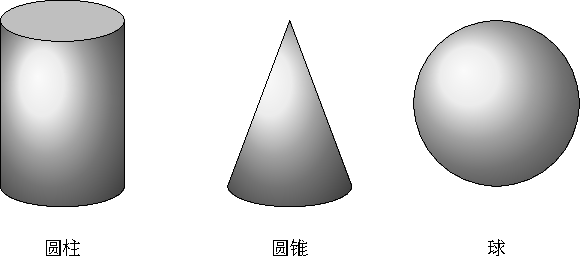
\includegraphics{1-1.pdf}
	\caption{}\label{fig:1-1}
\end{figure}

自古以来,人们经过实践、观察、分析,已总结出一系列的有关空间方面的知识,例如,从中国、埃及、巴比伦、玛雅等古文明中,可以看出对空间的知识都已掌握得相当丰富了。对于空间知识有系统的研究,从西方的古文明中可知,起始于古埃及和巴比伦,而在古希腊得到蓬勃的发展,获得较辉煌的成就。大体说来,古希腊在空间知识方面的成就,由欧几里得集其大成于他所著的《几何原本》\footnote{欧几里得(Euclid,约公元前 300 年左右)所著此书原名 \textit{Elements}, 我国明代数学家徐光启(公元 1562--1633)把书中部分几何内容	译成中文定名为“几何原本”。“几何学”这个中文的名称即来源于此。}这部书中。在这部书里,欧几里得把当时所知道的几何知识经过整理,建立起一个初步完整的理论体系,使这部书反映出几何学是一门偏重于推理、论证的高度理论性的科学。但是,和任何其它科学一样,几何学的理论基础也是建立在实验所得的一些基本事实之上的。在这一章里,我们就通过实验、观察、归纳来研究所得到的知识,为以后进一步学习论证几何作准备。

\section{点、直线和平面}
点、直线和平面是空间最简单的,也是最基本的图形。同学们在日常生活中,对它们早已有直观的认识了。在这一节里,我们再对它们的本质和相互关系作进一步的分析,确立点、直线和平面这三个基本的几何概念,并总结点、直线和平面之间相互关系方面的一些基本性质。

\subsection{点和直线}
在空间,最原始的,也是最基本的概念就是“位置”。通常,我们就用“点”来标记“位置”。例如在一张地图上,我们就以小圆点来标记各地的位置(见\cref{fig:1-2})。
\begin{figure}
	\begin{minipage}[b]{0.48\linewidth}
		\centering
		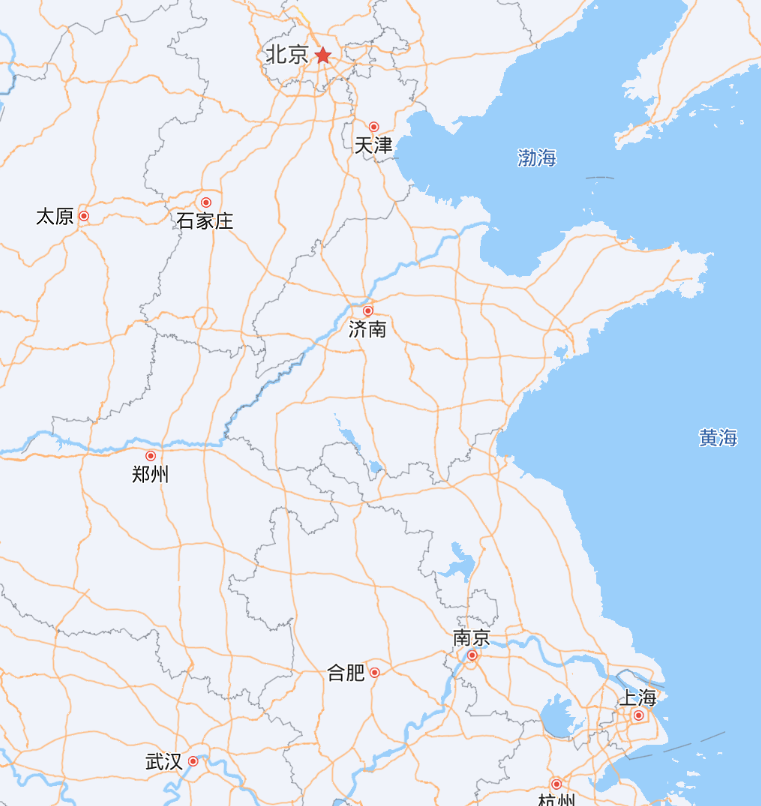
\includegraphics[width=0.9\linewidth]{1-2.png}
		\caption{}\label{fig:1-2}
	\end{minipage}
	\begin{minipage}[b]{0.48\linewidth}
		\centering
		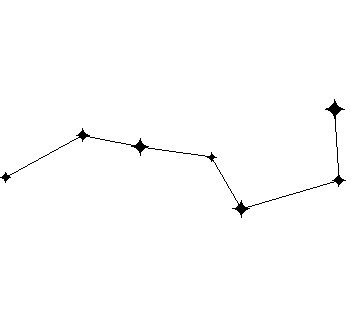
\includegraphics{1-3.pdf}
		\caption{}\label{fig:1-3}
	\end{minipage}
\end{figure}
你可能发现,在地图上北京用“$\star$”,南京用“{$\scriptstyle\odot$}”印制的,这只是为了把首都和地方城市区别开来。其实,北京、南京的“位置”与地图上印制的图形“$\star$”或“{$\scriptstyle\odot$}”的形状和大小是没有关系的。这样,仅仅考虑“位置”的图形就是点。在天象图上也是以小圆点来标记各星体的位置的(见\cref{fig:1-3})。

在几何学的讨论中,我们用不同的大写字母 $A,B,C,\ldots$ 表示不同的点,如\cref{fig:1-4} 中的五个点,就在点旁分别标记以 $A$、$B$、$C$、$D$、$E$,并分别读作点 $A$、点 $B$、点 $C$、点 $D$、点 $E$。

\begin{figure}
  \begin{minipage}[b]{0.48\linewidth}
    \centering
		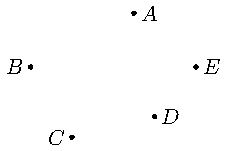
\includegraphics{1-4.pdf}
    \caption{}\label{fig:1-4}
  \end{minipage}
  \begin{minipage}[b]{0.48\linewidth}
    \centering
    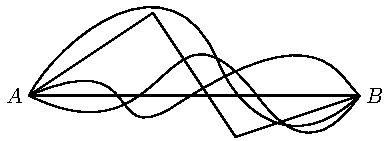
\includegraphics{1-5.pdf}
    \caption{}\label{fig:1-5}
  \end{minipage}
\end{figure}


在日常生活中,我们经常需要从一个地方走到另一个地方。例如,同学们早起上学,就得由自己的家所在的位置走到学校所在的位置。因此,在空间第二个原始的基本概念就要算是“通路”了。所谓“通路”,就是从一个位置移到另一个位置的路线。通常在地图上,我们用线来标记各地之间的种种通路,如铁路、公路等。在几何学的讨论中,“线”就是表示通路的。它的直观含义就是:一个“动点”由一个位置移动到另一个位置所走过的“路线”。如\cref{fig:1-5} 所示,设 $A$、$B$ 两点分别表示空间的两个位置,那么连结 $A$、$B$ 两点的可能通路是很多很多的。

在通常情况下,大家都希望所要走的通路愈短愈好,所以很自然的问题就是:

“在所有连结 $A$、$B$ 两点的各种通路中,哪一条通路最短?”

光线的存在,直截了当地显示给我们下述空间的基本性质:

“连结 $A$、$B$ 两点的最短通路唯一存在,它就是连结 $A$、$B$ 两点的\Concept{直线段}”(在均匀介质中,光走直线\footnote{由光学实验,我们知道光线其实走着最省时间的通路,而并不是走着最短的通路,再者,光的速度是随着“介质”而定的,例如在真空中走的最快,在空气中速度则稍慢(愈稀薄则其速度愈近于真空者),在水中则速度更慢,因为通常我们总是在均匀介质中观察光线,所以光线的速度是个不变的常数。这样,最省时间的通路也就是最短的通路。这就是我们常见常用的事实:光线在均匀介质中走直线。})。

\begin{figure}
	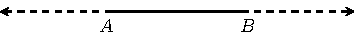
\includegraphics{1-6.pdf}
	\caption{}\label{fig:1-6}
\end{figure}


如\cref{fig:1-6} 所示,由 $A$ 点射向 $B$ 点的光线可以由 $A$ 向 $B$ 的方
向无限延伸;而由 $B$ 点射向 $A$ 点的光线也可以由 $B$ 向 $A$ 的方向无限延伸,所以对于空间任意两点 $A$、$B$,不但存在着唯一的最短通路“直线段 $AB$”,而且也唯一地确定了一条把直线段 $AB$ 两端无限延长的直线,这条直线就叫做由 $A$、$B$ 两点所确定的\Concept{直线},通常称为“直线 $AB$”,而直线段 $AB$ 是直线 $AB$ 介于 $A$、$B$ 两点之间的那一段。

归纳上面的讨论,我们可以作出如下的总结:

\begin{enumerate}[series=conclusion]
	\item “位置”和“通路”是两个最原始的空间概念。在几何学中,以点表示位置,以线表示通路。
	\item 对于任何两点 $A$、$B$,在所有连结、$AB$ 的可能通路中,存在唯一的最短通路,就是连结 $A$、$B$ 两点的直线段。
\end{enumerate}

直线段 $AB$ 也简称线段 $AB$,以后我们用符号 $\overline{AB}$ 表示线段
$AB$。点 $A$,点 $B$ 叫做线段 $AB$ 的\Concept{端点}。有时,一条线段也可以
用一个小写字母来表示,例如线段 $a$、线段 $b$ 等(\cref{fig:1-7a})。

\begin{figure}
	\begin{minipage}[b]{0.4\linewidth}\centering
		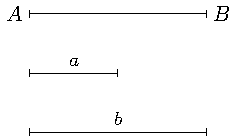
\includegraphics{1-7a.pdf}
		\subcaption{}\label{fig:1-7a}
	\end{minipage}
	\begin{minipage}[b]{0.4\linewidth}\centering
		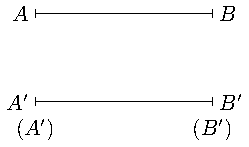
\includegraphics{1-7b.pdf}
		\subcaption{}\label{fig:1-7b}
	\end{minipage}
	\par\smallskip
	\begin{minipage}[b]{0.4\linewidth}\centering
		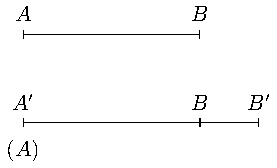
\includegraphics{1-7c.pdf}
		\subcaption{}\label{fig:1-7c}
	\end{minipage}
	\begin{minipage}[b]{0.4\linewidth}\centering
		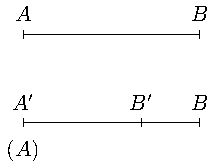
\includegraphics{1-7d.pdf}
		\subcaption{}\label{fig:1-7d}
	\end{minipage}
	\caption{}\label{fig:1-7}
\end{figure}

把 $\overline{AB}$ 放在 $\overline{A'B'}$ 上面,使点 $A$ 和点 $A'$ 重合,$\overline{AB}$ 沿着 $\overline{A'B'}$ 方向落下,那么有以下三种可能情况:
\begin{enumerate}[1)]
	\item 点 $B$ 和点 $B'$ 重合,这时 $\overline{AB}=\overline{A'B'}$ (\cref{fig:1-7b});
	\item 点 $B$ 落在 $A'$ 和 $B'$ 之间,这时 $\overline{AB}<\overline{A'B'}$ (\cref{fig:1-7c});
	\item 点 $B$ 落在 $\overline{A'B'}$ 的延长线上,这时 $\overline{AB}>\overline{A'B'}$(\cref{fig:1-7d})。
\end{enumerate} 

有一根拉直的绳子 $\overline{AB}$,如果把它分成长度相等的两段。但是不许用尺来量,应怎么办?

同学们一定会想到,把绳子 $\overline{AB}$ 的两端点 $A$、$B$ 重叠在一起,并且把绳子拉直,那么在绳子的中间就折出一个 $C$ 点来(\cref{fig:1-8a}), 而被折成的两段绳子 $\overline{AC}$ 和 $\overline{CB}$ 恰好长度相等,这就是说 $C$ 点把 $\overline{AB}$ 平分了。所以我们把平分线段的点叫做\Concept{线段的中点}。如果点 $C$ 是 $\overline{AB}$ 的中点,则 $\overline{AB}=2\overline{AC}=2\overline{CB}$。

\begin{figure}
  \begin{minipage}[b]{0.48\linewidth}
    \centering
		\begin{minipage}{0.5\linewidth}\raggedleft
		  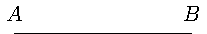
\includegraphics{1-8a.pdf}
		\end{minipage}%
		\begin{minipage}{0.1\linewidth}
		  \subcaption{}\label{fig:1-8a}
		\end{minipage}
		\par\bigskip
		\begin{minipage}{0.5\linewidth}\raggedleft
		  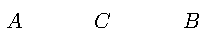
\includegraphics{1-8b.pdf}
		\end{minipage}%
		\begin{minipage}{0.1\linewidth}
		  \subcaption{}\label{fig:1-8b}
		\end{minipage}
    \caption{}\label{fig:1-8}
	\end{minipage}
	\begin{minipage}[b]{0.48\linewidth}
    \centering
		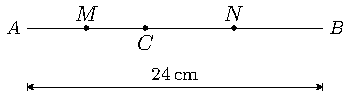
\includegraphics{1-9.pdf}
    \caption{}\label{fig:1-9}
  \end{minipage}
\end{figure}

\begin{example}\label{exp:half_length}
	已知 $\overline{AB}=\qty{24}{cm}$,点 $C$ 在 $\overline{AB}$ 上,点 $M$、$N$ 分别是 $\overline{AC}$ 和 $\overline{CB}$ 的中点,求 $\overline{MN}$ 的长度(见\cref{fig:1-9})。
\end{example}

\begin{solution}
\[\begin{split}
	\overline{MN}&=\overline{MC}+\overline{CN}=\frac{1}{2}\overline{AC}+\frac{1}{2}\overline{CB}\\
	&=\frac{1}{2}\left(\overline{AC}+\overline{CB}\right)=\frac{1}{2}\overline{AB}=\qty{12}{cm}
\end{split}\]
\end{solution}

\begin{enumerate}[resume=conclusion]%\setcounter{enumi}{2} 
	\item 线段可以向两端无限延长,这样就得到一条直线。一条直线可以用表示它上面任	意两点的大写字母来表示,如直线 $CD$。有时为了简便,也可以在这条直线旁标以一个小写字母,如 $\ell$,表示成直线 $\ell$(\cref{fig:1-10})。
	\begin{figure}
		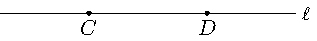
\includegraphics{1-10.pdf}
		\caption{}\label{fig:1-10}
	\end{figure}
	\item 对于任何两点 $A$、$B$,都存在着唯一一条通过 $A$、$B$ 的直线。这个性质就简述为:\emph{两点确定一条直线}。
\end{enumerate}

根据上述性质,我们可以说明其它有关的性质和问题。

\begin{example}
	如果两条直线 $\ell$ 和 $m$ 有一个公共点(交点)$A$(\cref{fig:1-11}),它们还能有其它的公共点吗?为什么?
\end{example}

\begin{figure}
	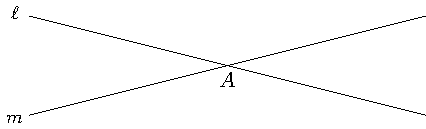
\includegraphics{1-11.pdf}
	\caption{}\label{fig:1-11}
\end{figure}

\begin{solution}
除 $A$ 点外,直线 $\ell$ 和 $m$ 不能再有其它的公共点了。

因为,如果还有另一个公共点 $B$,那么,$\ell$ 和 $m$ 就都是通过 $A$、$B$ 两点的直线。但是通过 $A$、$B$ 两点只有唯一的一条直线,于是,$\ell$ 和 $m$ 就是通过 $A$、$B$ 两点的那条唯一的直线,它们就不是两条不同的直线了。所以,它们除了 $A$ 点外,不可能再有其它的公共点了。

这件事实可以简述为:\emph{两条相交直线确定一交点}。
\end{solution}


\begin{example}
	\cref{fig:1-12} 表示人和物之间放一隔板,使人不能直接看到物的示意图,$A$ 表示物,$E$ 表示人眼,$\overline{BC}$ 表示隔板。为了能看见物的形象,放置一面镜子,图中 $g$ 表示镜面,这时按图1.12(1)中隔板 $\overline{BC}$ 的位置来说,人眼 $E$ 便能看见物 A 的形象,这是为什么?但按图1.12(2)隔板 $\overline{BC}$ 的位置来说,人眼 $E$ 便不能看到物 $A$ 的形象,这又是为什么?
\end{example}

\begin{figure}
	\begin{minipage}[b]{0.45\linewidth}\centering
	  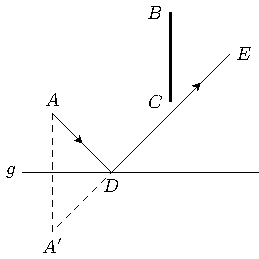
\includegraphics{1-12a.pdf}
		\subcaption{}\label{fig:1-12a}
	\end{minipage}
	\begin{minipage}[b]{0.45\linewidth}\centering
	  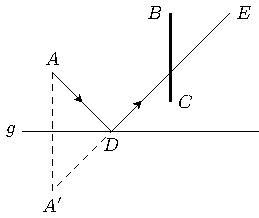
\includegraphics{1-12b.pdf}
		\subcaption{}\label{fig:1-12b}
	\end{minipage}
	\caption{}\label{fig:1-12}
\end{figure}

\begin{solution}
按照镜面映象的道理,人眼 $E$ 是从入射线 $AD$ 和反射线 $DE$ 看见 $A$ 的形象的,而点 $D$ 是点 $E$ 和点 $A$ 的象 $A'$ 的连线 $EA'$ 和 $g$ 的交点,所以 $A$ 的象 $A'$ 是沿着直线 $A'E$ 映入人眼 $E$ 的。因为通过 $A'$ 和 $E$ 只有唯一的一条直线,于是 $A'E$ 和隔板 $\overline{BC}$ 不交(\cref{fig:1-12a})时,在 $E$ 处就看得见 $A$ 的象 $A'$;$A'E$ 和 $\overline{BC}$ 相交,也就是被隔板 $\overline{BC}$ 挡住(\cref{fig:1-12b})时,在 $E$ 处便看不见 $A$ 的象 $A'$ 了。
\end{solution}

\begin{example}\label{exp:segment_count}
如果在已知$\overline{AB}$上依次取 99 个点($C_1,C_2,C_3,\ldots,C_{99}$),那么$\overline{AB}$ 上一共有多少条以这些点为端点的线段?($\overline{AB}$ 也计算在内)
\end{example}	

\begin{solution}
我们分以下几步来研究这个问题:
\begin{enumerate}[leftmargin=2.0em,label=第\chinese*步,font=\bfseries]
	\item 先进行观察、实验。因为每两个点就确定一条线段。因此,
	\begin{enumerate}[leftmargin=0.0em,label=\arabic*)]
    \item 在 $\overline{AB}$ 上取一个点 $C_1$ 时,我们看到\cref{fig:1-13a} 中共有 3 条线段 $\overline{AB}$、$\overline{AC_1}$ 和 $\overline{C_1B}$。
    \begin{figure}
			\begin{minipage}[b]{0.7\linewidth}\centering
				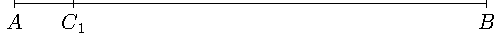
\includegraphics{1-13a.pdf}
			\end{minipage}%
			\begin{minipage}[b]{0.1\linewidth}
				\subcaption{}\label{fig:1-13a}
			\end{minipage}
			\begin{minipage}[b]{0.7\linewidth}\centering
				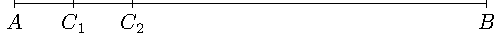
\includegraphics{1-13b.pdf}
			\end{minipage}%
			\begin{minipage}[b]{0.1\linewidth}
				\subcaption{}\label{fig:1-13b}
			\end{minipage}
			\begin{minipage}[b]{0.7\linewidth}\centering
				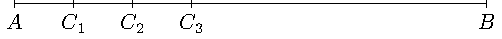
\includegraphics{1-13c.pdf}
			\end{minipage}%
			\begin{minipage}[b]{0.1\linewidth}
				\subcaption{}\label{fig:1-13c}
			\end{minipage}
			\begin{minipage}[b]{0.7\linewidth}\centering
				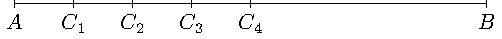
\includegraphics{1-13d.pdf}
			\end{minipage}%
			\begin{minipage}[b]{0.1\linewidth}
				\subcaption{}\label{fig:1-13d}
			\end{minipage}
			\begin{minipage}[b]{0.7\linewidth}\centering
				$\vdots$
			\end{minipage}%
			\begin{minipage}[b]{0.1\linewidth}\centering
				$\vdots$
			\end{minipage}
			\par\smallskip
			\begin{minipage}[b]{0.7\linewidth}\centering
				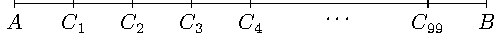
\includegraphics{1-13e.pdf}
			\end{minipage}%
			\begin{minipage}[b]{0.1\linewidth}
				\setcounter{subfigure}{13}
				\subcaption{}\label{fig:1-13e}
			\end{minipage}
			\caption{}\label{fig:1-13}
		\end{figure}
		\item 在 $\overline{AB}$ 上取两个点 $C_1$、$C_2$ 时,我们看到\cref{fig:1-13b} 中共有 6 条线段 $\overline{AB}$、$\overline{AC_1}$、$\overline{C_1B}$、$\overline{AC_2}$、$\overline{C_2B}$ 和 $\overline{C_1C_2}$。
	\item 在 $\overline{AB}$ 上取三个点 $C_1$、$C_2$、$C_3$ 时,我们看到\cref{fig:1-13c} 中有 10 条线段(请同学们自己找出来)。 
	\end{enumerate}
	\item\label{itm:law} 列表分析找规律
	\begin{center}
		\begin{tblr}{colspec={X[c]X[c]},hline{2}=0.8pt}
		$\overline{AB}$ 上取的点数 & $\overline{AB}$ 上线段的总数\\
		1&3\\
		2&6\\
		3&10\\
		$\vdots$&$\vdots$\\
		99& ?\\
		\end{tblr}
	\end{center}

  从表上发现:
	\begin{itemize}
		\item 在 $\overline{AB}$ 上取 1 个点时,$\overline{AB}$ 上的线段总数 $3=1+2$,
		\item 在 $\overline{AB}$ 上取 2 个点时,$\overline{AB}$ 上的线段总数 $6=1+2+3$,
		\item 在 $\overline{AB}$ 上取 3 个点时,$\overline{AB}$ 上的线段总数 $10=1+2+3+4$。
	\end{itemize}

	这时,如果在 $\overline{AB}$上取 4 个点,那么$\overline{AB}$上共有多少条线段呢?由上面发现的规律,可以猜想是 $1+2+3+4+5=15$,数一下\cref{fig:1-13d} 中的线段数,恰好是 15 条。这样自然要问:当在 $\overline{AB}$ 上取 99 个点时,将会有怎样的结果呢?

	\item 归纳、计算

	如果在 $\overline{AB}$上取 99 个点,设这时 $\overline{AB}$ 上的线段总数为 $S$,由在\ref{itm:law}中发现的规律,不难得出:
	\[S=1+2+3+4\cdots +(99+1)=1+2+3+4\cdots +100\]

	这是一个很有趣的计算题,如果按顺序加起来,计算是很麻烦的,我们动动脑筋能否有简便的计算方法呢?

	由于 $S=1+2+3+\cdots +98+99+100$,也就是:
	\[S=100+99+98+\cdots +3+2+1\]

	$\therefore\quad 2S=\underbrace{101+101+101\cdots+101+101+101}_{100\text{项}}=100\times 101$

	$\therefore\quad S=\dfrac{100\times 101}{2}=5050$
\end{enumerate}
\end{solution}

\begin{Practice}
\begin{question}
	\item\label{prac:1-1-1} 图中有几条线段,把它们都写出来。
	\begin{figurehere}
		\begin{minipage}{\linewidth}\centering
			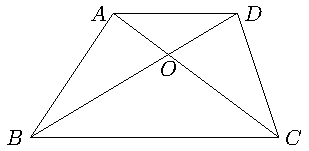
\includegraphics{pr1-1-1.pdf}
			\caption*{第 \ref{prac:1-1-1} 题}
		\end{minipage}
	\end{figurehere}
	\item $A$、$B$、$C$ 三点不在一条直线上,通过其中任何两点画一条直线,一共能画出几条直线?
	\item $A$、$B$、$C$、$D$ 四点中,任何三点都不在一条直线上,通过其中任何两点画一条直线,一共能画出几条直线?
	\item 如果 $A$、$B$、$C$、$D$、$E$ 五点中任何三点都不在一条直线上,通过其中任何两点画一条直线,那么一共能画多少条直线?
	\item 如果有 100 个点,其中任何三点都不在一条直线上,通	过其中任何两点画一条直线,那么一共能画多少条直线?
	\item 工人师付在用方砖铺地时,常常打两个木桩,拉线来铺砖,这样砖就铺得整齐,这是根据了什么道理?
	\item 如果有两个小孩甲、乙在对话,甲问乙:“你的家住在哪里?”乙回答说:“我的家住在直线 $AB$ 的尽头。”试问你能沿着直线 $AB$ 找到乙的家吗?为什么?
	\item 参看\cref{exp:segment_count} 的归纳、计算,如果在 $\overline{AB}$ 上取 $n$ 个点。那么 $\overline{AB}$ 上一共有多少条线段?($\overline{AB}$ 也计算在内)
	\item 已知:$\overline{MN}=\qty{100}{m}$,$P$ 点在 $\overline{MN}$上,$\overline{MP}=\qty{45}{m}$,$S$ 点是 $\overline{PN}$ 的中点,求 $\overline{PS}$的长度是多少米?
	\item 在\cref{exp:half_length} 中,$\overline{MN}$ 的长度与 $C$ 点在 $\overline{AB}$ 上的位置有无关系?
\end{question}
\end{Practice}


\subsection{长度的度量}
在给定两点 $A$、$B$ 之间的所有通路之中,以 $AB$ 为最短,它的“长度”就叫做 $A$、$B$ \Concept{两点间的距离}。所以,两点间的距离是连结这两点的线段的长。

长度是我们经常用的一种几何量,现在让我们分别从实用和数学的观点稍微细致地分析一下“长度”这种几何量的直观含义,并且谈一谈长度的度量。

一般来说,常用的量基本上可以归成两类:其中一类,例如一群羊、一堆蛋,它们具有天然的个别单元,即一只羊、一个蛋。处理这种量,我们只要去数一数它们的“个数”就可以了。因为它们是可数的。用来数“个数”的数学体系就是我们在代数学中一开始就详加讨论的自然数系:$\{1,2,3,\ldots\}$。另一类,例如我们现在要讨论的长度等,这种量虽然不具有天然个别单元,但是,具有一个基本特点:可以无限细分。例如,任给一个线段,不管它怎样短,还是可以把它分割成更短的线段。因此,这种量不可能有天然不可分割的单元,我们处理这种量的办法就是度量。

因为长度这种量并不具有天然不可分割的单位,所以,我们只好选用人为的长度单位。例如“米”就是世界上通用的长度单位。取定长度单位以后,要度量一条线段的长度,也就是要求得它和长度单位之间的“比值”。例如取定长度单位为 \unit{m},所求得的比值是 $1237:1000$,就说这条线段的长度是 \qty{1.237}{m}。但是在实践中,这个比值是怎样求出来的呢?先举几个简单的实例看一看。

\begin{example}\label{exp:divide_mult}
设长度单位是 $u$,所要度量的线段是 $a$ (\cref{fig:1-14})。线段 $a$ 恰好可以分割成 5 段和 $u$ 等长的线段,那么所求的比值是 5,$a$ 的长度就是 $5u$。

一般地说,如果所要度量的线段 $a$ 恰好可以分割成 $m$ 段和 $u$ 等长的线段,那么所求的比值就是整数 $m$,$a$ 的长度就是 $mu$。
\end{example}

\begin{figure}
  \begin{minipage}[b]{0.48\linewidth}
    \centering
		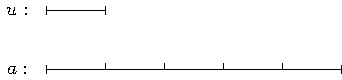
\includegraphics{1-14.pdf}
    \caption{}\label{fig:1-14}
	\end{minipage}
	\begin{minipage}[b]{0.48\linewidth}
    \centering
    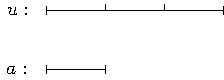
\includegraphics{1-15.pdf}
    \caption{}\label{fig:1-15}
	\end{minipage}
\end{figure}

\begin{example}\label{exp:divide_fraction}
设长度单位是 $u$,所要度量的线段是 $b$(\cref{fig:1-15})单位长 $u$ 恰好可以分割成 3 段和 $b$ 等长的线段,那么所求的比值是 $\dfrac{1}{3}$,$b$ 的长度就是$\dfrac{1}{3}u$。

\bigskip
一般地说,如果长度单位 $u$ 恰好可以分割成 $n$ 段和 $b$ 等长的线段,那么所求的比值是 $\dfrac{1}{n}$,$b$ 的长度就是 $\dfrac{1}{n}u$。
\end{example}

\begin{example}\label{exp:rational_divide}
设长度单位是 $u$,所要度量的线段是 $c$(\cref{fig:1-16})。$c$ 比 $4u$ 长些,但又比 $5u$ 短些,如果我们把 $u$ 三等分,线段$c$截取 4 段 $u$ 后所余的一段恰好是 $\dfrac{1}{3}u$ 的 2 倍,那么$c$ 的长度就是 $4\dfrac{2}{3}u$。

\begin{figure}
	\centering
  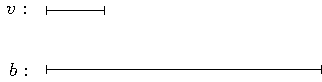
\includegraphics{1-16.pdf}
	\caption{}\label{fig:1-16}
\end{figure}
{\linespread{1.65}\selectfont
一般地说,如果把长度单位 $u$ 适当地等分成 $n$ 段,即每一段 $u'$ 的长度是$\dfrac{1}{n}\cdot u$,所要量的线段 $c$ 恰好可以分割成 $m$ 段和线段 $u'$ 等长的线段,那么 $c$ 的长度就是 $\dfrac{m}{n}u$。

在\cref{exp:rational_divide} 中,用长度单位 $u$ 去度量 $c$ 时,怎样才能知道在 $c$ 上截取 4 段 $u$ 后,所余的一段恰好是 $u$ 的 $\dfrac{1}{3}$ 的整数倍?实际上可以这样来确定:在 $c$ 上截取 4 段 $u$ 后,以所余的一段 $\overline{C_4D}$ 去量 $u$,在 $u$ 上截去一段 $\overline{C_4D}$ 后,所余的一段 $\overline{U_1V}$ 又较 $\overline{C_4D}$ 短,这时再以 $\overline{U_1V}$ 去度量 $\overline{C_4D}$,恰好$\overline{C_4D}$ 是 $\overline{U_1V}$ 的 2 倍。这样便看出 $\overline{U_1V}$ 是 $u$ 的 $\dfrac{1}{3}$,把 $u$ 三等分后,$\overline{C_4D}$ 就恰好是 $\dfrac{1}{3}u$ 的 2 倍了。\par}
\end{example}

\begin{example}\label{exp:rational_divide2}
	设长度单位是 $u$,求线段 $d$ 的长度(\cref{fig:1-17})。
\begin{figure}
	\centering
  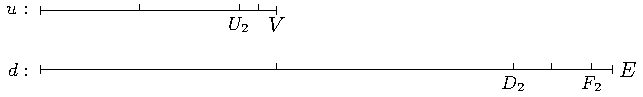
\includegraphics{1-17.pdf}
	\caption{}\label{fig:1-17}
\end{figure}
\end{example}

\begin{solution}
在 $d$ 上用圆规截取 2 段 $u$ 后,所余的一段 $\overline{D_2E}$ 较 $u$ 短;在 $u$ 上截取 2 段 $\overline{D_2E}$ 后,所余的 $\overline{U_2V}$ 较 $\overline{D_2E}$ 短;在 $\overline{D_2E}$ 上截取 2 段 $\overline{U_2V}$ 后,所余的一段 $\overline{F_2E}$ 较 $\overline{U_2V}$ 短;但 $\overline{U_2V}$ 恰好是 $\overline{F_2E}$ 的 2 倍。于是
\[\begin{split}
	\overline{D_2E}&=\overline{D_2F_2}+\overline{F_2E}=2\overline{U_2V}+\overline{F_2E}\\
&=2\cdot 2\overline{F_2E}+\overline{F_2E}=5\overline{F_2E}
\end{split}\]
\[u=2\overline{D_2E}+\overline{U_2V}=2-5\overline{F_2E}+2\overline{F_2E}=12\overline{F_2E}\]
$\therefore\quad \overline{F_2E}=\dfrac{1}{12}u,\quad \overline{D_2E}=\dfrac{5}{12}u,\quad d=2\dfrac{5}{12}u$
\end{solution}

\bigskip
由\cref{exp:rational_divide,exp:rational_divide2} 可以看出,当被度量线段($c$ 和 $d$)不能恰好被分割而成为长度单位的整数倍,也就是它们不能被长度单位量尽时,都是求出另一条线段(\cref{exp:rational_divide} 中是 $\overline{U_1V}$,\cref{exp:rational_divide2} 中是 $\overline{F_2E}$),使得它能量尽长度单位和被量线段。再按\cref{exp:divide_fraction} 的方法求出以长度单位为单位的这条线段的长度,然后便可求出原来被量线段的长度了。

能够量尽两条线段 $a$ 和 $b$ 的线段,我们叫它做线段 $a$ 和 $b$ 的\Concept{公度}。两条线段的公度中最长的,叫做\Concept{这两条线段的最大公度}。$\overline{U_1V}$ 和$\overline{F_2E}$ 就分别是线段 $u$ 和 $c$,$u$ 和 $d$ 的最大公度。在\cref{exp:divide_mult} 中线段$u$ 就是线段 $u$ 和 $a$ 的最大公度;\cref{exp:divide_fraction} 中的线段 $b$ 就是线段 $u$ 和 $b$ 的最大公度,象\cref{exp:rational_divide,exp:rational_divide2} 中求线段 $u$ 和 $c$、$u$ 和 $d$ 的最大公度的方法,叫做\Concept{辗转相截法}。

通过上面各例,我们很自然地会想到:任何两条线段 $a, b$,它们的长度比值是否总是一个分数(整数也可看作分数)?换句话说,对于任何两条线段 $a$、$b$,是否存在着它
们的公度?

这个问题从正、反两面来分析它的重要性。首先,如果任何两条线段的长度的比值总是一个分数,那么分数全体(即代数开始所讲的有理数)就足以处理长度的度量问题了。其次,反过来说,如果两条线段的长度的比值不一定是分数,那么有理数就不足以处理长度的度量问题。因而我们就得学会一种含有“非分数”的数系才能充分解决度量问题。这个问题是整个数学发展史上的一件大事,我们以后再详细讨论。

\begin{Practice}
\begin{question}
	\item 已知线段 $a$、$b$、$u$,其中线段 $a=9u$,$b=3u$,问线段 $a$、$b$ 的最大公度是线段 $u$ 的几倍?
	\item 已知线段 $a=\qty{48}{mm}$,$b=\qty{18}{mm}$。先用辗转相截法求出	$a$、$b$ 的最大公度,并量它等于多少毫米;再用求最大公	约数的辗转相除法求出 48、18 的最大公约数。比较前后所得的结果。
	\item 根据图形填写下面空白:
	\begin{figurehere}
		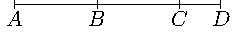
\includegraphics{pr1-2-3.pdf}
	\end{figurehere}
	\begin{tasks}(2)
		\task $\overline{AC}=\overline{BC}+(\qquad)$	
		\task	$\overline{CD}=\overline{AD}-(\qquad)$	
		\task $\overline{AC}+\overline{CD}=(\qquad)+\overline{BD}$
	\end{tasks}
\end{question}
\end{Practice}

\subsection{直线和平面}
在空间,另一种常见的形象就是各种各样的面。例如地球的表面,它的整体看起来是一个略为扁平的球面,而局部的形象又随着当地的地貌而不同。有的地方是一片原,有的地方是起伏的丘陵,有的地方是一片湖面,也有的地方是崇山峻岭和深谷。又如教室的一面墙壁,上课用的黑板,以及桌面等,看起来又都是“平直”的面。

通常检查一个桌面是否“平直”,最简单的方法就是用一根直尺放在桌面上(\cref{fig:1-18}),如果放在任何位置上,直尺的边都和桌面密合,那么桌面就是“平直”的。我们就说桌面是平面。但是象\cref{fig:1-19} 的面上,虽然直尺放在  $\ell_1,\ell_2,\ldots,\ell_n$ 等位置时,直尺边和这个面密合,而在 $AB$ 位置上直尺边和面就不密合了。这就是说并不是在任何位置上直尺的边总和这个面密合,这个面不是一个平面,实际上是一个曲面。
\begin{figure}
  \begin{minipage}[b]{0.48\linewidth}
    \centering
		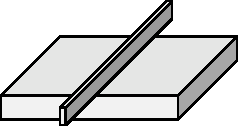
\includegraphics{1-18.pdf}
    \caption{}\label{fig:1-18}
  \end{minipage}
  \begin{minipage}[b]{0.48\linewidth}
    \centering
		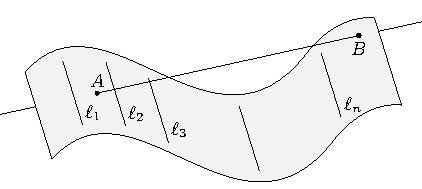
\includegraphics{1-19.pdf}
    \caption{}\label{fig:1-19}
  \end{minipage}
\end{figure}

在几何学的讨论中,平面就是一个到处平直而且向各个方向无限延展的面,它的特点就是在它上面任取两点 $A$ 和 $B$(\cref{fig:1-20}),直线 $AB$ 就完全在这个平面内。

\begin{figure}
  \begin{minipage}[b]{0.48\linewidth}
    \centering
		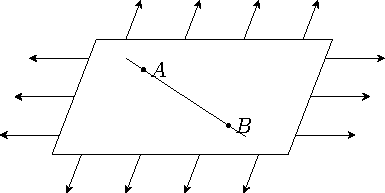
\includegraphics{1-20.pdf}
    \caption{}\label{fig:1-20}
  \end{minipage}
  \begin{minipage}[b]{0.48\linewidth}
    \centering
    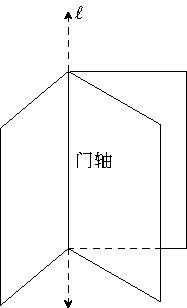
\includegraphics{1-21.pdf}
    \caption{}\label{fig:1-21}
  \end{minipage}
\end{figure}

我们观察一扇门,把它看作平面的一部分,那么它的轴线既在墙壁的平面内(\cref{fig:1-21}),又在这扇门所在的平面内,不可能连结两个“合页”的直线不都在这两个平面内。推动这扇门,它每到一个新的位置都表现了通过轴线的一个平面。这些事实说明了:\emph{空间相交的两个平面的“交界”是一条直线。通过一条直线可有无数个平面。}

\begin{Practice}
\begin{question}
	\item 举出一条直线和一个平面没有公共点的实例,以及一条直线和一个平面只有一个公共点的实例。
	\item 一点在一平面内,而其它的点都不在这个平面内,这种实例有什么?
	\item 举出两个平面没有公共点的实例。
	\item 两个平面只有一个公共点的实例存在吗?
	\item 如果空间被平面 $\alpha$ 分成的两部分之一中,有一只小虫子 $A$,这只小虫子 $A$ 要爬到	被平面所分空间的另一部分去,假如它不穿过平面 $\alpha$,能过去吗?为什么?
\end{question}
\end{Practice}

同学们作这样一个实验,张开手指,使拇指、食指和中指的尖这三点不在一条直线上,拿一张硬纸(它代表一个平面)往三个指尖上放,看看它是否能同时通过三个指尖?再拿一张硬纸仍然这样放,看这两张硬纸是否重合?这种特点对于一个指尖,两个指尖也适合吗?再使母指、食指、中指,无名指的指尖这四点不在一条直线上,看看能否保证总有一张硬纸同时通过这四点?仿照“两点确定一条直线”的特点,同学们能否总结出几个点确定一个平面的结论?

通过上面的实验,我们得出平面的另一个基本性质:\emph{空间不共线三点确定一个平面。}

同学们还可进一步思考以下的问题:
\begin{enumerate}
	\item 一直线及直线外一点能确定一个平面吗?
	\item 相交的两条直线能确定一个平面吗?
\end{enumerate}

\begin{Exercise}
% \addcontentsline{toc}{subsection}{习题1.1}
\begin{question}
	\item 什么是线段?什么是直线?两者有什么区别?
	\item 什么是线段的中点?如果有一根笔直的铁棍,假如用 $\overline{AB}$ 来表示它,不用尺量,也不许把它折弯,你有没有办法找出 $\overline{AB}$ 所表示的这根铁棍的中点来?
% 	\item 请同学们复习一下小学学过的公制、市制两种长度单位,
% 	并填下表:
% 	\begin{center}
% \begin{tabular}{ll}
% 	1公里(km)$=\underline{\qquad}$米(m) &\qquad 1里$=\underline{\qquad}$丈\\
% 1米(m)$=\underline{\qquad}$分米(dm)&\qquad 1丈$=\underline{\qquad}$尺\\
% 1分米(dm)$=\underline{\qquad}$厘米(cm)&\qquad 1尺$=\underline{\qquad}$寸\\
% 1厘米(cm)$=\underline{\qquad}$毫米(mm)&\qquad 1寸$=\underline{\qquad}$分
% \end{tabular}		
% 	\end{center}

% 	\item 	求出下列结果,并化成括号中指定的长度单位:
% \begin{tasks}
% \task 5尺4寸5分 $+$ 3尺4寸 $+$ 6尺7寸8分$=\underline{\qquad}$(米);
% \task 46厘米 $+$ 1米60厘米 $+$ 7米50厘米$=\underline{\qquad}$(尺);
% \task 4丈5尺6寸$\times3=\underline{\qquad}$(米);
% \task 5米40厘米$\div 1000=\underline{\qquad}$(毫米);
% \task 20mm$\times0.1\%=\underline{\qquad}$(m)
% \end{tasks}

\item\label{exec:1-1-3} 在一条直线上,顺次取 $A$、$B$、$C$ 三点,使 $\overline{AB}=\qty{4}{cm}$,$\overline{BC}=\qty{2}{cm}$,并且取 $\overline{AC}$ 的中点 $O$,求:
	\begin{tasks}(3)
		\task $\overline{AO}$ 的长
		\task $\overline{OB}$ 的长
		\task $\overline{OC}$ 的长
	\end{tasks}

\begin{figurehere}
	\begin{minipage}{\linewidth}\centering
		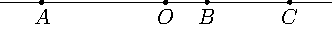
\includegraphics{ex1-1-3.pdf}
		\caption*{第 \ref{exec:1-1-3} 题}
	\end{minipage}
\end{figurehere}

\item 把一条 \qty{32}{cm} 的线段分成三段,中间的一段长为 \qty{8}{cm},问第一段中点到第二段中点的距离等于多少 \unit{cm}?
\item\label{exec:1-1-5} 图中表明四个点可以确定一条、四条或者六条直线。试划图说明五个点可以确定 1、5、6、8 或 10 条直线(其它情况不存在)。
\begin{figurehere}
	\begin{minipage}{\linewidth}\centering
		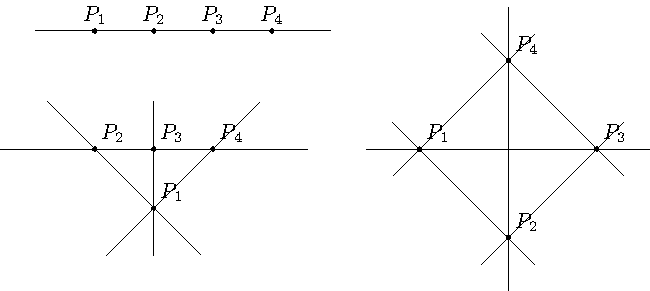
\includegraphics{ex1-1-5.pdf}
		\caption*{第 \ref{exec:1-1-5} 题}
	\end{minipage}
\end{figurehere}

\item\label{exec:1-1-6} 在三角形 $ABC$ 的 $\overline{BC}$ 边上如果取 $n$ 个点$P_1,P_2,P_3,\ldots,P_n$,并把这 $n$ 个点分别和 $A$ 点连结起来,就出现很多三角形,试研究三角形的总数有多少?(原来的三角形 $ABC$ 也包括在内)。

(提示:$\overline{BC}$ 上每一条线段都可与 $A$ 点构成一个三角形,因此求三角形的总数实际上就是求$\overline{BC}$上线段的总数)。
\begin{figurehere}
	\begin{minipage}{\linewidth}\centering
		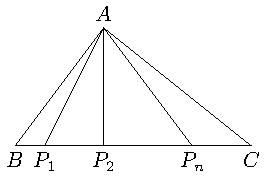
\includegraphics{ex1-1-6.pdf}
		\caption*{第 \ref{exec:1-1-6} 题}
	\end{minipage}
\end{figurehere}
\end{question}
\end{Exercise}

\section{方向、角度与平行}
\subsection{方向与角}
当我们在平坦的操场上要从一个位置(以 $A$ 点表示)走到另一个位置(以 $B$ 点表示),经验告诉我们最省事的走法是:“由 $A$ 点朝向 $B$ 点一直走”。(\cref{fig:1-22})

\begin{figure}
	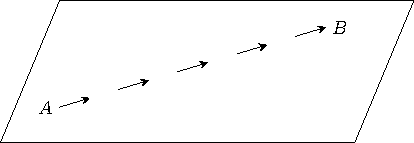
\includegraphics{1-22.pdf}
	\caption{}\label{fig:1-22}
\end{figure}

上面这种常用的走法,很明显地突出了“方向”这个常用的基本几何概念。再设想我们是正在茫茫大海中航行的船的舵手,或者是一架越洋飞行的飞机的驾驶员,那么“方向”这个概念就更是至关紧要的了!因为“航行的方向”是我们随时要确切掌握的要素!

现在让我们就上面的实例,对于所涉及的“方向”这个概念的直观含义,稍加分析。

假如我们从操场的 $A$ 点走向 $B$ 点去(\cref{fig:1-23}),最省事的“通路”当然就是 $\overline{AB}$(因为它是最短的通路)。所以我们先站在 $A$ 点,向 $B$ 点望一望,头脑中抽象地计画了所要走的路线应该是直线段(图中虚线所示)。然后便一步步地沿着设想的路线 $\overline{AB}$ 向 $B$ 点一直走。从几何的观点看,每跨一步就沿着某一个方向做了一个和自己步幅等长的“有向线段”。所以说,“由 $A$ 点朝向 $B$ 点一直走的走法”就是每一步都是沿着 $\overline{AB}$ 这个固定的方向走的那种走法。


\begin{figure}
	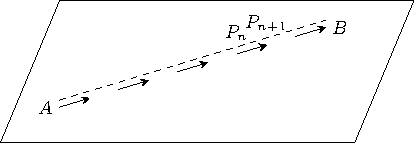
\includegraphics{1-23.pdf}
	\caption{}\label{fig:1-23}
\end{figure}

在由 $A$ 点可以直接看到 $B$ 点的情形下,要保持每一步的方向都是正对着 $B$ 点的方向是很简单的。因为我们随时可以用目光把行进中的位置(\cref{fig:1-23} 中的 $P_n$ 点)和 $B$ 点连一条直线,这条直线的方向也就是下一步(\cref{fig:1-23} 中的 $P_nP_{n+1}$)所要走的方向。但是在另外两个设想的航海和飞行的实例中,目的地是遥远而看不到的,而计划中要走的航线,所经过的绝大部分都是“漫无边际”的海洋和天空,毫无可供“瞄准”的标志。所以要随时保持航行的方向的正确性就变成确保安全到达目的地的最重要的依据了。

由 $A$ 点出发,沿着一个固定的方向(比如向着 $B$ 点的方向)前进时,它的路线就是一条\Concept{射线}。如\cref{fig:1-24} 所示,它就是居于 $A$ 点右侧的那条半直线。
\begin{figure}
  \begin{minipage}[b]{0.48\linewidth}
    \centering
		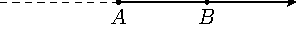
\includegraphics{1-24.pdf}
    \caption{}\label{fig:1-24}
  \end{minipage}
  \begin{minipage}[b]{0.48\linewidth}
    \centering
    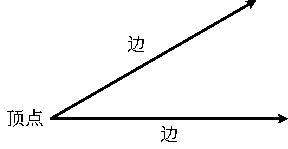
\includegraphics{1-25.pdf}
    \caption{}\label{fig:1-25}
  \end{minipage}
\end{figure}

所以我们把直线上一点一旁的部分叫做\Concept{射线},这一点叫做射线的\Concept{端点}。例如射线 $AB$(\cref{fig:1-24})。(注意:表示射线时,射线的端点字母必须写在前面)。在几何中,我们把以 $A$ 点为端点的一条射线看作是由 $A$ 点出发的一个方向。

我们把从同一端点引出的两条射线所组成的图形叫做\Concept{角},这个共同的端点叫做角的\Concept{顶点},这两条射线分别叫做角的\Concept{边}。我们把角看成是由构成这个角的两条射线所表示的方向差(\cref{fig:1-25})。

一个角通常用符号“$\angle$”(读作角)后边带三个大写字母来表示,中间一个字母表示角的顶点,两旁的两个字母分别表示角的两边上的任意点,如\cref{fig:1-26a} 中的角可记作 $\angle AOB$,读作“角 $AOB$”。如果用一个点作顶点的角只有一个,这个角也可以只用表示顶点的那个大写字母来表示,如\cref{fig:1-26a}  的 $\angle AOB$ 也可表示为 $\angle O$。有时,为了方便,还可以在角的里面靠近顶点写个数字、或小写希腊字母表示角,如\cref{fig:1-26b,fig:1-26c} 中的 $\angle 1$、$\angle 2$、$\angle 3$ 和 $\angle \alpha$、$\angle \beta$、$\angle \gamma$ 等。

\begin{figure}
	\begin{minipage}[b]{0.32\linewidth}\centering
		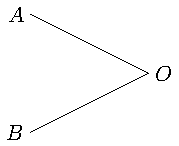
\includegraphics{1-26a.pdf}
		\subcaption{}\label{fig:1-26a}
	\end{minipage}%
	\begin{minipage}[b]{0.32\linewidth}\centering
		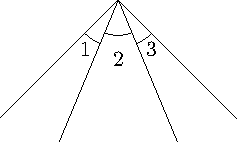
\includegraphics{1-26b.pdf}
		\subcaption{}\label{fig:1-26b}
	\end{minipage}%
	\begin{minipage}[b]{0.32\linewidth}\centering
		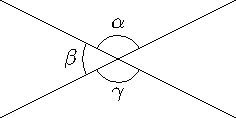
\includegraphics{1-26c.pdf}
		\subcaption{}\label{fig:1-26c}
	\end{minipage}
	\caption{}\label{fig:1-26}
\end{figure}

当一个角的两条边重合时,其夹角显然为 $O$(即方向没有差别)。另外一种特殊情形是当角的一边是另一边的反向延长线时,就称这个角为\Concept{平角}。如\cref{fig:1-27} 中射线 $CA$ 和射线 $CB$ 的方向相反,那么 $\angle ACB$ 就是一个平角。

\begin{figure}
  \begin{minipage}[b]{0.48\linewidth}
    \centering
		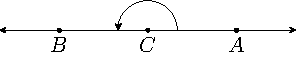
\includegraphics{1-27.pdf}
    \caption{}\label{fig:1-27}
	\end{minipage}
	\begin{minipage}[b]{0.48\linewidth}
    \centering
    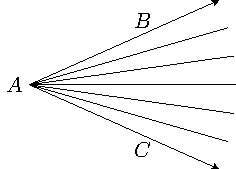
\includegraphics{1-28.pdf}
    \caption{}\label{fig:1-28}
	\end{minipage}
\end{figure}

根据上述,我们可以把日常常用的“方向”和角这两个概念,给以如下的说明:
\begin{enumerate}
	\item 自定点 $A$ 出发的所有方向和以 $A$ 点为端点的所有射线之间一一地相对应。换句话说,对应于自 $A$ 点出发的一个方向,就有唯一的一条射线(它就是自 $A$ 点出发沿着这个固定方向一直走的路线);反之任何一条以 $A$ 点为端点的射线也就唯一地表示了一个确定的方向。所以在几何学中,我们以一条射线表示一个方向。
	\item 一条以 $A$ 为端点的射线,由起始的任何一小段唯一确定(因为整个射线只是那一小段沿着那个方向的无限延伸),所以自 $A$ 点出发的一个方向实可以用它所对应的那条射线开头的任何一小段所表示。
	\item 设射线 $AB$ 和 $AC$ 分别表示由 $A$ 点出发的两个方向,那么 $\angle BAC$ 的直观含义就是射线 $AB$ 和 $AC$ 所表示的那两个方向的差。
	\item 除了零角和平角的特殊情形,如 $A$、$B$、$C$ 三点不共线,我们把射线 $AB$ 由原来的位置沿着平面绕 $A$ 点旋转到射线 $AC$ 的位置所“扫过的区域”叫做 $\angle BAC$ 的\Concept{内部},角的内部也可以叫做\Concept{角区}(\cref{fig:1-28})。
\end{enumerate}

\begin{Practice}
\begin{question}
	\item 什么是射线?射线的直观含义是什么?
	\item 什么是角?角的直观含义是什么?
	\item 线段、射线、直线有什么区别?
	\item\label{prac:1-4-4} 指出图中有几个角?并按图中字母把它们都写出来。
	\item\label{prac:1-4-5} 把图中数字表示的角,改用大写字母表示。
	\item\label{prac:1-4-6} 把图中用小写希腊字母表示的角,改用大写字母表示。
	\begin{figurehere}
		\begin{minipage}[b]{0.25\linewidth}\centering
			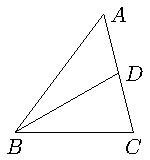
\includegraphics{pr1-4-4.pdf}
			\caption*{第 \ref{prac:1-4-4} 题}
		\end{minipage}%
		\begin{minipage}[b]{0.32\linewidth}\centering
			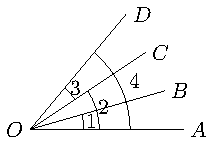
\includegraphics{pr1-4-5.pdf}
			\caption*{第 \ref{prac:1-4-5} 题}
		\end{minipage}%
		\begin{minipage}[b]{0.4\linewidth}\centering
			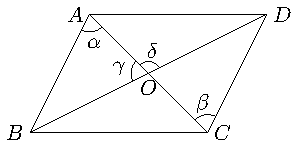
\includegraphics{pr1-4-6.pdf}
			\caption*{第 \ref{prac:1-4-6} 题}
		\end{minipage}
	\end{figurehere}
	\item\label{prac:1-4-7} 指出图中有多少个角,并按图中字母把它们都写出来。
	\item\label{prac:1-4-8} 已知 $P$、$Q$ 两点分别在 $\angle AOB$ 的两边上,试问是否存在不经过 $\angle AOB$ 的内部,由$	P$到$Q$的最短通路?
	\begin{figurehere}
		\begin{minipage}[b]{0.45\linewidth}\centering
		  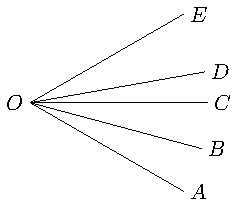
\includegraphics{pr1-4-7.pdf}
			\caption*{第 \ref{prac:1-4-7} 题}
		\end{minipage}%
		\begin{minipage}[b]{0.45\linewidth}\centering
		  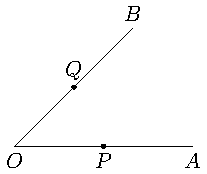
\includegraphics{pr1-4-8.pdf}
			\caption*{第 \ref{prac:1-4-8} 题}
		\end{minipage}
	\end{figurehere}
	\item 如果在射线 $OA$ 上依次取 5 个点,那么在射线 $OA$ 上(包括射线 $OA$ 在内)共有多少条射线?如果依次取 10 个点,100 个点那么在射线 $OA$ 上分别有多少条射线?如果在射线 $OA$ 上取 $n$ 个点,那么在射线 $OA$ 上又有多少条射线?
	\item 如果在直线 $\ell$ 上依次取 3 个点,那么直线 $\ell$ 上有多少条射线?如果取 100 个点,那么直线 $\ell$ 上有多少条射线?如果在 $\ell$ 上依次取 $n$ 个点,那么直线 $\ell$ 上有多少条射线?
\end{question}
\end{Practice}

\subsection{角度和旋转}
在前面我们说明了可以用以 $A$ 点为端点的一条射线来表示一个由 $A$ 点出发的方向。设射线 $AB$ 和 $AC$ 分别表示一个由 $A$ 点出发的两个方向,那么这两条射线所成的角也可以看作是一条以 $A$ 点为端点的射线,从 $AB$ 的位置沿着平面旋转到 $AC$ 的位置而成的图形。象度量线段 $\overline{PQ}$ 的长度就是度量表示 $P$、$Q$ 这两个位置之间的距离一样;度量射线 $AB$ 和 $AC$ 所表示的这两个方向之间的差别也就是度量这两条射线之间所夹的“角度”。而角度也就可以看成是旋转量了。下面采用旋转的观点对于角度的度量再作一初步的探讨:

\subsubsection{角度的大小}
\begin{figure}
	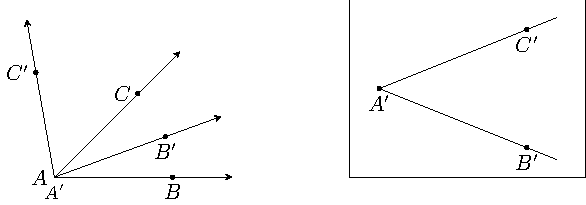
\includegraphics{1-29.pdf}
	\caption{}\label{fig:1-29}
\end{figure}

如\cref{fig:1-29} 所示,$\angle BAC$ 和 $\angle B'A'C'$ 分别是以 $A$ 和 $A'$ 为顶点的两个角,用一张透明的塑胶片,先把它盖在 $\angle B'A'C'$ 的上面,用笔把$\angle B'A'C'$ 复印到塑胶片上。然后把塑胶片移到 $\angle BAC$ 的上面,调整其位置使得顶点 $A$ 和顶点 $A'$ 相重合;再用一个针插在 $A$、$A'$ 点之上,这样,塑胶片仍然可以绕着针尖所插的 $A'$ 点旋转,但是 $A$、$A'$ 点依然确保重合。适当旋转可以使得两个角的边 $AB$ 和 $A'B'$ 重合,而且“角区”位于相重边的同侧(\cref{fig:1-30})。
\begin{figure}
	\begin{minipage}[b]{0.48\linewidth}
    \centering
		\includegraphics{1-30.pdf}
    \caption{}\label{fig:1-30}
  \end{minipage}
  \begin{minipage}[b]{0.48\linewidth}
    \centering
    \includegraphics{1-31.pdf}
    \caption{}\label{fig:1-31}
  \end{minipage}
\end{figure}


这样,两角之间有下列三种可能的位置关系:
\begin{itemize}
	\item 它们的另一边也重合,那么就说这两个角相等,记作 $\angle B'A'C'=\angle BAC$;
	\item $A'C'$ 落在 $\angle BAC$ 的内部,那么就说 $\angle B'A'C'$ 小于 $\angle BAC$,记作 $\angle B'A'C'<\angle BAC$;
	\item $A'C'$ 落在 $\angle BAC$ 的外部,那么就说 $\angle B'A'C'$ 大于 $\angle BAC$,记作 $\angle B'A'C'>\angle BAC$。
\end{itemize}

\subsubsection{两角的相加}
如\cref{fig:1-31} 所示,$\angle BAC$ 和 $\angle CAD$ 两个角的顶点相同,有一条边相重合(即射线 $AC$),而且两者的角区分居于公共边的两侧,就说 $\angle BAD$ 为 $\angle BAC$ 和 $\angle CAD$ 之和,即 $\angle BAD=\angle BAC+\angle CAD$。这时由等式的性质,又可知 $\angle BAC=\angle BAD-\angle CAD$,$\angle CAD=\angle BAD-\angle BAC$。

当两个角相加后是一个平角时,就说这两个角\Concept{互为补角},其中一个角叫做另一个角的补角。简称为\Concept{互补}(\cref{fig:1-32a})。一个角如果和它的补角相等,这个角叫做\Concept{直角}(\cref{fig:1-32b})。

\begin{figure}
	\begin{minipage}[b]{0.45\linewidth}\centering
	  \includegraphics{1-32a.pdf}
		\subcaption{}\label{fig:1-32a}
	\end{minipage}
	\begin{minipage}[b]{0.45\linewidth}\centering
	  \includegraphics{1-32b.pdf}
		\subcaption{}\label{fig:1-32b}
	\end{minipage}
	\caption{}\label{fig:1-32}
\end{figure}

小于直角的角叫做\Concept{锐角},大于直角小于平角的角叫做\Concept{钝角}。如\cref{fig:1-33} 所示,$\angle AOB$ 为锐角,$\angle CPD$ 为钝角。
\begin{figure}
	\begin{minipage}[b]{0.45\linewidth}\centering
		\includegraphics{1-33a.pdf}
		\subcaption{}\label{fig:1-33a}
	\end{minipage}
	\begin{minipage}[b]{0.45\linewidth}\centering
		\includegraphics{1-33b.pdf}
		\subcaption{}\label{fig:1-33b}
	\end{minipage}
	\caption{}\label{fig:1-33}
\end{figure}

如果两个角相加的和等于直角,这两角叫做互为\Concept{余角}。其中一个角叫做另一个角的余角。例如\cref{fig:1-34} 中的 $\angle\alpha+\angle\beta=$ 直角,则$\angle\alpha$、$\angle\beta$ 互为余角。

\begin{figure}
	\includegraphics{1-34.pdf}
	\caption{}\label{fig:1-34}
\end{figure}

\subsubsection{角的度量与量角器}
角的度量和线段的度量的做法基本上是相同的。也是先取定一个角度单位,然后用这个单位,或把它适当等分所得的分单位去和一个要量的角来比较大小。常用的单位是把一个平角分成 180 等份,其中一份叫做 1 度;再把 1 度分成 60 等份,其中一份叫做 1 分;再把 1 分分成 60 等份,其中一份叫做 1 秒。常用的符号是在数字的右上角上标以“\unit{\degree}”表示度,“\unit{\arcminute}”表示分,“\unit{\arcsecond}”表示秒。例如:35 度 12 分 30 秒就写成 \ang{35;12;30}。

平角$=\ang{180}$,平角的二等分角(即平角的一半)就是直角,直角$=\ang{90}$。四个直角相加得一周角,周角$=\ang{360}$。

\begin{figure}
  \includegraphics{1-35.pdf}
	\caption{}\label{fig:1-35}
\end{figure}

度量长度的常用工具是刻有等分刻度的直尺,相应地度量角度的常用工具是\cref{fig:1-35} 所示的量角器。量角器是一个具有 180 个等分刻度的半圆形塑胶板,当我们要去量一个给定的角的角度时,先把顶点和这个半圆板的圆心叠合,然后使得直径和角的一边相重合;那么角的另一边通过半圆的位置的刻度就是所量角度的近似值。如\cref{fig:1-36} 中的 $\angle BAC$,$AB$ 与 \ang{0} 线重合,$AC$ 恰好落在 \ang{40} 的刻度上,所以$\angle BAC=\ang{40}$。

\begin{figure}
	\includegraphics{1-36.pdf}
	\caption{}\label{fig:1-36}
\end{figure}

\begin{example}
	求 \ang{30;19;21} 与 \ang{18;40;42} 的和。
\end{example}

\begin{solution}
\[ \ang{30;19;21}+\ang{18;40;42}=\ang{48;59;63} =\ang{49;;3}\]
\end{solution}

\begin{example}
	把 \ang{3.62} 化成度、分、秒。
\end{example}

\begin{solution}
$\because\quad 1^{\circ}=60',\qquad \therefore\quad 0.62^{\circ}=60'\times 0.62=37.2'$

$\because\quad 1'=60'',\qquad \therefore\quad 0.2'=60''\times 0.2=12''$

$\therefore\quad \ang{3.62}=\ang{3;37;12}$
\end{solution}

\begin{example}
	把 \ang{15;18;15} 化为度。
\end{example}


\begin{solution}
	先把 \ang{;;15} 化为分:
\[\frac{\ang{;;15}}{\ang{;;60}}=\ang{;0.25;}\]
$\therefore\quad \ang{;18;15}=\ang{;18.25;}$。
再把 \ang{;18.25;} 化为度:
\[\frac{\ang{;18.25;}}{\ang{;60;}}\approx \ang{0.304}\]
$\therefore\quad \ang{15;18;15}\approx \ang{15.304}$。
\end{solution}

\subsubsection{对顶角相等和两条直线互相垂直}

如\cref{fig:1-37} 所示 直线 $AB$ 和 $CD$ 相交于 $O$ 点,这时,$\angle AOC$ 和 $\angle BOD$ 中 $OA$ 和 $OB$,$OC$ 和 $OD$ 都互为反向延长线。象这样,一个角的两边分别是另一个角的两边的反向延长线时,我们就称这两个角为\Concept{对顶角}。

\begin{figure}
	\includegraphics{1-37.pdf}
	\caption{}\label{fig:1-37}
\end{figure}

如果两个角是对顶角,那么它们之间有什么关系呢?由\cref{fig:1-37} 可知,$\angle AOC$ 和 $\angle AOD$ 互为补角,即 $\angle AOC+\angle AOD=\ang{180}$;$\angle BOD$ 和 $\angle AOD$ 也互为补角,即 $\angle BOD+\angle AOD=\ang{180}$,因而  $\angle AOC+\angle AOD=\angle BOD+\angle AOD$,所以,$\angle AOC=\angle BOD$。

总结上述事实就成为下述性质:\emph{对顶角相等}。

\begin{example}
如果两条直线 $AB$、$CD$ 相交于 $O$ 点(\cref{fig:1-37}),$\angle AOC=\ang{40}$,求 $\angle BOD$,$\angle AOD$,$\angle COB$ 的度数。
\end{example}

\begin{solution}
两条直线 $AB$、$CD$ 相交于 $O$ 点

$\therefore\quad \angle AOC$ 和 $\angle BOD$ 是对顶角,$\therefore\quad \angle AOC=\angle BOD$(对顶角相等)。

$\because\quad \angle AOC=\ang{40}$

$\therefore\quad \angle BOD=\ang{40}$。

又:$\angle AOC+\angle AOD=\ang{180}$,

$\therefore\quad \angle AOD=\ang{180}-\angle AOC=\ang{180}-\ang{40}=\ang{140}$。

$\because\quad \angle AOD=\angle COB$(对顶角相等)

$\therefore\quad \angle COB=\ang{140}$
\end{solution}

由于两条直线相交得出四个角,根据对顶角的概念可知,这四个角分为两双对顶角,当然每双对顶角都是相等的。并且不难看出,如果两条直线相交得出的四个角中,有一个是直角,那么其余的三个角也都是直角。

\medskip\noindent
\begin{minipage}{0.65\linewidth}\parindent2em
当两条直线相交成直角时,这两条直线就叫做\Concept{互相垂直}。其中一条叫做另一条的垂线,交点叫做\Concept{垂足}。如\cref{fig:1-38} 所示 $\ell_1$ 和 $\ell_2$ 互相垂直,$O$ 是它们的垂足,记作 $\ell_1\perp \ell_2$ 于 $O$ 点。符号“$\perp$”读作“垂直于”。

因为三角板中有一个角是直角,所以可以用三角板来画垂线。
\end{minipage}%
\begin{minipage}{0.35\linewidth}\centering
\begin{figurehere}
  \includegraphics{1-38.pdf}
	\caption{}\label{fig:1-38}
\end{figurehere}
\end{minipage}

\begin{example}
	过已知点 $A$,画已知直线 $\ell$ 的垂线。
\end{example}

\begin{solution}
\begin{enumerate}
	\item $A$ 点在直线 $\ell$ 上
	\item $A$ 点在直线 $\ell$ 外
\end{enumerate}
过 $A$ 点画直线 $\ell$ 的垂线的方法如\cref{fig:1-39} 所示。

\begin{figure}
	\begin{minipage}[b]{0.48\linewidth}
		\centering
		\includegraphics{1-39a.pdf}
		\caption*{过直线 $\ell$ 上一点 $A$ 划 $\ell$ 的垂线}
	\end{minipage}
	\begin{minipage}[b]{0.48\linewidth}
		\centering
		\includegraphics{1-39b.pdf}
		\caption*{过直线 $\ell$ 外一点 $A$ 划 $\ell$ 的垂线}
	\end{minipage}
	\caption{}\label{fig:1-39}
\end{figure}
\end{solution}

\begin{enumerate}[label=问题~\arabic*,leftmargin=1em,font=\bfseries]
	\item 实际画一画,过已知直线上或直线外一点,画这条直线的垂线能画几条?
	\item 如\cref{fig:1-40}, $P$ 点是直线 $AB$ 外一点,$PC\perp AB$ 于 $C$ 点,$D$、$E$ 都是直线 $AB$ 上的点,连结 $\overline{PD}$、$\overline{PE}$,量一量 $\overline{PC}$、$\overline{PD}$、$\overline{PE}$ 哪一条最短?
\end{enumerate}

\medskip
通过上面的实践,我们可以得出垂线的下列性质:
\begin{Theorem}{性质}
	\begin{enumerate}
	\item 过一点作一条直线的垂线,只能作一条。
	\item 从直线外一点和这条直线上各点所引的线段中,垂直线段最短。
\end{enumerate}
\end{Theorem}

\begin{figure}
	\begin{minipage}[b]{0.48\linewidth}
		\centering
		\includegraphics{1-40.pdf}
		\caption{}\label{fig:1-40}
	\end{minipage}
	\begin{minipage}[b]{0.48\linewidth}
		\centering
		\includegraphics{1-41.pdf}
	\caption{}\label{fig:1-41}
	\end{minipage}
\end{figure}

过直线外一点画这条直线的垂线,这点到垂足间的线段的长度叫做这点到这条直线的\Concept{距离}。

例如,从直线 $\ell$ 外一点 $A$,向直线 $\ell$ 画垂线,设垂足为 $B$,那么$\overline{AB}$ 的长度就是点 $A$ 到直线 $\ell$ 的距离(\cref{fig:1-41})。

\subsubsection{三角形的内角和}

我们观察手中的一副三角板(\cref{fig:1-42}),它们的大小形状都不相同;其中一个三角板的三个角和另一个三角板的三个角之间的大小,虽然都有一个直角,但其余的两对角的大小是不一样的,如果我们把每个三角形三个角的大小各自加起来:
\[\begin{split}
\ang{90}+\ang{45}+\ang{45}&=\ang{180}\\
\ang{90}+\ang{60}+\ang{30}&=\ang{180}	
\end{split}\]
结果发现两个三角板的三个角的和都相同,都等于 \ang{180}。

\begin{figure}
  \includegraphics{1-42.pdf}
	\caption{}\label{fig:1-42}
\end{figure}

这样,我们自然地会想到:任何一个三角形的三个角的和等于多少度?是否也等于 \ang{180}?

同学们在纸上任意画两个三角形,形状、大小都不要一样,但要认真仔细地画,边要画得直,笔道要越细越好。然后用量角器去量它们的各角,把每一个三角形的三个角的度数加起来,如果得到的两个结果相差很大,就再仔细地量一量、算一算,如果得到的两个结果相差极为微小,而且都极其接近 \ang{180}, 那么我们又会想到:如果在量的过程中没出现误差,是否任何一个三角形的三个角的和都等于 \ang{180}?

带着这个问题,我们不妨这样来设想,因为 \ang{180} 角即平角,它的两边合成一条直线,如果三角形三个角的大小的和等于 \ang{180},那么这三个角拼合起来就应该得到一个平角。因此我们可以按照这个设想,再来检验三角形三个角的和是否为一个平角,即 \ang{180}角。

先用硬纸板仔细地剪出一个三角形(如\cref{fig:1-43a}),然后在桌上放一把直尺(\cref{fig:1-43a});再沿着\cref{fig:1-43a} 中任意画的虚线把三个角(记作$\angle 1$,$\angle 2$,$\angle 3$)剪下来;最后按\cref{fig:1-43b} 所示,把 $\angle 1$,$\angle 2$,$\angle 3$ 拼合起来放在直尺的边上,结果,作为 $\angle 1$,$\angle 2$,$\angle 3$ 之和的角的两边恰好和直尺的边密合。

\begin{figure}
	\begin{minipage}[b]{0.45\linewidth}\centering
    \includegraphics{1-43a.pdf}
		\subcaption{}\label{fig:1-43a}
	\end{minipage}
	\begin{minipage}[b]{0.45\linewidth}\centering
    \includegraphics{1-43b.pdf}
		\subcaption{}\label{fig:1-43b}
	\end{minipage}
	\caption{}\label{fig:1-43}
\end{figure}

通过以上实践,我们便总结出实验的结果,这就是:

\begin{Theorem}{性质}
三角形的三个角的和是 \ang{180}。	
\end{Theorem}

\begin{example}
已知如\cref{fig:1-44}, $\triangle ABC$ 中,$\angle A=\ang{55}$,$\angle B=\ang{48}$。$BD\perp AC$于 $D $点。求 $\angle DBC$ 的度数。
\end{example}
\par\medskip\noindent
\begin{minipage}{0.7\linewidth}
	\begin{solution}
		$\because\,\,$ 三角形的三个角之和是 \ang{180}
		
		$\therefore\,\, \angle A+\angle ABC+\angle C=\ang{180}$
		
		$\therefore\,\, \angle C=\ang{180}-\angle A-\angle ABC
		=\ang{180}-\ang{55}-\ang{48}=\ang{77}$。
		
		又 $\because\,\, BD\perp AC$ 于 $D$ 点,
		
		$\therefore\,\, \angle BDC=\ang{90} $
		
		$\therefore\,\, \angle DBC=\ang{180}-\angle C-\angle BDC
		=\ang{180}-\ang{77}-\ang{90}=\ang{13}$。
	\end{solution}
\end{minipage}%
\begin{minipage}{0.3\linewidth}\centering
  \begin{figurehere}
		\includegraphics{1-44.pdf}
		\caption{}\label{fig:1-44}
	\end{figurehere}
\end{minipage}

\begin{Practice}
\begin{question}
	\item\label{prac:1-5-1} 看图在各题的(\qquad)中填入适当的角:
	\begin{tasks}(2)
		\task $\angle ABD=\angle ABC+(\qquad )$
		\task $\angle CBE-\angle DBE=(\qquad)$
		\task* $\angle ABE-\angle CBD=\angle ABC+(\qquad)$
	\end{tasks}
	\begin{figurehere}
		\begin{minipage}[b]{0.48\linewidth}
			\centering
			\includegraphics{pr1-5-1.pdf}
			\caption*{第 \ref{prac:1-5-1} 题}
		\end{minipage}
		\begin{minipage}[b]{0.48\linewidth}
			\centering
			\includegraphics{pr1-5-4.pdf}
			\caption*{第 \ref{prac:1-5-4} 题}
		\end{minipage}
	\end{figurehere}
	\item\label{prac:1-5-2} 什么是平角、直角、锐角、钝角?指出下列图中的锐角、直角和钝角。
	\begin{figurehere}
		\begin{minipage}{\linewidth}\centering
			\includegraphics{pr1-5-2.pdf}
			\caption*{第 \ref{prac:1-5-2} 题}
		\end{minipage}
	\end{figurehere}
	\item 分别指出,时针和分针在下列哪个时间组成锐角、钝角、直角和平角。
	\begin{tasks}(3)
		\task 4 点
		\task 6 点
		\task 9 点
		\task 1 点 30 分
		\task 2 点 5分
	\end{tasks}
	\item\label{prac:1-5-4} 什么叫两个角互补?如果已知 $\angle AOB$,试画出 $\angle AOB$ 的补角。
	\item 什么叫两个角互为余角?如果 $\angle \alpha+\angle \beta=$ 直角,那么说“$\angle \alpha$ 是余角”,“$\angle\beta$ 是余角”,对吗?怎样才是正确的说法?
	\item\label{prac:1-5-6} 用量角器分别量出下列各角的度数。
	\begin{figurehere}
		\begin{minipage}{\linewidth}\centering
			\includegraphics{pr1-5-6.pdf}
			\caption*{第 \ref{prac:1-5-6} 题}
		\end{minipage}
	\end{figurehere}
	\item 用量角器分别画出 \ang{45},\ang{72},\ang{90},\ang{134} 的角。
	\item\label{prac:1-5-8} 什么叫对顶角?下列各图中有没有对顶角?如果有,把它们写出来。
	\begin{figurehere}
		\begin{minipage}{\linewidth}
		\begin{minipage}[b]{0.3\linewidth}\centering
			\includegraphics{pr1-5-8a.pdf}
			\subcaption{}
		\end{minipage}%
		\begin{minipage}[b]{0.3\linewidth}\centering
			\includegraphics{pr1-5-8b.pdf}
			\subcaption{}
		\end{minipage}%
		\begin{minipage}[b]{0.4\linewidth}\centering
			\includegraphics{pr1-5-8c.pdf}
			\subcaption{}
		\end{minipage}
		\caption*{第 \ref{prac:1-5-8} 题}
		\end{minipage}
	\end{figurehere}
	\item\label{prac:1-5-9} 已知(如图)直线 $AB$ 和 $CD$ 相交于 $O$ 点,$\angle AOC=\ang{50;20;}$,求 $\angle BOD$、$\angle COB$ 和 $\angle AOD$。
	\item 计算下列各题:
	\begin{tasks}(2)
		\task $\ang{3;25;18}+\ang{24;39;24}$
		\task $\ang{64;27;15}-\ang{28;37;35}$
	\end{tasks}
	\begin{figurehere}
		\begin{minipage}[b]{0.48\linewidth}
			\centering
			\includegraphics{pr1-5-9.pdf}
			\caption*{第 \ref{prac:1-5-9} 题}
		\end{minipage}
		\begin{minipage}[b]{0.48\linewidth}
			\centering
			\includegraphics{pr1-5-16.pdf}
			\caption*{第 \ref{prac:1-5-16} 题}
			\end{minipage}
	\end{figurehere}
	\item 化下列单名数为复名数(度、分、秒)。
	\[1.25^{\circ};\quad 0.8^{\circ};\quad 3.21^{\circ};\quad (1\frac{1}{2})^{\circ};\quad (2\frac{1}{3})^{\circ}\]
	\item 化下列复名数为单名数(度)。
	\[\ang{5;30;};\quad \ang{12;36;12};\quad \ang{38;4;5}\]
	\item 求 \ang{23.26}、\ang{15;25;15} 的角的补角的大小。
	\item 求 \ang{48;15;}、\ang{72.9} 的角的余角的大小。
	\item 什么是两点间的距离?什么是直线外一点到这条直线的距离?
	\item\label{prac:1-5-16} 已知:$P$ 在直线 $\ell$ 上,$Q$ 在直线 $m$ 上,试量出:
	\begin{tasks}(2)
		\task $P$、$Q$ 两点间的距离;
		\task $P$ 到直线 $m$ 的距离;
		\task $Q$ 点到直线 $\ell$ 的距离。
	\end{tasks}
	\item\label{prac:1-5-17} 已知如图,用三角板:
	\begin{tasks}(2)
		\task 过 $A$ 点画出直线 $BC$ 的垂线;
		\task 过 $B$ 点画出直线 $AC$ 的垂线;
		\task 过 $C$ 点画出直线 $AB$ 的垂线。
	\end{tasks}
	\begin{figurehere}
		\begin{minipage}[b]{0.48\linewidth}
			\centering
			\includegraphics{pr1-5-17.pdf}
			\caption*{第 \ref{prac:1-5-17} 题}
		\end{minipage}
		\begin{minipage}[b]{0.48\linewidth}
			\centering
			\includegraphics{pr1-5-19.pdf}
			\caption*{第 \ref{prac:1-5-19} 题}
		\end{minipage}
	\end{figurehere}
	\item 已知$\triangle ABC$中,$\angle A=\ang{70}$, $\angle B=\ang{60}$,求 $\angle C$。
	\item\label{prac:1-5-19} 如图,$\angle 1=\ang{35}$,$\angle 2=\ang{78}$,求 $\angle 3$ 的大小,自 $\angle 3$ 的顶点画一条射线和 $\angle 1$ 的一条边相交,并且使 $\angle 4=\ang{16}$。

	问:$\angle 5$比$\angle 2$少多少度?
	\item 怎样从“三角形三个内角和等于 \ang{180}”推算出四边形的四个内角的和,五边形五个内角的和,六边形六个内角的和各等于多少度?
	\item\label{prac:1-5-21} 如果分别延长 $\triangle ABC$ 的三边 $AB$、$BC$、$CA$ 得到 $\angle 1$、$\angle 2$ 和 $\angle 3$,那么 $\angle 1+\angle 2+\angle 3=?$
	\item\label{prac:1-5-22} 如果顺次延长四边形 $ABCD$ 的各边,得到 $\angle 1$、$\angle 2$、$\angle 3$ 和 $\angle 4$,那么,请你根据第 \ref{prac:1-5-21} 题的计算结果猜想一下这四个角之和可能是多少度?然后再计算一下 $\angle 1+\angle 2+\angle 3+\angle 4=?$ 来验证一下你的猜想是否正确。
	\begin{figurehere}
		\begin{minipage}[b]{0.48\linewidth}
			\centering
			\includegraphics{pr1-5-21.pdf}
			\caption*{第 \ref{prac:1-5-21} 题}
		\end{minipage}
		\begin{minipage}[b]{0.48\linewidth}
			\centering
			\includegraphics{pr1-5-22.pdf}
			\caption*{第 \ref{prac:1-5-22} 题}
			\end{minipage}
	\end{figurehere}
\end{question}
\end{Practice}

\subsection{角度和平行}
在前面的讨论中,我们已经明确了沿着一个固定方向一直走,所经过的路线就是一条射线。如\cref{fig:1-45} 所示,射线 $AB$ 和射线 $A'B'$ 分别表示起点为 $A$ 和 $A'$ 的两个方向。连结 $A$、$A'$ 再延长得射线 $AA'$,于是射线 $AC$ 和射线 $A'C'$ 是相同的两个方向;$\angle CAB$ 表示射线 $AB$ 和 $AC$ 这两个方向的差别,$\angle C'A'B'$ 表示射线 $A'B'$ 和 $A'C'$ 这两个方向的差别。如果 $\angle CAB=\angle C'A'B'$,显然射线 $AB$ 和 $A'B'$ 的方向就是相同的。

\begin{figure}
	\begin{minipage}[b]{0.48\linewidth}
		\centering
    \includegraphics{1-45.pdf}
		\caption{}\label{fig:1-45}
	\end{minipage}
	\begin{minipage}[b]{0.48\linewidth}
		\centering
		\includegraphics{1-46.pdf}
		\caption{}\label{fig:1-46}
	\end{minipage}
\end{figure}


我们把 $\angle CAB$ 和 $\angle C'A'B'$ 这样位置的角叫做\Concept{同位角}。如\cref{fig:1-46} 所示。

连结同一平面内的射线 $AB$ 和 $A'B'$ 的端点 $A$、$A'$ 后,如果得到的同位角相等(\cref{fig:1-45})即 $\angle CAB=\angle C'A'B'$,我们就说射线 $AB$ 和 $A'B'$ 互相平行。同样地,如果同一平面内的两条直线 $\ell$ 和 $\ell'$ 被另一条直线 $AA'$ 截出的同位角相等(\cref{fig:1-47}),我们就说直线 $\ell$ 和 $\ell'$ \Concept{互相平行}。记作 $\ell\parallel \ell'$。

\begin{figure}
    \begin{minipage}[b]{0.48\linewidth}
    	\centering
			\includegraphics{1-47.pdf}
    	\caption{}\label{fig:1-47}
    \end{minipage}
    \begin{minipage}[b]{0.48\linewidth}
    	\centering
			\includegraphics{1-48.pdf}
    \caption{}\label{fig:1-48}
  \end{minipage}
\end{figure}

\begin{example}
在纸上画一条直线记为 $\ell$,在 $\ell$ 外任意取一点 $A'$(\cref{fig:1-48}),怎样在纸上过 $A'$ 画一条直线和 $\ell$ 平行?
\end{example}

\begin{solution}
根据同位角相等,两条直线就平行,这一平行线的意义,我们在直线 $\ell$ 上先取一点$A$,再连结出直线 $AA'$,然后量出 $\angle 1$ 的大小,并用量角器划出 $\angle 2=\angle 1$,这时 $\angle 2$ 的另一条边所在直线 $\ell'$ 就是 $\ell$ 的平行线。如果在 $\ell$ 上另取一点 $B$,仍用画同位角 $\angle 4=\angle 3$ 的方法画出过点$A'$ 和直线 $\ell$ 平行的直线,结果这条直线仍然是 $\ell'$。

同样地,如果在直线 $\ell$ 上另取点 $C$、$D$、……(图中没有画出)而后分别按上面的方法画出过点 $A'$ 和 $\ell$ 的平行线,结果这条直线还是 $\ell'$。

通过画图,我们得到:
\begin{Theorem}{性质}
	过已知直线 $\ell$ 外的一点 $P$ 只有一条直线和 $\ell'$ 平行。
\end{Theorem}
\end{solution}

\begin{example}
	教室里的长方形黑板的对边是不是平行线?为什么(\cref{fig:1-49})?
\end{example}

\smallskip\noindent
\begin{minipage}{0.5\linewidth}\parindent2em
	\begin{solution}
		由小学数学课中我们已知长方形的各角都是直角,如图,长方形的 $\angle 1$、$\angle 2$、$\angle 3$、$\angle 4$ 都是直角。
		
		因为 $\angle 1'$ 是 $\angle 1$ 的补角,所以 $\angle 1'$ 也是直角,于是同位角 $\angle 1'=\angle 2$,因此长方形的对边 $a\parallel a'$。 
		
		同样,同位角 $\angle 3'=\angle 2$,因此另一对边 $b\parallel b'$。 
	\end{solution}
\end{minipage}
\begin{minipage}{0.45\linewidth}\centering
	\begin{figurehere}\quad
		\includegraphics{1-49.pdf}
		\caption{}\label{fig:1-49}
	\end{figurehere}
\end{minipage}

\medskip 
我们学习了平行线的意义之后,进一步考虑平面上两条直线 $\ell$,$m$ 有几种可能的位置关系呢?参看\cref{fig:1-50},同学们自己归纳出结论。
\begin{figure}
	\includegraphics{1-50.pdf}
	\caption{}\label{fig:1-50}
\end{figure}

\begin{Practice}
\begin{question}
	\item\label{prac:1-6-1} 如图,在同一平面内,直线 $m$ 和 $\ell$ 垂直于 $A$ 点,直线 $\ell$ 和 $m$ 垂线于 $A'$ 点,直线 $\ell$ 和 $\ell'$ 平行吗?为什么?
	\item\label{prac:1-6-2} 如图,先把三角板的一边 $a$ 和直线 $\ell$ 密合;再用直尺和三角板的另一边 $b$ 密合;固定直尺,推动三角板使$b$总和直尺密合,当 $a$ 过 $P$ 点时,沿 $a$ 画直线 $\ell'$,那么 $\ell'\parallel \ell$。为什么?
	\begin{figurehere}
		\begin{minipage}[b]{0.48\linewidth}
			\centering
			\includegraphics{pr1-6-1.pdf}
			\caption*{第 \ref{prac:1-6-1} 题}
		\end{minipage}
		\begin{minipage}[b]{0.48\linewidth}
			\centering
			\includegraphics{pr1-6-2.pdf}
			\caption*{第 \ref{prac:1-6-2} 题}
		\end{minipage}
	\end{figurehere}
\item 已知直线 $AB$ 外一点 $C$,过 $C$ 点划一条直线和 $AB$ 平行。
\item 两条平行直线是否可以确定一个平面?
\end{question}
\end{Practice}

\begin{Exercise}
\begin{question}
	\item 用度、分、秒表示下列各角:
	\begin{tasks}(3)
		\task $\dfrac{1}{2}$直角
		\task $\dfrac{1}{4}$直角
		\task $1\dfrac{1}{4}$直角
		\task \ang{48.45}
		\task \ang{58.19}
		\task \ang{;;384600}
	\end{tasks}
	\item 计算下列式子:
	\begin{tasks}(2)
		\task $\ang{38;24;}+\ang{54;43;}$
		\task $\ang{180}-\ang{99;48;}$
		\task $52^{\circ}13'-27^{\circ}58'$
		\task $24^{\circ}3'\times 15$
		\task $200^{\circ}45'\div 5$
		\task $\ang{144}\div \ang{12}$
		\task $\ang{18;33;} \div 4$
		\task $\ang{315;5;}\div \ang{14;8;}$
	\end{tasks}
	\item\label{exec:1-2-3} 检验图中两条直线 $OA$,$O'A'$ 是否平行。
	\begin{figurehere}
		\begin{minipage}[b]{0.48\linewidth}
			\centering
			\includegraphics{ex1-2-3.pdf}
			\caption*{第 \ref{exec:1-2-3} 题}
		\end{minipage}
		\begin{minipage}[b]{0.48\linewidth}
			\centering
			\includegraphics{ex1-2-4.pdf}
			\caption*{第 \ref{exec:1-2-4} 题}
		\end{minipage}
	\end{figurehere}
	\item\label{exec:1-2-4} 检验图中的两条直线是否垂直。
	\item 回答下列问题:
	\begin{tasks}
		\task 钝角与锐角的差一定比直角大吗?举例说明。
		\task 两个锐角的和会不会大于直角?会不会大于或等于平角?
		\task 两个钝角的和会不会大于或等于一个周角。
	\end{tasks}
	\item 下面的说法对不对?为什么?
	\begin{tasks}(2)
		\task 锐角的余角是锐角。
		\task 锐角的补角是锐角。
		\task 直角的补角是直角。
		\task 两个锐角不能互为补角。
		\task! 两个角如果互余,这两个角都是锐角。
		\task! 一个锐角和一个钝角一定互为补角。
		\task! 两个角如果互补,一定是一个角为锐角一个角为钝角。
		\task! 一个锐角加上一个锐角,还是一个锐角。
		\task! 一个钝角减去一个比它小的钝角,差是锐角。
	\end{tasks}
	\item 一个角的补角是它的 3 倍,求这个角的度数。
	\item 一个角的余角是它的 3 倍,求这个角的度数。
	\item 一个角是它的补角的 4 倍,求这个角是多少度?
	\item 两个角的度数比为 $7:2$,它们的差是 \ang{50},求这两个角的度数。
	\item 两条直线相交有一个角是 \ang{20},求其余各角。
	\item\label{exec:1-12} 已知 $AB$ 是直线,$O$ 点在 $AB$ 上,直线 $CO\perp DO$,那么 $\angle 1$ 与$\angle 2$ 互余吗?为什么?
	\item\label{exec:1-13} 如图,试:
	\begin{tasks}(2)
		\task 过 $B$ 点画直线 $AD$ 的垂线?
		\task 过 $D$ 点画直线 $BC$ 的垂线?
		\task 过 $O$ 点画直线 $BD$ 的垂线?
	\end{tasks}
	\begin{figurehere}
		\begin{minipage}[b]{0.48\linewidth}
			\centering
			% \includegraphics{ex1-12.pdf}
			\caption*{第 \ref{exec:1-12} 题}
		\end{minipage}
		\begin{minipage}[b]{0.48\linewidth}
			\centering
			% \includegraphics{ex1-13.pdf}
			\caption*{第 \ref{exec:1-13} 题}
		\end{minipage}
	\end{figurehere}
	\item 下面的说法对不对?说明理由。
	\begin{tasks}
		\task 可能有三个角都是锐角的三角形。
		\task 可能有二个角都是直角的三角形。
		\task 不可能有一个角是直角,另一个角是钝角的三角形。
		\task 可能有一个角是钝角,其余两个角都是锐角的三角形。
	\end{tasks}
\end{question}
\end{Exercise}

\section{全等和叠合}
\subsection{全等形}
两个形状和大小完全相同的图形,叫做全等形。如\cref{fig:1-51a} 中,三角形 \MyRoman{2} 和 \MyRoman{1} 面积的大小相等但形状不同; \MyRoman{3} 和 \MyRoman{1} 的形状相同但大小又不等; \MyRoman{4} 和 \MyRoman{1} 的形状和大小都不一样,只有 \MyRoman{5} 和 \MyRoman{1} 的形状和大小完全相同。三角形 \MyRoman{1} 和 \MyRoman{5} 是全等的。又如\cref{fig:1-51b} 中,三棱锥 \MyRoman{1}$'$ 和 \MyRoman{2}$'$ 形状相同但大小不等;\MyRoman{3}$'$ 和 \MyRoman{2}$'$ 体积的大小相等但形状又不同。只有 \MyRoman{4}$'$ 和 \MyRoman{2}$'$ 的形状和大小完全相同。三棱锥 \MyRoman{2}$'$ 和 \MyRoman{4}$'$ 是全等的。

\begin{figure}
  \begin{minipage}{\linewidth}\centering
		\includegraphics{1-51a.pdf}
		\subcaption{}\label{fig:1-51a}
	\end{minipage}
  \begin{minipage}{\linewidth}\centering
		\includegraphics{1-51b.pdf}
		\subcaption{}\label{fig:1-51b}
	\end{minipage}
	\caption{}\label{fig:1-51}
\end{figure}

我们用符号“$\cong$”表示全等。在图中就有:
\begin{center}
	三角形 \MyRoman{1} $\cong$ 三角形 \MyRoman{5};\qquad 三棱锥 \MyRoman{2}$'\cong$ 三棱锥 \MyRoman{4}$'$
\end{center}

对于平面上两个图形(简称平面图形),要看一看他们是否全等,实践检验的方法,常常是看它能否叠合。能叠合的就全等。

显然,两条线段 $\overline{AB}$ 和 $\overline{A'B'}$ 能叠合的唯一条件就是它们等长:$\overline{AB}=\overline{A'B'}$。

在角的度量的讨论中,我们实际就是用叠合来说明两个角的大小相等的意义的,这也就是说两个角 $\angle A$ 和 $\angle A'$ 能叠合的唯一条件就是它们的大小相等:$\angle A=\angle A'$。

如果 $\triangle ABC$ 和 $\triangle A'B'C'$ 全等(\cref{fig:1-52}),这就是说它们能叠合。因而他们的边和角便分别相等(也说全等形的对应边相等、对应角相等):
\begin{figure}
  \includegraphics{1-52.pdf}
	\caption{}\label{fig:1-52}
\end{figure}
\[\begin{split}
\overline{AB}=\overline{A''C''},&\quad \overline{BC}=\overline{B''C''},\quad \overline{CA}=\overline{B''A''}\\
\angle A=\angle A'',&\quad \angle B=\angle C'',\quad \angle C=\angle B''
\end{split}\]

\subsection{三角形全等的条件}
由上面对两个全等三角形的分析,知道了两个三角形如果全等,它们的对应边、对应角都分别相等。反过来说,如果两个三角形的各边对应相等,对应角也分别相等,那么这两个三角形便能叠合,它们就是全等三角形。

下面我们来研究两个三角形的全等条件。

\begin{enumerate}
	\item 如\cref{fig:1-53} 中,$\angle A=\angle A'$,$\overline{AB}=\overline{A'B'}$,$\overline{AC}=\overline{A'C'}$。那么可以使$\overline{A'B'}$ 叠合在 $\overline{AB}$ 上,从而 $\angle A'$ 可以和 $\angle A$ 叠合,同时 $\overline{A'C'}$ 也就叠合在 $\overline{AC}$ 上了。这样一来,由于点 $B'$ 落在点 $B$ 上,点 $C'$ 落在点 $C$ 上,那么根据“两点只确定一条直线”这个基本性质,直线 $B'C'$ 便叠合在直线 $BC$ 上,自然 $\overline{B'C'}$ 和 $\overline{BC}$ 也就叠合在一起,于是 $\triangle ABC$ 和 $\triangle A'B'C'$ 便完全叠合,它们也就全等了。
	\begin{figure}
		\includegraphics{1-53.pdf}
		\caption{}\label{fig:1-53}
	\end{figure}

	由此可见,检验两个三角形是否全等时,不必分别的检验它们的各边是否对应相等、各对应角是否相等,而是检验出两条边和所夹的角分别相等就可判定这两个三角形全等了。这种判定两个三角形全等的条件,记作(SAS)条件。
	\item 与此相仿,如\cref{fig:1-53} 中 $\angle A=\angle A'$,$\overline{AB}=\overline{A'B'}$,$\angle B=\angle B'$,也可以先使 $\overline{A'B'}$ 叠合在 $\overline{AB}$ 上,再让 $\triangle A'B'C'$ 落在 $\triangle ABC$ 所在平面上,因为 $\angle A'=\angle A$,$\angle B'=\angle B$,所以 $\angle A'$ 和 $\angle A$,$\angle B'$ 和 $\angle B$ 分别叠合;这样,直线 $A'B'$ 和 $AC$,$B'C'$ 和 $BC$ 也就分别叠合了,由于“两条直线相交只有一个交点”。因此,点 $A'$ 必落在点 $A$ 上,于是 $\triangle A'B'C'$ 和 $\triangle ABC$ 就完全叠合了,因此它们全等。这就是说两角和夹边对应相等的两个三角形全等。这种判定两个三角形全等的条件,记作(ASA)条件。
	\item 再有,如果一个三角形的三条边的长度确定了,通过观察和实验我们可以发现这个三角形的形状和大小就不会改变了(\cref{fig:1-54a})。而一个四边形如果四条边的长度确定了,它的形状和大小却是可以改变的(\cref{fig:1-54b})。我们把三角形的这种特性叫做三角形的\Concept{稳定性}。
	\begin{figure}
		\begin{minipage}[b]{0.45\linewidth}\centering
			\includegraphics{1-54a.pdf}
			\subcaption{}\label{fig:1-54a}
		\end{minipage}
		\begin{minipage}[b]{0.45\linewidth}\centering
			\includegraphics{1-54b.pdf}
			\subcaption{}\label{fig:1-54b}
		\end{minipage}
		\caption{}\label{fig:1-54}
	\end{figure}

	这样,一个三角形 $ABC$ 的三边和另一个三角形 $A'B'C'$ 的三边如果对应地相等,即 $\overline{AB}=\overline{A'B'}$,$\overline{BC}=\overline{B'C'}$,$\overline{AC}=\overline{A'C'}$,那么由三角形的稳定性,这两个三角形的对应角也必相等。即 $\angle A=\angle A'$,$\angle B=\angle B'$,$\angle C=\angle C'$。因此,这两个三角形就全等。这种判定三角形全等的条件,记作(SSS)条件。
\end{enumerate}

\begin{example}
  在\cref{fig:1-55} 中,如果已知 $\overline{AB}=\overline{DC}$,$\overline{AC}=\overline{DB}$,$\triangle ABC$ 和 $\triangle DCB$ 全等吗?为什么?
\end{example}

\medskip\noindent
\begin{minipage}{0.6\linewidth}
	\begin{solution}
		在 $\triangle ABC$ 和 $\triangle DCB$ 中,由于:
		\begin{align*}
			\overline{AB}&=\overline{DC}  \tag{已知}\\
			\overline{AC}&=\overline{DB} \tag{已知}\\
			\overline{BC}&=\overline{BC}  \tag{公共边}	
		\end{align*}
		$\therefore\quad \triangle ABC\cong \triangle DCB$(SSS)。
	\end{solution}
\end{minipage}%
\begin{minipage}{0.4\linewidth}\centering
  \begin{figurehere}
		\includegraphics{1-55.pdf}
		\caption{}\label{fig:1-55}
	\end{figurehere}
\end{minipage}

\begin{example}
在\cref{fig:1-56} 中已知 $\overline{AD}=\overline{AE}$,$\overline{AB}=\overline{AC}$,那么 $\triangle ABE$ 和 $\triangle ACD$ 全等吗?为什么?
\end{example}

\noindent
\begin{minipage}{0.6\linewidth}
	\begin{solution}
		在$\triangle ABE$和$\triangle ACD$中,由于:
		\begin{align*}
			\overline{AD}&=\overline{AE}  \tag{已知}\\
			\overline{AB}&=\overline{AC} \tag{已知}\\
			\angle A&=\angle A  \tag{公共角}	
		\end{align*}
	$\therefore\quad \triangle ABE\cong \triangle ACD$(SAS)。
	\end{solution}
\end{minipage}%
\begin{minipage}{0.4\linewidth}\centering
  \begin{figurehere}
		\includegraphics{1-56.pdf}
		\caption{}\label{fig:1-56}
	\end{figurehere}
\end{minipage}

\begin{Practice}
\begin{question}
	\item\label{prac:1-7-1} 根据图填写下列空白:
	\begin{tasks}
		\task $\angle A$ 是\underline{\qquad }与\underline{\qquad }的夹角,也是\underline{\qquad }的对角。
		\task $\angle B$ 是\underline{\qquad }与\underline{\qquad }的夹角,也是\underline{\qquad }的对角。
		\task $\angle C$ 是\underline{\qquad }与\underline{\qquad }的夹角,也是\underline{\qquad }的对角。
	\end{tasks}
	\item 什么叫全等形?什么是全等三角形?两个全等三角形的对应边和对应角有什么关系?
	\item\label{prac:1-7-3} 在图中,如果已知 $\overline{AB}=\overline{AC}$,$\overline{BD}=\overline{DC}$,那么 $\triangle ABD$ 与 $\triangle ACD$ 全等吗?为什么?
	\begin{figurehere}
		\begin{minipage}[b]{0.48\linewidth}\centering
			\includegraphics{pr1-7-1.pdf}
			\caption*{第 \ref{prac:1-7-1} 题}
		\end{minipage}
		\begin{minipage}[b]{0.48\linewidth}\centering
			\includegraphics{pr1-7-3.pdf}
			\caption*{第 \ref{prac:1-7-3} 题}
		\end{minipage}
	\end{figurehere}
	\item 写出上题中$\triangle ABD$和$\triangle ACD$的对应边和对应角。
	\item 用量角器和刻度尺,作出适合以下条件的三角形:
	\begin{tasks}
		\task $\overline{AB}=\qty{55}{mm},\quad \overline{AC}=\qty{34}{mm},\quad \angle A=\ang{80}$
		\task $\overline{BC}=\qty{45}{mm},\quad \angle B=\ang{50},\quad \angle C=\ang{100}$
		\task $\overline{BC}=\qty{27}{mm},\quad \overline{BA}=\qty{39}{mm},\quad \overline{AC}=\qty{30}{mm}$
		\task $\overline{AC}=\qty{50}{mm},\quad \angle A=\ang{95},\quad \angle B=\ang{40}$
	\end{tasks}
\end{question}
\end{Practice}

\begin{Exercise}
\begin{question}
	\item\label{exec:1-3-1} 写出下列各三角形中的全等三角形。
	\begin{figurehere}
		\includegraphics{ex1-3-1a.pdf}
		\includegraphics{ex1-3-1b.pdf}
		\includegraphics{ex1-3-1c.pdf}
		\includegraphics{ex1-3-1d.pdf}
	\end{figurehere}
	\item 指出下列哪些情况 $\triangle ABC$ 和 $\triangle A'B'C'$ 是全等的。
	\begin{tasks}
		\task $\overline{AB}=\overline{A'B'},\quad \angle B=\angle B',\quad \angle A=\angle A'$
		\task $\overline{AB}=\overline{A'B'},\quad \overline{AC}=\overline{A'C'}, \quad \angle A=\angle A'$
		\task $\overline{AB}=\overline{A'B'},\quad \overline{BC}=\overline{B'C'},\quad \overline{AC}=\overline{A'C'}$
		\task $\angle A=\angle A',\quad \angle B=\angle B',\quad \angle C=\angle C'$
		\task $\overline{AB}=\overline{A'B'},\quad  \angle B=\angle B',\quad \angle C=\angle C'$
		\task $\overline{AB}=\overline{A'B'},\quad \overline{BC}=\overline{B'C'},\quad \angle A=\angle A'$
	\end{tasks}
	\item\label{exec:1-3-3} 如图,画一条线段 $\overline{AB}=\qty{5}{cm}$,画 $\angle BAC=\ang{30}$,$\angle ABD=\ang{30}$ 连 $CD$ 交 $AB$ 于 $M$ 点,如果 $M$ 点恰好是 $AB$ 的中点,那么 $\triangle AMC$ 和 $\triangle BMD$ 全等吗?为什么?
	\begin{figurehere}
		\begin{minipage}[b]{0.48\linewidth}
			\centering
			\includegraphics{ex1-3-3.pdf}
			\caption*{第 \ref{exec:1-3-3} 题}
		\end{minipage}
		\begin{minipage}[b]{0.48\linewidth}
			\centering
			\includegraphics{ex1-3-4.pdf}
			\caption*{第 \ref{exec:1-3-4} 题}
		\end{minipage}
	\end{figurehere}
	\item\label{exec:1-3-4} 要测量河的宽度 $\overline{AB}$,在岸上先作一条线段 $\overline{AA'}$ 垂直于 $\overline{AB}$,并且取 $\overline{AA'}$ 的中点 $C$,过 $A'$ 作 $A'E\perp AA'$,沿 $A'E$ 的方向前进到点 $B'$,测得 $B'$、$C$、$B$ 恰好成一直线,那么量出哪一条线段的长就可知道河宽 $\overline{AB}$? 为什么?
	\item 试举出一些日常生活中应用三角形稳定性的实例。
	\item\label{exec:1-3-6} 通过度量,指出下列各图中全等的三角形。
	\begin{figurehere}
		\begin{minipage}{\linewidth}\centering
			\includegraphics{ex1-3-6.pdf}
			\caption*{第 \ref{exec:1-3-6} 题}
		\end{minipage}
	\end{figurehere}
\end{question}
\end{Exercise}

\section{相似和相似比}
\subsection{相似形}
在日常生活和生产实践中,我们经常看到和用到形状相同但大小不一定相同的图形、例如地图、测量图、放大和缩小的照片等,虽然图形的大小有了变化,但都保持原来的形状。我们把这一类形状相同,大小不一定相同的图形叫做\Concept{相似形}。下面以多边形为例,来研究一下相似图形的一些重要性质。
\begin{figure}
  \includegraphics{1-57.pdf}
	\caption{}\label{fig:1-57}
\end{figure}

我们观察所有正方形,发现它们的形状都是相同的,在\cref{fig:1-57} 中的两个正方形 $ABCD$ 和 $A'B'C'D'$ 中,它们的角对应地相等,它们的边虽不一样长,但对应边的比都是相等的:
\[\frac{\overline{AB}}{\overline{A'B'}}=\frac{\overline{BC}}{\overline{B'C'}}=\frac{\overline{CD}}{\overline{C'D'}}=\frac{\overline{DA}}{\overline{D'A'}}\]

在\cref{fig:1-58} 中,长方形和正方形相比较,虽然它们的角对应地相等,但边长不成比例,因此形状也就不相同了。

在\cref{fig:1-59} 中,让两个四边形边长的比都是 $1:1$,但各角不对应地相等,形状也就不同。
\begin{figure}
  \begin{minipage}[b]{0.48\linewidth}
    \centering
    \includegraphics{1-58.pdf}
    \caption{}\label{fig:1-58}
  \end{minipage}
  \begin{minipage}[b]{0.48\linewidth}
    \centering
		\includegraphics{1-59.pdf}
    \caption{}\label{fig:1-59}
  \end{minipage}
\end{figure}

通过以上的观察分析,我们可推测,两个多边形相似的特征是:\emph{对应角相等,对应边成比例}。

两个相似多边形对应边的比叫做\Concept{相似比},也叫做\Concept{放大率}或\Concept{缩小率}。

如果把一个多边形的边长放大或缩小相同的倍数,并且对应角保持不变,那么所得的图形就和原图形相似。如\cref{fig:1-57} 中的正方形 $ABCD$ 可看成正方形 $A'B'C'D'$ 的角保持不变,边长放大 $\dfrac{3}{2}$ 倍而得到的与 $A'B'C'D'$ 相似的图形。

\medskip
我们用符号“$\sim$”表示两个图形相似,就可写成:正方形 $ABCD\sim$ 正方形 $A'B'C'D'$。

很明显,全等形是相似比等于 1 的相似形,所以全等形是相似形的特殊情况。

\begin{example}
在比例尺为 $1:50000$ 的地图上,长度 \qty{12}{cm} 的实际距离是多少千米?
\end{example}

\begin{solution}
$\because\quad \dfrac{\text{图距}}{\text{实距}}=\text{比例尺}$

$\therefore\quad \text{实距}=\dfrac{\text{图距}}{\text{比例尺}}=\dfrac{\qty{12}{cm}}{\dfrac{1}{50000}}=12\times \qty{50000}{cm}=\qty{6}{km}$
\end{solution}

\begin{example}
如\cref{fig:1-60},在比例尺为 $1:500000$ 的地图上有四个点 $A$、$B$、$C$、$D$,$\overline{AB}=\qty{2}{cm}$,$\overline{BC}=\qty{3}{cm}$,$\overline{CD}=\qty{4}{cm}$,$\overline{DA}=\qty{5}{cm}$。求四边形 $ABCD$ 在地面上的实际周长是多少千米?
\end{example}

\noindent
\begin{minipage}{0.7\linewidth}
	\begin{solution}
		设 $A$、$B$、$C$、$D$ 各点在地面上的对应点分别是 $A'$、$B'$、$C'$、$D'$。因为地图上的四边形 $ABCD$ 与地面上的四边形 $A'B'C'D'$ 是相似形,并且相似比为 $1:500000$。
		
		$\therefore\quad \dfrac{\overline{AB}}{\overline{A'B'}}=\dfrac{\overline{BC}}{\overline{B'C'}}=\dfrac{\overline{CD}}{\overline{C'D'}}=\dfrac{\overline{DA}}{\overline{D'A'}}=\dfrac{1}{500000}$
		
		\medskip
		$\therefore\quad \overline{A'B'}=500000\overline{AB},\quad \overline{B'C'}=500000\overline{BC},\quad \overline{C'D'}=500000\overline{CD},\quad \overline{D'A'}=500000\overline{DA}$
		
		因此:
		\[\begin{split}
			&\overline{A'B'}+\overline{B'C'}+\overline{C'D'}+\overline{D'A'}\\
			&=500000\left(\overline{AB}+\overline{BC}+\overline{CD}+\overline{DA}\right)\\
			&=500000\times(2+3+4+5) \,\unit{cm}\\
			&=500000\times \qty{14}{cm}=\qty{70}{km}
		\end{split}\]
		答:四边形 $ABCD$ 在地面上的实际周长是 \qty{70}{km}。
	\end{solution}
\end{minipage}%
\begin{minipage}{0.3\linewidth}\centering
	\begin{figurehere}
		\includegraphics{1-60.pdf}
		\caption{}\label{fig:1-60}
	\end{figurehere}
\end{minipage}

\begin{Practice}
\begin{question}[itemsep=5pt]
	\item 由地图上的比例尺,计算由北京到天津,北京到上海,北京到广州的实际距离是多少千米?
	\item\label{prac:1-8-2} 把下面的正方形的边长放大 3 倍,画在作业纸上。
	\item\label{prac:1-8-3} 把下面的长方形各边长缩小到原长的 $\dfrac{1}{3}$,画在作业纸上。
	\begin{figurehere}
		\begin{minipage}[b]{0.48\linewidth}
			\centering
			\includegraphics{pr1-8-2.pdf}
			\caption*{第 \ref{prac:1-8-2} 题}
		\end{minipage}
		\begin{minipage}[b]{0.48\linewidth}
			\centering
			\includegraphics{pr1-8-3.pdf}
			\caption*{第 \ref{prac:1-8-3} 题}
		\end{minipage}
	\end{figurehere}
\end{question}
\end{Practice}

\subsection{相似三角形}
由多边形相似的特征性质可知,如果两个三角形的各角对应相等,且对应边成比例,那么这两个三角形相似。但实际上,当我们要判定两个三角形是否相似时,并不要求对上条件一一验证。例如,我们作 $\triangle ABC$ 和 $\triangle A'B'C'$,使 $\angle A=\angle A'$,$\angle B=\angle B'$,于是 $\angle C=\angle C'$。这时我们就看到两个三角形的形状就完全相同了,我们还可以多画几组三角形,使每组三角形的两个角对应地相等(第三个角自然也相等),不难看出每组三角形的形状也都是相同的,这就使我们猜测:是否有下面的结论:

\begin{Theorem}{结论}[sidebyside,righthand ratio=0.45]
如果一个三角形的两个角和另一个三角形的两个角对应相等,那么这两个三角形相似。
\tcblower 
\includegraphics{1-61.pdf}
	\captionof{figure}{}\label{fig:1-61}
\end{Theorem}

在这里,让我们来做些实验,对于上面的观察所得到的结论的正确性作进一步的检验。
\begin{figure}
  \includegraphics{1-62.pdf}
	\caption{}\label{fig:1-62}
\end{figure}

在\cref{fig:1-62} 中,若 $\triangle ABC$ 和 $\triangle A'B'C'$ 的两个角对应相等,($\angle A=\angle A'$、$\angle B=\angle B'$)而且$\overline{A'B'}=3\overline{AB}$,显然第三个角也必相等($\angle C=\angle C'$),如果我们能说明 $\overline{A'C'}=3\overline{AC}$,$\overline{B'C'}=3\overline{BC}$,那么$\triangle ABC$和$\triangle A'B'C'$就相似了。下面我们通过作图、测量作些实验。

先把 $\overline{A'B'}$ 三等分成和 $\overline{AB}$ 相等的线段,然后通过分点 ${M_1}$ 和 $M_2$ 作 $\overline{B'C'}$ 和 $\overline{A'C'}$ 的平行线,设这些平行线与 $\overline{A'C'}$ 和 $\overline{B'C'}$ 分别相交于 $M_1'$、$M_2'$,$M_1''$、$M_2''$,通过测量得知,
\[\overline{A'M_1'}=\overline{M_1'M_2'}=\overline{M_2'C'},\quad \overline{B'M_2''}=\overline{M_2''M_1''}
=\overline{M_1''C'}\]
而且还发现 $\overline{M_1M_1''}$,$\overline{M_2M_2'}$、$\overline{M_1'M_2''}$ 相交于一点 $O$,并且
\[\begin{split}
	\overline{M_2'M_1''}&=\overline{M_1'O}=\overline{OM''_2}=\overline{A'M_1}\\
	\overline{M_1M_1'}&=\overline{M_2O}=\overline{OM_2'}=\overline{B'M_3''}\\
	\overline{M_2M_2''}&=\overline{M_1O}=\overline{OM_1''}=\overline{A'M_1'}
\end{split}\]
这样,由两个三角形的全等条件(SSS)可知 $\triangle ABC$ 被分割成的九个小三角形全等。这就说明了 $\overline{A'C'}=3\overline{AC}$,$\overline{B'C'}=3\overline{BC}$。这就是说 $\triangle ABC\sim \triangle A'B'C'$。

{\linespread{2.0}\selectfont
假如 $\triangle ABC$ 和 $\triangle A'B'C'$ 有两个角对应地相等。($\angle A'=\angle A''$,$\angle B'=\angle B''$)且 $\dfrac{\overline{A'B'}}{\overline{A''B''}}=\dfrac{3}{2}$,即 $\overline{A'B'}=\dfrac{3}{2}\,\overline{A''B''}$,这时我们是否能够推断:$\overline{A'C'}=\dfrac{3}{2}\,\overline{A''C''}$,$\overline{B'C'}=\dfrac{3}{2}\,\overline{B''C''}$ 呢?\par}

\bigskip
由于 $\triangle A''B''C''$ 和 $\triangle ABC$ 的三个角对应地相等($\angle A=\angle A''$,$\angle B=\angle B'$,$\angle C=\angle C'$),而且 $\overline{A''B''}=2\overline{AB}$,那么由上面的说明,就有 $\overline{A''C''}=2\overline{AC}$,$\overline{B''C''}=2\overline{BC}$。即:
\[\begin{split}
	\overline{A'B'}&=3\overline{AB}=\dfrac{3}{2}\overline{A''B''}\\
	\overline{A'C'}&=3\overline{AC}=\dfrac{3}{2}\overline{A''C''}\\
 \overline{B'C'}&=3\overline{BC}=\dfrac{3}{2}\overline{B''C''}
\end{split}
	\]
这就说明了 $\triangle ABC\sim \triangle A'B'C'$。

在两个相似三角形中,相等的角叫做\Concept{对应角},相等的角所对的边叫做\Concept{对应边}。两个相似三角形的\emph{对应角相等,对应边成比例}。

我们所猜想的“两个三角形的两个角若对应地相等,则这两个三角形相似。”通过上面的检验;在相似比为整数或分数时是成立的。但两个线段长度的比还可能是无理数,这个问题在这里不深入讨论了。从上面的讨论中,我们还可发现:
\[\begin{split}
	\frac{\triangle A'B'C'\text{的面积} }{\triangle ABC\text{的面积}}&=\frac{9}{1}=\left(\frac{3}{1}\right)^2\\
	\frac{\triangle A'B'C'\text{的面积} }{\triangle A''B''C''\text{的面积}}&=\frac{9}{4}=\left(\frac{3}{2}\right)^2\\
\end{split}\]
即:%\emph{如果两个三角形相似,则它们的面积的比等于相似比的平方}。
\begin{Theorem}{性质}
	如果两个三角形相似,则它们的面积的比等于相似比的平方
\end{Theorem}

\begin{example}
	在\cref{fig:1-63} 中的两个三角形相似吗?
\end{example}

\noindent
\begin{minipage}{0.5\linewidth}
	\begin{solution}
		$\triangle ABC$ 中
		
		$\because\quad \angle A=\ang{45},\quad \angle B=\ang{80}$
		
		又$\because\quad $三角形的三个角之和为 \ang{180},
		
		$\therefore\quad \angle C=\ang{55}$,这样$\angle A'=\angle A=\ang{45}$,$\angle C'=\angle C=\ang{55}$
		
		$\therefore\quad \triangle ABC\sim \triangle A'B'C'$
	\end{solution}
\end{minipage}%
\begin{minipage}{0.5\linewidth}\centering
	\includegraphics{1-63.pdf}
	\captionof{figure}{}\label{fig:1-63}
\end{minipage}

\bigskip
有一个角是直角的三角形叫做\Concept{直角三角形}。在两个直角三角形中,因为有一个直角对应相等,所以只要再各有一个锐角对应地相等,这两个直角三角形就相似了。

\begin{example}
设树身在地面上的影长为 \qty{4}{m},同时一根 \qty{2}{m} 长的竹杆,直立于地面上,影长为 \qty{1.5}{m},求树高。
\end{example}

\noindent
\begin{minipage}{0.5\linewidth}
	\begin{solution}
		直立于地面的物体和影子垂直,故物体及其影子和光线成直角三角形。因为平行光线和地面的夹角都相等,所以这两个直角三角形相似,于是对应边成比例。
		
		设树高为 $h$,则 $\dfrac{h}{2}=\dfrac{4}{1.5}$
		
		\medskip$\therefore\quad h=2\times4\div 1.5\approx \qty{5.33}{m}$
		
		答:树高 \qty{5.33}{m}。
	\end{solution}
\end{minipage}%
\begin{minipage}{0.5\linewidth}\centering
	\includegraphics{1-64.pdf}
	\captionof{figure}{}\label{fig:1-64}
\end{minipage}

\begin{Practice}
\begin{question}
	\item 在下列的 $\square \square \square $ 之中填上适当的词或数:
	\begin{tasks}
		\task 形状相同的图形叫做 $\square \square \square $。
		\task 两个相似三角形对应边长的比为 $2:3$,那么这两个三角形的相似比为 $\square : \square $,这两个三角形面积的比为 $\square : \square $。
	\end{tasks}
	\item\label{prac:1-9-2} 某时刻,烟囱的影长 $\overline{AB}=\qty{54}{m}$,这时在地面上立一根长为 \qty{2}{m} 的竹竿 $\overline{B'C'}$,它的影长 $\overline{B'A'}=\qty{1.8}{m}$,求烟囱的高。
	\item\label{prac:1-9-3} 某人站在河岸位置 $A$,要测量 $A$ 点到对岸 $B$ 点的距离,测得 $\overline{AC}=\qty{50}{m}$,$\angle BAC=\ang{60}$,$\angle BCA=\ang{40}$,试以 \qty{1}{cm}代表 \qty{10}{m}(即以 $1:1000$ 的比例尺),在纸上画出图来,然后量出$\overline{AB}$的长,再计算$\overline{AB}$的实际长度。
	\begin{figurehere}
		\begin{minipage}[b]{0.48\linewidth}
			\centering
			\includegraphics{pr1-9-2.pdf}
			\caption*{第 \ref{prac:1-9-2} 题}
		\end{minipage}
		\begin{minipage}[b]{0.48\linewidth}
			\centering
			\includegraphics{pr1-9-3.pdf}
			\caption*{第 \ref{prac:1-9-3} 题}
		\end{minipage}
	\end{figurehere}
\end{question}
\end{Practice}


% \section*{习题1.4}
% \addcontentsline{toc}{subsection}{习题1.4}
\begin{Exercise}
\begin{question}
	\item\label{exec:1-4-1} 已知 $\triangle ABC \sim \triangle BDC$,试写出它们的对应边和对应角来。
	\item\label{exec:1-4-2} 如图,$AB$、$CD$ 交于 $E$ 点,$\angle D=\angle B$,$\triangle AED$ 与 $\triangle CEB$ 是否相似?如果相似,试指出它们的对应边和对应角。
	\begin{figurehere}
		\begin{minipage}[b]{0.48\linewidth}
			\centering
			\includegraphics{ex1-4-1.pdf}
			\caption*{第 \ref{exec:1-4-1} 题}
		\end{minipage}
		\begin{minipage}[b]{0.48\linewidth}
			\centering
			\includegraphics{ex1-4-2.pdf}
			\caption*{第 \ref{exec:1-4-2} 题}
		\end{minipage}
	\end{figurehere}
	\item\label{exec:1-4-3} 如图,试找出图中的所有相似三角形。
	\item\label{exec:1-4-4} 某人民公社准备开山修渠(如图)$\overline{BC}$ 是其中的一段,测得 $\overline{AC}=\qty{44}{m}$,$\overline{AB}=\qty{50}{m}$,$\angle BAC=\ang{55}$,试用 $1:1000$ 的比例尺把地面上的三角形划在纸上,再量出纸上 $\overline{BC}$ 的长,计算 $B$、$C$ 两点间的实际距离(精确到米)。
	\item 在 $\triangle ABC$中,$\angle B=\ang{55}$,$\angle C=\ang{85}$,试作一个三角形和 $\triangle ABC$ 相似,这样作出的与 $\triangle ABC$ 相似的三角形能有多少个?
	\begin{figurehere}
		\begin{minipage}[b]{0.52\linewidth}
			\centering
			\includegraphics{ex1-4-3.pdf}
			\caption*{第 \ref{exec:1-4-3} 题}
		\end{minipage}
		\begin{minipage}[b]{0.46\linewidth}
			\centering
			\includegraphics{ex1-4-4.pdf}
		\caption*{第 \ref{exec:1-4-4} 题}
		\end{minipage}
	\end{figurehere}
\end{question}
\end{Exercise}

\section{基本作图}
同学们已画过一些简单的几何图形,当时所用的画图工具有直尺、圆规、三角板、量角器等。在这一节里,我们将介绍只用直尺(没有刻度的)和圆规来画出几个简单几何图形的方法。这些图形及其画法,以后经常使用,一般把它们叫做基本作图题。

\subsection{作一条线段与已知线段相等}
已知:线段 $a$ (\cref{fig:1-65})。

求作:一段线等于 $a$。

\medskip\noindent
\begin{minipage}{0.5\linewidth}\parindent2em
	作法:
	\begin{enumerate}
		\item 任作一条射线 $OA$,
		\item 以 $O$ 为圆心,$a$ 为半径画弧,交 $OA$ 于 $B$,则 $OB$ 为所求。
	\end{enumerate}
\end{minipage}%
\begin{minipage}{0.5\linewidth}
	\centering
	\includegraphics{1-65.pdf}
	\captionof{figure}{}\label{fig:1-65}
\end{minipage}%

\subsection{作一个角与已知角相等}
已知:$\angle O$。

求作:一角等于 $\angle O$。
\begin{figure}
	\centering
  \includegraphics{1-66.pdf}
	\caption{}\label{fig:1-66}
\end{figure}

作法:(\cref{fig:1-66})
\begin{enumerate}
	\item 作一射线 $O'X$;
	\item 以 $O$ 为圆心任意长为半径作一圆弧,交 $\angle O$ 的两边于 $A$、$B$ 两点;
	\item 不改变半径,以 $O'$ 为圆心作一圆弧,交 $O'X$ 于 $B$	点;
	\item 以 $B'$ 为圆心,$\overline{BA}$ 为半径作一圆弧,与前一圆弧交于 $A'$ 点;
	\item 作射线 $O'A'$,则 $\angle A'O'B'$ 就等于 $\angle O$。
\end{enumerate}

理由:由作法可知:

$\because\quad \overline{OA}=\overline{O'A'},\quad \overline{OB}=\overline{O'B'},\quad \overline{AB}=\overline{A'B'}$

$\therefore\quad \triangle AOB\cong \triangle A'O'B'$(SSS)

$\therefore\quad \angle A'O'B'=\angle O$。

\subsection{已知三边作三角形}


\noindent
\begin{minipage}{0.7\linewidth}\parindent2em
	已知:三条线段 $a$、$b$、$c$。

	求作:一三角形使其三边长分别等于 $a$、$b$、$c$。

	作法:(\cref{fig:1-67})
	\begin{enumerate}
		\item 作 $\overline{BC}=a$
		\item 分别以 $B$、$C$ 为圆心,$c$、$b$ 为半径在 $\overline{BC}$ 的同旁作两条弧,它们相交于 $A$ 点。
		\item 连结 $\overline{AB}$、$\overline{AC}$,则 $\triangle ABC$ 为满足已知条件的三角形。
	\end{enumerate}

  \begin{rmk}
		如果已知条件中,$b+c\leqslant a$ 或 $a+b\leqslant c$ 或 $a+c\leqslant b$,则作不成三角形。\cref{fig:1-68} 是$b+c\le a$的情况。
		\end{rmk}
\end{minipage}%
\begin{minipage}{0.3\linewidth}\centering
	\includegraphics{1-67.pdf}
	\captionof{figure}{}\label{fig:1-67}
\end{minipage}

\begin{figure}
	\includegraphics{1-68.pdf}
	\caption{}\label{fig:1-68}
\end{figure}

\subsection{已知两角及夹边作三角形}
\noindent
\begin{minipage}{0.55\linewidth}\parindent2em
已知:$\angle \alpha$、$\angle \beta$ 及线段 $a$。

求作:$\triangle ABC$,使$\angle B=\angle \alpha$,$\angle C=\angle \beta$,$\overline{BC}=a$。

作法:(\cref{fig:1-69})
\begin{enumerate}
\item 作 $\overline{BC}=a$,
\item 作 $\angle XBC=\angle \alpha$,
\item 作 $\angle YCB=\angle \beta$,
\item 射线 $BX$ 与射线 $CY$ 相交于 $A$ 点。
\end{enumerate}
则 $\triangle ABC$ 即为所求作的三角形。

理由:请同学们自己说明。
\end{minipage}\hfill
\begin{minipage}{0.4\linewidth}\centering
  \includegraphics{1-69.pdf}
	\captionof{figure}{}\label{fig:1-69}
\end{minipage}

\begin{rmk}
	如果已知条件中的 $\angle\alpha$ 与 $\angle\beta$ 的大小不适当($\angle\alpha+\angle \beta\geqslant \ang{180}$), 射线 $BX$ 与射线 $CY$ 不相交,这时就作不出三角形。如\cref{fig:1-70} 所示。
\end{rmk}
\begin{figure}
	\includegraphics{1-70.pdf}
	\caption{}\label{fig:1-70}
\end{figure}

\subsection{作已知角的平分线}

\noindent\begin{minipage}{0.64\linewidth}\parindent2em
已知:$\angle AOB$

求作:$\angle AOB$ 的平分线。(在 $\angle AOB$ 内部,以 $O$ 为端点作一条射线,使它把 $\angle AOB$ 分成相等的两个角,这条射线就是 $\angle AOB$ 的平分线。)

作法:(\cref{fig:1-71})
\begin{enumerate}[series=solution]
\item 以点 $O$ 为圆心,任意长为半径作弧,交 $\angle AOB$ 的两边于 $A'$、$B'$ 两点。
\end{enumerate}
\end{minipage}
\begin{minipage}{0.35\linewidth}\centering
	\includegraphics{1-71.pdf}
	\captionof{figure}{}\label{fig:1-71}
\end{minipage}

\medskip
\begin{enumerate}[resume=solution]
\item 再分别以 $A'$、$B'$ 为圆心,以 $OA'$ 为半径作两条弧交于 $C$ 点。
\item 作射线 $OC$,则射线 $OC$ 即为所求的 $\angle AOB$ 的平分线。
\end{enumerate}

理由:根据作法,在 $\triangle A'OC$ 和 $\triangle B'OC$ 中,

$\because\quad \overline{OC}=\overline{OC},\quad \overline{OB'}=\overline{OA'},\quad \overline{A'C}=\overline{B'C}$

$\therefore\quad \triangle A'OC\cong \triangle B'OC$,(SSS)

$\therefore\quad \angle A'OC=\angle B'OC$。(全等三角形对应角相等)

\begin{rmk}
我们把平分角的射线叫做\Concept{角的平分线}。如果给定的是一个平角,那么这个角的平分线和这个平角的两条边有什么关系?
\end{rmk}

\subsection{过已知直线上一点,作一直线和已知直线垂直}
\noindent
\begin{minipage}{0.68\linewidth}\parindent2em
已知:直线 $\ell$ 和 $\ell$ 上一点 $P$ (\cref{fig:1-72})

求作:过 $P$ 点并且垂直于直线 $\ell$ 的直线。

作法:
\begin{enumerate}
	\item 以点 $P$ 为圆心,任意长为半径作弧交 $\ell$ 于 $A$、$B$ 两点。
	\item 分别以 $A$、$B$ 为圆心,以大于 $\overline{AB}$ 的一半为半径作两条弧交于 $Q$ 点,
	\item 过 $Q$、$P$ 作直线 $QP$,则直线 $QP\perp\ell$ 于 $P$ 点。
\end{enumerate}

理由:请同学们自己说明。
\end{minipage}\hfill
% \begin{figure}
\begin{minipage}{0.3\linewidth}\centering
	\includegraphics{1-72.pdf}
	\captionof{figure}{}\label{fig:1-72}
\end{minipage}
	% \begin{minipage}[b]{0.48\linewidth}
	% 	\centering
	% 	\includegraphics{1-73.pdf}
	% 	\caption{}\label{fig:1-73}
	% \end{minipage}
% \end{figure}

\subsection{过已知直线外一点作已知直线的垂线}
\noindent
\begin{minipage}{0.74\linewidth}\parindent2em
已知:直线 $\ell$ 和 $\ell$ 外一点 $P$(\cref{fig:1-73}),

求作:过 $P$ 点并且垂直于 $\ell$ 的直线。

作法:
\begin{enumerate}
	\item 以 $P$ 为圆心,在 $\ell$ 上任意取 $C$ 点,以大于 $\overline{PC}$ 长的线段为半径画弧交于 $\ell$ 于 $A$、$B$ 两点;
	\item 分别以 $A$、$B$ 为圆心,以 $\overline{AB}$ 为半径画两条弧相交于 $Q$ 点;
	\item 过 $P$、$Q$ 作直线 $PQ$,则直线 $PQ$ 即为所求作的垂线。
\end{enumerate}

理由:(略)
\end{minipage}\hfill
\begin{minipage}{0.25\linewidth}\centering
	\includegraphics{1-73.pdf}
	\captionof{figure}{}\label{fig:1-73}
\end{minipage}


\subsection{求已知线段的中点}
\noindent
\begin{minipage}{0.65\linewidth}\parindent2em
已知:$\overline{AB}$(\cref{fig:1-74})。

求作:$\overline{AB}$ 的中点。

作法:
\begin{enumerate}
\item 分别以 $A$、$B$ 为圆心,以 $\overline{AB}$ 为半径画两条弧交于 $P$、$Q$ 两点。
\item 过 $P$、$Q$ 两点作直线交 $\overline{AB}$ 于 $M$ 点,则 $M$ 点就是 $\overline{AB}$ 的中点。
\end{enumerate}

\end{minipage}\hfill
\begin{minipage}{0.3\linewidth}\centering
  \includegraphics{1-74.pdf}
	\captionof{figure}{}\label{fig:1-74}
\end{minipage}

\medskip
\begin{rmk}
这种作法和作 $\overline{AB}$ 的垂线的作法一致,因而直线	$\overline{PQ}$ 不仅平分 $\overline{AB}$,还垂直 $\overline{AB}$,因此我们把 $\overline{PQ}$ 叫做 $\overline{AB}$ 的垂直平分线。线段的垂直平分线的一般意义可表述为:垂直且平分一条线段的直线叫做这条\Concept{线段的垂直平分线}。
\end{rmk}

\subsection{过已知直线外一点作已知直线的平行线}
\noindent
\begin{minipage}{0.65\linewidth}\parindent2em
已知;直线 $\ell$ 和 $\ell$ 外一点 $P$(\cref{fig:1-75})。

求作:过 $P$ 点作一直线和 $\ell$ 平行。

作法:
\begin{enumerate}
\item 在直线 $\ell$ 上任取一点 $P'$。
\item 过 $P$、$P'$ 作直线 $PP'$。
\item 作 $\angle QPM=\angle\alpha$。
\end{enumerate}
则直线 $PM$ 和 $\ell$ 平行。

理由:由作法 $\angle QPM=\angle\alpha$,所以直线 $PM\parallel \ell$(同位角相等则两条直线平行)。
\end{minipage}\hfill
\begin{minipage}{0.3\linewidth}\centering
	\includegraphics{1-75.pdf}
	\captionof{figure}{}\label{fig:1-75}
\end{minipage}


\begin{Practice}
\begin{question}
	\item 已知线段 $a,b$,求作一线段等于 $a+b$; $a-b\; (a>b)$。
	\item 任意画一个 $\triangle ABC$,利用它的三边之长再画一个三角形 $A'B'C'$,使得 $\triangle A'B'C'\cong \triangle ABC$。
	\item 先任意画一个 $\angle \alpha$,再画一个 $\angle \beta$,使得 $\angle \beta=\angle\alpha$。
	\item 任意画一个 $\angle ABC$,试作 $\angle ABC$ 的平分线。
	\item 已知 $\angle \alpha$(小于 \ang{180}), 和两条线段 $m,n$,求作一个$\triangle ABC$,使得 $\angle A=\angle \alpha$,$\overline{AB}=m$,$\overline{AC}=n$。
	\item 已知 $\overline{AB}$,作 $\overline{AB}$ 的垂直平分线。
	\item\label{prac:1-10-7} 已知 $\triangle ABC$,过 $A,B,C$ 分别作 $\overline{BC}$,$\overline{AC}$,$\overline{AB}$ 所在的直线的垂线。
	\begin{figurehere}
		\begin{minipage}{\linewidth}\centering
			\includegraphics{pr1-10-7.pdf}
			\caption*{第 \ref{prac:1-10-7} 题}
		\end{minipage}
	\end{figurehere}
	\item 画一个平角 $\angle AOB$,再将 $\angle AOB$ 二等分,四等分。
	\item 将 $\overline{AB}$ 四等分。
	\item 过 $\triangle ABC$ 各顶点分别作对边的平行线。
\end{question}
\end{Practice}



% \section*{习题1.5}
% \addcontentsline{toc}{subsection}{习题1.5}
\begin{Exercise}
\begin{question}
	\item\label{exec:1-5-1} 作一个角等于:$\angle\alpha+\angle \beta$;$\angle\alpha-\angle \beta$。
	\begin{figurehere}
		\begin{minipage}{\linewidth}\centering
			\includegraphics{ex1-5-1.pdf}
			\caption*{第 \ref{exec:1-5-1} 题}
		\end{minipage}
	\end{figurehere}
	\item\label{exec:1-5-2} 作一个三角形,使其两个角分别等于 $\angle\alpha$、$\angle \beta$,$\angle \alpha$ 的对边等于已知线段 $a$。
	\begin{figurehere}
		\begin{minipage}{\linewidth}\centering
			\includegraphics{ex1-5-2.pdf}
			\caption*{第 \ref{exec:1-5-2} 题}
		\end{minipage}
	\end{figurehere}
	(提示:先设法作出要作的三角形的第三个角,然后再利用基本作图题4的方法作图)
	\item 作一个三角形的各边的垂直平分线,看是否相交于一点。
	\item 作一个三角形的三个内角的平分线,看是否交于一点。
	\item $P$ 是 $\triangle ABC$ 内一点,过 $P$ 作三边的垂线。
	\item\label{exec:1-5-6} 试作下列花纹图形:
\begin{figurehere}
	\begin{minipage}{\linewidth}\centering
		\includegraphics{ex1-5-6.pdf}
		\caption*{第 \ref{exec:1-5-6} 题}
	\end{minipage}
\end{figurehere}
\end{question}
\end{Exercise}

\section*{小结}

在这一章实验几何中,我们对于常见、常用的空间的某些基本概念如位置、通路、方向、全等、相似等作了分析,从而确立了一系列的几何概念如点、直线、平面;射线、角、平行;长度、角度、全等形、相似形等等。我们还通过观察与实验,分析与归纳,从而总结出空间的一些性质如“两点确定一条直线”、“不共线三点确定一个平面”等等,这些都是以后进一步研究几何学的基础,为了便于以后查看,我们把本章所述的几何概念和性质列举如下\footnote{基本作图题就不再列出了。}:

\subsection*{点、直线、平面及其相互关系}

\begin{Reading}[]{概念} 
点是位置的反映;线是通路的反映;线段是两点间的最短通路;直线是线段向两端无限延伸而得到的图形。
\end{Reading}

\begin{Reading}[]{性质}
\begin{enumerate}
	\item 两点确定一条直线。
	\item 当一个平面包含两个点 $A$、$B$ 时,它也就包含整条直线 $AB$。
	\item 空间不共线三点确定一个平面。
	\item 两个相交平面的交线是一条直线,对于空间一条给定的直线,存在着无数个包含这条直线的平面。
\end{enumerate}
\end{Reading}

\subsection*{射线、角、平行与三角形}

\begin{Reading}[]{概念}
直线上一点一旁的部分叫做射线。一条以点 $A$ 为端点的射线表示由 $A$ 点出发的一个方向;以同一点为端点的两条射线所组成的图形叫做角,它体现了这两条射线所表示的两个方向之间的差别;同一平面上的两条直线被一条直线所截,如果同位角相等,就称这两条直线互相平行;两个形状和大小完全相同的图形叫做全等形,两个平面图形全等的实践检验方法就是它们完全重合;两个形状相同大小不一定相同的图形叫做相似形;两个多边形相似的条件是它们的角对应相等,对应边成比例。
\end{Reading}

\begin{Reading}[]{性质}
\begin{enumerate}
	\item 两条线段全等的唯一条件就是它们的长度相等。
	\item 两个角全等的唯一条件就是它们的角度相等。再者,在平面内给定一条射线 $AB$ 和 $\angle \alpha$,在直线 $AB$ 两侧分别存在着唯一的一条射线 $AC$ 和 $AC'$,使得 $\angle BAC=\angle BAC'=\angle\alpha$。
	\item 三角形的三个内角和是一个平角。
	\item 过直线 $\ell$ 外一点 $P$ 只有一条直线和 $\ell$ 平行。
	\item 在同一平面内,过已知点作已知直线的垂线只有一条。
	\item 两个三角形如果有两边一夹角分别对应相等,它们就全等(SAS)。
	\item 两个三角形如果有两角一夹边分别对应相等,它们就全等(ASA)。
	\item 两个三角形如果三条边分别对应相等,它们就全等(SSS)。
	\item 两个三角形如果有两个角对应相等,它们就相似。
\end{enumerate}
\end{Reading}

\begin{Exercise}[复习题]
\begin{question}
	\item $A$、$B$、$C$、$D$ 是依此顺序位于一条直线上的四个点,并且 $\overline{AB}=\overline{BD}$,$\overline{BC}=\overline{CD}$,把下列各组线段的长度关系,分别用式子表示:
	\begin{tasks}(3)
		\task $\overline{AB}$ 和 $\overline{BC}$
		\task $\overline{AB}$ 和 $\overline{AD}$
		\task $\overline{AD}$ 和 $\overline{CD}$
	\end{tasks}
	\item 射线 $AB$ 和射线 $BA$ 所表示的方向是否相同?
	\item 两点间的距离是什么?一点到一条直线的距离是什么?
	\item\label{exec:1-6-4} 在四边形 $ABCD$ 内找一点 $P$,使得 $P$ 点到 $A$、$B$、$C$、$D$ 四顶点的距离之和最短?你猜想这一点在什么位置?并用线是两点间的最短通路来说明你的猜想?
	\item\label{exec:1-6-5} 在 $\triangle ABC$ 中,如果 $\overline{AB}=\overline{AC}$,并且 $P_1$、$P_2$ 是 $\overline{BC}$ 上任意两点,那么:
	\begin{tasks}
		\task\label{tsk:option1} 量出 $P_1$ 点到 $\overline{AB}$、$\overline{AC}$ 两边的距离之和;
		\task\label{tsk:option2} 量出 $P_2$ 点到 $\overline{AB}$、$\overline{AC}$ 两边的距离之和;
		\task 比较一下 \ref{tsk:option1} 与 \ref{tsk:option2} 所得的结果,你能作出什么猜想?
	\end{tasks}
	\begin{figurehere}
		\begin{minipage}[b]{0.48\linewidth}
			\centering
			\includegraphics{ex1-6-4.pdf}
			\caption*{第 \ref{exec:1-6-4} 题}
		\end{minipage}
		\begin{minipage}[b]{0.48\linewidth}
			\centering
      \includegraphics{ex1-6-5.pdf}
			\caption*{第 \ref{exec:1-6-5} 题}
		\end{minipage}
	\end{figurehere}
	\item 在一个平面上三条直线的位置关系有几种情况?
	\item 长 \qty{24}{cm} 的线段,被分成不相等的四部分,首尾两部分的中点间的距离是 \qty{20}{cm},求中间两部分中点间的距离是多少厘米?
	\item 如果时针和分针组成 \ang{7;30;} 的角,而分针指着
	\begin{tasks}(2)
		\task 3;
		\task 9
	\end{tasks}
	那么现在是几点钟?
	\item 两个角度数的比为 $7:3$, 差为 \ang{72},这两个角是否互为补角?
  \item\label{exec:1-6-10} 如图,已知 $\angle ABC$ 和 $\angle CBD$ 互为补角,$EB\perp AB$,$\angle ABC=92^{\circ}$,$BF$ 是 $\angle CBD$ 的平分线,求 $\angle EBF$ 是多少度?
	\begin{figurehere}
		\begin{minipage}[b]{0.48\linewidth}\centering
			\includegraphics{ex1-6-10.pdf}
			\caption*{第 \ref{exec:1-6-10} 题}
		\end{minipage}
		\begin{minipage}[b]{0.48\linewidth}\centering
			\includegraphics{ex1-6-13.pdf}
			\caption*{第 \ref{exec:1-6-13} 题}
		\end{minipage}
	\end{figurehere}
	\item 已知 $\angle AOB$ 被 $OC$ 分成两部分,这两部分的差是 \ang{30},$\angle AOB$ 的平分线是 $OM$,求 $\angle COM$ 的度数。
	\item 五个点 $A$、$B$、$C$、$D$、$E$ 排列在一条直线上,而且 $D$ 点在 $A$ 点右边 \qty{4}{m} 的地方,$C$ 点在 $E$ 点右边 \qty{5}{m} 的地方,又 $B$ 点在 $E$ 点左边 \qty{5}{m} 的地方,$B$ 点在 $A$ 点左边 \qty{4}{m} 的地方,问:
	\begin{tasks}
		\task 正好在中间的是那个点?
		\task $D$ 点在 $E$ 点右边多少米远的地方?
	\end{tasks}
	\item\label{exec:1-6-13} 已知 $\angle AOC$ 和 $\angle COB$ 互为补角,$OD$、$OE$ 分别是 $\angle AOC$ 和 $\angle COB$ 的平分线,那么
	\begin{tasks}
		\task $OD$ 是否垂直 $OE$?为什么?
		\task $\angle AOD$ 与 $\angle BOE$ 是否互余?为什么?
	\end{tasks}
	\item 在已知 $\triangle ABC$中,$\angle B=\angle C$,$\angle A=4\angle B$,问 $\angle A$,$\angle B$、$\angle C$ 各等于多少度?
	\item 已知 $\triangle ABC$ 中,$\angle A:\angle B:\angle C=1:2:3$,求 $\angle A$、$\angle B$、$\angle C$ 各等于多少度?
	\item 在 $\triangle ABC$ 中,$\angle A=\ang{60}$,$\angle B=\angle C$,如果 $\angle B$、$\angle C$ 的平分线相交于 $O$ 点,问 $\angle BOC$ 等于多少度?
	\item 已知:
	\begin{tasks}
		\task $\overline{AB}=\qty{5}{cm}$,$\overline{AC}=\qty{3.8}{cm}$, $\angle A=\ang{54}$
		\task $\overline{AB}=\qty{4}{cm}$,$\angle A=\ang{42}$,$\angle B=\ang{58}$
		\task $\overline{AB}=\qty{2.5}{cm}$,$\overline{BC}=\qty{3.4}{cm}$,$\overline{CA}=\qty{4}{cm}$
		\task $\angle C=\ang{90}$,$\overline{CA}=\qty{3}{cm}$,$\overline{AB}=\qty{5}{cm}$
	\end{tasks}
	求作 $\triangle ABC$。
	\item\label{exec:1-6-17} 已知如图,在 $\triangle ABC$ 中,$\overline{BA}\perp \overline{AC}$,$\overline{AD}\perp \overline{BC}$,$\angle BAD=30^{\circ}$,求 $\angle x$,$\angle y$,$\angle z$ 的度数?
	\begin{figurehere}
		\begin{minipage}{\linewidth}\centering
		\includegraphics{ex1-6-17.pdf}
		\caption*{第 \ref{exec:1-6-17} 题}
		\end{minipage}
	\end{figurehere}
  \item\label{exec:1-6-18} 求图中 $\angle\alpha$,$\angle\beta$ 的大小。
  \begin{figurehere}
		\begin{minipage}{\linewidth}\centering
		\includegraphics{ex1-6-18.pdf}
		\caption*{第 \ref{exec:1-6-18} 题}
		\end{minipage}
	\end{figurehere}
	\item\label{exec:1-6-19} 已知 $\triangle ABC$ 中,$\angle ABC=\ang{90}$,当 $A$ 点和 $B$ 点相重合折叠时,设折痕为 $\overline{DE}$,那么 $\angle EBC=\angle C$,为什么?
	\item\label{exec:1-6-20} 已知如图,直线 $EF$,$GH$ 和直线 $MN$ 相交于 $A,B$,$AC$ 平分 $\angle MAF$,$BD$ 平分 $\angle ABH$,并且 $\angle MAF=\angle ABH$,问:
	\begin{tasks}
		\task $EF$ 与 $GH$ 是否平行?为什么?
		\task $AC$ 与 $BD$ 是否平行?为什么?
	\end{tasks}
	\begin{figurehere}
		\begin{minipage}[b]{0.48\linewidth}
			\centering
			\includegraphics{ex1-6-19.pdf}
			\caption*{第 \ref{exec:1-6-19} 题}
		\end{minipage}
		\begin{minipage}[b]{0.48\linewidth}
			\centering
			\includegraphics{ex1-6-20.pdf}
			\caption*{第 \ref{exec:1-6-20} 题}
		\end{minipage}
	\end{figurehere}
	\item\label{exec:1-6-21} 已知如图,并且 $\angle 1=\angle 2$,那么 $\ell$ 是否平行 $m$?为什么?
	\begin{figurehere}
		\begin{minipage}[b]{0.48\linewidth}
			\centering
			\includegraphics{ex1-6-21.pdf}
			\caption*{第 \ref{exec:1-6-21} 题}
		\end{minipage}
		\begin{minipage}[b]{0.48\linewidth}
			\centering
			\includegraphics{ex1-6-23.pdf}
			\caption*{第 \ref{exec:1-6-23} 题}
		\end{minipage}
	\end{figurehere}
	\item\label{exec:1-6-23} 已知如图,如果 $\overline{AB}=\overline{AC}$,$\overline{AD}=\overline{AE}$,那么 $\triangle ADC$ 与 $\triangle AEB$ 是否全等?为什么?
	\item 任画一个 $\triangle ABC$,再画一个 $\triangle A'B'C'$,使 $\triangle A'B'C'\cong \triangle ABC$,想想看能有几种画法?
	\item 任画一个四边形 $ABCD$,怎样画一个四边形 $A'B'C'D'$ 与四边形 $ABCD$ 全等?(用叠合法检验)
	\item\label{exec:1-6-24} 已知如图,如果 $\overline{AB}=\overline{DC}$,$\overline{AC}=\overline{DB}$,那么 $\triangle ABC$ 与 $\triangle DCB$ 是否全等?为什么?
	\item\label{exec:1-6-25} 已知如图,$\angle 1=\angle 2$,$\angle 3=\angle 4$,$\overline{BE}=\overline{CD}$,问:
	\begin{tasks}
		\task $\triangle ABD$ 与 $\triangle ACE$ 是否全等?为什么?
		\task $\triangle ABE$ 与 $\triangle ACD$ 是否全等?为什么?
	\end{tasks}
	\begin{figurehere}
		\begin{minipage}[b]{0.48\linewidth}
			\centering
			\includegraphics{ex1-6-24.pdf}
			\caption*{第 \ref{exec:1-6-24} 题}
		\end{minipage}
		\begin{minipage}[b]{0.48\linewidth}
			\centering
			\includegraphics{ex1-6-25.pdf}
			\caption*{第 \ref{exec:1-6-25} 题}
		\end{minipage}
	\end{figurehere}
	\item\label{exec:1-6-28} 已知如图 $\overline{AC}\perp \overline{BC}$,$\overline{FD}\perp \overline{AB}$,$\angle A=\angle F$,问:$\triangle ABC$ 与 $\triangle FED$ 是否相似?为什么?
	\item\label{exec:1-6-29} 已知如图,在 $\triangle ABC$ 中,$\overline{BA}\perp \overline{AC}$,$\overline{AD}\perp \overline{BC}$,问:
	\begin{tasks}
		\task $\triangle ABD$ 与 $\triangle CAD$ 是否相似?为什么?
		\task $\triangle ABD$ 与 $\triangle CBA$ 是否相似?为什么?
		\task $\triangle ACD$ 与 $\triangle BCA$ 是否相似?为什么?
	\end{tasks}
	\begin{figurehere}
		\begin{minipage}[b]{0.48\linewidth}
			\centering
		  \includegraphics{ex1-6-28.pdf}
			\caption*{第 \ref{exec:1-6-28} 题}
		\end{minipage}
		\begin{minipage}[b]{0.48\linewidth}
			\centering
			\includegraphics{ex1-6-29.pdf}
			\caption*{第 \ref{exec:1-6-29} 题}
		\end{minipage}
	\end{figurehere}
	\item 过 $\triangle ABC$ 的三个顶点,分别作对边的平行线,两两分别交于 $D$、$E$、$F$ 三点,试通过观察猜想、检验,你能对 $\triangle ABC$ 与 $\triangle DEF$ 的关系作出哪些结论?
	\item\label{exec:1-6-31} 观察下列各图,归纳出 $n$ 边形对角线条数的公式。(提示:注意 $n$ 边形边数与每一个顶点所引出的对角线数的关系)
	\begin{figurehere}
		\begin{minipage}{\linewidth}\centering
			\begin{minipage}{0.22\linewidth}\centering
				\includegraphics{ex1-6-31a.pdf}
				\subcaption{}
			\end{minipage}
			\begin{minipage}{0.22\linewidth}\centering
				\includegraphics{ex1-6-31b.pdf}
				\subcaption{}
			\end{minipage}
			\begin{minipage}{0.22\linewidth}\centering
				\includegraphics{ex1-6-31c.pdf}
				\subcaption{}
			\end{minipage}
			\begin{minipage}{0.22\linewidth}\centering
				\includegraphics{ex1-6-31d.pdf}
				\subcaption{}
			\end{minipage}
			\caption*{第 \ref{exec:1-6-31} 题}
		\end{minipage}
	\end{figurehere}
	\item\label{exec:1-6-32} 今有 $n$ 个球队参加比赛,规定每两队各赛一场,求比赛总场数的公式。(参看下图,可以利用 \ref{exec:1-6-23} 题的结果)
	\begin{figurehere}
		\begin{minipage}{\linewidth}\centering
			\begin{minipage}{0.22\linewidth}\centering
				\includegraphics{ex1-6-32a.pdf}
				\subcaption{}
			\end{minipage}
			\begin{minipage}{0.22\linewidth}\centering
				\includegraphics{ex1-6-32b.pdf}
				\subcaption{}
			\end{minipage}
			\begin{minipage}{0.22\linewidth}\centering
				\includegraphics{ex1-6-32c.pdf}
				\subcaption{}
			\end{minipage}
			\begin{minipage}{0.22\linewidth}\centering
				\includegraphics{ex1-6-32c.pdf}
				\subcaption{}
			\end{minipage}
      \caption*{第 \ref{exec:1-6-32} 题}
		\end{minipage}
	\end{figurehere}
\end{question}
\end{Exercise} % ok
\chapter{集合与简易逻辑}\label{chp:logic}
\section{集合}
\subsection{集合的概念}
我们在第一册中曾用到过集合的概念,如自然数所构成的集合 $\{1,2,3,\ldots\}$,方程 $x^2=4$ 的解所构成的集合 $\{-2,2\}$ 等等。那么,什么是集合呢?集合是数学中一个很根本的也是很原始的概念,通常我们把一些确定的、彼此不同的“事物”作为一个整体来考虑时,这个整体便说是一个\Concept{集合}。这些事物叫做该集合的\Concept{元素}。例如:某中学初二(一)班全体学生;小于 100 的全体质数;一个生产队的全体社员;一个工厂的全部机器等等,都可分别构成一个集合。可见集合的概念是很简单的。

对于集合这个概念,我们要注意以下几点:

第一,一个集合完全被它所含的元素所确定。至于集合的元素之间是否具有某种相互关系,怎样排列,以及这些元素所构成的集合是具有某种功效,单从集合的观点来看,是一样的。例如,“一堆还没有组装的手表另件”和用“这些另件组装好了的手表”是同一个集合。因为两者包含同样的元素。因此,集合这个概念的要素是:\emph{一个集合完全被它所含的元素所确定}。

第二,集合是指构成集合的全体元素,而不是个别元素。作为整体的集合和集合中的每个元素都是不同的。

例如,集合 $A=\{a,b,c,d\}$,$A$ 代表的是字母 $a$、$b$、$c$、$d$ 的全体,而不是代表其中的个别字母,因此,作为字母 $a$、$b$、$c$、$d$ 的整体的集合 $A$ 与 $A$ 中的个别元素如 $a,b,c,d$ 不能混为一谈。

第三,集合中所含的元素必须是“确定”的,是可以判断的。例如,由“比较小的实数”的全体就不能构成一个集合,因为到底什么叫做比较小的实数,没有判断的标准。但是“比 80 小的实数”是完全可以确定的,这就有了检验一个实数是否是这个集合的元素的标准。

任一几何图形,我们可以看作由点构成的,也就是可看作点的集合。例如:

\Concept{圆}是同一平面上与一定点的距离等于定长的所有点的集合(\cref{fig:2-1a})。

\Concept{圆面}是同一平面上与一定点距离小于或等于定长的所有点的集合。(\cref{fig:2-1b})。

\begin{figure}
	\begin{minipage}{0.4\linewidth}\centering
		\includegraphics{2-1a.pdf}
		\subcaption{}\label{fig:2-1a}	
	\end{minipage}
	\begin{minipage}{0.4\linewidth}\centering
		\includegraphics{2-1b.pdf}
		\subcaption{}\label{fig:2-1b}	
	\end{minipage}
	\caption{}\label{fig:2-1}
\end{figure}

我们通常用大写字母 $A,B,C,\ldots$ 等表示某一个集合,用小写字母 $a,b,c,\ldots$ 表示集合的元素。如果 $a$ 是集合 $A$ 的一个元素,我们就记为 $a\in A$,读作 $a$ 属于$A$, 或说$a$是$A$中的一个元素。例如,$2\in\{2,3\}$,表示 $2$ 是集合 $\{2,3\}$ 中的一个元素。

如果 $a$ 不是集合 $A$ 的元素,记作 $a\notin A$,读作 $a$ 不属于 $A$。

应该注意的是:几何图形中的元素“点”我们仍用大写字母 $A,B,C,\ldots$ 表示,这一点请同学们务必注意,不要混淆。如 $X$ 点在直线 $AB$ 上,也可以说 $X$ 点属于直线 $AB$,可写成 $X\in\text{直线}AB$。$Y$ 点不在直线 $AB$上,也可以说 $Y$ 点不属于直线 $AB$,可写成 $Y\notin\text{直线}AB$(\cref{fig:2-2})。

\begin{figure}
	\includegraphics{2-2.pdf}	
	\caption{}\label{fig:2-2}
\end{figure}

\begin{Practice}
\begin{question}
	\item 若 $S$ 是所有平方数的集合,试判定 100 至 200 之间哪些数属于 $S$。
	\item 若 $B$ 是所有英语元音字母所构成的集合,$A$ 是所有英语辅音字母所构成的集合,试判定 $a,b,c,d,e$ 这五个字母分别属于哪一集合,又不属于哪一集合。
\end{question}
\end{Practice}

\subsection{集合的描述法}
决定一个集合的要素,就是它所含的元素,所以要描述一个集合,也就是要描述它所含的是哪些元素。下面介绍两种常用的集合描述法。

\subsubsection{列举法}
如果一个集合 $A$ 只含有很少几个元素,那么可以直截了当地把这个集合含有的所有元素逐一列举出来,并用大括号 $\{\quad \}$ 把它们括起来,这种描述法叫做\Concept{列举法}。

例如 $\{0,1\}$ 是由 0,1 这两个元素所构成的集合;$\{+,-,\times,\div\}$ 表示由 $+$、$-$、$\times$、$\div$ 四个运算符号所构成的集合。用列举法描述集合时,描述方法与元素在括号内的排列顺序无关,即 $\{3,7,10\}$、$\{10,3,7\}$与$\{7,3,10\}$ 都表示同一个集合。

\subsubsection{特征性质描述法}
当集合的元素稍多一些时,如小于 100 的质数所构成的集合:
\[\{2,3,5,7,11,13,17,19,23,29,31,37,41,43,47,53,59,61,67,71,73,79,83,89,97\}\]
逐一列举已是很麻烦的了,而对于含有无穷多个元素的集合,例如全体整数所构成的集合,逐一列举它的元素更是不可能的,这时我们可用某集合所含的元素的“特征性质”去描述这个集合,这种方法叫做\Concept{特征性质描述法}。如:

\begin{enumerate}
	\item 集合元素为 $\pm 2,\pm 4,\pm 6,\pm 8,\ldots,\pm 2n\ldots$ 的集合,可描述为\{偶数\}或\{能被 2 整除的数\}。
	\item 集合元素为 $\pm 1,\pm 3,\pm 5,\pm 7,\ldots,\pm (2n+1)\ldots$ 的集合,可描述为\{奇数\}或\{被 2 除余 1 的数\}。
	\item $\{-\sqrt{2},\sqrt{2}\}$,可描述为 $\{\text{平方为 2 的数}\}$。
	\item 圆面上不在圆上的点叫做圆内的点。在平面 $P$ 上以 $O$ 为圆心,\qty{5}{cm} 长为半径的圆内的点所成的集合,可描述为\{在平面 $P$ 上和点 $O$ 的距离小于 \qty{5}{cm} 的点\}。	
\end{enumerate}

集合的特征性质描述法,常常采用下面更一般的形式:
\[A=\{x|\alpha\}\]
其中 $x$ 表示集合 $A$ 的任一元素,$x|\alpha$ 表示元素 $x$ 具有特征性质 $\alpha$,而 $A=\{x|\alpha\}$ 则表示由所有具有性质 $\alpha$ 的元素所构成的集合 $A$。这样一来,上述各例又可表示如下:
\begin{enumerate}
	\item $A=\{x|x\text{能被 2 整除}\}$
	\item $B=\{x|x\text{被 2 除余 1}\}$
	\item $C= \{x|x^2=2\}$
	\item $D=\{X|\overline{OX}<5{\rm cm},\; \text{且 $O$ 是平面 $P$ 上定点,$X\in$ 平面 $P$} \}$
\end{enumerate}

\medskip
有时候“任一元素 $x$ ”也可用某种形式写出来,例如上面的集合 $A$、$B$ 可写为:
\[\begin{split}
	A&=\{2n|n\text{为任意整数}\}=\{2n|n\in\mathbb{Z}\}\\
	B&=\{2n+1|n\text{为任意整数}\}=\{2n+1|n\in\mathbb{Z}\}
\end{split}\]

\begin{Practice}
	\begin{question}
		\item\label{prac:2-2-1} 用列举法表示下列集合:
		\begin{tasks}
			\task 头五个质数的全体构成的集合。
			\task 12 的所有因数构成的集合。
			\task 自然数里头五个平方数的全体构成的集合。
			\task 20 与 30 间的奇数的全体构成的集合。
			\task 小于 20 的全体偶数构成的集合 $P$。
		\end{tasks}
		\item 用符号“$\in$”,“$\notin$”表示 $b$,$c$,$d$ 与集合的关系。
		\begin{tasks}
			\task $A=\{x|x\text{是 15 的因数}\}$,$b=5$,$c=15$,$d=12$;
			\task $O=\{x|x\text{是小于 16 的质数}\}$,$b=2$,$c=3$,$d=7$。
		\end{tasks}
		\item $C$ 是平面 $P$ 上以 $O$ 为圆心,半径为 \qty{3}{cm} 的圆周上的所有点组成的集合,$X$、$Y$、$Z$ 是平面 $P$ 上的三个点,且 $\overline{OX}=\qty{5}{cm}$,$\overline{OY}=\qty{2}{cm}$,$\overline{OZ}=\qty{3}{cm}$,试用符号“$\in$”和“$\notin$”表示 $X$,$Y$,$Z$ 与集合 $C$ 的关系。
		\item 试用特征性质描述法描述下列集合。
		\begin{tasks}
			\task 一元二次方程 $x^2+2x-3=0$ 的两个根所构成的集合。
			\task 所有加7就大于 15 的实数所构成的集合。
			\task 所有大于或等于 3 而小于 5 的实数的集合。
		\end{tasks}
		\item 试用特征性质描述第 \ref{prac:2-2-1} 题中的五个集合。
		\item 把下列集合用列举法描述出来:
		\begin{tasks}
			\task $A=\{x|x\text{是整数且}|x|<5\}$
			\task $B=\{x|x\text{是英语中的元音字母}\}$
			\task $C=\{x|x\text{是整数且}1<x<10  \}$
			\task $D=\{x|x\text{是 $a$ 或是 $b$,或是 $c$}\}$
		\end{tasks}
	\end{question} 
\end{Practice}

\subsection{集合与集合的关系和集合的运算}

\subsubsection{集合与集合的关系}
如果集合 $A$ 的每一个元素,也是集合 $B$ 的元素,那么我们说 $A$ 是 $B$ 的\Concept{子集}。也可以说“$A$ \Concept{含于} $B$”,或“$B$ \Concept{包含} $A$”,我们用符号 $A\subseteq B$,或 $B\supseteq A$ 来表示,请同学们注意:因为集合 $A$ 的每个元素肯定是集合 $A$ 的一个元素,所以每个集合 $A$ 都是它本身的子集。

为了能够形象化地帮助我们理解集合,我们常用图来表示集合。最常用的方法是对给定的集合用圆形表示,圆形上的点表示该集合的元素,圆形外的点表示不是该集合的元素。不同的圆形表示不同的集合。这种圆形通常叫做维恩(Venn)图。

这样,集合 $A$ 是集合 $B$ 的子集,可形象地用\cref{fig:2-3} 所示的两圆形来表示。

如果集合 $A$ 中的每一个元素都是集合 $B$ 中的元素,而 $B$ 中的元素却有不属于 $A$ 的,这时我们说 $A$ 是 $B$ 的\Concept{真子集},记作 $A\subset B$。
\begin{figure}
	\begin{minipage}[b]{0.48\linewidth}
		\centering
		\includegraphics{2-3.pdf}
		\caption{}\label{fig:2-3}
	\end{minipage}
	\begin{minipage}[b]{0.48\linewidth}
		\centering
		\includegraphics{2-4.pdf}
		\caption{}\label{fig:2-4}
	\end{minipage}
\end{figure}

在\cref{fig:2-4} 中,$\overline{AB}$ 上的点都是直线 $AB$ 上的点,但是直线 $AB$ 上的点却还有很多不属于 $\overline{AB}$,所以 $\overline{AB}$ 是直线 $AB$ 的真子集,记作:
\[\overline{AB}\subset \text{直线 } AB\]

这里我们要提醒同学们注意区分“属于”关系和“含于”关系。“属于”关系是集合的元素与集合本身的关系,但“含于”关系却是集合与集合之间的关系。

例如集合 $A=\{3, 4, 5\},\; B=\{3, 4, 5, 6, 7\}$,对于元素4来说,它和 $A$ 或 $B$ 的关系是“属于”关系,即 $4\in A$,$4\in B$; 对于集合 $A$ 与 $B$ 来说,它们的关系却是“含于”关系,即 $A\subset B$。

如果两个集合 $A$、$B$ 是由共同的元素所构成的,我们称它们为相等的集合,记作 $A=B$。例如,$\{x,y,z\}=\{y,x, z\}$,$\{+, -, \times, \div \}=\{ \times, -,+,\div\}$ 等。

如果两个集合 $A$、$B$,$A\subseteq B$ 且 $B\subseteq A$,这就是说 $A$ 的每个元素都是 $B$ 的元素,而 $B$ 的每个元素也都是 $A$ 的元素,显然这两个集合含有相同的元素,则 $A=B$。例如,$A=\{\text{偶数}\}$,$B=\{2n|n\in\mathbb{Z}\}$,则 $A=B$。事实上 $A$,$B$ 两个集合就是同一个集合的两种不同描述法。

如果有三个集合 $A$、$B$、$C$,$A\subseteq B$ 且 $B\subseteq C$,那么显然有 $A\subseteq C$。这就是说集合的含于关系具有传递性。

\subsubsection{集合的运算}

\paragraph{交集}
由集合 $A$ 与集合 $B$ 的公共元素所成的集合叫做集合 $A$ 与集合 $B$ 的交集(或交)。记为:$A\cap B$,读为 $A$ 交 $B$。
\begin{figure}
	\begin{minipage}[b]{0.48\linewidth}
		\centering
		\includegraphics{2-5.pdf}
		\caption{}\label{fig:2-5}
	\end{minipage}
	\begin{minipage}[b]{0.48\linewidth}
		\centering
		\includegraphics{2-6.pdf}
		\caption{}\label{fig:2-6}
	\end{minipage}
\end{figure}

两个集合 $A$、$B$ 的交集用维恩图来示意,如\cref{fig:2-5} 中的阴影部分就表示$A\cap B$。

若 $A=\{ a, b, c, d \}$,$B=\{ c, d, e\}$,则 $A\cap B=\{c,d\}$。

在\cref{fig:2-6} 中,直线 $\ell$ 与直线 $m$ 的交集是 $A$ 点,即 $\ell \cap m=\{A\text{ 点}\}$。
\begin{figure}
	\begin{minipage}[b]{0.48\linewidth}
		\centering
		\includegraphics{2-7.pdf}
		\caption{}\label{fig:2-7}
	\end{minipage}
	\begin{minipage}[b]{0.48\linewidth}
		\centering
		\includegraphics{2-8.pdf}
		\caption{}\label{fig:2-8}
	\end{minipage}
\end{figure}

在\cref{fig:2-7} 中,$\overline{AB}$ 是射线 $AB$ 和射线 $BA$ 的交集,即:
\[\overline{AB}=\text{射线}AB\cap \text{射线}BA\]

一条直线把一个平面分成两部分,其中每一部分都叫做半平面,这条直线叫作半平面的界。\cref{fig:2-8} 中,$\angle AOB$ 的内部是以直线 $OA$ 为界含有射线 $OB$ 的半平面与以直线 $OB$ 为界含有射线 $OA$ 的半平面的交集(即图中的阴影部分)。

显然,若 $A\subseteq B$,则 $A\cap B=A$,反之,若 $A\cap B=A$,则 $A\subseteq B$。

\paragraph{并集}
由集合 $A$ 的元素或集合 $B$ 的元素合并而成的集合叫做集合 $A$ 与集合 $B$ 的并集(或并)记为:$A\cup B$,读为 $A$ 并 $B$。

集合 $A$ 与集合 $B$ 的并集用维恩图示意,如\cref{fig:2-9} 所示,图中的阴影部分就表示 $A\cup B$。

\begin{figure}
	\begin{minipage}[b]{0.48\linewidth}
		\centering
		\includegraphics{2-9.pdf}
		\caption{}\label{fig:2-9}
	\end{minipage}
	\begin{minipage}[b]{0.48\linewidth}
		\centering
		\includegraphics{2-10.pdf}
		\caption{}\label{fig:2-10}
	\end{minipage}
\end{figure}

如果$A=\{1, 2, 3\}$,$B=\{3, 4, 5\}$,那么$A\cup B= \{1, 2, 3, 4, 5\}$。

\begin{rmk}
	在求上述 $A$、$B$ 的并集时,虽然 $A$ 与 $B$ 含有共同的元素 3, 但在 $A\cup B$ 中 3 只取一次。
\end{rmk}

如果 $A_+=\{x|x\text{是实数,且}x\ge 5\}$,$A_-=\{x|x\text{是实数,且}x\le -5\}$,$A=\{x|x^2\ge 25\}$,那么 $A_+\cup A_-=A$。

在\cref{fig:2-10} 中,直线 $AB$ 是射线 $AB$ 和射线 $BA$ 的并集,即
\[\text{直线}AB=\text{射线}AB \cup \text{射线}BA\]

\paragraph{空集}
为了使集合 $A$ 和集合 $B$ 的交集 $A\cap B$ 在集合 $A$ 与集合 $B$ 不含有任何公共元素时仍有意义,我们自然想到:这时的 $A\cap B$ 应是一个不含有任何元素的集合。因此,我们把这种不含任何元素的集合叫做\Concept{空集},并用符号 $\emptyset$ 表示。

由空集的意义可知,对任何一个集合 $P$,都有 $P\cap \emptyset=\emptyset$,$P\cup\emptyset=P$ 成立,并且空集是任何一个集合 $P$ 的子集。即:$P\supseteq \emptyset$。

如果 $A=\{\text{奇数}\}$,$B=\{\text{偶数}\}$,那么 $A\cap B=\emptyset$。

在\cref{fig:2-11} 中,若 $\odot O_1$ 和 $\odot O_2$ 相离,则 $\odot O_1\cap \odot O_2=\emptyset$
\begin{figure}[htp]
	\centering
	\includegraphics{2-11.pdf}
	\caption{}\label{fig:2-11}
\end{figure}

如果直线 $a\parallel$ 直线 $b$,那么 $a\cap b=\emptyset$。

\paragraph{基集与补集}

如果我们所讨论的集合都是一个给定集合的子集,我们就称这个给定集合为\Concept{基集},通常用符号 $I$ 表示基集。

例如,我们所讨论的集合是 $\emptyset$、$\{1\}$、$\{2\}$、$\{3\}$、$\{1, 2\}$、$\{2, 3\}$、$\{1, 3\}$ 和 $\{1, 2, 3\}$时,因为上述集合都是集合 $\{1, 2, 3\}$ 的子集,所以我们称 $\{1, 2, 3\}$ 为基集。

又因为平面和平面上的几何图形都是点的集合,那么平面几何所讨论的图形都可以看作是某平面上所有点的集合的子集,这时,我们把平面叫做基集。

在代数中,当我们讨论有理数运算时,全体有理数就是基集。

如果 $A\subseteq I$,在基集 $I$ 中所有不属于 $A$ 的元素所构成的集合叫做 $A$ 的\Concept{补集},以符号“$A^c$”表示,读为 $A$ 补。因此,
\[A\cap A^c=\emptyset,\qquad A\cup A^c=I\]

基集在图示时,常常用一矩形所包围的点表示。\cref{fig:2-12} 中的阴影部分示意 $A^c$。

\begin{figure}
	\begin{minipage}[b]{0.48\linewidth}
		\centering
		\includegraphics{2-12.pdf}
		\caption{}\label{fig:2-12}
	\end{minipage}
	\begin{minipage}[b]{0.48\linewidth}
		\centering
		\includegraphics{2-13.pdf}
		\caption{}\label{fig:2-13}
	\end{minipage}
\end{figure}

如果以实数全体为基集 $I$,$A=\{\text{有理数}\}$,$B=\{\text{无理数}\}$,那么$A^c=B$,$B^c=A$,$A\cup B=I$,$A$ 和 $B$ 互为补集。

如果以实数的全体为基集 $I$,$A=\{x|x\ge 5\}$,$B=\{x|x<5\}$,那么 $A^c=B$,$B^c=A$,$A$ 和 $B$ 互为补集。

如果以平面 $P$ 上的所有点的集合为基集 $I$,$O$ 是 $P$ 上一个定点,$A=\{X|OX<\qty{3}{cm},\; X\in P\}$,$B=\{X|OX>\qty{3}{cm},\; X\in P\}$,那么$A^c=B$,$B^c=A$,$A$ 和 $B$ 互为补集(\cref{fig:2-13})。

对于基集 $I$ 的任何子集合 $A$,都有 $I\supseteq A\supseteq \emptyset$。

$A\cap B=A$ 和 $A\cap B^c=\emptyset$ 是同一件事的两种说法(\cref{fig:2-14})。$A\subseteq B$ 和 $B^c\subseteq A^c$ 是同一件事的两种说法(\cref{fig:2-15})。

\begin{figure}
	\begin{minipage}[b]{0.48\linewidth}
		\centering
		\includegraphics{2-14.pdf}
		\caption{}\label{fig:2-14}
	\end{minipage}
	\begin{minipage}[b]{0.48\linewidth}
		\centering
		\includegraphics{2-15.pdf}
		\caption{}\label{fig:2-15}
	\end{minipage}
\end{figure}

% \section{习题2.1}
% \addcontentsline{toc}{subsection}{习题2.1}
\begin{Exercise}
\begin{question}
	\item 设 $A=\{1, 2, 3\}$
	\begin{tasks}
		\task 写出一个对象,它是 $A$ 的元素;
		\task 写出一个对象,它不是 $A$ 的元素;
		\task 写出一个对象,它是 $A$ 的子集;
		\task 写出一个对象,它不是 $A$ 的子集;
		\task 存在一个既是 $A$ 的元素又是 $A$ 的子集的对象吗?
	\end{tasks}
	\item 设 $A=\{x|x\text{是一位的奇数}\}$,指出在下列集合中,哪个是空集?哪个是只有一个元素的集合?
	\[B=\{x|x\in A,\; x>2\};\qquad C=\{x|x\in A,\;x>9\}\]
	\[D=\{x|x\in A,\;x\text{除以3余2}\}\]
	\item 指出下列各题中集合 $A$ 与集合 $B$ 的关系。
	\begin{tasks}
		\task $A= \{1, 3, 5,7,9\},\qquad B=\{3,5,7\}$
		\task $A= \{2, 4, 6, 8\} ,\qquad B=\{x|x\text{ 是偶数且 }1<x<9\}$
		\task $A= \{2, 3\} ,\qquad  B=\{x|x^2-5x+6=0\}$
	\end{tasks}
	
	\item 写出 $\{0, 1\}$ 的所有子集。
	\item 写出 $\{\text{黄},\text{红},\text{兰}\}$ 的所有真子集。
	\item 用列举法表示 $A\cap B$。
	\begin{tasks}
		\task $A= \{1, 2, 3, 4\} ,\qquad B= \{3, 5, 7, 9\}$
		\task $A=\{x|x\text{是18的约数}\},\qquad B=\{x|x\text{是小于或等于10的整数}\}$
	\end{tasks}
	\item 已知 $A=\{2, 3, 5, 6, 7\}$,$B=\{x|x\text{为一位奇数}\}$,分别把 $A\cap B$,$A\cup B$ 的元素用列举法表示出来。
	\item 若基集选定为实数集,$A=\{x|x<5\}$,求 $A^c$。
	\item 若基集定为平面 $P$,$O$ 是 $P$ 上一定点,设平面 $P$ 上的一个子集 $A=\{X|OX<2,\; X\in \text{平面}P\}$,求 $A^c$。
	\item 某小组共有学生 18 人,其中有 12 人喜欢排球,有 15 人喜欢篮球,这两种运动都喜欢的有 10 人,试问:
	\begin{tasks}
		\task 喜欢排球不喜欢篮球的有几人?   
		\task 喜欢篮球不喜欢排球的有几人?  
		\task 喜欢排球或者喜欢篮球的有几人?   
		\task 这两种运动都不喜欢的有几人?
	\end{tasks}
\end{question}
\end{Exercise}

\section{简易逻辑}
\subsection{推出关系}

在上一节中,我们学过了可用某集合的元素的特征性质来描述这个集合。例如:
\[\begin{split}
	A&=\{x|x\text{被 2 整除}\}\\
	B&= \{x|x^2=4\}\\
	C&=\{X|\overline{OX}=\qty{3}{cm},\; \text{且 $O$ 是平面 $P$ 上定点,$X\in$ 平面 $P$}\}
\end{split}\]

由此可见,一个集合完全被它所含元素的特征性质所确定。

在本书中,我们用小写字母如 $\alpha,\beta,\gamma,\ldots$ 等去表示“性质”;用相对的大写英文字母 $A,B,C,D,\ldots$ 等去表示由具有该性质的元素所构成的集合。

例如:集合 $A=\{\text{偶数}\}$,$\alpha$ 表示性质:被 2 整除,那么集合 $A$ 完全由具有性质 $\alpha$ 的元素确定。这样,偶数集合 $A$ 与构成这个集合的元素所具有的性质 $\alpha$(被 2 整除)互相对应。因此,如果 $A$ 是由具有性质 $\alpha$ 的元素所构成的集合,那么 $A$ 与 $\alpha$ 之间的这种对应关系,可以表示为:
\[\alpha\longleftrightarrow A,\qquad \text{或}\qquad A\longleftrightarrow \alpha\]

下面我们将利用集合与性质之间的对应关系简单地把今后要用到的简易逻辑作些说明。

如果 $A=\{x|x\text{是 4 的倍数}\}$,$B=\{x|x\text{是2的倍数}\}$,则 $A$ 中的元素都具有性质 $\alpha$:“4 的倍数”;$B$ 中的元素都具有性质 $\beta$:“2 的倍数”。我们知道如果某元素 $x$ 是“4 的倍数”,则 $x$ 一定是“2 的倍数”(即 $A$ 是 $B$ 的子集),这时我们说可由“ $x$ 是 4 的倍数”推出“ $x$ 是 2 的倍数”。

一般地,\emph{如果具有性质 $\alpha$ 的元素也具有性质 $\beta$,我们说可由 $\alpha$ 推出 $\beta$,用符号 $\alpha\Rightarrow\beta$ 表示。}

推出关系是简易逻辑中最基本的关系。如果令:$A\longleftrightarrow \alpha$,$ B\longleftrightarrow \beta$,则 $\alpha\Rightarrow\beta$ 和 $A\subseteq B$ 是同一件事的两种说法,从集合的观点看 $A$ 是 $B$ 的子集(即 $A\subseteq B$);从性质的观点看 $\alpha$ 推出 $\beta$(即 $\alpha\Rightarrow\beta$)。

在日常用语中,我们常说“如果某事物具有性质 $\alpha$,则必具有性质 $\beta$。” 也就是上面讲的 $\alpha\Rightarrow\beta$。

如果 $\alpha :x>2$,$\beta :x>3$,因为一个大于 3 的数也一定大于 2, 所以 $\beta \Rightarrow\alpha$,若 $A=\{ x|x>2\}$,$B=\{ x|x>3\}$,则有 $B\subseteq A$。

如果 $\alpha :|x|>2$,$\beta :x>1$。设 $A=\{x|\; |x|>2\}$,$B=\{ x| x>1\}$,因为 $A=\{ x|\; |x|>2\}=\{x|x>2\}\cup\{x|<-2\}$,由此,我们可以看到一个绝对值大于 2
的数,并不一定大于 1, 所以 $A$ 不含于 $B$,即 $\alpha \Rightarrow\beta$ 不成立,反之,$\beta \Rightarrow \alpha$ 也不成立。

如果 $\alpha \Rightarrow\beta$,且 $\beta \Rightarrow\alpha$,我们便表示为:$\alpha \longleftrightarrow \beta$。

设 $\alpha \longleftrightarrow A$,$\beta \longleftrightarrow B$,若 $\alpha \longleftrightarrow\beta$,从集合的观点看就是 $A\subseteq B$ 且 $B\subseteq A$,即 $A=B$。

设 $\alpha \longleftrightarrow A$,$\beta \longleftrightarrow B$,$\gamma\longleftrightarrow C$,如果 $\alpha \Rightarrow\beta$,且 $\beta \Rightarrow\gamma$,由集合与性质之间的对应关系可知 $A\subseteq B$,$B\subseteq C$。再由包含关系的传递性我们就得到 $A\subseteq C$。所以 $\alpha \Rightarrow\gamma$。这就说明了推出关系的一个基本特性:

当 $\alpha \Rightarrow\beta$,且 $\beta \Rightarrow\gamma$ 成立时,$\alpha \Rightarrow\gamma$ 也一定成立。这个特性叫做推出关系的\Concept{传递性}。

现在我们从性质的观点看一下集合的交集,并集,补集的意义。

设 $\alpha \longleftrightarrow A$、$\beta\longleftrightarrow B$,不难看出:
\begin{itemize}
	\item $A\cap B$ 就是具有性质 $\alpha$ 且具有性质 $\beta$ 的元素所构成的集合。“具有性质 $\alpha$ 且具有性质 $\beta$ ”,记作 $\alpha \wedge\beta$, 读作 $\alpha$ 且 $\beta$;
	\item $A\cup B$ 就是具有性质 $\alpha$ 或具有性质 $\beta$ 的元素所构成的集合。“具有性质 $\alpha$ 或具有性质 $\beta$ ”,记作 $\alpha \vee\beta$。读作 $\alpha$ 或 $\beta$。 
	\item $A^c$ 就是哪些不具有性质 $\alpha$ 的元素所构成的集合。我们用 $\bar{\alpha}$ 表示“不具有性质 $\alpha$”,读作非 $\alpha$,也叫 $\alpha$ 的反性质。
\end{itemize}

\begin{figure}
	\includegraphics{2-16.pdf}   
	\caption{}\label{fig:2-16}
\end{figure}

设 $A=\{X|X\text{为 $\odot O_1$ 内的点}\}$,$B=\{X|X\text{为 $\odot O_2$ 内的点}\}$,$\alpha$ 表示 $\odot O_1$ 内的点,$\beta$ 表示 $\odot O_2$ 内的点。则$A,B$ 与 $\alpha,\beta$ 的关系如下(\cref{fig:2-16}):
\begin{itemize}
	\item $A\cap B \longleftrightarrow \alpha\wedge \beta$\quad 在 $\odot O_1$ 且在 $\odot O_2$ 内的点的集合。
	\item $A\cup B\longleftrightarrow \alpha\vee \beta$\quad 在 $\odot O_1$ 或在 $\odot O_2$ 内的点的集合。
	\item $A^c\longleftrightarrow \bar{\alpha}$\quad 不在 $\odot O_1$ 内的点的集合。
	\item $B^c\longleftrightarrow \bar{\beta}$\quad 不在 $\odot O_2$ 内的点的集合。
	\item $A^c\cap B^c\longleftrightarrow \bar\alpha\wedge\bar\beta $\quad 不在 $\odot O_1$ 内且不在 $\odot O_2$ 内的点的集合。
	\item $A^c\cup B^c\longleftrightarrow \bar\alpha\vee\bar\beta$\quad 不在 $\odot O_1$ 内或不在 $\odot O_2$ 内的点的集合。
\end{itemize}

\medskip
总结以上讨论,我们把性质与集合之间的关系列成下表:
\begin{tablehere}
	\begin{tblr}{colspec={X[c]X[c]X[c]X[c]},hline{2}=0.8pt,vline{3}=0.8pt}
		集合  & 性质 &集合  &性质\\
		$A$ & $\alpha$ & $B$ & $\beta$\\
		$A^c$ & $\bar\alpha$ & $B^c$ & $\bar\beta$\\
		$A\cap B$ & $\alpha\wedge \beta$ & $A\cup B$ & $\alpha\vee\beta$\\
		$A\subseteq B$ & $\alpha\Rightarrow\beta $& $A=B$&$\alpha\Leftrightarrow \beta$\\
		\SetCell[c=2]{m,c} $A\subseteq B$ 与 $B\subseteq A^c$ 同义 & & \SetCell[c=2]{m,c} $\alpha\Rightarrow\beta$ 与 $\bar\beta\Rightarrow\bar\alpha$ 同义\\
		% \multicolumn{2}{c|}{$A\subseteq B$与$B\subseteq A^c$同义}& \multicolumn{2}{|c}{$\alpha\Rightarrow\beta$与$\bar\beta\Rightarrow\bar\alpha$同义}\\
	\end{tblr}
\end{tablehere}

\subsection{基本逻辑语句}
\subsubsection{命题}
凡可决定其真假的语句就叫做\Concept{命题}。例如:
\begin{enumerate}
	\item\label{itm:proposition1} 雪是白的。(真)
	\item\label{itm:proposition2} 对顶角相等。(真)
	\item\label{itm:proposition3} $2+2=5$。 (假)
	\item\label{itm:proposition4} 若 $x>y$,则 $\dfrac{x+2y}{3}>\dfrac{x+y}{2}$。(假)
\end{enumerate}

这些语句都是命题。从上面这些命题中我们可以看到,命题不一定为数学所独有,如 \ref{itm:proposition1} 就不是数学命题,另外我们还看到一个命题是可以判断真假的,有的容易判断如 \ref{itm:proposition1}、\ref{itm:proposition2}、\ref{itm:proposition3}。有的就较难判断一些,如 \ref{itm:proposition4} 是个假命题,但一眼不容易看出来,实际上如果设 $x=1$,$y=0,\;(x>y)$ 那么 $\dfrac{1+2\times 0}{3}\not>\dfrac{1+0}{2}$。这就说明 \ref{itm:proposition4} 是个假命题了。所谓“判断真假”是对事物的本质说的,并不要求现在就要“决定”,也不要求最近的将来便可决定。例如:
\begin{itemize}
	\item 别的星球上有生物。
	\item 凡大于 4 的偶数都是两个奇质数之和(这就是著名的哥德巴赫猜想)。
\end{itemize}

这些语句的真假不但现在不能决定,在最近的将来也未必“可决定”,但是我们认为从事物的本质来说,它们本身是有真假可言的,所以应该承认它们都是命题。

数学命题,经常使用“如果……,那么……”,“若……,则……。”的叙述形式,如前面提到的 \ref{itm:proposition4} 便是这一类形式的命题。这类命题写成一般形式就是:
\begin{blk}{}
	若 $\alpha$,则 $\beta$\qquad 或\qquad  如果 $\alpha$,那么 $\beta$。
\end{blk}

下面我们仔细的分析它的结构和逻辑关系。

命题“若 $\alpha$,则 $\beta$”是否正确,就要看 $\alpha$、$\beta$ 之间是否具有推出关系 $\alpha\Rightarrow\beta$ 了。也就是说,如果 $\alpha$、$\beta$ 之间具有 $\alpha\Rightarrow\beta$ 的关系,则“若 $\alpha$,则 $\beta$”是真命题(即正确的命题),由此可见“$\alpha\Rightarrow\beta$”与“若 $\alpha$,则 $\beta$”是真命题是同一关系的两种不同说法。

在命题“若 $\alpha$,则 $\beta$”中,我们把 $\alpha$ 叫做命题的\Concept{条件},$\beta$ 叫做命题的\Concept{结论}。

把“若 $\alpha$,则 $\beta$”中的 $\beta$ 作为条件,$\alpha$ 作为结论,就得到另一个命题:若 $\beta$,则 $\alpha$。这个命题叫做“若 $\alpha$,则 $\beta$”的\Concept{逆命题}。

把“若 $\alpha$,则 $\beta$”中的 $\alpha$ 的反性质:非 $\alpha$,$\beta$ 的反性质:非 $\beta$,分别作为条件和结论,又得到一个新命题:若 $\bar\alpha$,则 $\bar\beta$,这个命题叫做“若 $\alpha$,则 $\beta$”的\Concept{否命题}。

把“若 $\alpha$,则 $\beta$”中的 $\beta$ 的反性质:非 $\beta$,$\alpha$ 的反性质:非 $\alpha$,分别作为条件和结论,又可得到一个新命题:若 $\bar\beta$,则 $\bar\alpha$。这个命题叫做“若 $\alpha$,则 $\beta$”的\Concept{逆否命题}。

“若 $\alpha$,则 $\beta$”则叫做上述逆命题,否命题、逆否命题的\Concept{原命题}。这就是说,逆命题、否命题、逆否命题都是对原命题而说的,在四种命题中任何一个命题都可作为原命题。如:
\begin{itemize}
	\item 原命题\quad 若 $\bar\alpha$,则 $\bar\beta$
	\item 逆命题\quad 若 $\bar\beta$,则 $\alpha$
	\item 否命题\quad 若 $\alpha$,则 $\beta$($\bar\alpha$的非是$\alpha$,$\bar\beta$的非是$\beta$)
	\item 逆否命题\quad 若 $\beta$,则 $\alpha$
\end{itemize}

我们把上述四种命题之间的关系,列成下图:
\begin{figurehere}
	\includegraphics{2-ct.pdf}
\end{figurehere}

\begin{example}
写出“对顶角相等”这个命题的逆命题,否命题和逆否命题。
\end{example}

\begin{solution}
	“对顶角相等”这个命题是由两部分组成的:
	\begin{enumerate*}
		\item\label{itm:condition} 两个角是对顶角,
		\item\label{itm:conclusion} 这两个角相等。
	\end{enumerate*}
	\ref{itm:condition} 是命题的条件,\ref{itm:conclusion} 是命题的结论。这个命题若用“若—则”连结 \ref{itm:condition}、\ref{itm:conclusion} 两部分,就可写成。
	
	若两个角是对顶角,则这两个角相等。所以,
	\begin{itemize}
		\item 逆命题\quad 若两个角相等,则这两个角是对顶角。
		\item 否命题\quad 若两个角不是对顶角,则这两个角就不相等。
		\item 逆否命题\quad 若两个角不相等,则这两个角就不是对顶角。
	\end{itemize}
\end{solution}

\bigskip
从这个例子,我们会发现,在这四个命题中有的正确,有的不正确,那么,这四种命题的真假之间是否存在某种关系呢?下面我们再举两个例子。

\begin{example}
	写出“如果一个数末位数字是 0,那么它一定能被 5 整除。”这个命题的逆命题,否命题、逆否命题。
	\begin{itemize}
		\item 原命题\quad 如果一个数末位数字是 0, 那么它一定能被 5 整除(真)。
		\item 逆命题\quad 如果一个数能被 5 整除,那么它的末位数字一定是 0(假)。
		\item 否命题\quad 如果一个数末位数字不是 0, 那么它一定 不能被 5 整除(假)。
		\item 逆否命题\quad 如果一个数不能被 5 整除,那么它的末位数字一定不是 0(真)。
	\end{itemize}
\end{example}

\begin{example}
	写出“若某人是中国人,则他是北京人。”这个命题的逆命题、否命题、逆否命题。
	\begin{itemize}
		\item 原命题\quad 若某人是中国人,则他是北京人(假)。
		\item 逆命题\quad 若某人是北京人,则他是中国人(真)。
		\item 否命题\quad 若某人不是中国人,则他不是北京人(真)。
		\item 逆否命题\quad 若某人不是北京人,则他不是中国人(假)。
	\end{itemize}
\end{example}

从以上的例子,我们看到原命题和逆否命题同真假,逆命题和否命题同真假。

前面我们已经知道,$\alpha\Rightarrow \beta$($A\subseteq B$)与$\beta\Rightarrow\alpha$($B^c\subseteq A^c$)同义。这就是说,两个互为逆否的命题是同真假的,而 $\alpha\Rightarrow\beta$($A\subseteq B$)成立并不能保证$\beta\Rightarrow \alpha$($B\subseteq A$)也成立。这就是说,两个互逆命题不一定同真假。

\begin{Practice}
	\begin{question}
		\item 试从日常生活中举出两个命题的例子,并判断它们是否正确。
		\item 举出两个代数内容的命题,并分别指出它们的条件和结论。
		\item 举出三个几何内容的命题(写成若—则形式)。
		\item 把下列命题写成“若—则”形式,并标出条件和结论。
		\begin{tasks}(2)
			\task 等角的补角相等。
			\task 同圆或等圆的半径相等。
			\task 同位角相等则两直线平行。
			\task 三角形内角和等于\ang{180}。
			\task 自然数必为有理数。
		\end{tasks}
		\item 在以下各题中,用符号“$\Rightarrow$”把 $\alpha$、$\beta$ 联系起来:
		\begin{tasks}
			\task $\alpha$ 表示自然数 $a$ 被 4 整除,$\beta$ 表示自然数 $a$ 被 2 整除。
			\task $\alpha$ 表示两角相等,$\beta$ 表示两个角是对顶角。
		\end{tasks}
		\item 举出反例说明下列命题是假命题。
		\begin{tasks}(2)
			\task 若 $|a|=|b|$,则 $a=b$
			\task 若 $a^2=b^2$,则 $a=b$
			\task! 若在 $\triangle ABC$ 与 $\triangle A'B'C'$ 中,$\angle A=\angle A'$,$\angle B=\angle B'$,$\angle C=\angle C'$,则 $\triangle ABC\cong \triangle A'B'C'$
			\task 如果 $(x-a)(x-b)=0$,则 $x-a=0$
			\task 如果 $a+c=b+d$,则 $a=b$,$c=d$
		\end{tasks}
		\item 分别写出下列命题的逆命题、否命题,逆否命题,并判断它们的真假。
		\begin{tasks}(2)
			\task 若 $a=0$,则 $ab=0$。
			\task 如果 $a=b$,则 $a^2=b^2$。
			\task 如果 $|a|=|b|$,则 $a=b$。
			\task 等角的余角相等。
			\task! 如果 $\triangle ABC\cong \triangle A'B'C'$,则 $\overline{AB}=\overline{A'B'}$。
			\task 若 $a\ne b$,则 $a^2\ne c^2$。
			\task 若 $(x-a)(x-b)=0$,$x=a$。
			\task! 如果 $x_1$、$x_2$ 是方程 $ax^2+bx+c=0$ 的两个根,那么 $x_1+x_2=-\dfrac{b}{a}$,$x_1x_2=\dfrac{c}{a}$。
			\task! 多项式 $f(x)$ 除以 $(x-a)$ 所得的余式等于 $f(a)$。
		\end{tasks}
	\end{question}
\end{Practice}

\subsubsection{充分、必要条件}

如果“若 $\alpha$,则$\beta$。”是正确的命题,这个命题与 $\alpha\Rightarrow\beta$ 的意义就完全一致,也就是说这两种表达形式是同一逻辑关系的两种说法。

\begin{blk}{}
	如果 $\alpha\Rightarrow\beta$,我们就说 $\alpha$是$\beta$的充分条件,$\beta$ 是 $\alpha$ 的必要条件。  
\end{blk}

例如,如果李华是北京人,那么他是中国人。这个命题显然是个真命题。这时,我们也说,“李华是北京人”是“李华是中国人”的充分条件,而“李华是中国人”是“李华是北京人”的必要条件,这就是说由“李华是北京人”就能充分说明“李华是中国人”,但“李华是中国人”只是“李华是北京人”必定有的条件。如果李华不是中国人,更谈不上他是北京人了。

又如若 $\triangle {\rm I}\cong \triangle {\rm II}$,则 $\triangle {\rm I}$ 与$\triangle {\rm II}$ 的三个角分别相等。我们知道这也是个真命题,即可由 $\triangle {\rm I}\cong \triangle {\rm II}\Rightarrow \triangle {\rm I}$ 与 $\triangle {\rm II}$ 的三个角分别相等。这时我们说 $\triangle {\rm I}\cong \triangle {\rm II}$ 是$\triangle {\rm I}$ 与 $\triangle {\rm II}$ 的三个角分别相等的充分条件。这就是说,若有 $\triangle {\rm I}\cong\triangle {\rm II}$,\MyRoman{2} 就能充分保证$\triangle {\rm I}$ 与 $\triangle {\rm II}$ 的三个角分别相等。但 $\triangle {\rm I}$ 与 $\triangle {\rm II}$ 的三个角分别相等是 $\triangle {\rm I}\cong \triangle {\rm II}$ 的必要条件,如果 $\triangle {\rm I}$ 与 $\triangle {\rm II}$ 的三个角不分别相等,则 $\triangle {\rm I}$ 和 $\triangle {\rm II}$ 绝不会全等。

“若 $\alpha$,则 $\beta$”与它的逆命题“若 $\beta$,则 $\alpha$”都是真命题,即$\alpha\Rightarrow\beta$,$\beta\Rightarrow\alpha$ 或$\alpha\Leftrightarrow\beta$。这时我们说 $\alpha$ 是 $\beta$ 的充分、必要条件,同时 $\beta$ 也是 $\alpha$ 的充分、必要条件,充分、必要条件简称\Concept{充要条件}。

例如,$\triangle ABC\cong \triangle A'B'C'$ 且 $\overline{BC}$ 与$\overline{B'C'}$ 是对应边,则 $\triangle ABC\cong \triangle A'B'C'$ 是 $\angle B=\angle B'$,$\angle C=\angle C'$,$\overline{BC}=\overline{B'C'}$ 的充分必要条件:$x-2=0$ 是 $x=2$ 的充要条件;两圆能够重合是两个圆半径相等的充要条件。

\begin{Practice}
	\begin{question}
		\item 下面四句话是否都是表达的同一逻辑关系?
		\begin{tasks}
			\task $\alpha\Rightarrow\beta$;
			\task 若 $\alpha$,则 $\beta$ 是真命题;
			\task $\alpha$ 是 $\beta$ 的充分条件;
			\task $\beta$ 是 $\alpha$ 的必要条件。
		\end{tasks}
		\item 说明 $\alpha$ 是 $\beta$ 的什么条件:\par\noindent
		\begin{tblr}{colspec={cllX[l]},hlines=0pt,vlines=0pt}
			\SetRow{m,c}& $\alpha$ &$\beta$&\\
			a)& $a=-b$ &$a^2=b^2$&\\
			b)& $a+b=c+d$ & $a=c,\; b=d$&\\
			c)& $a=b$ & $a^2ab+b^2=0$&\\
			d)& $\triangle ABC\cong \triangle A'B'C'$ & $\angle B=\angle B'$,		$\overline{AB}=\overline{A'B'}$&\\
			e)&  $\overline{AB}$ 能够重合 $\overline{CD}$	& $\overline{AB}$ 与 $\overline{CD}$ 等长&\\
		\end{tblr}
	\end{question}
\end{Practice}

\subsubsection{定义和基本性质}
\paragraph{定义}
在数学中,我们使用的“概念”和“符号”,如果它们的意义不明确,人们可以自由理解,那就无法研究问题了。以必须对“概念”和“符号”的意义作确切的规定。这种又“概念”和“符号”的意义作规定的工作就叫做给“概念”和“符号”下定义。

例如,“两个形状和大小完全相同的图形叫做全等形。”这就是全等形的定义。

学习每一个概念必须清楚地理解它的含义,那么“全等形”这个概念的含义是什么呢?

第一,如果两个图形的形状和大小\emph{完全相同},那么这两个图形就是\Concept{全等形}。

第二,如果两个图形是\Concept{全等形},那么它们的形状和大小\emph{完全相同}。

从第一、第二两个含义可以看出:“两个图形的形状和大小完全相同”这个条件是全等形的充分、必要条件。因此,一个概念的定义是这个概念的充要条件。通常我们给一个概念下定义,也就是寻求这个概念的充要条件。这个充要条件,也就是这个概念的特征性质。

在数学中,有些概念是很原始也是很根本的,很难再用别的词来说明它,也就是说,这些概念很难再给它们下定义。例如;点、直线、平面、集合等,我们仅对这些概念加以描述,以帮助大家理解。

在前面我们已经给很多概念和使用的符号下了定义,请复习和记忆下列各概念和符号的意义,以作为今后学习的依据。

\paragraph{概念} 点、线段、直线、射线、平面、两点间距离、线段中点、角、角的平分线、锐角、直角、钝角、平角、周角、对顶角、两条直线互相垂直、线段的垂直平分线、点到直线的距离、两角的和与差、两角互余、两角互补、同位角、两条直线互相平行、全等形、相似形、相似比、圆。

\paragraph{集合} 子集、交集、并集、补集、基集、空集、命题、原命题、逆命题、否命题、逆否命题、充分条件、必要条件、充要条件。

\paragraph{符号} $\angle$,$\triangle$,$\odot$,$\perp$,$\parallel$,$\cong$,$\backsim$,$\in$,$\notin$,$\subseteq$,$=$,$\cup$,$\cap$,$I$,$\emptyset$,$\wedge$,$\vee$,$\Rightarrow$,$\Leftrightarrow$。

\paragraph{基本性质}

我们要论证一个命题的正确性,必须先由实践确立一系列命题的正确性,再以它们为根据作为出发点,才能设法论证其他命题的正确性,作为论证的原始依据的正确命题,我们称它为\Concept{基本性质(或公理)}。基本性质的正确性不是通过推理论证而得出来的,而是通过实践检验确定无疑地归纳出来的。

以下几个命题今后作为\emph{基本性质}使用。

\begin{enumerate}
	\item 两点确定一条直线。
	\item 过已知直线外一点有且只有一条直线和已知直线平行(平行公理)。
	\item 一个图形可以移动到任何其它位置而不改变它的形状和大小(移形公理)。
	\item 任何一个图形都可以翻转而不改变它的形状和大小(翻转公理)。
	\item 能够重合的两个图形具有相等的量。
	\item  三条边对应相等的两个三角形全等(SSS)。
\end{enumerate}

在代数中学过的等式和不等式的基本性质也可以作为今后的推理依据。
\begin{Theorem}[等量的基本性质]{性质}
\begin{enumerate}
	\item 等量加等量它们的和相等。
	\item 等量减等量它们的差相等。
	\item 等量的同倍量相等。
	\item 等量的同分量相等。
	\item 在一个等式或不等式中,一个量也可用它的等量代换(简称等量代换)。
\end{enumerate}
\end{Theorem}

\begin{Theorem}[不等量的基本性质]{性质}
	设 $a$、$b$、$c$、$d$ 是任意实数。
\begin{enumerate}
\item 如果 $a>b$,那么 $a+c>b+c$。
\item 如果 $a>b, c>0$,那么 $ac>bc$,$\frac{a}{c}>\frac{b}{c}$。
\item 如果 $a>b$,并且 $c>d$,那么 $a+c>b+d$。
\item 如果 $a>b$,并且 $c<d$,那么 $a-c>b-d$。
\item 如果 $a>b$,并且 $b>c$,那么 $a>c$。
\item 全量大于它的任意一部分。
\end{enumerate}
\end{Theorem}

\subsubsection{定理和证明}
我们要说明。“若 $\alpha$ 则 $\beta$”是真命题时,以什么方式来推证呢?最常用的基本推理格式就是推出关系的传递性。即:
\begin{align*}
	\text{如果}& \quad \alpha \Rightarrow \beta \tag{1}\\
	& \quad \beta \Rightarrow \gamma \text{成立} \tag{2}\\
\text{那么}&  \quad \alpha \Rightarrow \gamma \text{成立}\tag{3}
\end{align*}

例如,
\begin{align*}
	\text{若}& \quad \text{$\angle 1$ 和 $\angle 2$ 是对顶角} \tag{1}\\
	& \quad \text{对顶角相等} \tag{2}\\
\text{则}&  \quad \angle 1=\angle 2 \tag{3}
\end{align*}

在几何论证中,使用上述推理格式,在书写上常常由(1)直接得到(3), 而把(2)作为由(1)推出(3)的理由写在(3)后边的括号里。因此,上例又可以写为:
\[\begin{split}
	\because&\quad \text{$\angle 1$和$\angle 2$是对顶角}\\
	\therefore&\quad  \angle 1=\angle 2 \qquad \text{(对顶角相等)}
\end{split}\]

在数学中要证明一个命题的正确性,往往要连续使用若干次上述基本推理格式。为此,我们重新回忆一下“对顶角
相等”的证明过程。

已知:$\angle 1$ 是 $\angle 2$ 的对顶角(如\cref{fig:2-17})。

求证:$\angle 1=\angle 2$
\begin{figure}
	\includegraphics{2-17.pdf}
	\caption{}\label{fig:2-17}
\end{figure}

\begin{proof}
	\begin{center}
		\includegraphics{2-ct2.pdf}
	\end{center}
\end{proof}

从上述推演过程可知,要证明 $\alpha \Rightarrow \beta$,我们先设法找出了一连串适当的并且已知是正确的命题,如
$\alpha \Rightarrow \alpha_1$,$\alpha_1\Rightarrow 
\alpha_2$,$\alpha_2\Rightarrow \alpha_3$,$\alpha_3\Rightarrow \alpha_4$,$\alpha_4\Rightarrow \beta$,再由推出关系的传递
性,就可断定 $\alpha \Rightarrow\beta$ 了。这种推演过程就叫做\Concept{证明}。经过证明正确的命题叫做\Concept{定理}。如果一个定理的逆命题经过证明也正确时,这个逆命题也叫做这个定理的\Concept{逆定理}。

应用已经被认为正确的命题为依据,经过推理,导出某一命题成立,这种方法叫做\Concept{演绎推理法}(简称\Concept{演绎法})。从下一章开始,我们就要用这种方法来研究几何学了。所以学习几何学,不但可对图形性质有精确的了解,也可以初步体会演绎法这个基本有力的科学方法的实际应用。

以下几个命题今后作为定理来使用。
\begin{enumerate}
	\item 对顶角相等,
	\item 两个三角形如果有两边一夹角对应相等,它们就全等(SAS)。
	\item 两个三角形如果有两角一夹边对应相等,它们就全等(ASA)。
\end{enumerate}

\subsubsection{证明举例}
在几何学中,要证明一个命题的正确性,一定要经过以下过程。首先要分清待证命题的条件和结论,并根据条件画出图形,然后按图上标记的符号写出已知,求证。接着分析思考证明的途径,最后有根据的写出证明的全过程。

但是证明一个定理,从逻辑上说只要求写出三项:
\begin{enumerate*}
	\item 已知(带图);
	\item 求证;
	\item 证明。
\end{enumerate*}

在下例中为了使同学们体会一下证明一个定理的全过程,我们把分析命题的条件和结论以及思考证明的途径等也都写出来了,以供同学们参考。

\begin{example}
	证明:同角的余角相等。
	
	待证命题的条件是“如果两个角是同一个角的余角”,结论是“这两个角相等。”根据条件画出图形,标上必要的字母,如\cref{fig:2-18},再根据图形写出已知、求证。
\end{example}

\begin{figure}
  \includegraphics{2-18.pdf}
	\caption{}\label{fig:2-18}
\end{figure}

已知:$\angle AOB$ 和 $\angle COD$ 都是 $\angle BOC$ 的余角。

求证:$\angle AOB=\angle COD$。

分析思考证明途径:要证明 $\angle AOB=\angle COD$,由于已知 $\angle AOB$ 和 $\angle COD$ 都是 $\angle BOC$ 的余角,回忆互为余角的定义可知:$\angle AOB+\angle BOC=\ang{90}$,$\angle COD+\angle BOC=\ang{90}$,比较这两个等式,自然有 $\angle AOB=\angle COD$ 了。

\begin{proof}
$\because\quad \angle AOB$ 和 $\angle COD$ 都是 $\angle BOC$ 的余角(已知)

$\therefore\quad \angle AOB+\angle BOC=\ang{90}$,$\angle COD+\angle BOC=\ang{90}$ (余角定义)

$\therefore\quad \angle AOB+\angle BOC=\angle COD+\angle BOC$ (等量代换)

$\because\quad \angle BOC=\angle BOC$

$\therefore\quad \angle AOB=\angle COD$(等量减等量差相等)	
\end{proof}

\begin{example}
证明定理:线段垂直平分线上的点到线段两端点的距离相等。

已知:直线 $CD\perp\overline{AB}$ 且过 $\overline{AB}$ 的中点 $O$,$P$ 是 $CD$ 上任一点(\cref{fig:2-19})。

求证:$\overline{PA}=\overline{PB}$。
\end{example}

\begin{figure}
	\includegraphics{2-19.pdf}
	\caption{}\label{fig:2-19}
\end{figure}

\begin{proof}
在 $\triangle PAO$ 与 $\triangle PBO$ 中

$\because\quad \overline{PO}=\overline{PO}$(公共边),

又 $\because\quad $ 直线 $CD\perp\overline{AB}$ 于 $O$,$O$ 是 $AB$ 的中点(已知)

$\therefore\quad \overline{AO}=\overline{BO}$(线段中点定义) $\angle POA=\angle POB$(垂直定义)。

$\therefore\quad \triangle POA\cong \triangle POB$ (SAS)

$\therefore\quad \overline{PA}=\overline{PB}$(全等三角形的对应边相等)。
\end{proof}

\begin{example}
已知:直线 $EF$ 与直线 $AB$、$CD$ 分别相交于 $P$、$Q$ 两点,并且 $\angle 1=\angle 2$(图2.20)。

求证:$AB\parallel CD$
\end{example}

\begin{figure}
  \includegraphics{2-20.pdf}
	\caption{}\label{fig:2-20}
\end{figure}

\begin{proof}
$\because\quad$ 已知 $AB$ 与 $EF$ 是两条相交于 $P$ 点的直线

$\therefore\quad \angle 1$ 与 $\angle EPB$ 是对顶角

又$\because\quad$ 对顶角相等

$\therefore\quad \angle 1=\angle EPB$

已知 $\angle 1=\angle 2$,由等量代换,就有 $\angle 2=\angle EPB$。由平行线定义,可知 $AB\parallel CD$。
\end{proof}

通过以上三例,我们初步体会了一下证明定理的步骤。值得注意的是在推理时,每推一步都要有可靠的根据,都要有充分的理由。定义、基本性质、已经证明过的定理和已知条件都可作为推理的根据。推理的根据可以象例2.4、例2.5那样写在结论后面的(\qquad)之中,也可以象例2.6 那样写在结论的前面。总之,不管怎样叙述,都要“出言有本”,“推理有据”把论证的理由说清楚。

% \section*{习题2.2}
% \addcontentsline{toc}{subsection}{习题2.2}
\begin{Exercise}
\begin{question}
	\item 写出下列各命题的已知和求证。
	\begin{tasks}
		\task 如果两个角是对顶角,则它们相等。
		\task 如果 $x_1$、$x_2$ 是方程 $ax^2+bx+c=0$ 的两个根,则
		\[x_1+x_2=-\frac{b}{a},\quad x_1\cdot x_2=\frac{c}{a}\]
		\task 若在 $\triangle ABC$ 中,$\overline{AB}=\overline{AC}$,则 $\angle B=\angle C$。
		\task 多项式 $f(x)$ 除以 $(x-a)$ 所得的余式等于 $f(a)$。
		\task 如果 $(x-a)(x-b)=0$,则 $x=a$ 或 $x=b$。
	\end{tasks}
	\item 把下列各题抄在练习本上,并在括号内填写理由:
\begin{enumerate}
	\item 已知:如图 $\overline{AB}=\overline{CD}$,	求证:$\overline{AC}=\overline{BD}$。

	证明:$\because\quad \overline{AB}=\overline{CD}$ (\qquad)

	又 $\because\quad \overline{BC}=\overline{BC}$

	$\therefore\quad \overline{AB}+\overline{BC}=\overline{CD}+\overline{BC}$ (\qquad)

	即 $\overline{AC}=\overline{BD}$。

\begin{figurehere}
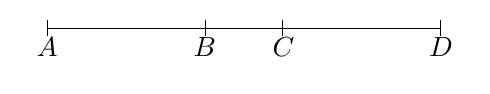
\begin{tikzpicture}
\draw[|-|](0,0)node[below]{$A$}--(5,0)node[below]{$D$};
\draw[|-|](2,0)node[below]{$B$}--(3,0)node[below]{$C$};	
\end{tikzpicture}
	\caption*{第2(a)题}
\end{figurehere}

\item 已知:如图$\angle AOC=\angle BOD$,求证:$\angle AOB=\angle COD$

证明:$\because\quad \angle AOC=\angle BOD$ (\qquad)
	
又$\because\quad \angle BOC=\angle BOC$

$\therefore\quad \angle AOC-\angle BOC=\angle BOD-\angle BOC$ (\qquad )

即 $\angle AOB=\angle COD$。

\item 已知:如图,$C$是$\overline{AB}$的中点,$F$点是$\overline{DE}$的中点,$\overline{AC}=\overline{DF}$,

求证:$\overline{AB}=\overline{DE}$。

证明:$\because\quad \overline{AC}=\overline{DF}$ (\qquad)

$\therefore\quad 2\overline{AC}=2\overline{DF}$ (\qquad)

又$\because\quad C$点,$F$点分别是$\overline{AB}$,$\overline{DE}$的中点(\qquad)

$\therefore\quad 2\overline{AC}=2\overline{AB}$ (\qquad),
$2\overline{DF}=\overline{DE}$(\qquad)。

$\therefore\quad \overline{AB}=\overline{DE}$(\qquad)。

\begin{figurehere}
    \begin{minipage}[b]{0.48\linewidth}
    \centering
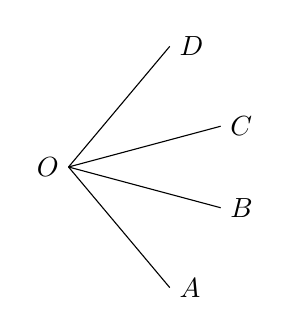
\begin{tikzpicture}[>=latex, scale=1]
       \foreach \x/\xtext in {15/C,-15/B,50/D,-50/A}
{
	\draw(0,0)--(\x:2)node[right]{$\xtext$};
}
\node at (0,0)[left]{$O$};
    \end{tikzpicture}
    \caption*{第2(b)题}
    \end{minipage}
    \begin{minipage}[b]{0.48\linewidth}
    \centering
    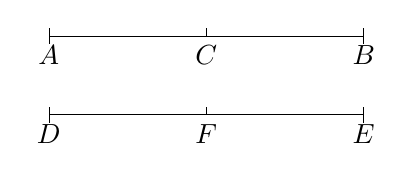
\begin{tikzpicture}[>=latex, scale=1]
      \draw[|-|](0,0)node[below]{$A$}--(4,0)node[below]{$B$};
\draw[|-|](0,-1)node[below]{$D$}--(4,-1)node[below]{$E$};
\node at (2,0)[below]{$C$};
\node at (2,-1)[below]{$F$};
\draw(2,0)--(2,.1);\draw(2,-1)--(2,-1+.1);
    \end{tikzpicture}
    \caption*{第2(c)题}
    \end{minipage}
    \end{figurehere}


\item 已知:如图,$\angle ABC=\angle EFG$,$BD$,$FH$分别是
$\angle ABC$,$\angle FFG$的平分线。

求证:$\angle ABD=\angle HFG$。

证明:$\because\quad BD, FH$分别是$\angle ABC$和$\angle EFG$的平分线(\qquad )

$\therefore\quad \angle ABD=\angle DBC,\quad \angle EFH=\angle HFG$(\qquad)

又$\because\quad \angle ABC=\angle EFG$(\qquad)

$\therefore\quad \angle ABD=\angle HFG$(\qquad)

\begin{figurehere}
    \begin{minipage}[b]{0.48\linewidth}
    \centering
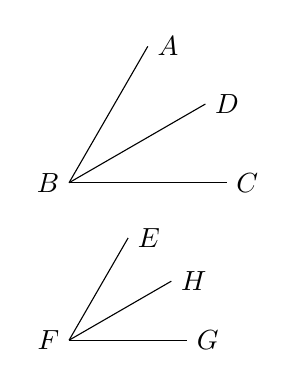
\begin{tikzpicture}[>=latex, scale=1]
      \foreach \x/\xtext in {30/D,60/A,0/C}
{
	\draw(0,0)--(\x:2)node[right]{$\xtext$};
}
\node at (0,0)[left]{$B$}; 

\draw (0,-2)node[left]{$F$}--(1.5,-2)node[right]{$G$};
\draw (0,-2)--(.75*1.732,-2+.75)node[right]{$H$};
\draw (0,-2)--(.75,-2+.75*1.732)node[right]{$E$};       
    \end{tikzpicture}
    \caption*{第2(d)题}
    \end{minipage}
    \begin{minipage}[b]{0.48\linewidth}
    \centering
    \begin{tikzpicture}[>=latex, scale=1]
% \tkzDefPoints{-1/-2/A, 3/-2/B, 1/1/C, -.5/-2.5/D, 2.5/-2.5/E}
% \tkzDrawLines[add =0 and 0](C,D C,E  A,B)
% \tkzInterLL(A,B)(C,D) \tkzGetPoint{F}
% \tkzInterLL(A,B)(C,E) \tkzGetPoint{G}
% \tkzMarkAngles[mark=none, size=.4](A,F,D E,G,B B,F,C C,G,A)
% \tkzLabelAngle[pos=.5](A,F,D){3}
% \tkzLabelAngle[pos=.5](E,G,B){4}
% \tkzLabelAngle[pos=.5](B,F,C){1}
% \tkzLabelAngle[pos=.5](C,G,A){2}
    \end{tikzpicture}
    \caption*{第2(e)题}
    \end{minipage}
    \end{figurehere}

\item 已知:如图,$\angle 1$和$\angle 3$,$\angle 2$和$\angle 4$是对顶角,且$\angle 1=\angle 2$。

求证:$\angle 3=\angle 4$。

证明:$\because\quad \angle 1$和$\angle 3$,$\angle 2$和$\angle 4$是对顶角(\qquad)

$\therefore\quad \angle 1=\angle 3,\; \angle 2=\angle 4$(\qquad)

又$\because\quad \angle 1=\angle 2$(\qquad )

$\therefore\quad \angle 3=\angle 4$(\qquad )

\item 已知:如图,直线$EF$与直线$AB$、$CD$分别相交于
$P$、$Q$两点,且$\angle 1=\angle 2$。

求证:$\angle 2+\angle 3=180^{\circ}$。

证明:$\because\quad AB$是过$P$的直线(\qquad)

$\therefore\quad \angle 1$与$\angle 3$互为补角(\qquad)

即$\angle 1+\angle 3=180^{\circ}$。

又$\because\quad \angle 1=\angle 2$(\qquad)

$\therefore\quad \angle 2+\angle 3=180^{\circ}$(\qquad )。

\item 已知:如图,直线$AO\perp OC$,直线$BO\perp OD$

求证:$\angle 1=\angle 2$。

证明:$\because\quad AO\perp OC$(\qquad )

$\therefore\quad \angle AOC=90^{\circ}$ (\qquad )

即$\angle 1+\angle BOC=90^{\circ}$

$\therefore\quad \angle 1=90^{\circ}-\angle BOC$。

同理:$\angle 2=90^{\circ}-\angle BOC$

$\therefore\quad \angle 1=\angle 2$ (\qquad )

\begin{figurehere}
    \begin{minipage}[b]{0.48\linewidth}
    \centering
\begin{tikzpicture}[>=latex, scale=1.2]
	% \tkzDefPoints{0/0/A, 4/0/B, 0/-1/C, 4/-1/D}
	% \tkzDrawSegments (A,B C,D)
	% \tkzLabelPoints[left](A,C)
	% \tkzLabelPoints[right](B,D)
	% \tkzDefPoints{2/0/P, 1.5/-1/Q}
	% \tkzDrawLines[add =1 and 1](P,Q)
	% \tkzLabelPoints[below](Q)\tkzLabelPoints[above](P)
	% \tkzMarkAngles[mark=none, size=.4](A,P,Q D,Q,P)
	% \tkzLabelAngles[pos=.6](A,P,Q){1} 
	% \tkzLabelAngles[pos=.6](D,Q,P){2}
	% \tkzMarkAngle[mark=none, size=.5](Q,P,B)
	% \tkzLabelAngles[pos=.6](Q,P,B){3}
	% \node at (.8,-2){$F$};
	% \node at (2.8,1){$E$};
    \end{tikzpicture}
    \caption*{第2(f)题}
    \end{minipage}
    \begin{minipage}[b]{0.48\linewidth}
    \centering
    \begin{tikzpicture}[>=latex, scale=1]
% 		\tkzDefPoint(0:0){O}
% 		\tkzDefPoint(0:2.5){D}
% 		\tkzDefPoint(30:2.5){C}
% 		\tkzDefPoint(90:2.5){B}
% 		\tkzDefPoint(120:2.5){A}
% \tkzAutoLabelPoints[center=O](A,B,C,D)
% \tkzDrawSegments(O,A O,B O,C O,D)
% \tkzMarkRightAngles(B,O,D A,O,C)
% \tkzMarkAngles[mark=none, size=.7](D,O,C B,O,A)
% \tkzLabelAngles[pos=.8](D,O,C){2}
% \tkzLabelAngles[pos=.8](B,O,A){1}
% \node at (-.2,-.2){$O$};
    \end{tikzpicture}
    \caption*{第2(g)题}
    \end{minipage}
    \end{figurehere}

\item 已知:如图,$\overline{AB}=\overline{DC}$,$\overline{AC}=\overline{DB}$

求证:$\angle 1=\angle 2$。

证明:在$\triangle ABC$与$\triangle DCB$中

$\because\quad \overline{AB}=\overline{DC},\quad \overline{AC}=\overline{DB}$(\qquad )

又$\because\quad \overline{BC}=\overline{BC}$(\qquad)

$\therefore\quad \triangle ABC\cong \triangle DCB$(\qquad)

$\therefore\quad \angle 1=\angle 2$(\qquad )

\item 已知:如图,$\overline{AC}$与$\overline{BD}$交于$O$点,并且$\overline{OA}=\overline{OC}$,$\overline{OB}=\overline{OD}$。

求证:$\overline{AB}=\overline{CD}$。

证明:在$\triangle AOB$与$\triangle COD$中,

$\because\quad \overline{OA}=\overline{OC},\quad \overline{OB}=\overline{OD}$(\qquad)

又$\because\quad \overline{AC}$与$\overline{BD}$交于$O$点(\qquad)

$\therefore\quad \angle AOB=\angle COD$(\qquad)

$\therefore\quad \triangle AOB\cong\triangle COD$(\qquad)

$\therefore\quad \overline{AB}=\overline{CD}$

\begin{figurehere}
    \begin{minipage}[b]{0.48\linewidth}
    \centering
\begin{tikzpicture}[>=latex, scale=1]
%     \tkzDefPoints{-2/0/B, 2/0/C, -1/3/A, 1/3/D}
% \tkzDrawSegments(A,B A,C B,D B,C D,C)
% \tkzLabelPoints[left](A,B)
% \tkzLabelPoints[right](C,D)
% \tkzMarkAngles[mark=none, size=.4](A,C,B C,B,D)
% \tkzLabelAngles[pos=.6](A,C,B){2}
% \tkzLabelAngles[pos=.6](C,B,D){1}

    \end{tikzpicture}
    \caption*{第2(h)题}
    \end{minipage}
    \begin{minipage}[b]{0.48\linewidth}
    \centering
    \begin{tikzpicture}[>=latex, scale=1]
    \draw(0,0)node[left]{$D$}--(3,0)node[right]{$C$};
\draw(1,3)node[left]{$A$}--(4,3)node[right]{$B$};
\draw(0,0)--(4,3);
\draw(1,3)--(3,0);
\node at (2,1.5)[left]{$O$};
    \end{tikzpicture}
    \caption*{第2(i)题}
    \end{minipage}
    \end{figurehere}

\item 已知:如图,$\angle 1=\angle 2$,$\angle 3=\angle 4$,

求证:$\overline{AC}=\overline{AD}$

证明:$\because\quad \angle 1=\angle 2,\quad \angle 3=\angle 4$(\qquad )

又$\because\quad \overline{AB}=\overline{AB}$(\qquad )

$\therefore\quad\triangle ABC\cong \triangle ABD$(\qquad )

$\therefore\quad \overline{AC}=\overline{AD}$(\qquad )

\begin{figurehere}
    \begin{minipage}[b]{0.48\linewidth}
    \centering
\begin{tikzpicture}[>=latex, scale=1]
	% \tkzDefPoints{0/0/A, 1/1.5/C, 1/-1.5/D, 4/0/B}
	% \tkzDrawSegments(A,C C,B B,D A,D A,B)
	% \tkzLabelPoints[left](A,C,D)
	% \tkzLabelPoint[right](B){$B$}
	% \tkzMarkAngles[mark=none, size=.4](B,A,C A,B,D)
	% \tkzLabelAngles[pos=.6](B,A,C){1}
	% \tkzLabelAngles[pos=.6](A,B,D){4}
	% \tkzMarkAngles[mark=none, size=.5](C,B,A D,A,B)
	% \tkzLabelAngles[pos=.7](C,B,A){3}
	% \tkzLabelAngles[pos=.7](D,A,B){2}
    \end{tikzpicture}
    \caption*{第2(j)题}
    \end{minipage}
    \begin{minipage}[b]{0.48\linewidth}
    \centering
    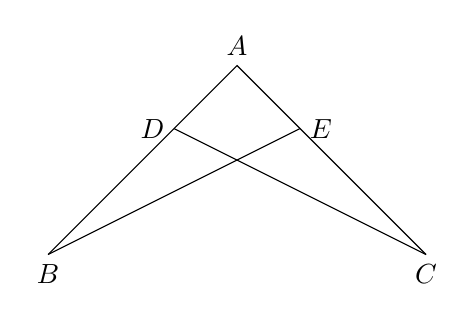
\begin{tikzpicture}[>=latex, scale=.8]
      \draw(-3,0)node[below]{$B$}--(0,3)node[above]{$A$}--(3,0)node[below]{$C$};
\draw(-1,2)node[left]{$D$}--(3,0);
\draw(1,2)node[right]{$E$}--(-3,0);
    \end{tikzpicture}
    \caption*{第3(a)题}
    \end{minipage}
    \end{figurehere}
\end{enumerate}

\item 去掉下列各题中推理的多余步骤。
\begin{enumerate}
	\item 已知;如图,$\overline{AC}=\overline{AB}$,$\overline{AD}=\overline{AE}$。
	
求证:$\angle ADC=\angle AEB$。

证明:在$\triangle ADC$和$\triangle AEB$中,

$\because\quad \overline{AC}=\overline{AB},\quad \overline{AD}=\overline{AE}$(已知)

又$\because\quad \angle A=\angle A$ (公共角)

又$\because\quad \angle B=\angle C$ 

$\therefore\quad \triangle ADC\cong \triangle AEB$(SAS)

$\therefore\quad \angle ADC=\angle AEB$(全等三角形对应角相
等)

\item 已知:如图,$\overline{AB}=\overline{DC},\quad \angle A=\angle D,\quad \angle B=\angle C$

求证:$\overline{BF}=\overline{CE}$。

证明:在$\triangle ABE$与$\triangle DCF$中,

$\because\quad \overline{AB}=\overline{DC},\quad \angle A=\angle D,\quad \angle B=\angle C$(已知)

又$\because\quad \angle 1=\angle 2$

$\therefore\quad \triangle ABE\cong \triangle DCF$(ASA)

$\therefore\quad \overline{BE}=\overline{CF}$(全等三角形的对应边相等)

又$\because\quad \overline{EF}=\overline{EF}$

$\therefore\quad \overline{BF}=\overline{CE}$(等量减等量差相等)
\end{enumerate}

\begin{figurehere}
    \begin{minipage}[b]{0.48\linewidth}
    \centering
\begin{tikzpicture}[>=latex, scale=1]
% \tkzDefPoints{0/0/C, 2/0/D, 2/3/F, 1/1.5/E, 1/4.5/A, 3/4.5/B}
% \tkzDrawSegments(B,C F,D A,E A,B C,D)
% \tkzLabelPoints[left](A,C,E)
% \tkzLabelPoints[right](B,F,D)
% \tkzMarkAngles[mark=none, size=.5](C,F,D B,E,A)
% \tkzLabelAngles[pos=.7](C,F,D){1}
% \tkzLabelAngles[pos=.7](B,E,A){2}
    \end{tikzpicture}
    \caption*{第3(b)题}
    \end{minipage}
    \begin{minipage}[b]{0.48\linewidth}
    \centering
    \begin{tikzpicture}[>=latex, scale=1]
% \tkzDefPoints{-2.5/0/D, 2.5/0/B, -1/2.5/A, 1/2.5/C}
% \tkzDrawSegments(A,B A,D B,C C,D)
% \tkzLabelPoints[left](A,D)
% \tkzLabelPoints[right](C,B)
% \node at (0,1.5){$O$};
    \end{tikzpicture}
    \caption*{第4(a)题}
    \end{minipage}
    \end{figurehere}

\item 补上下列各题推理中所缺少的必要步骤。
\begin{enumerate}
	\item 已知;如图,$\overline{AB}$,$\overline{CD}$相交于$O$点,并且$\overline{AO}=\overline{OC}$,$\overline{OD}=\overline{OB}$。

求证:$\angle D=\angle B$,$\overline{AD}=\overline{BC}$。

证明:在$\triangle AOD$和$\triangle COB$中,

$\because\quad \overline{AO}=\overline{OC}$(已知)

又$\because\quad \overline{AB}$,$\overline{CD}$相交于$O$点(已知)

$\therefore\quad \angle AOD=\angle COB$(对顶角相等)

$\therefore\quad \triangle AOD\cong \triangle COB$(SAS)

$\therefore\quad \angle D=\angle B$(全等三角形的对应角相等),
$\overline{AD}=\overline{BC}$(全等三角形的对应边相等)。

\item 已知:如图,$\overline{AD}=\overline{BC}$,$\overline{AB}=\overline{CD}$。

求证:$\angle B=\angle D$。

证明:在$\triangle ABC$与$\triangle CDA$中

$\because\quad \overline{AD}=\overline{BC},\quad \overline{AB}=\overline{CD}$(已知)

$\therefore\quad \triangle ABC\triangle CDA$(SSS)

$\therefore\quad \angle B=\angle D$(全等三角形的对应角相等)。


\end{enumerate}

\begin{figurehere}
    \begin{minipage}[b]{0.48\linewidth}
    \centering
\begin{tikzpicture}[>=latex, scale=1]
	% \tkzDefPoints{0/0/B, 3/0/C, 1/2/A, 4/2/D}
	% \tkzDrawSegments(A,B A,C A,D B,C D,C)
	% \tkzLabelPoints[left](A,B)
	% \tkzLabelPoints[right](C,D)
    \end{tikzpicture}
    \caption*{第4(b)题}
    \end{minipage}
    \begin{minipage}[b]{0.48\linewidth}
    \centering
    \begin{tikzpicture}[>=latex, scale=1]
% \tkzDefPoint(0:3){A}
% \tkzDefPoint(60:3){C}
% \tkzDefPoint(30:3){B}
% \tkzDefPoint(20:3){A1}
% \tkzDefPoint(50:3){A2}
% \tkzDefPoint(0,0){O}
% \tkzDrawSegments(O,A O,B O,C O,A1 O,A2)
% \tkzLabelPoints[right](A,B,C)
% \node at (-.2,-.2){$O$};

% \draw(1,0) arc (0:20:1);
% \draw(20:1.5) arc (20:30:1.5);
% \draw(30:1) arc (30:50:1);
% \draw(50:1.5) arc (50:60:1.5);
% \node at (10:1.2){1};
% \node at (25:1.8){2};
% \node at (40:1.2){3};
% \node at (55:1.8){4};
    \end{tikzpicture}
    \caption*{第5题}
    \end{minipage}
    \end{figurehere}

\item 已知:如图,$OB$是$\angle AOC$的平分线,并且$\angle 1=\angle 4$,

求证:$\angle 2=\angle 3$。
\item 已知:如图,$\angle 2$与$\angle 3$是对顶角,且$\angle 1=\angle 3$,

求证:$\angle 1=\angle 2$。
\item 已知:如图,$\overline{AB}=\overline{AC}$,$D$是$\overline{BC}$的中点,

求证:$\triangle ABD\cong \triangle ACD$。
\begin{figurehere}
    \begin{minipage}[b]{0.48\linewidth}
    \centering
\begin{tikzpicture}[>=latex, scale=1]
	% \tkzDefPoints{0/0/A, 4/0/B, 0/-1/C, 4/-1/D}
	% \tkzDrawSegments (A,B C,D)
	% \tkzDefPoints{2/0/P, 1.5/-1/Q, 2.5/1/E}
	% \tkzDrawLines[add =1 and 1](P,Q)
	% \tkzMarkAngles[mark=none, size=.4](A,P,Q D,Q,P B,P,E)
	% \tkzLabelAngles[pos=.6](A,P,Q){2} 
	% \tkzLabelAngles[pos=.6](D,Q,P){1}
	% \tkzLabelAngles[pos=.6](B,P,E){3}

    \end{tikzpicture}
    \caption*{第6题}
    \end{minipage}
    \begin{minipage}[b]{0.48\linewidth}
    \centering
    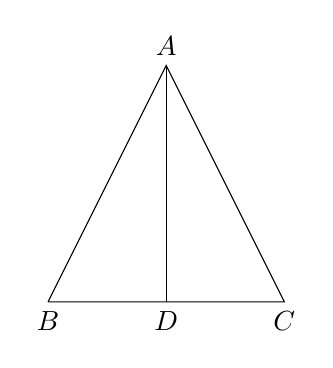
\begin{tikzpicture}[>=latex, scale=1]
		\draw(-1.5,0)node[below]{$B$}--(0,0)node[below]{$D$}--(1.5,0)node[below]{$C$}--(0,3)--(-1.5,0);
\draw(0,3)node[above]{$A$}--(0,0);
    \end{tikzpicture}
    \caption*{第7题}
    \end{minipage}
    \end{figurehere}

\item 已知:如图,$\overline{AB}\perp \overline{BD}$,$\overline{CD}\perp \overline{BD}$,$O$ 是 $\overline{BD}$ 的中点,
$\overline{AC}$与$\overline{BD}$交于$O$。

求证:$\triangle ABO\cong \triangle CDO$。
\item 已知;如图,$BD$平分$\angle ABC$,并且$\overline{AB}=\overline{BC}$,

求证:$\triangle ABD\cong \triangle CBD$。
\begin{figurehere}
    \begin{minipage}[b]{0.48\linewidth}
    \centering
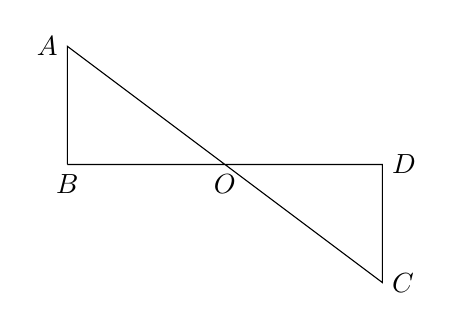
\begin{tikzpicture}[>=latex, scale=1]
\draw(0,0)node[below]{$B$}--(4,0)node[right]{$D$}--(4,-1.5)node[right]{$C$}--(2,0)node[below]{$O$}--(0,1.5)node[left]{$A$}--(0,0)  ;
    \end{tikzpicture}
    \caption*{第8题}
    \end{minipage}
    \begin{minipage}[b]{0.48\linewidth}
    \centering
    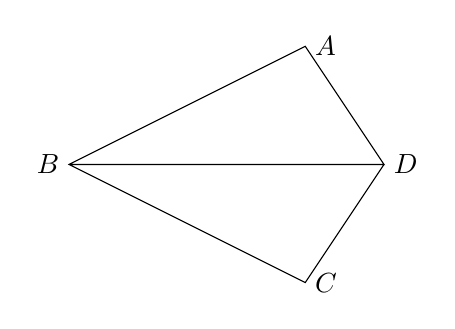
\begin{tikzpicture}[>=latex, scale=1]
      \draw(0,0)node[left]{$B$}--(4,0)node[right]{$D$}--(3,1.5)node[right]{$A$}--(0,0)--(3,-1.5)node[right]{$C$}--(4,0);
    \end{tikzpicture}
    \caption*{第9题}
    \end{minipage}
    \end{figurehere}
\end{question}
\end{Exercise}


\begin{Exercise}[复习题]
\begin{question}
	\item 试举出五个集合的例子,并用列举法或描述法表示出来。
	\item 写出下列集合的所有元素。
\begin{enumerate}
	\item $A=\{\text{绝对值小于10的2的倍数}\}$
	\item $B=\{\text{绝对值小于40的5的倍数}\}$
	\item $C=\{\text{绝对值小于20的3的倍数}\}$
\end{enumerate}

\item 用特征性质描述法表示下列集合:
\begin{enumerate}
	\item 一切偶数的集合。
	\item 一切奇数的集合。
	\item 大于等于0, 而小于等于1的实数集合。
\end{enumerate}

\item 下列命题是否正确?
\begin{enumerate}
	\item 一个正方形是正方形集合的一个元素。
	\item 飞机是飞机场集合的一个元素。
	\item 某校一成员是这校全体学生构成的集合的一个元素。
\end{enumerate}

\item 指出下列集合中的元素:
\begin{enumerate}
	\item $A=\{x|x<15\text{ 且 $x$ 是质数}\}$
	\item $B=\{x|x^2=0\text{ 且 $x$ 是实数}\}$
\end{enumerate}

\item 设$A=\{1,2,3,4\}$,$B=\{ 2,4,6,8\}$,$C=\{3,4,5,6\}$,求:
\begin{tasks}(4)
	\task $A\cup B$
	\task $A\cup C$
	\task $B\cup C$
	\task $(A\cup B)\cup C$
	\task $A\cup (B\cup C)$
	\task $A\cap B$
	\task $A\cap C$
	\task $B\cap C$
	\task $(A\cap B)\cap C$
	\task $A\cap (B\cap C)$
\end{tasks}	


\item 如图,$A$、$B$、$C$ 三个集合相交成非空集,用阴影分别把下列各集合所表示的区域划出来。
\begin{tasks}(4)
	\task $A\cap B$
	\task $A\cup B$
	\task $A\cap C$
	\task $A\cup C$
	\task $B\cap C$
	\task $B\cup C$
	\task $A\cap (B\cap C)$
	\task $(A\cap B)\cap C$
	\task $A\cup (B\cup C)$
	\task $(A\cup B)\cup C$
\end{tasks}	

\begin{figurehere}
    \begin{minipage}[b]{0.48\linewidth}
    \centering
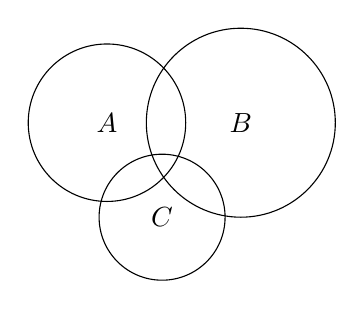
\begin{tikzpicture}[>=latex, scale=1]
       \draw (0,0)node{$A$} circle (1);
	\draw (1.7,0) node{$B$} circle (1.2);
	\draw (.7,-1.2) node{$C$} circle (.8);
    \end{tikzpicture}
	\caption*{第7题}
    \end{minipage}
    \begin{minipage}[b]{0.48\linewidth}
    \centering
    \begin{tikzpicture}[>=latex, scale=1]
% \tkzDefPoints{0/0/B, -1/2/A, 1/2/C, 0/3.5/E, 0/2.75/D}
% \tkzDrawLines[add=0 and .5](B,A B,C B,D)
% \tkzLabelPoints[left](A,B)
% \tkzLabelPoints[right](C,D)
% \draw(A)--(D)--(C);
% \tkzMarkAngles[mark=none, size=.45](E,D,A E,B,A)
% \tkzMarkAngles[mark=none, size=.5](C,D,E C,B,E)
% \tkzLabelAngle[pos=.6](E,D,A){1}
% \tkzLabelAngle[pos=.7](E,B,A){3}
% \tkzLabelAngle[pos=.6](C,D,E){2}
% \tkzLabelAngle[pos=.7](C,B,E){4}
% \node at (0,3.8)[right]{$E$};
    \end{tikzpicture}
	\caption*{第11题}
    \end{minipage}
    \end{figurehere}

\item 设基集${\rm I}=\{1,2,3,4,5,6,7,8,9,10\}$,
$A=\{6,8,9\}$,$B=\{ 1, 3, 7,8,9\}$,
$C=\{2,6,8,9\}$。求:
\begin{tasks}(4)
	\task $A^c$
	\task $B^c$
	\task $C^c$
	\task $(A\cap B)^c$
	\task $(A^c)\cap (B^c)$
	\task $(A\cup B)^c$
	\task $(A^c)\cup (B^c)$
\end{tasks}	

\item 写出列各命题中的“已知”部分和“求证”部分。
\begin{enumerate}
	\item 三角形三个角的和等于$180^{\circ}$。
	\item 角平分线上任一点到角的两边距离相等。
\end{enumerate}

\item 在下列各题的(\qquad)中,适当地填上“必要不充分”,
“充分不必要”,“充分必要”等词。
\begin{enumerate}
	\item $a=0$是$ab=0$的(\qquad)条件。
	\item 两个角相等是两个角为对顶角的(\qquad)条件。
	\item 形状和大小完全相同的两个图形是全等形的(\qquad)
	条件。
	\item $a^2=b^2$是$a=b$的(\qquad)条件。
	\item 多项式$P(x)$被$x-\alpha$整除是$P(\alpha)=0$的(\qquad)
	条件。
	\item $a\ne b$ 是$a^2+b^2>2ab$的(\qquad)条件。
\end{enumerate}

\item 已知:如图,$\angle 1=\angle 2$,$\angle 3=\angle 4$,$BE$是直线。

求证:$\overline{AD}=\overline{CD}$。

\item 已知:如图,$\overline{AB}=\overline{DE}$,$\overline{AC}=\overline{DF}$,$\overline{BC}=\overline{EF}$。

求证:$\angle 1=\angle 2$,$AC\parallel DF$。
\item 已知:如图,$\angle 1=\angle 2$,$\overline{AD}=\overline{BC}$。

求证:$\angle B=\angle D$,$\overline{AB}=\overline{CD}$。

\begin{figurehere}
  \begin{minipage}[b]{0.48\linewidth}
    \centering
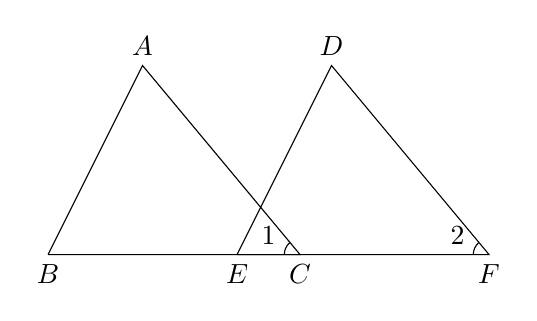
\begin{tikzpicture}[>=latex, scale=.8]
\draw (0,0)node[below]{$B$}--(4,0)node[below]{$C$}--(1.5,3)node[above]{$A$}--(0,0);
\draw (3,0)node[below]{$E$}--(7,0)node[below]{$F$}--(4.5,3)node[above]{$D$}--(3,0);
\foreach \x/\xtext in {4/1,7/2}
{
	\draw (\x-.25,0) arc (180:130:.25);
	\draw(\x-.5,0)node[above]{$\xtext$};
}
    \end{tikzpicture}
	\caption*{第12题}
    \end{minipage}
    \begin{minipage}[b]{0.48\linewidth}
    \centering
    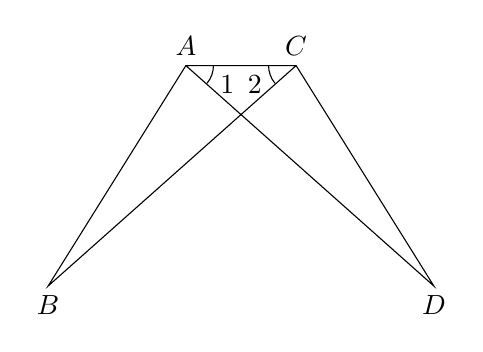
\begin{tikzpicture}[>=latex, scale=.7]
    \draw(1,0)--(-3.5,-4)node[below]{$B$}--(-1,0)node[above]{$A$}--(1,0)node[above]{$C$}--(3.5,-4)node[below]{$D$}--(-1,0);
	\draw (1-.5,0) arc (180:220:.5);
	\draw (-1+.5,0) arc (0:-40:.5);
	\draw(1-.75,0)node[below]{2};\draw(-1+.75,0)node[below]{1};
    \end{tikzpicture}
	\caption*{第13题}
    \end{minipage}
  \end{figurehere}
	\item 证明:同角的补角相等。
	\item 证明:等角的余角相等。
	\item 证明:等角的补角相等。
\end{question}
\end{Exercise}
\chapter{直线形}

在\cref{chp:experiment_geometry}里,我们从日常生活所熟悉的位置、通路、方向、叠合出发,讨论了空间的几个重要的基本概念:点、直线、平行、全等、相似,并通过观察、实验,分析归纳出了空间的一些性质。在\cref{chp:logic}中,我们把其中的某些性质作为基本性质和定理。在本章中,我们将以这些基本性质和定理为基础,运用\cref{chp:logic}所介绍的演绎法去推演空间的其它性质。演绎法不但是研究几何学的基本有效方法,在其它任何科学的研究中也都是十分重要的方法。概括地说,对于科学研究,实验归纳和论证推演是互相配合使用的两种基本科学方法,它们是探索科学规律的两条腿。从这一章起,我们对空间性质的探讨,主要用演绎法来进行。
\section{三角形}
\subsection{全等三角形}

\begin{Definition}
平面上顺次首尾端点相接且不在同一条直线上的线段组成的封闭图形叫做\Concept{多边形}。这些线段叫做\Concept{多边形的边},它们的端点叫做\Concept{多边形的顶点},每相邻两边的夹角叫做多边形的\Concept{内角}。
\end{Definition}

三角形是多边形中最简单的图形。有四条边的多边形叫做四边形,有五条边的多边形叫五边形……等等。表示一个多边形可用顶点的名称,沿周界顺次列出,如\cref{fig:3-1} 中的 $\triangle ABC$,四边形 $ABCD$ ……等等。

如果多边形都在每边所在直线的同旁,我们称这种多边形为\Concept{凸多边形}(\cref{fig:3-1} 中的三个图形都是凸多边形,\cref{fig:3-2} 中的图形则不是)。以后我们说多边形时,都指的是凸多边形。
\begin{figure}
    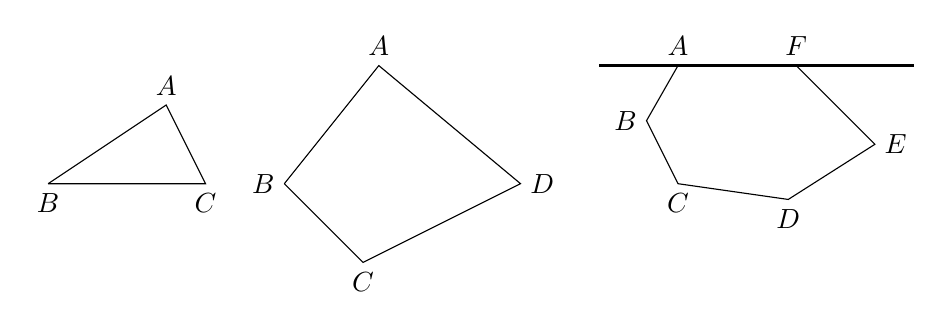
\begin{tikzpicture}
\begin{scope}
\draw(0,0)node[below]{$B$}--(2,0)node[below]{$C$}--(1.5,1)node[above]{$A$}--(0,0);
\end{scope}
\begin{scope}[xshift=3cm]
\draw (0,0)node[left]{$B$}--(1,-1)node[below]{$C$}--(3,0)node[right]{$D$}--(1.2,1.5)node[above]{$A$}--(0,0);
\end{scope}
\begin{scope}[xshift=8cm, yshift=1.5cm]
\draw (0,0)node[above]{$A$}--(1.5,0)node[above]{$F$}--(2.5,-1)node[right]{$E$}--(1.4,-1.7)node[below]{$D$}--(0,-1.5)node[below]{$C$}--(-.4,-.7)node[left]{$B$}--(0,0);
\draw[thick](-1,0)--(3,0);
\end{scope}        
    \end{tikzpicture}
    \caption{}\label{fig:3-1}
\end{figure}

\begin{figure}
    \centering
\begin{tikzpicture}
\draw[dashed](-2,0)--(2,0);
\draw (-.5,0)--(0.2,0)--(.3,-1)--(.7,1.8)--(-.5,0);
\end{tikzpicture}
    \caption{}\label{fig:3-2}
\end{figure}

\begin{Definition}{定义}
两个能够完全叠合的三角形叫做\Concept{全等三角形}。两个全等三角形完全叠合时,互相叠合的顶点叫做\Concept{对应点},互相叠合的边叫做\Concept{对应边},互相叠合的角叫做\Concept{对应角}。因此,\emph{全等三角形的对应边相等,对应角相等}。
\end{Definition}
 
怎样判定两个三角形全等呢?
\begin{enumerate}
  \item 有两边和它们的夹角对应相等的两个三角形全等。(SAS)
  \item 有两角和它们的夹边对应相等的两个三角形全等。(ASA)
  \item 有三边对应相等的两个三角形全等。(SSS)
\end{enumerate}

利用三角形的全等,是判断两条线段或两个角相等的一种基本方法。

\begin{example}
在\cref{fig:3-3} 中,已知 $\overline{AB}=\overline{AC}$,$\angle B=\angle C$,求证:$\overline{BD}=\overline{CE}$。
\end{example}

\begin{analyze}
要证 $\overline{BD}=\overline{CE}$,从图上看 $\overline{BD}$,$\overline{CE}$ 分别是 $\triangle ABD$ 和 $\triangle ACE$ 的边,因此只要证明 $\triangle ACE \cong \triangle ABD$ 就行了,由已知条件 $\overline{AC}=\overline{AB}$,$\angle B=\angle C$ 而 $\angle A$ 是公共角,所以 $\triangle ABD$ 与 $\triangle ACE$ 全等是很显然的。
\end{analyze}

\begin{proof}
在 $\triangle ABD$ 与 $\triangle ACE$ 中,

$\because\quad \overline{AB}=\overline{AC},\quad \angle B=\angle C$(已知)。

而 $\angle A=\angle A$(公共角),

$\therefore\quad \triangle ABD\cong \triangle ACE$ (ASA)。

$\therefore\quad \overline{BD}=\overline{CE}$ (全等三角形的对应边相等)。
\end{proof}    

\begin{figure}
  \begin{minipage}[b]{0.48\linewidth}
    \centering
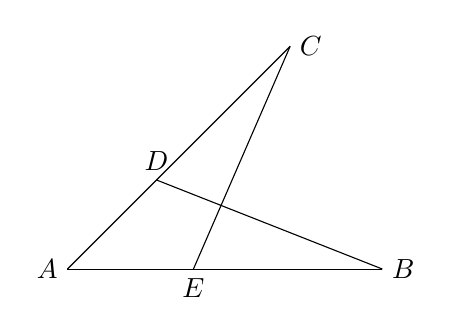
\begin{tikzpicture}[>=latex, scale=.8]
       \draw (0,0)node[left]{$A$}--(5,0)node[right]{$B$};
\draw (0,0)--(45:5)node[right]{$C$};
\draw (2,0)node[below]{$E$}--(45:5);
\draw (45:2)node[above]{$D$}--(5,0);
    \end{tikzpicture}
    \caption{}
  \end{minipage}
  \begin{minipage}[b]{0.48\linewidth}
    \centering
    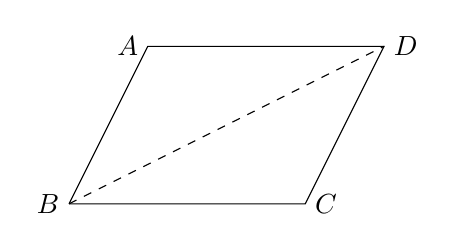
\begin{tikzpicture}[>=latex, scale=1]
        \draw (0,0)node[left]{$B$}--(3,0)node[right]{$C$}--(4,2)node[right]{$D$}--(1,2)node[left]{$A$}--(0,0);
        \draw[dashed](0,0)--(4,2);   
    \end{tikzpicture}
    \caption{}\label{fig:3-3}
  \end{minipage}
\end{figure}


\begin{example}
已知:在四边形 $ABCD$ 中,$\overline{AD}=\overline{BC}$,$\overline{AB}=\overline{CD}$(图3.4)。

求证:$\angle A=\angle C$。
\end{example}

\begin{analyze}
要证明$\angle A=\angle C$,需要把四边形 $ABCD$ 分成两个三角形,为此,连结 $B$、$D$。这叫做添\Concept{辅助线}。这样只需证 $\triangle ABD\cong \triangle CDB$ 就行了。
\end{analyze}

\begin{proof}
连结 $B$、$D$,在 $\triangle ABD$ 与 $\triangle CDB$ 中,

$\because\quad \overline{AD}=\overline{BC},\quad \overline{AB}=\overline{CD}$ (已知)

又 $\because\quad \overline{BD}=\overline{BD}$ (公共边)

$\therefore\quad \triangle ABD\cong \triangle CDB$ (SSS)

$\therefore\quad \angle A=\angle C$(全等三角形的对应角相等)。
\end{proof}    

\begin{example}
在图3.5中,已知:$\overline{AB}=\overline{CD}$,$\angle B=\angle CDF$,$\overline{BD}=\overline{EF}$。

求证:$\overline{AE}=\overline{CF}$。
\end{example}

\begin{analyze}
    要证$\overline{AE}=\overline{CF}$,只需证$\triangle ABE\cong \triangle CDF$。由已
知,$\overline{AB}=\overline{CD}$,$\angle B=\angle CDF$,$\overline{BD}=\overline{EF}$,虽然不能马上说
$\triangle ABE$和$\triangle CDF$全等,但只要注意到$\overline{BD}+\overline{DE}=\overline{DE}+\overline{EF}$,
即$\overline{EB}=\overline{DF}$就行了。
\end{analyze}

\begin{proof}
    在图3-5中,$\because\quad \overline{BD}=\overline{EF}$ 已知

$\therefore\quad \overline{BD}+\overline{DE}=\overline{DE}+\overline{EF}$ (等量加等量和相等)。即:
\[\overline{BE}=\overline{DF}\]
又$\because\quad \overline{AB}=\overline{CD},\; \angle B =\angle CDF$ 已知

$\therefore\quad \triangle ABE\cong \triangle CDF$ (SAS).

$\therefore\quad \overline{AE}=\overline{CF}$ (全等三角形的对应边相等)。
\end{proof}

\begin{figure}
    \begin{minipage}[t]{0.48\linewidth}
    \centering
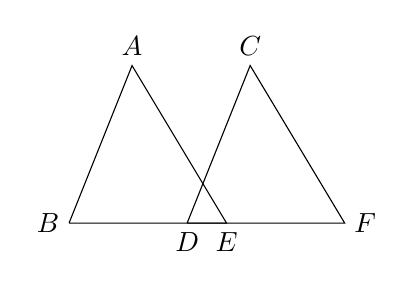
\begin{tikzpicture}[>=latex, scale=1]
       \draw(0,0)node[left]{$B$}--(2,0)node[below]{$E$}--(.8,2)node[above]{$A$}--(0,0);
\draw(1.5,0)node[below]{$D$}--(3.5,0)node[right]{$F$}--(2.3,2)node[above]{$C$}--(1.5,0);
    \end{tikzpicture}
    \caption{ }
    \end{minipage}
    \begin{minipage}[t]{0.48\linewidth}
    \centering
    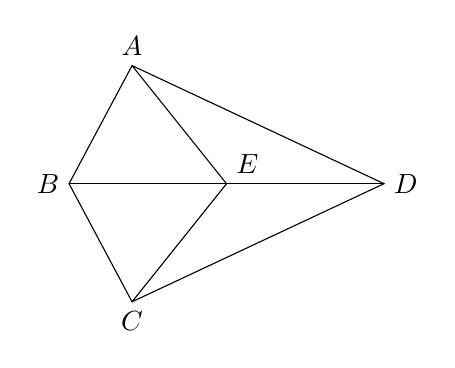
\begin{tikzpicture}[>=latex, xscale=.8]
      \draw(0,0)node[left]{$B$}--(5,0)node[right]{$D$};
      \draw(1,1.5)node[above]{$A$}--(2.5,0)node[above right]{$E$}--(1,-1.5)node[below]{$C$}--(0,0)--(1,1.5)--(5,0)--(1,-1.5);
    \end{tikzpicture}
    \caption{ }
    \end{minipage}
    \end{figure}

\begin{example}
    在图3.6中,已知:$\overline{AB}=\overline{BC}$,$\overline{AD}=\overline{CD}$,$E$点在$BD$上。

求证:$\overline{AE}=\overline{CE}$。
\end{example}

\begin{analyze}
    要证$\overline{AE}=\overline{CE}$,只需证明$\triangle ABE\cong \triangle CBE$,或者证明$\triangle ADE\cong \triangle CDE$,假定我们证明$\triangle ABE\cong \triangle CBE$,
    已知$\overline{AB}=\overline{BC}$,$\overline{BE}=\overline{BE}$,因此只需证明$\angle ABD=\angle CBD$;
    要证$\angle ABD=\angle CBD$,只需证明$\triangle ABD\cong\triangle CBD$。
\end{analyze}

\begin{proof}
    在$\triangle ABD$与$\triangle CBD$中,

    $\because\quad \overline{AB}=\overline{CB},\quad \overline{AD}=\overline{CD}$ (已知)   $\overline{BD}=\overline{BD}$(公共边)

    $\therefore\quad \triangle ABD\cong \triangle CBD$ (SSS).

    $\therefore\quad \angle ABD=\angle CBD$ (全等三角形的对应角相等)

$\because\quad     \overline{AB}=\overline{BC}$ (已知) 
    $\overline{BE}=\overline{BE}$ (公共边)

$\therefore\quad \triangle ABE\cong \triangle CBE$ (SAS).

$\therefore\quad \overline{AE}=\overline{CE}$ (全等三角形的对应边相等)。
\end{proof}

    利用三角形全等,来证明两条线段或两个角相等,关键
    在于找出能够全等的三角形,并且使要证明的线段和角恰好
    成为它们的对应边和对应角。为了找出全等的三角形,必要
    时需要添加辅助线。  

\begin{Practice}
\begin{question}
  \item 已知:在四边形 $ABCD$ 中,$AC$ 平分 $\angle BAD$,$\overline{AB}=\overline{AD}$。求证:$\angle ACB=\angle ACD$。
  \item 已知:如图,$\overline{AC}$、$\overline{BD}$ 交于 $O$ 点,且 $\overline{AO}=\overline{OC}$、$\overline{BO}=\overline{OD}$。求证:$\overline{AB}=\overline{CD}$。


\item 已知:如图,$\angle 1=\angle 4$,$\angle 2=\angle 3$。
求证:$\overline{AB}=\overline{CD}$。
\item 已知:如图,$\angle 1=\angle 2$,$\angle 3=\angle 4$,$\overline{AB}=\overline{AD}$。

求证:$\overline{AE}=\overline{AC}$,$\angle E=\angle C$。

\item 已知:如图,$\angle 1=\angle 2$,$\angle 3=\angle 4$,
求证:$\overline{AC}=\overline{BD}$。
\item 已知:如图,在四边形$ABCD$中,$\overline{AB}=\overline{BC}$,$\overline{AD}=\overline{CD}$。

求证:$\angle A=\angle C$。
\item 已知:如图,$\overline{AD}=\overline{BE}$,$\overline{AE}=\overline{BD}$,AC、BC是直线。

求证:$\angle CDB=\angle CEA$。
\item 已知:如图,$\overline{AB}=\overline{CD}$,E、F分别是$\overline{AB}$、$\overline{CD}$的中点,
并且$\overline{BF}=\overline{CE}$。

求证:$\angle EBC=\angle FCB$,$\angle FBC=\angle ECB$。

\item 已知:如图,在四边形$ABCD$中,$\overline{AB}=\overline{CD}$,$\overline{AD}=\overline{BC}$,$\overline{EF}$过$\overline{BD}$的中点$O$。

求证:$\overline{OE}=\overline{OF}$。
\end{question}
\end{Practice}

\begin{figure}
    \begin{minipage}[t]{0.48\linewidth}
    \centering
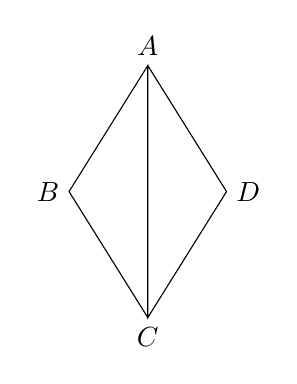
\begin{tikzpicture}[>=latex, yscale=.8]
       \draw(0,2)node[above]{$A$}--(1,0)node[right]{$D$}--(0,-2)node[below]{$C$}--(0,2)--(-1,0)node[left]{$B$}--(0,-2);
    \end{tikzpicture}
    \caption*{第1题}
    \end{minipage}
    \begin{minipage}[t]{0.48\linewidth}
    \centering
    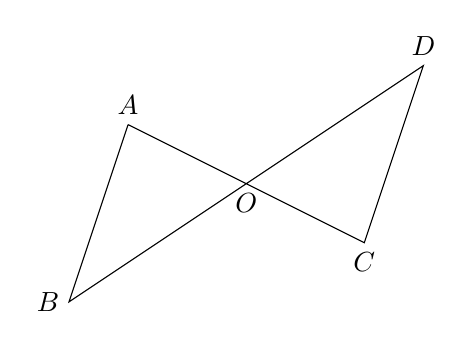
\begin{tikzpicture}[>=latex, scale=1.5]
      \draw(-1,.5)node[above]{$A$}--(1,-.5)node[below]{$C$}--(1.5,1)node[above]{$D$}--(-1.5,-1)node[left]{$B$}--(-1,.5);
      \node at (0,0)[below]{$O$};
    \end{tikzpicture}
    \caption*{第2题}
    \end{minipage}
    \end{figure}

\begin{figure}
    \begin{minipage}[t]{0.48\linewidth}
    \centering
\begin{tikzpicture}[>=latex, scale=1.3]
% \tkzDefPoints{1/2/A, 0/0/B, 3/0/C, 4/2/D}
% \tkzDrawPolygon(A,B,C)
% \tkzDrawPolygon(A,D,C)
% \tkzMarkAngle[mark=none, size=.35](B,A,C)  
% \tkzLabelAngle[pos=.5](B,A,C) {2}
% \tkzMarkAngle[mark=none, size=.5](C,A,D)  
% \tkzLabelAngle[pos=.7](C,A,D) {1}
%  \tkzLabelAngle[pos=.75](A,C,B) {4}
% \tkzMarkAngle[mark=none, size=.5](D,C,A)  
% \tkzLabelAngle[pos=.25](D,C,A) {3}
% \tkzMarkAngle[mark=none, size=.6](A,C,B) 
% \tkzLabelPoints[left](A,B)
% \tkzLabelPoints[right](C,D)
    \end{tikzpicture}
    \caption*{第3题}
    \end{minipage}
    \begin{minipage}[t]{0.48\linewidth}
    \centering
    \begin{tikzpicture}[>=latex, scale=1.3]
    % \tkzDefPoint(0,0){A}
    % \tkzDefPoint(-90:2){B}
    % \tkzDefPoint(-60:2){D}
    % \tkzDefPoint(0:2.75){E}
    % \tkzDefPoint(-30:2.75){C}
    % \tkzLabelPoints[left](A,B)
    % \tkzDrawPolygon(A,B,D)
    % \tkzDrawLines[add=0 and 1.38](B,D) %\tkzGetPoint{C}
    % \draw (D)--(E)--(A)--(C);
    % \tkzLabelPoints[right](C,E)
    % \tkzLabelPoints[below](D)
    % \tkzMarkAngles[mark=none, size=.44](C,A,E B,A,D C,B,A E,D,A)  
    % \tkzLabelAngle[pos=.65](C,A,E) {2}
    % \tkzLabelAngle[pos=.65](B,A,D) {1}
    % \tkzLabelAngle[pos=.6](C,B,A) {3}
    % \tkzLabelAngle[pos=.6](E,D,A) {4}
    \end{tikzpicture}
    \caption*{第4题}
    \end{minipage}
    \end{figure}



\begin{figure}
    \begin{minipage}[t]{0.48\linewidth}
    \centering
\begin{tikzpicture}[>=latex, scale=1]
% \tkzDefPoints{-1/2/A, 1/2/D, -2/-1/B, 2/-1/C}
% \tkzDrawPolygon(A,C,D) \tkzDrawPolygon(A,B,D)
% \tkzLabelPoints[left](A,B)
% \tkzLabelPoints[right](C,D)
% \tkzMarkAngles[mark=none, size=.6](C,A,D A,D,B) 
% \tkzMarkAngles[mark=none, size=.5](B,A,C B,D,C) 
% \tkzLabelAngle[pos=.7](C,A,D) {1}
% \tkzLabelAngle[pos=.7](A,D,B) {2}
% \tkzLabelAngle[pos=.65](B,A,C) {3}
% \tkzLabelAngle[pos=.65](B,D,C) {4}
    \end{tikzpicture}
    \caption*{第5题}
    \end{minipage}
    \begin{minipage}[t]{0.48\linewidth}
    \centering
    \begin{tikzpicture}[>=latex, scale=1.3]
        % \tkzDefPoints{-1/0/B, 2/0/D, 1/1/A, 1/-1/C, 0/0/O} 
        % \tkzDrawPolygon(A,B,C,D)
        % \tkzAutoLabelPoints[center=O](A,B,C,D)
    \end{tikzpicture}
    \caption*{第6题}
    \end{minipage}
    \end{figure}




\begin{figure}
    \begin{minipage}[t]{0.48\linewidth}
    \centering
\begin{tikzpicture}[>=latex, scale=1]
    % \tkzDefPoints{-1.5/0/A, 1.5/0/B, 0/3/C, 0/1.5/O}  
    % \tkzDefMidPoint(A,C)\tkzGetPoint{D}
    % \tkzDefMidPoint(B,C)\tkzGetPoint{E}    
    % \tkzDrawPolygon(A,B,C)
    % \draw(B)--(D)node[left]{$D$};
    % \draw (A)--(E)node[right]{$E$};
    % \tkzAutoLabelPoints[center=O](A,B,C)
    \end{tikzpicture}
    \caption*{第7题}
    \end{minipage}
    \begin{minipage}[t]{0.48\linewidth}
    \centering
    \begin{tikzpicture}[>=latex, scale=.8]
        % \tkzDefPoints{-2.5/0/B, 2.5/0/C, -1.5/3/A, 1.5/3/D,  0/1.5/O}  
        % \tkzDefMidPoint(A,B)\tkzGetPoint{E}
        % \tkzDefMidPoint(D,C)\tkzGetPoint{F}    
        % \tkzDrawPolygon(A,B,C,D)
        % \draw(B)--(F)node[right]{$F$};
        % \draw (C)--(E)node[left]{$E$};
        % \tkzAutoLabelPoints[center=O](A,B,C,D)
    \end{tikzpicture}
    \caption*{第8题}
    \end{minipage}
    \end{figure}


\begin{figure}
    \begin{minipage}[t]{0.48\linewidth}
    \centering
\begin{tikzpicture}[>=latex, scale=.8]
    % \tkzDefPoints{-2.5/0/B, 2.5/0/C, -1.5/3/A, 3.5/3/D}  
    % \tkzDefMidPoint(D,B)\tkzGetPoint{O}
    % \tkzDrawPolygon(A,B,C,D)
    % \draw (0,3)node[above]{$E$}--(1,0)node[below]{$F$};
    % \tkzAutoLabelPoints[center=O](A,B,C,D)
    % \draw(B)--(D);
    % \node at (O)[right]{$O$};

    \end{tikzpicture}
    \caption*{第9题}
    \end{minipage}
    \begin{minipage}[t]{0.48\linewidth}
    \centering
    \begin{tikzpicture}[>=latex, scale=1]
% \tkzDefPoints{-1.5/0/B, 1.5/0/C, 0/3/A, 0/1.5/O}
% \tkzDrawPolygon(A,B,C)
% \tkzAutoLabelPoints[center=O](A,B,C)
% \tkzMarkAngles[mark=none, size=.5](C,B,A A,C,B B,A,C) 
% \node at (0,-.25){底};\node at (0,2.25){顶角};
% \node at (-1,1.5){腰};\node at (1,1.5){腰};
% \node(A) at (0,.25){底角};
% \draw[<-](-1,.25)--(A);
% \draw[<-](1,.25)--(A);
    \end{tikzpicture}
    \caption{}
    \end{minipage}
    \end{figure}

\subsection{等腰三角形}

\begin{Definition}
有两条边相等的三角形叫做\Concept{等腰三角形}。相等的两边叫做\Concept{腰},另外的一边叫做\Concept{底},腰和底的夹角叫做\Concept{底角},两腰的夹角叫\Concept{顶角},如图3.7所示。
\end{Definition}

\begin{Definition}
三角形的一个角的平分线与对边相交,这个角的
顶点和交点之间的线段叫做\Concept{三角形的角的平分线}。在图
3.8(1)中,$\overline{AF}$平分$\angle A$,交对边于$F$点,$\overline{AF}$就是$\triangle ABC$
的$\angle A$的平分线。  

连结三角形一个顶点和它的对边中点的线段叫做\Concept{三角形
的中线}。在图3.8(2)中,$E$点是$\overline{BC}$的中点,$\overline{AF}$就是$\triangle ABC$的$\overline{BC}$边上的中线。

从三角形一个顶点到它的对边所在直线作垂线,顶点和
垂足之间的线段叫做\Concept{三角形的高线}(简称\Concept{高})。在图3.8(3)
中,$\overline{AD}\perp$直线$BC$,$D$是垂足,$\overline{AD}$就是$\triangle ABC$的$\overline{BC}$边上
的高线。
\end{Definition}

\begin{figure}
    \centering
\begin{tikzpicture}[scale=.8]
% \begin{scope}
% \tkzDefPoints{0/0/B, 3.6/0/F, 5.5/0/C, 4.5/3/A}
% \tkzDrawPolygon(A,B,C)
% \draw(A)--(F);
% \tkzMarkAngles[mark=none, size=.5](B,A,F) 
% \tkzMarkAngles[mark=none, size=.6](F,A,C)
% \tkzLabelAngle[pos=.7](B,A,F) {1}
% \tkzLabelAngle[pos=.75](F,A,C) {2}

% \tkzLabelPoints[below](C, F, B)
% \tkzLabelPoint(A){$A$}
% \node at (2.7,-1){(1)};
% \end{scope}
% \begin{scope}[xshift=7cm]
%     \tkzDefPoints{0/0/B, 2/0/E, 4/0/C, 4.5/3/A}
%     \tkzDrawPolygon(A,B,C)
%     \tkzLabelPoints[below](C, E, B)
%     \tkzLabelPoint(A){$A$}
%     \draw(E)--(A);
%     \node at (2.2,-1){(2)};
% \end{scope}    
% \begin{scope}[yshift=-5cm]
% \draw (0,0)node[below]{$B$}--(5.5,0)node[below]{$C$}--(4.5,3)node[above]{$A$}--(0,0);
% \tkzDefPoints{4.5/3/A1, 4.5/0/D1, 5.5/0/C1}
% \tkzMarkRightAngle(A1,D1,C1)
% \draw(4.5,3)--(4.5,0)node[below]{$D$};
% \draw(11,3)--(11,0)node[below]{$D$};
% \draw[dashed](9,0)--(12,0);
% \draw (7,0)node[below]{$B$}--(9.5,0)node[below]{$C$}--(11,3)node[above]{$A$}--(7,0);
% \tkzDefPoints{11/3/A2, 11/0/D2, 9.5/0/C2}
% \tkzMarkRightAngle(A2,D2,C2)
% \node at (6,-1){(3)};
% \end{scope}
\end{tikzpicture}
    \caption{}
\end{figure}

三角形的高线、中线、角平分线,一般是指一条线段,但有时当我们不考虑其长度时,也把它们分别所在的直线叫做三角形的高线、中线、角的平分线。


\begin{Theorem}[等腰三角形性质定理]{定理}
等腰三角形底角相等。
\end{Theorem}

已知:在 $\triangle ABC$ 中;$AB=AC$。求证:$\angle B=\angle C$。

\begin{figure}
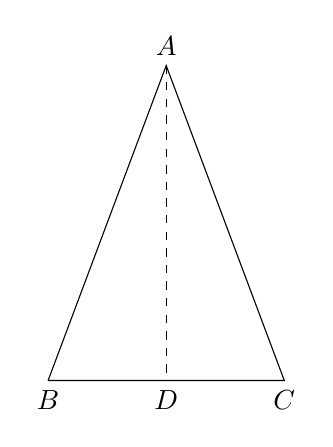
\begin{tikzpicture}
\draw (0,0)node[below]{$B$}--(3,0)node[below]{$C$}--(1.5,4)node[above]{$A$}--(0,0);
\draw[dashed](1.5,4)--(1.5,0)node[below]{$D$};
\end{tikzpicture}
    \caption{}\label{fig:3-9}
\end{figure}
\begin{proof}
作 $\angle BAC$ 的平分线 $\overline{AD}$(\cref{fig:3-9}),在 $\triangle ABD$ 和 $\triangle ACD$ 中

$\because\quad AB=AC$ (已知),$\overline{AD}=\overline{AD}$(公共边),$\angle BAD=\angle CAD$(角平分线定义)

$\therefore\quad \triangle ABD≤\triangle ACD$(SAS)

$\therefore\quad \angle B=\angle C$(全等三角形的对应角相等)。
\end{proof}


由于 $\overline{BD}=\overline{DC},\; \angle BDA=\angle CDA=\ang{90}$

因此 $AD$平分$\overline{BC}$,且$AD\perp BC$。

\begin{Deduction}{推论}
等腰三角形顶角的平分线垂直、平分底边。
\end{Deduction}

也就是说,等腰三角形的顶角平分线也是底边上的高线和中线。(\emph{三线合一})

\begin{Theorem}[等腰三角形的判定定理]{定理} 
有两个角相等的三角形是等腰三角形。
\end{Theorem}

已知:在$\triangle ABC$中,$\angle B=\angle C$(图3.10)。求证:$\overline{AB}=\overline{AC}$。

\begin{figure}
    \centering
\begin{tikzpicture}
\draw(0,0)node[left]{$B$}--(2,0)node[right]{$C$}--(1,2)node[above]{$A$}--(0,0);
\draw(4,2)node[left]{$B'$}--(6,2)node[right]{$C'$}--(5,0)node[below]{$A'$}--(4,2);
\end{tikzpicture}
    \caption{}\label{fig:3-10}
\end{figure}


\begin{proof}
    根据翻转公理,我们可以把$\triangle ABC$翻转过来,
    设顶点$A$、$B$、$C$成为$A'$、$B'$、$C'$。
    
    $\because\quad \angle B=\angle C=\angle C',\quad \angle C=\angle B=\angle B'$

    又:$\because\quad \overline{BC}=\overline{C'B'}$

    $\therefore\quad \triangle ABC\cong \triangle A'C'B'$(ASA)

    $\therefore\quad \overline{AB}=\overline{A'C'}$(全等三角形的对应边相等)。

由于$\overline{AC}=\overline{A'C'}$,$\therefore\quad \overline{AB}=\overline{AC}$(等量代换)
\end{proof}

用逻辑语句说:等腰三角形的判定定理是其性质定理的
逆定理。这两个定理我们用“充要”条件可合写成一个定理:

\begin{Theorem}{定理}
   一个三角形是等腰三角形的充要条件是这个三角形有两
个角相等。
\end{Theorem}

\begin{Definition}
三条边都相等的三角形叫做\Concept{等边三角形},也叫做\Concept{正三角形}。
\end{Definition}


同学们自己证明下面等边三角形的性质定理和判定定理。

\begin{Theorem}[等边三角形的性质定理和判定定理]{定理}
  \begin{itemize}
    \item 等边三角形的三内角相等。
    \item 三内角相等的三角形是等边三角形。
  \end{itemize}
\end{Theorem}

由等腰三角形及等边三角形的性质定理和判定定理可知,在一个三角形中,由边的相等可以推知角的相等,反过来由角的相等也可推知边的相等。下面举例说明它们在证题中的应用。

\begin{example}
已知:在图3.11中,$\overline{AB}=\overline{EB}$,$\overline{AC}=\overline{DC}$,$ADB$、$AEC$是直线。

求证:$\angle ADC=\angle AEB$。
\end{example}

\begin{analyze}
要证 $\angle ADC=\angle AEB$,只需证明 $\angle ADC=\angle A$,$\angle AEB=\angle A$; 要证明 $\angle ADC=\angle A$,$\angle AEB=\angle A$,只要知道$\overline{AC}=\overline{DC}$,$\overline{AB}=\overline{BE}$ 就行了。
\end{analyze}

\begin{proof}
在$\triangle BAE$中,$\because\quad \overline{AB}=\overline{EB}$(已知),

$\therefore\quad \angle AEB=\angle A$(等腰三角形的底角相等)。

在$\triangle CAD$中,$\because\quad \overline{AD}=\overline{DC}$(已知),

$\therefore\quad \angle ADC=\angle A$(等腰三角形的底角相等)。

$\therefore\quad \angle ADC=\angle AEB$ (等量代换)。
\end{proof}

\begin{figure}
    \begin{minipage}[t]{0.48\linewidth}
    \centering
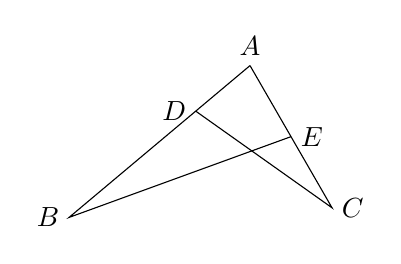
\begin{tikzpicture}[>=latex, scale=1]
\draw(40:3)node[above]{$A$}--(0,0)node[left]{$B$}--(20:3)node[right]{$E$};
\draw(40:3)--(3.34,0.122)node[right]{$C$}--(40:2.1)node[left]{$D$};
    \end{tikzpicture}
    \caption{}
    \end{minipage}
    \begin{minipage}[t]{0.48\linewidth}
    \centering
    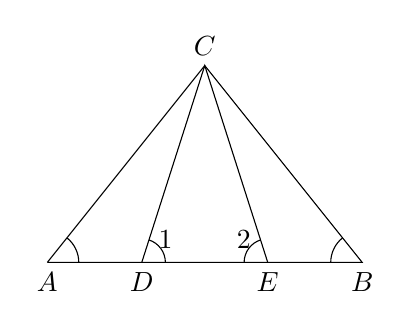
\begin{tikzpicture}[>=latex, scale=1]
\draw(-2,0)node[below]{$A$}--(0,2.5)node[above]{$C$}--(2,0)node[below]{$B$}--(-2,0);
\draw(.8,0)node[below]{$E$}--(0,2.5)--(-.8,0)node[below]{$D$};
\draw (-2+.4,0) arc (0:51.34:.4);
\draw (2-.4,0) arc (180:180-51.34:.4);
\draw (-.8+.3,0) arc (0:72.3:.3)node[right]{1};
\draw (.8-.3,0) arc (180:180-72.3:.3)node[left]{2};
    \end{tikzpicture}
    \caption{}
    \end{minipage}
    \end{figure}


\begin{example}
    如图3.12, 
己知:$\overline{AC}=\overline{BC}$,$\overline{AE}=\overline{DB}$。

求证:$\overline{CD}=\overline{CE}$。
\end{example}

\begin{analyze}
    在$\triangle CDE$中,若要证$\overline{CD}=\overline{CE}$,
   只要证$\angle 1=\angle 2$即可, $\angle 1$和$\angle 2$分别在$\triangle BCD$与$\triangle ACE$中,如能证明$\triangle BCD\cong \triangle ACE$,即可证明$\angle 1=\angle 2$。
\end{analyze}

\begin{solution}
在$\triangle ACE$与$\triangle BCD$中,

$\because\quad \overline{AC}=\overline{BC},\quad \overline{AE}=\overline{BD}$ (已知)

$\therefore\quad \angle A=\angle B$(等腰三角形两底角相等),

$\therefore\quad \triangle ACE\cong \triangle BCD$(SAS)

$\therefore\quad \angle 2=\angle 1$(全等三角形的对应角相等),

$\therefore\quad \triangle CDE$ 是等腰三角形(有两角相等的三角形是等腰三角形)。

$\therefore\quad \overline{CD}=\overline{CE}$
\end{solution}

\begin{Practice}
\begin{question}
\item\label{prac:3-2-1} 画出 $\triangle ABC$ 和 $\triangle DEF$ 的三条边上的高线。
\begin{figurehere}
  \begin{minipage}{\linewidth}\centering
    % \includegraphics{pr3-2-1.pdf}
    \caption*{第 \ref{prac:3-2-1} 题}
  \end{minipage}
\end{figurehere}
\item 画一个三角形 $ABC$,然后画出 $\triangle ABC$ 三个内角的平分线。
\item 画一个三角形 $DEF$,然后画出 $\triangle DEF$ 三边上的中线。
\item 证明:全等三角形的对应角的平分线相等。
\item 证明:全等三角形对应边上的中线相等。
\item 已知:$A=\{\text{等腰三角形}\}$,$B=\{\text{两内角相等的三角形}\}$,指出集合 $A$ 与集合 $B$ 的关系。
\item\label{prac:3-2-7} 若 $\overline{AC}=\overline{BC},\quad \angle DCA=\angle ECB$,则 $\overline{CD}=\overline{CE}$。
\item\label{prac:3-2-8} 若 $\overline{AC}=\overline{BC},\quad \angle 1=\angle 2$,则 $\overline{AE}=\overline{BD}$。
\begin{figurehere}
  \begin{minipage}[b]{0.45\linewidth}\centering
    \includegraphics{pr3-2-7.pdf}
    \caption*{第 \ref{prac:3-2-7} 题}
  \end{minipage}
  \begin{minipage}[b]{0.45\linewidth}\centering
    \includegraphics{pr3-2-89.pdf}
    \caption*{第 \ref{prac:3-2-8}--\ref{prac:3-2-9} 题}
  \end{minipage}
\end{figurehere}
\item\label{prac:3-2-9} 若 $\overline{AC}=\overline{BC}$,$\overline{AD}$、$\overline{BE}$ 分别是 $\angle A$ 和 $\angle B$ 的平分线,则 $\overline{AD}=\overline{BE}$。
\item 若 $\overline{AC}=\overline{BC},\quad \overline{AD}=\overline{BE}$,$DE$ 是直线,则 $\triangle DEC$ 是等腰三角形。
\item 若 $\overline{AC}=\overline{BC},\quad \angle ACD=\angle BCE$,$DE$ 是直线,则 $\triangle DEC$ 是等腰三角形。
\item 在等边 $\triangle ABC$ 的三边上,分别取 $D$、$E$、$F$(如图),使 $\overline{AD}=\overline{BE}=\overline{CF}$,则 $\triangle DEF$ 是等边三角形。
\item 设 $\overline{DE}=\overline{EF}=\overline{FD}$,$\angle AFD=\angle BDE=\angle CEF$,则 $\triangle ABC$ 是等边三角形。
\end{question}
\end{Practice}

\begin{figure}
    \begin{minipage}[t]{0.48\linewidth}
    \centering
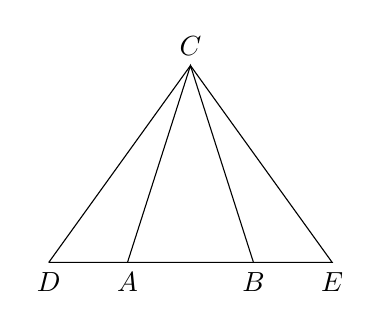
\begin{tikzpicture}[>=latex, scale=1]
    \draw(-1.8,0)node[below]{$D$}--(0,2.5)node[above]{$C$}--(1.8,0)node[below]{$E$}--(-1.8,0);
    \draw(.8,0)node[below]{$B$}--(0,2.5)--(-.8,0)node[below]{$A$};
    \end{tikzpicture}
    \caption*{第10--11题}
    \end{minipage}
    \begin{minipage}[t]{0.48\linewidth}
    \centering
    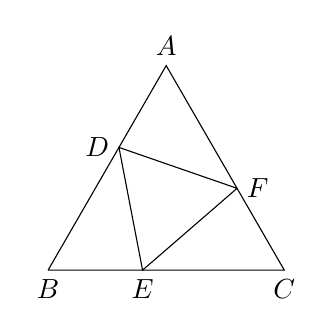
\begin{tikzpicture}[>=latex, scale=1]
\draw(-120:3)node[below]{$B$} --(0,0)node[above]{$A$}--(-60:3)node[below]{$C$}-- (-120:3) ;
\draw(-60:1.8)node[right]{$F$}--(-120:1.2)node[left]{$D$}--(-.3,-1.5*1.732)node[below]{$E$}--(-60:1.8);
    \end{tikzpicture}
    \caption*{第12--13题}
    \end{minipage}
    \end{figure}

\subsection{轴对称图形}
\begin{Definition}
在平面上有两个图形 $F$ 和 $F'$,如果平面沿着某条直线 $\ell$ 折叠起来,$F$ 和 $F'$ 叠合,就称 $F$ 和 $F'$ 关于 $\ell$ 成\Concept{轴对称}。(也称 $F$ 和 $F'$ 是以 $\ell$ 为轴的\Concept{对称形})。$F$ 和 $F'$ 上互相叠合的点叫做\Concept{对称点},$\ell$ 叫做\Concept{对称轴}。
\end{Definition}

在图3.13(1)中,平面上的 $\triangle ABC$ 和 $\triangle A'B'C'$ 关于直线 $\ell$ 成轴对称;$A$与$A'$、$B$ 与 $B'$、$C$ 与 $C'$ 都是对称点。

\begin{figure}
\begin{tikzpicture}
\begin{scope}
    \draw(0,-.5)--(0,4)node[above]{$\ell$};
    \node at (0,-1){(1)};
\draw(-1.8,2)node[above]{$B$}--(-.4,3)node[above]{$A$}--(-1.4,0.5)node[below]{$C$}--(-1.8,2);
\draw(1.8,2)node[above]{$B'$}--(.4,3)node[above]{$A'$}--(1.4,0.5)node[below]{$C'$}--(1.8,2);
\end{scope}
\begin{scope}[xshift=6.5cm]
    \draw(0,-.5)--(0,4)node[above]{$\ell$};
\draw(-2,0)node[below]{$B$}--(2,0)node[below]{$C$}--(0,3)node[right]{$A$}--(-2,0);
\draw (0,0) rectangle (.2,.2);
\node at (0,-1){(2)};
\end{scope}
\end{tikzpicture}
    \caption{}\label{fig:3-13}
\end{figure}

\begin{Deduction}{推论}
两个图形如果关于某直线成轴对称,那么这两个图形是全等形。
\end{Deduction}

\begin{Definition}
如果一个图形可以分成两部分,这两部分关于某一直线成轴对称,就把这个图形称为\Concept{轴对称形}。
\end{Definition}

显然,等腰三角形关于它的顶角平分线成轴对称图形图3.13(2))。轴对称形在实际中应用非常广泛,图3.14中的图形,都是轴对称形。
\begin{figure}
% \includegraphics[scale=.6]{fig/3-14.png}
    \caption{}\label{fig:3-14}
\end{figure}

轴对称图形有什么性质呢?这就要研究一下对称轴和对称点的关系。

在图3.15中,设 $A$ 与 $A'$ 是关于直线 $\ell$ 的轴对称点,因为 $A$、$A'$和$\ell$在同一平面内,并且 $A$ 和 $A'$ 在 $\ell$ 的两侧,所以线段 $\overline{AA'}$ 与 $\ell$ 必相交,设交点为 $O$,在 $\ell$ 上取异于 $O$的另一点$P$,连结 $\overline{AP}$,$\overline{A'P}$。

由于 $A$ 点所在的半平面沿直线 $\ell$ 折叠过来,$A$ 和 $A'$ 重合,而 $\ell$ 上的 $P$ 和 $O$ 重合于自身,所以$\overline{AP}=\overline{A'P}$,$\angle APO=\angle A'PO$,$\triangle PAA'$是等腰三角形,直线$\ell$是顶角的平分线,
所以 $\ell$ 垂直平分底边 $\overline{AA'}$。

由此得出轴对称图形的重要性质:
\begin{enumerate}
  \item 对称轴上的任一点,与每一双对称点的距离相等。
  \item 对称轴是每一双对称点所连线段的垂直平分线。
\end{enumerate}

在上述性质的证明中,我们所取 $P$ 点异于 $O$,如果 $P$ 点就是 $O$ 点,结论仍然一样。

由于一条线段的垂直平分线是唯一的,由性质2可知,如果 $\overline{AA'}$ 的垂直平分线是 $\ell$,那么 $A$ 与 $A'$ 是以 $\ell$ 为轴的对称点。

由此,我们就可以作出已知图形以某直线为轴的对称形。

\begin{figure}
    \begin{minipage}[t]{0.48\linewidth}
    \centering
\begin{tikzpicture}[>=latex, scale=.8]
    \draw(0,-.5)--(0,4)node[above]{$\ell$};
\draw(-2,0)node[below]{$A$}--(2,0)node[below]{$A'$}--(0,3)node[right]{$P$}--(-2,0);
\draw (0,0)node[below right]{$O$} rectangle (.2,.2);
    \end{tikzpicture}
    \caption{}
    \end{minipage}
    \begin{minipage}[t]{0.48\linewidth}
    \centering
    \begin{tikzpicture}[>=latex, scale=1]
% \draw(0,-.5)--(0,4)node[above]{$\ell$};     
% \tkzDefPoints{-1/3/A, 1/3/A', -2.5/2/B,2.5/2/B',-1.5/0/C,1.5/0/C',-.5/.8/D, .5/.8/D'}
% \tkzDrawPolygon(A,B,C,D)\tkzDrawPolygon(A',B',C',D')
% \foreach \x in {A,B,C,D}
% {
%     \draw(\x)--(\x');
% }
% \tkzDefPoints{0/2.1/O}
% \tkzAutoLabelPoints[center=O](A,B,C,D,A',B',C',D')
% \node at (0,3)[below right]{$O$};
% \draw(0,3) rectangle (-.2,3+.2);
    \end{tikzpicture}
    \caption{}
    \end{minipage}
    \end{figure}



\begin{example}
已知:四边形$ABCD$及直线$\ell$。(图3.16)

求作:四边形$ABCD$以$\ell$为轴的轴对称形。

作法:
\begin{enumerate}
\item 由$A$点引$\ell$的垂线交$\ell$于$O$点,在射线$AO$上
取$OA'=AO$,则$A'$是$A$点关于轴$\ell$的对称点。
\item 用同样的方法作点$B$、$C$、$D$关于$\ell$的对称点$B'$、
$C'$、$D'$。
\item 连结$\overline{A'B'}$,$\overline{B'C'}$,$\overline{C'D'}$,$\overline{D'A'}$,则四边形
$A'B'C'D'$就是四边形$ABCD$以$\ell$为轴的轴对称图形。
\end{enumerate}

为什么呢?因为根据作法,如果把四边形 $ABCD$ 和四边形 $A'B'C'D'$ 所在平面,沿直线$\ell$折叠起来,则 $A$ 与 $A'$、
$B$与$B'$、$C$与$C'$、$D$与$D'$分别重合,所以四边形$ABCD$与
四边形$A'B'C'D'$完全重合,所以这两个四边形是以$\ell$为轴
的对称图形。
\end{example}

\begin{example}
    有公共底的两个等腰三角形,通过底所对的两个顶点的直线是它们所组成图形的对称轴。

已知:在图3.17中,$BC$是等腰$\triangle ABC$与等腰$\triangle A'BC$
的公共底边。

求证:直线$AA'$是这个图形的对称轴。
\end{example}

\begin{figure}
    \centering
\begin{tikzpicture}[scale=.8]
\begin{scope}
\draw(0,-1.5)--(0,4);
\draw(-1.5,0)node[left]{$B$}--(1.5,0)node[right]{$C$}--(0,3)node[right]{$A$}--(-1.5,0)--(0,-1)node[right]{$A'$}--(1.5,0);

\end{scope}
\begin{scope}[xshift=7cm]
    \draw(0,-1)--(0,4);
\draw(-1.5,0)node[left]{$B$}--(1.5,0)node[right]{$C$}--(0,3)node[right]{$A$}--(-1.5,0)--(0,1.8)node[right]{$A'$}--(1.5,0);

\end{scope}
\end{tikzpicture}
    \caption{}
\end{figure}

\begin{proof}
$\because\quad \overline{AB}=\overline{AC},\quad \overline{A'B}=\overline{A'C}$(已知)

$\therefore\quad \angle ABC=\angle ACB,\quad 
\angle A'BC=\angle A'CB$(等腰三角形的两底角相等)。

两式相加(或相减)得:
$\angle ABA'=\angle ACA'$(等量加(或减)等量其和(或差)
相等)。

$\therefore\quad \triangle ABA'\cong \triangle ACA'$(SAS)

以$AA'$为轴折叠起来,$\triangle ABA'$与$\triangle ACA'$能够重
合,所以$AA'$是这个图形的对称轴。
\end{proof}

\begin{example}
    证明四条边相等的四边形的两条对角线互相垂直
平分,并且平分一双对角。

已知:在四边形$ABCD$中,$\overline{AB}=\overline{BC}=\overline{CD}=\overline{DA}$。
(图3.18)
\begin{figure}
    \centering
    \begin{tikzpicture}
    \draw(-2,0)--(0,1.2)--(2,0)--(0,-1.2)--(-2,0);
    \draw(-2,0)node[above]{$B$}--(2,0)node[above]{$D$};
    \draw(0,1.2)node[above]{$A$}--(0,-1.2)node[below]{$C$};
    \node at (0,0)[below right]{$O$};        
    \end{tikzpicture}
    \caption{}
\end{figure}

求证:$AC$、$BD$互相垂直平分,且$AC$平分$\angle A$和$\angle C$,
$BD$平分$\angle B$和$\angle D$。
\end{example}

\begin{proof}
在四边形$ABCD$中,
因为$\overline{AB}=\overline{BC}=\overline{CD}=\overline{DA}$,所
以四边形$ABCD$可看成由两个
等腰三角形所拼成:等腰$\triangle ABD$
与等腰$\triangle CBD$,或等腰$\triangle ABC$
与等腰$\triangle ADC$。由例3.8可知,
对角线$\overline{AC}$、$\overline{BD}$所在的直线都是四边形$ABCD$的对称
轴。所以,$\overline{AC}$、$\overline{BD}$互相垂直平分,并且$\overline{AC}$平分$\angle A$和
$\angle C$,$\overline{BD}$平分$\angle B$和$\angle D$。
\end{proof}

\begin{Practice}
\begin{question}
  \item 下列各图形有多少个对称轴?对称轴是什么?
  \begin{tasks}(3)
    \task 线段;
    \task 射线;
    \task 直线。
  \end{tasks}
  \item 已知直线 $\ell$ 和 $\ell$ 外面一点 $A$,只用圆规和直尺求作点 $A$ 以直线 $\ell$ 为对称轴的对称点 $A'$。
  \item 求作两个已知点的对称轴。
  \item 已知 $\triangle ABC$ 和直线 $\ell$,作 $\triangle ABC$ 以 $\ell$ 为对称轴的对称形。
  \item 求作与已知等边三角形 $ABC$ 分别以 $AB$、$AC$、$BC$ 为对称轴的对称图形。
  \item 作图。(只要求作出图形)
  \begin{tasks}(2)
    \task 画已知线段 $\overline{AB}$ 的对称轴。
    \task 画已知 $\angle A$ 的对称轴。
  \end{tasks}
  \item 等腰三角形有几个对称轴?等边三角形有几个对称轴?任画一个等边三角形把它的对称轴都画出来。
\end{question}
\end{Practice}

\subsection{三角形中的不等关系}
\begin{Definition}
    和三角形的内角相邻并且和它互补的角叫做三角
形的\Concept{外角}。
\end{Definition}
 
如图3.19中的$\angle ACD$
就是$\triangle ABC$的一外个角。
这时$\angle ACB$称为$\angle ACD$
相邻的内角,$\angle A$和$\angle B$
分别称为$\angle ACD$不相邻的内角。

\begin{Theorem}{定理}
 三角形的外角大于和它不相邻的任一内角。
\end{Theorem}

\begin{figure}
    \begin{minipage}[t]{0.48\linewidth}
    \centering
\begin{tikzpicture}[>=latex, scale=1]
\draw(0,0)node[left]{$B$}--(4.5,0)node[right]{$D$};
\draw(3,0)node[below]{$C$}--(1.7,2)node[above]{$A$}--(0,0);
\draw(3.4,0) arc (0:120:.4);
    \end{tikzpicture}
    \caption{}
    \end{minipage}
    \begin{minipage}[t]{0.48\linewidth}
    \centering
    \begin{tikzpicture}[>=latex, scale=1]
\draw(0,0)node[left]{$A$}--(3,0)node[below]{$B$};
\draw[dashed](3,0)--(4.5,0)node[right]{$D$};
\draw(3,0)--(1.7,2)node[above]{$C$}--(0,0);
\draw[dashed](3,0)--(4.7,2)node[right]{$F$}--(0,0); 
\node at (2.35,1)[above]{$E$};
    \end{tikzpicture}
    \caption{}
    \end{minipage}
    \end{figure}

已知:$\triangle ABC$和外角
$\angle CBD$(图3.20)。

求证:$\angle CBD>\angle C$
或$\angle A$。

\begin{proof}
    假定$E$是$\overline{BC}$
中点,引$AE$并延长到$F$,
使$\overline{EF}=\overline{AE}$,作$\overline{BF}$。

在$\triangle ACE$和$\triangle FBE$中,

$\because\quad \overline{AE}=\overline{EF}$ (作图),

$\because\quad E$是$\overline{BC}$中点(假定),

$\therefore\quad \overline{CE}=\overline{EB}$(线段中点定义),

$\because\quad \angle CEA=\angle BEF$(对顶角相等),

$\therefore\quad \triangle ACE\cong \triangle FBE$ (SAS),

$\therefore\quad \angle EBF=\angle C$(全等三角形的对应角相等)。

由于$\angle CBD>\angle EBF$ (全量大于它的任何一部分)。

$\therefore\quad \angle CBD>\angle C$ (等量代换)。

同理可证 $\angle CBD> \angle A$。
\end{proof}

\begin{Theorem}{定理}
 在一个三角形中,如果两条边不等,那么它们所
对的角也不等,大边所对的角较大;反之,如果在一个三角
形中两个角不等,那么它们所对的边也不等。大角所对的边
较大。
\end{Theorem}

已知:$\triangle ABC$(图3.21)

\begin{figure}
    \begin{minipage}[t]{0.48\linewidth}
    \centering
\begin{tikzpicture}[>=latex, scale=1.3]
% \tkzDefPoint(0,0){A}
% \tkzDefPoint(-50:2){C}
% \tkzDefPoint(-120:2){D}
% \tkzDefPoint(-120:3){B}
% \tkzDefPoint(0,-1.5){O}
% \tkzDrawPolygon(A,C,B)
% \draw[dashed](D)--(C);
% \tkzMarkAngles[mark=none, size=.3](C,D,A A,C,D)
% \tkzLabelAngle[pos=.6](C,D,A){2}
% \tkzLabelAngle[pos=.6](A,C,D){1}
% \tkzAutoLabelPoints[center=O](A,C,B,D)       
    \end{tikzpicture}
    \caption{}
    \end{minipage}
    \begin{minipage}[t]{0.48\linewidth}
    \centering
    \begin{tikzpicture}[>=latex, scale=1.3]
% \tkzDefPoint(0,0){A}
% \tkzDefPoint(30:1.5){D}
% \tkzDefPoint(-150:2){B}
% \tkzDefPoint(-30:1.5){C}
% \tkzDrawPolygon(A,C,B)
% \draw[dashed](A)--(D)--(C);
% \tkzMarkAngles[mark=none, size=.2](D,C,A A,D,C)
% \tkzLabelAngle[pos=.4](A,D,C){2}
% \tkzLabelAngle[pos=.4](D,C,A){1}
% \tkzAutoLabelPoints[center=A](C,B,D)  
% \node at (0,0)[above left]{$A$};
    \end{tikzpicture}
    \caption{}
    \end{minipage}
    \end{figure}

求证:
\begin{enumerate}
    \item $\overline{AB}>\overline{AC}\quad \Rightarrow\quad \angle C>\angle B$
    \item $\angle C>\angle B\quad \Rightarrow\quad \overline{AB}>\overline{AC}$
\end{enumerate}

\begin{proof}
    先证$\overline{AB}>\overline{AC}\quad\Rightarrow\quad \angle C>\angle B$。

在$AB$上截$\overline{AD}=\overline{AC}$,
则$\triangle ADC$为等腰三角形。

$\therefore\quad \angle 1=\angle 2$。

由于$\angle ACB>\angle 1$ (不等量基本性质6)

$\therefore\quad \angle ACB>\angle 2$(等量代换)。

但$\angle 2>\angle B$ (三角形的外角大于和它不相邻的任一内
角),

$\therefore\quad \angle ACB>\angle B$(不等量基本性质5)

即:$\angle C>\angle B$。

我们再证$\angle C>\angle B\quad \Rightarrow\quad \overline{AB}>\overline{AC}$

如果$\overline{AB}$不大于$\overline{AC}$,那么$\overline{AB}=\overline{AC}$或$\overline{AB}<\overline{AC}$。
若$\overline{AB}=\overline{AC}$,则$\angle B=\angle C$,若$\overline{AB}<\overline{AC}$,则$\angle C<\angle B$,这两
种结果都和$\angle C>\angle B$矛盾。

$\therefore\quad \angle C>\angle B\quad \Rightarrow\quad \overline{AB}>\overline{AC}$
\end{proof}

\begin{Theorem}{定理}
    三角形任意两边之和大于第三边。
\end{Theorem}
 
已知:$\triangle ABC$(图3.23)。

求证:$\overline{AB}+\overline{AC}>\overline{BC}$。

\begin{proof}
    在$BA$的延长线上取一点$D$,使$AD=AC$。则
    $\triangle ACD$为等腰三角形。
  
    $\therefore\quad \angle 1=\angle 2$

    $\because\quad \angle BCD>\angle 1$(不等量
    基本性质6)

$\therefore\quad \angle BCD>\angle 2$(等量代
    换)。

    在$\triangle BCD$中,由前面的定理可知:
    $\overline{BD}>\overline{BC}$,但$\overline{BD}=\overline{AB}+\overline{AD}=\overline{AB}+\overline{AC}$,
 
   $\therefore\quad  \overline{AB}+\overline{AC}>\overline{BC}$
\end{proof}

\begin{Deduction}{推论}
三角形任一边大于其他两边之差。
\end{Deduction}

下面我们举例说明上述定理的一些应用。


\begin{example}
    已知:$\triangle ABC$中$\overline{AB}=\overline{AC}$,$D$点在$\overline{BC}$上,$E$点
在$\overline{BC}$的延长线上(图3.23)。

求证:$\overline{AD}<\overline{AB}<\overline{AE}$
\end{example}

\begin{figure}
    \begin{minipage}[t]{0.48\linewidth}
    \centering
\begin{tikzpicture}[>=latex, scale=1]
%     \tkzDefPoints{0/1.5/A, -1.5/-1/B, -.25/-1/D, 1.5/-1/C, 2.5/-1/E}
% \tkzDrawPolygon(A,C,B)
%     \draw(D)node[below]{$D$}--(A)node[above]{$A$}--(E)node[below]{$E$};
% \draw[dashed](C)--(3.5,-1);
% \node at (B)[below]{$B$};
% \node at (C)[below]{$C$};
% \tkzMarkAngles[mark=none, size=.3](D,B,A  A,D,B  A,C,B)
% \tkzLabelAngle[pos=.5](D,B,A){1}
% \tkzLabelAngle[pos=.5](A,D,B){3}
% \tkzLabelAngle[pos=.5](A,C,B){2}
    \end{tikzpicture}
    \caption{}
    \end{minipage}
    \begin{minipage}[t]{0.48\linewidth}
    \centering
    \begin{tikzpicture}[>=latex, scale=1.2]
% \tkzDefPoint(0,0){D}
% \tkzDefPoint(-60:2){C}
% \tkzDefPoint(180-60:1){A}
% \tkzDefPoint(-140:1.2){E}
% \tkzDefPoint(-140:2.8){B}
% \tkzDrawPolygon(A,C,B)
% \draw(B)--(E)--(C);
% \draw[dashed](E)--(D);
% \foreach \x in {A,D,C}
% {
%     \node at (\x) [right]{ $\times$ };
% }
% \foreach \x in {B,E}
% {
%     \node at (\x) [left]{ $\times$ };
% }
% \tkzMarkAngles[mark=none, size=.2](E,D,C)
% \tkzLabelAngle[pos=.4](E,D,C){1}
    \end{tikzpicture}
    \caption{}
    \end{minipage}
    \end{figure}

\begin{proof}
$\because\quad \overline{AB}=\overline{AC}$

$\therefore\quad \angle 1=\angle 2$

又$\because\quad \angle 3>\angle 2$

$\therefore\quad \angle 3>\angle 1$

$\therefore\quad \overline{AB}>\overline{AD}$(在一个三角形中,大角对大边。)

又:$\because\quad \angle 2>\angle E$

$\therefore\quad \angle 1>\angle E$

$\therefore\quad \overline{AE}>\overline{AB}$(在一个三角形中,大角对大边。)

因此有:$\overline{AD}<\overline{AB}<\overline{AE}$
\end{proof}


\begin{example}
    已知:$E$点在$\triangle ABC$内(图3.24)。

求证: \begin{enumerate}
    \item $\angle BEC>\angle A$
    \item $\overline{BE}+\overline{EC}<\overline{AB}+\overline{AC}$
\end{enumerate} 
\end{example}

\begin{proof}
    延长$\overline{BE}$交$\overline{AC}$于$D$点,
则$\angle BEC>\angle 1$,$\angle BEC>\angle 1$

$\therefore\quad \angle BEC>\angle A$(不等量基
本性质5)。

又$\because\quad \overline{BE}+\overline{ED}<\overline{AD}+\overline{AB}$,$\overline{EC}<\overline{ED}+\overline{DC}$(三角形两边之和大于第三边)。

$\therefore\quad \overline{BE}+\overline{ED}+\overline{EC}<\overline{AD}+\overline{AB}+\overline{ED}+\overline{DC}$(不等量基本性质3)。

$\therefore\quad \overline{BE}+\overline{EC}<\overline{AB}+\overline{AC}$(不等量基本性质1)。
\end{proof}

\begin{example}
如图3.25所示,$A$、$B$是平面上直线$\ell$同侧的两点,试在直线$\ell$上求一点$P$,使$\overline{AP}+\overline{PB}$最短。

在没有作这题前,让我们想一想该怎样着手,我们要求$\overline{AP}+\overline{PB}$最短,但怎样才能最短呢?

我们知道两点间的直线段最短,但是我们却要在$\ell$上求一点,使$\overline{AP}+\overline{PB}$最短。如果$A,B$两点在$\ell$的两侧,那么问题要简单得多(作$\overline{AB}$与$\ell$交于$P$,$P$点就是所求的点)。但我们曾学过,如果两点是轴对称点,那么它们的对称轴就是两点间线段的垂直平分线,并且对称轴上的点到两对称点的距离相等。我们只要作出$A$点关于轴$\ell$的对称点$A'$,我们求$\overline{AP}+\overline{PB}$的最小值,就可转化为求$\overline{A'P}+\overline{PB}$的最小值了。而$A'$、$B$两点在$\ell$的异侧,这是很容易的。

\begin{figure}
\begin{tikzpicture}[xscale=.6, rotate=5]
\draw (-2,0)--(8,0)node[right]{$\ell$};
\draw[dashed](-.5,1)node[left]{$A$}--(-.5,-1)node[left]{$A'$};
\draw[dashed](-.5,-1)--(5.5,2)node[right]{$B$};
\draw[very thick](-.5,1)--(1.5,0)node[below]{$P$}--(5.5,2);
\node at (-.5,0)[below left]{$D$};
\draw[dashed](-.5,1)  -- (6.5,0) node[below]{$C$}--(-.5,-1);
\draw[dashed](5.5,2)  -- (6.5,0);
\end{tikzpicture}
    \caption{}
\end{figure}
\end{example}


\begin{solution}
    作$A$点关于轴$\ell$的对称点$A'$,作$\overline{A'B}$与$\ell$相交于$P$,
    则$P$点使$\overline{AP}+\overline{PB}$最短。因为,如果在$\ell$上任找另外一点$C$,
    在$\triangle A'BC$中,
    $\overline{A'B}<\overline{A'C}+\overline{CB}$(三角形两边之和大于第三边),
    但$\overline{A'B}=\overline{A'P}+\overline{PB}$

将    $\overline{A'P}=\overline{AP},\quad \overline{A'C}=\overline{AC}$ 代入上式,
    则得:$\overline{AP}+\overline{PB}<\overline{AC}+\overline{CB}$。

    这就证明了$P$点使$\overline{AP}+\overline{PB}$最短。
\end{solution}

\begin{rmk}
    如果$\ell$是镜子的话,那么从$A$点发出的光线,若反
射到$B$点,那么$\overline{AP}$、$\overline{PB}$就是光所走的路线。因为光线总是
走最近的路,在光学中就有:“入射角等于反射角”这条定
律。即$\angle APD=\angle BPC$。在光学中由观测得到的结果和我
们用数学定理得出的结果一致。在自然界中我们有能力观测
到的结论是有限的,如何由这些有限的可观测的结论,得到
更进一步的结论,甚至有些是观测不到的结论,我们需要数
学这样有力的工具。
\end{rmk}
    
\begin{Practice}
\begin{question}
  \item 已知:如图,$\triangle ABC$ 内有一点 $P$,求证:$\angle BPC>\angle BAC$。
  \item 已知:如图,$\triangle ABC$ 内有一点 $P$,求证:$\overline{AB}+\overline{AC}>\overline{PB}+\overline{PC}$。
  \item 将金属丝弯成三角形,如果要求一边长是 \qty{25}{cm},那么金属丝至少大于多少 \unit{cm} 才能作成三角形?
  \item 证明四边形两条对角线之和小于周长而大于半周长。
  \item 证明三角形的一边小于它的周长的一半。
  \item 用整数表示三角形的各边,一边是 \qty{3}{m},另一边是 \qty{2}{m},第三边可以是多少米?
  \item 在平面上 $\overline{AB}$ 的垂直平分线的 $A$ 点的一侧取一点 $P$,那么 $\overline{PA}$ 和 $\overline{PB}$ 哪一条线段长?
  \item 已知:如图,$\triangle ABC$ 中,$\angle A>\angle C$,$D$、$E$ 分别在 $\overline{AB}$、$\overline{AC}$ 上并且 $\overline{AD}>\overline{AE}$。求证:
  \begin{tasks}
    \task $\angle BDE> \angle CED$
    \task $\overline{BC}>\overline{BE}$
  \end{tasks}
\end{question}
\end{Practice}
    
\begin{figure}
    \begin{minipage}[t]{0.48\linewidth}
    \centering
\begin{tikzpicture}[>=latex, scale=1]
%     \tkzDefPoint(-60:2){C}
%     \tkzDefPoint(180-60:1){A}
%     \tkzDefPoint(-140:2.8){B}
%     \tkzDefPoint(-.25,-.5){P}
%     \tkzDrawPolygon(A,C,B)
%     \draw(B)--(P)--(C);
% \tkzAutoLabelPoints[center=P](A,B,C)
% \node at (P)[above]{$P$};
    \end{tikzpicture}
    \caption*{第1--2题}
    \end{minipage}
    \begin{minipage}[t]{0.48\linewidth}
    \centering
    \begin{tikzpicture}[>=latex, scale=1.3]
        % \tkzDefPoint(0,0){A}
        % \tkzDefPoint(-45:2){C}
        % \tkzDefPoint(-45:1){E}
        % \tkzDefPoint(-140:2.8){B}
        % \tkzDefPoint(-140:2){D}
        % \tkzDrawPolygon(A,C,B)
        % \tkzDrawPolygon(D,B,E)
        % \tkzDefPoint(.1,-1){O}
        % \tkzAutoLabelPoints[center=O](A,B,C,D,E)
    \end{tikzpicture}
    \caption*{第8题}
    \end{minipage}
    \end{figure}

\section*{习题3.1}
\addcontentsline{toc}{subsection}{习题3.1}
\begin{enumerate}
    \item 已知:如图,$\overline{AD}=\overline{AE}$,$\overline{BD}=\overline{EC}$,
    求证:$\overline{DO}=\overline{EO}$。
    \item 已知:如图,$\overline{AB}=\overline{AD}$,$AC$平分$\angle BAD$,$E$是$\overline{AC}$上一点。
    求证:$\angle EBC=\angle EDC$。
    \item 求证:等腰三角形两腰上的中线相等。
    \item 已知:如图,$\angle B=\angle C$,$\overline{BD}=\overline{EC}$。
    求证:$\angle 1=\angle 2$。

\begin{figure}
    \begin{minipage}[t]{0.31\linewidth}
    \centering
\begin{tikzpicture}[>=latex, scale=1]
% \tkzDefPoints{-1.5/0/B, 1.5/0/C, -.5/2/D, .5/2/E, 0/3/A}
% \tkzDrawPolygon(A,B,C)
% \tkzDrawSegments(B,E C,D)
% \tkzInterLL(C,D)(B,E)  \tkzGetPoint{O}
% \tkzLabelPoints[left](B,D)
% \tkzLabelPoints[right](C,E)
% \tkzLabelPoints[above](A)
% \tkzLabelPoints[below](O)


    \end{tikzpicture}
    \caption*{第1题}
    \end{minipage}
    \begin{minipage}[t]{0.31\linewidth}
    \centering
    \begin{tikzpicture}[>=latex, scale=1]
% \tkzDefPoints{-1.5/0/B, 1.5/0/D, 0/1.5/A, 0/-2/C, 0/.8/E}
% \tkzDrawPolygon(A,B,C,D)
% \tkzDrawSegments(B,E A,C E,D)
% \tkzLabelPoints[left](B)
% \tkzLabelPoints[right](D)
% \tkzLabelPoints[above](A)
% \tkzLabelPoints[below](C)
% \tkzLabelPoints[below right](E)
    \end{tikzpicture}
    \caption*{第2题}
    \end{minipage}
        \begin{minipage}[t]{0.31\linewidth}
    \centering
    \begin{tikzpicture}[>=latex, scale=1]
% \tkzDefPoints{-1.5/0/B, 1.5/0/C, -.75/0/D, .75/0/E, 0/3/A}
% \tkzDrawPolygon(A,B,C)
% \tkzDrawSegments(A,E A,D)
% \tkzLabelPoints[left](B)
% \tkzLabelPoints[right](C)
% \tkzLabelPoints[above](A)
% \tkzLabelPoints[below](D,E)
% \tkzMarkAngles[mark=none, size=.3](C,D,A A,E,B)
% \tkzLabelAngle[pos=.5](C,D,A){1}
% \tkzLabelAngle[pos=.5](A,E,B){2}
    \end{tikzpicture}
    \caption*{第4题}
    \end{minipage}
    \end{figure}

    \item 已知:如图,在四边形$ABCD$中,
    $\overline{AD}=\overline{AB}$,$\overline{CD}=\overline{BC}$
    
    求证:$\angle 1=\angle 2$;$\angle 3=\angle 4$;$AC\perp DB$
  
    \item 如图,已知:$\angle 1=\angle 2$,$\angle 3=\angle 4$,
求证:$\overline{AB}=\overline{AC}$。
\item 如图,已知:$\overline{BE}=\overline{ED}$,$\angle 1=\angle 2$。
求证:$\overline{AB}=\overline{CD}$。

\begin{figure}
    \begin{minipage}[t]{0.48\linewidth}
    \centering
\begin{tikzpicture}[>=latex, scale=1]
    % \tkzDefPoints{-2/0/A, 2/0/C, -1/1.5/D, -1/-1.5/B, -1/0/E}
    % \tkzDrawPolygon(A,B,C,D)
    % \tkzLabelPoints[left](A)
    % \tkzLabelPoints[right](C)
    % \tkzLabelPoints[above](D)
    % \tkzLabelPoints[below](B)
    % \tkzLabelPoints[above right](E)
    % \tkzDrawSegments(A,C D,B)
    % \tkzMarkAngles[mark=none, size=.4](C,A,D D,C,A)
    % \tkzMarkAngles[mark=none, size=.5](B,A,C A,C,B)
    % \tkzLabelAngle[pos=.7](C,A,D){1}
    % \tkzLabelAngle[pos=.7](B,A,C){2}
    % \tkzLabelAngle[pos=.7](D,C,A){3}
    % \tkzLabelAngle[pos=.7](A,C,B){4}

    \end{tikzpicture}
    \caption*{第5题}
    \end{minipage}
    \begin{minipage}[t]{0.48\linewidth}
    \centering
    \begin{tikzpicture}[>=latex, scale=1]
        % \tkzDefPoints{-1.5/0/B, 1.5/0/C, 0/3.5/A, 0/1/O}
        % \tkzDrawPolygon(A,B,C)
        % \tkzLabelPoints[left](B)
        % \tkzLabelPoints[right](C)
        % \tkzLabelPoints[above](A)
        % \tkzLabelPoints[below](O)
        % \tkzDrawSegments(A,O B,O C,O)        
        % \tkzMarkAngles[mark=none, size=.4](C,B,O O,C,B)
        % \tkzMarkAngles[mark=none, size=.3](A,O,B)
        % \tkzLabelAngle[pos=.6](C,B,O){1}
        % \tkzLabelAngle[pos=.6](O,C,B){2}
        % \tkzLabelAngle[pos=.5](A,O,B){3}
        % \tkzMarkAngles[mark=none, size=.35](C,O,A)
        % \tkzLabelAngle[pos=.5](C,O,A){4}

    \end{tikzpicture}
    \caption*{第6题}
    \end{minipage}
    \end{figure}

\item 在 $\triangle ABC$ 中,$\overline{AB}=\overline{AC}$,$D$、$E$ 两点分别在 $\overline{AB}$ 和 $\overline{AC}$ 上,且 $\overline{BE}$
和$\overline{CD}$交于$O$点,$\overline{BD}=\overline{CE}$。求证:$AO$平分$\angle BAC$。
\item 在$\triangle ABC$中,$D$为$\overline{BC}$延长线上一点,且$\overline{CD}=\overline{AC}$,$F$
是
$\overline{AD}$中点,$\overline{CE}$是$\angle ACB$的平分线。求证$CE\perp CF$。

\item 在$\triangle ABC$中,$\angle B=2\angle C$,$AD$平分$\angle A$,交$\overline{BC}$于$D$点,
求证:$\overline{AB}+\overline{BD}=\overline{AC}$。

\begin{figure}
    \begin{minipage}[t]{0.48\linewidth}
    \centering
\begin{tikzpicture}[>=latex, scale=1]
    % \tkzDefPoints{-1.5/0/A, 1.5/0/C, -1/2/B, 1/2/D}
    % \tkzDrawPolygon(A,B,C)
    % \tkzDrawPolygon(A,D,C)
    % \tkzInterLL(B,C)(A,D) \tkzGetPoint{E}
    % \tkzLabelPoints[left](A)
    % \tkzLabelPoints[right](C)
    % \tkzLabelPoints[above](B,D,E)
    % \tkzMarkAngles[mark=none, size=.4](B,C,A C,A,D)
    % \tkzLabelAngle[pos=.6](C,A,D){1}
    % \tkzLabelAngle[pos=.6](B,C,A){2}
    \end{tikzpicture}
    \caption*{第7题}
    \end{minipage}
    \begin{minipage}[t]{0.48\linewidth}
    \centering
    \begin{tikzpicture}[>=latex, scale=1]
% \tkzDefPoints{0/0/B, 3/0/C, 3/1.5/D}
% \tkzDefPoint(70:3){A}
% \tkzDrawPolygon(A,B,C,D)
% \tkzLabelPoints[below](B,C)
% \tkzLabelPoints[above](A,D)
    \end{tikzpicture}
    \caption*{第11题}
    \end{minipage}
    \end{figure}

\item 如图,已知四边形$ABCD$中,
$\overline{AB}=\overline{BC}$,$\overline{AD}>\overline{CD}$。

求证:$\angle BCD>\angle BAD$。
\item 已知:$\triangle ABC$中,$D$是$\overline{AC}$上
一点,且$\overline{BD}>\overline{BC}$。

求证:$\overline{AB}>\overline{AC}$。
\item 三角形的一边等于2米,另一边等于8米,如果已知第三边能用被3整除的整数表示,求第三边。
\item 已知:$\triangle ABC$在平面$\alpha$上,点$P\in\alpha$,并且$P$在$\triangle ABC$的外部

求证:$\overline{PA}+\overline{PB}+\overline{PC}>\frac{1}{2}(\overline{AB}+\overline{BC}+\overline{AC})$
\item 已知:$\triangle ABC$在平面$\alpha$上,点$P\in\alpha$,并且$P$在$\triangle ABC$的内部

求证:$\overline{PA}+\overline{PB}+\overline{PC}<\overline{AB}+\overline{BC}+\overline{AC}$。
\item 求证:三角形一边上的中线小于其他两边和的一半。
\item 在两条公路$OX$和$OY$上,分别设邮筒$A$和$B$,邮递员每天由邮局$P$到邮筒$A$、$B$取信,然后返回邮局。问$A$、$B$的位置确定在哪儿,才能使邮递员走的路程最短?

\begin{figure}[htbp]
    \centering
\begin{tikzpicture}
% \tkzDefPoints{-2/0/X, 2/0/Y, .5/3/X1, -.5/3/Y1, 0/0/P}
% \tkzDefPointWith[linear, K=.5](X,X1) \tkzGetPoint{A}
% \tkzDefPointWith[linear, K=.3](Y,Y1) \tkzGetPoint{B}
% \tkzDrawPolygon(A,B,P)
% \tkzInterLL(X,X1)(Y,Y1)  \tkzGetPoint{O}
% \tkzDrawSegments(X,X1 Y,Y1)
% \tkzLabelPoints[below](X,Y,P)
% \tkzLabelPoints[left](A)
% \tkzLabelPoints[right](B,O)
\end{tikzpicture}
    \caption*{第17题}
\end{figure}
\end{enumerate}

\section{平行线与内角和定理}

\subsection{平行线}
\begin{Definition}
平面上两条直线被第三条直线所截,截得八个
角,如图3.26, 其中的$\angle 1$和$\angle 5$,$\angle 4$和$\angle 8$,$\angle 2$和$\angle 6$,
$\angle 3$和$\angle 7$,都叫做\Concept{同位角},$\angle 4$和$\angle 6$,$\angle 3$和$\angle 5$都叫\Concept{内错
角},$\angle 4$和$\angle 5$,$\angle 3$和$\angle 6$都叫做\Concept{同旁内角}。
\end{Definition}

\begin{figure}
    \begin{minipage}[t]{0.48\linewidth}
    \centering
\begin{tikzpicture}[>=latex, scale=1]
% \tkzDefPoints{-2/2/A, 2/2.5/B, -2/0/C, 2/1.5/D, 0/-.5/F, 0/4/E}
% \tkzDrawSegments(A,B C,D E,F)
% \tkzInterLL(A,B)(E,F)  \tkzGetPoint{P}
% \tkzInterLL(C,D)(E,F)  \tkzGetPoint{Q}
% \tkzMarkAngles[mark=none, size=.4](B,P,E A,P,F D,Q,E C,Q,F)
% \tkzLabelAngle[pos=.6](B,P,E){1}
% \tkzLabelAngle[pos=.6](A,P,F){3}
% \tkzLabelAngle[pos=.6](D,Q,E){5}
% \tkzLabelAngle[pos=.6](C,Q,F){7}
% \tkzMarkAngles[mark=none, size=.3](E,P,A F,P,B E,Q,C F,Q,D)
% \tkzLabelAngle[pos=.5](E,P,A){2}
% \tkzLabelAngle[pos=.5](F,P,B){4}
% \tkzLabelAngle[pos=.5](E,Q,C){6}
% \tkzLabelAngle[pos=.5](F,Q,D){8}
    \end{tikzpicture}
    \caption{}
    \end{minipage}
    \begin{minipage}[t]{0.48\linewidth}
    \centering
    \begin{tikzpicture}[>=latex, scale=1]
% \tkzDefPoints{-2/2/A, 2/2/B, -2/0/C, 2/0/D, -1/-1/F, 1/3/E}
% \tkzDrawSegments(A,B C,D E,F)
% \tkzInterLL(A,B)(E,F)  \tkzGetPoint{P}
% \tkzInterLL(C,D)(E,F)  \tkzGetPoint{Q}
% \tkzMarkAngles[mark=none, size=.4](B,P,E A,P,F)
% \tkzLabelAngle[pos=.6](B,P,E){4}
% \tkzLabelAngle[pos=.6](A,P,F){3}
% \tkzLabelAngle[pos=.6](D,Q,E){2}
% \tkzMarkAngles[mark=none, size=.3](F,P,B D,Q,E)
% \tkzLabelAngle[pos=.5](F,P,B){1}
% \tkzLabelPoints[above](A,B,C,D)
% \tkzLabelPoints[below](Q)
% \tkzLabelPoints[above left](P)
    \end{tikzpicture}
    \caption{}
    \end{minipage}
    \end{figure}


由平行线定义可知,两条直线平行的充要条件是这两条直线被第三条直线所截出的同位角相等。这就是说:
\begin{enumerate}
\item 如果同位角相等,则两条直线平行;   
\item 如果已知两条直线平行,则同位角相等。 
\end{enumerate}
这就是平行线的判定方法和平行线的性质。以此为根据又可推知以下定理:

\begin{Theorem}{定理}
两条直线被第三条直所线截,如果内错角相等,或同旁内角互补,那么这两条直线平行。
\end{Theorem}

\begin{proof}
   在图3.27中,设直线$AB$、$CD$被直线$PQ$所截。$\angle 2$、$\angle 3$是内错角,$\angle 1$、$\angle 2$是同旁内角。
\begin{enumerate}
    \item 如果已知$\angle 2=\angle 3$。

$\because\quad \angle 3=\angle 4$    (对顶角相等),

$\therefore\quad \angle 2=\angle 4$(等量代换)。

$\therefore\quad AB\parallel CD$(同位角相等,则两条直线平行)。

\item 如果已知$\angle 1+\angle 2=\ang{180}$,
则$\angle 2=\ang{180}-\angle 1$(等量减等量差相等)。

$\because\quad PQ$是直线(已知)

$\therefore\quad \angle 4+\angle 1=\ang{180}$。

$\therefore\quad \angle 4=\ang{180}-\angle 1$。

$\therefore\quad \angle 2=\angle 4$(等量代换)。

$\therefore\quad AB\parallel CD$(同位角相等,则两条直线平行)。  
\end{enumerate}
\end{proof}

\begin{Theorem}{定理} 
    平面上两条不相交的直线是这两条直线互相平行
的充要条件。
\end{Theorem}

但是这个定理的证明比较麻烦,我们在这里就不证了,有兴趣的同学可以自己去证明它。

\begin{Deduction}{推论1} 
平行于同一直线的两条直线平行。 
\end{Deduction}

已知:直线$a\parallel$直线$c$,直线$b\parallel$直线$c$ (图3.28). 求证:$a\parallel b$。

\begin{proof}
    若$a$不平行$b$,$a$与$b$一定相交,设交点为$P$,那么
过$P$点就有两条直线$a$、$b$平行于直线$c$,但根据平行公理,
这是不可能的,所以$a\parallel b$。
\end{proof}

\begin{figure}
\begin{tikzpicture}
\begin{scope}
    \foreach \x/\xtext in {0/c,1/b,2/a}
    {
        \draw(0,\x)--node[above]{$\xtext$}(3,\x);
    }
\end{scope}
\begin{scope}[xshift=5cm]
    \foreach \x/\xtext in {0/c,1/b,2/a}
    {
        \draw(0,\x)--node[above]{$\xtext$}(3,\x);
    }
\draw[dashed](3,1)--(4.5,1.5)node[right]{$P$}--(3,2);
\end{scope}
\end{tikzpicture}
    \caption{}
\end{figure}


上面这种证明方法,叫做反证法。我们先否定要证明的结论,然后引出不合理的结果,从而说明结论非成立不可。请同学们回想一下,我们在第二章讲基本逻辑语句的命题时,若原命题是“若$\alpha$,则$\beta$”,那么它的逆否命题是“若非$\beta$,则非$\alpha$。”我们知道这两个互为逆否的命题是同义的,上面的反证法就是当我们证明原命题有困难时,我们可去证它的逆否命题。

\begin{Deduction}{推论2} 
  过已知直线外一点,只可以引一条直线和已知直线垂直。   
\end{Deduction}

请同学们用反证法证明这个推论。

\begin{example}
已知:在图3.29中,$\angle BED=\angle B+\angle D$。

求证:$AB\parallel CD$。
\end{example}

\begin{analyze}
若能证明 $AB$、$CD$ 都与第三条直线平行,则 $AB\parallel CD$。
\end{analyze}

\begin{proof}
引直线$EF$,使得$\angle 1=\angle B$,则$AB\parallel EF$(内错角相等,则两条直线平行)。

又:$\because\quad \angle BED=\angle B+\angle D$(已知),

$\therefore\quad \angle BED-\angle 1=\angle D$(等量减等量差相等)。即:$\angle FED=\angle D$。

$\therefore\quad CD\parallel EF$ (内错角相等,则两条直线平行)。

$\therefore\quad AB\parallel CD$ (平行于第三条直线的两条直线平
行)。
\end{proof}

\begin{figure}
  \begin{minipage}[t]{0.48\linewidth}
    \centering
\begin{tikzpicture}[>=latex, scale=1]
% \tkzDefPoints{0/0/C, 3/0/D, 2/1/E, 3/2/B, 0/2/A, 4/1/F}
% \tkzDrawSegments(C,D D,E E,B A,B)
% \tkzDrawSegments[dashed](E,F)
% \tkzLabelPoints[below](C,D)
% \tkzLabelPoints[above](A,B)
% \tkzLabelPoints[left](E)
% \tkzLabelPoints[right](F)
% \tkzMarkAngles[mark=none, size=.4](F,E,B)
% \tkzLabelAngle[pos=.6](F,E,B){1}
    \end{tikzpicture}
    \caption{}
    \end{minipage}
    \begin{minipage}[t]{0.48\linewidth}
    \centering
    \begin{tikzpicture}[>=latex, scale=1]
% \tkzDefPoints{-.25/-.25/B, .25/.25/C, 1/-.25/F, -1/.25/E, 1.5/1.5/D, -1.5/-1.5/A}
% \tkzDrawPolygon(A,E,C)
% \tkzDrawPolygon(B,F,D)
% \tkzLabelPoints[below](A,B,F)
% \tkzLabelPoints[above](E,D,C)
% \tkzMarkAngles[mark=none, size=.4](F,B,D E,C,A)
% \tkzLabelAngle[pos=.6](F,B,D){2}
% \tkzLabelAngle[pos=.6](E,C,A){1}
    \end{tikzpicture}
    \caption{}
  \end{minipage}
\end{figure}

\begin{example}
    在图3.30中,已知$\overline{CD}=\overline{AB}$,$AD$是直线。
$\angle A=\angle D$,并且$\overline{AE}=\overline{DE}$。

求证:$EC\parallel BF$。

\end{example}

\begin{analyze}
要证$EC\parallel BF$,只需证明$\angle 1=\angle 2$即可,要证明
$\angle 1=\angle 2$,只需证明$\triangle AEC\cong \triangle DFB$即可。
\end{analyze}

\begin{proof}
    $\because\quad \overline{AB}=\overline{CD}$(已知)
    $\therefore\quad \overline{AB}+\overline{BC}=\overline{BC}+\overline{CD}$(等量加等量和相等)。即:$\overline{AC}=\overline{BD}$。

又:$\because\quad \angle A=\angle D,\quad \overline{AE}=\overline{DF}$(已知),

$\therefore\quad \triangle AEC\cong \triangle DFB$ (SAS).

$\therefore\quad \angle 1=\angle 2$(全等三角形的对应角相等)。

$\therefore\quad CE\parallel BF$(内错角相等,则两条直线平行)。
\end{proof}

\begin{Theorem}
  {定理} 如果两条平行直线被一条直线所截,那么截出的
内错角相等;同旁内角互补。  
\end{Theorem}

这个定理同学们可以根据“两条直线平行则同位角相
等”这一性质推出。

\begin{example}
     在图3.31中,
已知:$OA\parallel O'A'$,$OB\parallel O'B'$。

求证:$\angle AOB=\angle A'O'B'$。  
\end{example}

\begin{proof}
    反向延长$O'A'$交$OB$于$C$点,

$\because\quad OB\parallel O'B'$(已知),

$\therefore\quad\angle A'O'B'=\angle A'CB$(两条直线平行,同位角相等)。

又$\because\quad OA\parallel O'A'$(已知),

$\therefore\quad \angle A'CB=\angle AOB$(两条直线平行,同位角相等)。

$\therefore\quad \angle AOB=\angle A'O'B'$(等量代换)。
\end{proof}

\begin{figure}
    \begin{minipage}[t]{0.48\linewidth}
    \centering
\begin{tikzpicture}[>=latex, scale=1, rotate=-20]
% \tkzDefPoints{0/0/O, 4/0/A, 2.5/1.5/O', 4.5/1.5/A', 0/1.5/C', 2.5+1.414/1.5+1.414/B', 2.5/2.5/B, 1.5/1.5/C}
% \tkzDrawSegments(A,O A',O' B,O B',O')
% \tkzDrawSegments[dashed](O',C')
% \tkzLabelPoints[below](O,A,O',A')
% \tkzLabelPoints[above](C,B,B')

    \end{tikzpicture}
    \caption{}
    \end{minipage}
    \begin{minipage}[t]{0.48\linewidth}
    \centering
    \begin{tikzpicture}[>=latex, scale=1]
% \tkzDefPoints{0/0/B, 3/0/C, 1/2/A, 4/2/D}
% \tkzDrawPolygon(A,B,C,D)
% \tkzDrawSegments(A,C)
% \tkzLabelPoints[left](A,B)\tkzLabelPoints[right](C,D)

% \tkzMarkAngles[mark=none, size=.4](A,C,B C,A,D)
% \tkzMarkAngles[mark=none, size=.3](B,A,C D,C,A)
% \tkzLabelAngle[pos=.6](A,C,B){2}
% \tkzLabelAngle[pos=.6](C,A,D){1}
% \tkzLabelAngle[pos=.5](B,A,C){3}
% \tkzLabelAngle[pos=.5](D,C,A){4}
    \end{tikzpicture}
    \caption{}
    \end{minipage}
    \end{figure}

上面的例子我们可以写成下面的定理:

\begin{Theorem}
    {定理} 如果一个角的两条边和另一个角的两条边分别同
向平行,那么这两个角相等。
\end{Theorem}

\begin{example}
    图3.32中,
    已知:$AD\parallel BC$,$\overline{AD}=\overline{BC}$。

    求证:$AB\parallel CD$。
\end{example}

\begin{analyze}
    要证明$AB\parallel CD$,只要证明$\angle 3=\angle 4$就行
了,为此需要证明$\triangle ABC\cong \triangle CDA$。
\end{analyze}

\begin{proof}
$\because\quad AD\parallel BC$(已知),

$\therefore\quad \angle 1=\angle 2$(两条直线平行,则
内错角相等)。

又:$\because\quad \overline{AD}=\overline{BC}$(已知)
$\overline{AC}=\overline{AC}$(公共边)

$\therefore\quad \triangle ABC\cong \triangle CDA$ (SAS)

$\therefore\quad \angle  3=\angle 4$(全等三角形的对应角相等)。

$\therefore\quad AB\parallel CD$(内错角相等,则两条直线平行)。
\end{proof}

\begin{Practice}
\begin{enumerate}
    \item 指出图中用数字标出的角中哪些是同位角?
    \item 如图,说出下列各对角的名称。
    $\angle 1$与$\angle 2$,$\angle 2$与$\angle 3$,$\angle 3$与$\angle 4$,$\angle 4$与$\angle 5$,$\angle 3$与
    $\angle 5$,$\angle 1$与$\angle 6$
    \item 试指出判定两条直线平行有哪些方法?并指出平行线
    有什么性质?
    \item 如图,已知:$\angle 1=\ang{60}$,$\angle 2=\ang{60}$。
    求证:$AB\parallel CD$。

    \item 如图,已知:$\angle 1=\angle 2$,求证:$AB\parallel CD$。
    \item 知图,已知$\angle 1=69^{\circ}$,$\angle 2=69^{\circ}$。
    求证:$AB\parallel CD$。
    \item 如图,已知:$\angle 1+\angle 2=\ang{180}$,求证:$AB\parallel CD$。
    \item 如图,已知:$\overline{AB}$、$\overline{CD}$相交于$E$点,且$\overline{EA}=\overline{EB}$,$\overline{EC}=\overline{ED}$
    
求证:$AC\parallel DB$。

\item 如图,已知:$\overline{AB}=\overline{DC}$,$\overline{AD}=\overline{BC}$。求证:$AB\parallel CD$。
\item 已知:$\overline{AE}=\overline{DF}$,$\overline{AB}=\overline{CD}$,$\overline{EC}=\overline{BF}$。
求证:$EC\parallel BF$。
\item 已知:$DE\parallel BC$,$\angle 1=\angle 2$。求证:$\angle 3=\angle 4$。
\item 已知:$AB\parallel CD$,求证:$\angle 1=\angle 2$。
\item 如图,已如:$\angle 1=\angle 2$。求证:$\angle 3=\angle 4$。
\item 如图,已知:$AB\parallel CD$,
求证:$\angle B+\angle D+\angle E=3\ang{60}$。

\item 在四边形$ABCD$中,$AD\parallel BC$,$AB\parallel CD$且$\overline{BE}=\overline{DF}$,则$\overline{AE}\parallel \overline{FC}$。
\end{enumerate}
\end{Practice}

\begin{figure}
    \begin{minipage}[t]{0.48\linewidth}
    \centering
\begin{tikzpicture}[>=latex, scale=1]
% \tkzDefPoints{0/0/A, 4/1/B, 0/1.5/C, 4/2.5/D, 2/-.5/F, 2/3.5/E}
% \tkzDrawSegments(A,B C,D E,F)
% \tkzInterLL(A,B)(E,F)  \tkzGetPoint{X1}
% \tkzInterLL(C,D)(E,F)  \tkzGetPoint{X2}
% \tkzDefPoints{3.5/2/Y1, 3.5/3.5/Y2}
% \tkzDrawSegments(X1,Y1 X2,Y2)
% \tkzMarkAngles[mark=none, size=.45](B,X1,Y1 D,X2,Y2)
% \tkzLabelAngle[pos=.6](B,X1,Y1){4}  \tkzLabelAngle[pos=.6](D,X2,Y2){3}
% \tkzMarkAngles[mark=none, size=.35](Y1,X1,E Y2,X2,E)
% \tkzLabelAngle[pos=.6](Y1,X1,E){2}  \tkzLabelAngle[pos=.6](Y2,X2,E){1}
    \end{tikzpicture}
    \caption*{第1题}
    \end{minipage}
    \begin{minipage}[t]{0.48\linewidth}
    \centering
    \begin{tikzpicture}[>=latex, scale=1]
%  \tkzDefPoints{0/0/A, 4/.8/B, 1.5/-1/C, 4/-.5/D, 0/2.5/E, 1.5/2.5/F}
%  \tkzDrawSegments(A,B C,D A,E C,F)
%  \tkzInterLL(A,B)(C,F)  \tkzGetPoint{G}     
%  \tkzMarkAngles[mark=none, size=.3](B,A,E D,C,F B,G,F A,G,C)
%  \tkzLabelAngle[pos=.5](B,A,E){1}  \tkzLabelAngle[pos=.5](D,C,F){4}
%  \tkzLabelAngle[pos=.5](B,G,F){2} \tkzLabelAngle[pos=.5](A,G,C){3}
%  \tkzMarkAngles[mark=none, size=.25](C,G,B F,G,A)
%  \tkzLabelAngle[pos=.4](C,G,B){5}  \tkzLabelAngle[pos=.4](F,G,A){6}
    \end{tikzpicture}
    \caption*{第2题}
    \end{minipage}
    \end{figure}



\begin{figure}
    \begin{minipage}[t]{0.32\linewidth}
    \centering
\begin{tikzpicture}[>=latex, scale=1]
%     \tkzDefPoints{0/0/C, 2.5/0/D, 0/1/A, 2.5/1/B, .5/-1/E, 2.25/2.25/F}
% \tkzInterLL(A,B)(E,F) \tkzGetPoint{X1}
% \tkzInterLL(C,D)(E,F) \tkzGetPoint{X2}
% \tkzLabelPoints[left](A,C)\tkzLabelPoints[right](B,D)
% \tkzDrawSegments(A,B C,D E,F)
% \tkzMarkAngles[mark=none, size=.4](A,X1,E C,X2,E)
% \tkzLabelAngle[pos=.6](A,X1,E){1}  \tkzLabelAngle[pos=.6](C,X2,E){2}
    \end{tikzpicture}
    \caption*{第4题}
    \end{minipage}
    \begin{minipage}[t]{0.32\linewidth}
    \centering
    \begin{tikzpicture}[>=latex, scale=1]
% \tkzDefPoints{0/0/C, 2.5/0/D, 0/1/A, 2.5/1/B, .5/-1/E, 2.25/2.25/F}
% \tkzInterLL(A,B)(E,F) \tkzGetPoint{X1}
% \tkzInterLL(C,D)(E,F) \tkzGetPoint{X2}
% \tkzLabelPoints[left](A,C)\tkzLabelPoints[right](B,D)
% \tkzDrawSegments(A,B C,D E,F)
% \tkzMarkAngles[mark=none, size=.4](B,X1,F C,X2,E)
% \tkzLabelAngle[pos=.6](B,X1,F){1}  \tkzLabelAngle[pos=.6](C,X2,E){2}
    \end{tikzpicture}
    \caption*{第5、7、12题}
    \end{minipage}
    \begin{minipage}[t]{0.32\linewidth}
    \centering
    \begin{tikzpicture}[>=latex, scale=1]
%  \tkzDefPoints{0/0/C, 2.5/0/D, 0/1/A, 2.5/1/B, .5/-1/E, 2.25/2.25/F}
% \tkzInterLL(A,B)(E,F) \tkzGetPoint{X1}
% \tkzInterLL(C,D)(E,F) \tkzGetPoint{X2}
% \tkzLabelPoints[left](A,C)\tkzLabelPoints[right](B,D)
% \tkzDrawSegments(A,B C,D E,F)
% \tkzMarkAngles[mark=none, size=.4](B,X1,F E,X2,D)
% \tkzLabelAngle[pos=.6](B,X1,F){1}  \tkzLabelAngle[pos=.6](E,X2,D){2}
    \end{tikzpicture}
    \caption*{第6题}
    \end{minipage}
    \end{figure}

\begin{figure}
    \begin{minipage}[t]{0.32\linewidth}
    \centering
\begin{tikzpicture}[>=latex, scale=1]
% \tkzDefPoints{0/0/D, 2.5/0/B, -.5/1.5/A, 2/1.5/C}
% \tkzInterLL(A,B)(C,D) \tkzGetPoint{E}
% \tkzDrawPolygon(A,C,E)
% \tkzDrawPolygon(B,D,E)
% \tkzLabelPoints[above](A,C)
% \tkzLabelPoints[below](B,D,E)
    \end{tikzpicture}
    \caption*{第8题}
    \end{minipage}
    \begin{minipage}[t]{0.32\linewidth}
    \centering
    \begin{tikzpicture}[>=latex, scale=1]
% \tkzDefPoints{0/0/B, 2.5/0/C, .75/1.5/A, 3.25/1.5/D}
% \tkzDrawPolygon(A,B,C,D)
% \tkzLabelPoints[above](A,D)
% \tkzLabelPoints[below](B,C)
    \end{tikzpicture}
    \caption*{第9题}
    \end{minipage}
    \begin{minipage}[t]{0.32\linewidth}
        \centering
        \begin{tikzpicture}[>=latex, scale=1]
% \tkzDefPoints{0/0/A, 1/0/B,2/0/C,3/0/D, .5/1/E, 2.5/-1/F}
% \tkzDrawPolygon(A,C,E)
% \tkzDrawPolygon(B,D,F)
% \tkzLabelPoints[above](E,D)
% \tkzLabelPoints[below](A,B,C,F)
        \end{tikzpicture}
        \caption*{第10题}
        \end{minipage}
    \end{figure}



    \begin{figure}
        \begin{minipage}[t]{0.46\linewidth}
        \centering
    \begin{tikzpicture}[>=latex, scale=.8]
% \tkzDefPoints{0/0/B, 4/0/C, 2.2/4/A}
% \tkzDefPointWith[linear, K=.6](A,B) \tkzGetPoint{D}
% \tkzDefPointWith[linear, K=.6](A,C) \tkzGetPoint{E}
% \tkzDrawPolygon(A,B,C)
% \tkzDrawSegments(D,E)
% \tkzLabelPoints[left](B,D)
% \tkzLabelPoints[right](C,E)
% \tkzLabelPoints[above](A)
% \tkzMarkAngles[mark=none, size=.4](E,D,A C,B,A A,C,B A,E,D)
% \tkzLabelAngle[pos=.6](E,D,A){3}  \tkzLabelAngle[pos=.6](C,B,A){1}
% \tkzLabelAngle[pos=.6](A,C,B){2}  \tkzLabelAngle[pos=.6](A,E,D){4}
        \end{tikzpicture}
        \caption*{第11题}
        \end{minipage}
        \begin{minipage}[t]{0.46\linewidth}
        \centering
        \begin{tikzpicture}[>=latex, scale=1]
%  \tkzDefPoints{0/0/C, 3/0/D, 0/1/A, 3/1/B, .5/-1/E, 1.5/2/F, 2.5/-1/G, 2/2/H}
%  \tkzDrawSegments(A,B C,D E,F G,H)
% \tkzLabelPoints[left](A,C)\tkzLabelPoints[right](B,D)
% \tkzInterLL(A,B)(E,F) \tkzGetPoint{X1}
% \tkzInterLL(C,D)(E,F) \tkzGetPoint{X2}
% \tkzInterLL(A,B)(G,H) \tkzGetPoint{Y1}
% \tkzInterLL(C,D)(G,H) \tkzGetPoint{Y2}

% \tkzMarkAngles[mark=none, size=.25](A,X1,E D,X2,F G,Y1,B G,Y2,D)
% \tkzLabelAngle[pos=.4](G,Y1,B){3}  \tkzLabelAngle[pos=.4](A,X1,E){1}
% \tkzLabelAngle[pos=.4](D,X2,F){2}  \tkzLabelAngle[pos=.4](G,Y2,D){4}
        \end{tikzpicture}
        \caption*{第13题}
        \end{minipage}

        \end{figure}

    \begin{figure}
        \begin{minipage}[t]{0.46\linewidth}
        \centering
    \begin{tikzpicture}[>=latex, scale=1]
% \tkzDefPoints{0/0/C, 2.5/0/D, 0/1.5/A, 3/1.5/B, 4/1/E}
% \tkzLabelPoints[above](A,B)
% \tkzLabelPoints[below](C,D)
% \tkzLabelPoints[right](E)
% \tkzDrawSegments(A,B C,D D,E B,E)
        \end{tikzpicture}
        \caption*{第14题}
        \end{minipage}
        \begin{minipage}[t]{0.46\linewidth}
            \centering
            \begin{tikzpicture}[>=latex, scale=1]
% \tkzDefPoints{0/0/D, 3/0/A, 0.75/2/C, 3.75/2/B}
% \tkzLabelPoints[right](A,B)
% \tkzLabelPoints[left](C,D)
% \tkzDrawSegments(B,D)
% \tkzDrawPolygon(A,B,C,D)
% \tkzDefPointWith[linear, K=.3](B,D) \tkzGetPoint{E}
% \tkzDefPointWith[linear, K=.7](B,D) \tkzGetPoint{F}
% \tkzDrawSegments(A,E C,F)
% \tkzLabelPoints[below](F)
% \tkzLabelPoints[above](E)
            \end{tikzpicture}
            \caption*{第15题}
            \end{minipage}
        \end{figure}



\subsection{内角和定理}

\begin{Theorem}
  {三角形内角和定理} 三角形三内角和等于$\ang{180}$。 
\end{Theorem}

这个定理在第一章用实验的办法验证过,现在我们应用平行线的性质来证明它。

已知:任一$\triangle ABC$(图3.33). 求证:$\angle A+\angle B+
\angle C=\ang{180}$。

\begin{figure}
\begin{tikzpicture}
% \tkzDefPoints{0/0/B, 4/0/C, 1/2.5/A, 0/2.5/D, 4/2.5/E}
% \tkzDrawPolygon(A,C,B)
% \tkzDrawSegments[dashed](D,E)
% \tkzLabelPoints[left](B,D)\tkzLabelPoints[right](C,E)
% \tkzLabelPoints[above](A)
\end{tikzpicture}
    \caption{}
\end{figure}

\begin{proof}
    过$A$点引直线
$DE\parallel BC$(平行公理)
则$\angle DAB=\angle B$,$\angle EAC=\angle C$(两条直线平行,
则内错角相等)。

$\because\quad DE$是过$A$点的直线(作图),

$\therefore\quad \angle DAB+\angle BAC+\angle CAE=\ang{180}$(平角定义)。

$\therefore\quad \angle A+\angle B+\angle C=\ang{180}$(等量代换)。
\end{proof}

由三角形内角和定理可以得到下列推论。

\begin{Deduction}{推论 1} 
一个三角形的两角若分别等于另一个三角形的两角,则第三个角也相等。
\end{Deduction}


\begin{Deduction}{推论 2}
两个三角形如果有两个角和其中一个角所对的边分别相等,那么它们就全等。(AAS)
\end{Deduction}


\begin{Deduction}{推论 3}
三角形的一个外角等于和它不相邻的两个内角的和。
\end{Deduction}

\begin{Deduction}{推论 4}
正三角形的各内角是 \ang{60}。
\end{Deduction}

\begin{Deduction}{推论 5}
三角形中,至多有一个直角或一个钝角。
\end{Deduction}

\begin{Definition} 
每个内角都是锐角的三角形,叫做\Concept{锐角三角形};有一个内角是直角的三角形叫做\Concept{直角三角形},夹直角的两边叫做\Concept{直角边},直角的对边叫做\Concept{斜边};有一个内角是钝角的三角形叫做\Concept{钝角三形角}(图3.34)。
\end{Definition}

\begin{figure}
\begin{tikzpicture}
% \begin{scope}
%     \tkzDefPoints{0/0/A, 3/0/B, 1.6/3/C}
%     \tkzDrawPolygon(A,B,C)
% \tkzMarkAngles[mark=none, size=.4](B,A,C C,B,A A,C,B)
% \node at (1.5,-.5){锐角三角形};
% \end{scope}
% \begin{scope}[xshift=4cm]
%         \tkzDefPoints{0/0/A, 2/0/B, 2/3/C}
%     \tkzDrawPolygon(A,B,C)
%     \node at (1,-.5){直角三角形};
%     \tkzMarkRightAngles(C,B,A)
% \end{scope}
% \begin{scope}[xshift=7cm]
%     \tkzDefPoints{0/0/A, 2/0/B, 3.6/2.8/C}
%     \tkzDrawPolygon(A,B,C)
%     \tkzMarkAngles[mark=none, size=.3](C,B,A)
%     \node at (1.8,-.5){钝角三角形};
% \end{scope}
\end{tikzpicture}
    \caption{}
\end{figure}

这样,三角形可以根据它的内角的大小分为三类:锐角三角形、直角三角形和钝角三角形。

\begin{Deduction}
{推论6} 直角三角形中,非直角的两个角都是锐角,并
且这两个锐角互余。
\end{Deduction}

\begin{Definition}
{定义}
三边都不相等的三角形叫做\Concept{不等边三角形}。
\end{Definition}

这样三角形又可以按边长分成三类:等边三角形,底边
和腰不等的等腰三角形和不等边三角形。


\begin{example}
    已知:$O$是$\triangle ABC$内任一点(图3.35)。

求证:$\angle BOC=\angle A+\angle ABO+\angle ACO$。
\end{example}

\begin{proof}
引 $AO$ 交 $\overline{BC}$ 于 $D$ 点,则$\angle DOB=\angle ABO+\angle BAO$,$\angle DOC=\angle ACO+\angle CAO$(三角形外角等于不相邻内角和)

$\therefore\quad \angle DOB+\angle DOC=\angle ABO+\angle ACO+
\angle BAO+\angle CAO$(等量加等量和相等)。

$\therefore\quad \angle BOC=\angle A+\angle ABO+\angle ACO$
\end{proof}

\begin{figure}
    \begin{minipage}[t]{0.48\linewidth}
    \centering
\begin{tikzpicture}[>=latex, scale=1]
% \tkzDefPoints{0/0/B, 3/0/C, 2.5/3/A, 2/1.2/O}
% \tkzDrawPolygon(A,B,C)
% \tkzDrawSegments(B,O O,C)
% \tkzInterLL(A,O)(B,C) \tkzGetPoint{D}
% \tkzDrawSegments[dashed](A,D)
% \tkzLabelPoints[below](B,D,C)
% \tkzLabelPoints[above](A,O)
    \end{tikzpicture}
    \caption{}
    \end{minipage}
    \begin{minipage}[t]{0.48\linewidth}
    \centering
    \begin{tikzpicture}[>=latex, scale=1]
% \tkzDefPoints{-1.5/0/B, 1.5/0/C, 0/3.2/A}
% \tkzDrawPolygon(A,B,C)
% \tkzDefPointBy[projection = onto A--B](C) \tkzGetPoint{D}
% \tkzDefPointBy[projection = onto A--C](B) \tkzGetPoint{E}
% \tkzDrawSegments(B,E C,D)
% \tkzLabelPoints[left](D,B)
% \tkzLabelPoints[right](E,C)
% \tkzLabelPoints[above](A)
% \tkzMarkRightAngles[size=.2](B,D,C C,E,B)
    \end{tikzpicture}
    \caption{}
    \end{minipage}
    \end{figure}


\begin{example}
    在图3.36中。
    已知:$\overline{CD}\perp\overline{AB}$于$D$,$\overline{BE}\perp\overline{AC}$于$E$,且$\overline{BE}=\overline{CD}$。

    求证:$\angle ABC=\angle ACB$
\end{example}

\begin{proof}
    在$\triangle ABE$与$\triangle ACD$中,

$\because\quad  \overline{BE}\perp\overline{AC}$于$E$。$\overline{CD}\perp\overline{AB}$于$D$(已知)

$\therefore\quad \angle ADC=\ang{90},\quad \angle AEB=\ang{90}$
(垂直定义)。

$\therefore\quad \angle ADC=\angle AEB$(等量代换)。

又$\because\quad \angle A=\angle A$(公共角),$\overline{BE}=\overline{CD}$(已知)

$\therefore\quad \triangle ABE\cong \triangle ACD$ (AAS).

$\therefore\quad \overline{AB}=\overline{AC}$(全等三角形的对应边相等)。

$\therefore\quad \angle ABC=\angle ACB$。(等腰三角形的两底角相等)。
\end{proof}

\begin{example}
    试证明定理:角平分线上的点与角的两边距离相等。

已知:$BD$ 是 $\angle ABC$ 的平分线,$P\in BD$,$\overline{PE}\perp BA$ 于 $E$,$\overline{PF}\perp BC$ 于 $F$(图3.37)。求证:$\overline{PE}=\overline{PF}$。
\end{example}

\begin{figure}
\begin{tikzpicture}
% \tkzDefPoints{0/0/B, 4/0/D, 3/0/P}
% \tkzDefPoint(25:3.8){A}  \tkzDefPoint(-25:3.8){C}
% \tkzDefPointBy[projection = onto A--B](P) \tkzGetPoint{E}
% \tkzDefPointBy[projection = onto B--C](P) \tkzGetPoint{F}
% \tkzMarkRightAngles[size=.2](B,E,P B,F,P)
% \tkzDrawSegments(A,B B,C B,D E,P F,P)
% \tkzLabelPoints[below](F,C,P) \tkzLabelPoints[above](E,A)
% \tkzLabelPoints[left](B)\tkzLabelPoints[right](D)
\end{tikzpicture}
    \caption{}
\end{figure}

\begin{proof}
在$\triangle PEB$和$\triangle PFB$中,

$\because\quad BD$平分$\angle ABC$(已知),

$\therefore\quad \angle EBP=\angle FBP$(角平分线定义)。

又$\because\quad \overline{PE}\perp BA$于$E$,
$\overline{PF}\perp BC$于$F$(已知),

$\therefore\quad \angle PEB=\ang{90}$,$\angle PFB=\ang{90}$(垂直定义),

$\therefore\quad \angle PEB=\angle PFB$(等量代换)。

又$\because\quad \overline{BP}=\overline{BP}$(公共边),

$\therefore\quad \triangle PEB\cong \triangle PFB$ (AAS)

$\therefore\quad \overline{PE}=\overline{PF}$(全等三角形的对应边相等)。
\end{proof}

\begin{Definition}
连结多边形的不相邻两个顶点的线段叫做这个多边形的\Concept{对角线}。如图3.38中的四边形$ABCD$中就有两条对角线$\overline{AC}$、$\overline{BD}$。
\end{Definition}

\begin{figure}
    \begin{minipage}[t]{0.48\linewidth}
    \centering
\begin{tikzpicture}[>=latex, scale=1]
% \tkzDefPoints{0/0/B, 3/.5/C, 2.8/1.8/D, 1.3/2.5/A}
% \tkzDrawPolygon(A,B,C,D)
% \tkzDrawSegments(A,C B,D)
% \tkzLabelPoints[below](B,C)
% \tkzLabelPoints[above](A,D)
%     \end{tikzpicture}
%     \caption{}
%     \end{minipage}
%     \begin{minipage}[t]{0.48\linewidth}
%     \centering
%     \begin{tikzpicture}[>=latex, scale=1]
%         \tkzDefPoints{0/0/C, 1.7/.5/D, 2.5/1.5/E, 1/2.5/A, -.75/1.3/B}
%         \tkzDrawPolygon(A,B,C,D,E)
%         \tkzDrawSegments(A,C A,D)
%         \tkzLabelPoints[left](B,C) \tkzLabelPoints[right](E,D)
%         \tkzLabelPoints[above](A)
    \end{tikzpicture}
    \caption{}
    \end{minipage}
    \end{figure}

\begin{Deduction}{推论}
从$n$边形的一个顶点引对角线,可把这个$n$边形分成$n-2$个三角形,如图3.39中的五边形$ABCDE$,从$A$点引对角线$\overline{AC}$、$\overline{AD}$,则分成了三个三角形。
\end{Deduction}

由此推论不难得出多边形内角和定理:

\begin{Theorem}[多边形内角和定理]{定理}
任意 $n$ 边形的内角和等于 $(n-2)\times \ang{180}$。 
\end{Theorem}

这个定理请同学们参看图3.40或图3.41自己证明。

\begin{figure}
    \begin{minipage}[t]{0.48\linewidth}
    \centering
\begin{tikzpicture}[>=latex, scale=1]
% \tkzDefPoint(-20:1.5){A_4}
% \tkzDefPoint(40:1.5){A}
% \tkzDefPoint(80:1.5){B}
% \tkzDefPoint(-60:1.5){A_3}
% \tkzDefPoint(-130:1.5){A_2}
% \tkzDefPoint(180:1.5){A_1}
% \tkzDefPoint(130:1.5){A_n}
% \tkzDrawSegments(A_1,A A_1,A_4 A_1,A_3)
% \tkzDrawPolygon(A_1,A_2,A_3,A_4,A,B,A_n)
% \tkzDefPoint(0,0){O}
% \tkzAutoLabelPoints[center=O](A_1,A_2,A_3,A_4,A_n)
    \end{tikzpicture}
    \caption{}
    \end{minipage}
    \begin{minipage}[t]{0.48\linewidth}
    \centering
    \begin{tikzpicture}[>=latex, scale=1]
% \tkzDefPoint(-20:1.5){A}
% \tkzDefPoint(80:1.5){A_4}
% \tkzDefPoint(-60:1.75){A_n}
% \tkzDefPoint(-130:1.4){A_1}
% \tkzDefPoint(170:1.5){A_2}
% \tkzDefPoint(130:1.25){A_3}
% \tkzDrawSegments(O,A_1 O,A_2 O,A_3 O,A_4 O,A_n O,A)
% \tkzDrawPolygon(A_1,A_2,A_3,A_4,A,A_n)
% \tkzDefPoint(0,0){O}
% \tkzAutoLabelPoints[center=O](A_1,A_2,A_3,A_4,A_n)
% \draw(0,0) circle(.5);
% \tkzLabelPoints[below](O)
    \end{tikzpicture}
    \caption{}
    \end{minipage}
    \end{figure}

\begin{Definition}
多边形内角的一边和另一边的反向延长线所组成的角叫做多边形的\Concept{外角}。
\end{Definition}

对于任一个 $n$ 边形每一内角取一个相应的外角,如图3.42中的$\alpha'_1, \alpha'_2,\ldots,\alpha'_n$,很显然,一个内角与它相应的一个外角和为一个平角,因此:
\[\begin{split}
  (n-2)  \text{个平角外角和}+\text{外角和}&=\text{内角和}+\text{外角和}\\
  &=(\alpha_1+\alpha_2+\cdots+\alpha_n)+(\alpha'_1+\alpha'_2+\cdots+\alpha_n')\\
  &=n\text{个平角}
\end{split}\]
$\therefore\quad \text{外角和}=\text{2个平角}=3\ang{60}$

因而有多边形外角和定理:

\begin{Theorem}[多边形外角和定理]{定理}
任意多边形外角和都等于 、\ang{360}。
\end{Theorem}


\begin{Definition}
  {定义} 各边都相等,各
角都相等的多边形叫做\Concept{正多
边形}。  
\end{Definition}

\begin{figure}
    \begin{minipage}[t]{0.48\linewidth}
    \centering
\begin{tikzpicture}[>=latex, scale=1]
% \tkzDefPoint(20:1.5){B}
% \tkzDefPoint(20+60:1.5){C}
% \tkzDefPoint(20+120:1.5){D}
% \tkzDefPoint(20+180:1.5){E}
% \tkzDefPoint(20+240:1.5){F}
% \tkzDefPoint(-40:1.5){A}
% \tkzDrawPolygon(A,B,C,D,E,F)
% \tkzDefPointWith[linear, K=1.75](A,B)  \tkzGetPoint{B1}
% \tkzDefPointWith[linear, K=1.75](B,C)\tkzGetPoint{C1}
% \tkzDefPointWith[linear, K=1.75](C,D)\tkzGetPoint{D1}
% \tkzDefPointWith[linear, K=1.75](D,E)\tkzGetPoint{E1}
% \tkzDefPointWith[linear, K=1.75](E,F)\tkzGetPoint{F1}
% \tkzDefPointWith[linear, K=1.75](F,A)\tkzGetPoint{A1}

% \tkzDrawSegments(A,A1 B,B1 C,C1 D,D1 E,E1 F,F1)
% \tkzMarkAngles[mark=none, size=.4](B1,B,C1 C1,C,D1 D1,D,E1 E1,E,F1 F1,F,A A1,A,B1)
% \tkzMarkAngles[mark=none, size=.25](F,E,D E,D,C D,C,B C,B,A B,A,F A,F,E)

% \tkzLabelAngle[pos=.5](F,E,D){$\alpha_1$}
% \tkzLabelAngle[pos=.5](A,F,E){$\alpha_2$}
% \tkzLabelAngle[pos=.5](B,A,F){$\alpha_3$}
% \tkzLabelAngle[pos=.5](C,B,A){$\alpha_4$}
% \tkzLabelAngle[pos=.5](E,D,C){$\alpha_n$}
% \tkzLabelAngle[pos=.7](E1,E,F1){$\alpha_1'$}
% \tkzLabelAngle[pos=.7](F1,F,A){$\alpha_2'$}
% \tkzLabelAngle[pos=.7](A1,A,B1){$\alpha_3'$}
% \tkzLabelAngle[pos=.7](B1,B,C1){$\alpha_4'$}
% \tkzLabelAngle[pos=.7](D1,D,E1){$\alpha_n'$}
    \end{tikzpicture}
    \caption{}
    \end{minipage}
    \begin{minipage}[t]{0.48\linewidth}
    \centering
    \begin{tikzpicture}[>=latex, scale=1]
% \tkzDefPoint(180-18:2){B}
% \tkzDefPoint(-126:2){C}
% \tkzDefPoint(-54:2){D}
% \tkzDefPoint(18:2){E}
% \tkzDefPoint(90:2){A}
% \tkzDrawPolygon(A,B,C,D,E)
% \tkzDefPoint(0,0){O}
% \tkzAutoLabelPoints[center=O](A,B,C,D,E)
% \tkzDrawSegments(A,D C,E)
% \tkzInterLL(A,D)(C,E)  \tkzGetPoint{F}
% \tkzLabelPoints[left](F)
% \tkzMarkAngles[mark=none, size=.4](F,A,E  E,D,F F,E,D)
% \tkzMarkAngles[mark=none, size=.3](E,F,A A,E,F)
% \tkzLabelAngle[pos=.7](E,D,F){$36^{\circ}$}
% \tkzLabelAngle[pos=.7](F,E,D){$36^{\circ}$}
% \tkzLabelAngle[pos=.6](A,E,F){$\ang{72}$}
% \tkzLabelAngle[pos=.7](F,A,E){$36^{\circ}$}
% \node at (54:1.8){$a$};
    \end{tikzpicture}
    \caption{}
    \end{minipage}
    \end{figure}


\begin{example}
    在图3.43中,已知:$ABCDE$是正五边形,对角线$\overline{AD}$、$\overline{CE}$相交于$F$。

    求证:$\triangle AEF$、$\triangle DEF$、$\triangle CDF$都是等腰三角形。
\end{example}

\begin{proof}
由多边形内角和公式可知:正五边形的各内角和
\[(5-2)\times\ang{180}=\ang{540}\]
由于正五边形各内角相等,

$\therefore\quad \angle AED=\ang{540}\times\dfrac{1}{5}=\ang{108}$

$\because\quad \triangle EAD$是等腰三角形,

$\therefore\quad \angle EAD=\angle EDA=(\ang{180}-\ang{108})\times\dfrac{1}{2}=\ang{36}$

$\because\quad \triangle DCE$也是等腰三角形,
$\angle D=\ang{108}$,

$\therefore\quad \angle DEF=\ang{36}$。

$\therefore\quad \angle AEF=\ang{108}-\ang{36}=\ang{72}$

$\angle AFE=\ang{180}-\ang{36}-\ang{72}=\ang{72}$,$\overline{AE}=\overline{AF}$。

$\therefore\quad \triangle AEF$是等腰三角形。

同理可证 $\triangle CDF$ 也是等腰三角形,腰长等于正五边形的边长;$\triangle DEF$ 也是等腰三角形。

请同学们用量角器和直尺,划一个正五边形。
\end{proof}
    
\begin{example}
已知:正六边形$ABCDEF$ (图3.44)。

求证:对角线$\overline{AD}$、$\overline{BE}$$\overline{CF}$相交于一点,且把正六边形$ABCDEF$分割成六个正三角形。
\end{example}

\begin{figure}
\begin{tikzpicture}
% \tkzDefPoint(20:2){E}
% \tkzDefPoint(80:2){F}
% \tkzDefPoint(140:2){A}
% \tkzDefPoint(200:2){B}
% \tkzDefPoint(260:2){C}
% \tkzDefPoint(320:2){D}
% \tkzDefPoint(0,0){O}
% \tkzAutoLabelPoints[center=O](A,B,C,D,E,F)
% \tkzDrawSegments(A,D B,E C,F)
% \tkzDrawPolygon(A,B,C,D,E,F)
% \tkzLabelPoints[above right](O)
\end{tikzpicture}
    \caption{}
\end{figure}

\begin{proof}
已知$ABCDEF$是正六边形,所以它的每一个内角
\[(6-2)\times \ang{180} \times \frac{1}{6}=\ang{120}\]

以$\overline{AB}$为边作正三角形$ABO$,顶点$O$在正六边形$ABCD
EF$内,连结$\overline{OC}$、$\overline{OD}$、$\overline{OE}$、$\overline{OF}$。

$\because\quad \angle B=\ang{120},\quad \angle ABO=\ang{60}$,
 
$\therefore\quad \angle OBC=\ang{60}$。

又$\because\quad \overline{OB}=\overline{BC}$,

$\therefore\quad \angle BCO=\angle BOC=\ang{60}$。

$\therefore\quad \triangle OBC$也是正三角形。

同理可证:
$\triangle OCD$、$\triangle ODE$、$\triangle OEF$、$\triangle OFA$都是正三角形。
由于$\angle AOB+\angle BOC+\angle COD=\ang{180}$,所以$A$、$O$、$D$
在同一条直线上,同理,$B$、$O$、$E$,$C$、$O$、$F$也都分别在
同一条直线上,所以对角线$\overline{AD}$、$\overline{BE}$、$\overline{CF}$相交于一点$O$,
且把正六边形分隔成六个全等的正三角形。
\end{proof}


根据例3.21得出的正六边形的性质,请同学们想想,若已知正六边形的边长,如何用圆规和直尺画一个正六边形。
    


\begin{example}
测量斜面的倾斜角,常用测倾仪(\cref{fig:3-45a})。测倾仪悬垂的指针所指的度数,就是倾角的度数,为什么?
\begin{figure}
  \begin{minipage}[b]{0.45\linewidth}\centering
    \subcaption{}\label{fig:3-45a}
  \end{minipage}
  \begin{minipage}[b]{0.45\linewidth}\centering
    \subcaption{}\label{fig:3-45b}
  \end{minipage}
% \includegraphics[scale=.6]{fig/3-45.png}
\caption{}\label{fig:3-45}
\end{figure}
\end{example}


\begin{analyze}
为了便于说明,我们将测倾仪指针所指倾角和斜面的斜角位置关系用 cref{fig:3-45b} 来表示,问题便转化为:

已知:$AC\perp BC$,$AD\perp BD$。求证:$\angle A=\angle B$。
\end{analyze}

\begin{proof}
设 $BC$、$AD$ 相交于 $E$ 点。

$\because\quad AC\perp BC$  (已知),

$\therefore\quad \angle ECA=\ang{90}$ (垂直定义)。

$\therefore\quad$ 在$\triangle ACE$中,$\angle A+\angle AEC=\ang{90}$(直角三角形两锐角互余)。

同理:$\angle B+\angle BED=\ang{90}$

又$\because\quad \angle AEC=\angle BED$(对顶角相等),

$\therefore\quad \angle A=\angle B$(等角的余角相等)。
\end{proof}
这个例题可以写成下面的定理:

\begin{Theorem}{定理} 
如果一个锐角的两边分别垂直于另一个锐角的两边,那么这两个锐角相等。 
\end{Theorem}

根据这个定理很容易证明下面的例题。

\begin{example}
已知:在\cref{fig:3-46} 中,
$\angle BAC=\ang{90}$,$AD\perp BC$于
$D$点。

求证:$\angle B=\angle CAD$,$\angle C=\angle BAD$。
\end{example}


\begin{proof}
$\because\quad $在$\triangle ABC$中,
$\angle BAC=\ang{90}$(已知),

$\therefore\quad \angle B$、$\angle C$都是锐角(直角三角形中,非直角的两
个角都是锐角)。

又$\because\quad AD$在$\angle BAC$的内部,

$\therefore\quad \angle CAD$也是锐角(全量大于它的任何一部分)。

由于,$AB\perp AC$,$AD\perp BC$,

$\therefore\quad \angle B=\angle CAD$。

同理:$\angle C=\angle BAD$。(两边分别互相垂直的两个锐角相
等)
\end{proof}

\begin{figure}
    \begin{minipage}[t]{0.48\linewidth}
    \centering
\begin{tikzpicture}[>=latex, scale=1]
% \tkzDefPoints{0/0/B, 3.2/0/D, 5/0/C, 3.2/2.4/A}
% \tkzDrawPolygon(A,B,C)
% \tkzDrawSegments(A,D)
% \tkzLabelPoints[below](B,C,D)
% \tkzLabelPoints[above](A)
% \tkzMarkAngles[mark=none, size=.3](C,B,A)
% \tkzMarkRightAngles(A,D,C B,A,C)
    \end{tikzpicture}
    \caption{}\label{fig:3-46}
    \end{minipage}
    \begin{minipage}[t]{0.48\linewidth}
    \centering
    \begin{tikzpicture}[>=latex, scale=1]
% \tkzDefPoints{-1.5/0/B, 1.5/0/B', 0/0/C, 0/2.5/A}
% \tkzDrawPolygon(A,B,B')
% \tkzDrawSegments(A,C)
% \tkzMarkRightAngles(A,C,B)
% \tkzLabelPoints[below](B,B')
% \node at (C)[below]{$C(C')$};
% \node at (A)[above]{$A(A')$};
    \end{tikzpicture}
    \caption{}\label{fig:3-47}
    \end{minipage}
    \end{figure}


\begin{example}
已知:$\triangle ABC$ 和 $\triangle A'B'C'$ 中,$\angle ACB=\angle A'C'B'=\ang{90}$,$\overline{AB}=\overline{A'B'}$,$\overline{AC}=\overline{A'C'}$ (\cref{fig:3-47})。

求证:$\triangle ABC\cong \triangle A'B'C'$。
\end{example}

\begin{proof}
根据移形公理,移动 $\triangle A'B'C'$,因 $\overline{AC}=\overline{A'C'}$,所以可使 $\overline{A'C'}$ 与 $\overline{AC}$ 重合,并使 $B$、$B'$ 落于 $\overline{AC}$ 的两侧。

由于$\angle ACB=\angle ACB'=\ang{90}$。

$\therefore\quad \angle  BCB'=\ang{180}$。

$\therefore\quad B$、$C$、$B'$在一条直线上。

在$\triangle ABB'$中,

$\because\quad \overline{AB}=\overline{A'B}=\overline{AB'}$,

$\therefore\quad \angle B=\angle B'$(等腰三角形的两底角相等)。

在$\triangle ABC$和$\triangle A'B'C'$中,

$\because\quad \angle ACB=\angle A'C'B'$,$\angle B=\angle B'$,$\overline{AB}=\overline{A'B'}$。

$\therefore\quad \triangle ABC\cong \triangle A'B'C'$ (AAS)    
\end{proof}

由上例可得如下定理:

\begin{Theorem}{定理}
斜边和一直角边对应相等的两个直角三角形全等。  
\end{Theorem}

\begin{Practice}
\begin{enumerate}
    \item 求下列各图中的$\angle x$、$\angle y$的度数。
    \item 如果等腰$\triangle ABC$的顶角是$\angle C$,
\begin{enumerate}
\item 当$\angle C=\ang{40}$ 时,求$\angle A$;
\item 当$\angle C=m^{\circ}$ 时,求$\angle B$;
\item 当$\angle A=\ang{40}$ 时,求$\angle C$;
\item 当$\angle B=n^{\circ}$ 时,求$\angle C$。
\end{enumerate}

\item 已知$\triangle ABC$中,$\overline{AB}=\overline{AC}$,$AD$是$\angle BAC$的外角平分
    线,求证$AD\parallel BC$。
\item 求证:三角形的两个外角的和减去第三个内角等于二个
直角。
\item 试证:若三角形的二外角和等于三个直角,此三角形必
是直角三角形。
\item 如果等腰三角形的顶角是$\ang{60}$,则此三角形为正三角
形。
\item 在$\triangle ABC$中,$\angle A=\ang{25}$,$\angle B=\ang{68}$,经过这个三角
形的顶点,作对边的平行线,求这些直线组成的三角形的
三内角的度数。
\item 三角形的两个角分别等于$\ang{62}$ 和$\ang{72}$,从这两个角的顶
点作
对边的高线,求这两条高线的夹角。
\item 如果一个三角形的任意两个角的和大于$\ang{90}$,这个三角
形是怎样的三角形?
\item 已知六边形$ABCDEF$中,
$\angle A=a^{\circ}$,$\angle B=b^{\circ}$,
$AF\parallel CD$,$AB\parallel DE$,试
求图中$x$、$y$的度数。
\item 求七边形与十边形的内角和。
\item 如果多边形的所有内角和等于:
\[1080^{\circ} ,\quad 1620^{\circ}  ,\quad \ang{3960}  ,\quad \ang{1840}\]那
么这些多边形各有几条边?
\item 如果多边形的每一个内角都等于:
\[144^{\circ} ,\quad 150^{\circ}  ,\quad 170^{\circ}  ,\quad 111^{\circ} 
,\quad \ang{190}\] 
那么这些多边形各有几条边?
\item 试证:两条平行线被一条直线所截时,两同旁内角的平
分线互相垂直。
\item 设$\overline{CD}$和$\overline{AE}$是$\triangle ABC$的高,求证$\angle BCD=\angle BAE$。
\item 试证:等腰三角形两腰上的高线相等。
\item 试证:等腰三角形中,从底的中点到两腰的距离相
等。
\item 试证:与角的两边距离相等的点在该角的平分线上。
\item 试证:与线段两端点距离相等的点在该线段的垂直平分
线上。
\end{enumerate}
\end{Practice}

\begin{figure}
\begin{tikzpicture}
% \begin{scope}
% \tkzDefPoints{0/0/B, 5/0/C, 3.5/3.5/A, 2.5/1.5/D}
% \tkzDrawPolygon(A,B,C)
% \tkzDrawSegments(B,D C,D)
% \tkzMarkAngles[mark=none, size=.4](A,C,D B,A,C B,D,C)
% \tkzMarkAngles[mark=none, size=1.2](D,B,A)
% \tkzLabelAngle[pos=1.6](D,B,A){$23^{\circ}$}
% \tkzLabelAngle[pos=.6](A,C,D){$39^{\circ}$}
% \tkzLabelAngle[pos=.6](B,A,C){$70^{\circ}$}
% \tkzLabelAngle[pos=.6](B,D,C){$x$}
% \tkzLabelPoints[below](B,C)
% \tkzLabelPoints[above](A)

% \end{scope}
% \begin{scope}[xshift=6cm, yshift=1cm]
%     \tkzDefPoints{0/0/B, 4/-1/C, 0/1/A, 3/2.5/E, 4.5/1/D}
%     \tkzDrawPolygon(A,B,C,D,E)
%     \tkzLabelPoints[below](B,C)
%     \tkzLabelPoints[above](E)
%     \tkzLabelPoints[right](D)
%     \tkzLabelPoints[left](A)
%     \tkzMarkAngles[mark=none, size=.3](C,B,A B,A,E A,E,D E,D,C)
% \tkzMarkRightAngle(D,C,B)
% \tkzLabelAngle[pos=.6](C,B,A){$105^{\circ}$}
% \tkzLabelAngle[pos=.6](A,E,D){$\ang{120}$}
% \tkzLabelAngle[pos=.6](B,A,E){$x$}
% \tkzLabelAngle[pos=.6](E,D,C){$107^{\circ}$}
% \tkzDefPointWith[linear, K=1.8](E,D) \tkzGetPoint{F}
% \tkzDrawSegments[dashed](D,F)
% \tkzMarkAngles[mark=none, size=.45](C,D,F)
% \tkzLabelAngle[pos=.6](C,D,F){$y$}
% \end{scope}
\end{tikzpicture}
    \caption*{第1题}
\end{figure}

\begin{figure}
\begin{tikzpicture}[scale=.8]
% \tkzDefPoints{0/0/C, 2/0/D, 3.5/1.5/E, -1.5/2.5/B, 0/4/A, 2.2/4/F}
% \tkzLabelPoints[below](C,D)
% \tkzLabelPoints[above](A,F)
% \tkzLabelPoints[right](E)
% \tkzLabelPoints[left](B)
% \tkzDrawPolygon(A,B,C,D,E,F)
% \tkzInterLL(A,B)(D,C) \tkzGetPoint{G}
% \tkzLabelPoints[left](G)
% \tkzDrawSegments[dashed](C,G B,G)
% \tkzMarkAngles[mark=none, size=.3](C,B,A B,A,F D,C,B E,D,C)
% \tkzLabelAngle[pos=.5](C,B,A){$b^{\circ}$}
% \tkzLabelAngle[pos=.5](B,A,F){$a^{\circ}$}
% \tkzLabelAngle[pos=.5](D,C,B){$x$}
% \tkzLabelAngle[pos=.5](E,D,C){$y$}
\end{tikzpicture}
    \caption*{第10题}
\end{figure}

\section*{习题3.2}
\addcontentsline{toc}{subsection}{习题3.2}
\begin{enumerate}
    \item 在钝角三角形中,哪一条边最大?为什么?
    \item 试证明:三角形最小边总对着锐角。
    \item 在$\triangle ABC$中,$\overline{AB}$是最大的边,这个三角形的哪些角可
    能是锐角,可能是$\angle C$吗?

    \item 在等腰三角形中,如果它的腰长小于底边的长,它的顶
    角的大小应当在什么范围内?
    \item 证明:在三角形中最小的锐
    角不大于$\ang{60}$。
    \item 如图,已知:$\angle B=\ang{90}$,$D$点
    在$\overline{BC}$延长线上

    求证:$\overline{AD}>\overline{AC}$。

\begin{figure}
\begin{tikzpicture}
% \tkzDefPoints{0/0/D, 2/0/C, 3.5/0/B, 3.5/2/A}
% \tkzDrawSegments(A,D)
% \tkzDrawPolygon(A,B,C)
% \tkzLabelPoints[below](B,C,D)
% \tkzLabelPoints[above](A)
% \tkzMarkRightAngle(A,B,C)
% \tkzDrawSegments[dashed](C,D)
\end{tikzpicture}
    \caption*{第6题}
\end{figure}

    \item 证明:直角三角形中斜边比直角边长。
    \item 证明:从直线外一点和直线上各点所连线段中,和直线
    垂直的线段最短。
    \item 设 $\triangle ABC$中的两角$\angle B$和$\angle C$的平分线相交于$O$,过$O$
    作$\overline{BC}$的平行线,与$\overline{AB}$、$\overline{AC}$分别交于$D$、$E$,则$\overline{DE}=
    \overline{BD}+\overline{CE}$。
    \item 在直角三角形$ABC$的斜边$\overline{AC}$上取两点$D$、$E$,使$\overline{AD}=\overline{AB}$,$\overline{CE}=\overline{CB}$,求$\angle DBE$的度数。
    \item 证明:在任一多边形中,锐角不能超过四个。
    \item 已知:$\triangle ABC$中,$AE$是$\angle A$外角的平分线,
    且$AE\parallel BC$。
    求证:$\overline{AB}=\overline{AC}$。
    \item 已知:$\triangle ABC$中,$\overline{AB}=\overline{AC}$,$\angle A=36^{\circ}$,$\overline{BD}$是$\angle B$
    的平分线,
    求证:$\overline{AD}=\overline{BD}=\overline{BC}$,$\angle BDC=2\angle A$
    \item 过等腰三角形底边$\overline{BC}$上或$\overline{BC}$的延长线上任一点$D$($\overline{BC}$
    的中点除外),作底边$\overline{BC}$的垂线,分别交两腰$\overline{AB}$、$\overline{AC}$
    (或延长线)于$E$、$F$。

    求证:$\triangle AEF$为等腰三角形。 
\begin{figure}
    \centering
\begin{tikzpicture}
\begin{scope}
    % \tkzDefPoints{-2/0/B, 2/0/C, 0/2/A, .5/0/D, .5/.5/G}
    % \tkzDrawPolygon(A,B,C)
    % \tkzDefPointWith[linear, K=1.5](B,A) \tkzGetPoint{H}
    % \tkzDrawSegments[dashed](A,H)
    % \tkzInterLL(B,A)(D,G) \tkzGetPoint{E}
    % \tkzInterLL(A,C)(D,E) \tkzGetPoint{F}
    % \tkzLabelPoints[below](B,C,D)
    % \tkzLabelPoints[above](A,E)
    % \tkzLabelPoints[right](F)
    % \tkzDrawSegments(D,E)
\end{scope}
\begin{scope}[xshift=5cm, scale=.6]
    % \tkzDefPoints{-2/0/B, 2/0/C, 0/2/A, 3/0/D, 3/.5/G}
    % \tkzDrawPolygon(A,B,C)
    % \tkzDefPointWith[linear, K=3](B,A)  \tkzGetPoint{H}
    % \tkzDefPointWith[linear, K=1.5](B,C)  \tkzGetPoint{I}
    % \tkzDefPointWith[linear, K=1.5](A,C)  \tkzGetPoint{J}
    % \tkzInterLL(B,A)(D,G) \tkzGetPoint{E}
    % \tkzInterLL(A,C)(D,E) \tkzGetPoint{F}
    % \tkzLabelPoints[below](B,C)
    % \tkzLabelPoints[above](A,E)
    % \tkzLabelPoints[right](F)
    % \tkzLabelPoints[above right](D)
    % \tkzDrawSegments[dashed](A,H C,J C,I)
    % \tkzDrawSegments(E,F)
\end{scope}
\end{tikzpicture}
    \caption*{第14题}
\end{figure}    
\item 已知:$\triangle ABC$中,$D\in \overline{AB}$,$\overline{DE}\parallel \overline{AC}$交$\overline{BC}$于$E$,
并且$\overline{DE}$平分$\angle BDC$,求证:$\overline{DA}=\overline{DC}$。
\item 求图中五角星形的五个角之和。
\begin{figure}
    \begin{minipage}[t]{0.48\linewidth}
    \centering
\begin{tikzpicture}[>=latex, scale=1]
% \tkzDefPoint(90-72:2){C}
% \tkzDefPoint(90:2){D}
% \tkzDefPoint(90+72:2){E}
% \tkzDefPoint(90-144:2){B}
% \tkzDefPoint(90+144:2){A}
% \tkzDefPoint(0,0){O}
% \tkzDrawSegments(B,D A,D E,C A,C E,B)
% \tkzAutoLabelPoints[center=O](A,B,C,D,E)
    \end{tikzpicture}
    \caption*{第16题}
    \end{minipage}
    \begin{minipage}[t]{0.48\linewidth}
    \centering
    \begin{tikzpicture}[>=latex, scale=1.2]
% \tkzDefPoints{0/0/B, 3/0/C, 1/1.8/A}
% \tkzDefEquilateral(B,A)  \tkzGetPoint{D}
% \tkzDefEquilateral(A,C)  \tkzGetPoint{E}
% \tkzDrawPolygon(A,C,B)
% \tkzDrawPolygon(D,A,E,C,B)
% \tkzDrawSegments(B,E C,D)
% \tkzLabelPoints[below](B,C)
% \tkzInterLL(B,E)(C,D) \tkzGetPoint{O}
% \tkzLabelPoints[above](D,A,E,O)
    \end{tikzpicture}
    \caption*{第19题}
    \end{minipage}
    \end{figure}

\item 已知$\triangle ABC$中,$\angle B$和$\angle C$的平分线交于$P$,引$PH\parallel
AB$,$PG\parallel AC$,设$PH$和$PG$交$\overline{BC}$于$H$、$G$,则$\triangle PHG$
的周长等于$\overline{BC}$。
\item 试证:全等三角形的对应边上的高线相等。
\item 以$\triangle ABC$的$\overline{AB}$、$\overline{AC}$为一边在形外分别作正三角形
$ABD$和正三角形$ACE$,设$\overline{DC}$与$\overline{BE}$交于$O$。

求证:$\overline{DC}=\overline{BE}$,$\angle BOC=\ang{120}$。
\item 在线段$\overline{AB}$上,取一点$C$,在$\overline{AB}$的同旁作正$\triangle DAC$和正$\triangle ECB$,$\overline{DB}$、$\overline{EA}$分别交$\overline{EC}$、$\overline{DC}$于$G$、$F$。
试证:
\begin{enumerate}
    \item $\angle BDC=\angle EAC$
    \item $\overline{GC}=\overline{FC}$
    \item $\triangle CFG$为正三角形
    \item $FG\parallel AB$
\end{enumerate}
\end{enumerate}

\begin{figure}
    \begin{minipage}[t]{0.48\linewidth}
    \centering
\begin{tikzpicture}[scale=1.2]
% \tkzDefPoints{0/0/A, 1.5/0/C, 4/0/B}
% \tkzDefEquilateral(C,B)  \tkzGetPoint{E}
% \tkzDefEquilateral(A,C)  \tkzGetPoint{D}
% \tkzDrawPolygon(A,C,D)
% \tkzDrawPolygon(B,C,E)
% \tkzInterLL(C,D)(A,E)\tkzGetPoint{F}
% \tkzInterLL(B,D)(C,E)\tkzGetPoint{G}
% \tkzDrawSegments(A,E C,E B,D F,G)
% \tkzLabelPoints[below](A,B,C,F,G)
% \tkzLabelPoints[above](D,E)
\end{tikzpicture}
    \caption*{第20题}
    \end{minipage}
    \begin{minipage}[t]{0.48\linewidth}
    \centering
    \begin{tikzpicture}[>=latex, scale=1]
% \tkzDefPoints{0/0/B, 4/0/C, 1/2.5/A}
% \tkzDefPointsBy[translation = from B to A](C){D}
% \tkzDrawPolygon(A,B,C,D)
% \tkzInterLL(B,D)(A,C)  \tkzGetPoint{O}
% \tkzDrawSegments(B,D A,C)
% \tkzLabelPoints[below](O,B,C)
% \tkzLabelPoints[above](A,D)
    \end{tikzpicture}
    \caption{}
    \end{minipage}
    \end{figure}


\section{特殊四边形}
\subsection{平行四边形}
\begin{Definition}
两组对边分别平行的四边形叫做平行四边形。平
行四边形用符号“$\parallelogram$”表示,图3.48中的平行四边形记作
“$\parallelogram ABCD$”。
\end{Definition}


我们分析多边形的性质时,基本方法是把它分解为一些三角形,然后利用三角
形的性质来研究多边形的性质。

$\parallelogram ABCD$ 的每条对角
线都把平行四边形分成一对全等的三角形,并且
\[\triangle AOB\cong \triangle COD,\qquad \triangle BOC\cong \triangle DOA\]

请同学们利用全等三角形来证明下面平行四边形性质定
理:

\begin{Theorem}[平行四边形的性质定理]{定理}
平行四边形具有下列性质:
\begin{enumerate}
    \item 对边相等;
    \item 对角相等;
    \item 相邻两角互补;
    \item 对角线互相平分。
\end{enumerate}
\end{Theorem}

\begin{Definition}{定义} 
    同时垂直于两条平行线的直线,叫做这两条平行
线的\Concept{公垂线}。公垂线夹在平行线间的线段叫做\Concept{公垂线段}。
\end{Definition}

两条平行线间的公垂线段有无数条,但根据平行四边形的性质可以证明:夹在平行线间的公垂线段处处相等。


\begin{Definition} 
两条平行线间的公垂线段的长叫做\Concept{这两条平行线间的距离}(图3.49)。
\end{Definition}

\begin{figure}
    \centering
\begin{tikzpicture}[>=latex]
    \draw[<->](2.5,0)--node[fill=white]{距离}(2.5,2);
\draw[very thick](0,0)--(5,0);
\draw[very thick](0,2)--(5,2);
\draw[thick](3,0)--(3,2);
\draw[thick](4,0)--(4,2);
\draw[](1,-1)--(1,3);
\draw[](2,-1)--(2,3);
\end{tikzpicture}
    \caption{}
\end{figure}

上面讨论了平行四边形的性质,这些性质都是平行四边形的一些必要条件。我们怎样判断一个四边形是平行四边形呢?也就是说一个四边形是平行四边形的充分条件有哪些呢?

\begin{Theorem}[平行四边形判定定理]{定理} 
四边形溝足下列任一条件时,就是平行四边形。
\begin{enumerate}
  \item 两组对边分别相等;
  \item 两组对角分别相等;
  \item 一组对边平行且相等;
  \item 对角线互相平分。
\end{enumerate}
\end{Theorem}

证明时,只要证明两组对边平行即可,我们证明 1、2, 请同学们自己证明 3、4。

已知:四边形 $ABCD$ 中,$\overline{AD}=\overline{BC}$,$\overline{AB}=\overline{CD}$ (图3.50)。

求证:四边形$ABCD$为平行四边形。

\begin{proof}
连$\overline{BD}$,在 $\triangle BAD$ 与 $\triangle DCB$ 中,

$\because\quad \overline{AB}=\overline{CD}$、$\overline{AD}=\overline{BC}$(已知),$\overline{BD}=\overline{BD}$ (公共边),

$\therefore\quad \triangle BAD\cong \triangle DCB$ (SSS).

$\therefore\quad \angle 1=\angle 2,\quad \angle 3=\angle 4$(全等三角形的对应角相等)。

$\therefore\quad AD\parallel BC,\quad AB\parallel CD$ (内错角相等,则两条直线
平行)。

$\therefore\quad$ 四边形 $ABCD$ 为平行四边形(平行四边形定义)。
\end{proof}

\begin{figure}
    \begin{minipage}[t]{0.48\linewidth}
    \centering
\begin{tikzpicture}[>=latex, scale=1]
% \tkzDefPoints{0/0/B, 3/0/C, -.5/1.5/A}
% \tkzDefPointsBy[translation = from B to A](C){D}
% \tkzDrawPolygon(A,B,C,D)
% \tkzDrawSegments(B,D)
% \tkzMarkAngles[mark=none, size=.4](D,B,A B,D,C)
% \tkzMarkAngles[mark=none, size=.5](A,D,B C,B,D)
% \tkzLabelAngle[pos=.6](D,B,A){4}
% \tkzLabelAngle[pos=.6](B,D,C){3}
% \tkzLabelAngle[pos=.7](A,D,B){1}
% \tkzLabelAngle[pos=.7](C,B,D){2}
% \tkzLabelPoints[below](B,C)
% \tkzLabelPoints[above](A,D)
    \end{tikzpicture}
    \caption{}
    \end{minipage}
    \begin{minipage}[t]{0.48\linewidth}
    \centering
    \begin{tikzpicture}[>=latex, scale=1]
%         \tkzDefPoints{0/0/B, 3/0/C, .9/1.5/A}
%         \tkzDefPointsBy[translation = from B to A](C){D}
%         \tkzDrawPolygon(A,B,C,D)
%         \tkzLabelPoints[below](B,C)
% \tkzLabelPoints[above](A,D)
    \end{tikzpicture}
    \caption{}
    \end{minipage}
    \end{figure}

已知:四边形 $ABCD$ 中,$\angle A=\angle C$,$\angle B=\angle D$(图3.51)。

求证:四边形 $ABCD$ 为平行四边形。

\begin{proof}
$\because\quad \angle A+\angle B+\angle C +\angle D=3\ang{60}$(多边形内角和定理),

又$\because\quad \angle A=\angle C,\quad\angle B=\angle D$(已知),

$\therefore\quad 2\angle A+2\angle B=3\ang{60}$。

$\therefore\quad \angle A+\angle B=\ang{180}$。

$\therefore\quad AD\parallel BC$ (同旁内角互补则两条直线平行)。

同理可证,$AB\parallel CD$,所以四边形$ABCD$为平行四边形。
\end{proof}

由平行四边形的性质定理和判定定理可知,在四边形中:
\begin{enumerate}
    \item 两组对边分别平行;
    \item 两组对边分别相等;
    \item 两组对角分别相等;
    \item 一组对边平行且相等;
    \item 对角线互相平分。
\end{enumerate}
这些都分别是平行四边形的充分必要条件。

\begin{example}
     已知:$\parallelogram ABCD$,且$\angle A$、$\angle B$的平分线相交于
$O$,直线$BO$和直线$AD$相交于$E$(图3.52).

求证:$\triangle AOB$是直角三角形;$\overline{OB}=\overline{OE}$。
\end{example}

\begin{proof}
四边形$ABCD$是平行四边形,
$\therefore\quad AD\parallel BC$,即$AE\parallel BC$。

$\therefore\quad \angle 2=\angle AEB$ (两条直线平行,内错角相等)。

又$\because\quad BE$是$\angle ABC$的平分线(已知),

$\therefore\quad \angle 1=\angle 2$(角平分线定义)。

$\therefore\quad \angle 1=\angle AEB$(等量代换)。

$\therefore\quad \triangle ABE$是等腰三角形(两个
角相等的三角形是等腰三角形)。

又$\because\quad AO$是$\angle DAB$的平分线(已知),

$\therefore\quad AO$是$\overline{BE}$的垂直平分线。

$\therefore\quad \triangle AOB$是直角三角形;$\overline{BO}=\overline{OE}$。
\end{proof}

\begin{figure}
    \begin{minipage}[t]{0.48\linewidth}
    \centering
\begin{tikzpicture}[>=latex, scale=1]
% \tkzDefPoints{0/0/A, 3/0/B, 4/2/C}
% \tkzDefPointsBy[translation = from B to C](A){D}
% \tkzDefLine[bisector,normed](B,A,D) \tkzGetPoint{F}
% \tkzDefLine[bisector,normed](C,B,A)  \tkzGetPoint{G}
% \tkzInterLL(A,F)(B,G) \tkzGetPoint{O}
% \tkzInterLL(A,D)(B,O) \tkzGetPoint{E}
% \tkzDrawPolygon(A,B,C,D)
% \tkzDrawSegments(D,E B,E A,O)
% \tkzLabelPoints[left](A,D,E)
% \tkzLabelPoints[right](B,C,O)
% \tkzMarkAngles[size=.4, mark=none](C,B,E)
% \tkzMarkAngles[size=.3, mark=none](E,B,A)
% \tkzLabelAngle[pos=.6](C,B,E){2}
% \tkzLabelAngle[pos=.6](E,B,A){1}
    \end{tikzpicture}
    \caption{}
    \end{minipage}
    \begin{minipage}[t]{0.48\linewidth}
    \centering
    \begin{tikzpicture}[>=latex, scale=1]
% \tkzDefPoints{0/0/A, 4/0/B, 5/2.4/C}
% \tkzDefPointsBy[translation = from B to C](A){D}
% \tkzDrawPolygon(A,B,C,D)
% \tkzDrawSegments(A,C B,D)
% \tkzDefPointBy[projection= onto B--D](A)  \tkzGetPoint{F}
% \tkzDefPointBy[projection= onto B--D](C)  \tkzGetPoint{G}
% \tkzDefPointBy[projection= onto A--C](B)  \tkzGetPoint{E}
% \tkzDefPointBy[projection= onto A--C](D)  \tkzGetPoint{H}
% \tkzDrawSegments(D,H E,B A,F C,G E,F G,H)
% \tkzDrawSegments[dashed](F,H E,G)
% \tkzInterLL(A,C)(B,D)  \tkzGetPoint{O}
% \tkzLabelPoints[left](A,D)
% \tkzLabelPoints[right](B,C)
% \tkzLabelPoints[above](E,F)
% \tkzLabelPoints[below](G,H,O)
    \end{tikzpicture}
    \caption{}
    \end{minipage}
    \end{figure}

\begin{example}
    从$\parallelogram ABCD$的各顶点作对角线的垂线$AF$、$BE$、
$CG$、$DH$,$E$、$F$、$G$、$H$是垂足(图3.53)。

求证:$\overline{EF}=\overline{GH}$。
\end{example}

\begin{proof}
    设$\overline{AC}$、$\overline{BD}$交于$O$点,连$\overline{FH}$,$\overline{EG}$。

$\because\quad $四边形$ABCD$是平行四边形(已知),

$\therefore\quad \overline{AD}=\overline{BC}$(平行四边形的对边相等),
$AD\parallel BC$(平行四边形定义)。

$\therefore\quad \angle ADF=\angle CBG$ (两条直线平行,内错角相等),

又$\because\quad AF\perp BD,\quad CG\perp BD$(已知),

$\therefore\quad \triangle AFD\cong \triangle CGB$ (AAS),

$\therefore\quad \overline{DF}=\overline{BG}$

又$\because\quad \overline{BO}=\overline{OD}$(平行四边形的对角线互相平分),

$\therefore\quad \overline{FO}=\overline{GO}$ (等量减等量差相等)。

同理,$\overline{HO}=\overline{OE}$。

$\therefore\quad$ 四边形$FHGE$为平行四边形(对
角线互相平分的四边形是平行四边形)。

$\therefore\quad \overline{FE}=\overline{GH}$(平行四边形的对边相等)。
\end{proof}

\begin{Theorem}
{定理} 连结三角形任意两边中点的线段平行于第三边,
且等于第三边的一半。    
\end{Theorem}

已知:$D$、$E$分别为
$\triangle ABC$的$\overline{AB}$和$\overline{AC}$边上
的中点(图3.54)

求证:$\overline{DE}\parallel \overline{BC}$,$\overline{DE}=\frac{1}{2}\overline{BC}$。

\begin{figure}
    \centering
\begin{tikzpicture}
% \tkzDefPoints{0/0/B, 3/0/C, 2/2.5/A}
% \tkzDefMidPoint(A,B) \tkzGetPoint{D}
% \tkzDefMidPoint(A,C) \tkzGetPoint{E}
% \tkzDrawPolygon(A,B,C)
% \tkzDrawSegments(D,E)
% \tkzDefPointsBy[translation= from D to A](C){F}
% \tkzDrawSegments[dashed](A,F E,F C,F C,D)
% \tkzLabelPoints[left](A,B,D)
% \tkzLabelPoints[right](C,F)
% \tkzLabelPoints[above](E)
\end{tikzpicture}
    \caption{}
\end{figure}

\begin{proof}
 在$\overline{DE}$的延长
线上,截取$\overline{EF}=\overline{DE}$,由
于$\overline{AE}=\overline{EC}$,

$\therefore\quad $四边形$ADCF$是平行四边形
(对角线互相平分的
四边形是平行四边形)。

$\therefore\quad CF\parallel AD$,即$CF\parallel BD$。

但,$\overline{CF}=\overline{AD},\quad \overline{AD}=\overline{BD}$,

$\therefore\quad \overline{CF}=\overline{BD}$(等量代换),

$\therefore\quad $四边形$BCFD$是平行四边形(一组对边平行且相
等的四边形是平行四边形)。

$\therefore\quad \overline{DF}\parallel \overline{BC}$,即$\overline{DE}\parallel \overline{BC}$。

由于$\overline{DE}=\frac{1}{2}\overline{DF}$,$\overline{DF}=\overline{BC}$(平行四边形的对边相等),

$\therefore\quad \overline{DE}=\frac{1}{2}\overline{BC}$。
\end{proof}

\begin{Definition}
连结三角形两边中点的线段,叫做\Concept{三角形的中位线}。
\end{Definition}

上面的定理又叫做三角形\Concept{中位线定理}。

\begin{Definition} 
如果四边形只有一组对边平行,另一组对边不平行,这个四边形叫做\Concept{梯形}。平行的两边叫做梯形的\Concept{底},不平行的两边叫做梯形的\Concept{腰},两腰中点的连线,叫做梯形的\Concept{中位线}。两腰相等的梯形叫做\Concept{等腰梯形}。
\end{Definition}

\begin{example}
    梯形中位线平行于两底且等于两底和的一半。
\end{example}

已知:$\overline{EF}$是梯形$ABCD$的中位线(图3.55)。

求证:$EF\parallel AD\parallel BC$,且$\overline{EF}=\frac{1}{2}(\overline{AD}+\overline{BC})$。

\begin{proof}
由同学自己完成(提示:射线$AF$交$\overline{BC}$的延长线
    于$G$,则$\overline{EF}$转化为$\triangle ABG$的中位线)。
\end{proof}

\begin{figure}
    \begin{minipage}[t]{0.48\linewidth}
    \centering
\begin{tikzpicture}[>=latex, scale=.8]
% \tkzDefPoints{0/0/B, 4/0/C, 1/3/A, 3/3/D}
% \tkzDefMidPoint(A,B)  \tkzGetPoint{E}
% \tkzDefMidPoint(C,D)  \tkzGetPoint{F}
% \tkzInterLL(A,F)(B,C) \tkzGetPoint{G}
% \tkzDrawPolygon(A,B,C,D)
% \tkzDrawSegments(E,F A,G)
% \tkzDrawSegments[dashed](C,G)
% \tkzLabelPoints[left](A,E,B)
% \tkzLabelPoints[below](C,G)
% \tkzLabelPoints[right](D,F)
    \end{tikzpicture}
    \caption{}
    \end{minipage}
    \begin{minipage}[t]{0.48\linewidth}
    \centering
    \begin{tikzpicture}[>=latex, scale=1]
% \tkzDefPoints{0/0/B, 4/0/C, 3/3.5/A}
% \tkzDefMidPoint(A,B) \tkzGetPoint{P}
% \tkzDefMidPoint(A,C) \tkzGetPoint{N}
% \tkzDefMidPoint(C,B) \tkzGetPoint{M}
% \tkzInterLL(A,M)(B,N)  \tkzGetPoint{G}
% \tkzDrawPolygon(A,B,C)
% \tkzDrawSegments(A,M B,N C,P)
% \tkzLabelPoints[left](P,B)
% \tkzLabelPoints[above](A)
% \tkzLabelPoints[below](M,C)
% \tkzLabelPoints[right](N,G)
% \tkzDefMidPoint(G,C) \tkzGetPoint{Q}
% \tkzDefMidPoint(G,B) \tkzGetPoint{H}
% \tkzDrawPolygon[dashed](P,N,Q,H)
% \tkzLabelPoints[below](Q,H)
    \end{tikzpicture}
    \caption{}
    \end{minipage}
    \end{figure}


\begin{example}
    三角形的三条中线相交于一点,这点和各边中点
    的距离等于这边上中线的三分之一。
\end{example}

已知:$\overline{AM}$、$\overline{BN}$、$\overline{CP}$为$\triangle ABC$的三条中线(图3.56)

求证:$\overline{AM}$、$\overline{BN}$、$\overline{CP}$相交于一点$G$,且$\overline{GM}=\frac{1}{3}\overline{AM}$,$\overline{GN}=\frac{1}{3}\overline{BN}$,$\overline{GP}=\frac{1}{3}\overline{CP}$。

\begin{proof}
设$\overline{BN}$与$\overline{CP}$相交于$G$点,作$\overline{PN}$,则$\overline{PN}=\frac{1}{2}\overline{BC}$,
$\overline{PN}\parallel \overline{BC}$(三角形中位线定理)。

设$H$、$Q$分别为$\overline{BG}$、$\overline{CG}$的中点,则
$\overline{HQ}=\frac{1}{2}\overline{BC}$,$\overline{HQ}\parallel\overline{BC}$(三角形中位线定理)。

$\therefore\quad \overline{PN}=\overline{HQ}$(等量代换),
$\overline{PN}\parallel \overline{HQ}$(平行于第三条直线的两条直线平行)。

$\therefore\quad$ 四边形$PHQN$为平行四边形(一组对边平行且相等
的四边形是平行四边形)。

$\therefore\quad \overline{GH}=\overline{GN},\quad \overline{GP}=\overline{GQ}$(平行四边形的对角线相
平分)

但 $\overline{GH}=\overline{HB}$,$\overline{GQ}=\overline{CQ}$

$\therefore\quad \overline{GN}=\overline{GH}=\overline{HB}=\frac{1}{3}\overline{BN}$,$\overline{GP}=\overline{GQ}=\overline{QC}=\frac{1}{3}\overline{CP}$。

这样,中线$\overline{CP}$和中线$\overline{BN}$相交在这两条中线的三分之一
处。用同样的推理又可证明中线$\overline{AM}$和中线$\overline{BN}$也相交在它
们的三分之一处。即点$G$。

因此,$\overline{AM}$、$\overline{BN}$、$\overline{CP}$相交于$G$,且$\overline{GM}=\frac{1}{3}\overline{AM}$,$\overline{GN}=\frac{1}{3}\overline{BN}$,$\overline{GP}=\frac{1}{3}\overline{CP}$。
\end{proof}

\begin{Definition}
三角形三条中线的交点叫做三角形的\Concept{重心}。
\end{Definition}

\begin{example}
    直角三角形的斜边的中点,与三个顶点的距离相等。
\end{example}
    
已知:$\triangle ABC$中,
$\angle ACB=\ang{90}$,
$D$是$\overline{AB}$的中点
(图3.57)。

求证:$\overline{CD}=\overline{DA}=\overline{DB}$。

\begin{proof}
    取$\overline{BC}$的中点$E$,连
    结$\overline{DE}$,

$\because\quad D$是$\overline{AB}$的中点,(已知)

$\therefore\quad  \overline{DE}$是$\triangle ABC$的一条中位线。

$\therefore\quad DE\parallel AC$(三角形中位线定理)。

$\because\quad \angle ACB=\ang{90}$(已知),

$\therefore\quad \angle DEB=\ang{90}$。(两条直线平行,则同位角相等),

$\therefore\quad \angle DEB=\angle DEC$
    
又$\because\quad  \overline{DE}=\overline{DE},\quad \overline{BE}=\overline{EC}$

$\therefore\quad \triangle BDE\cong \triangle CDE$ (SAS)

$\therefore\quad \overline{CD}=\overline{DB}$。但$\overline{DB}=\overline{DA}$,

$\therefore\quad \overline{CD}=\overline{DB}=\overline{DA}$。
\end{proof}

\begin{figure}
    \begin{minipage}[t]{0.48\linewidth}
    \centering
\begin{tikzpicture}[>=latex, scale=1]
% \tkzDefPoints{0/0/B, 3/0/C, 3/4/A}
% \tkzDefMidPoint(A,B) \tkzGetPoint{D}
% \tkzDrawPolygon(A,C,B)
% \tkzDrawSegments(C,D)
% \tkzDefPointBy[projection = onto B--C](D)\tkzGetPoint{E}
% \tkzDrawSegments[dashed](E,D)
% \tkzLabelPoints[below](B,E,C)
% \tkzLabelPoints[above](A)
% \tkzLabelPoints[left](D)
    \end{tikzpicture}
    \caption{}
    \end{minipage}
    \begin{minipage}[t]{0.48\linewidth}
    \centering
    \begin{tikzpicture}[>=latex, scale=1.2]
% \tkzDefPoints{0/0/B, 2/0/C, 2/2*1.732/A}
% \tkzDefMidPoint(A,B) \tkzGetPoint{D}
% \tkzDrawPolygon(A,C,B)
% \tkzDrawSegments[dashed](C,D)
% \tkzLabelPoints[below](B,C)
% \tkzLabelPoints[above](A)
% \tkzLabelPoints[left](D)
% \tkzMarkRightAngle[size=.3](A,C,B)
% \tkzMarkAngle[size=.5, mark=none](B,A,C)
% \tkzLabelAngle[pos=.7](B,A,C){$30^{\circ}$}
    \end{tikzpicture}
    \caption{}
    \end{minipage}
    \end{figure}

\begin{example}
    在直角三角形中,$30^{\circ}$角的对边等于斜边的一
半。
\end{example}

已知:$\triangle ABC$中,$\angle ACB=\ang{90}$,$\angle A=30^{\circ}$(图3.58)

求证:$\overline{BC}=\frac{1}{2}\overline{AB}$。

\begin{proof}
    取$\overline{AB}$的中点$D$。连结
    $\overline{CD}$,则$\overline{CD}=\overline{DA}$(例3.29)

$\because\quad \angle A=30^{\circ}$,

$\therefore\quad \angle ACD=30^{\circ}$ (等腰三角形两底角相等)。

又$\because\quad \angle B=\ang{90} -30^{\circ} =\ang{60}$ (直角三角形两锐角互余),

$ \angle BDC=\ang{60}$ (三角形的外角等于不相邻的两个
    内角的和)。

$\therefore\quad \triangle BCD$是正三角形(三内角相等的三角形是正三
    角形)。

$\therefore\quad  \overline{BC}= \overline{BD}=\frac{1}{3} \overline{AB}$。
 \end{proof}

以上两例的逆命题也是正确的,同学们可自己证明。   
    
\begin{Definition}
取两个已知点$A$、$O$,连结$\overline{AO}$,并延长$\overline{AO}$使$\overline{OA'}=\overline{AO}$,这时我们说$A'$是$A$点关于$O$点的\Concept{中心对称点};$A$、$A'$关于$O$点成\Concept{中心对称};$O$点叫做两已知点$A$、$A'$的\Concept{对称中心}
(图3.59)。 
\end{Definition}

\begin{figure}
    \centering
    \begin{tikzpicture}[>=latex, scale=1]
        \draw[|-|](-2,0)node[below]{$A$}--(0,0)node[below]{$O$}--(2,0)node[below]{$A'$};
        \draw(0,0)--(0,.1);
            \end{tikzpicture}
    \caption{}
\end{figure}

对于任何一个已知图形上的一点,
作出它关于某一点$O$的中心对称点,这些对称点的集合,构成
了一个新的图形,这个新的图形叫做已知图形的关于$O$点的
\Concept{中心对称形},$O$点叫做这两个图形的\Concept{对称中心}。

例如,已知$\triangle ABC$,我们作顶点$A$、$B$、$C$关于$O$点的
中心对称点$A',B',C'$,容易证明$\triangle A'B'C'$就是
$\triangle ABC$
的关于对称中心$O$的中心对称形(图3.60)。

\begin{figure}
    \begin{minipage}[t]{0.48\linewidth}
    \centering
    \begin{tikzpicture}
%         \tkzDefPoints{0/0/B, 1/1/A, 1/-1.5/C, 2.5/.6/O}
% \foreach \x in {A,B,C}
% {
%     \tkzDefPointWith[linear, K=2](\x,O) \tkzGetPoint{\x'}
% }
% \tkzLabelPoints[above](A,C')
% \tkzLabelPoints[below](C,O,A')
% \tkzLabelPoints[left](B)
% \tkzLabelPoints[right](B')
% \tkzDrawPolygon(A,B,C,O)
% \tkzDrawPolygon(A',B',C',O)
% \tkzDrawSegments(B,B' A,C A',C')
    \end{tikzpicture}
    \caption{}
    \end{minipage}
    \begin{minipage}[t]{0.48\linewidth}
    \centering
    \begin{tikzpicture}[>=latex, scale=1]
% \tkzDefPoints{0/0/B, 4/0/C, 5/2.75/D}
% \tkzDefPointsBy[translation = from C to D](B){A}
% \tkzDefPointWith[linear, K=.3](B,C) \tkzGetPoint{P'}
% \tkzDefPointWith[linear, K=.3](D,A) \tkzGetPoint{P}
% \tkzDrawPolygon(A,B,C,D)
% \tkzDrawSegments(A,C D,B P,P')
% \tkzInterLL(A,C)(B,D)  \tkzGetPoint{O}
% \tkzLabelPoints[above](P)
% \tkzLabelPoints[below](P')
% \tkzLabelPoints[left](A,B)
% \tkzLabelPoints[right](C,D,O)
% \tkzMarkAngles[mark=none, size=.45](A,P,O P,O,A P',O,C C,P',O)
% \tkzLabelAngle[pos=.7](A,P,O){3}
% \tkzLabelAngle[pos=.7](P,O,A){1}
% \tkzLabelAngle[pos=.7](P',O,C){2}
% \tkzLabelAngle[pos=.7](C,P',O){4}
    \end{tikzpicture}
    \caption{}
    \end{minipage}
    \end{figure}

从任意两个中心对称形的定义,我们很容易看出:

\begin{Theorem}{定理}
   任意两个中心对称形是全等形。 
\end{Theorem}

\begin{Definition} 
如果一个图形上的每一点,关于某一点$O$的中心
对称点都还在这个图形上,我们说这个图形是\Concept{中心对称形},
$O$点叫做图形的\Concept{对称中心}。 
\end{Definition}


\begin{Theorem}{定理} 
平行四边形是中心对称形,它的对称中心是两条对角线的交点。
\end{Theorem}

已知:$\parallelogram ABCD$的对角线$\overline{AC}$、$\overline{BD}$相交于$O$点(图3.61)。

求证:$\parallelogram ABCD$是中心对称形;$O$是对称中心。

\begin{proof}
    在$\parallelogram ABCD$上任取一点$P$,设$P\in\overline{AD}$,连结$\overline{PO}$,
延长交$\overline{BC}$于$P'$,在$\triangle AOP$和$\triangle COP'$中,

$\because\quad \overline{AO}=\overline{OC}$(平行四边形对角线互相平分),

$\angle 1=\angle 2$(对顶角相等),$\angle 3=\angle 4$(两条直线平行,则内错角相等),

$\therefore\quad \triangle AOP\cong \triangle COP'$ (AAS).

$\therefore\quad \overline{PO}=\overline{OP'}$(全等三角形的对应边相等),

$\therefore\quad P'$是$P$关于$O$点的中心对称点。

由于上述$P$点是任意选取的,$P$点关于$O$的对称点$P'$也在
$\parallelogram ABCD$上,所以$\parallelogram ABCD$是中心对称形。$O$点是对称中心。
\end{proof}

由中心对称形的定义,我们还可看出:

平面上的中心对称形,绕着它的对称中心,在平面上旋
转$\ang{180}$ 后,它的新位置与原来位置重合。例如,我们把上例
中的$\parallelogram ABCD$绕$O$点旋转$\ang{180}$后,则$A$与$C$对换位置,$B$与$D$
对换位置,这时$\parallelogram ABCD$与原来位置重合。

\begin{Definition}
有一个角是直角的平行四边形叫做\Concept{矩形}或\Concept{长方形}。

有一组邻边相等的平行四边形叫做\Concept{菱形}。

有一组邻边相等并且有一个角是直角的平行四边形叫做\Concept{正方形}(图3.62)。
\end{Definition}

\begin{figure}
    \centering
\begin{tikzpicture}
% \begin{scope}
% \tkzDefPoints{0/0/A, 3/0/B, 3/2/C}
% \tkzDefPointsBy[translation = from B to C](A){D}
% \tkzDrawPolygon(A,B,C,D)
% \tkzDrawSegments(A,C D,B)
% \tkzMarkRightAngle[size=.2](A,B,C)
% \node at (1.5,-.5){矩形};
% \end{scope}
% \begin{scope}[xshift=4cm, yshift=1cm]
%     \tkzDefPoints{0/0/A, 1.5/-1/B, 3/0/C, 1.5/1/D}
%     \tkzDrawPolygon(A,B,C,D)
%     \tkzDrawSegments(A,C D,B)
%     \node at (1.5,-1.5){菱形};
% \end{scope}
% \begin{scope}[xshift=8cm]
%     \tkzDefPoints{0/0/A, 2/0/B, 2/2/C}
% \tkzDefPointsBy[translation = from B to C](A){D}
% \tkzDrawPolygon(A,B,C,D)
% \tkzDrawSegments(A,C D,B)
% \tkzMarkRightAngle[size=.2](A,B,C)
% \node at (1,-.5){正方形};
% \end{scope}
\end{tikzpicture}
    \caption{}
\end{figure}

根据定义可知;矩形、菱形、正方形都是平行四边形,
所以它们都具有平行四边形的所有性质,另外它们还分别具
有下列特殊性质:

\begin{Deduction}{推论 1} 矩形的四个角都是直角,并且两条对角线相等。
\end{Deduction}

\begin{Deduction}{推论 2} 菱形的四条边都相等,且对角线互相垂直并平
分每双对角。
\end{Deduction}

这个推论的后半部分,就是我们在例3.9中所证的结论。

\begin{Deduction}{推论 3} 正方形是矩形又是菱形。即
\[\{\text{矩形}\}\cap \{\text{菱形}\}=\{\text{正方形}\}\]
\end{Deduction}

以上三个推论,同学们作为练习,自己证明。并思考上
述三个推论的逆命题是否正确,并证明你的结论。

由上面的三个推论,我们还可推知:

矩形、菱形和正方形是中心对称形又是轴对称形。经过矩形对边中点的两条直线是它的两条对称轴;菱形两条对角线所在的直线是它的对称轴;正方形两条对角线和经过对边中点的两条直线是它的对称轴(图3.63)。

\begin{figure}
    \centering
\begin{tikzpicture}[scale=.8]
% \begin{scope}
% \tkzDefPoints{0/0/A, 3/0/B, 3/2/C}
% \tkzDefPointsBy[translation = from B to C](A){D}
% \tkzDrawPolygon(A,B,C,D)
% \tkzDefMidPoint(A,B) \tkzGetPoint{A'}
% \tkzDefMidPoint(C,B) \tkzGetPoint{B'}
% \tkzDefMidPoint(C,D) \tkzGetPoint{C'}
% \tkzDefMidPoint(A,D) \tkzGetPoint{D'}
% \tkzDrawLines(A',C' D',B')
% \end{scope}
% \begin{scope}[xshift=5cm, yshift=1cm]
%     \tkzDefPoints{0/0/A, 1.5/-1/B, 3/0/C, 1.5/1/D}
%     \tkzDrawPolygon(A,B,C,D)
%     \tkzDrawLines(A,C D,B)
% \end{scope}
% \begin{scope}[xshift=10cm]
%     \tkzDefPoints{0/0/A, 2/0/B, 2/2/C}
% \tkzDefPointsBy[translation = from B to C](A){D}
% \tkzDrawPolygon(A,B,C,D)
% \tkzDrawLines(A,C D,B)
% \tkzDefMidPoint(A,B) \tkzGetPoint{A'}
% \tkzDefMidPoint(C,B) \tkzGetPoint{B'}
% \tkzDefMidPoint(C,D) \tkzGetPoint{C'}
% \tkzDefMidPoint(A,D) \tkzGetPoint{D'}
% \tkzDrawLines(A',C' D',B')
% \end{scope}
\end{tikzpicture}
    \caption{}
\end{figure}

\begin{example}
已知:$ABCD$ 是矩形,设各外角的平分线相交于 $E$、$F$、$G$、$H$(图3.64). 

求证:$EFGH$ 是正方形。
\end{example}

\begin{figure}
\begin{tikzpicture}
% \tkzDefPoints{0/0/B, 3/0/C, 3/2/D, 0/2/A}
% \tkzDrawPolygon[thick](A,B,C,D)
% \tkzDrawLines[add=0 and .5, dashed](B,A A,D D,C C,B)
% \tkzDefPointWith[linear, K=1.5](B,A)  \tkzGetPoint{A'}
% \tkzDefPointWith[linear, K=1.5](A,D)  \tkzGetPoint{D'}
% \tkzDefPointWith[linear, K=1.5](D,C)  \tkzGetPoint{C'}
% \tkzDefPointWith[linear, K=1.5](C,B)  \tkzGetPoint{B'}
% \tkzDefLine[bisector](D,A,A') \tkzGetPoint{A''}
% \tkzDefLine[bisector](C,D,D') \tkzGetPoint{D''}
% \tkzDefLine[bisector](B,C,C') \tkzGetPoint{C''}
% \tkzDefLine[bisector](A,B,B') \tkzGetPoint{B''}
% \tkzInterLL(A,A'')(D,D'')  \tkzGetPoint{H}
% \tkzInterLL(D,D'')(C,C'')  \tkzGetPoint{G}
% \tkzInterLL(B,B'')(C,C'')  \tkzGetPoint{F}
% \tkzInterLL(A,A'')(B,B'')  \tkzGetPoint{E}
% \tkzDrawPolygon[thick](E,F,G,H)
% \tkzInterLL(A,E)(C,B)  \tkzGetPoint{P}
% \tkzDrawSegments[dashed](E,P P,B)
% \tkzLabelPoints[above](H,D)
% \tkzLabelPoints[below](P,F,B)
% \tkzLabelPoints[left](E,A)
% \tkzLabelPoints[right](G,C)
% \tkzMarkAngles[mark=none, size=.4](E,A,B A,B,E D,A,H B,C,F F,B,C H,D,A B,P,E)
% \tkzLabelAngle[pos=.6](E,A,B){1}
% \tkzLabelAngle[pos=.6](A,B,E){2}
% \tkzLabelAngle[pos=.6](D,A,H){3}
% \tkzLabelAngle[pos=.6](B,C,F){4}
% \tkzLabelAngle[pos=.6](F,B,C){5}
% \tkzLabelAngle[pos=.6](H,D,A){6}
\end{tikzpicture} 
    \caption{}
\end{figure}


\begin{proof}
延长$\overline{AE}$、$\overline{CB}$交于$P$点,

$\because\quad ABCD$是矩形,

$\therefore\quad AD\parallel BC$,

$\therefore\quad \angle P=\angle 3$(两条直线平行同位角相等)。

又$\because\quad \angle 3=\angle 4=\ang{45}$ (矩形外角的一半是$\ang{45}$),

$\therefore\quad EH\parallel FG$(内错角相等两条直线平行)。

同理:$EF\parallel HG$

$\therefore\quad $四边形$EFGH$是平行四边形

$\because\quad \angle 1=\angle 2=\ang{45}$,(矩形外角的一半是$\ang{45}$),

$\therefore\quad \angle AEB=\ang{90}$,并且$\overline{AE}=\overline{BE}$(两个角相等的三角形是等腰三角形),

又$\because\quad \angle 3=\angle 5=\angle 4=\angle 6$,$\overline{AD}=\overline{BC}$(矩形的对边相等),

$\therefore\quad \triangle AHD\cong BFC$(ASA).

$\therefore\quad \overline{AH}=\overline{BF}$(全等三角形的对应边相等)。

$\therefore\quad \overline{AE}+\overline{AH}=\overline{BE}+\overline{BF}$(等量加等量和相等)。    

即:$\overline{EH}=\overline{EF}$,因此,四边形$EFGH$是正方形(正方形定
义)
\end{proof}

\begin{Practice}
\begin{enumerate}
    \item $E$、$F$是$\parallelogram ABCD$对角线$\overline{BD}$上的两点,且$\overline{BE}=\overline{DF}$, 求证:$\overline{AE}=\overline{CF}$。
    \item 已知$\parallelogram ABCD$中,$E$、$F$是$\overline{BD}$上的两点,且$\angle BAE=\angle DCF$。 求证:$\overline{BE}=\overline{DF}$。
\item 已知:在$\parallelogram ABCD$中,$E$、$F$分别是$\overline{AB}$、$\overline{CD}$上的点,且$\overline{BE}=\overline{DF}$。求证:$\overline{BF}\parallel\overline{DE}$

\item 已知:$\parallelogram ABCD$中$E$、$F$是$\overline{BD}$上的两点,且$\overline{BE}=\overline{DF}$。求证:四边形$AECF$是平行四边形.
\item 已知:$E$、$F$是$\parallelogram ABCD$的对边$\overline{AB}$、$\overline{CD}$的中点,$\overline{EF}$
与$\overline{AC}$相交于$O$。求证:$\overline{AO}=\overline{CO}$。
\item 求证:对角线相等的平行四边形是矩形。
\item 求证:对角线互相垂直的平行四边形是菱形。
\item 已知:$E$、$F$、$G$分别是$\triangle ABC$三边上的中点。
求证:四边形$AEFG$是平行四边形。
\item 已知:等腰$\triangle ABC$,$\overline{AB}=\overline{AC}$,$E$、$F$、$G$是三边上的中点。求证:四边形$AEFG$是菱形。
    
\item 证明:顺次连结任意四边形四边的中点所成的四边形是
平行四边形。
\item 顺次连结平行四边形四边中点所成的四边形是什么图
形?证明你的结论。
\item 顺次连结短形四边中点所成的四边形是什么图形?证明
你的结论。
\item 顺次连结菱形四边中点所成的四边形是什么图形?证明
你的结论。
\item 顺次连结正方形各边中点所成的四边形是什么图形?证
明你的结论。
\item 证明:三角形的三边中点间的线段把三角形分为四个全
等形。
\item 证明:等腰梯形的两底角相等。
\item 证明:等腰梯形的两条对角线相等。
\item 等腰梯形的腰等于中位线,周长为24cm. 求腰长。
\item 已知梯形$ABCD$中,$\overline{AD}\parallel \overline{BC}$,$\overline{BC}=2\overline{AD}$,$AF\parallel CD$交$\overline{BD}$于$O$点,$\overline{CD}=6$cm, 求$\overline{OF}$的长度。

\item 已知:正方形$ABCD$,$E$、$F$、$G$、$H$分别在$\overline{AB}$、$\overline{BC}$、$\overline{CD}$、$\overline{DA}$上,并且$\overline{AE}=\overline{BF}=\overline{CG}=\overline{DH}$,求证:四边形
$EFGH$是正方形。
\end{enumerate}
\end{Practice}



\begin{figure}
    \begin{minipage}[t]{0.48\linewidth}
    \centering
\begin{tikzpicture}[>=latex, scale=1]
% \tkzDefPoints{0/0/B, 3/0/C, 4.5/2/D}
% \tkzDefPointsBy[translation=from C to D](B){A}
% \tkzDrawPolygon(A,B,C,D)
% \tkzDefPointWith[linear, K=.3](B,D) \tkzGetPoint{E}
% \tkzDefPointWith[linear, K=.3](D,B) \tkzGetPoint{F}
% \tkzDrawSegments(B,D A,E C,F)
% \tkzLabelPoints[above](A,D,F)
% \tkzLabelPoints[below](B,E,C)
%     \end{tikzpicture}
%     \caption*{第1、2题}
%     \end{minipage}
%     \begin{minipage}[t]{0.48\linewidth}
%     \centering
%     \begin{tikzpicture}[>=latex, scale=1]
%   \tkzDefPoints{0/0/A, 3/0/B, 4/2/C}
% \tkzDefPointsBy[translation=from B to C](A){D}
% \tkzDrawPolygon(A,B,C,D)
% \tkzDefPointWith[linear, K=.45](C,D) \tkzGetPoint{F}
% \tkzDefPointWith[linear, K=.45](A,B) \tkzGetPoint{E}
% \tkzDrawSegments(D,E F,B)
% \tkzLabelPoints[above](C,D,F)
% \tkzLabelPoints[below](B,E,A)    
    \end{tikzpicture}
    \caption*{第3题}
    \end{minipage}
    \end{figure}

\begin{figure}
    \begin{minipage}[t]{0.48\linewidth}
    \centering
\begin{tikzpicture}[>=latex, scale=1]
    % \tkzDefPoints{0/0/B, 3/0/C, 4/2.5/D}
    % \tkzDefPointsBy[translation=from C to D](B){A}
    % \tkzDrawPolygon(A,B,C,D)
    % \tkzDefPointWith[linear, K=.3](B,D) \tkzGetPoint{E}
    % \tkzDefPointWith[linear, K=.3](D,B) \tkzGetPoint{F}
    % \tkzDrawSegments(B,D)
    % \tkzDrawPolygon(A,F,C,E)
    % \tkzLabelPoints[above](A,D,F)
    % \tkzLabelPoints[below](B,E,C)
    \end{tikzpicture}
    \caption*{第4题}
    \end{minipage}
    \begin{minipage}[t]{0.48\linewidth}
    \centering
    \begin{tikzpicture}[>=latex, scale=1]
        % \tkzDefPoints{0/0/A, 3/0/B, 4/2/C}
        % \tkzDefPointsBy[translation=from B to C](A){D}
        % \tkzDrawPolygon(A,B,C,D)
        % \tkzDefPointWith[linear, K=.5](C,D) \tkzGetPoint{F}
        % \tkzDefPointWith[linear, K=.5](A,B) \tkzGetPoint{E}
        % \tkzDrawSegments(A,C E,F)
        % \tkzLabelPoints[above](C,D,F)
        % \tkzLabelPoints[below](B,E,A)   
        % \tkzInterLL(A,C)(E,F) \tkzGetPoint{O}
        % \tkzLabelPoints[right](O) 
    \end{tikzpicture}
    \caption*{第5题}
    \end{minipage}
    \end{figure}

\begin{figure}
    \begin{minipage}[t]{0.48\linewidth}
    \centering
\begin{tikzpicture}[>=latex, scale=1]
% \tkzDefPoints{0/0/B, 4/0/C, 2.4/2.5/A}
% \tkzDefMidPoint(A,B) \tkzGetPoint{E}
% \tkzDefMidPoint(A,C) \tkzGetPoint{G}
% \tkzDefMidPoint(C,B) \tkzGetPoint{F}
% \tkzDrawPolygon(A,B,C)
% \tkzDrawSegments(E,F F,G)
% \tkzLabelPoints[below](B,F,C)
% \tkzLabelPoints[above](A)
% \tkzLabelPoints[left](E)
% \tkzLabelPoints[right](G)
    \end{tikzpicture}
    \caption*{第8题}
    \end{minipage}
    \begin{minipage}[t]{0.48\linewidth}
    \centering
    \begin{tikzpicture}[>=latex, scale=1]
        % \tkzDefPoints{0/0/B, 3/0/C, 1.5/2.5/A}
        % \tkzDefMidPoint(A,B) \tkzGetPoint{E}
        % \tkzDefMidPoint(A,C) \tkzGetPoint{G}
        % \tkzDefMidPoint(C,B) \tkzGetPoint{F}
        % \tkzDrawPolygon(A,B,C)
        % \tkzDrawSegments(E,F F,G)
        % \tkzLabelPoints[below](B,F,C)
        % \tkzLabelPoints[above](A)
        % \tkzLabelPoints[left](E)
        % \tkzLabelPoints[right](G)
    \end{tikzpicture}
    \caption*{第9题}
    \end{minipage}
    \end{figure}


\begin{figure}
    \begin{minipage}[t]{0.48\linewidth}
    \centering
\begin{tikzpicture}[>=latex, scale=1]
% \tkzDefPoints{0/0/B, 4/0/C, 3/2/D, 1/2/A, 2/0/E}
% \tkzDrawPolygon(A,B,C,D)
% \tkzDrawSegments[dashed](D,E)
% \tkzLabelPoints[below](B,C,E)
% \tkzLabelPoints[above](A,D)
% \tkzMarkAngles[size=.4, mark=none](C,B,A D,C,B)

    \end{tikzpicture}
    \caption*{第16题}
    \end{minipage}
    \begin{minipage}[t]{0.48\linewidth}
    \centering
    \begin{tikzpicture}[>=latex, scale=1]
%         \tkzDefPoints{0/0/B, 4/0/C, 3/2/D, 1/2/A}
% \tkzDefMidPoint(B,C) \tkzGetPoint{F}
%         \tkzDrawPolygon(A,B,C,D)
%         \tkzDrawSegments(A,F B,D)
%         \tkzInterLL(A,F)(B,D) \tkzGetPoint{O}
%         \tkzLabelPoints[below](B,C,F)
%         \tkzLabelPoints[above](A,D)     
%         \tkzLabelPoints[left](O)     
    \end{tikzpicture}
    \caption*{第19题}
    \end{minipage}
    \end{figure}




\subsection{等分线段}

\begin{Theorem}
 {平行线等分线段定理} 如果一组平行线在一条直线上截
出一组等长的线段,那么在任一条与这组平行线相交的直线
上也被截为一组等长的线段。   
\end{Theorem}

已知:$\ell_1\parallel \ell_2\parallel \ell_3$,直线$m$与$\ell_1$、$\ell_2$、$\ell_3$分别相交于$A_1,A_2,A_3$且$\overline{A_1A_2}=\overline{A_2A_3}$;任一条直线$n$分别与$\ell_1$、$\ell_2$、$\ell_3$相交于$B_1,B_2,B_3$(图3.65)。

求证:$\overline{B_1B_2}=\overline{B_2B_3}$。

\begin{figure}
    \centering
\begin{tikzpicture}[scale=1.5]
% \tkzDefPoints{-2/1/A, 2/1/B, -2/2/A', 2/2/B', -2/3/A'', 2/3/B''}
% \tkzDrawLines(A,B A',B' A'',B'')
% \tkzDefPoints{-.5/4/m, 1/4/n, -2.5/0/M', 2/0/N'}

% \tkzDrawSegments(m,M' n,N')
% \tkzInterLL(m,M')(A'',B'')  \tkzGetPoint{A_1}
% \tkzInterLL(m,M')(A',B')  \tkzGetPoint{A_2}
% \tkzInterLL(m,M')(A,B)  \tkzGetPoint{A_3}
% \tkzInterLL(n,N')(A'',B'')  \tkzGetPoint{B_1}
% \tkzInterLL(n,N')(A',B')  \tkzGetPoint{B_2}
% \tkzInterLL(n,N')(A,B)  \tkzGetPoint{B_3}

% \tkzLabelPoints[above left](A_1,A_2,A_3)
% \tkzLabelPoints[above right](B_1,B_2,B_3)
% \tkzLabelPoints[above](m,n)
% \node at (3,1){$\ell_3$};
% \node at (3,2){$\ell_2$};
% \node at (3,3){$\ell_1$};

% \tkzDefPoints{-1.2/1/C_2}
% \tkzDefPointsBy[translation= from A_2 to A_1](C_2){C_1}
% \tkzLabelPoints[below](C_1,C_2)
% \tkzDrawSegments(A_1,C_1 A_2,C_2)
% \tkzMarkAngles[mark=none, size=.3](C_2,A_3,A_1 C_1,A_2,A_1 A_3,A_2,C_2  A_3,A_1,C_1)
% \tkzLabelAngle[pos=.4](C_2,A_3,A_1){4}
% \tkzLabelAngle[pos=.4](C_1,A_2,A_1){3}
% \tkzLabelAngle[pos=.4](A_3,A_2,C_2){2}
% \tkzLabelAngle[pos=.4](A_3,A_1,C_1){1}
\end{tikzpicture}
    \caption{}
\end{figure}

\begin{proof}
过$A_1$、$A_2$分别作直线$n$的平行线$A_1C_1$、$A_2C_1$,与
$\ell_2$、$\ell_3$分别交于$C_1,C_2$两点。在$\triangle A_1A_2C_1$和$\triangle A_2A_3C_2$中,

$\because\quad \overline{A_1A_2}= \overline{A_2A_4}$(已知),
$\ell_1\parallel \ell_2\parallel \ell_3$(已知)。$A_1C_1\parallel n_1$, $A_2C_2\parallel n$,

$\therefore\quad A_1C_1\parallel A_2C_2$(平行于第三条直线的两条直线平行)。

$\therefore\quad \angle 1=\angle 2,\quad \angle 3=\angle 4$(两条直线平行同位角相等)。

$\therefore\quad \triangle A_1A_2C_1\cong \triangle A_2A_3C_2$ (ASA).

$\therefore\quad A_1C_1=A_2C_2$ (全等三角形的对应边相等)。
但四边形$A_1C_1B_2B_1$和$A_2C_2B_3B_2$都是平行四边形,由于
平行四边形对边相等,

$\therefore\quad \overline{A_1C_1}=\overline{B_1B2}$,$\overline{A_2C_2}=\overline{B_2B_3}$。

$\therefore\quad \overline{B_1B_2}=\overline{B_2B_3}$ (等量代换)。
\end{proof}    

\begin{Deduction}{推论}
经过三角形一边中点并和另一边平行的直线,平分第三边(图3.66)。
\end{Deduction}

应用平行线等分线段定理可以用直尺和圆规任意等分一
条线段。

\begin{figure}
    \begin{minipage}[t]{0.48\linewidth}
    \centering
\begin{tikzpicture}[>=latex, scale=1]
% \tkzDefPoints{0/0/B, 3/0/C, 2/3/A, 0/3/D, 3.54/3/E}
% \tkzDrawPolygon(A,B,C)
% \tkzDrawSegments[dashed](E,D)
% \tkzDefMidPoint(A,B) \tkzGetPoint{G}
% \tkzDefMidPoint(A,C) \tkzGetPoint{H}
% \tkzDrawSegments(G,H)
% \tkzLabelPoints[below](B,C)
% \tkzLabelPoints[above](A)
    \end{tikzpicture}
    \caption{}
    \end{minipage}
    \begin{minipage}[t]{0.48\linewidth}
    \centering
    \begin{tikzpicture}[>=latex, scale=1]
% \tkzDefPoints{0/0/A,5/0/B, 4.5/2.8/C}

% \foreach \x/\xtext in {1/D,2/E,3/F,4/G,5/H}
% {
%     \tkzDefPointWith[linear, K=\x/6](A,C)  \tkzGetPoint{\xtext}
% }
% \foreach \x/\xtext in {1/D_1,2/E_1,3/F_1,4/G_1}
% {
%     \tkzDefPointWith[linear, K=\x/5](A,B)  \tkzGetPoint{\xtext}
% }
% \foreach \x in {D,E,F,G}
% {
%     \tkzDrawSegments(\x,\x_1)
% }
% \tkzDrawSegments(B,H A,B A,C)
% \tkzLabelPoints[below](A,D_1,E_1,F_1,G_1,B)
% \tkzLabelPoints[above](D,E,F,G,H,C)
    \end{tikzpicture}
    \caption{}
    \end{minipage}
    \end{figure}

\begin{example}
    已知:$\overline{AB}$(图3.67)。

求作:$\overline{AB}$上的点$D_1$、$E_1$、$F_1$、$G_1$,使$\overline{AD}_1=\overline{D_1E_1}=\overline{E_1F_1}=\overline{F_1G_1}=\overline{G_1B}$(将$\overline{AB}$五等分)。

作法:
\begin{enumerate}
    \item  作射线$AC$,
    \item  在射线$AC$上截取$\overline{AD}=\overline{DE}=\overline{EF}=\overline{FG}=\overline{GH}$,
    \item  连结$B$、$H$,
    \item  过各分点$D$、$E$、$F$、$G$分别作$BH$的平行线交
$\overline{AB}$于$D_1$、$E_1$、$F_1$、$G_1$,则$D_1$、$E_1$、$F_1$、$G_1$把$\overline{AB}$五等分。
\end{enumerate}

证明:略。
\end{example}

\begin{Practice}
\begin{enumerate}
    \item 任划一条$\overline{AB}$,把它三等分。
    \item 任划一条$\overline{CD}$,把它五等分。
\end{enumerate}
\end{Practice}

\section*{习题3.3}
\addcontentsline{toc}{subsection}{习题3.3}
\begin{enumerate}
    \item 已知:梯形$ABCD$中,$\angle B=\ang{90}$,$AD\parallel BC$,$\overline{CD}=12$cm, $\angle BCD=30^{\circ}$,求一腰$\overline{AB}$之长。
\item 已知:矩形$ABCD$中,$\overline{AB}=2\overline{AD}$,$E\in \overline{CD}$,$\angle DAE=\ang{60}$。

求证:$\angle CBE=15^{\circ}$
\item 已知:四边形$ABCD$中,$E$、$F$、$G$、$H$分别是$\overline{AB}$、$\overline{AC}$、
$\overline{CD}$、$\overline{BD}$的中点。

求证:四边形$EFGH$是平行四边形。
\begin{figure}
    \begin{minipage}[t]{0.48\linewidth}
    \centering
\begin{tikzpicture}[>=latex, scale=1]
% \tkzDefPoints{0/0/B, 4/0/C, 1.6/2.5/A, 3.6/3/D}
% \tkzDefMidPoint(A,B)  \tkzGetPoint{E}
% \tkzDefMidPoint(A,C)  \tkzGetPoint{F}
% \tkzDefMidPoint(C,D)  \tkzGetPoint{G}
% \tkzDefMidPoint(D,B)  \tkzGetPoint{H}
% \tkzDrawPolygon(A,B,C,D) \tkzDrawPolygon(E,F,G,H)
% \tkzDrawSegments(B,D A,C)
% \tkzLabelPoints[right](C,D,G)
% \tkzLabelPoints[left](E,B)
% \tkzLabelPoints[above](H,A)
% \tkzLabelPoints[below](F)
    \end{tikzpicture}
    \caption*{第3题}
    \end{minipage}
    \begin{minipage}[t]{0.48\linewidth}
    \centering
    \begin{tikzpicture}[>=latex, scale=1.4]
% \tkzDefPoints{0/0/B, 2/0/C, 2/2/D, 0/2/A}
% \tkzDefPointWith[linear, K=1.4](B,C)  \tkzGetPoint{E}
% \tkzDefPointWith[linear, K=.4](C,D) \tkzGetPoint{F}
% \tkzDrawPolygon(A,B,C,D)
% \tkzDrawSegments[dashed](C,E)
% \tkzDrawSegments(B,F D,E)
% \tkzLabelPoints[right](F)
% \tkzLabelPoints[above](A,D)
% \tkzLabelPoints[below](B,C,E)
    \end{tikzpicture}
    \caption*{第4题}
    \end{minipage}
    \end{figure}

\item 已知:$E$是正方形$ABCD$的边$\overline{BC}$的延长线上的一点,
且$\overline{CE}=\overline{CF}$
求证:$\overline{DE}=\overline{BF}$;$DE\perp BF$。

\begin{figure}
    \centering
    \begin{tikzpicture}[>=latex, scale=1]
% \tkzDefPoints{0/0/B, 3/0/C, 1.5/0/M, 2.2/2/A}
% \tkzDrawPolygon(A,B,C)
% \tkzDrawSegments(A,M)
% \tkzLabelPoints[above](A)
% \tkzLabelPoints[below](B,M,C)
% \tkzDefSquare(B,A)
% \tkzGetPoints{D}{E}
% \tkzDefSquare(A,C)
% \tkzGetPoints{F}{G}
% \tkzLabelPoints[left](D,E)
% \tkzLabelPoints[right](F,G)
% \tkzDrawSegments(D,G)
% \tkzDrawPolygon(A,B,E,D)
% \tkzDrawPolygon(A,C,F,G)
    \end{tikzpicture}
    \caption*{第5题}
\end{figure}

\item 已知:$\overline{AM}$是$\triangle ABC$的中线,四边形$ABED$,$ACFG$都
是正方形。

求证:$\overline{AM}=\frac{1}{4}\overline{DG}$。

(提示:延长$\overline{AM}$到$N$,使$\overline{MN}=\overline{AM}$,考虑$\triangle ADG$与
$\triangle ABN$的关系)
\item 试证:对角线相等且互相平分的四边形是矩形。
\item 已知:$ABCD$为平行四边形,且$\overline{AE}=\overline{EB}$,$\overline{AF}=\overline{FD}$,

求证:$\overline{BK}=\overline{KL}=\overline{LD}$(提示:连$\overline{AC}$,在$\triangle ABC$中应用重心定理)

\begin{figure}
    \begin{minipage}[t]{0.48\linewidth}
    \centering
\begin{tikzpicture}[>=latex, scale=1]
% \tkzDefPoints{0/0/A, 3/0/B, 4/2/C}
% \tkzDefPointsBy[translation = from B to C](A){D}
% \tkzDefMidPoint(A,D) \tkzGetPoint{F}
% \tkzDefMidPoint(A,B) \tkzGetPoint{E}
% \tkzDrawPolygon(A,B,C,D)
% \tkzDrawSegments(B,D C,F C,E)
% \tkzInterLL(B,D)(C,F)  \tkzGetPoint{L}
% \tkzInterLL(B,D)(C,E)  \tkzGetPoint{K}

% \tkzLabelPoints[below](A,E,B)
% \tkzLabelPoints[above](C,D,L)
% \tkzLabelPoints[left](F)
% \tkzLabelPoints[right](K)
    \end{tikzpicture}
    \caption*{第7题}
    \end{minipage}
    \begin{minipage}[t]{0.48\linewidth}
    \centering
    \begin{tikzpicture}[>=latex, scale=1]
% \tkzDefPoints{0/0/B}
% \tkzDefPoint(25:2){C}
% \tkzDefPoint(65:1.9){A}

% \tkzDrawPolygon(A,B,C)
% \tkzDefEquilateral(B,A)  \tkzGetPoint{D}
% \tkzDrawPolygon(A,B,D)
% \tkzDefEquilateral(A,C)  \tkzGetPoint{E}
% \tkzDrawPolygon(A,C,E)
% \tkzDefEquilateral(B,C)  \tkzGetPoint{F}
% \tkzDrawPolygon(F,C,B)
% \tkzDrawPolygon(A,E,F,D)
% \tkzLabelPoints[below](C,B)
% \tkzLabelPoints[above](A,D,F,E)


    \end{tikzpicture}
    \caption*{第8题}
    \end{minipage}
    \end{figure}

\item 在$\triangle ABC$的外侧,以$\overline{AB}$、$\overline{AC}$为边分别作正三角形$ABD$
和$ACE$,在内侧以$BC$为边作正$\triangle BCF$。

求证:四边形$AEFD$为平行四边形。
\item 过平行四边形$ABCD$的对角线$\overline{AC}$和$\overline{BD}$的交点$O$作一直
线,交$\overline{BC}$、$\overline{AD}$于$E$、$F$,已知$\overline{BE}=2$米,$\overline{AF=2.8}$米,求$\overline{BC}$的长。
\item 已知:$E$是正方形$ABCD$的对角线$\overline{AC}$上的一点,$\overline{CE}=\overline{BC}$,过$E$作$EF\perp \overline{AC}$交$\overline{AB}$于$F$。

求证:$\overline{AE}=\overline{EF}=\overline{FB}$。

\item 设$P$点是正方形$ABCD$的$\overline{CD}$上的一点,$\angle BAP$的平分
线与$\overline{BC}$的交点为$Q$,那么$\overline{AP}=\overline{DP}+\overline{BQ}$。

\begin{figure}
    \begin{minipage}[t]{0.48\linewidth}
    \centering
\begin{tikzpicture}[>=latex, scale=1]
% \tkzDefPoints{0/0/B, 3/0/C, 3/3/D, 0/3/A, 3/2.2/P}
% \tkzDefLine[bisector](P,A,B) \tkzGetPoint{P'}
% \tkzInterLL(A,P')(B,C) \tkzGetPoint{Q}
% \tkzDrawSegments(A,P A,Q)
% \tkzDrawPolygon(A,B,C,D)
% \tkzLabelPoints[below](C,B,Q)
% \tkzLabelPoints[above](A,D)
% \tkzLabelPoints[right](P)
%     \end{tikzpicture}
%     \caption*{第11题}
%     \end{minipage}
%     \begin{minipage}[t]{0.48\linewidth}
%     \centering
%     \begin{tikzpicture}[>=latex, scale=1]
%         \tkzDefPoints{0/0/A, 4/0/B, 2.5/2.5/C, 0.8/2.5/D}
%         \tkzDrawPolygon(A,B,C,D)
% \tkzDefMidPoint(A,C)  \tkzGetPoint{E}
% \tkzDefMidPoint(B,D)  \tkzGetPoint{F}
% \tkzDrawSegments(A,C B,D E,F)
% \tkzInterLL(C,F)(A,B) \tkzGetPoint{M}
% \tkzDrawSegments[dashed](C,M)

% \tkzLabelPoints[below](A,M,B)
% \tkzLabelPoints[above](C,D)
% \tkzLabelPoints[right](F)
% \tkzLabelPoints[left](E)
    \end{tikzpicture}
    \caption*{第12题}
    \end{minipage}
    \end{figure}

\item 已知:梯形$ABCD$中,$AB\parallel CD$,$E$、$F$分别是$\overline{AC}$、
$\overline{BD}$的中点,

求证:$EF\parallel AB\parallel DC$;$\overline{EF}=\frac{1}{2}(\overline{AB}-\overline{DC})$

(提示:引$\overline{CF}$交$\overline{AB}$于$M$,先证明$\triangle CFD\cong \triangle MFB$)
\item 有一个角是直角的梯形叫\Concept{直角梯形},在直角梯形$ABCD$
中,$AD\parallel BC$,$\angle A=\ang{90}$,$\angle D=\ang{45}$,$\overline{CD}$的垂直
平分线交$\overline{CD}$于$E$,交$\overline{BA}$的延长线于$F$,若$\overline{AD}=a$,求
$\overline{BF}$的长。
\item 在$\triangle ABC$中,$\overline{AB}=\overline{AC}$,$E$是$\overline{AB}$中点,$D$在$\overline{AB}$的延
长线上,且$\overline{BD}=\overline{AB}$,求证:$\overline{CE}=\frac{1}{2}\overline{CD}$。
\item 在四边形$ABCD$中,对角线$\overline{AC}$、$\overline{BD}$相交于$E$,且$\overline{AC}=\overline{BD}$,$M$、$N$分别是$\overline{BC}$、$\overline{AD}$中点,$\overline{MN}$分别交$\overline{AC}$、
$\overline{BD}$于$F$、$G$,求证$\overline{EF}=\overline{EG}$。
\item 已知:$\overline{BD}$是直角三角形$ABC$的斜边$\overline{AC}$上的中线,过
$A$点作$AQ\parallel DB$交$\overline{CB}$延长线于$Q$。

求证:$\overline{AQ}=\overline{AC}$。

\end{enumerate}


\section{面积与勾股定理}


\subsection{面积的基本性质和面积单位}
在第一章里我们已经谈到长度,角度的概念,现在让我
们再来分析一下“面积”这个基本的几何量。度量面积通常
取边长为一个长度单位的正方形做面积单位。例如,我们把
每边长为一厘米的正方形的面积叫做一平方厘米。

\begin{figure}
    \centering
\begin{tikzpicture}[>=latex]
\begin{scope}
    \draw(0,0) rectangle (3,3);
    \draw[|<->|](0,-.35)--node[fill=white]{单位长}(3,-.35);
    \draw[|<->|](3.7,0)--node[fill=white]{单位长}(3.7,3);
\end{scope}
\begin{scope}[xshift=6cm]
    \draw(0,0) rectangle (1,1);
    \node at (.5,1.2){1厘米};
    \node at (1.5, .5){1厘米};
\end{scope}
\end{tikzpicture}
    \caption{}
\end{figure}

度量图形面积的大小,实际上就是求出这个图形包含多
少个面积单位。也就是求这个图形所含单位面积的量数,这
个量数是个正实数。

由面积单位的直观含义,我们可看到面积这个几何量应
该具有下列基本性质:
\begin{enumerate}
\item 设$R$和$R'$是两个可以完全叠合的“平面区域”
(图3.69),即$R$和$R'$的形状大小完全一致,则$R$和$R'$的
面积显然相等。
\begin{figure}
    \centering
% \includegraphics[scale=.8]{fig/3-69.png}
    \caption{}
\end{figure}
\begin{figure}
    \centering
% \includegraphics[scale=.8]{fig/3-70.png}
    \caption{}
\end{figure}
\item 面积的可加性:设区域$R_1$,$R_2$是由区域$R$分割而成(图3.70),或者说区域$R_1$、$R_2$拼成区域$R$,则$R$的面积为$R_1$,$R_2$的面积之和。
\item 设区域$T$是区域$R$的一部分,也就是区域$R$包含区域$T$,则有:$T$的面积$<R$的面积(图3.71)。例如在图3.72中,正方形$ABCD$的面积$<$圆的面积$<$正方形$A'B'C'D'$
的面积。
\end{enumerate}

\begin{figure}
    \begin{minipage}[t]{0.48\linewidth}
    \centering
    % \includegraphics[scale=.8]{fig/3-71.png}
    \caption{}
    \end{minipage}
    \begin{minipage}[t]{0.48\linewidth}
    \centering
    \begin{tikzpicture}[>=latex, scale=1]
% \tkzDefPoints{0/0/A', 3/0/B', 3/3/C', 0/3/D', 1.5/1.5/O}
% \tkzDefMidPoint(A',B') \tkzGetPoint{B}
% \tkzDefMidPoint(A',D') \tkzGetPoint{A}
% \tkzDefMidPoint(C',B') \tkzGetPoint{C}
% \tkzDefMidPoint(C',D') \tkzGetPoint{D}
% \tkzDrawPolygon(A,B,C,D)
% \tkzDrawPolygon(A',B',C',D')
% \tkzDrawCircle(O,B)
% \tkzLabelPoints[left](D',A,A')
% \tkzLabelPoints[right](C',C,B')
% \tkzLabelPoints[above](D)
% \tkzLabelPoints[below](B)
    \end{tikzpicture}
    \caption{}
    \end{minipage}
    \end{figure}


\begin{Definition}
如果两个平面图形的面积相等,我们说它们是等积图形。  
\end{Definition}

以后我们说两条线段的积或比,都是指它们的长度的积或比;我们说两个图形面积的比是这两个图形面积所对应的实数比。

\begin{Practice}
\begin{enumerate}
    \item 请同学自己填写下面常用的面积单位:
\begin{enumerate}
\item     一平方公里($\rm km^2$)$=\underline{\qquad\qquad}$平方米($\rm m^2$)
\item     一平方米($\rm m^2$)$=\underline{\qquad\qquad}$平方分米($\rm dm^2$)
\item    一平方分米($\rm dm^2$)$=\underline{\qquad\qquad}$平方厘米($\rm cm^2$)
\item 一平方厘米($\rm cm^2$)$=\underline{\qquad\qquad}$平方毫米($\rm mm^2$)
\end{enumerate}
  \item 工程技术人员通常用“加半移三”的办法把平方米数换
    算成亩数,即把平方米数加上它的一半,小数点再向左移
    三位即得亩数,请同学把上面这段话用代数式表达出来,
    并给出证明。
    \item 把下列各平方米数用口算化成亩。
\[ 4500{\rm m^2};\quad     6000{\rm m^2};\quad     380{\rm m^2};
 \quad    28000{\rm m^2}\]
\end{enumerate}
\end{Practice}

\subsection{长方形面积}
长方形的一组邻边分别叫做长和宽。

设长方形$ABCD$(图3.73), 长$\overline{AB}=a$,宽$\overline{AC}=b$,则长方形面积$=$长$\times$宽$=ab$。

\begin{figure}
    \centering
\begin{tikzpicture}[>=latex]
% \tkzDefPoints{0/0/A, 4/0/B, 4/3/C, 0/3/D}
% \tkzDrawPolygon(A,B,C,D)
% \draw(0,1)--(4,1);  \draw(0,2)--(4,2);
% \draw(1,0)--(1,3);  \draw(2,0)--(2,3);  \draw(3,0)--(3,3);
% \fill[pattern=north east lines](0,0) rectangle (1,1);
% \tkzLabelPoints[left](A,D)
% \tkzLabelPoints[above right](C)
% \tkzLabelPoints[below right](B)
% \draw[|<->|](0,-.3)--node[fill=white]{$a$}(4,-.3);
% \draw[|<->|](4.3,0)--node[fill=white]{$b$}(4.3,3);
\end{tikzpicture}
    \caption{}
\end{figure}


上面这个公式,同学们在小学就已经学过了。虽然如此,我们不妨问问同学:你们知道这个公式成立的理由吗?可能会有许多同学觉得这个问题太简单了,其实要严格证明这个公式并不那么简单。当$a,b$是正整数时,的确是对的。例如,$a=4$,$b=3$,那么$\overline{AB}$的长正好是4个单位长,$\overline{BC}$长正好是3个单位长,$ABCD$正好被12个单位正方形填满。可是,$\overline{AB}$、$\overline{BC}$的长不见得都能用整数表示,甚至有的线段长不能用有理数来表示,那么上述公式当$a$、$b$不是正整数时是否还成立呢:所以长方形面积的讨论并不是同学想像的那么简单,以至我们现在还不能严格证明它。下面我们仅对$a$、$b$都是整数或都是分数时加以证明。

\begin{enumerate}
  \item  $a=n$,$b=m$,$n$、$m$为正整数,长方形$ABCD$可分成$n\times m$个单位正方形,所以面积为$n\cdot m=a\cdot b$
  \item  $a$、$b$都是分数,不防设它们的分母相同,设$a=\frac{m}{n}$,$b=\frac{\ell}{n}$,这时两个分数单位都是$\frac{1}{n}$单位长,$a=m$个$\frac{1}{n}$,$b=\ell$个$\frac{1}{n}$。

  我们把长度单位等分为 $n$ 段(图3.74),单位正方形被分割为 $n^2$ 个边长为$\dfrac{1}{n}$ 长度单位的小正方形。所以边长为 $\dfrac{1}{n}$ 的小单位正方形面积是原单位正方形面积的 $\dfrac{1}{n^2}$,长方形的长 $a$ 为 $m$ 个 $\dfrac{1}{n}$ 长,宽为 $\ell$ 个 $\dfrac{1}{n}$ 长,我们把长方形 $ABCD$ 分割成 $m\times \ell$ 个边长为 $\frac{1}{n}$ 的小正方形(图3.75),所以该长方形面积为 $m\times\ell$ 个($\frac{1}{n^2}$ 单位面积),即 $\frac{m}{n}\cdot\frac{\ell}{n}$ 个单位面积。所以长方形面积 $=a\cdot b=\frac{m}{n}\cdot\frac{\ell}{n}$。
  \item $a$、$b$ 都是实数时,长方形的面积仍等于长 $\times$ 宽。这到高中我们才能证明它。
\end{enumerate}

\begin{figure}
\begin{minipage}[t]{0.4\linewidth}
\centering
\begin{tikzpicture}[>=latex, scale=.7]
\draw [help lines] grid (5,5);
\fill[pattern = north east lines](0,0) rectangle (1,1);
\draw[|<->|](-1,0)--node[fill=white]{单位长}(-1,5);
\draw[|<->|](0,-.3)--node[below]{$\frac{1}{n}$}(1,-.3);
\node at (3,-.5){$n=5$};

\end{tikzpicture}
\caption{}
\end{minipage}
\begin{minipage}[t]{0.55\linewidth}
\centering
\begin{tikzpicture}[>=latex, scale=.6]
\draw [help lines] grid (9,4);
\fill[pattern = north east lines](0,0) rectangle (1,1);
\node at (0,0)[left]{$A$};\node at (0,4)[left]{$D$};
\node at (9,0)[below right]{$B$};\node at (9,4)[above right]{$C$};
\draw[|<->|](0,-.2)--node[below]{$\frac{m}{n}\; \left(\frac{9}{5}\right)$}(9,-.2);
\draw[|<->|](9.2,0)--node[right]{$\frac{\ell}{n}\; \left(\frac{4}{5}\right)$}(9.2,4);
\end{tikzpicture}
\caption{}
\end{minipage}
\end{figure}


有了长方形面积公式后,一些其它与长方形有关连的图
形的面积就很容易求得。

平行四边形的一边叫底,这条边与其对边之间的公垂线
段叫做高。

\begin{Theorem}{定理}
平行四边形的面积等于底 $\times$ 高.
\end{Theorem}

已知:平行四边形 $ABCD$ 中,设底 $\overline{AB}=a$,高 $\overline{BE}=h$(图3.76)

求证:$\parallelogram ABCD$ 的面积 $=a\cdot h$。

\begin{figure}
    \centering
    \begin{tikzpicture}
% \tkzDefPoints{0/0/C, 3/0/D, 4/2/A}
% \tkzDefPointsBy[translation = from D to A](C){B}
% \tkzDefPointBy[projection = onto C--D](B)  \tkzGetPoint{E}
% \tkzDefPointsBy[translation = from B to A](E){F}
% \tkzDrawPolygon(A,B,C,D)
% \tkzDrawSegments[dashed](B,E A,F D,F)
% \tkzLabelPoints[below](C,E,D,F)
% \tkzLabelPoints[above](B,A)
% \fill[pattern=north east lines](B)--(C)--(E)--(B);
% \fill[pattern=north east lines](A)--(D)--(F)--(A);        
    \end{tikzpicture}
    \caption{}
\end{figure}

\begin{proof}
引$AF\perp AB$交$CD$的延长线于$F$,则$AF\parallel BE$,四边形$ABEF$是矩形。

在直角三角形$ADF$与$BCE$中,

$\because\quad \overline{AF}=\overline{BE},\quad \overline{AD}=\overline{BC}$,

$\therefore\quad     \triangle ADF\cong \triangle BCE$

$\therefore\quad \triangle ADF$的面积$=\triangle BCE$的面积(性质1)

$\therefore\quad \parallelogram ABCD$的面积$=\triangle CBE$的面积$+$四边形$ABED$的面积,(性质2)

$\therefore\quad \parallelogram ABCD$的面积$=\triangle ADF$的面积$+$四边形$ABED$的面积$=$矩形$ABEF$的面积$=a\cdot h$。
\end{proof}


\begin{Deduction}{推论 1} 等底等的平行四边形等积
\end{Deduction}

\begin{Deduction}{推论 2}
任何两个平行四边形面积的比等于其底与高的积的比。
\end{Deduction}

\begin{Deduction}{推论 3}
等底平行四边形的面积的比等于其高的比。
\end{Deduction}

\begin{Deduction}{推论 4} 
等高的平行四边形面积的比,等于其底的比。
\end{Deduction}

从三角形某顶点向对边作高,则对边就叫做底。

\begin{Theorem}{定理} 
三角形的面积等于底 $\times$ 高的一半.
\end{Theorem}

已知:$\triangle ABC$ 中底 $\overline{AB}=a$,$\overline{AB}$ 边上的高$\overline{CE}=h$(图3.77)。

求证:$\triangle ABC$ 的面积 $=\frac{1}{2}ah$。

\begin{figure}
\begin{tikzpicture}
% \tkzDefPoints{0/0/A, 3/0/B, 1/2/C}
% \tkzDefPointsBy[translation = from A to C](B){D}
% \tkzDefPointBy[projection = onto A--B](C)    \tkzGetPoint{E}
% \tkzDrawPolygon(A,B,C)
% \tkzDrawSegments[dashed](C,D B,D)
% \tkzDrawSegments(C,E)
% \tkzMarkRightAngle[size=.24](C,E,B)
% \tkzLabelPoints[below](A,B,E)
% \tkzLabelPoints[above](C,D)
\end{tikzpicture}
    \caption{}
\end{figure}

\begin{proof}
引 $BD\parallel AC$,$CD\parallel AB$,$CD$、$BD$ 交于 $D$,(图3.77)则 $ABDC$ 为平行四边形。

但 $\parallelogram ABDC$ 的面积 $=a\cdot h$,

$\parallelogram ABDC$ 的面积 $=2\times\triangle ABC$ 的面积,

$\therefore\quad \triangle ABC$的面积$=\frac{1}{2}ah$。
\end{proof}

\begin{Deduction}{推论 1}
等底等高的三角形等积。
\end{Deduction}

\begin{Deduction}{推论 2}
任何两个三角形面积的比等于底与高的积的比。
\end{Deduction}


\begin{Deduction}{推论 3} 
等底的三角形的面积的比等于其高的比;等高的三角形的面积的比等于其底的比。
\end{Deduction}

梯形两底之间的任一条公垂线段都叫做\Concept{梯形的高}。

\begin{Theorem}{定理}
梯形的面积等于两底和与高的积的一半。
\end{Theorem}

请同学给出证明。

\begin{Deduction}{推论}
梯形的面积等于高与它的中位线的积。
\end{Deduction}

\begin{figure}
    \begin{minipage}[t]{0.48\linewidth}
    \centering
\begin{tikzpicture}[>=latex, scale=1]
% \tkzDefPoints{0/0/A, 3/0/B, 2.5/1.5/C, 1/1.5/D, 1/0/E}
% \tkzDrawPolygon(A,B,C,D)
% \tkzDrawSegments(D,E)
% \tkzMarkRightAngle[size=.2](D,E,A)
% \node at (1.5,0)[below]{$b$};
% \node at (1.75,1.5)[above]{$a$};
% \node at (1,.75)[right]{$h$};
% \tkzDrawSegments[dashed](B,D)
    \end{tikzpicture}
    \caption{}
    \end{minipage}
    \begin{minipage}[t]{0.48\linewidth}
    \centering
    \begin{tikzpicture}[>=latex, scale=1]
% \tkzDefPoints{0/0/A, 1.5/0/B, 2.5/1.4/C, 1/2.5/D, -.8/1.6/E}
% \tkzDrawPolygon(A,B,C,D,E)
% \tkzDefLine[parallel=through E](D,A) \tkzGetPoint{E'}
% \tkzDefLine[parallel=through C](D,B) \tkzGetPoint{C'}
% \tkzInterLL(E,E')(A,B) \tkzGetPoint{F}
% \tkzInterLL(C,C')(A,B) \tkzGetPoint{G}
% \tkzDrawSegments[dashed](E,F D,A D,B C,G)
% \tkzDrawLines(F,G)
% \tkzDrawSegments(D,F D,G)
% \tkzLabelPoints[below](A,B,G,F)
% \tkzLabelPoints[above](C,D,E)
    \end{tikzpicture}
    \caption{}
    \end{minipage}
    \end{figure}

\begin{example}
    已知:五边形$ABCDE$(图3.79).

    求作:一个三角形和五边形$ABCDE$等积。
\end{example}

作法:作$\overline{DB}$、$\overline{DA}$,过顶点$C$、$E$,引$CG$和$EF$,分
别平行于$DB$和$DA$,直线$AB$分别交$CG$和$EF$于$G$、$F$两
点,则$\triangle DFG$为所求的三角形。

\begin{proof}
    $\because\quad \triangle DBC$的面积$=\triangle DBG$的面积,
    $\triangle DAE$的面积$=\triangle DFA$的面积(等底等高)。

因此:
\[\begin{split}
    \text{五边形$ABCDE$的面积}&=(\triangle DAB+\triangle DAE+\triangle DBC)\text{的面积}\\
&=(\triangle DAB+\triangle DFA+\triangle DBG)\text{的面积}\\
&=\triangle DFG\text{的面积}
\end{split}\]
\end{proof}

\begin{rmk}
    本题解法不是唯一的(想想为什么?)
\end{rmk}

\begin{Practice}
\begin{enumerate}
    \item 求证:如果两个三角形有公共底边,它们的另一对顶点
    同在底边的一条平行线上,那么这两个三角形等积。
    \item 求证:平行四边形的两条对角线将它分成四个等积三角
    形。
    \item 求证:如果两个三角形有两边对应相等,并且它们的夹
    角互补,那么这两个三角形等积.
    \item 证明一梯形两底的中点间的线段分梯形为两个等积形。
    \item 已知一等腰直角三角形的斜边是18米,求它的面积。
    \item 经过$\parallelogram ABCD$的对角线$\overline{AC}$上的一点$P$作两条边的平行线
    $\overline{EF}$,$\overline{GH}$(如图),则$\parallelogram GBEP$和$\parallelogram FPHD$等积。
    \item 经过$\parallelogram ABCD$的顶点$D$的任一直线设与$\overline{BC}$、$\overline{AB}$或者它
    们的延长线分别交于$Q$、$P$,则$\triangle ABQ$和$\triangle PQC$等积。
    \item 求作一直角三角形和已知正方形等积。
    \item 求作一个三角形和已知矩形等积。
    \item 求作一个三角形和已知四边形等积。
    \item 求作一等腰三角形和已知不等边三角形等积。
\end{enumerate}
\end{Practice}

\begin{figure}
    \begin{minipage}[t]{0.48\linewidth}
    \centering
\begin{tikzpicture}[>=latex, scale=1]
% \tkzDefPoints{0/0/B, 3/0/C, 3.7/2.3/D}
% \tkzDefPointsBy[translation = from C to D](B){A}
% \tkzDefPointWith[linear, K=.3](A,C) \tkzGetPoint{P}
% \tkzDefPointWith[linear, K=.3](A,D) \tkzGetPoint{F}
% \tkzDefPointWith[linear, K=.3](A,B) \tkzGetPoint{G}
% \tkzDefPointWith[linear, K=.3](D,C) \tkzGetPoint{H}
% \tkzDefPointWith[linear, K=.3](B,C) \tkzGetPoint{E}
% \tkzDrawPolygon(A,B,C,D)
% \tkzDrawSegments(E,F G,H A,C)
% \tkzLabelPoints[left](A,G,B)
% \tkzLabelPoints[right](D,H,C)
% \tkzLabelPoints[above](F)  \tkzLabelPoints[below](E)
% \tkzLabelPoints[below left](P)
    \end{tikzpicture}
    \caption*{第6题}
    \end{minipage}
    \begin{minipage}[t]{0.48\linewidth}
    \centering
    \begin{tikzpicture}[>=latex, scale=1]
%         \tkzDefPoints{0/0/B, 3/0/C, 3.6/1.7/D}
%         \tkzDefPointsBy[translation = from C to D](B){A}
%         \tkzDrawPolygon(A,B,C,D)
% \tkzDefPointWith[linear, K=.3](B,C) \tkzGetPoint{Q}
% \tkzInterLL(D,Q)(A,B)  \tkzGetPoint{P}
% \tkzDrawSegments(B,P C,P P,D A,Q)
% \tkzLabelPoints[left](A,B,P)
% \tkzLabelPoints[right](D,C)
% \tkzLabelPoints[above](Q)
    \end{tikzpicture}
    \caption*{第7题}
    \end{minipage}
    \end{figure}




\subsection{勾股定理}

我国古代约二千年前就掌握了直角三角形三边之间的关
系。中国古算书记载有“勾三股四弦五”的规律。我国通常
“直角三角形中较短的直角边叫做勾,较长的直角边叫做股,斜边叫做弦(图3.80)。那么“勾三股四弦五”的意思是:如果一
个直角三角形的两条直角边长是3和4个长度单
位,那么斜边长一定是5个长度单位,3、4、5三个数之间满
足关系:
\[3^2+4^2=5^2\]
这就是说以3、4为边长的两个正方形的面积的和正好等
于以5为边长的正方形的面积(图3.81)

\begin{figure}
    \begin{minipage}[t]{0.35\linewidth}
    \centering
\begin{tikzpicture}[>=latex, scale=.8]
\draw(0,0)node[below]{$C$}--node[below]{勾}(3,0)node[below]{$B$}--node[right]{弦}(0,4)node[above]{$A$}--node[left]{股}(0,0);
    \end{tikzpicture}
    \caption{}
    \end{minipage}
    \begin{minipage}[t]{0.58\linewidth}
    \centering
    \begin{tikzpicture}[>=latex, scale=.6]
% \tkzDefPoints{0/0/B, 3/0/C, 0/4/A}
% \tkzLabelPoints[below left](B)
% \tkzLabelPoints[below right](C)
% \tkzLabelPoints[above](A)
% \tkzInit[xmin=0,xmax=3,ymin=-3, ymax=0]
% \tkzGrid
% \tkzDefSquare(B,A)  \tkzGetPoints{A'}{B'}
% \tkzDrawPolygon[thick](A,B,B',A')
% \tkzInit[xmin=-4,xmax=0,ymin=0, ymax=4]
% \tkzGrid
% \tkzDefSquare(C,B)  \tkzGetPoints{B''}{C'}
% \tkzDrawPolygon[thick](C,B,B'',C')
% \tkzDefSquare(A,C)  \tkzGetPoints{A''}{C''}
% \tkzDrawPolygon[thick](A,C,A'',C'')
% \foreach \x in {1,2,3,4}
% {
%     \tkzDefPointWith[linear, K=\x/5](A,C) \tkzGetPoint{A\x}
%     \tkzDefPointWith[linear, K=\x/5](C'',A'') \tkzGetPoint{C\x}
%     \tkzDefPointWith[linear, K=\x/5](C,A'') \tkzGetPoint{B\x}
%     \tkzDefPointWith[linear, K=\x/5](A,C'') \tkzGetPoint{D\x}
% }

% \foreach \x in {1,2,3,4}
% {
%     \tkzDrawSegments[gray](A\x,C\x)
%     \tkzDrawSegments[gray](B\x,D\x)
% }
% \node at (1.5,0)[above]{3};
% \node at (0,2)[right]{4};
% \node at (1.5,2)[left]{5};
    \end{tikzpicture}
    \caption{}
    \end{minipage}
    \end{figure}

由“勾三股四弦五”可以归纳出一般规律:

\begin{Theorem}[勾股定理]{定理} 
  直角三角形中,两条直角边的平方和等于斜边的平方。 
\end{Theorem}

已知:直角三角形中,勾长是 $a$,股长是 $b$,斜边长是 $c$(图3.82)。

求证:$a^2+b^2=c^2$。

\begin{proof}
以$a+b$为边长作正方形$ABCD$,在$\overline{AB}$、$\overline{BC}$、
$\overline{CD}$、$\overline{DA}$各边上分别截取$\overline{AE}=\overline{BF}=\overline{CG}=\overline{DH}=a$,于是,
$\overline{EB}=\overline{FC}=\overline{GD}=\overline{HA}=b$。因为$\angle A=\angle B=\angle C=\angle D=\ang{90}$
所以,$\triangle AEH\cong \triangle BFE\cong \triangle CGF\cong \triangle DHG$(图3.82).

并且,这四个全等的直角三角形的斜边全是 $c$。又因为直角三角形中的两锐角互余,所以:
\[\alpha+\beta=\ang{90}\]
但 $\alpha+\beta+\gamma=\ang{180}$

$\therefore\quad \gamma=\ang{90}$。

由正方形的定义可知四边形$EFGH$是正方形。正方形 $ABCD$ 的面积是 $(a+b)^2$ 或 $4\times\frac{1}{2}ab+c^2$。

所以
\[(a+b)^2=4\times\frac{1}{2}ab+c^2\]
展开得:
\[a^2+2ab+b^2=2ab+c^2\]
即
\[a^2+b^2=c^2\]
\end{proof}

\begin{figure}
    \begin{minipage}[t]{0.38\linewidth}
    \centering
\begin{tikzpicture}[>=latex, scale=1]
% \tkzDefPoints{0/0/B, 3/0/C, 3/3/D}
% \tkzDefPointsBy[translation = from C to D](B){A}
% \tkzDrawPolygon(A,B,C,D)
% \tkzDefPointWith[linear, K=.4](A,B)\tkzGetPoint{E}
% \tkzDefPointWith[linear, K=.4](B,C)\tkzGetPoint{F}
% \tkzDefPointWith[linear, K=.4](C,D)\tkzGetPoint{G}
% \tkzDefPointWith[linear, K=.4](D,A)\tkzGetPoint{H}
% \tkzDrawPolygon(E,F,G,H)
% \tkzLabelPoints[left](A,B,E)
% \tkzLabelPoints[right](C,D,G)\tkzLabelPoints[above](H)
% \tkzLabelPoints[below](F)
% \tkzMarkAngles[mark=none, size=.4](H,E,A B,E,F)
% \tkzMarkAngles[mark=none, size=.5](F,E,H)
% \tkzLabelAngle[pos=.6](H,E,A){$\alpha$}
% \tkzLabelAngle[pos=.6](B,E,F){$\beta$}
% \tkzLabelAngle[pos=.8](F,E,H){$\gamma$}
% \node at (.6,0)[below]{$a$};
% \node at (2.4,0)[below]{$b$};
% \node at (3,.6)[right]{$a$};
% \node at (3,2.4)[right]{$b$};
% \node at (2.4,3)[above]{$a$};
% \node at (.9,3)[above]{$b$};
% \node at (0,2.4)[left]{$a$};
% \node at (0,.9)[left]{$b$};

    \end{tikzpicture}
    \caption{}
    \end{minipage}
    \begin{minipage}[t]{0.58\linewidth}
    \centering
    \begin{tikzpicture}[>=latex, scale=1]
%     \tkzDefPoints{0/0/A, 2.5/0/C, 1.6/1.2/B}
% \tkzDefSquare(A,B)  \tkzGetPoints{H}{K}
% \tkzDefSquare(B,C)  \tkzGetPoints{F}{G}
% \tkzDefSquare(C,A)  \tkzGetPoints{E}{D}
% \tkzLabelPoints[above](H,B,G)
% \tkzLabelPoints[below](D,E)
% \tkzLabelPoints[left](A,K)
% \tkzLabelPoints[right](C,F)
% \tkzDrawPolygon(A,B,H,K)
% \tkzDrawPolygon(A,C,D,E)
% \tkzDrawPolygon(C,B,G,F)
% \tkzDrawPolygon[pattern=north east lines](A,C,K)
% \tkzDrawPolygon[pattern=north west lines](A,B,E)
% \tkzDefPointBy[projection = onto D--E](B) \tkzGetPoint{L}
% \tkzInterLL(B,L)(A,C)  \tkzGetPoint{I}
% \tkzLabelPoints[below left](L,I)
% \tkzDrawSegments(B,L)
% \tkzMarkRightAngle[size=.23](B,L,D)
    \end{tikzpicture}
    \caption{}
    \end{minipage}
    \end{figure}

我国古代算学家对这个定理作了各种证明,上面的证法只是其中的一种。作为例子,我们再介绍一种勾股定理的欧几里得的证法。


如图3.83所示,在$\triangle ABC$中,$\angle ABC=\ang{90}$。以$\triangle ABC$的各边为一边,分别在$\triangle ABC$的外侧作正方形$AEDC$,$BCFG$,$ABHK$。引$BL\perp ED$,分别交$\overline{ED}$、$\overline{AC}$于$L$、$I$,则$BL\parallel AE$。

作$\overline{KC}$、$\overline{BE}$。

$\because\quad \overline{AB}=\overline{AK},\quad \overline{AC}=\overline{AE},\quad \angle KAC=\angle EAB$,

$\therefore\quad \triangle ABE\cong \triangle AKC$ (SAS)

$\because\quad \triangle ABE$与矩形$AELI$等底等高,$\triangle AKC$与正方形$ABHK$等底等高,

$\therefore\quad \triangle ABE$的面积$=\frac{1}{2}$矩形$AELI$的面积

$\triangle AKC$的面积$=\frac{1}{2}$正方形$ABHK$的面积。

$\therefore\quad $矩形$AELI$的面积$=$正方形$ABHK$的面积。

同理可证:矩形$CILD$的面积$=$正方形$BCFG$的面积。

但:正方形$AEDC$的面积$=$矩形$AELI$的积$+$矩形$CILD$的面积。

$\therefore\quad $正方形$AEDC$的面积$=$正方形$ABHK$的面积$+$正方形
$BCFG$的面积。
即
\[\overline{AC}^2=\overline{AB}^2+\overline{BC}^2\]
这就证明了勾股定理。

比较这两种证法,我们看到我国古代的证明法用了代数
知识:$(a+b)^2=a^2+2ab+b^2$,比较简捷明了,而古希
腊的证法,要用到等积变形,比较复杂。

勾股定理揭示了直角三角形三边之间的关系,如果知道
了直角三角形任意两边的长度,应用勾股定理便可计算出第
三边的长。

\begin{example}
    已知:直角$\triangle ABC$,$\angle B=\ang{90}$,$AB=12$cm,
$BC=5$cm (图3.84).

求:$\overline{AC}$之长。
\end{example}


\begin{solution}
    设$\overline{AC}$的长为$x$cm, 根据勾股定理:
\[x^2=5^2+12^2\quad \Rightarrow\quad x^2=169\]
$\because\quad x>0,\qquad \therefore\quad x=13({\rm cm})$
\end{solution}

\begin{figure}
    \begin{minipage}[t]{0.48\linewidth}
    \centering
\begin{tikzpicture}[>=latex, scale=.6]
% \tkzDefPoints{0/0/B, 2.5/0/C, 0/6/A}
% \tkzDrawPolygon(A,B,C)
% \tkzLabelPoints[above](A)
% \tkzLabelPoints[below](B,C)
% \tkzMarkRightAngle[size=.3](A,B,C)
    \end{tikzpicture}
    \caption{}
    \end{minipage}
    \begin{minipage}[t]{0.48\linewidth}
    \centering
    \begin{tikzpicture}[>=latex, scale=.6]
% \tkzDefPoints{0/0/B, -2/0/C, 0/5/A}
% \tkzDrawPolygon(A,B,C)
% \tkzLabelPoints[above right](A,B)
% \tkzLabelPoints[above left](C)
% \tkzMarkRightAngle[size=.3](A,B,C)
% \fill[pattern=north east lines](-3.5,-.4) rectangle (1,0);
% \draw(-3.5,0)--(1,0);
% \tkzDrawLine[add=0 and .3](B,A)
    \end{tikzpicture}
    \caption{}
    \end{minipage}
    \end{figure}

\begin{example}
将长为5米的梯子$\overline{AC}$斜靠在墙上,$\overline{BC}$长为2米,
求地面到梯子上端高$\overline{AB}$之长(精确到0.01米)(图3.85).
\end{example}



\begin{solution}
    设$\overline{AB}$的长为$x$(米),由于$\triangle ABC$是直角三角
形,且以$\overline{AC}$为斜边;根据勾股定理有,
\[x^2+2^2=5^2 \quad \Rightarrow\quad x^2=25-4=21\]

$\because\quad x>0$

$\therefore\quad x=\sqrt{21}\approx 4.58$(米)。

答:地面到梯子上端高$\overline{AB}$之长约等于4.58米。
\end{solution}

\begin{Theorem}
    {勾股定理逆定理} 如果三角形的三
边$a$、$b$、$c$满足条件$a^2+b^2=c^2$,那$c$边所对的角是直角。
\end{Theorem}


\begin{proof}
设$\triangle ABC$的三边满足$a^2+b^2=c^2$(图3.86). 
另作一个直角三角形$A'B'C'$,使$\angle C'=\ang{90}$,$\overline{B'C'}=a$,
$\overline{A'C'}=b$。根据勾股定理,
\[\overline{A' B'}^2=a^2+b^2\]
但
\[\overline{A'B'}^2=c^2\]

$\therefore\quad \overline{A'B'}=c$。

$\therefore\quad \triangle ABC\cong \triangle A'B'C'$ (SAS)

$\therefore\quad \angle C=\angle C'=\ang{90}$
\end{proof}

\begin{figure}
    \centering
\begin{tikzpicture}[scale=.7]
\begin{scope}
\draw(0,0)node[below]{$B$}--node[below]{$a$}(3,0)node[below]{$C$}--node[right]{$b$}(3,4)node[above]{$A$}--node[left]{$c$}(0,0);
\end{scope}
\begin{scope}[xshift=6cm]
    \draw(0,0)node[below]{$B'$}--node[below]{$a$}(3,0)node[below]{$C'$}--(3,4)node[above]{$A'$}--node[left]{$c$}(0,0);
\end{scope}
\end{tikzpicture}
    \caption{}
\end{figure}

\begin{Theorem}
    {广义勾股定理} 平行四边形两条对角线的平方和等于它
的四边的平方和,或等于相邻两边平方和的二倍。
\end{Theorem}

已知:平行四边形$ABCD$ (图3.87). 

求证:$\overline{AC}^2+\overline{BD}^2=\overline{AB}^2+\overline{BC}^2+\overline{CD}^2+\overline{DA}^2=2\left(\overline{AB}^2+\overline{BC}^2\right)$

\begin{proof}
    设$\angle B$为锐角,分别由$A$、$D$向边$\overline{BC}$及其延长线
    作垂线$AE$、$DF$。

$\because\quad \overline{AB}=\overline{CD},\quad \angle B=\angle DCF,\quad \angle AEB=\angle DFC=\ang{90}$,

$\therefore\quad \triangle ABE\cong \triangle DCF$ (AAS)

    在直角三角形$ABE$、$ACE$、$DBF$中,由勾股定理可以得到:
\begin{align}
    \overline{AB}^2&=\overline{AE}^2+\overline{BE}^2\\
    \overline{AC}^2&=\overline{AE}^2+\overline{EC}^2=\overline{AE}^2+\left(\overline{BC}-\overline{BE}\right)^2\\
    \overline{BD}^2&=\overline{BF}^2+\overline{DF}^2=\left(\overline{BC}+\overline{CF}\right)^2+\overline{DF}^2
\end{align}
$(3.2)+(3.3)$得:
\[\begin{split}
    \overline{AC}^2+\overline{BD}^2&=\left(\overline{BC}-\overline{BE}\right)^2+\left(\overline{BC}+\overline{CF}\right)^2+2\overline{AE}^2\\
    &=2\left(\overline{BC}^2+\overline{BE}^2+\overline{AE}^2\right)\\
    &=2\left(\overline{BC}^2+\overline{AB}^2\right)\\
    &=\overline{AB}^2+\overline{BC}^2+\overline{CD}^2+\overline{DA}^2
\end{split}\]
\end{proof}

\begin{figure}
    \begin{minipage}[t]{0.48\linewidth}
    \centering
\begin{tikzpicture}[>=latex, scale=1]
% \tkzDefPoints{0/0/B, 3/0/C, 4/2/D}
% \tkzDefPointsBy[translation = from C to D](B){A}
% \tkzDefPointBy[projection = onto B--C](A)  \tkzGetPoint{E}
% \tkzDefPointBy[projection = onto B--C](D)  \tkzGetPoint{F}
% \tkzDrawPolygon(A,B,C,D)
% \tkzDrawSegments[dashed](A,E D,F)
% \tkzDrawSegments(A,C B,D C,F)
% \tkzMarkRightAngles[size=.2](A,E,B D,F,C)
% \tkzMarkAngles[size=.3, mark=none](C,B,A F,C,D)

% \tkzLabelPoints[below](B,E,C,F)
% \tkzLabelPoints[above](A,D)
    \end{tikzpicture}
    \caption{}
    \end{minipage}
    \begin{minipage}[t]{0.48\linewidth}
    \centering
    \begin{tikzpicture}[>=latex, scale=1]
% \tkzDefPoints{0/0/B, 3/0/C, 3/2/D, 0/2/A}
% \tkzDrawPolygon(A,B,C,D)
% \tkzDrawSegments(A,C B,D)
% \tkzLabelPoints[below](B,C)
% \tkzLabelPoints[above](A,D)
    \end{tikzpicture}
    \caption{}
    \end{minipage}
    \end{figure}

当平行四边形为矩形时(图3.88),由于矩形两条对角线相等,上面的关系式转化为:
\[2\overline{AC}^2=2\left(\overline{AB}^2+\overline{BC}^2\right)\]
即
\[\overline{AC}^2=\overline{AB}^2+\overline{BC}^2\]
这恰好符合勾股定理。因此,一般平行四边形对角线与边的关系可看成广义勾股定理。
    
\begin{example}
    已知:$\triangle ABC$的三边长$\overline{BC}=a$,$\overline{AC}=b$,$\overline{AB}=c$(图3.89)。

求:三角形三边上中线长$m_a$、$m_b$、$m_c$。
\end{example}


\begin{solution}
    以$\triangle ABC$的边$\overline{AB}$,$\overline{AC}$为邻边作平行四边形$ABDC$,
对角线$\overline{AD}$、$\overline{BC}$相交于$M$,则$\overline{AM}$为$\triangle ABC$中$\overline{BC}$边上
的中线,它为$\overline{AD}$长的一半,由广义勾股定理知:
\[\overline{AD}^2+\overline{BC}^2=2\left(\overline{AB}^2+\overline{AC}^2\right)\]
即
\[4\overline{AM}^2+a^2=2(b^2+c^2)\]
$\therefore\quad \overline{AM}^2=\frac{1}{4}\times [2(b^2+c^2)-a^2]$
\[AM=\frac{1}{2}\sqrt{2(b^2+c^2)-a^2}\]
即:$m_a=\frac{1}{2}\sqrt{2(b^2+c^2)-a^2}$

同理可得:
\[m_b=\frac{1}{2}\sqrt{2(a^2+c^2)-b^2},\qquad m_c=\frac{1}{2}\sqrt{2(a^2+b^2)-c^2}\]
\end{solution}

\begin{figure}
    \begin{minipage}[t]{0.48\linewidth}
    \centering
\begin{tikzpicture}[>=latex, scale=1]
% \tkzDefPoints{0/0/B, 3/0/C, 2/2/A}
% \tkzDefPointsBy[translation = from A to C](B){D}
% \tkzDrawPolygon(A,B,C)
% \tkzDrawSegments[dashed](B,D C,D A,D)
% \tkzInterLL(A,D)(B,C)   \tkzGetPoint{M}
% \tkzLabelPoints[below](D,B,M,C)
% \tkzLabelPoints[above](A)
    \end{tikzpicture}
    \caption{}
    \end{minipage}
    \begin{minipage}[t]{0.48\linewidth}
    \centering
    \begin{tikzpicture}[>=latex, scale=1]
      % \tkzDefPoints{0/0/C, 2.5/0/B, 0/3/A}
      % \tkzDrawPolygon(A,B,C)
      % \tkzLabelPoints[below](B,C)
      % \tkzLabelPoints[above](A)
    \end{tikzpicture}
    \caption*{第1题}
    \end{minipage}
    \end{figure}



\begin{Practice}
\begin{question}
  \item 在$\triangle ABC$中,$\angle C$是直角。
  \begin{enumerate}
      \item 已知$\overline{BC}=6$,$\overline{AC}=8$,求$\overline{AB}$之长。
      \item 已知$\overline{AB}=25$,$\overline{BC}=14$,求$\overline{AC}$之长。
      \item 已知$\overline{AC}=13$,$\overline{AB}=19$,求$\overline{BC}$之长。
  \end{enumerate}
  \item 已知等腰直角三角形的直角边长是$a$,求底边。
  \item 正方形一边长为10寸,求对角线长。
  \item 矩形相邻两边为$a$、$b$时,求对角线长。
  \item 已知等边三角形的边长为$a$,求等边三角形一边上的高和这等边三角形的面积。
  \item 求出对角线为$d$的正方形的边长。
  \item 作一个三角形,使三边长为3cm, 4cm, 5cm, 边长为5cm的边所对的角是不是直角?为什么?
  \item 设三角形的三边等于下列各组數,判断各三角形是否是直角三角形:
  \begin{tasks}(2)
      \task 7、8、10;
      \task 3、5、4;
      \task 5、12、13;
      \task 4、8、10.
  \end{tasks}
  \item 用勾股定理证明:斜边和一直角边对应相等的两直角三角形全等。
  \item 已知一等边三角形的高是$4\sqrt{3}$,求面积。
  \item 等腰三角形的腰长是20厘米,底长是32厘米,求它的面积。
  \item 在 $\triangle ABC$ 中关系式$\overline{AC}^2+\overline{BC}^2=\overline{AB}^2$ 是 $\angle C=\ang{90}$ 的什么条件?
\end{question}
\end{Practice}

\section*{习题3.4}
\addcontentsline{toc}{subsection}{习题3.4}
\begin{enumerate}
    \item 把梯形分割成直角三角形,矩形。由直角三角形、矩形
    的面积公式推导出梯形的面积公式。
    \item 如果过一个四边形的各顶点分别引直线平行于它的对角
    线,则由这些直线所组成的平行四边形的面积是已知四
    边形面积的2倍。
    \item 在直角三角形的各边上,分别向外侧作一个正方形,连
    结每相邻的两个正方形的最近的两个顶点,得三个三角
    形等积。
    \item 已知:$a$、$b$、$c$分别为直角三角形勾、股、弦长,
    \begin{enumerate}
        \item $a=3$,$b=4$,求$c$。
        \item $c=25$,$b=14$,求$a$。
     \item $a=13$,$c=19$,求$b$。
    \end{enumerate}

    \begin{figure}
    \centering
\begin{tikzpicture}[scale=2]
% \tkzDefPoints{-1/0/B_1, 0/0/A, -1/1/B_2}
% \tkzDefPoint(180-80.26:1.732){B_3}
% \tkzDefPoint(180-110.26:2){B_4}
% \tkzDefPoint(180-136.82:2.236){B_5}
% \tkzDrawSegments(A,B_1 A,B_2 A,B_3 A,B_4 A,B_5)
% \tkzLabelPoints[above](B_3,B_4,B_5)
% \tkzLabelPoints[left](B_1,B_2)
% \tkzLabelPoints[right](A)
% \draw(B_1)--node[left]{1}(B_2);
% \draw(B_2)--node[above]{1}(B_3);
% \draw(B_3)--node[above]{1}(B_4);
% \draw(B_4)--node[above]{1}(B_5);
\end{tikzpicture}    
    \caption*{第5题}
\end{figure}

\item 象图中那样作出一系列的
直角三角形,$\overline{AB_2}$、$\overline{AB_3}$、
$\overline{AB_4}$、$\overline{AB_5}$分别是$\overline{AB_1}$的
多少倍?
\item 设$P$是矩形$ABCD$内的一点,则
$\overline{PA}^2+\overline{PC}^2=\overline{PB}^2+\overline{PD}^2$。

\item 设$P$是等腰直角三角形$ABC$的斜边$\overline{BC}$上的任意一点,
求证$\overline{BP}^2+\overline{CP}^2=2\overline{AP}^2$
\item 三角形的三边长分别是2cm、3cm、4cm, 求三条中线的
长。
\item 一矩形的两边分别是16米和12米,在它的对角线上作一
个三角形与这个矩形等积。并求出所作三角形的高(按
1:400画图)。
\item 一菱形两条对角线之和是24尺,它们的比是3:5, 求菱形
的面积。
\item 菱形的周长为16cm, 其中一个内角为$150^{\circ}$,求它的面
积。
\item 菱形的周长为20cm, 面积是24cm, 求它的对角线的
长。
\item 在等腰梯形$ABCD$中,$AB\parallel CD$,$\angle A=\ang{60}$,$BD$平分$\angle B$,且梯形周长为20cm, 求梯形的面积。
\end{enumerate}

\section{相似形}
\subsection{成比例的线段}

\begin{Definition}
用同样的长度单位去量两条已知线段,所得量数的比叫做两条线段的比。它是一个正实数。  
\end{Definition}

例如,$\overline{AB}=4$厘米,$\overline{CD}=2$厘米,
则 $\overline{AB}:\overline{CD}=4:2=2:1$。

上式也可写成:
\[\frac{\overline{AB}}{\overline{CD}}=\frac{4}{2}=\frac{2}{1}\]
$\overline{AB}$叫做比的\Concept{前项},$\overline{CD}$叫做比的\Concept{后项}。

根据分数的基本性质可知,两条线段的比和选择的长度
单位无关。


\begin{Definition}
四条线段$a$、$b$、$c$、$d$,如果满足等式$a:b=c:d$(或$\frac{a}{b}=\frac{c}{d}$),就说这\Concept{四条线段成比例}。$a$、$b$、$c$、$d$分别叫做比例第一、二、三、四项。第一和第四两项叫做\Concept{比例外项},第二第三两项叫做\Concept{比例内项}。
\end{Definition}

\begin{Definition}
三条线段$a$、$b$、$c$,如果满足等式$a:b=b:c$
(或$\frac{a}{b}=\frac{b}{c}$),$b$就叫做$a$、$c$的\Concept{比例中项},$c$叫做$a$、$b$的
\Concept{比例第三项}。
\end{Definition}

成比例的量有下面几条重要性质(下面所有字母都代表
不等于0的数)。

\begin{Theorem}[比例的基本性质]{性质 1}
\[\frac{a}{b}=\frac{c}{d}\quad \Rightarrow\quad ad=bc\]    
\end{Theorem}

\begin{Theorem}[反比定理]{性质 2}
    \[\frac{a}{b}=\frac{c}{d}\quad \Rightarrow\quad \frac{b}{a}=\frac{d}{c}\]       
\end{Theorem}

\begin{Theorem}[更比定理]{性质 3}
    \[\frac{a}{b}=\frac{c}{d}\quad \Rightarrow\quad \frac{a}{c}=\frac{b}{d}\] 
\end{Theorem}

\begin{Theorem}[合比定理]{性质 4}
    \[\frac{a}{b}=\frac{c}{d}\quad \Rightarrow\quad \frac{a+b}{b}=\frac{c+d}{d}\] 
\end{Theorem}

\begin{Theorem}[分比定理]{性质 5}
    \[\frac{a}{b}=\frac{c}{d}\quad \Rightarrow\quad \frac{a-b}{b}=\frac{c-d}{d}\] 
\end{Theorem}

\begin{Theorem}[等比定理]{性质 6}
    \[\frac{a}{b}=\frac{c}{d}=\frac{e}{f}=\cdots=\frac{r}{s}\quad \Rightarrow\quad \frac{a+c+e+\cdots+r}{b+d+f+\cdots+s}=\frac{a}{b}=\frac{c}{d}=\cdots=\frac{r}{s}\] 
其中:$b+d+f+\cdots+s\ne 0$
\end{Theorem}

我们只证明 1 和 6,其余定理作为练习,同学们自己证明。

\begin{proof}
证明性质1:
\begin{enumerate}
    \item 先证$\frac{a}{b}=\frac{c}{d}$是$ad=bc$的充分条件。

    因为已知$\frac{a}{b}=\frac{c}{d}$,所以两边同乘以$bd$,即得$ad=bc$。
\item     再证$\frac{a}{b}=\frac{c}{d}$是$ad=bc$的必要条件。

因为已知$ad=bc$,所以两边同除以$bd$,即得$\frac{a}{b}=\frac{c}{d}$。
\end{enumerate}

由(a)、(b)所以有:
\[\frac{a}{b}=\frac{c}{d}\quad \Rightarrow\quad ad=bc\]    

证明性质6:

设$\frac{a}{b}=\frac{c}{d}=\frac{e}{f}=\cdots=\frac{r}{s}=k$,则
\[a=bk, c=dk, e=fk, \ldots, r=sk\] 
将上面诸式相加得:
\[a+c+e+\cdots+r=k(b+d+f+\cdots+s)\]
因为$b+d+f+\cdots+s\ne 0$,所以
\[\begin{split}
    \frac{a+c+e+\cdots+r}{b+d+f+\cdots+s}&=k\\
    &=\frac{a}{b}=\frac{c}{d}=\frac{e}{f}\\
    &=\cdots=\frac{r}{s}
\end{split}
    \]
\end{proof}


\begin{example}
    已知:在图3.90中,
$\frac{\overline{AE}}{\overline{AD}}=\frac{\overline{BE}}{\overline{BC}}$

求证:$\frac{\overline{AD}}{\overline{AE}}=\frac{\overline{BC}}{\overline{BE}}$; $\frac{\overline{AE}}{\overline{ED}}=\frac{\overline{BE}}{\overline{EC}}$; $\frac{\overline{AE}}{\overline{BE}}=\frac{\overline{ED}}{\overline{EC}}$
\end{example}

\begin{figure}
    \centering
\begin{tikzpicture}
% \tkzDefPoints{0/0/C, 4/0/D, 2/2.5/A, 4.5/2.5/B}
% \tkzInterLL(A,D)(B,C)  \tkzGetPoint{E}
% \tkzDrawPolygon(A,B,E)
% \tkzDrawPolygon(C,D,E)
% \tkzLabelPoints[below](C,D)
% \tkzLabelPoints[above](A,B)
% \tkzLabelPoints[right](E)
\end{tikzpicture}
    \caption{}
\end{figure}

\begin{proof}
\begin{enumerate}
    \item $\because\quad \frac{\overline{AE}}{\overline{AD}}=\frac{\overline{BE}}{\overline{BC}}$
    
    $\therefore\quad \frac{\overline{AD}}{\overline{AE}}=\frac{\overline{BC}}{\overline{BE}}$ (反比定理)

    \item $\because\quad \frac{\overline{AD}}{\overline{AE}}=\frac{\overline{BC}}{\overline{BE}}$
    
    $\therefore\quad \frac{\overline{AD}-\overline{AE}}{\overline{AE}}=\frac{\overline{BC}-\overline{BE}}{\overline{BE}}$(分比定理)

    即:$\frac{\overline{ED}}{\overline{AE}}=\frac{\overline{EC}}{\overline{BE}}$

    $\therefore\quad \frac{\overline{AE}}{\overline{ED}}=\frac{\overline{BE}}{\overline{EC}}$ (反比定理)

    \item $\because\quad \frac{\overline{AE}}{\overline{AD}}=\frac{\overline{BE}}{\overline{BC}}$
    
$\therefore\quad \frac{\overline{AE}}{\overline{BE}}=\frac{\overline{ED}}{\overline{EC}}$(更比定理)
\end{enumerate}
\end{proof}



\begin{Practice}
\begin{enumerate}
    \item 证明反比、更比、合比、分比定理。
    \item 求下列各数的比例中项。
    \begin{tasks}(3)
        \task 3、27;
        \task 5、5;
        \task 2、32.
    \end{tasks}
\item 已知$ab=cd$,试写出以$b$为首项的比例式,这样的比例式
    能有几个?
    \item 已知:$\frac{\overline{AB}}{\overline{AD}}=\frac{\overline{AC}}{\overline{AE}}$

    求证:$\frac{\overline{AD}}{\overline{AB}}=\frac{\overline{AE}}{\overline{AC}}$; $\frac{\overline{AD}}{\overline{DB}}=\frac{\overline{AE}}{\overline{EC}}$; $\frac{\overline{AD}}{\overline{AE}}=\frac{\overline{DB}}{\overline{EC}}$
\end{enumerate}
\end{Practice}

\begin{figure}
\begin{tikzpicture}
% \tkzDefPoints{0/0/B, 4/0/C, 2.45/3/A}
% \tkzDefPointWith[linear, K=.6](A,B)  \tkzGetPoint{D}
% \tkzDefPointWith[linear, K=.6](A,C)  \tkzGetPoint{E}
% \tkzDrawPolygon(A,B,C)
% \tkzDrawSegments(D,E)
% \tkzLabelPoints[below](B,C)
% \tkzLabelPoints[above](A)
% \tkzLabelPoints[left](D)
% \tkzLabelPoints[right](E)
\end{tikzpicture}
    \caption*{第4题}
\end{figure}


\subsection{相似和相似比}
在前面,我们对比例线段有了明确的理解,现在我们进一步研究相似图形的性质。

例如,图3.91所示的用不同比例尺绘成的同一机械零件图就是相似的图形。

\begin{Definition}
如果两个多边形的角对应相等,对应边成比例。这两个多边形叫做\Concept{相似多边形}。
\end{Definition}

\begin{figure}
% \includegraphics[scale=.6]{fig/3-91.png}
    \caption{}
\end{figure}

\begin{figure}
    \begin{tikzpicture}
% \begin{scope}
%     \tkzDefPoints{0/0/A,3/0/B, 3.4/3/C, -.5/2.3/D}
%     \tkzDrawPolygon(A,B,C,D)
%     \tkzLabelPoints[below](A,B)
%     \tkzLabelPoints[above](C,D)
% \end{scope}
% \begin{scope}[xshift=6cm, scale=.8]
%     \tkzDefPoints{0/0/A',3/0/B', 3.4/3/C', -.5/2.3/D'}
%     \tkzDrawPolygon(A',B',C',D')
%     \tkzLabelPoints[below](A',B')
%     \tkzLabelPoints[above](C',D')
% \end{scope}        
    \end{tikzpicture}
    \caption{}
\end{figure}

例如,图3.92中,四边形 $ABCD$ 与四边形 $A'B'C'D'$ 中,$\angle A=\angle A'$、$\angle B=\angle B'$、$\angle C=\angle C'$、$\angle D=\angle D'$,并且 $\overline{AB}:\overline{A'B'}=\overline{BC}:\overline{B'C'}=\overline{CD}:\overline{C'D'}=\overline{DA}:\overline{D'A'}$,则这两个四边形相似。记作“四边形 $ABCD\sim$ 四边形 $A'B'C'D'$。

\begin{Definition} 
相似多边形(包括相似三角形)对应边的比叫做它们的\Concept{相似比}(也叫放大率或缩小率)。相似比等于 1 的多边形显然是全等形。在图 3.92 中四边形 $ABCD$ 对四边形 $A'B'C'D'$ 的相似比等于 $5:4$。
\end{Definition}

\begin{Practice}
\begin{question}
  \item 所有等边三角形相似吗?为什么?
  \item 所有菱形相似吗?为什么?
  \item 所有矩形相似吗?为什么?
  \item 所有正方形相似吗?为什么?
  \item 把一个矩形纸片的四周剪去一个等宽的边,得到一个小矩形纸片,那么这大、小两个矩形相似吗?
\end{question}
\end{Practice}

\begin{figure}
    \centering
\begin{tikzpicture}
\draw(0,0) rectangle (3,3);
\draw(.5,.5) rectangle (3-.5,3-.5);
\draw[dashed](.5,0)--(.5,.5)--(0,.5);
\draw[dashed](3-.5,0)--(3-.5,.5)--(3,.5);
\draw[dashed](.5,3)--(.5,3-.5)--(0,3-.5);
\draw[dashed](3-.5,3)--(3-.5,3-.5)--(3,3-.5);
\end{tikzpicture}
    \caption*{第5题}
\end{figure}

\subsection{相似三角形}
研究相似形是以三角形为基础的。因此,我们主要研究
相似三角形。

在第一章中,我们已经用实验方法得出了:“\Concept{如果一个
三角形的两个角和另一个三角形的两个角对应相等,那么这
两个三角形相似}”。这实际上是判定两个三角形相似的一个
判定定理。但是现在我们还不能用演绎法严格地证明它,严
格的证明到了高中才能进行。下面我们只在某些特殊情况
下对这个定理作些证明。

\begin{figure}
    \centering
    \begin{tikzpicture}
% \begin{scope}
%     \tkzDefPoints{0/0/A,6/0/B, 4/4/C}
%     \tkzDrawPolygon(A,B,C)

% \tkzDefPointWith[linear, K=.333](A,B)  \tkzGetPoint{B'}
% \tkzDefPointWith[linear, K=.333](A,C)  \tkzGetPoint{C'}
% \tkzDefPointWith[linear, K=.333](B,C)  \tkzGetPoint{A'}
% \tkzDefPointWith[linear, K=.667](A,B)  \tkzGetPoint{B''}
% \tkzDefPointWith[linear, K=.667](A,C)  \tkzGetPoint{C''}
% \tkzDefPointWith[linear, K=.667](B,C)  \tkzGetPoint{A''}
% \tkzDrawSegments[dashed](C',A' B',A'' C'',B'' B'',A' C'',A'')
% \tkzDrawSegments(C',B')
%     \tkzLabelPoints[below](B',B)
%     \tkzLabelPoints[above](C',C)
% \tkzLabelPoint[below](A){$A(A')$}
% \end{scope}
% \begin{scope}[xshift=7cm, scale=.333]
%     \tkzDefPoints{0/0/A',6/0/B', 4/4/C'}
%     \tkzDrawPolygon(A',B',C')
%     \tkzLabelPoints[below](A',B')
%     \tkzLabelPoints[above](C')
% \end{scope}        
    \end{tikzpicture}
    \caption{}
\end{figure}

已知:$\triangle ABC$和$\triangle A'B'C'$中,$\angle A=\angle A'$,
$\angle B=\angle B'$(图3.93)

求证:$\triangle ABC\sim \triangle A'B'C'$。

\begin{proof}
\begin{equation}
    \angle A=\angle A',\quad \angle B=\angle B' \quad \Rightarrow\quad \angle C=\angle C'
\end{equation}
    
又根据移形公理,我们移动$\triangle A'B'C'$,使$A'$与$A$重
合,$A'B'$落在$AB$上,因为$\angle A=\angle A'$所以$\overline{A'C'}$,落在$\overline{AC}$
上。由于$\angle B=\angle B'$,所以$BC\parallel B'C'$(为什么?),又由
三角形的全等条件(SAS)可知$\triangle A'B'C'\cong \triangle AB'C'$。
这时,如果

\begin{enumerate}
    \item $\overline{AB}$恰好是$\overline{A'B'}$的整数倍,即
\[\overline{AB}=n\overline{A'B'}\]
我们把$\overline{AB}$等分成$n$段(图3.93中$n=3$)和$\overline{AB'}$等长的
线段。然后过各分点分别作$BC$的平行线和$AC$的平行线,
由平行线等分线段定理可知这两组平行线也分别把$\overline{BC}$和$\overline{AC}$
分成了$n$段相等的线段。

由平行四边形对边相等这一性质可知;$\overline{BC}$上被$n$等分的
每一线段和$\overline{B'C'}$相等,$\overline{AC}$上被$n$等分的每一线段也和$\overline{A'C'}$
相等。因此有:
\[\overline{BC}=n\overline{B'C'},\qquad \overline{AC}=n\overline{A'C'}\]
这时:
\begin{equation}
    \frac{\overline{AB}}{\overline{A'B'}}=\frac{\overline{BC}}{\overline{B'C'}}=\frac{\overline{CA}}{\overline{C'A'}}=n
\end{equation}
由(3.4)、(3.5)可知:
当$\overline{AB}$是$\overline{A'B'}$的整数倍时,我们证明了
$\triangle ABC\sim \triangle A'B'C'$。
\item $\overline{AB}$是$\overline{A'B'}$的有理数倍,即$\overline{AB}=\frac{m}{\ell}\overline{AB'}$(图3.94中$\ell=2,\; m=7$)

\begin{figure}
    \centering
\begin{tikzpicture}
%     \tkzDefPoints{0/0/A,6/0/B, 4/3/C}
%     \tkzDrawPolygon(A,B,C)
% \foreach \x in {1,2,3,...,6}
% {
%     \tkzDefPointWith[linear, K=\x/7](A,B) \tkzGetPoint{B\x}
%     \tkzDefPointWith[linear, K=\x/7](A,C) \tkzGetPoint{C\x}
%     \tkzDefPointWith[linear, K=\x/7](C,B) \tkzGetPoint{A\x}
%     \tkzDrawSegments({B\x},{C\x} {B\x},{A\x})
% }
% \tkzLabelPoint[below](B1){$B''$}
% \tkzLabelPoint[below](B2){$B'$}
% \tkzLabelPoint[above](C1){$C''$}
% \tkzLabelPoint[above](C2){$C'$}
% \tkzLabelPoints[below](A,B)
% \tkzLabelPoints[above](C)

\end{tikzpicture}
    \caption{}
\end{figure}


那么一定存在$\overline{AB''}$使$\overline{A'B'}=\ell \overline{AB''}$,$\overline{AB}=m\cdot \overline{AB''}$。
这时,我们可把$\overline{AB}$等分为$m$段,过各分点分别引$AC$和$BC$
的平行线,由平行线等分线段定理,这两组平行线分别把
$\overline{BC}$和$\overline{AC}$等分为$m$段,这时我们可以证明:
\[\begin{split}
    \overline{AC}&=m\overline{AC''}=\frac{m}{\ell}\overline{AC'}\\
    \overline{BC}&=m\overline{B''C''}=\frac{m}{\ell}\overline{B'C'}
\end{split}\]
因此:
\begin{equation}
    \frac{\overline{AB}}{\overline{A'B'}}=\frac{\overline{BC}}{\overline{B'C'}}=\frac{\overline{AC}}{\overline{A'C'}}=\frac{m}{\ell}
\end{equation}
由(3.5)、(3.6)可知:
当$\overline{AB}$是$\overline{A'B'}$的有理数倍时,我们也证明了
$\triangle ABC\sim \triangle A'B'C'$。
\end{enumerate}
\end{proof}

\begin{Deduction}{推论} 
平行于三角形一边的直线,截三角形其他两边所得的三角形与原三角形相似。
\end{Deduction}

利用上述定理和推论又可推出以下两个相似三角形的判
定定理:

\begin{Theorem}{定理1}
如果一个三角形的三边和另一个三角形的三边
成比例,那么这两个三角形相似。
\end{Theorem}

\begin{Theorem}{定理2}
如果一个三角形的两边和另一个三角形的两边
成比例,并且夹角相等,那么这两个三角形相似。
\end{Theorem}

先证定理1.

已知:$\triangle ABC$和$\triangle A'B'C'$中,
$\frac{\overline{AB}}{\overline{A'B'}}=\frac{\overline{BC}}{\overline{B'C'}}=\frac{\overline{AC}}{\overline{A'C'}}$
(图3.95).

求证:$\triangle ABC\sim \triangle A'B'C'$

\begin{figure}
    \centering
\begin{tikzpicture}
% \begin{scope}[scale=.6]
%     \tkzDefPoints{0/0/B', 4/0/C', 3/3/A'}
% \tkzDrawPolygon(A',B',C')
% \tkzLabelPoints[below](B',C')
% \tkzLabelPoints[above](A')
% \end{scope}
% \begin{scope}[xshift=4cm]
%     \tkzDefPoints{0/0/B, 4/0/C, 3/3/A}
%     \tkzDrawPolygon(A,B,C)
%     \tkzLabelPoints[below](B,C)
%     \tkzLabelPoints[above](A)
% \tkzDefPointWith[linear, K=.6](A,B)\tkzGetPoint{D}
% \tkzDefPointWith[linear, K=.6](A,C)\tkzGetPoint{E}
% \tkzDrawSegments[dashed](D,E)
% \tkzLabelPoints[left](D)
% \tkzLabelPoints[right](E)

% \end{scope}
\end{tikzpicture}
    \caption{}
\end{figure}

\begin{proof}
    设$\overline{AB}>\overline{A'B'}$,在$\overline{AB}$上取一点$D$,使$\overline{AD}=\overline{A'B'}$,过
$D$作$DE\parallel BC$交$\overline{AC}$于$E$,则$\triangle ADE\sim \triangle ABC$

已知$\frac{\overline{AB}}{\overline{A'B'}}=\frac{\overline{BC}}{\overline{B'C'}}=\frac{\overline{AC}}{\overline{A'C'}}$,但$\overline{A'B'}=\overline{AD}$,因此:
\[\frac{\overline{AB}}{\overline{AD}}=\frac{\overline{BC}}{\overline{B'C'}}=\frac{\overline{AC}}{\overline{A'C'}}\]

又$\because\quad \frac{\overline{AB}}{\overline{AD}}=\frac{\overline{AC}}{\overline{AE}}=\frac{\overline{BC}}{\overline{DE}}$(相似三角形的对应边成比例)

$\therefore\quad  \frac{\overline{BC}}{\overline{B'C'}}=\frac{\overline{BC}}{\overline{DE}},\quad \frac{\overline{AC}}{\overline{A'C'}}=\frac{\overline{AC}}{\overline{AE}}$

$\therefore\quad \overline{B'C'}=\overline{DE},\quad \overline{A'C'}=\overline{AE}$

又$\because\quad \overline{A'B'}=\overline{AD}$

$\therefore\quad \triangle ADE\cong \triangle A'B'C'$

$\therefore\quad \triangle ABC\sim \triangle A'B'C'$
\end{proof}

现在证明定理2.

已知:在$\triangle ABC$和$\triangle A'B'C'$中,
$\angle A=\angle A'$,并且$\frac{\overline{AB}}{\overline{A'B'}}=\frac{\overline{AC}}{\overline{A'C'}}$
(图3.96).

求证:$\triangle ABC\sim \triangle A'B'C'$。

\begin{figure}
    \centering
\begin{tikzpicture}
% \begin{scope}[scale=.6]
%     \tkzDefPoints{0/0/B', 4/0/C', 3/3/A'}
% \tkzDrawPolygon(A',B',C')
% \tkzLabelPoints[below](B',C')
% \tkzLabelPoints[above](A')
% \end{scope}
% \begin{scope}[xshift=4cm]
%     \tkzDefPoints{0/0/B, 4/0/C, 3/3/A}
%     \tkzDrawPolygon(A,B,C)
%     \tkzLabelPoints[below](B,C)
%     \tkzLabelPoints[above](A)
% \tkzDefPointWith[linear, K=.6](A,B)\tkzGetPoint{D}
% \tkzDefPointWith[linear, K=.6](A,C)\tkzGetPoint{E}
% \tkzDrawSegments[dashed](D,E)
% \tkzLabelPoints[left](D)
% \tkzLabelPoints[right](E)

% \end{scope}
\end{tikzpicture}
    \caption{}
\end{figure}

\begin{proof}
设$\overline{AB}>\overline{A'B'}$,在$\overline{AB}$上取一点$D$,使$\overline{AD}=\overline{A'B'}$,过$D$作$DE\parallel BC$交$\overline{AC}$于$E$,则$\triangle ABC\sim \triangle ADE$

已知$\frac{\overline{AB}}{\overline{A'B'}}=\frac{\overline{AC}}{\overline{A'C'}}$,
但$\overline{AD}=\overline{A'B'}$,因此:
\[\frac{\overline{AB}}{\overline{AD}}=\frac{\overline{AC}}{\overline{A'C'}}\]

又$\because\quad \frac{\overline{AB}}{\overline{AD}}=\frac{\overline{AC}}{\overline{AE}}$

$\therefore\quad \frac{\overline{AC}}{\overline{A'C'}}=\frac{\overline{AC}}{\overline{AE}}$

$\therefore\quad \overline{A'C'}=\overline{AE}$

由于$\angle A=\angle A',\quad \overline{A'B'}=\overline{AD}$,

$\therefore\quad \triangle ADE\cong \triangle A'B'C'$。

$\therefore\quad \triangle ABC\sim \triangle A'B'C'$。
\end{proof}

\begin{example}
    已知:$\triangle ABC$中,$\angle C=\ang{90}$,$D$是$\overline{AC}$上一点. 
    $DE\perp AB$交$\overline{AB}$于$E$点(图3.97).

    求证:$\overline{AD}\cdot \overline{AC}=\overline{AE}\cdot \overline{AB}$。
\end{example}

\begin{analyze}
    要证明$\overline{AD}\cdot \overline{AC}=\overline{AE}\cdot \overline{AB}$成立,只须证明
$\frac{\overline{AD}}{\overline{AB}}=\frac{\overline{AE}}{\overline{AC}}$
    即可,为此,只要证明$\triangle AED\sim \triangle ACB$就行了。
\end{analyze}

\begin{proof}
$\because\quad DE\perp AB$

$\therefore\quad \angle AED=\ang{90}$。

又:$\because\quad  \angle C=\ang{90}$,

$\therefore\quad \angle AED=\angle C$。

又:$\because\quad \angle A=\angle A$

$\therefore\quad \triangle AED\sim \triangle ACB$

$\therefore\quad \frac{\overline{AD}}{\overline{AB}}=\frac{\overline{AE}}{\overline{AC}}$

$\therefore\quad \overline{AD}\cdot \overline{AC}=\overline{AE}\cdot \overline{AB}$ 
\end{proof}

\begin{figure}
    \begin{minipage}[t]{0.48\linewidth}
    \centering
\begin{tikzpicture}[>=latex, scale=.8]
% \tkzDefPoints{0/0/B, 3/0/C, 3/4/A, 3/1.5/D}
% \tkzDefPointBy[projection = onto A--B](D) \tkzGetPoint{E}
% \tkzLabelPoints[below](B,C)
% \tkzLabelPoints[left](E)
% \tkzLabelPoints[right](D)
% \tkzLabelPoints[above](A)
% \tkzDrawSegments(D,E A,B B,C C,A)
% \tkzMarkRightAngles[size=.15](A,E,D A,C,B)
    \end{tikzpicture}
    \caption{}
    \end{minipage}
    \begin{minipage}[t]{0.48\linewidth}
    \centering
    \begin{tikzpicture}[>=latex, scale=1]
% \tkzDefPoints{0/0/A, 3/0/B, 3.5/2/C}
% \tkzDefPointsBy[translation = from B to C](A){D}
% \tkzDefPointWith[linear, K=1.4](D,C)  \tkzGetPoint{G}
% \tkzInterLL(A,G)(C,B)  \tkzGetPoint{F}
% \tkzInterLL(A,G)(D,B)  \tkzGetPoint{E}
% \tkzLabelPoints[below](A,B,E)
% \tkzLabelPoints[right](F)
% \tkzLabelPoints[above](C,D,G)
% \tkzDrawPolygon(A,B,C,D)
% \tkzDrawSegments(C,G A,G B,D)
    \end{tikzpicture}
    \caption{}
    \end{minipage}
    \end{figure}


\begin{example}
    已知:$\parallelogram{ABCD}$中,$G$是$\overline{DC}$边延长线上的一
点,$AG$分别交$\overline{BD}$、$\overline{BC}$于$E$、$F$(图3.98).

求证:$\frac{\overline{EF}}{\overline{AE}}=\frac{\overline{AE}}{\overline{EG}}$
\end{example}

\begin{analyze}
    要证明$\frac{\overline{EF}}{\overline{AE}}=\frac{\overline{AE}}{\overline{EG}}$成立,但显然找不到含有这四
    条线段的两个相似三角形,因此,我们必须寻求第三个比,使它和上述比例式中的两个比相等,这个比就是$\frac{\overline{EB}}{\overline{ED}}$,因此
    如果证明了以下两个比例式:
\begin{tasks}(2)
    \task $\frac{\overline{EF}}{\overline{EA}}=\frac{\overline{EB}}{\overline{ED}}$
    \task $\frac{\overline{EA}}{\overline{EG}}=\frac{\overline{EB}}{\overline{ED}}$
\end{tasks}
那么本题也就得证了。
\end{analyze}

\begin{proof}
$\because\quad $四边形$ABCD$是平行四边形,

$\therefore\quad AD\parallel BC$,

$\therefore\quad \angle ADB=\angle FBD$。

又$\because\quad \angle DEA=\angle BEF$,

$\therefore\quad \triangle ADE\sim \triangle FBE$,因此:
\begin{equation}
    \frac{\overline{EF}}{\overline{EA}}=\frac{\overline{BE}}{\overline{ED}}
\end{equation}
同理,
\begin{equation}
    \frac{\overline{EA}}{\overline{EG}}=\frac{\overline{EB}}{\overline{ED}}
\end{equation}
由(3.7)、(3.8)就有:$\frac{\overline{EF}}{\overline{EA}}=\frac{\overline{EA}}{\overline{EG}}$
\end{proof}

\begin{example}
    比例规原理:比例规是根据相似三角形原理制作
的,利用比例规可以很快地把一条不太长的线段分成若干等
分,或者按一定比例来放大或缩小已知的线段。

比例规是由两条等长的腿$\overline{AD}$和$\overline{BC}$(图3.99)构成的,
两腿的两端是尖的,两腿中间有一条纵沟,沟内装有可以滑动并且可以固定在
沟内任何地方的螺丝钉($O$),按槽边刻度选择点,可以使
$\frac{\overline{AO}}{\overline{OD}}=\frac{\overline{BO}}{\overline{OC}}$等于不
同的比值,如果我们要把一条线段三等
分,把螺丝固定在刻度3的地方,那么
$\frac{\overline{AO}}{\overline{OD}}=\frac{\overline{BO}}{\overline{OC}}=3$,由于$\angle AOB=\angle COD$,

$\therefore\quad \triangle AOB\sim \triangle COD$

$\therefore\quad \overline{CD}=\frac{1}{3}\overline{AB}$

用$\overline{CD}$去截要分的线段$\overline{AB}$,就可以把它三等分。
\end{example}

\begin{figure}
    \begin{minipage}[t]{0.38\linewidth}
    \centering
% \includegraphics[scale=.6]{fig/3-99.png}
    \caption{}
    \end{minipage}
    \begin{minipage}[t]{0.58\linewidth}
    \centering
    \begin{tikzpicture}[>=latex, scale=1]
\begin{scope}[scale=.5]
% \tkzDefPoints{0/0/B', 3/0/C', 3/4/A'}
% \tkzDrawPolygon(A',B',C')
% \tkzLabelPoints[below](B',C')
% \tkzLabelPoints[above](A')
% \tkzMarkRightAngles[size=.2](A',C',B')
% \end{scope}
% \begin{scope}[xshift=3cm, scale=.7]
%     \tkzDefPoints{0/0/B, 3/0/C, 3/4/A}
% \tkzDrawPolygon(A,B,C)
% \tkzLabelPoints[below](B,C)
% \tkzMarkRightAngles[size=.2](A,C,B)
% \tkzLabelPoints[above](A)
\end{scope}
    \end{tikzpicture}
    \caption{}
    \end{minipage}
    \end{figure}

\begin{example}
    如果一个直角三角形的斜边和一条直角边与另一
个直角三角形的斜边和一条直角边成比例,那么这两个直角
三角形相似。

已知:$\triangle ABC$和$\triangle A'B'C'$中,
$\angle C=\angle C'=\ang{90}$,$\frac{\overline{AB}}{\overline{A'B'}}=\frac{\overline{AC}}{\overline{A'C'}}$(图3.100).

求证:$\triangle ABC\sim \triangle A'B'C'$
\end{example}

\begin{proof}
设$\frac{\overline{AB}}{\overline{A'B'}}=\frac{\overline{AC}}{\overline{A'C'}}=k$,那么:
\[\overline{AB}=k\overline{A'B'},\qquad \overline{AC}=k\overline{A'C'}\]
\[\overline{BC}=\sqrt{\overline{AB}^2-\overline{AC}^2}=\sqrt{k^2\left(\overline{A'B'}^2-\overline{A'C'}^2\right)}=k\overline{B'C'}\]
则:$\frac{\overline{BC}}{\overline{B'C'}}=k$

$\therefore\quad \frac{\overline{AB}}{\overline{A'B'}}=\frac{\overline{AC}}{\overline{A'C'}}=\frac{\overline{BC}}{\overline{B'C'}}$

$\therefore\quad \triangle ABC\sim \triangle A'B'C'$
\end{proof}

\begin{Practice}
\begin{enumerate}
    \item 根据下面条件,判断$\triangle ABC$和$\triangle DEF$是否相似?如果相
    似,指出对应边和对应角。
\begin{enumerate}
    \item $\angle A=70^{\circ},\quad \angle B=50^{\circ};\quad \angle D=\ang{60},\quad \angle E=50^{\circ}$
    \item $\overline{AB}=2{\rm cm},\quad \overline{BC}=3{\rm cm},\quad \angle B=50^{\circ}$; 
    
    $\overline{DE}=4{\rm cm},\quad \overline{EF}=6{\rm cm},\quad \angle E=50^{\circ}$。
    \item $\overline{AB}=0.8{\rm cm},\quad \overline{BC}=2{\rm cm},\quad \overline{AC}=4.5{\rm cm}$; 
    
    $\overline{DE}=2.4{\rm cm},\quad \overline{EF}=6{\rm cm},\quad \overline{FD}=1.5{\rm cm}$。
\end{enumerate}

    \item 求证:顶角相等的两个等腰三角形相似。
    \item 求证:顺次连结三角形各边中点所得的三角形与原三角形
    ,相似,并求出相似比。
    \item 已知:$\overline{BD}$、$\overline{CE}$是$\triangle ABC$的两条高线,
    求证:$\overline{AB}\cdot \overline{CE}=\overline{BD}\cdot \overline{AC}$。

\item 在$\parallelogram{ABCD}$中,$P$是对角线$\overline{AC}$上的一点,过$P$引直线交
$\overline{AD}$于$G$,交$\overline{BC}$于$H$,又分别与$\overline{BA}$和$\overline{DC}$的延长线交于
$E$、$F$。

求证:$\frac{\overline{PE}}{\overline{PF}}=\frac{\overline{PG}}{\overline{PH}}$。

\item 已知:$\triangle ABC$中,$\angle A=\ang{90}$,$\overline{AD}$是$\overline{BC}$上的高,
求证:
\begin{tasks}(2)
    \task $\overline{AB}^2=\overline{BD}\cdot \overline{BC}$, 
    \task $\overline{AC}^2=\overline{CD}\cdot \overline{BC}$,
    \task $\overline{AD}^2=\overline{BD}\cdot \overline{DC}$,
    \task $\overline{AB}^2+\overline{AC}^2=\overline{BC}^2$。
\end{tasks}
(注意: 本题的(a)(b)(c)给我们提供了求两
条已知线段的比例中项的依据。而(d)是应用相似三角形再
次证明了勾股定理。)
\end{enumerate}
\end{Practice}

\begin{figure}
\begin{tikzpicture}
% \tkzDefPoints{0/0/B, 4/0/C, 1.5/3/A}
% \tkzDefPointBy[projection= onto A--C](B)\tkzGetPoint{D}
% \tkzDefPointBy[projection= onto A--B](C)\tkzGetPoint{E}
% \tkzDrawPolygon(A,B,C)
% \tkzDrawSegments(B,D C,E)
% \tkzMarkRightAngles[size=.15](A,E,C A,D,B)
% \tkzLabelPoints[left](E,B)
% \tkzLabelPoints[right](C,D)
% \tkzLabelPoints[above](A)
\end{tikzpicture}
    \caption*{第4题}
\end{figure}

\subsection{平行截割定理}
要划一个多边形的相似形,往往要利用平行线,这一小节我们就来学习平行截割定理。

\begin{Theorem}{定理} 
平行于三角形的一边并且和其他两边相交的直
线,将其他两边分成比例线段。
\end{Theorem}

已知:$\triangle ABC$中,$\overline{DE}\parallel \overline{BC}$交$\overline{AB}$于$D$; 交$\overline{AC}$于$E$ (图
3.101).

求证:$\frac{\overline{AD}}{\overline{DB}}=\frac{\overline{AE}}{\overline{EC}}$

\begin{proof}
$\because\quad  \overline{DE}\parallel \overline{BC}$

$\therefore\quad \triangle ADE\sim \triangle ABC$

$\therefore\quad \frac{\overline{AB}}{\overline{AD}}=\frac{\overline{AC}}{\overline{AE}},\qquad \frac{\overline{AB}-\overline{AD}}{\overline{AD}}=\frac{\overline{AC}-\overline{AE}}{\overline{AE}}$

即:$\frac{\overline{BD}}{\overline{AD}}=\frac{\overline{EC}}{\overline{AE}}$

$\therefore\quad \frac{\overline{AD}}{\overline{DB}}=\frac{\overline{AE}}{\overline{EC}}$
\end{proof}

\begin{figure}
    \begin{minipage}[t]{0.48\linewidth}
    \centering
  \begin{tikzpicture}[>=latex, scale=1]
% \tkzDefPoints{0/0/B, 4/0/C, 3/3/A}
% \tkzDefPointWith[linear, K=.6](A,B) \tkzGetPoint{D}
% \tkzDefPointWith[linear, K=.6](A,C) \tkzGetPoint{E}
% \tkzDrawPolygon(A,B,C)
% \tkzDrawSegments(D,E)
% \tkzLabelPoints[left](D,B)
% \tkzLabelPoints[right](C,E)
% \tkzLabelPoints[above](A)
    \end{tikzpicture}
    \caption{}
    \end{minipage}
    \begin{minipage}[t]{0.48\linewidth}
    \centering
    \begin{tikzpicture}[>=latex, scale=1]
% \tkzDefPoints{-3/1/C', 3/1/F', -3/2/B', 3/2/E', -3/3/A', 3/3/D'}
% \tkzDefPoints{-.5/4/L, -2/0/L'}
% \tkzDefPoints{.5/4/M, 2/0/M'}
% \tkzInterLL(L,L')(A',D')  \tkzGetPoint{A}
% \tkzInterLL(L,L')(B',E')  \tkzGetPoint{B}
% \tkzInterLL(L,L')(C',F')  \tkzGetPoint{C}
% \tkzInterLL(M,M')(A',D')  \tkzGetPoint{D}
% \tkzInterLL(M,M')(B',E')  \tkzGetPoint{E}
% \tkzInterLL(M,M')(C',F')  \tkzGetPoint{F}
% \tkzDrawLines[add=.3 and .3](A,D B,E C,F A,C D,F)
% \tkzLabelPoints[above left](A,B,C)
% \tkzLabelPoints[above right](D,E,F)
% \tkzDefPointsBy[translation = from A to D](B,C){G,H}
% \tkzLabelPoints[above left](G,H)
% \tkzDrawSegments[dashed](D,H)
% \tkzLabelPoint[left](L){$\ell$}
% \tkzLabelPoint(M){$m$}
    \end{tikzpicture}
    \caption{}
    \end{minipage}
    \end{figure}



把上述定理推广就得到平行截割定理。

\begin{Theorem}
    {平行截割定理} 三条或三条以上的平行线,截任意两条
直线,所截出的对应线段成比例。
\end{Theorem}

已知:$AD$、$BE$、$CF$三
条直线互相平行,并且与任意
二直线$\ell$、$m$
分别交于$A$、$B$、$C$
和$D$、$E$、$F$各点(图3.102).

求证:$\frac{\overline{AB}}{\overline{BC}}=\frac{\overline{DE}}{\overline{EF}}$

\begin{proof}
    过$D$点引$\ell$的平行线与直线$BE$、$CF$分别交于$G$、
$H$两点。
则$$\frac{\overline{DG}}{\overline{GH}}=\frac{\overline{DE}}{\overline{EF}}$$

又$\because\quad $四边形$ABGD$和四边形$BCHG$都是平行四边形。

$\therefore\quad\overline{DG}=\overline{AB},\quad \overline{GH}=\overline{BC}$

$\therefore\quad \frac{\overline{AB}}{\overline{BC}}=\frac{\overline{DE}}{\overline{EF}} $
\end{proof}

平行截割定理的逆定理也成立。下面的定理是平行截割定理的逆定理的特殊情况,一般情况请同学们自己推证。

\begin{Theorem}{定理} 
一直线若将三角形的两边分成比例线段,则这条直线平行于三角形的第三边。
\end{Theorem}

\begin{example}
    已知:直线$DE$截$\triangle ABC$的$\overline{AB}$边于$D$点,截$\overline{AC}$于$E$
点,并且$\frac{\overline{AD}}{\overline{DB}}=\frac{\overline{AE}}{\overline{EC}}$(图3.103).

求证:$DE\parallel BC$。
\end{example}


\begin{proof}
过$D$点引$DE'\parallel BC$,交$\overline{AC}$于$E'$点,则
\[\frac{\overline{AD}}{\overline{DB}}=\frac{\overline{AE'}}{\overline{E'C}}\]
但已知$\frac{\overline{AD}}{\overline{DB}}=\frac{\overline{AE}}{\overline{EC}}$

$\therefore\quad \frac{\overline{AE'}}{\overline{E'C}}=\frac{\overline{AE}}{\overline{EC}}$,
由合比定理得
\[\frac{\overline{AC}}{\overline{E'C}}=\frac{\overline{AC}}{\overline{EC}}\]

$\therefore\quad \overline{E'C}=\overline{EC}$

因为$E'$和$E$都在$\overline{AC}$上,所以$E$和$E'$重合,$\overline{DE'}$和$\overline{DE}$
重合,因此
$DE\parallel BC$。
\end{proof}

\begin{figure}
    \begin{minipage}[t]{0.38\linewidth}
    \centering
  \begin{tikzpicture}[>=latex, scale=1]
% \tkzDefPoints{0/0/B, 4/0/C, 3/3/A}
% \tkzDefPointWith[linear, K=.6](A,B) \tkzGetPoint{D}
% \tkzDefPointWith[linear, K=.6](A,C) \tkzGetPoint{E}
% \tkzDefPointWith[linear, K=.4](A,C) \tkzGetPoint{E'}
% \tkzDrawSegments[dashed](D,E')
% \tkzDrawPolygon(A,B,C)
% \tkzDrawSegments(D,E)
% \tkzLabelPoints[left](D)
% \tkzLabelPoints[right](E,E')
% \tkzLabelPoints[above](A)
% \tkzLabelPoints[below](B,C)
    \end{tikzpicture}
    \caption{}
    \end{minipage}
    \begin{minipage}[t]{0.58\linewidth}
    \centering
    \begin{tikzpicture}[>=latex, scale=.8]
% \begin{scope}
% \draw[thick](0,0)--node[above]{$c$}(2,0);
% \draw[thick](0,1)--node[above]{$b$}(1.5,1);
% \draw[thick](0,2)--node[above]{$a$}(1.75,2);
% \end{scope}
% \begin{scope}[xshift=2.5cm]
% \tkzDefPoints{0/0/A, 5/0/C, 4.5/3/B}
% \tkzDefPointWith[linear, K=.35](A,B) \tkzGetPoint{D}
% \tkzDefPointWith[linear, K=.6](A,B) \tkzGetPoint{E}
% \tkzDefPointWith[linear, K=.5](A,C) \tkzGetPoint{F}
% \tkzDefPointsBy[translation= from D to E](F){G'}
% \tkzInterLL(E,G')(A,C) \tkzGetPoint{G}
% \tkzDrawSegments(A,B A,C D,F E,G)
% \tkzLabelPoints[below](A,F,G,C)
% \tkzLabelPoints[above](D,E,B)
% \tkzLabelSegment[above](A,D){$a$}
% \tkzLabelSegment[above](E,D){$b$}
% \tkzLabelSegment[below](A,F){$c$}
% \end{scope}
    \end{tikzpicture}
    \caption{}
    \end{minipage}
    \end{figure}


\begin{example}
    已知:线段$a$、$b$、$c$。

    求作:$a$、$b$、$c$的比例第四项。

    作法:如图3.104所示
\begin{enumerate}
    \item 取一点$A$,作$\angle BAC$,
    \item 在边$AB$上依次截取$\overline{AD}=a$,$\overline{DE}=b$,在边$AC$上
    截取$\overline{AF}=c$,
    \item 作
    $\overline{DF}$,作$EG\parallel DF$交$AC$于$G$点,$\overline{FG}$就是所求
    的$a$、$b$、$c$的比例第四项。
\end{enumerate}
\end{example}    

\begin{proof}
$\because\quad DF\parallel EG$,

$\therefore\quad \frac{\overline{AD}}{\overline{DE}}=\frac{\overline{AF}}{\overline{FG}}$
即:
\[\frac{a}{b}=\frac{c}{\overline{FG}}\]

$\therefore\quad \overline{FG}$就是所求的$a$、$b$、$c$的比例第四项。

    
\end{proof}

\begin{example}
   把已知线段分为两部分,使它们的比等于3:2.

已知:$\overline{AB}$(图3.105).

求作:$\overline{AB}$上一点$X$,使$\overline{AX}:\overline{XB}=3:2$

作法:
\begin{enumerate}
    \item 以$A$点为端点作射线$AC$和射线$AB$成$\angle BAC$,在
    $AC$上截取$\overline{AD}=3$个单位长,$\overline{DF}=2$个单位长(单位长可任
    取)。
\item 连结$F$、$B$,过$D$作
    $DX\parallel FB$,交$\overline{AB}$于$X$,$X$
    就是所求的点。
\end{enumerate}
\end{example}

\begin{proof}
$\because\quad DX\parallel FB$,(作图)

$\therefore\quad \frac{\overline{AX}}{\overline{XB}}=\frac{\overline{AD}}{\overline{DF}}=\frac{3}{2}$。
\end{proof}

\begin{figure}
    \begin{minipage}[t]{0.48\linewidth}
    \centering
  \begin{tikzpicture}[>=latex, scale=1]
% \tkzDefPoints{0/0/A, 4/0/B, 3/2/F}
% \tkzDefPointWith[linear, K=.6](A,F)\tkzGetPoint{D}
% \tkzDefPointWith[linear, K=1.2](A,F)\tkzGetPoint{C}
% \tkzDefPointWith[linear, K=.6](A,B)\tkzGetPoint{X}
% \tkzDrawPolygon(A,B,F)
% \tkzDrawSegments(D,X C,F)
% \tkzLabelPoints[below](A,X,B)
% \tkzLabelPoints[above](D,F,C)

    \end{tikzpicture}
    \caption{}
    \end{minipage}
    \begin{minipage}[t]{0.48\linewidth}
    \centering
    \begin{tikzpicture}[>=latex, scale=.8]
% \tkzDefPoints{0/0/B, 4/0/C, 3/2/A}
% \tkzDefLine[bisector,normed](B,A,C)
% \tkzGetPoint{A'}
% \tkzInterLL(A,A')(B,C)  \tkzGetPoint{D}
% \tkzDefPointsBy[translation = from D to C](A){A''}
% \tkzInterLL(A,B)(A'',C)  \tkzGetPoint{E}
% \tkzDrawSegments[dashed](A,E C,E)
% \tkzDrawSegments(A,B C,A A,D B,C)
% \tkzLabelPoints[below](B,C,D)
% \tkzLabelPoints[above](A,E)
% \tkzMarkAngle[mark=none, size=.4](D,A,C)
% \tkzMarkAngle[mark=none, size=.5](B,A,D)
% \tkzLabelAngle[pos=.7](D,A,C){2}
% \tkzLabelAngle[pos=.7](B,A,D){1}


    \end{tikzpicture}
    \caption{}
    \end{minipage}
    \end{figure}

\begin{example}
    三角形内角平分线定理:三角形一个内角的平分
线分它的对边成两条线段,这两条线段和它们相邻的两边成
比例。

已知:$\overline{AD}$是$\triangle ABC$的$\angle BAC$的平分线(图3.106).

求证:$\frac{\overline{BD}}{\overline{DC}}=\frac{\overline{AB}}{\overline{AC}}$。
\end{example}

\begin{proof}
作$CE\parallel DA$交$BA$的延长线于$E$。

$\because\quad AD$平分$\angle BAC$,

$\therefore\quad \angle 1=\angle 2$。

又$\because\quad \angle 1=\angle AEC$,$\angle 2=\angle ACE$,

$\therefore\quad \angle ACE=\angle AEC$。

$\therefore\quad \overline{AE}=\overline{AC}$。

$\because\quad AD\parallel EC$,

$\therefore\quad \frac{\overline{BD}}{\overline{DC}}=\frac{\overline{BA}}{\overline{AE}}\quad \Rightarrow \quad \frac{\overline{BD}}{\overline{DC}}=\frac{\overline{AB}}{\overline{AC}}$
\end{proof}

\begin{figure}
    \begin{minipage}[t]{0.48\linewidth}
    \centering
  \begin{tikzpicture}[>=latex, yscale=.6]
% \tkzDefPoints{0/0/l6, 4/0/l3, 0/2/l5, 4/2/l2, 0/3.5/l4, 4/3.5/l1}
% \tkzDrawSegments(l6,l3 l5,l2 l4,l1)
% \foreach \x in {1,2,3}
% {
%     \node at (l\x) [right]{$\ell_\x$};
% }
% \tkzDefPoints{1/5/D', 2.5/-1/E', 3.5/5/A', 1.5/-1/B'}
% \tkzInterLL(D',E')(l1,l4) \tkzGetPoint{D}
% \tkzInterLL(D',E')(l2,l5) \tkzGetPoint{E}
% \tkzInterLL(D',E')(l3,l6) \tkzGetPoint{F}
% \tkzInterLL(A',B')(l1,l4) \tkzGetPoint{A}
% \tkzInterLL(A',B')(l2,l5) \tkzGetPoint{B}
% \tkzInterLL(A',B')(l3,l6) \tkzGetPoint{C}
% \tkzLabelPoints[above left](A,B,C,D,E)
% \tkzLabelPoints[above right](F)
% \tkzDrawSegments(D',E' A',B')
% \tkzLabelPoint[above](D'){$n$}
% \tkzLabelPoint[above](A'){$m$}

    \end{tikzpicture}
    \caption*{第1题}
    \end{minipage}
    \begin{minipage}[t]{0.48\linewidth}
    \centering
    \begin{tikzpicture}[>=latex, scale=1]
% \tkzDefPoints{0/0/B, 4/0/C, 3/3/A}
% \tkzDefPointWith[linear, K=.6](A,B)\tkzGetPoint{D}   
% \tkzDefPointWith[linear, K=.6](A,C)\tkzGetPoint{E}
% \tkzDefPointsBy[translation = from C to E](D){F'}
% \tkzInterLL(E,F')(A,B)  \tkzGetPoint{F}
% \tkzLabelPoints[below](B,C)
% \tkzLabelPoints[left](D,F)
% \tkzLabelPoints[right](E)
% \tkzLabelPoints[above](A)
% \tkzDrawPolygon(A,B,C)
% \tkzDrawSegments(C,D E,F D,E)
    \end{tikzpicture}
    \caption*{第2题}
    \end{minipage}
    \end{figure}

\begin{figure}
  \begin{minipage}[t]{0.48\linewidth}
  \centering
\begin{tikzpicture}[>=latex, scale=.9]
% \tkzDefPoints{0/0/B', 3/0/A', 1.3/3/A, 2.3/3/B}
% \tkzInterLL(A,A')(B,B')  \tkzGetPoint{O}
% \tkzDrawPolygon(A,B,O)
% \tkzDrawPolygon(A',B',O)
% \tkzLabelPoints[right](A',B,O)
% \tkzLabelPoints[left](A,B')

  \end{tikzpicture}
  \caption*{第3题}
  \end{minipage}
  \begin{minipage}[t]{0.48\linewidth}
  \centering
  \begin{tikzpicture}[>=latex, scale=.9]
%     \tkzDefPoints{0/0/B, 4/0/C, 3/3/A}
% \tkzDefPointWith[linear, K=.65](A,B)\tkzGetPoint{D}   
% \tkzDefPointWith[linear, K=.65](A,C)\tkzGetPoint{E}
% \tkzDrawPolygon(A,B,C)
% \tkzDrawSegments(D,E)
% \tkzLabelPoints[below](B,C)
% \tkzLabelPoints[left](D)
% \tkzLabelPoints[right](E)
% \tkzLabelPoints[above](A)
  \end{tikzpicture}
  \caption*{第4题}
  \end{minipage}
  \end{figure}

\begin{figure}
  \begin{minipage}[t]{0.48\linewidth}
  \centering
\begin{tikzpicture}[>=latex, scale=1]
% \tkzDefPoints{0/0/A, 4/0/B, 4.5/3/C}
% \tkzDefPointWith[linear, K=.65](A,B)\tkzGetPoint{F}   
% \tkzDefPointWith[linear, K=.65](A,C)\tkzGetPoint{E}
% \tkzDefPointsBy[translation = from B to F](E){D'}
% \tkzInterLL(D',F)(A,C)  \tkzGetPoint{D}
% \tkzDrawPolygon(A,B,C)
% \tkzDrawSegments(D,F E,F B,E)
% \tkzLabelPoints[below](A,B,F)
% \tkzLabelPoints[above](D,E,C)
  \end{tikzpicture}
  \caption*{第5题}
  \end{minipage}
  \begin{minipage}[t]{0.48\linewidth}
  \centering
  \begin{tikzpicture}[>=latex, scale=.8]
% \tkzDefPoints{0/0/A', 4/0/B', 1.8/-1/C', 1.6/3/O}
% \tkzDefPointWith[linear, K=.6](O,A')\tkzGetPoint{A}   
% \tkzDefPointWith[linear, K=.6](O,B')\tkzGetPoint{B}   
% \tkzDefPointWith[linear, K=.6](O,C')\tkzGetPoint{C}   
% \tkzDrawPolygon(A,B,C)
% \tkzDrawPolygon(A',B',C')
% \tkzDrawSegments(O,A' O,B' O,C')
% \tkzLabelPoints[below](A',B',C')
% \tkzLabelPoints[above](O)
% \tkzLabelPoints[left](A)
% \tkzLabelPoints[right](B)
% \tkzLabelPoints[below right](C)


  \end{tikzpicture}
  \caption*{第6题}
  \end{minipage}
  \end{figure}

\begin{Practice}
\begin{enumerate}
    \item 如图,已知$\ell_1\parallel \ell_2\parallel \ell_3$,$\ell_1,\ell_2,\ell_3$分别截直线
    $m$、$n$于$A$、$B$、$C$和$D$、$E$、$F$点,并且
    $\overline{AB}=3$cm, $\overline{BC}=4$cm, 
    $\overline{DE}=2$cm, 求$\overline{EF}$和$\overline{DF}$的
    长。

\item 已知:$\triangle ABC$中,$\overline{DE}\parallel \overline{BC}$,$\overline{EF}\parallel \overline{CD}$。
求证:$\overline{AD}^2=\overline{AF}\cdot \overline{AB}$。

\item 如图:$AB\parallel A'B'$,
\begin{enumerate}
\item 设$\overline{BO}:\overline{OB'}=1:2$,$\overline{A'B'}=5$cm, 求$\overline{AB}$的长。
\item 设$\overline{BO}=2$cm, $\overline{BB'}=5.3$cm, $\overline{AB}=2.3$cm, 求$\overline{A'B'}$的长。
\item 设$\overline{AB}=1.2$cm, $\overline{A'B'}=3$cm, $\overline{BB'}=3.5$cm, 
求$\overline{OB}$、$\overline{OB'}$的长。
\end{enumerate}

\item 已知:$\overline{DE}\parallel \overline{BC}$,$\overline{DE}=2$cm, $\overline{BC}=3$cm, 
$\overline{BD}=1.5$cm. 
求$\overline{AB}$的长。
\item 如图,已知:$DF\parallel BE$,$EF\parallel BC$,
求证:$\frac{\overline{AD}}{\overline{DE}}=\frac{\overline{AE}}{\overline{EC}}$。

\item 如图,已知:$AC\parallel A'C'$,$BC\parallel B'C'$

求证:$\frac{\overline{OA}}{\overline{AA'}}=\frac{\overline{OB}}{\overline{BB'}}$;$AB\parallel A'B'$。
\item 如图,已知:$D$点是$\overline{BC}$中点,$\angle ADB$和$\angle ADC$的平分线分
别交$\overline{AB}$,$\overline{AC}$于$E$、$F$。
求证:$EF\parallel BC$。

\item 三角形$ABC$中,$\angle B$、$\angle C$的平分线分别交$\overline{AC}$、$\overline{AB}$于$D$、$E$,如果$ED\parallel BC$,则$\triangle ABC$为等腰三角形。
\item 已知:$\overline{AD}$是$\triangle ABC$中$\angle BAC$的外角平分线,交$\overline{BC}$的延
长线于$D$点,
求证:$\frac{\overline{BD}}{\overline{CD}}=\frac{\overline{AB}}{\overline{AC}}$。
\end{enumerate}
\end{Practice}
    
\begin{figure}
    \begin{minipage}[t]{0.48\linewidth}
    \centering
  \begin{tikzpicture}[>=latex, scale=1]
% \tkzDefPoints{0/0/B, 3/0/C, 2.2/2.5/A}
% \tkzDefMidPoint(B,C)\tkzGetPoint{D}
% \tkzDefLine[bisector](A,D,B) \tkzGetPoint{E'}
% \tkzDefLine[bisector](A,D,C) \tkzGetPoint{F'}
% \tkzInterLL(A,B)(D,E')\tkzGetPoint{E}
% \tkzInterLL(A,C)(D,F')\tkzGetPoint{F}
% \tkzDrawPolygon(A,B,C)
% \tkzDrawPolygon(D,E,F)
% \tkzDrawSegments(A,D)
% \tkzLabelPoints[below](B,C,D)
% \tkzLabelPoints[above](A)
% \tkzLabelPoints[left](E)
% \tkzLabelPoints[right](F)
    \end{tikzpicture}
    \caption*{第7题}
    \end{minipage}
    \begin{minipage}[t]{0.48\linewidth}
    \centering
    \begin{tikzpicture}[>=latex, scale=1]
% \tkzDefPoints{0/0/B, 2.5/0/C, 3.5/2/A}
% \tkzDefPointWith[linear, K=1.3](B,A) \tkzGetPoint{A'}
% \tkzDrawSegments(A,C B,A')
% \tkzDefLine[bisector](C,A,A') \tkzGetPoint{D'}
% \tkzInterLL(B,C)(A,D')  \tkzGetPoint{D}
% \tkzDrawSegments(A,D B,D)
% \tkzLabelPoints[below](B,C,D)
% \tkzLabelPoints[above](A)
% \tkzMarkAngle[mark=none, size=.35](D,A,A')
% \tkzMarkAngle[mark=none, size=.4](C,A,D)

    \end{tikzpicture}
    \caption*{第9题}
    \end{minipage}
    \end{figure}

\subsection{相似三角形的性质}
相似三角形除对应角相等,对应边成比例外,还有下列
一些性质:

\begin{Theorem}
    {定理}
\begin{enumerate}
    \item 相似三角形周长的比等于它们的相似比。
    \item 相似三角形对应高的比等于它们的相似比。
    \item 相似
三角形面积的比等于它们的相似比的平方。
\end{enumerate}
\end{Theorem}

已知:$\triangle ABC\sim \triangle A'B'C'$,$\overline{BC}$的对应边是$\overline{B'C'}$,
$\overline{AD}\perp \overline{BC}$,$\overline{A'D'}\perp \overline{B'C'}$ (图3.107).
\begin{figure}
    \centering
\begin{tikzpicture}
% \begin{scope}[scale=.7]
% \tkzDefPoints{0/0/B', 4/0/C', 3/0/D', 3/3/A'}
% \tkzDrawPolygon(A',B',C')
% \tkzDrawSegments(A',D')
% \tkzMarkRightAngles[size=.15](A',D',B')
% \tkzLabelPoints[below](C',D',B')
% \tkzLabelPoints[above](A')
% \end{scope}    
% \begin{scope}[xshift=4cm]
%     \tkzDefPoints{0/0/B, 4/0/C, 3/0/D, 3/3/A}
% \tkzDrawPolygon(A,B,C)
% \tkzDrawSegments(A,D)
% \tkzMarkRightAngles[size=.15](A,D,B)
% \tkzLabelPoints[below](C,D,B)
% \tkzLabelPoints[above](A)
% \end{scope} 
\end{tikzpicture}
    \caption{}
\end{figure}

求证: \begin{enumerate}
    \item $\frac{\overline{AB} + \overline{BC} +\overline{CA}}{\overline{A'B'} + \overline{B'C'} +\overline{C'A'}}=\frac{\overline{BC}}{\overline{B'C'}}$
    \item $\frac{\overline{AD}}{\overline{A'D'}}=\frac{\overline{BC}}{\overline{B'C'}}$
    \item $\frac{\triangle ABC\text{面积}}{\triangle A'B'C'\text{面积}}=\left(\frac{\overline{BC}}{\overline{B'C'}}\right)^2$
\end{enumerate}

\begin{proof}
\begin{enumerate}
    \item $\because\quad \triangle ABC\sim \triangle A'B'C'$,$\overline{BC}$和$\overline{B'C'}$为对应边,
    设相似比为$k$,则
\[\frac{\overline{AB}}{\overline{A'B'}}=\frac{\overline{BC}}{\overline{B'C'}}=\frac{\overline{CA}}{\overline{C'A'}}=k\]

$\therefore\quad \overline{AB}=k\overline{A'B'},\quad  \overline{BC}=k\overline{B'C'},\quad \overline{CA}= k\overline{C'A'}$

$\therefore\quad \overline{AB}+\overline{BC}+\overline{CA}=k\left(\overline{A'B'}+\overline{B'C'}+\overline{C'A'}\right)$

$\therefore\quad \frac{\overline{AB} + \overline{BC} +\overline{CA}}{\overline{A'B'} + \overline{B'C'} +\overline{C'A'}}=k=\frac{\overline{BC}}{\overline{B'C'}}$

\item $\because\quad \triangle ABC\triangle A'B'C'$,$B$与$B'$是对应顶点,

$\therefore\quad \angle B=\angle B'$

    又$\because\quad \overline{AD}\perp \overline{BC},\quad \overline{A'D'}\perp \overline{B'C'}$

$\therefore\quad \angle ADB=\angle A'D'B'=\ang{90}$。

$\therefore\quad \triangle ABD\sim \triangle A'B'D'$。

$\therefore\quad \frac{\overline{AD}}{\overline{A'D'}}=\frac{\overline{AB}}{\overline{A'B'}}$,而$\frac{\overline{AB}}{\overline{A'B'}}=\frac{\overline{BC}}{\overline{B'C'}}$

$\therefore\quad \frac{\overline{AD}}{\overline{A'D'}}=\frac{\overline{BC}}{\overline{B'C'}}$

\item $\because\quad \triangle ABC\sim \triangle A'B'C'$

$\therefore\quad \frac{\overline{AD}}{\overline{A'D'}}=\frac{\overline{BC}}{\overline{B'C'}}$

\[\begin{split}
\frac{\triangle ABC\text{面积}}{\triangle A'B'C'\text{面积}}
=\frac{\frac{1}{2}\overline{BC}\cdot \overline{AD}}{\frac{1}{2}\overline{B'C'}\cdot \overline{A'D'}}&=\frac{\overline{BC} }{\overline{B'C'}}\cdot\frac{\overline{AD}}{\overline{A'D'}}\\
&=\frac{\overline{BC} }{\overline{B'C'}}\cdot\frac{\overline{BC} }{\overline{B'C'}}=\left(\frac{\overline{BC}}{\overline{B'C'}}\right)^2    
\end{split}\]
\end{enumerate}
\end{proof}


同样可以证明相似三角形的对应中线、对应角平分线的比等于它们的相似比。

\begin{example}
我们应用相似三角形面积比的性质,可再次证明勾股定理。

已知:$\triangle ABC$中,$\angle C=\ang{90}$(图3.108).

求证:$\overline{AC}^2+\overline{BC}^2=\overline{AB}^2$
\end{example}

\begin{proof}
    作斜边$\overline{AB}$上的高$\overline{CD}$,易证
$    \triangle ACD\sim \triangle CBD\sim \triangle ABC$。

$\therefore\quad \frac{\triangle ACD\text{面积}}{\triangle ABC\text{面积}}=\frac{\overline{AC}^2}{\overline{AB}^2},\quad \frac{\triangle CBD\text{面积}}{\triangle ABC\text{面积}}=\frac{\overline{BC}^2}{\overline{AB}^2}$

    等式两边相加得:
\[ \frac{\triangle ACD\text{面积}+\triangle CBD\text{面积}}{\triangle ABC\text{面积}} =\frac{\overline{AC}^2+\overline{BC}^2}{\overline{AB}^2}\]

$\because\quad \triangle ACD\text{面积}+\triangle CBD\text{面积}=\triangle ABC\text{面积}$

$\therefore\quad \frac{\overline{AC}^2+\overline{BC}^2}{\overline{AB}^2}=1$

$\therefore\quad  \overline{AC}^2+\overline{BC}^2=\overline{AB}^2$
\end{proof}

\begin{figure}
    \begin{minipage}[t]{0.48\linewidth}
    \centering
  \begin{tikzpicture}[>=latex, scale=1]
% \tkzDefPoints{0/0/A, 5/0/B, 3.2/2.4/C, 3.2/0/D}
% \tkzDrawPolygon(A,B,C)
% \tkzDrawSegments[dashed](C,D)
% \tkzMarkRightAngles[size=.2](C,D,A A,C,B)
% \tkzLabelPoints[below](A,D,B)
% \tkzLabelPoints[above](C)
    \end{tikzpicture}
    \caption{}
    \end{minipage}
    \begin{minipage}[t]{0.48\linewidth}
    \centering
    \begin{tikzpicture}[>=latex, scale=.7]
% \tkzDefPoints{0/0/B, 6/0/C, 2/4/A, 2/0/D}
% \tkzDefPointWith[linear, K=.4](A,B) \tkzGetPoint{P}
% \tkzDefPointWith[linear, K=.4](A,C) \tkzGetPoint{N}
% \tkzDefPointBy[projection= onto B--C](P) \tkzGetPoint{L}
% \tkzDefPointBy[projection= onto B--C](N) \tkzGetPoint{M}
% \tkzLabelPoints[below](B,L,D,M,C)
% \tkzLabelPoints[above](A)
% \tkzLabelPoints[left](P)
% \tkzLabelPoints[right](N)
% \tkzInterLL(P,N)(A,D) \tkzGetPoint{E}
% \tkzLabelPoints[above right](E)
% \tkzDrawPolygon(A,B,C)
% \tkzDrawSegments(P,N P,L N,M A,D)
% \tkzMarkRightAngles[size=.2](P,L,C A,D,C N,M,C)

    \end{tikzpicture}
    \caption{}
    \end{minipage}
    \end{figure}

\begin{example}
    在图3.109中,已知正方形$PLMN$顶点$L$和$M$在
    $\triangle ABC$的$\overline{BC}$边上,顶点$N$和$P$分别在边$\overline{AC}$和边$\overline{AB}$上,$\overline{BC}=12$cm, $\overline{BC}$上的高$\overline{AD}=8$cm, 
    求这个正方形的边长,并正确地作出这个正方形。
\end{example}

\begin{solution}
\begin{enumerate}
    \item 设$\overline{AD}$和$\overline{PN}$相交于$E$,

$\because\quad PN\parallel BC$

$\therefore\quad \triangle APN\sim \triangle ABC$。

$\because\quad \overline{AD}$是$\triangle ABC$的$\overline{BC}$边上的高,
$\overline{AE}$是$\triangle APN$的$\overline{PN}$边上的高,

$\therefore\quad \frac{\overline{AE}}{\overline{AD}}=\frac{\overline{PN}}{\overline{BC}}$(相似三角形对应高的比等于相似比)。

设正方形的边长为$X$厘米,
那么,$\overline{PN}=X$厘米,$\overline{AE}=\overline{AD}-\overline{ED}=(8-X)$厘米,

$\therefore\quad \frac{8-X}{8}=\frac{X}{12}$。

解这个方程得$X=4.8$。即正方形$PLMN$的边长为4.8厘米。
\item 在$\triangle ABC$的$\overline{BC}$边上的高$\overline{AD}$上截$\overline{DE}=4.8$cm, 
过$E$作$PN\parallel BC$和$\overline{AB}$、$\overline{AC}$分别交于$P$、$N$两点,过$P$、$N$
分别作$\overline{BC}$的垂线$\overline{PL}$、$\overline{NM}$; $L$、$M$是垂足,则四边形$PLMN$
即为所求的正方形。
\end{enumerate}
\end{solution}

\begin{Practice}
\begin{enumerate}
    \item 已知$\triangle ABC\sim \triangle A'B'C'$,$\overline{AB}$与$\overline{A'B'}$是对应边,
    $\triangle ABC$的周长是125cm, $\overline{A'B'}=12$cm, $\overline{B'C'}=17$cm,  
    $\overline{C'A'}=21$cm, 
求三角形$ABC$各边的长。
\item 两个相似三角形最长边各是35cm和14cm, 它们周长的
差是60cm, 求它们的周长。
\item 求证:
\begin{enumerate}
  \item 相似三角形对应中线的比等于它们的相似比。
  \item 相似三角形对应角平分线的比等于它们的相似比。
\end{enumerate}
\end{enumerate}
\end{Practice}
    
\subsection{相似多边形}
如何判断两个多边形相似呢?我们的办法是把多边形分成三角形来讨论。

\begin{Theorem}[多边形相似的判定定理]{定理} 
由同数个排列顺序相同的相似三角形所拼成的两个多边形相似。 
\end{Theorem}

我们以五边形为例进行证明。

已知:$\triangle ABC\sim A'B'C'$,$\triangle ACD\sim A'C'D'$,$\triangle ADE\sim \triangle A'D'E'$ (图3.110), 并且$A$、$B$、
$C$、$D$、$E$的对应顶点分别为$A'$、$B'$、$C'$、$D'$、
$E'$。

求证:多边形$ABCDE\sim $多边形$A'B'C'D'E'$。

\begin{figure}
    \centering
\begin{tikzpicture}
% \begin{scope}[rotate=110]
% \tkzDefPoint(90:2){A}
% \tkzDefPoint(90-72:2){E}
% \tkzDefPoint(90+72:2){B}
% \tkzDefPoint(90-144:2){D}
% \tkzDefPoint(90+144:2){C}
% \tkzDrawPolygon(A,B,C,D,E)
% \tkzDrawSegments(A,D A,C)
% \tkzDefPoints{0/0/O}
% \tkzAutoLabelPoints[center=O](A,B,C,D,E)
% \end{scope}
% \begin{scope}[xshift=5cm, rotate=150]
%     \tkzDefPoint(90:1){A'}
% \tkzDefPoint(90-72:1){E'}
% \tkzDefPoint(90+72:1){B'}
% \tkzDefPoint(90-144:1){D'}
% \tkzDefPoint(90+144:1){C'}
% \tkzDrawPolygon(A',B',C',D',E')
% \tkzDrawSegments(A',D' A',C')
% \tkzDefPoints{0/0/O}
% \tkzAutoLabelPoints[center=O](A',B',C',D',E')
% \end{scope}
\end{tikzpicture}
    \caption{}
\end{figure}


\begin{proof}
$\because\quad \triangle ABC\sim \triangle A'B'C'$,$A$、$B$、$C$的对应顶点
是$A'$、$B'$、$C'$,

$\therefore\quad \angle B=\angle B',\quad \angle BCA=\angle B'C'A',\quad  \frac{\overline{AB}}{\overline{A'B'}}=\frac{\overline{BC}}{\overline{B'C'}}=\frac{\overline{AC}}{\overline{A'C'}}$

又$\because\quad \triangle ACD\sim \triangle A'C'D'$

$\therefore\quad \angle ACD=\angle A'C'D',\quad \frac{\overline{AC}}{\overline{A'C'}}=\frac{\overline{CD}}{\overline{C'D'}}$

$\therefore\quad \angle BCA+\angle ACD=\angle B'C'A'+\angle A'C'D'$

即:$\angle C=\angle C',\quad \frac{\overline{AB}}{\overline{A'B'}}=\frac{\overline{BC}}{\overline{B'C'}}=\frac{\overline{CD}}{\overline{C'D'}}$

同理可证:$\angle D=\angle D'$,$\angle E=\angle E'$,$\angle A=\angle A'$
\[\frac{\overline{CD}}{\overline{C'D'}}=\frac{\overline{DE}}{\overline{D'E'}}=\frac{\overline{EA}}{\overline{E'A'}}\]
则多边形$ABCDE$与多边形$A'B'C'D'E'$的对应角相
等,对应边成比例。

$\therefore\quad$ 多边形$ABCDE\sim $多边形$A'B'C'D'E'$。
\end{proof}

作为练习,同学们自己证明相似多边形的几条性质。
\begin{Theorem}{定理} 
经过两个相似多边形的一对对应顶点的全部对角。
线,把两个多边形分成同数个并且顺序相同(或相反)的相
似三角形。
\end{Theorem}

\begin{Theorem}
   {定理} 相似多边形周长的比等于它们的相似比,相似多
边形面积的比等于它们相似比的平方。 
\end{Theorem}

\begin{example}
    求作一个四边形和已知四边形相似,且相似比等于
    2.

    已知:四边形$ABCD$ (图3.111).

    求作:四边形$A'B'C'D'$四边形$ABCD$并且相似比
等于2.

作法:
\begin{enumerate}
    \item 在四边形$ABCD$内任取一点$O$作射线
$OA$、$OB$、$OC$、$OD$。
\item 在射线$OA$上截取、
$\overline{OA'}=2\overline{OA}$,在射线$OB$上
截取$\overline{OB'}=2\overline{OB}$,在射线
$OC$上截取$\overline{OC'}=2\overline{OC}$,在
射线$OD$上截取$\overline{OD'}=2\overline{OD}$。
顺次作$\overline{A'B'}$、$\overline{B'C'}$、$\overline{C'D'}$、$\overline{D'A'}$,
则四边形$A'B'C'D'$即为所求作的四边形。
\end{enumerate}
\end{example}

\begin{figure}
\begin{tikzpicture}
% \tkzDefPoints{0/0/A', 5/0/B', 3.5/2.6/C', 1.5/2.5/D', 2.5/1.2/O}
% \foreach \x in {A,B,C,D}
% {
%     \tkzDefMidPoint(O,\x') \tkzGetPoint{\x}
%     \tkzDrawSegments(O,\x')
% }
% \tkzDrawPolygon(A,B,C,D)
% \tkzDrawPolygon(A',B',C',D')
% \tkzLabelPoints[below](A,B,A',B',O)
% \tkzLabelPoints[above](C,D,C',D')
\end{tikzpicture}
    \caption{}
\end{figure}

\begin{proof}
由于$\frac{\overline{OA'}}{\overline{OA}}=\frac{\overline{OB'}}{\overline{OB}}=\frac{\overline{OC'}}{\overline{OC}}=\frac{\overline{OD'}}{\overline{OD}}=\frac{2}{1}$

$\therefore\quad AB\parallel A'B',\quad BC\parallel B'C',\quad 
CD\parallel C'D',\quad DA\parallel D'A'$

$\therefore\quad \triangle OAB\sim \triangle OA'B'$,$ 
\triangle OBC\sim \triangle OB'C'$,$ 
\triangle OCD\sim \triangle OC'D'$,$ 
\triangle ODA\sim \triangle OD'A'$

$\therefore\quad $四边形 $A'B'C'D'\sim $四边形 $ABCD$(由同数个排列顺序相同的相似三角形拼成的两个多边形相似)。
并且:
\[\frac{\overline{A'B'}}{\overline{AB}}=\frac{\overline{B'C'}}{\overline{BC}}=\frac{\overline{C'D'}}{\overline{CD}}=\frac{\overline{D'A'}}{\overline{DA}}=\frac{\overline{OA'}}{\overline{OA}}=\frac{2}{1}\]
$\therefore\quad $四边形$A'B'C'D'$为所求作的四边形。
\end{proof}

由上面的作图题可以看出,用这样方法所作的多边形不
仅和原多边形相似,并且对应边平行,对应顶点联线相交于
一点,我们把具有这样位置关系的两个多边形叫做\Concept{位似形},
把$O$点叫做\Concept{位似中心}。

下面我们给位似图形下个一般的定义。

\begin{Definition} 
如果两个图形$F$和$F'$上的点一一对应,并且符合下
列两个条件:
\begin{enumerate}
    \item 连结每对对应点的直线都经过同一点$O$;
    \item 对任意一对对应点$A$和$A'$都有$\frac{\overline{OA'}}{\overline{OA}}=k,\; (k\ne 0)$
\end{enumerate}
那么这两个图形$F$和$F'$叫做\Concept{位似形},$O$点叫做这
两个图形的\Concept{位似中心},$k$叫做\Concept{位似比}。这时图形$F$变换到图
形$F'$叫做\Concept{位似变换}。
\end{Definition}

在图3.112所示的两个位似图形上的对应点,(如$A$与
$A'$)在位似中心($O$)的同侧,我们称这种位似形为\Concept{顺位似
形},位似中心为\Concept{顺位似中心}。

\begin{figure}
\begin{tikzpicture}[rotate=10]
% \tkzDefPoints{0/0/A, 2/0/B, 1.6/1.4/C, .6/1.4/D}
% \tkzDrawPolygon(A,B,C,D)
% \tkzDefPoints{-2/.5/O}
% \foreach \x in {A,B,C,D}
% {
%     \tkzDefPointWith[linear, K=2.1](O,\x) \tkzGetPoint{\x'}
%     \tkzDrawSegments(O,\x')
% }
% \tkzDrawPolygon(A',B',C',D')
% \tkzLabelPoints[below](A,A',B,B')
% \tkzLabelPoints[above](C,C',D,D')
% \tkzLabelPoints[left](O)
\end{tikzpicture}
    \caption{}
\end{figure}

\begin{figure}
    \centering
\begin{tikzpicture}[rotate=10]
%     \tkzDefPoints{0/0/A, 2/0/B, 1.6/1.4/C, .6/1.4/D}
% \tkzDrawPolygon(A,B,C,D)
% \tkzDefPoints{3/.5/O}
% \foreach \x in {A,B,C,D}
% {
%     \tkzDefPointWith[linear, K=3.2](\x,O) \tkzGetPoint{\x'}
%     \tkzDrawSegments(\x,\x')
% }
% \tkzDrawPolygon(A',B',C',D')
% \tkzLabelPoints[below](A,C',B,D',O)
% \tkzLabelPoints[above](C,A',D,B')
\end{tikzpicture}
    \caption{}
\end{figure}

在图3.113所示的两个位似图形上的对应点(如$A$与
$A'$)在位似中心($O$)的两侧,我们称这种位似形为\Concept{逆位
似形},位似中心为\Concept{逆位似中心}。
    
为清楚地区别这两种位似形,在位似形的定义中我们
规定:位似比$\frac{\overline{OA'}}{\overline{OA}}=k$
中的线段$\overline{OA'}$和$\overline{OA}$的第一个端点
字母必须先写表示位似中心的字母$O$,这样一来,实际上线
段$\overline{OA'}$、$\overline{OA}$就是有方向的了。如果把$\overline{OA}$所在的半直线的方
向定为正向,那么$\overline{OA}$反向延长线的方向就是负向了。因此,
顺位似时,$\overline{OA'}$、$\overline{OA}$同向,我们就说$\frac{\overline{OA'}}{\overline{OA}}=k>0$; 逆
位似时,$\overline{OA'}$、$\overline{OA}$反向,我们就说
$\frac{\overline{OA'}}{\overline{OA}}=k<0$。于是位
似比既可是正数也可是负数了。

作一个图形的位似形,位似中心可以任意选择,例如可
以选在多边形的内部(图3.111),可以选在多边形的外部
(图3.112或图3.113),也可以选在多边形的边上或顶点
处(图3.114和图3.115)等等。

\begin{figure}
    \begin{minipage}[t]{0.48\linewidth}
    \centering
  \begin{tikzpicture}[>=latex, scale=1]
    % \tkzDefPoints{0/0/A, 2/0/B, 1.6/1.4/C, .6/1.4/D}
    % \tkzDrawPolygon(A,B,C,D)
    % \tkzDefPoints{1.2/0/O}
    % \foreach \x in {A,B,C,D}
    % {
    %     \tkzDefPointWith[linear, K=2.1](O,\x) \tkzGetPoint{\x'}
    % }
    % \tkzDrawPolygon(A',B',C',D')
    % \tkzDrawSegments(O,D' O,C')
    % \tkzLabelPoints[below](A,A',B,B',O)
    % \tkzLabelPoints[above](C',D')
    % \tkzLabelPoints[left](D)
    % \tkzLabelPoints[right](C)
    \end{tikzpicture}
    \caption{}
    \end{minipage}
    \begin{minipage}[t]{0.48\linewidth}
    \centering
    \begin{tikzpicture}[>=latex, scale=1]
% \tkzDefPoints{0/0/A, 2/0/B, 1.6/1.4/C, .6/1.4/D}
%     \tkzDrawPolygon(A,B,C,D)
%     \tkzDefPoints{0/0/O}
%     \foreach \x in {B,C,D}
%     {
%         \tkzDefPointWith[linear, K=2.1](O,\x) \tkzGetPoint{\x'}
%     }
%     \tkzDrawPolygon(A,B',C',D')
%     \tkzDrawSegments(O,C')
%     \tkzLabelPoints[below](B,B',O)
%     \tkzLabelPoints[above](C',D')
%     \tkzLabelPoints[left](D,A)
%     \tkzLabelPoints[right](C)
    \end{tikzpicture}
    \caption{}
    \end{minipage}
    \end{figure}

把一个图形放大或缩小,常常使用放缩尺,放缩尺是根
据位似形原理做成的。

放缩尺如图3.116所示,是由两两平行的四条直尺所组
成的,在$A$、$B$、$C$、$D$处用螺丝钉连接起来,组成平行四
边形$ABCD$,它的各边可以分别绕着顶点转动。

\begin{figure}
    \centering
% \includegraphics[scale=.7]{fig/3-116.png}
    \caption{}
\end{figure}

先把$S$固定在图板上的某一处,在$A$处装上尖针,在$E$
处安上铅笔,直尺上$\overline{CS}=\overline{CE}$,$\overline{DS}=\overline{DA}$。

因为等腰三角形$SDA$的$\angle DSA=\angle CSE$,
又因为$S$、$D$、$C$共线,所以$\overline{SA}$重合在$\overline{SE}$上,因此$S$、$A$、$E$
在同一条直线上。

因为$DA\parallel CE$,所以$\frac{\overline{SE}}{\overline{SA}}=\frac{\overline{SC}}{\overline{SD}}$。

当放缩尺绕着固定点$S$转动时,四边形$ABCD$的形状和
位置虽然随时改变,但各边的长不变,因此它始终是一个平
行四边形。根据上面所说的可以知道,不管$A$点移动到什么
地方,$S$、$A$、$E$总在一条直线上,$A$、$E$在$SC$的同旁,
并且$\frac{\overline{SE}}{\overline{SA}}=\frac{\overline{SC}}{\overline{SD}}$

我们可以预先把螺丝钉固定在适当的小孔 $B$ 和 $D$ 处,使 $\dfrac{\overline{SC}}{\overline{SD}}$ 等于我们所需要的比 $k$,于是把装在 $A$ 处的尖针依照已有的图形描绘,在 $E$ 处的铅笔就画出一个和原图形相似并且放大了 $k$ 倍的图形。如果在 $E$ 处装上一针,依照已有的图形描画,而在 $A$ 处装上铅笔,那么 $A$ 处铅笔画出的图形也和原图形相似,但是把它缩小了 $k$ 倍。

前面我们研究了相似多边形和位似形,下面我们给出任意两个相似图形的一般定义。

\begin{Definition}
如果两个图形 $T$ 和 $T'$ 上的点一一对应,并且图形
$T'$ 上任意一个线段 $\overline{A'B'}$ 和 $T$ 上与之对应的线段 $\overline{AB}$ 的长度的比等于一个常数 $k$,则称\Concept{图形 $T$ 和 $T'$ 相似},表示作“$T\sim T'$”,$k$ 叫作\Concept{$T'$ 对 $T$ 的相似比}(也叫放大率或缩小率)。
\end{Definition}

实际生活中,相似形的例子是很多的,它们都符合上述相似形的定义。例如某地方的地图上任意两点间的线段和这个地方实际相对应的两点之间线段长度的比等于同一常数——比例尺。

还可以证明,\emph{任意两个位似图形都是相似形,且位似比的绝对值等于相似比}。


\begin{Practice}
\begin{question}
  \item 以五边形为例,证明相似多边形的对角线的比等于相似比。
  \item 已知相似多边形的相似比,周长的比,面积比中的一个,填写其它两个:
  \begin{tablehere}
  \begin{tblr}{colspec={c*{6}{X[r]}rr},vline{2}=0.8pt}
    相似比 & 2 & 5 & 0.01 & 0.005 &    &                 &       &         \\
    周长比 &   &   &      &       & 10 & $\dfrac{1}{30}$ &       &         \\
    面积比 &   &   &      &       &    &                 & 10000 & 0.000001\\
  \end{tblr}
  \end{tablehere}
  \item 任何两个相似形都是位似形吗?任何两个位似形都相似吗?
  \item 要作一多边形和已知多边形相似,并且使周长扩大三倍,对应边应当怎样?要使周长缩小5倍呢?要使面积扩大 4 倍呢?要使面积缩小 9 倍呢?
  \item\label{prac:3-17-5} 如图:$O$ 是平行四边形对角线上一点,$HF$、$EG$ 经过 $O$ 点,并且分别和 $\overline{AB}$、$\overline{BC}$ 平行。求证:
  \begin{tasks}
    \task $\parallelogram AEOH\sim \parallelogram OFCG \sim \parallelogram ABCD$;
    \task $\parallelogram OFCG\text{ 的面积}:\parallelogram AEOH\text{ 的面积}:\parallelogram ABCD\text{ 的面积}=\overline{OC}^2:\overline{OA}^2:\overline{AC}^2$
  \end{tasks}
  \begin{figurehere}
    \begin{minipage}{\linewidth}\centering
      \includegraphics{pr3-17-5.pdf}
      \caption*{第 \ref{prac:3-17-5} 题}
    \end{minipage}
  \end{figurehere}
  \item 求作一个五边形和已知五边形相似,并且相似比等于 2.5。
  \item 求作一个五边形和已知五边形位似,并且位似比等于 $-\dfrac{3}{2}$。
\end{question}
\end{Practice}

\subsection{相似测量}
\subsubsection{测量地面上中间有障碍物的两点间距离}
要测量地面上中间有障碍物的 $A$、$B$ 两点间的距离(图3.117),可以按照下面的步骤进行。

\begin{enumerate}
    \item 在地面上选择适当的一点$C$作为测站(要使从$C$到
$A$,从$C$到$B$的距离可以直接量得),在$A$、$B$两点各插一根
标杆,把平板仪放在$C$点,使平板成水平,把地面上的$C$点
用移点器移到固定在平板上的图纸上,得到$C$点的对应点
$C'$,在$C'$点插一根小针。
\item 在平板上,把照准器的尺的边靠紧插在$C'$点的小
针,照准地面上$CA$和$CB$的方向,在图纸上描出对应的方向
线。
\item 量出$\overline{CA}$和$\overline{CB}$的实距长度,按照预定的比例尺
缩小,在图纸上按照缩小后的长度,分别在对应的方向线上
截取线段$\overline{C'A'}$和$\overline{C'B'}$,定出$A'$、$B'$两点。
\item 量出图纸上$\overline{A'B'}$的长度,再按照原来预定的比例
尺把$\overline{A'B'}$的长度放大,若放大率(即比例尺)等于$k$,则
$\overline{AB}=\frac{1}{k}\overline{A'B'}$。
\end{enumerate}

\begin{figure}
    \centering
% \includegraphics[scale=.6]{fig/3-117.png}
    \caption{}
\end{figure}

\subsubsection{测绘具有多边形形状地段的平面图}
要测绘多边形$ABCDE$形状地块的平面(图3.118),
可以按照下面的步骤进行。

\begin{figure}
    \centering
\begin{tikzpicture}[>=latex]
% \tkzDefPoint(0,0){S'}
% \tkzDefPoint(-150:1){A'}
% \tkzDefPoint(-35:1.1){B'}
% \tkzDefPoint(60:1.5){C'}
% \tkzDefPoint(100:.8){D'}
% \tkzDefPoint(135:1.6){E'}
% \tkzDefPointWith[linear, K=3.5](S',A') \tkzGetPoint{A}
% \tkzDefPointWith[linear, K=3.5](S',B') \tkzGetPoint{B}
% \tkzDefPointWith[linear, K=3.5](S',C') \tkzGetPoint{C}
% \tkzDefPointWith[linear, K=3.5](S',D') \tkzGetPoint{D}
% \tkzDefPointWith[linear, K=3.5](S',E') \tkzGetPoint{E}

% \tkzDrawPolygon(A,B,C,D,E)
% \tkzDrawPolygon(A',B',C',D',E')
% \tkzDrawSegments[dashed](S',A S',B S',C S',D S',E)
% \tkzLabelPoints[above](C,D,E,C',D',E')
% \tkzLabelPoints[below](A,B,A',B')
% \tkzLabelPoints[right](S')

% \draw[thick](-2.3,-1.2) rectangle (1.8,2);

\end{tikzpicture}
    \caption{}
\end{figure}


\begin{enumerate}
    \item 把平板仪放在地面上的适当一点$S$,要从$S$能直接
看到插在多边形各顶点的标杆,并且在$S$点能直接量得从$S$
到各顶点的距离,使平板成水平,平板上放图纸,把地面
上的$S$点用移点器移到图纸上,得到$S$点的对应点$S'$(图
上$S$和$S'$重合),在$S'$点插一根小针。

\item 在图纸上,划出和地面上$SA,SB,SC,SD$和
$SE$方向相同的射线。
\item 在地面上测量出$\overline{SA}$、$\overline{SB}$、$\overline{SC}$、$\overline{SD}$和$\overline{SE}$各线段
的实际长度,并且按照预定的比例尺缩小成线段$\overline{S'A'}$、
$\overline{S'B'}$、$\overline{S'C'}$、$\overline{S'D'}$和$\overline{S'E'}$,然后在图纸上各条对应的方
向射线上分别截得$\overline{S'A'}$、$\overline{S'B'}$、$\overline{S'C'}$、$\overline{S'D'}$和$\overline{S'E'}$,再
作$\overline{A'B'}$、$\overline{B'C'}$、$\overline{C'D'}$、$\overline{D'E'}$、$\overline{E'A'}$,所得多边形
$A'B'C'D'E'$就是地面上多边形$ABCDE$按照预定比例尺
缩小的平面图。
\end{enumerate}

要计算多边形$ABCDE$的面积,可先计算出平面图形
$A'B'C'D'E'$的面积,然后乘以原比例尺的平方的倒数,
算出实际地块的面积。


\subsection*{实习作业}
\begin{enumerate}
    \item 在田野里选择有障碍物的两点(如两棵树),用这节介绍
    的方法测量它们之间的距离。
    \item 选择一块多边形空地,测绘它的平面图并求出它的面积。
\end{enumerate}

\section*{习题3.5}
\addcontentsline{toc}{subsection}{习题3.5}
\begin{enumerate}
    \item 在$\triangle ABC$中,已知$\overline{BC}=36$cm, 高$\overline{AD}=30$cm, 在距
    离$\overline{BC}$边10cm的地方作一条平行于$BC$的直线,交$\overline{AB}$
    于$E$,交$\overline{AC}$于$F$,求$\overline{EF}$的长。
    \item 已知梯形两底的长为36cm和60cm, 高为32cm, 求这个梯
    形两腰延长线的交点到两底的距离各是多少?
    \item 两个相似三角形对应边的比是$7:5$,第一个三角形的周长
    是14cm, 求另一个三角形的周长。
    \item 已知$\triangle ABC\sim \triangle A'B'C$,$\triangle A'B'C'$的面积是$\triangle ABC$
    面积的4倍,并且$\overline{AB}=4$cm, $\overline{BC}=7$cm, $\overline{AC}=8$cm, 求
    $\triangle A'B'C'$各边的长。
    \item 已知梯形$ABCD$的面积为90平方厘米,两底$\overline{AB}$、$\overline{CD}$的长各
    为12厘米和8厘米,延长梯形两腰相交于$M$点,求$\triangle MDC$
    的面积。
    \item 设$AD$是$\triangle ABC$的中线,一条与
    $\overline{BC}$边平行的直线与
    $\overline{AB}$、$\overline{AD}$、$\overline{AC}$的交点分别为$P$、$Q$、$R$,那么$\overline{PQ}=\overline{QR}$
    \item 过梯形$ABCD$的对角线$AC$、$BD$的交点$E$,作两底的平
    行线,与两腰$\overline{AB}$、$\overline{CD}$分别相交于$M$、$N$,求证:
    $\overline{ME}=\overline{EN}$。
    \item 在梯形$ABCD$中,作与两底互相平行的直线,交两腰
    $\overline{AB}$、$\overline{CD}$于$P$、$Q$两点,与对角线的交点是$R$、$S$,那么
    $\overline{PR}=\overline{SQ}$
\end{enumerate}

\begin{figure}
    \begin{minipage}[t]{0.48\linewidth}
    \centering
\begin{tikzpicture}[>=latex, scale=1]
%     \tkzDefPoints{-2/0/B, 2/0/C, 1/2.5/D, -1/2.5/A}
%     \tkzInterLL(A,C)(B,D)  \tkzGetPoint{E}
% \tkzDrawSegments(A,C B,D)
% \tkzDrawPolygon(A,B,C,D)

% \tkzDefPointWith[linear, K=.3333](A,B)  \tkzGetPoint{M}
% \tkzDefPointWith[linear, K=.3333](D,C)  \tkzGetPoint{N}
% \tkzLabelPoints[left](A,B,M)
% \tkzLabelPoints[right](C,D,N)
% \tkzLabelPoints[below](E)
% \tkzDrawSegments(M,N)
    \end{tikzpicture}
    \caption*{第7题}
    \end{minipage}
    \begin{minipage}[t]{0.48\linewidth}
    \centering
    \begin{tikzpicture}[>=latex, scale=1]
%         \tkzDefPoints{-2/0/B, 2/0/C, 1/2.5/D, -1/2.5/A}
%     \tkzDrawSegments(A,C B,D)
%     \tkzDrawPolygon(A,B,C,D)

% \tkzDefPointWith[linear, K=.7](A,B)  \tkzGetPoint{P}
% \tkzDefPointWith[linear, K=.7](D,C)  \tkzGetPoint{Q}
% \tkzInterLL(A,C)(P,Q)  \tkzGetPoint{S}
% \tkzInterLL(P,Q)(B,D)  \tkzGetPoint{R}
% \tkzLabelPoints[below](R,S)
% \tkzLabelPoints[left](A,B,P)
% \tkzLabelPoints[right](C,D,Q)
% \tkzDrawSegments(P,Q)
    \end{tikzpicture}
    \caption*{第8题}
    \end{minipage}
    \end{figure}

\section*{复习题三}
\addcontentsline{toc}{section}{复习题三}
\begin{enumerate}
    \item 已知不共线三点,能不能作一个等边三角形,使这三个
    点分别在三边上?
    \item 求证:三角形的三条角平分线相交于一点。
    \item 求证:等腰三角形底边上任意一点到两腰的距离的和一
    定。它等于什么?如果在底边的延长线上取点,你能得出
    合什么结论?
    \item $O$点是等边三角形内任一点,试证明:$O$点到三边距离的
    和与$O$点的位置无关,这个和等于什么?
    \item 已知四边形,求这样一点,使这点到各顶点的距离的和
    为最小。
    \item 已知梯形$ABCD$中,$\overline{AD}\parallel\overline{BC}$,$\angle B=\ang{90}$,
    $\angle C=\ang{60}$,腰$\overline{CD}=42$cm, 求另一腰$\overline{AB}$等于多少厘米?
    \item 从平行四边形$ABCD$的各顶点到形外一条直线作垂线
    $AE$、$BF$,$CG$、$DH$,设$E$、$F$、$G$、$H$为垂足。求证:
    $\overline{AE}+\overline{CG}=\overline{BF}+\overline{DH}$。
    \item 如果两正方形对角线相等,那么这两个正方形全等。
\item 已知一边和一条对角线,求作矩形。
\item 已知高,求作等边三角形。
\item 如图,$DE\parallel BC$,$BE$、$CD$相交于$F$,射线$AF$和$\overline{BC}$
相交于$G$。求证:$\overline{BG}=\overline{CG}$。
\item 如图,已知:$\triangle ABC$中$DE\parallel CA$,$DF\parallel BA$。

求证:$\frac{\overline{DE}}{\overline{AC}}+\frac{\overline{DF}}{\overline{AB}}=1$

\begin{figure}
    \begin{minipage}[t]{0.48\linewidth}
    \centering
\begin{tikzpicture}[>=latex, scale=1]
% \tkzDefPoints{0/0/B, 4/0/C, 3/3.5/A}
% \tkzDefPointWith[linear, K=.6](A,B)  \tkzGetPoint{D}
% \tkzDefPointWith[linear, K=.6](A,C)  \tkzGetPoint{E}
% \tkzDrawPolygon(A,B,C)
% \tkzDrawSegments(D,E C,D B,E)
% \tkzInterLL(C,D)(B,E)  \tkzGetPoint{F}
% \tkzInterLL(A,F)(B,C)  \tkzGetPoint{G}
% \tkzDrawSegments(A,G)
% \tkzLabelPoints[left](D,B)
% \tkzLabelPoints[right](E,C,F)
% \tkzLabelPoints[below](G)
% \tkzLabelPoints[above](A)
    \end{tikzpicture}
    \caption*{第11题}
    \end{minipage}
    \begin{minipage}[t]{0.48\linewidth}
    \centering
    \begin{tikzpicture}[>=latex, scale=1]
%         \tkzDefPoints{0/0/B, 4/0/C, 1.5/3/A}
%         \tkzDrawPolygon(A,B,C)
%         \tkzDefPointWith[linear, K=.6](A,B)  \tkzGetPoint{E}
%         \tkzDefPointWith[linear, K=.6](C,A)  \tkzGetPoint{F}
%         \tkzDefPointWith[linear, K=.6](C,B)  \tkzGetPoint{D}
% \tkzDrawSegments(D,E D,F)
% \tkzLabelPoints[below](B,C,D)
% \tkzLabelPoints[left](E)
% \tkzLabelPoints[right](F)
% \tkzLabelPoints[above](A)
    \end{tikzpicture}
    \caption*{第12题}
    \end{minipage}
    \end{figure}

\item 已知:$D$、$D'$是$\triangle ABC$的$\overline{BC}$边上两点,$\overline{BD}=\overline{D'C}$,
$\overline{DE}$,$\overline{D'E'}$和$\overline{AC}$平行,并交$\overline{AB}$于$E,E'$,$\overline{DF}$,$\overline{D'F'}$ 和$AB$
平行交$\overline{AC}$于$F$、$F'$,求证:$E'F\parallel EF'$。
\item 已知:$E$是正方形$ABCD$的$\overline{AB}$边上的一点,
$\overline{AE}=\frac{1}{n}\overline{AB}$,$\overline{DE}$和$\overline{AC}$相交于$F$。求证;$\overline{AF}=\frac{1}{n+1}\overline{AC}$。
\item 如图,已知 $\overline{EF}\parallel \overline{BC}$,$\overline{FD}\parallel\overline{AB}$,$\overline{AE}=6.4$厘米,
$\overline{BE}=7.2$厘米,$\overline{CD}=9$厘米,
求四边形$BDFE$的周长。
\item 已知$\triangle ABC$的三边是
$\overline{AB}=11$cm, $\overline{BC}=6$cm,
$\overline{AC}=7$cm, $\overline{AD}$,$\overline{AD'}$分别是$\angle A$和它的外角平分线,求
$\overline{DD'}$的长。
\item 已知$P$是$\angle A$内的一个定点,求经过$P$作一条直线,分
别交$\angle A$的两边于$B$、$C$,使$\overline{AB}:\overline{AC}=3:2$。
\item $OC$是$\angle AOB$内的一条射线,求证从$OC$上任意两 点到 $\angle AOB$ 的两边的距离的比一定。

\begin{figure}
    \begin{minipage}[t]{0.48\linewidth}
    \centering
\begin{tikzpicture}[>=latex, scale=1]
% \tkzDefPoints{0/0/B, 4/0/C, 2.3/2/A}
% \tkzDefPointWith[linear, K=.4](A,B) \tkzGetPoint{E}
% \tkzDefPointWith[linear, K=.4](A,C) \tkzGetPoint{F}
% \tkzDefPointWith[linear, K=.6](C,B) \tkzGetPoint{D}
% \tkzDrawPolygon(A,B,C)
% \tkzDrawSegments(E,F D,F)
% \tkzLabelPoints[below](B,C,D)
% \tkzLabelPoints[left](E)
% \tkzLabelPoints[right](F)
% \tkzLabelPoints[above](A)
    \end{tikzpicture}
    \caption*{第15题}
    \end{minipage}
    \begin{minipage}[t]{0.48\linewidth}
    \centering
    \begin{tikzpicture}[>=latex, scale=1]
% \tkzDefPoints{0/0/B, 4/0/C, 3/3/A}
% \tkzDefPointWith[linear, K=.45](A,B) \tkzGetPoint{D}
% \tkzDefPointWith[linear, K=.55](A,C) \tkzGetPoint{F}
% \tkzDefPointWith[linear, K=.45](C,B) \tkzGetPoint{E}
% \tkzDrawPolygon(A,B,C)
% \tkzDrawSegments(E,F D,E)
% \tkzLabelPoints[below](B,C,E)
% \tkzLabelPoints[left](D)
% \tkzLabelPoints[right](F)
% \tkzLabelPoints[above](A)
    \end{tikzpicture}
    \caption*{第19题}
    \end{minipage}
    \end{figure}

\item 如图,$D$、$E$、$F$分别是$\triangle ABC$的边$\overline{AB}$、$\overline{BC}$、$\overline{CA}$
上的点,$ADEF$
是菱形,$\overline{AB}=14$cm, $\overline{BC}=12$cm, $\overline{AC}=10$cm, 求$\overline{BE}$和$\overline{EC}$
的长。

\item 已知:$E$是平行四边形
$ABCD$的边$\overline{DA}$延长线上的一点,$\overline{EC}$交$\overline{AB}$于$G$,交对角线$\overline{DB}$于$F$。

求证:$\overline{FC}^2=\overline{FG}\cdot \overline{FE}$
\item 设$\overline{AB}$的中点为$M$,从$\overline{AB}$上另一点$C$向直线$AB$的一
侧引线段$\overline{CD}$。令$\overline{CD}$的中点为$N$,$\overline{BD}$的中点为$P$,$\overline{MN}$
的中点为$Q$,求证:直线$PQ$平分$\overline{AC}$。
\item 已知梯形的面积是$Q$,上下底的比是$\frac{m}{n}$,
求两腰的延长线和上底所组成的三角形的面积。
\item 在直角三角形$ABC$中,$\overline{AD}$是斜边$\overline{BC}$上的高,作
$DE\perp AB$,$DF\perp AC$,$E,F$是垂足.

求证:$\frac{\overline{BE}}{\overline{CF}}=\frac{\overline{AC}^3}{\overline{AB}^3}$

\item 如图,已知$\overline{OM}:\overline{MP}=\overline{ON}:\overline{NR}$,
求证:$\triangle PQR$是等腰三角形。

\begin{figure}
    \begin{minipage}[t]{0.48\linewidth}
    \centering
\begin{tikzpicture}[>=latex, scale=.8]
% \tkzDefPoints{0/0/O, 3/0/R, 4/3/N}
% \tkzDefPointWith[linear, K=.4](O,N) \tkzGetPoint{M}
% \tkzDefPointWith[linear, K=1.6](N,R) \tkzGetPoint{Q}
% \tkzInterLL(O,R)(M,Q)  \tkzGetPoint{P}
% \tkzLabelPoints[right](N,R,Q)
% \tkzLabelPoints[left](O,M)
% \tkzLabelPoints[below](P)
% \tkzDrawPolygon(O,N,R)
% \tkzDrawPolygon(N,Q,M)
    \end{tikzpicture}
    \caption*{第24题}
    \end{minipage}
    \begin{minipage}[t]{0.48\linewidth}
    \centering
    \begin{tikzpicture}[>=latex, scale=1]
% \tkzDefPoints{0/0/B, 3/0/C, 2.4/3.5/A, 5/0/X, 4/.5/X1}
% \tkzInterLL(X,X1)(A,C)  \tkzGetPoint{Y}
% \tkzInterLL(X,X1)(A,B)  \tkzGetPoint{Z}
% \tkzDrawPolygon(A,B,C)
% \tkzDrawPolygon(X,B,Z)
% \tkzLabelPoints[right](Y)
% \tkzLabelPoints[left](A,Z)
% \tkzLabelPoints[below](B,C,X)
    \end{tikzpicture}
    \caption*{第25题}
    \end{minipage}
    \end{figure}

\item $\triangle ABC$被一条直线所截,设与三边的交点为$X$、$Y$、$Z$,

试证:$\frac{\overline{BX}}{\overline{XC}}\cdot \frac{\overline{CY}}{\overline{YA}}\cdot \frac{\overline{AZ}}{\overline{ZB}}=1$

\item 设$O$是$\triangle ABC$内任一点,射线$AO$、$BO$、$CO$与对边的交点分别是$X$、$Y$、$Z$,那么
$\frac{\overline{BX}}{\overline{XC}}\cdot \frac{\overline{CY}}{\overline{YA}}\cdot \frac{\overline{AZ}}{\overline{ZB}}=1$


\begin{figure}
    \begin{minipage}[t]{0.48\linewidth}
    \centering
\begin{tikzpicture}[>=latex, scale=1]
%     \tkzDefPoints{0/0/B, 4/0/C, 2.9/3.2/A, 2.5/1.5/O}
% \tkzInterLL(A,O)(B,C)  \tkzGetPoint{X}
% \tkzInterLL(B,O)(A,C)  \tkzGetPoint{Y}
% \tkzInterLL(C,O)(B,A)  \tkzGetPoint{Z}
% \tkzDrawPolygon(A,B,C)
% \tkzDrawSegments(A,X B,Y C,Z)
% \tkzLabelPoints[right](Y)
% \tkzLabelPoints[left](A,Z)
% \tkzLabelPoints[below](B,C,X)
% \tkzLabelPoints[below left](O)
    \end{tikzpicture}
    \caption*{第26题}
    \end{minipage}
    \begin{minipage}[t]{0.48\linewidth}
    \centering
    \begin{tikzpicture}[>=latex, scale=1]
% \tkzDefPoints{0/0/B, 2.6/0/C, 2.4/3.5/A, 5/0/D, 4/.25/X1}
% \tkzInterLL(D,X1)(A,C)  \tkzGetPoint{E}
% \tkzInterLL(D,X1)(A,B)  \tkzGetPoint{F}
% \tkzDrawPolygon(A,B,C)
% \tkzDrawPolygon(D,B,F)
% \tkzLabelPoints[right](E)
% \tkzLabelPoints[left](A,F)
% \tkzLabelPoints[below](B,C,D)      
    \end{tikzpicture}
    \caption*{第27题}
    \end{minipage}
    \end{figure}

\item 从$\triangle ABC$的一边$\overline{BC}$的延长线上的一点$D$,引直线与
其它二边$\overline{AC}$、$\overline{AB}$相交于$E$、$F$,若$\angle AEF=\angle AFE$,则$\overline{BD}:\overline{CD}=\overline{BF}:\overline{CE}$。


\item 在$\triangle ABC$之边$\overline{AB}$、$\overline{AC}$上取$E$、$F$两点,使$\overline{EB}=2\overline{EA}$,$\overline{AF}=2\overline{FC}$,延长$\overline{EF}$、$\overline{BC}$交于$H$,求$\overline{BH}:\overline{CH}$。

\begin{figure}
    \begin{minipage}[t]{0.48\linewidth}
    \centering
\begin{tikzpicture}[>=latex, scale=1]
%     \tkzDefPoints{0/0/B, 4/0/C, 3/3/A}
% \tkzDefPointWith[linear, K=0.333](A,B) \tkzGetPoint{E}
% \tkzDefPointWith[linear, K=0.333](C,A) \tkzGetPoint{F}
% \tkzInterLL(B,C)(E,F)  \tkzGetPoint{H}
% \tkzDrawPolygon(A,B,C)
% \tkzDrawSegments(E,H C,H)
% \tkzLabelPoints[right](F)
% \tkzLabelPoints[left](A,E)
% \tkzLabelPoints[below](B,C,H)  
    \end{tikzpicture}
    \caption*{第28题}
    \end{minipage}
    \begin{minipage}[t]{0.48\linewidth}
    \centering
    \begin{tikzpicture}[>=latex, scale=1]
%         \tkzDefPoints{0/0/A, 2/0/B, 4/0/D, 2.8/3/C}
% \tkzDrawPolygon(A,B,C)
% \tkzDefPointWith[linear, K=.45](C,A) \tkzGetPoint{E}
% \tkzInterLL(D,E)(B,C)  \tkzGetPoint{F}
% \tkzLabelPoints[right](F)
% \tkzLabelPoints[left](C,E)
% \tkzLabelPoints[below](B,A,D)  
% \tkzDrawSegments(E,D B,D)
    \end{tikzpicture}
    \caption*{第29题}
    \end{minipage}
    \end{figure}

\item 在$\triangle ABC$中,$\overline{AB}<\overline{AC}$,延长$\overline{AB}$至$D$,使$\overline{BD}=\overline{AB}$,在$\overline{AC}$上取$E$点,使$\overline{CE}=\overline{BD}$,连接$\overline{DE}$与$\overline{BC}$交于 $F$,则$\overline{AB}:\overline{AC}=\overline{EF}:\overline{FD}$。
\item 延长$\triangle ABC$的$\overline{BC}$边至$D$,使$\overline{CD}=\overline{BC}$,从$D$点引直线通过$\overline{AC}$的中点$E$,与$\overline{AB}$边相交于$F$,求$\overline{FE}:\overline{ED}$。
\item 从$\triangle ABC$的底边$\overline{BC}$中点$D$引直线,与过顶点$A$平行$BC$的直线相交于$G$,与$\overline{BA}$的延长线相交于$E$,又与$AC$相交于$F$,求证:$\overline{DF}:\overline{FG}=\overline{DE}:\overline{EG}$。

\begin{figure}
    \begin{minipage}[t]{0.48\linewidth}
    \centering
\begin{tikzpicture}[>=latex, scale=1]
    % \tkzDefPoints{0/0/B, 2/0/C, 4/0/D, 2.2/3.5/A}
    % \tkzDrawPolygon(A,B,C)
    % \tkzDefMidPoint(A,C)  \tkzGetPoint{E}
    % \tkzInterLL(D,E)(B,A)  \tkzGetPoint{F}
    % \tkzLabelPoints[right](E)
    % \tkzLabelPoints[left](A,F)
    % \tkzLabelPoints[below](B,C,D)   
    % \tkzDrawSegments(C,D D,F)
    \end{tikzpicture}
    \caption*{第30题}
    \end{minipage}
    \begin{minipage}[t]{0.48\linewidth}
    \centering
    \begin{tikzpicture}[>=latex, scale=.8]
    % \tkzDefPoints{0/0/B, 2/0/D, 4/0/C, 1.6/2.5/A, 3.5/2.5/X1, 2.2/1/X2}
    % \tkzDrawPolygon(A,B,C)
    % \tkzInterLL(D,X2)(B,A)  \tkzGetPoint{E}
    % \tkzInterLL(D,X2)(X1,A)  \tkzGetPoint{G}
    % \tkzInterLL(D,X2)(C,A)  \tkzGetPoint{F}
    % \tkzLabelPoints[right](F)
    % \tkzLabelPoints[left](A,E)
    % \tkzLabelPoints[above right](G)
    % \tkzLabelPoints[below](B,C,D)   
    % \tkzDrawSegments(A,X1 A,E E,D)
    \end{tikzpicture}
    \caption*{第31题}
    \end{minipage}
    \end{figure}
\end{enumerate}
% \setcounter{chapter}{4} 
% \chapter{圆}
在工农业生产和日常生活中,圆的应用相当广泛。过去我们初步掌握了一些圆的知识,这一章我们将在复习这些知识的基础上,把圆和直线形结合起来,进一步学习有关圆的一些性质。

\section{圆的基本性质}
\subsection{圆的概念}
在一个平面上和某一定点的距离等于定长的点的集合叫做\Concept{圆周},简称为\Concept{圆};其中定点叫做圆的\Concept{圆心},连结圆心与圆上任一点的线段叫做\Concept{半径}。通常以点 $O$ 为圆心的圆记作 $\odot O$; 以点 $O$ 为圆心,半径长是 $r$ 的圆记作 $\odot(O,r)$。

显然,\emph{同圆的半径都相等}(\cref{fig:2-4-1})。而当一个圆的圆心确定了,半径 $r$ 的大小也确定了,这个圆的位置与大小也就完全确定了。

圆上任意两点间的部分叫做\Concept{弧};连结圆上任意两点间的线段叫做这个圆的弦;通过圆心的弦叫做圆的\Concept{直径}(\cref{fig:2-4-2})。显然,\Concept{一个圆的直径等于它的半径的二倍}。
\begin{figure}
  \begin{minipage}[t]{0.48\textwidth}
    \centering
    \begin{tikzpicture}[>=latex, scale=.8]
      \draw (0,0) circle (2);
      \draw[very thick](0,0)node[left]{$O$}--node[above]{$r$}(30:2)node[right]{$P$};
      \draw[very thick](0,0)--node[below]{$r$}(150:2)node[left]{$Q$};
      \draw[very thick](0,0)--node[right]{$r$}(-80:2)node[below]{$R$};
    \end{tikzpicture}
    \caption{}\label{fig:2-4-1}
  \end{minipage}
  \begin{minipage}[t]{0.48\textwidth}
    \centering
    \begin{tikzpicture}[>=latex, scale=.8]
      \draw  (0,0) circle (2);
      \draw[very thick] (60:2)--node[below]{弦}(135:2);
      \draw[very thick] (-10:2)--node[below]{直径}(170:2);
      \draw (-135:2) [fill=black]circle(1.5pt)node[left]{$E$};
      \draw (-45:2) [fill=black]circle(1.5pt)node[right]{$F$};
      \draw[very thick]  (-135:2) arc (-135:-45:2);
      \node at (0,-2) [below=2pt]{弧};
    \end{tikzpicture}
    \caption{}\label{fig:2-4-2}
  \end{minipage}
\end{figure}

从圆的定义,不难直接推知:
\begin{itemize}
  \item 两个圆能够重合的充要条件是两个圆的半径相等。
  \item 半径相等的圆叫做\Concept{等圆},\emph{等圆的半径相等直径相等}。
\end{itemize}

从圆的定义,我们还可以看出,一个圆把它所在的平面分为三部分(\cref{fig:2-4-3}):
\begin{enumerate}
  \item 圆本身,即与圆心的距离等于半径的点所构成的集合。其中任何一点都叫做圆上的点。
  \item 圆的内部,与圆心的距离小于半径的点所构成的集合。圆的内部又简称\Concept{圆内};其中任何一点都叫做圆内的点。
  \item 圆的外部:与圆心的距离大于半径的点所构成的集合;圆的外部又简称\Concept{圆外},其中任何一点都叫做圆外的点。
\end{enumerate}

\begin{figure}
  \begin{minipage}[t]{0.48\textwidth}
    \centering
    \begin{tikzpicture}[>=latex, scale=.8]
      \draw[pattern=north west lines] (0,0) circle (2);
      \draw[thick] (0,0)--node[left=3.5pt, fill=white]{$r$}(60:2);
    \end{tikzpicture}
    \caption{}\label{fig:2-4-3}
  \end{minipage}
  \begin{minipage}[t]{0.48\textwidth}
    \centering
    \begin{tikzpicture}[>=latex, scale=.8]
      \draw  (0,0) circle (2);
      \draw[very thick](-.8,-.7)node[left]{$P_2$}--(0,0)node[below]{$O$}--(3,0)node[right]{$P_3$};
      \draw[very thick](0,0)--(0,2)node[above]{$P_1$};
    \end{tikzpicture}
    \caption{}\label{fig:2-4-4}
  \end{minipage}
\end{figure}

通常我们说的圆面,指的是由圆所围成的平面部分,也就是与圆心的距离小于或等于半径的点所构成的集合。如\cref{fig:2-4-3} 中阴影部分。

由上述定义可知,$\odot(O,r)$ 与平面上任一点P的位置关系,有下述的性质(\cref{fig:2-4-4} )。
\begin{enumerate}
  \item 点 $P$ 在 $\odot(O,r)$ 上的充要条件是 $\overline{OP}=r$;
  \item 点 $P$ 在 $\odot(O,r)$ 内的充要条件是 $\overline{OP}<r$;
  \item 点 $P$ 在 $\odot(O,r)$ 外的充要条件是 $\overline{OP}>r$。
\end{enumerate}

\begin{ex}
\begin{enumerate}
    \item 根据下述条件画圆
\begin{enumerate}
\item 已知定点$O$, 以$O$为圆心画一圆使半径等于2厘
米。
\item 已知两个定点$O$、$P$, 画$\odot(O,\overline{OP})$.
\item 先画一条$\overline{AB}$, 再画出以$\overline{AB}$
为直径的圆。
\end{enumerate}

\item 把以下命题写成“若一则”形式
\begin{enumerate}
\item 点$P$在$\odot(O,r)$上的充分条件是
$\overline{OP}=r$;
\item 点$P$在$\odot(O,r)$内的必要条件是
$\overline{OP}<r$;
\item 点$P$在$\odot(O,r)$外的充分条件是
$\overline{OP}>r$。
\end{enumerate}


\item 以点$O$为圆心,$r_1$、$r_2$为半径画两个圆。说出满足下列条
件的点$X$在平面上的位置范围。
\begin{tasks}(2)
    \task $\overline{OX} >r_2$
    \task $\overline{OX} \le r_1$
    \task $r_1<\overline{OX}<r_2 $
    \task $\overline{OX}=r_1 $
    \task $\overline{OX}<r_1 $
\end{tasks}

\item 已知一个$\odot O$的直径长是4cm. 说出满足下列条件的$P$点的可能位置:
    \begin{tasks}(2)
        \task $\overline{OP} >2$cm
        \task $\overline{OP} \ge 2$cm
        \task $\overline{OP} <2$cm
        \task $\overline{OP} =0$
    \end{tasks}

\item 求证一个圆的直径是这个圆中最长的弦。

(提示:按图中所示证$\overline{AB}>\overline{CD}$)。
\begin{center}
    \begin{tikzpicture}
        \draw (0,0) circle (1.5);
\draw[thick] (-150:1.5)node[left]{$A$}--node[above]{$O$}(30:1.5)node[right]{$B$};
\draw[thick]  (-135:1.5)node[left]{$C$}--(-45:1.5)node[right]{$D$};
\draw[dashed](-135:1.5)--(0,0)--(-45:1.5);
    \end{tikzpicture}
\end{center}
\end{enumerate}
\end{ex}

\subsection{不共线的三点确定一圆}
我们已知,如果知道了圆心的位置和半径长,那么圆的
位置和大小也就确定了。现在我们来研究经过一个点;经过
两个点;经过三个点可分别作出几个圆?
    
已知一个点$A$, 很明显,以$A$点以外的任何点为圆心,
以这点到$A$点的距离为半径所作的圆都经过$A$点(图4.5)。
因此,\Concept{经过一点可以作无数个圆}。
\begin{figure}
	\begin{minipage}[t]{0.48\textwidth}
		\centering
		\begin{tikzpicture}[>=latex, scale=1]
\draw (0,.9) circle (1);
\draw (0,-.9) circle (1);
\draw (1.95,0) circle (1.5);
\foreach \x/\y in{0/.9, 0/-.9, 1.95/0}
{
    \draw (\x,\y)[fill=black]circle(1.5pt);
}
\node at (1.95-1.5,0)[right]{$A$};

		\end{tikzpicture}
		\caption{}
	\end{minipage}
	\begin{minipage}[t]{0.48\textwidth}
		\centering
		\begin{tikzpicture}[>=latex, scale=1]
	\draw (0,1) circle (1.25);
	\draw (0,-1) circle (1.25);
	\draw (0,0) circle (.8);	
	\draw (-.8,0)node[left]{$A$}--(.8,0)node[right]{$B$}   ;	
	\draw(0,2.25)--(0,-2.25);
		\end{tikzpicture}
		\caption{}
	\end{minipage}
\end{figure}

经过两个已知点$A$、$B$,可以作多少个圆呢(图4.6)?
由于经过$A$、$B$两点的圆的圆心到$A$点与$B$点的距离应相等,而
和$A$、$B$两点距离相等的点仅在$AB$的垂直平分线上,所以,
以$AB$的垂直平分线上任一点为圆心,以这点到$A$点(或$B$
点)的距离为半径所作的圆都经过$A$、$B$两点。因此,\Concept{经过
两点也可以作无数个圆,且圆心都在连结这两点的线段的垂
直平分线上}。

现在我们来研究,经过$A$、$B$、$C$三点可以作多少个圆的
问题?

\begin{figure}
	\begin{minipage}[t]{0.48\textwidth}
		\centering
		\begin{tikzpicture}[>=latex, scale=1]
\draw (0,0)node[right]{$O$} circle (1.5);
\draw[dashed] (-30:1.5)node[right]{$C$}--(0,0)--(-150:1.5)node[left]{$B$};
\draw (-30:1.5)--(-150:1.5)--(60:1.5);
\draw[dashed] (0,0)--(60:1.5)node[above]{$A$};
\draw (0,0)--(-90:2)node[right]{$\ell_2$};
\draw (0,0)--(135:2)node[above]{$\ell_1$};
		\end{tikzpicture}
		\caption{}
	\end{minipage}
	\begin{minipage}[t]{0.48\textwidth}
		\centering
		\begin{tikzpicture}[>=latex, scale=1]
\draw (0,0)--(5,0);
\foreach \x/\xtext in{1/A,2.5/B,4.5/C}
{
    \draw (\x,0)node[below]{$\xtext$}[fill=black] circle(1.5pt) ;
}
\draw[thick] (1.5,-1.5)--(1.5,1.5)node[above]{$\ell_1$};
\draw[thick] (4,-1.5)--(4,1.5)node[above]{$\ell_2$};
		\end{tikzpicture}
		\caption{}
	\end{minipage}
\end{figure}

我们知道,经过$A$、$B$两点的圆的圆心必定在$\overline{AB}$的垂
直平分线上(图4.7中的$\ell_1$),经过$B$、$C$两点的圆的圆心
又必定在$\overline{BC}$的垂直平分线上(图4.7中的$\ell_2$),因而经过
$A$、$B$、$C$三点的圆的圆心必定是直线$\ell_1$和$\ell_2$的交点$O$, 由
于$\overline{OA}=\overline{OB}=\overline{OC}$, 所以以$O$为圆心$\overline{OA}$为半径的圆经过
$A$、$B$、$C$三点。

这样一来,能不能说经过三个点就可作一个圆呢?我们
再来看图4.8中所示的三点$A$、$B$、$C$,它们是在同一条直线
上的,这时$\overline{AB}$和$\overline{BC}$的垂直平分线$\ell_1$和$\ell_2$都垂直于同一条直
线,于是$\ell_1\parallel \ell_2$, $\ell_1$和$\ell_2$便没有交点,这就说明了经过$A$、
$B$、$C$三点的圆的圆心根本不存在,所以也就没有圆都经过
$A$、$B$、$C$三点。因此,我们不能笼统地说经过三个点可作一
个圆。如果$A$、$B$、$C$三点在同一条直线上(叫做共线的点),
便没有圆经过这三点;如果$A$、$B$、$C$三点不在同一条直线
上(叫做不共线的点),那么$\overline{AB}$与
$\overline{BC}$的垂直平分线必相交
(为什么?),这时,就可作一个圆经过这三点,又由于
$\overline{AB}$和$\overline{BC}$的垂直平分线都只有一条,所以它们的交点也是唯
一的,从而$\overline{OA}$的长也是唯一的,所以经过$A$、$B$、$C$三点也
只能作一个圆。

于是,我们便得到确切的结论:

\begin{blk}{定理}
过不共线的三个点,可以作一个圆且只可以作一
个圆。    
\end{blk}
 
由上述讨论,我们还可看到一个圆的圆心到圆的任一条
弦的两个端点的距离相等,因而可得:

\begin{blk}{推论1}
圆的任一条弦的垂直平分线都通过圆心。
\end{blk}
 
由于任一个$\triangle ABC$的三个顶点不共线,因此经过$A$、$B$、
$C$三个顶点可以作一个圆,且只可以作一个圆$\odot O$(图4.9),这个圆叫做$\triangle ABC$的\Concept{外接圆},它的圆心$O$叫做$\triangle ABC$的\Concept{外心},而$\triangle ABC$叫做$O$的\Concept{内接三角形}。由于$\overline{OA}=\overline{OB}=\overline{OC}$, 
$O$点一定在三边的垂直平分线上,于是又可得:

\begin{figure}[htp]
    \centering
\begin{tikzpicture}[>=latex, scale=1.2]
\draw (0,0)node[above]{$O$} circle (1.5);
\draw[thick] (-30:1.5)node[right]{$C$}--(-150:1.5)node[left]{$B$}--(60:1.5)node[above]{$A$}--(-30:1.5);
\draw(0,.4)--(0,-2)node[right]{$\ell_2$};
\draw(15+180:.4)--(15:2)node[right]{$\ell_3$};
\draw(125-180:.4)--(125:2)node[left]{$\ell_1$};

    \end{tikzpicture}
    \caption{}
\end{figure}

\begin{blk}{推论2}
    三角形的三边的垂直平分线相交于一点,这个
点就是三角形的外心。
\end{blk}
 
由推论2我们又可得到:
 
\begin{blk}{推论3}
   三角形的三条高线相交于一点。
\end{blk}

已知:$AD$、$BE$、$CF$是$\triangle ABC$的三条高线(图4.10)。
求证:$AD$、$BE$、$CF$相交于一点。

\begin{figure}[htp]
    \centering
\begin{tikzpicture}[scale=.8]
\draw[thick] (15:4)node[above]{$B'$}--(180-15:4)node[above]{$C'$}--(-90-15:4)node[below]{$A'$}--(15:4);
\draw[very thick] (0,1.04)node[above]{$A$}--(-2.45,-1.41)node[left]{$B$}--(1.41,-1.41)node[right]{$C$}--(0,1.04);
\draw (0,1.04)--(0,-1.41)node[below]{$D$};
\draw (-2.45,-1.41)--(0,0)--(0.406,.235)node[right]{$E$};
\draw (1.41,-1.41)--(0,0)--(-.5,.5)node[left]{$F$};
\end{tikzpicture}
    \caption{}
\end{figure}

\begin{proof}
    经过$\triangle ABC$的各顶点$A$、$B$、$C$分别作对边的平
行线,设它们分别相交于$B'$、$C'$、$A'$各点,于是$AD\bot B'C'$,
$BE\bot C'A'$, $CF\bot A'B'$(为什么?),又因为四边形$BCAC'$和
$BCB'A$都是平行四边形(为什么?)。

$\therefore\quad \overline{CA}=\overline{BC}=\overline{AB'}$, 于是$A$是$\overline{B'C'}$的中点。

同理,$B$是$\overline{A'C'}$的中点,$C$是$\overline{A'B'}$的中点,因此,$AD$、
$BE$、$CF$分别是$\triangle A'B'C'$的三边上的垂直平分线,由推论2
可知$AD$、$BE$和$CF$相交于一点。
\end{proof}


图4.10中,画出的是锐角三角形,如$\triangle ABC$是钝角三
角形,上述证明过程同样适用,同学可自己验证。

三角形的三条高线的交点叫做\Concept{三角形的垂心}。

\begin{example}
    求作一条已知弧的圆心。
\end{example}

已知$\wideparen{EF}$(图4.11).

求作:$\wideparen{EF}$所在圆的圆心。

作法
\begin{enumerate}
    \item 在$\wideparen{EF}$
    上任取三点$A$、$B$、$C$, 并且作$\overline{AB}$、$\overline{BC}$.
    \item 分别作$\overline{AB}$、$\overline{BC}$的垂直平分线$\ell_1$和$\ell_2$, 设它们
    的交点为$O$, $O$点就是所求作的圆心。
\end{enumerate}

\begin{proof}
    $\because\quad A$、$B$、$C$三点在$\wideparen{EF}$上(作法)

$\therefore\quad \wideparen{EF}$是经过$A$、$B$、$C$的圆的一部分。

又$\because\quad O$是经过$A$、$B$、$C$的圆的圆心,

$\therefore\quad O$是$\wideparen{EF}$所在圆的圆心。
\end{proof}

\begin{figure}
    \begin{minipage}[t]{0.48\textwidth}
    \centering
  \begin{tikzpicture}[>=latex, scale=1]
\tkzDefPoint(150:2.5){A}
\tkzDefPoint(110:2.5){B}
\tkzDefPoint(40:2.5){C}
\tkzDefPoint(160:2.5){E}
\tkzDefPoint(20:2.5){F}
\tkzDrawSegments[very thick](A,B B,C)
\tkzDefPoints{0/0/O}
\tkzDefPointBy[projection = onto A--B](O)\tkzGetPoint{O'}
\tkzDefPointBy[projection = onto C--B](O)\tkzGetPoint{O''}
\tkzDrawLines[add=.3 and .7](O,O' O,O'')
\tkzAutoLabelPoints[center=O](A,B,C,E,F)
\tkzDrawArc[color=black, thick](O,F)(E)
\tkzLabelPoints[right](O)
\node at (-2,3){$\ell_1$};
\node at (1,3){$\ell_2$};
    \end{tikzpicture}
    \caption{}
    \end{minipage}
    \begin{minipage}[t]{0.48\textwidth}
    \centering
    \begin{tikzpicture}[>=latex, scale=1]
\tkzDefPoints{0/0/B, 4/0/C, 3/3/A}
\tkzDrawPolygon(A,B,C)
\tkzDefTriangleCenter[circum](A,B,C)  \tkzGetPoint{O}
\tkzDefTriangleCenter[ortho](A,B,C)  \tkzGetPoint{H}
\tkzDefPointBy[projection= onto B--C](O) \tkzGetPoint{L}
\tkzDefPointBy[projection= onto B--A](O) \tkzGetPoint{M}
\tkzInterLL(A,C)(B,H)\tkzGetPoint{B'}
\tkzInterLL(B,C)(A,H)\tkzGetPoint{D}
\tkzInterLL(A,B)(C,H)\tkzGetPoint{C'}
\tkzDefMidPoint(B,H) \tkzGetPoint{K}
\tkzDrawSegments(A,D C,C' B,B' O,M O,L M,K L,K)
\tkzLabelPoints[below](B,C,L,D)
\tkzLabelPoints[above](A,M)
\tkzLabelPoints[right](O)
\tkzLabelPoints[above right](H)
\tkzLabelPoints[above left](K)
\tkzDrawPoints(O,H,K)
    \end{tikzpicture}
    \caption{}
    \end{minipage}
    \end{figure}

\begin{example}
    已知$O$和$H$各是$\triangle ABC$的外心和垂心,$OL\bot \overline{BC}$
    于$L$(图4.12). 
    求证:$\overline{OL}=\frac{1}{2}\overline{AH}$
\end{example}

\begin{proof}
    已知$OL\bot \overline{BC}$于$L$点,作$OM\bot \overline{AB}$于$M$点,由
    于$O$是$\triangle ABC$的外心,所以$L$、$M$分别是$\overline{BC}$、$\overline{AB}$的中点。
    取$\overline{BH}$的中点$K$, 作$\overline{MK}$, $\overline{LK}$, 
 
$\because\quad     MK\parallel AH,\quad OL\parallel AH$,

$\therefore\quad MK\parallel OL$,

同理可证,$LK\parallel OM$,

$\therefore\quad OMKL$是平行四边形,

$\therefore\quad \overline{OL}=\overline{MK}=\frac{1}{2}\overline{AH}$
\end{proof}

\begin{ex}
\begin{enumerate}
    \item 分别作一个锐角三角形、一个直角三角形和一个钝角三
    角形的外接圆,并说出它们的外心的位置各有什么特点。
    \item 经过任意四点,可不可以作一个圆?试举例说明。
    \item 分别作出一个锐角三角形、一个直角三角形和一个钝角
    角形的套心,并说出它们的位置各有什么特点。
    \item 已知$H$是$\triangle ABC$的垂心,
    $D$、$E$、$F$是三高的垂足。试分别说出$\triangle HBC$、$\triangle HAC$、$\triangle HAB$的垂心各是图中哪一点。
\end{enumerate}
\end{ex}

\begin{figure}[htp]
    \centering
\begin{tikzpicture}
    \tkzDefPoints{0/0/B, 4/0/C, 1.8/2.5/A}
\tkzDrawPolygon(A,B,C)
\tkzDefTriangleCenter[ortho](A,B,C)  \tkzGetPoint{H}
\tkzInterLL(A,C)(B,H)\tkzGetPoint{E}
\tkzInterLL(B,C)(A,H)\tkzGetPoint{D}
\tkzInterLL(A,B)(C,H)\tkzGetPoint{F}
\tkzDrawSegments(A,D B,E C,F)
\tkzLabelPoints[below](B,C,D)
\tkzLabelPoints[left](F)
\tkzLabelPoints[right](E)
\tkzLabelPoints[above](A)
\tkzLabelPoints[below right](H)
\end{tikzpicture}
    \caption*{第4题}
\end{figure}

\subsection{圆的对称性}
已知$\odot O$(图4.13), 在$O$上任取一点$A$, 引直径$\overline{AA'}$, 
则$\overline{AA'}$被圆心$O$平分。这就是说$A'$是以点$O$为对称中心的
点$A$的对称点,如果在$\odot O$上再取$B,C,D,\ldots$, 并引直径
$\overline{BB'},\overline{CC'},\overline{DD'},\ldots$, 那么点$B',C',D',\ldots$ 也都分别是
以$O$为对称中心的点$B,C,D,\ldots$的对称点。这就说明
了$\odot O$上以$O$为对称中心的任何点的对称点都在$\odot O$上。由
此可知:\Concept{圆是中心对称形;圆心是它的对称中心}。

已知$\overline{AA'}$是$\odot O$的任一条直径(图4.14),作直径$\overline{BB'}\bot 
\overline{AA'}$, 把$\odot O$左边部分沿着直线$AA'$翻折过来,由于$\overline{BB'}\bot \overline{AA'}$, $\overline{OB'}=\overline{OB}$, 那么$B$点就与$B'$点重合,因为经过$A$、
$B'$、$A'$三点只可以作一个圆,所以以$A$、$A'$为端点,经过
$B'$点的弧只有一条,因此$\wideparen{ABA'}$与
$\wideparen{AB'A'}$重合。由此可知,
圆是轴对称图形,任一条通过圆心的直线都是它的对称轴。

\begin{figure}
    \begin{minipage}[t]{0.48\textwidth}
    \centering
  \begin{tikzpicture}[>=latex, scale=1]
\tkzDefPoint(20:1.5){A'}
\tkzDefPoint(-30:1.5){B'}
\tkzDefPoint(200:1.5){A}
\tkzDefPoint(150:1.5){B}
\tkzDefPoint(90:1.5){C}
\tkzDefPoint(-90:1.5){C'}
\tkzDefPoint(0,0){O}
\tkzDrawCircle[very thick](O,A)
\tkzDrawSegments[thick](A,A' B,B' C,C')
\tkzAutoLabelPoints[center=O](A,A',B,B',C,C')
\tkzLabelPoints[above right](O)
    \end{tikzpicture}
    \caption{}
    \end{minipage}
    \begin{minipage}[t]{0.48\textwidth}
    \centering
    \begin{tikzpicture}[>=latex, scale=1]
      \tkzDefPoint(0:1.5){B'}
\tkzDefPoint(180:1.5){B}
\tkzDefPoint(90:1.5){A}
\tkzDefPoint(-90:1.5){A'}
\tkzDefPoint(0,0){O}
\tkzDrawCircle[very thick](O,A)
\tkzDrawSegments[thick](A,A' B,B')
\tkzAutoLabelPoints[center=O](B,B')
\draw[dashed](A)node[above right]{$A$}--(0,2.5);
\draw[dashed](A')node[below right]{$A'$}--(0,-2.5);
    \end{tikzpicture}
    \caption{}
    \end{minipage}
    \end{figure}

由上述圆的对称性,我们可推出许多圆的重要性质。

\begin{blk}
    {推论1} 圆被它的任何一条直径截出的两段弧相等。这两
段弧都叫做半圆。
\end{blk}

小于半圆的弧叫做\Concept{劣弧},大于半圆的弧叫做\Concept{优弧}。以后
说到弧,如不特别指明,一般都指的是劣弧。

\begin{blk}
    {推论2} 一圆的直径垂直于一条非直径的弦的充分必要
条件是这直径平分这条弦或平分这条弦所对的弧。
\end{blk}

我们来证必要性,充分性留给同学们自证。

已知:$\odot O$中,直径$\overline{CD}\bot $弦$\overline{AB}$于$E$点(图4.15).

求证:$\overline{AE}=\overline{BE}$, $\wideparen{AD}=\wideparen{BD}$, $\wideparen{AC}=\wideparen{BC}$.

\begin{proof}
$\because\quad \overline{CD}$是$\odot O$的直径

$\therefore\quad $直线$CD$是$\odot O$的对称轴。

又$\because\quad CD\bot AB$于$E$点

$\therefore\quad CD$也是等腰$\triangle OAB$的
对称轴。以$CD$为轴把图形翻
折叠合时,半圆$\wideparen{CAD}$与半圆$\wideparen{CBD}$重合,$\overline{AE}$与
$\overline{BE}$
重合。$A$点与$B$点重合,
$\wideparen{AD}$与$\wideparen{BD}$, $\wideparen{AC}$与
$\wideparen{BC}$都重合

$\therefore\quad \overline{AE}=\overline{BE},\quad 
\wideparen{AD}=\wideparen{BD},\quad 
\wideparen{AC}=\wideparen{BC}$.
\end{proof}

\begin{figure}
    \begin{minipage}[t]{0.48\textwidth}
    \centering
  \begin{tikzpicture}[>=latex, scale=1]
\tkzDefPoints{0/0/O, 0/2/C, 0/-2/D}
\tkzDefPoint(-30:2){B}
\tkzDefPoint(-150:2){A}
\tkzAutoLabelPoints[center=O](A,B,C,D)
\tkzLabelPoints[above left](O)
\tkzInterLL(O,D)(A,B)\tkzGetPoint{E}
\tkzLabelPoints[above right](E)
\tkzDrawSegments(A,B C,D A,O B,O)
\tkzDrawCircle[thick](O,C)
    \end{tikzpicture}
    \caption{}
    \end{minipage}
    \begin{minipage}[t]{0.48\textwidth}
    \centering
    \begin{tikzpicture}[>=latex, scale=1]
\tkzDefPoints{0/0/O, 0/3.5/C, 0/-1/D, 0/2/E}
\tkzDefPoint(30:2){B}
\tkzDefPoint(150:2){A}
\tkzDrawLines[add=.1 and .1](C,D)
\tkzLabelPoints[right](C,D)
\tkzLabelPoints[below](A,B)
\tkzLabelPoints[below right](E)
\tkzDrawArc[thick, color=black](O,B)(A)
\tkzDrawSegments[thick](A,B)
\tkzCompasss(A,C B,C A,D B,D)


    \end{tikzpicture}
    \caption{}
    \end{minipage}
    \end{figure}



\begin{example}
    平分一条已知弧。

已知:$\wideparen{AB}$(图4.16).

求作:平分$\wideparen{AB}$的点。

作法
\begin{enumerate}
    \item 作$\overline{AB}$
    \item 作$\overline{AB}$的垂直平分线$CD$交$\wideparen{AB}$于$E$点。则$E$点就
是所求作的点。
\end{enumerate}
\end{example}

\begin{proof}
$\because\quad CD$是$\overline{AB}$的垂直平分线(作法)。

$\therefore\quad CD$ 必通过圆心,

$\therefore\quad \wideparen{AE}=\wideparen{BE}$ (推论2).

$\therefore\quad E$点平分$\wideparen{AB}$.
\end{proof}

\begin{example}
    已知大小两圆有公共圆心$O$, 大圆的弦交小圆于
$C$、$D$ (图4.17).

求证:$\overline{AC}=\overline{BD}$.
\end{example}

\begin{proof}
    作$\overline{OM}\bot \overline{AB}$于$M$点,则$\overline{AM}=\overline{BM}$, $\overline{CM}=\overline{DM}$.

$\therefore\quad     \overline{AM}-\overline{CM}=\overline{BM}-\overline{DM}$.
    
$\therefore\quad \overline{AC}=\overline{BD}$
\end{proof}

\begin{figure}
    \begin{minipage}[t]{0.48\textwidth}
    \centering
  \begin{tikzpicture}[>=latex, scale=1]
\tkzDefPoints{0/0/O, 0/-1/M, -1.5/-1/A, 1.5/-1/B, -1/-1/C, 1/-1/D}
\tkzDrawCircle[thick](O,C)
\tkzDrawCircle[thick](O,A)
\tkzDrawSegments[thick](A,B O,M)
\tkzLabelPoints[below](A,B,C,D,M)
\tkzLabelPoints[above](O)

    \end{tikzpicture}
    \caption{}
    \end{minipage}
    \begin{minipage}[t]{0.48\textwidth}
    \centering
    \begin{tikzpicture}[>=latex, scale=1]
\tkzDefPoints{0/0/O}
\tkzDefPoint(45:1.8){B}
\tkzDefPoint(135:1.8){A}
\tkzDefPoint(-30:1.8){D}
\tkzDefPoint(-150:1.8){C}
\tkzDefMidPoint(A,B)\tkzGetPoint{E}
\tkzDefMidPoint(C,D)\tkzGetPoint{F}
\tkzAutoLabelPoints[center=O](A,B,C,D)
\tkzLabelPoints[above](E)
\tkzLabelPoints[below](F)
\tkzDrawSegments(A,O C,O A,B C,D E,F)
\tkzLabelPoints[right](O)
\tkzDrawCircle[thick](O,A)
    \end{tikzpicture}
    \caption{}
    \end{minipage}
    \end{figure}

    
\begin{example}
    已知$\odot O$的两条平行弦$\overline{AB}=6$cm, $\overline{CD}=8$cm
    且
    $AB$和$CD$间的距离是7cm, 求$\odot O$的半径长(图4.18).
\end{example}

\begin{solution}
    作$OE\bot \overline{AB}$
于$E$点,延长$\overline{EO}$交$\overline{CD}$于$F$点。

$\because\quad AB\parallel CD$,

$\therefore\quad OF\bot CD$,

$\therefore\quad \overline{EF}$为$\overline{AB}$和$\overline{CD}$的公垂线段,且$\overline{EF}=7$cm,
$\overline{AE}=\frac{1}{2}\overline{AB}=3$cm, $\overline{CF}=
\frac{1}{2}\overline{CD}=4$cm.

设$\overline{OA}=\overline{OC}=x$, $\overline{OE}=y$, 则由勾股定理可得方程组:
\[\begin{cases}
    x^2=3^2+y^2\\
    x^2=(7-y)^2+4^2
\end{cases}\]
解这个方程组,舍去不合理的根得:
\[\begin{cases}
    x=5\\y=4
\end{cases}\]

答:$\odot O$的半径是5cm.
\end{solution}

\begin{ex}
\begin{enumerate}
    \item 把本节推论2用“若一则”
    形式写出互逆的定理。
    \item 作出图中圆的圆心。
    \item 已知$\odot(0,5{\rm cm})$, 它的一条弦$\overline{AB}=8$cm, 点$M$是
    $\overline{AB}$的
    中点,求$\overline{OM}$的长。
    \item 已知一圆的半径是25cm, 一弧所对的弦长是48cm, 求这
    弧的一半所对的弦长。
    \item 求证圆中的非直径的两弦必不能互相平分
    (提示:用反证法)。
\end{enumerate}
\end{ex}

\begin{figure}[htp]
    \centering
\begin{tikzpicture}
    \draw(0,0) circle (1.5);
\end{tikzpicture}
    \caption*{第2题}
\end{figure}

\subsection{弧、弦和弦心距之间的关系}
圆的圆心到一条弦的距离,叫做这条弦的弦心距,例如
在图4.19中,$\overline{AB}$是$\odot O$的一条弦,$\overline{OE}\bot \overline{AB}$于$E$点,$\overline{OE}$
的长就是弦
$\overline{AB}$的弦心距。下面我们来学习弧、弦和弦心距
之间的关系。

\begin{blk}
    {定理} 在同圆或等圆中,两条弧相等的充要条件是它们
所对的弦相等,或它们所对的弦的弦心距相等。
\end{blk}

\begin{figure}[htp]
    \centering
    \begin{tikzpicture}[>=latex]
 \tkzDefPoints{0/0/O}
\tkzDefPoint(-60:2){B}
\tkzDefPoint(-120:2){A}
\tkzDefPoint(0:2){C}
\tkzDefPoint(60:2){D}
\tkzDefMidPoint(A,B)\tkzGetPoint{E}
\tkzDefMidPoint(C,D)\tkzGetPoint{F}
\tkzDrawSegments[very thick](A,B C,D)
\tkzDrawSegments(O,A O,B O,C O,D O,E O,F)
\tkzLabelPoints[above left](O)
\tkzAutoLabelPoints[center=O](A,B,C,D)
\tkzLabelPoints[above right](E)
\tkzLabelPoints[left](F)
\tkzDrawCircle[thick](O,A)       

\draw[->](-50:1.2) arc (-50:-10:1.2);
    \end{tikzpicture}
    \caption{}
\end{figure}

我们来证条件的必要性,充分性由同学们自证:

已知:在$\odot O$中,$\wideparen{AB}=\wideparen{CD}$, 
$OE\bot  AB$于$E$点,$OF\bot CD$于
$F$点(图4.19)。

求证:$\overline{AB}=\overline{CD}$, $\overline{OE}=\overline{OF}$.

\begin{proof}
    作半径$\overline{OA}$、$\overline{OB}$、$\overline{OC}$、$\overline{OD}$. 把$\wideparen{AB}$连同经过
两端的半径绕着$O$点,依箭头所指的方向旋转,使半径$\overline{OA}$
和半径$\overline{OC}$重合。

$\because\quad \wideparen{AB}=\wideparen{CD}$.

$\therefore\quad \wideparen{AB}$与$\wideparen{CD}$重合,弦$\overline{AB}$与弦$\overline{CD}$重合。

又$\because\quad $从一点到一条直线只可以作一条垂线,

$\therefore\quad \overline{OE}$与$\overline{OF}$
也重合

$\therefore\quad \overline{AB}=\overline{CD},\quad \overline{OE}=\overline{OF}$.
\end{proof}

对于等圆情况的证明,只要使两圆重合就可以了。

这个定理告诉我们,在同圆或等圆中,“弧相等”、
“弦相等”、“弦心距相等”它们当中只要有一个是对的,
其它两个也一定是对的。这就是说:

\begin{blk}{}
   “弧相等”$\Longleftrightarrow$“弦相等”$\Longleftrightarrow$“弦心距相等” 
\end{blk}

\begin{example}
    已知(图4.20),$\overline{OE}$是$\odot O$中的半径,$F$是$\overline{OE}$上任一
点,$\overline{AB}$和$\overline{CD}$为过$F$点的弦且$\angle AFO=\angle DFO$.

求证:$\overline{AB}=\overline{CD}$
\end{example}

\begin{figure}[htp]
    \centering
\begin{tikzpicture}
\tkzDefPoints{0/0/O, 2/0/E}
\tkzDefPoint(70:2){A}
\tkzDefPoint(-70:2){D}
\tkzDefPoint(-20:2){B}
\tkzDefPoint(20:2){C}
\tkzDefMidPoint(A,B)\tkzGetPoint{M}
\tkzDefMidPoint(C,D)\tkzGetPoint{N}
\tkzInterLL(O,E)(A,B)\tkzGetPoint{F}
\tkzLabelPoints[left](O)
\tkzAutoLabelPoints[center=O](A,B,C,D,E)
\tkzDrawSegments[thick](O,M O,N A,B C,D O,E)
\tkzDrawCircle[very thick](O,A)
\tkzLabelPoints[above](F)
\tkzLabelPoints[above](M)
\tkzLabelPoints[below](N)


\end{tikzpicture}
    \caption{}
\end{figure}


\begin{proof}
作$\overline{OM}\bot \overline{AB}$于$M$点,$\overline{ON}\bot \overline{CD}$ 于$N$点,在直角
$\triangle OMF$与直角$\triangle ONF$中,

$\because\quad \angle MFO=\angle NFO,\quad \overline{OF}=\overline{OF}$.

$\therefore\quad \triangle OMF\cong \triangle ONF$

$\therefore\quad \overline{OM}=\overline{ON}$.

$\therefore\quad \overline{AB}=\overline{CD}$.
\end{proof}

\begin{ex}
\begin{enumerate}
    \item 把本节定理用“若—则”形式写出互逆的定理。
    \item 以$\angle A$的平分线上任一点$O$为圆心,大于$O$点到边的距
    离之长为半径作一个圆,那么这圆在$A$的两边上截出
    的两条弦相等。
    \item 在$\odot O$中,已知$\overline{AB}$是一条直径,$\overline{AC}$和$\overline{AD}$是分属于
    $\overline{AB}$两侧的两条相等的弦,
    求证:$AB$平分$\angle CAD$
    \item 如图,$\odot O$内相等的两弦
    $\overline{AB}$、$\overline{CD}$相交于$E$点,
    求证
    \begin{enumerate}
        \item $\wideparen{AC}=\wideparen{BD}$
        \item $\overline{AE}=\overline{DE}$
        \item $\overline{BE}=\overline{CE}$
    \end{enumerate}
\end{enumerate}
\end{ex}

\begin{figure}[htp]
    \centering
\begin{tikzpicture}[scale=.8]
\tkzDefPoints{0/0/O}
\tkzDefPoint(30:2){A}
\tkzDefPoint(-140:2){D}
\tkzDefPoint(-90:2){B}
\tkzDefPoint(-20:2){C}
\tkzInterLL(C,D)(A,B)\tkzGetPoint{E}
\tkzAutoLabelPoints[center=O](A,B,C,D)
\tkzLabelPoints[above left](E)
\tkzDrawSegments[thick](A,B C,D)
\tkzDrawCircle[very thick](O,A)
\end{tikzpicture}
    \caption*{第4题}
\end{figure}

\subsection{两圆的位置关系}
不重合的两圆,它们的位置关系,有以下五种情况:
\begin{enumerate}
\item 一圆在另一圆的外部,这种位置关系叫做\Concept{两圆相
离},如图4.21(1).这时,两圆没有公共点。
\item 两圆只有一个公共点且其中一圆上的其它各点都
在另一圆的外部,这种位置关系叫做\Concept{两圆外切},如图
4.21(2). 这个公共点叫做两圆的\Concept{切点}。
\item 两圆有两个公共点,这种位置关系叫做两圆\Concept{相交}。
两个公共点叫做两圆的\Concept{交点},如图4.21(3). 连结两个交点的
线段叫做两圆的\Concept{公共弦}。
\item 两圆只有一个公共点且其中一圆上的其它各点都
在另一圆的内部,这种位置关系叫做两圆\Concept{内切},这个公共点
叫做两圆的\Concept{切点},如图4.21(4).
\item 一圆在另一圆的内部,这种位置关系叫做两圆内
含,如图4.21(5). 这时两圆没有公共点。如果这两圆的圆心
重合,这两个圆叫做\Concept{同心圆},如图4.21(6).
\end{enumerate}

\begin{figure}[htp]
    \centering
  \begin{tikzpicture}[scale=1.3]
  \begin{scope}
    \tkzDefPoints{0/0/O_1, 1.6/0/O_2, .5/0/a, .8/0/b}
  \tkzDrawCircles[thick](O_1,a O_2,b)
  \tkzDrawSegments[thick](O_1,O_2)
    \tkzDrawPoints(O_1,O_2)
    \tkzLabelPoints[below](O_1,O_2)
    \node at (1,-1){(1)};
  \end{scope}
  \begin{scope}[xshift=3.5cm]
    \tkzDefPoints{0/0/O_1, 1.3/0/O_2, .5/0/a}
  \tkzDrawCircles[thick](O_1,a O_2,a)
  \tkzDrawSegments[thick](O_1,O_2)
    \tkzDrawPoints(O_1,O_2)
    \node at (.7,-1){(2)};
    \tkzLabelPoints[below](O_1,O_2)
  \end{scope}
  \begin{scope}[xshift=7cm]
    \tkzDefPoints{0/0/O_1, 1.1/0/O_2, .5/0/a, .3/0/b}
    \tkzDrawCircles[thick](O_1,a O_2,b)
    \tkzDrawSegments[thick](O_1,O_2)
    \tkzLabelPoints[below](O_1,O_2)
    \tkzDrawPoints(O_1,O_2)
  \tkzInterCC(O_1,a)(O_2,b) \tkzGetPoints{A}{B}
  \tkzLabelPoints[above](A)
  \tkzLabelPoints[below](B)
    \node at (.5,-1){(3)};
    \tkzDrawSegments[dashed](O_1,A O_2,A)
  \tkzDrawSegments[thick](A,B)
  \end{scope}
  \begin{scope}[yshift=-2.5cm, xshift=1cm]
    \tkzDefPoints{0/0/O_1, .6/0/O_2, -.5/0/a}
    \tkzDrawCircles[thick](O_1,a O_2,a)
    \tkzDrawSegments[thick](a,O_2)
      \tkzDrawPoints(O_1,O_2)
      \tkzLabelPoints[below](O_1,O_2)
      \node at (.6,-1.5){(4)};
  \end{scope}
  \begin{scope}[yshift=-2.5cm, xshift=4cm]
    \tkzDefPoints{0.2/0/O_1, .6/0/O_2, -.5/0/a, -.4/0/b}
    \tkzDrawCircles[thick](O_1,b O_2,a)
    \tkzDrawSegments[thick](O_1,O_2)
      \tkzDrawPoints(O_1,O_2)
      \tkzLabelPoints[below](O_1,O_2)
      \node at (.6,-1.5){(5)};
  \end{scope}
  \begin{scope}[yshift=-2.5cm, xshift=7.5cm]
    \tkzDefPoints{0/0/O, 1/0/a, .7/0/b}
    \tkzDrawCircles[thick](O,b O,a)
      \tkzDrawPoints(O)
      \tkzLabelPoint[below](O){$O_1(O_2)$}
      \node at (0,-1.5){(6)};
  \end{scope}
  \end{tikzpicture}
    \caption{}
  \end{figure}

经过两个圆的圆心的直线,叫做\Concept{两圆的连心线},两个圆
心之间的距离叫做圆心距。如图4.21, $\overline{O_1O_2}$所在的直线就是$\odot O_1$和$\odot O_2$的连心线,$\overline{O_1O_2}$的长就是两圆的圆心距。

由圆的轴对称性可知,两圆的连心线是两圆的对称轴,
并且\Concept{两圆相切}(外切或内切)时,它们的\Concept{切点在连心线上}(要不然,两圆就将有两个公共点)。



如果用$r_1$和$r_2$($r_1>r_2$)表示两圆的半径长,用$d$表示圆心距,从图4.21可以看出:
\begin{enumerate}
\item 若两圆相离时,则$d>r_1+r_2$;
\item 若两圆外切时,则$d=r_1+r_2$;
\item 若两圆相交时,则$r_1-r_2<d<r_1+r_2$;
\item 若两圆内切时,则$d=r_1-r_2$;
\item 若两圆内含时,则$d<r_1-r_2$; 特殊情况,若两圆
是同心圆时,则$d=0$。
\end{enumerate}

同学们不难用反证法证明上述各命题的逆命题也是正确的,即:
\begin{enumerate}
  \item 若$d>r_1+r_2$,则两圆相离;
\item 若$d=r_1+r_2$,则两圆外切;
\item 若$r_1-r_2<d<r_1+r_2$,则两圆
相交;
\item  若$d=r_1-r_2$,则两圆内切;
\item 若$d<r_1-r_2$,则两圆内含;特殊情况,若$d=0$,则两圆是同心圆.
\end{enumerate}

\begin{example}
已知$\odot A$、$\odot B$、$\odot C$
  两两外切,它们的圆心距分别是5cm、6cm、7cm,求这三个圆的半径。
\end{example}

\begin{figure}[htp]
  \centering
\begin{tikzpicture}[scale=.7]
\tkzDefPoints{0/0/C, 3.5/0/B, 2/0/a, 2.15/-2.1/A, 2.15/-1.09/b}
\tkzDrawCircles[thick](C,a B,a A,b)
\tkzLabelPoints[left](C)
\tkzLabelPoints[right](B)
\tkzLabelPoints[below](A)
\tkzDrawPolygon(A,B,C)
\tkzLabelSegment[above](C,a){$z$}
\tkzLabelSegment[above](B,a){$y$}
\tkzInterCC(C,a)(A,b)  \tkzGetPoints{T1}{T2}
\tkzInterCC(B,a)(A,b)  \tkzGetPoints{T3}{T4}
\tkzLabelSegment[left](C,T1){$z$}
\tkzLabelSegment[left](T1,A){$x$}
\tkzLabelSegment[right](A,T3){$x$}
\tkzLabelSegment[right](T3,B){$y$}
\end{tikzpicture}
  \caption{}
\end{figure}


\begin{solution}
设$\odot A$、$\odot B$、$\odot C$的半径分别为$x$、$y$、$z$,因为$\odot A$、$\odot B$、$\odot C$两两外切,于是有方程组
\[\begin{cases}
  x+y=5\\
  y+z=7\\
  x+z=6
\end{cases}\]
解之得:
\[x=2,\qquad y=3,\qquad z=4\]

答:$\odot A$、$\odot B$、$\odot C$的半径分别是2cm、3cm、4cm.
\end{solution}


\begin{example}
如果两圆相交,则连心线垂直平分两圆的公共弦。

已知:$\odot O_1$、$\odot O_2$相交于$A$、$B$两点(图4.23)。

求证:直线$O_1O_2$垂直平分$\overline{AB}$。
\end{example}

\begin{proof}
$\because\quad  O_1$、$O_2$各与$A$、$B$两点的距离相等,

$\therefore\quad \overline{O_1O_2}$是$\overline{AB}$的垂直平分线。即$O_1O_2$垂直平分$\overline{AB}$。
\end{proof}

\begin{figure}[htp]
  \centering
  \begin{minipage}[t]{0.48\textwidth}
  \centering
  \begin{tikzpicture}[>=latex, scale=1]
\tkzDefPoints{0/0/O_1, 1/-1/O_2}
\tkzDefPointWith[linear, K=.6](O_1,O_2)\tkzGetPoint{a}
\tkzDefPointWith[linear, K=.2](O_1,O_2)\tkzGetPoint{b}
\tkzDrawCircles[thick](O_1,a O_2,b)
\tkzDrawLines[add=1 and 1, thick](O_1,O_2)
\tkzDrawPoints(O_1,O_2)
\tkzInterCC(O_1,a)(O_2,b) \tkzGetPoints{A}{B}
\tkzLabelPoints[above](O_1,O_2)
\tkzLabelPoints[above right](A)
\tkzLabelPoints[below left](B)
\tkzDrawSegments[thick](B,A)
  \end{tikzpicture}
  \caption{}
  \end{minipage}
  \begin{minipage}[t]{0.48\textwidth}
  \centering
  \begin{tikzpicture}[>=latex, scale=1]
\tkzDefPoints{0/0/O, 2.6/0/O', 1/0/P}
\tkzDrawCircles[thick](O,P O',P)
\tkzDrawSegments[thick](O,O')
\tkzLabelPoints[above right](P)
\tkzLabelPoints[below](O,O')
\tkzDrawPoints(O,O')
\draw[|-|, thick](-.6,1.8)--node[above]{$a$}(1,1.8);
  \end{tikzpicture}
  \caption{}
  \end{minipage}
\end{figure}

\begin{example}
已知:$\odot(O,r)$上一点$P$,和线段$a$(图4.24)。

求作:一圆使它的半径等于$a$,且与$\odot(O,r)$在$P$点外切.

作法
\begin{enumerate}
\item 作半径$\overline{OP}$,
\item 在射线$OP$上截$\overline{PO'}=a$,
\item 以$O'$为圆心。为半径长,画$\odot O'$,则$\odot O'$为所
求作的圆.
\end{enumerate}
\end{example}

\begin{proof}
  根据作法可知:
\[\overline{OO'}=\overline{OP}+\overline{PO'}=r+a\]

$\therefore\quad \odot O$与$\odot O'$在$P$点外切。
\end{proof}

\begin{ex}
\begin{enumerate}
\item 把本节互逆的两个正确的命题,用“充要”逻辑语句合
写成一个定理。
\item 试说出下列各题中两圆的位置关系:$r$、$r'$分别为两圆的
半径,$d$表示圆心距。
\begin{enumerate}
\item $d=$6cm,\quad $r=$4cm,\quad $r'=$2cm;
\item $d=$2cm,\quad $r=5$cm,\quad $r'=$3cm;
\item $d=$7cm,\quad $r=3$cm,\quad $r'=$2cm;
\item $d=$1cm,\quad $r=6$cm,\quad $ r'=$3cm.
\end{enumerate}

\item 已知两圆外切时,圆心距为12cm,内切时圆心距是4cm,
求两圆的半径的长。
\item 两圆的半径的比是5:3,当两圆外切时,圆心距为24cm,
求这两圆内切时的圆心距。
\item 两个等圆外切,并且它们都内切于另一个大圆,已知这
三个圆的圆心所构成的三角形周长为20cm,求大圆的半
径。
\item 求作一圆,使圆的半径是4cm,并且与已知$\odot (0,2{\rm cm})$
外切于已知点$A$。
\item 求作一圆使圆的半径是2cm,并且与已知$\odot (0,1{\rm cm})$内
切于已知点$P$.
\item 设$\triangle ABC$的三边长分别为7cm,8cm,9cm,试分别以
三顶点为圈心作三个圆两两外切(提示:先计算出三个
圆的半径)。
\end{enumerate}
\end{ex}

\subsection{圆与圆的位似}
已知$\odot (O,r)$和一点$S$(图4.25),我们来研究怎样求作$\odot O$的以$S$为位似中心,位似比为常数$k$的位似形。

设$k>0$,由位似变换的定义,我们先作出以$S$点为顺位似中心,$k$为位似比的点$O$的对应点$O'$(图4.25,取$k=\frac{5}{2}$),则
\[\frac{\overline{SO'}}{\overline{SO}}=k\]
\begin{figure}[htp]
  \centering
\begin{tikzpicture}
\tkzDefPoints{0/0/S, 2/0/O, 5/0/O', 2.5/.5/A}
\tkzDefPointWith[linear, K=2.5](S,A)\tkzGetPoint{A'}
\tkzDrawCircles(O,A O',A')
\tkzDrawSegments[thick](O,A O',A')
\tkzDrawLines[add=0 and .15,  thick](S,A')
\tkzDrawLines[add=0 and .5,  thick](S,O')
\tkzLabelPoints[below](O,O')
\tkzLabelPoints[above right](A,A')
\tkzLabelPoints[left](S)
\end{tikzpicture}
  \caption{}
\end{figure}

设$A$是$\odot (O,r)$上任一点,同样可作出$A$的对应点$A'$, 
使$\frac{\overline{SA'}}{\overline{SA}}=k$, 于是
\[\frac{\overline{SO'}}{\overline{SO}}=\frac{\overline{SA'}}{\overline{SA}},\qquad O'A'\parallel OA\]

$\therefore\quad \triangle SO'A'\backsim \triangle SOA$.

\[\frac{\overline{O'A'}}{\overline{OA}}=\frac{\overline{SO'}}{\overline{SO}}=k,\qquad \overline{O'A'}=k\overline{OA}=k\cdot r\]

$\therefore \quad A'$在$\odot (O',kr)$上。

这样,$\odot O$上的每一点,以$S$为顺位似中心,$k$为位似比
的位似点都在$\odot (O',kr)$上。

反过来,如果$A'$点是$\odot (O',kr)$上任一点,我们可求
作一点$A$使$\frac{\overline{SA'}}{\overline{SA}}=k$. 这时$\triangle SO'A'\backsim \triangle SOA$,

$\therefore \quad \frac{\overline{O'A'}}{\overline{OA}}=k$

又$\because\quad \overline{O'A'}=kr$

$\therefore\quad \overline{OA}=r$

$A$点必在$\odot (0,r)$上。

这样,$\odot (O',kr)$上的所有点,又都是以$S$为顺位似
中心,$k$为位似比$\odot (O,r)$上的点的位似点。

由上述正反两方面的说明,$\odot (O,r)$的以$S$为位似中
心,$k$为位似比的位似形是$\odot (O',kr)$.

如给出的常数$k<0$, 与$k>0$的情况类似,我们可作出
已知$\odot (O,r)$的逆位似形(图4.26),这时变换的方向是相
反的,即$O$点的逆位似点$O'$在射线$SO$的反向延长线上,
$A$点的逆位似点在射线$SA$的反向延长线上,$\odot (O',|k|r)$就
是$\odot (O,r)$的逆位似形。

\begin{figure}[htp]
    \centering
  \begin{tikzpicture}[scale=.8]
  \tkzDefPoints{2/0/S, 0/0/O, 5/0/O', 6/2/A'}
  \tkzDefPointsBy[translation= from O' to A'](O){A''}
  \tkzInterLL(O,A'')(A',S)\tkzGetPoint{A}
  \tkzDrawSegments[thick](O,A O',A' A,A')
  \tkzDrawLines[add=.5 and .7, thick](O,O')
  \tkzDrawCircles(O,A O',A')
  \tkzLabelPoints[below](O',A)
  \tkzLabelPoints[above](O,A',S)
  \end{tikzpicture}
    \caption{}
  \end{figure}



综合以上讨论,我们得到:
\begin{blk}{}
    圆的位似形仍是圆。
\end{blk}

进一步我们还可证明:

\begin{blk}{}
任何两个不等的圆,都是位似形,它们即可看作顺位似
形,又可看作逆位似形,它们有两个位似中心。
\end{blk}

已知$\odot (O,r)$和$\odot (O',r')$且$r<r'$(图4.25),我们作
两圆的半径$\overline{OA}$和$\overline{O'A'}$, 且使射线$OA$与$O'A'$的方向相
同,设直线$AA'$与连心线$OO'$交于一点$S$, 这时$S$点在$\overline{O'O}$
的延长线上,于是,
\[\frac{\overline{SO'}}{\overline{SO}}=\frac{r'}{r}\]

由于圆的位似形仍是圆,我们以$S$为位似中心,$\frac{r'}{r}$
为
位似比作$\odot (O,r)$的位似圆$\odot (O',r'')$,则
\[\frac{r''}{r}=\frac{r'}{r}\quad \Rightarrow\quad r''=r'\]
$\odot (O',r'')$就是$\odot (O',r')$.

这就证明了$\odot (O',r')$与$\odot (O,r)$为顺位似形,且位似
比等于它们的半径的比,并且位似中心在它们的连心线上。
如果作两圆的半径$\overline{O'A'}$和$\overline{OA}$, 且使射线$O'A'$与$OA$
的方向相反(图4.26)。设$\overline{AA'}$与$\overline{OO'}$相交于$S$, 用同样的方
法也可以证明$\odot (O,r)$与$\odot (O',r')$是以$S$点为逆位似中
心的逆位似图形。

从上述证明过程,我们还可看出,如果两圆相等且不同
心,它们只能看作逆位似图形。

由于凡位似形都是相似形,这样我们也就证明了\Concept{任何两
个圆都是相似形}。

\begin{ex}
\begin{enumerate}
    \item 在图中$S$为$\odot O$和$\odot O'$的顺位似中心,试在$O'$上找
    出以$S$为中心的$A$、$B$、$C$、$D$、$E$、$F$各点的顺位似点。
    \item 求作相离、相交的两个不等的圆的顺位似中心。
    \item 求作相交两圆的逆位似中心。
    \item 求证:如果两圆外切,切点是两圆的逆位似中心;如果
    两圆内切,切点是两圆的顺位似中心。
    \item 两个同心圆的顺位似中心是那一点,逆位似中心呢?
\end{enumerate}
\end{ex}

\begin{figure}[htp]
    \centering
\begin{tikzpicture}[scale=.9]
\tkzDefPoints{-1/0/S, 2/0/a, 3/0/O, 5/0/b, 7/0/O'}
\tkzDrawCircles[thick](O,a O',b)
\tkzDrawLines[add=0 and .3](S,O')
\tkzDefPoint(20:1){c}
\tkzDefPoint(8:1){d}
\tkzDefPoint(-20:1){e}
\tkzInterLC(S,c)(O,a)  \tkzGetPoints{A}{B}
\tkzInterLC(S,c)(O',b)  \tkzGetPoints{P}{Q}
\tkzInterLC(S,d)(O,a)  \tkzGetPoints{C}{D}
\tkzInterLC(S,d)(O',b)  \tkzGetPoints{R}{S'}
\tkzInterLC(S,e)(O,a)  \tkzGetPoints{F}{E}
\tkzInterLC(S,e)(O',b)  \tkzGetPoints{H}{G}
\tkzAutoLabelPoints[center=O](C,D)
\tkzAutoLabelPoints[center=O'](R,S')
\tkzLabelPoints[below](O,O',E,F,G,H)
\tkzLabelPoints[left](S)
\tkzDrawSegments(S,Q S,S' S,H)
\tkzLabelPoints[above](A,B,P,Q)
\tkzDrawPoints(O,O')
\end{tikzpicture}
    \caption*{第1题}
\end{figure}

\section*{习题4.1}
\addcontentsline{toc}{subsection}{习题4.1}
\begin{enumerate}
\item 以$\odot O$的半径$\overline{OA}$为一边作正方形$OABC$, 求证$B$点在
圆外,$C$点在圆上,两条对角线的交点$D$在$\odot O$内。
\item 已知$O$是矩形$ABCD$的对角线的交点,求证$A$、$B$、
$C$、$D$四个顶点在以$O$为圆心,以$OA$为半径的圆上。
\item 已知$AB$、$CD$是$\odot O$中互相垂直的弦,并且$\overline{AB}$把$\overline{CD}$分
成3cm和7cm的两部分,求弦$\overline{AB}$的长和它的弦心距。
\item 经过圆内一个已知点作一条弦,使这条弦被这点所平
分。
\item 已知$\overline{AB}$是$\odot O$的直径,$\overline{CD}$是$\odot O$的弦,$AE\bot $直线$CD$
于$E$点,$BF\bot $直线$CD$于$F$点,求证:$\overline{EC}=\overline{DF}$.
\item 已知$\overline{AB}$是$\odot O$的直径,$\wideparen{AC}$与
$\wideparen{AD}$
位于$\wideparen{AB}$的两侧且
$\wideparen{AC}=\wideparen{AD}$. 求证:$AB$平分$\angle CAD$.
\item 已知$\odot O_1$和$\odot O_2$是相离的两个等圆,一条与连心线$O_1O_2$
平行的直线顺次与$\odot O_1$、$\odot O_2$相交于$A$、$B$、$C$、$D$各
点。求证:$\overline{AB}=\overline{CD}$, $\overline{AB}=\overline{CD}$.
\item 已知$\odot O_1$和$\odot O_2$是相离的两个等圆,过$\overline{O_1O_2}$的中点,作直线顺次与$\odot O_1$、$\odot O_2$相交于$C$、$D$、$E$、$F$各点,求证:
$\wideparen{CD}=\wideparen{EF}$.
\item 在第7题、第8题中,如果条件是相交的两个等圆,结
论是否都还成立。
\item 已知两圆相交,经过它们的一个交点有一条和公共弦垂
直的直线,和两圆相交于另外两点,求证这两点间的
长等于圆心距的2倍。
\end{enumerate}

\section{圆与直线的位置关系}
\subsection{圆与直线的位置关系}
在图4.27中,如果直线$AB$和$\odot O$的圆心$O$的距离$\overline{OD}$大
于半径$\overline{OC}$, 那么$D$点在圆外;在直线${AB}$上再任取一点$M$, 
那么$\overline{OM}>\overline{OD}>\overline{OC}$, 那么$M$点也一定在圆外,所以直线
$AB$上任何一点都在圆外,于是$\odot O$和直线$AB$便没有公共
点。

如果一条直线和一个圆没有公共点,我们就说这条直线
和这个圆\Concept{相离}。

\begin{figure}
    \begin{minipage}[t]{0.48\textwidth}
    \centering
  \begin{tikzpicture}[>=latex, scale=1]
\tkzDefPoints{-2/0/A, -1/0/M, 0/0/D, 1/0/B, 0/2/O, 0/.5/C}
\tkzDrawLines[add=0 and .3, thick](A,B)
\tkzDrawCircle[thick](O,C)
\tkzDrawSegments[thick](O,M O,D)
\tkzMarkRightAngles[size=.2](O,D,M)
\tkzLabelPoints[below](A,B,D,M)
\tkzLabelPoints[above](O)
\tkzLabelPoints[above right](C)
\tkzDrawPoints(A,B,D,M,O,C)
    \end{tikzpicture}
    \caption{}
    \end{minipage}
    \begin{minipage}[t]{0.48\textwidth}
    \centering
    \begin{tikzpicture}[>=latex, scale=1]
\tkzDefPoints{0/0/O, .5/2.5/a, 2/-1.5/b}
\tkzDefPointBy[projection = onto a--b](O)\tkzGetPoint{A}
\tkzDrawCircle[thick](O,A)
\tkzDefPointWith[linear, K=.8](a,b) \tkzGetPoint{P}
\tkzDefPointWith[linear, K=.95](a,b) \tkzGetPoint{B}
\tkzDrawSegments[thick](a,b O,A O,P)
\tkzMarkRightAngles[size=.2](O,A,a)
\tkzLabelPoints[right](A,P,B)
\tkzLabelPoints[left](O)

    \end{tikzpicture}
    \caption{}
    \end{minipage}
    \end{figure}

在图4.28中,过$\odot (O,r)$的任一条半径$\overline{OA}$的端点$A$作直
线$AB\bot \overline{OA}$于$A$点,$P$为直线$AB$上除$A$点外的任一点,则
$\overline{OP}>\overline{OA}$, 于是$P$就在圆外,这就是说,在直线$AB$上,除$A$点外其它的点都在圆外。这时直线$AB$和$\odot O$只有一个公共
点$A$.

如果一条直线和一个圆只有一个公共点,我们就说这条
直线和这个圆\Concept{相切},这条直线叫做圆的\Concept{切线},这个公共点叫
做它们的切点。

\begin{blk}
    {切线判定定理} 经过圆的半径外端,并且垂直这条半径
的直线是这圆的切线。
\end{blk}

这就是说,“一条直线经过半径外端且垂直于半径”为
这条直线是圆的切线的充分条件,反过来可证条件也是必要
的。

\begin{blk}
    {切线性质定理} 圆的切线垂直于经过切点的半径。
\end{blk}

已知:直线$AB$与$\odot O$相
切于$C$点(图4.29).

求证:$AB\bot \overline{OC}$.

\begin{proof}
    假设$AB$和$\overline{OC}$不垂
直,自圆心$O$引$\overline{OD}\bot AB$于$D$
点,在$AB$上取$\overline{DC'}=\overline{DC}$, 且
使$D$点在$C$与$C'$之间,于是
$OD$垂直平分$\overline{CC'}$, $\overline{OC'}=\overline{OC}$.

$\because\quad C$点是切点,$\overline{OC}$是$O$的半径。

$\therefore\quad \overline{OC'}$是$O$的半径,$C'$点也在$\odot O$上。

这就是说,直线$AB$和$\odot O$有了两个公共点$C$和$C'$,但
这与$AB$是圆的切线,即$AB$和$\odot O$只有一个公共点相矛
盾,

$\therefore\quad AB\bot \overline{OC}$.
\end{proof}

\begin{figure}
    \begin{minipage}[t]{0.48\textwidth}
    \centering
  \begin{tikzpicture}[>=latex, scale=1]
\tkzDefPoints{-1/0/A, 1.5/0/C, 2/0/D, 3/0/C', 4/0/B, 1.5/1.5/O}
\tkzDrawCircle[thick](O,C)
\tkzDrawSegments[thick](A,B C,O C',O D,O)
\tkzLabelPoints[above](O)
\tkzLabelPoints[below](A,B,C,D,C')
    \end{tikzpicture}
    \caption{}
    \end{minipage}
    \begin{minipage}[t]{0.48\textwidth}
    \centering
    \begin{tikzpicture}[>=latex, scale=1.2]
\tkzDefPoints{-2/0/a, -1/0/A, 1/0/A', 2/0/B, 0/1/O, 0/0/D}
\tkzDrawCircle[thick](O,A)
\tkzDrawSegments[thick](B,a O,D)
\tkzLabelPoints[below](A,A',B,D)
\tkzLabelPoints[above](O)
\tkzMarkRightAngles[size=.2](O,D,A')
    \end{tikzpicture}
    \caption{}
    \end{minipage}
    \end{figure}


在图4.30中,经过半径$\overline{OA}$的端点$A$, 作与$\overline{OA}$不垂直
的任一条直线$AB$, 由上面的证明可知:这条直线和圆不能
只有一个公共点,还必须有另一个交点$A'$. 这就是说,直
线$AB$和$\odot O$有了两个公共点。

如果一条直线和一个圆有
两个公共点,我们就说,这条
直线和这个圆相交,这条直线叫做这个圆的\Concept{割线},这两个公
共点叫做它们的\Concept{交点}。

一条直线和一个圆如果有公共点,那么,它们的公共点
是不能多于两个的,因此,\Concept{直线和圆的位置关
系只能有相离、相切和相交三种关系}。





\begin{example}
    求证连结圆的两条平切线的切点间的弦必是圆
的直径。

已知:直线$\ell_1$和直线$\ell_2$分别与$\odot O$切于$A$、$B$两点,且$\ell_1\parallel \ell_2$.

求证:$\overline{AB}$是$\odot O$的直径。
\end{example}

\begin{figure}[htp]
    \centering
\begin{tikzpicture}
\tkzDefPoints{-2/0/a, 2/0/b, -2/1/a', -2/-1/a'', 0/0/O, 1/0/o}
\tkzDefPointsBy[translation= from a to b](a',a''){b',b''}
\tkzDrawSegments[thick](a,b a',b' a'',b'')
\tkzLabelPoint[right](b'){$\ell_1$}
\tkzLabelPoint[right](b''){$\ell_2$}
\tkzLabelPoint[right](b){$\ell_3$}
\tkzDrawCircle[thick](O,o)
\tkzLabelPoints[below right](O)
\tkzDefPoints{0/1/A,0/-1/B}
\tkzDrawSegments[thick](A,B)
\tkzLabelPoints[above](A)
\tkzLabelPoints[below](B)
\tkzLabelPoint[above left](O){1}
\tkzLabelPoint[below left](O){2}


\end{tikzpicture}
    \caption{}
\end{figure}

\begin{proof}
    作$\overline{OA}$、$\overline{OB}$, 过$O$
点作直线$\ell_3\parallel \ell_2$

$\because\quad \ell_1\parallel \ell_2$

$\therefore\quad \ell_3\parallel \ell_1$

$\because\quad \ell_1$是$\odot O$的切线,

$\therefore\quad \overline{OA}\bot \ell_1,\quad \overline{OA}\bot \ell_3,\quad \angle 1=90^{\circ}$
同理可证:$\angle 2=90^{\circ}$.

$\therefore\quad \angle 1+\angle 2=180^{\circ}$.

$\therefore\quad A$、$O$、$B$三点共线。即$\overline{AB}$通过圆心$O$, $\overline{AB}$是$\odot O$的
直径。
\end{proof}


利用例4.10所证原理,早在公元九年,我国就已发明出一
种可以测量圆形工件直径的卡尺。这种卡尺是青铜制的,由
两支丁字形具有刻度的尺子所组成(图4.32),这是世界上
最早的卡尺。由于当时是王莽称帝时代(公元9—23年,王莽
称帝,国号新)后人多把这种卡尺叫做《王莽卡尺》。
\begin{figure}[htp]
    \centering
\includegraphics[scale=.7]{fig/4-32.png}
    \caption{}
\end{figure}

\begin{example}
    已知:$P$点在已知$\odot O$外(图4.33).

求作:经过$P$点的$\odot O$的切线。

作法
\begin{enumerate}
    \item 作$\overline{OP}$
    \item 以$\overline{OP}$的中点$C$为圆
心,以$\overline{CO}$为半径作$\odot C$交$\odot O$于$A$、$B$两点;
\item 作直线$PA$、$PB$, 则$PA$、$PB$就是所求作的切线。
\end{enumerate}
\end{example}

\begin{figure}[htp]
    \centering
\begin{tikzpicture}[scale=.8]
\tkzDefPoints{0/0/O, 5/0/P, 1.5/0/a}
\tkzDefMidPoint(O,P)\tkzGetPoint{C}
\tkzDrawCircle[thick](O,a)
\tkzDrawCircle[dashed](C,O)
\tkzInterCC(O,a)(C,O)  \tkzGetPoints{A}{B}
\tkzDrawLines[very thick](A,P B,P)
\tkzLabelPoints[above](A)
\tkzLabelPoints[above right](P)
\tkzLabelPoints[below](B,C)
\tkzLabelPoints[left](O)
\tkzDrawSegments[dashed](O,P A,C A,O)
\tkzLabelAngle[pos=1.5](C,A,P){1}
\tkzLabelAngle[pos=1.5](A,P,C){2}
\tkzLabelAngle[pos=.5](O,A,C){3}
\tkzLabelAngle[pos=.5](C,O,A){4}

\end{tikzpicture}
    \caption{}
\end{figure}



\begin{proof}
  作$\overline{OA}$、$\overline{CA}$.

$\because\quad  \overline{CA}=\overline{CO}=\overline{CP}$,

$\therefore\quad \angle 1=\angle 2,\quad \angle 3=\angle 4,\quad \angle 1+\angle 3=\angle 2+\angle 4$.

$\because\quad \angle 1+\angle 3+\angle 2+\angle 4=180^{\circ}$,

$\therefore\quad \angle 1+\angle 3=90^{\circ}$, 即$OA\bot PA$,
$PA$是$\odot O$的切线(切线判定定理)。

同理可证$PB$也是所求作的切线。

另外,在直角$\triangle POA$和直角$\triangle POB$中,

$\because\quad \overline{OA}=\overline{OB},\quad \overline{PO}=\overline{PO}$.

$\therefore\quad \triangle POA\cong \triangle POB,\quad 
\overline{PA}=\overline{PB}$.  
\end{proof}

如果$\overline{PA}$, $\overline{PB}$的长叫做$P$点到圆的切线长,那么我们就可得到下面的定理:

\begin{blk}
    {切线长定理}
从圆外一个已知点到圆的两条切线的长相
等。
\end{blk}

以$\triangle POA\cong \triangle POB$, 还可推出$\angle APO=\angle BPO$, 因此又
可得出:

\begin{blk}
    {定理} 连结圆外一个已知点和圆心的直线,平分从这点
向圆所作的两条切线所夹的角。
\end{blk}

\begin{ex}
\begin{enumerate}
    \item 回答如下问题。
\begin{enumerate}
    \item 设$\odot (O,r)$的圆心$O$点和直线$\ell$的距离为$d$, 试分
    别说出$d>r$, $d=r$, $d<r$时,直线$\ell$和$\odot (O,r)$的位置关系。
    \item 凡是和圆的一条半径垂直的直线,都是圆的切线
    吗?凡是经过半径外端的直线都是圆的切线吗?
\end{enumerate}
    \item 过圆上一点作圆的切线。
    \item 作一圆与已知直线相切于直线上已知点,这样的圆可作
    多少?这些圆的圆心组成什么图形?
    \item $PA$、$PB$都是$\odot O$的切线,$A$、$B$是切点,求证:
    $\angle AOB+\angle APB=180^{\circ}$.
    \item 求证经过圆的直径两端的两条切线互相平行。
    \item 在已知圆内画两条互相垂直的直径,经过各直径的端点
    画圆的切线;问这四条切线相交成什么四边形?为什
    么?
    \item 从圆外一点向圆作两条切线。求证;连结这点和圆心的
    直线垂直平分连结两切点的线段。
\end{enumerate}
\end{ex}

\subsection{三角形的内切圆}
如果一个多边形的各边都和一个圆相切(图4.34),这
个多边形叫做\Concept{圆的外切多边形},这个圆叫做多边形的\Concept{内切
圆},内切圆的圆心又叫做外切多边形的\Concept{内心}。如图4.34所
示,$ABCD$是$\odot O$的外切四边形,$ABCDE$是$\odot P$的外切五
边形等,$O$、$P$分别是四边形$ABCD$与五边形$ABCDE$
的内心。

\begin{figure}[htp]
    \centering
  \begin{tikzpicture}[scale=.8]
    \begin{scope}
  \tkzDefPoints{0/0/O,1.5/0/a}
  \tkzDefPoint(80:1.5){b}
  \tkzDefPoint(170:1.5){c}
  \tkzDefPoint(-90:1.5){d}
  \tkzDrawCircle[thick](O,a)
  \tkzLabelPoints[below](O)
  \tkzDrawPoints(O)
  \tkzDefTangent[at=a](O) \tkzGetPoint{a'}
  \tkzDefTangent[at=b](O) \tkzGetPoint{b'}
  \tkzDefTangent[at=c](O) \tkzGetPoint{c'}
  \tkzDefTangent[at=d](O) \tkzGetPoint{d'}
  \tkzInterLL(a,a')(b,b')\tkzGetPoint{C}
  \tkzInterLL(c,c')(b,b')\tkzGetPoint{D}
  \tkzInterLL(c,c')(d,d')\tkzGetPoint{A}
  \tkzInterLL(a,a')(d,d')\tkzGetPoint{B}
  \tkzDrawPolygon[thick](A,B,C,D)
  \tkzAutoLabelPoints[center=O](A,B,C,D)
    \end{scope}
    \begin{scope}[xshift=5cm]
    \tkzDefPoints{0/0/P}
  \tkzDefPoint(0:1.5){a}
  \tkzDefPoint(70:1.5){b}
  \tkzDefPoint(150:1.5){c}
  \tkzDefPoint(-145:1.5){d}
  \tkzDefPoint(-80:1.5){e}
  \tkzDrawCircle[thick](P,a)
  \tkzLabelPoints[below](P)
  \tkzDrawPoints(P)
  \tkzDefTangent[at=a](P) \tkzGetPoint{a'}
  \tkzDefTangent[at=b](P) \tkzGetPoint{b'}
  \tkzDefTangent[at=c](P) \tkzGetPoint{c'}
  \tkzDefTangent[at=d](P) \tkzGetPoint{d'}
  \tkzDefTangent[at=e](P) \tkzGetPoint{e'}
  \tkzInterLL(a,a')(b,b')\tkzGetPoint{C}
  \tkzInterLL(c,c')(b,b')\tkzGetPoint{D}
  \tkzInterLL(c,c')(d,d')\tkzGetPoint{E}
  \tkzInterLL(e,e')(d,d')\tkzGetPoint{A}
  \tkzInterLL(a,a')(e,e')\tkzGetPoint{B}
  \tkzDrawPolygon[thick](A,B,C,D,E)
  \tkzAutoLabelPoints[center=P](A,B,C,D,E)
    \end{scope}
    \begin{scope}[xshift=10cm]
    \tkzDefPoints{0/0/Q,1.5/0/a}
  \tkzDefPoint(58:1.5){b}
  \tkzDefPoint(125:1.5){c}
  \tkzDefPoint(170:1.5){d}
  \tkzDefPoint(-125:1.5){e}
  \tkzDefPoint(-68:1.5){f}
  \tkzDrawCircle[thick](Q,a)
  \tkzLabelPoints[below](Q)
  \tkzDrawPoints(Q)
  \tkzDefTangent[at=a](Q) \tkzGetPoint{a'}
  \tkzDefTangent[at=b](Q) \tkzGetPoint{b'}
  \tkzDefTangent[at=c](Q) \tkzGetPoint{c'}
  \tkzDefTangent[at=d](Q) \tkzGetPoint{d'}
  \tkzDefTangent[at=e](Q) \tkzGetPoint{e'}
  \tkzDefTangent[at=f](Q) \tkzGetPoint{f'}
  \tkzInterLL(a,a')(b,b')\tkzGetPoint{C}
  \tkzInterLL(c,c')(b,b')\tkzGetPoint{D}
  \tkzInterLL(c,c')(d,d')\tkzGetPoint{E}
  \tkzInterLL(e,e')(d,d')\tkzGetPoint{F}
  \tkzInterLL(e,e')(f,f')\tkzGetPoint{A}
  \tkzInterLL(a,a')(f,f')\tkzGetPoint{B}
  \tkzDrawPolygon[thick](A,B,C,D,E,F)
  \tkzAutoLabelPoints[center=Q](A,B,C,D,E,F)
    \end{scope}
  \end{tikzpicture}
    \caption{}
  \end{figure}

已知$\odot I$, 过这圆上$D$、
$E$、$F$三点作它的三条切线交成
$\triangle ABC$(图4.35), 于是$\odot I$
便是$\triangle ABC$的内切圆。由于切
线垂直于过切点的半径,则内
心$I$到三边的距离相等,$I$在
$\triangle ABC$的三个内角的平分线上。


  \begin{figure}
    \begin{minipage}[t]{0.48\textwidth}
    \centering
  \begin{tikzpicture}[>=latex, scale=.7]
\tkzDefPoints{0/0/I}
  \tkzDefPoint(15:1.5){E}
  \tkzDefPoint(135:1.5){F}
  \tkzDefPoint(-90:1.5){D}
  \tkzLabelPoints[above](I)
  \tkzDefTangent[at=E](I) \tkzGetPoint{a'}
  \tkzDefTangent[at=F](I) \tkzGetPoint{b'}
  \tkzDefTangent[at=D](I) \tkzGetPoint{c'}
  \tkzInterLL(E,a')(F,b')\tkzGetPoint{A}
  \tkzInterLL(D,c')(F,b')\tkzGetPoint{B}
  \tkzInterLL(D,c')(E,a')\tkzGetPoint{C}
  \tkzLabelPoints[below](B,D,C)
  \tkzLabelPoints[above](A)
  \tkzLabelPoints[left](F)
  \tkzLabelPoints[right](E)
  \tkzDrawPolygon[thick](A,B,C)
  \tkzDrawSegments[dashed](B,I C,I A,I)
  \tkzDrawSegments[thick](I,F I,D I,E)
  \tkzDrawCircle[thick](I,E)
    \end{tikzpicture}
    \caption{}
    \end{minipage}
    \begin{minipage}[t]{0.48\textwidth}
    \centering
    \begin{tikzpicture}[>=latex, scale=.8]
\tkzDefPoints{0/0/B, .8/1.5/A, 2/-.1/C}
    \tkzDefSpcTriangle[excentral,name=I](A,B,C){_1,_2,_3}
    \tkzDefSpcTriangle[extouch,name=T](A,B,C){_1,_2,_3}
    \tkzDrawPolygon[thick](I_1,I_2,I_3)
    \tkzLabelPoints[above](A)
    \tkzLabelPoints[below left](B)
    \tkzLabelPoints[below right](C)
    \tkzLabelPoints[above right](I_2)
    \tkzLabelPoints[below](I_1)
    \tkzLabelPoints[above left](I_3)
    \tkzDrawCircles(I_1,T_1 I_2,T_2 I_3,T_3)
  
  \tkzDrawLines[add=1.3 and 1.3, thick](A,C B,C A,B)
  \tkzDrawSegments(A,I_1 B,I_2 C,I_3)
  \tkzInterLL(A,I_1)(B,I_2)\tkzGetPoint{I}
    \tkzLabelPoints[above right](I)
    \end{tikzpicture}
    \caption{}
    \end{minipage}
    \end{figure}


  仿此,我们还可证明:
  三角形一内角平分线和其余两内角的外角平分线交于一点,这一点叫做三角形的\Concept{旁心}(图4.36),以旁心为圆心可作一圆和一边及其它两边的延长线相切、所作的圆叫做三角形的\Concept{旁切圆},一个三角形有三个旁心,三个旁切圆,如图4.36所示,$\odot I_1$、$\odot I_2$、$\odot I_3$是$\triangle ABC$的三个旁切圆。
  
  \begin{example}
  已知$\triangle ABC$,$\overline{BC}=a$、$\overline{AC}=b$,$\overline{AB}=c$,求三个顶点到内切圆的切线长(图4.37).
  \end{example}
  
  \begin{solution}
    设$\triangle ABC$的三边、$\overline{BC}$、$\overline{CA}$、$\overline{AB}$分别与内切圆$I$
  相切于$D$、$E$、$F$三点,由于从圆外一点引圆的两条切线长相等,
  
  $\therefore\quad \overline{AE}=\overline{AF},\quad \overline{BF}=\overline{BD},\quad \overline{CD}=\overline{CE}$. 
  
  设$\overline{AE}=x$、$\overline{BF}=y$,$\overline{CD}=z$,则可得到,
  \[\begin{cases}
    x+y=c\\
    y+z=a\\
    z+x=b
  \end{cases}\]
  解之得:
  \[x=\frac{b+c-a}{2},\quad y=\frac{a+c-b}{2},\quad z=\frac{a+b-c}{2}\]
  
  答:三个顶点$A$、$B$、$C$到内切圆的切线长分别为
  \[\frac{b+c-a}{2},\qquad \frac{a+c-b}{2},\qquad \frac{a+b-c}{2}\]
  \end{solution}
  
  \begin{figure}[htp]
    \centering
    \begin{minipage}[t]{0.48\textwidth}
    \centering
    \begin{tikzpicture}[>=latex, scale=.7]
  \tkzDefPoints{0/0/I}\tkzDrawPoints(I)
  \tkzDefPoint(15:1.5){E}
  \tkzDefPoint(135:1.5){F}
  \tkzDefPoint(-90:1.5){D}
  \tkzLabelPoints[right](I)
  \tkzDefTangent[at=E](I) \tkzGetPoint{a'}
  \tkzDefTangent[at=F](I) \tkzGetPoint{b'}
  \tkzDefTangent[at=D](I) \tkzGetPoint{c'}
  \tkzInterLL(E,a')(F,b')\tkzGetPoint{A}
  \tkzInterLL(D,c')(F,b')\tkzGetPoint{B}
  \tkzInterLL(D,c')(E,a')\tkzGetPoint{C}
  \tkzLabelPoints[below](B,D,C)
  \tkzLabelPoints[above](A)
  \tkzLabelPoints[left](F)
  \tkzLabelPoints[right](E)
  \tkzDrawPolygon[thick](A,B,C)
  \tkzDrawCircle[thick](I,E)
  \tkzLabelSegment[below](B,D){$y$}
  \tkzLabelSegment[below](C,D){$z$}
  \tkzLabelSegment[left](B,F){$y$}
  \tkzLabelSegment[left](A,F){$x$}
  \tkzLabelSegment[right](A,E){$x$}
  \tkzLabelSegment[right](E,C){$z$}
  
  
    \end{tikzpicture}
    \caption{}
    \end{minipage}
    \begin{minipage}[t]{0.48\textwidth}
    \centering
    \begin{tikzpicture}[>=latex, scale=1]
  \tkzDefPoints{0/0/I}
  \tkzDefPoint(0:1){E}
  \tkzDefPoint(135:1){F}
  \tkzDefPoint(-90:1){D}
  \tkzLabelPoints[above](I)
  \tkzDefTangent[at=E](I) \tkzGetPoint{a'}
  \tkzDefTangent[at=F](I) \tkzGetPoint{b'}
  \tkzDefTangent[at=D](I) \tkzGetPoint{c'}
  \tkzInterLL(E,a')(F,b')\tkzGetPoint{A}
  \tkzInterLL(D,c')(F,b')\tkzGetPoint{B}
  \tkzInterLL(D,c')(E,a')\tkzGetPoint{C}
  \tkzLabelPoints[below](B,C)
  \tkzLabelPoints[above](A)
  \tkzDrawPolygon[thick](A,B,C)
  \tkzDrawCircle[thick](I,E)
  \tkzDrawSegments[thick](I,E I,F I,D)
  \tkzDrawSegments[dashed](A,I B,I C,I)
  \tkzLabelSegment[above](I,E){$r$}
  \tkzLabelSegment[below](I,F){$r$}
  \tkzLabelSegment[right](I,D){$r$}
  
    \end{tikzpicture}
    \caption{}
    \end{minipage}
  \end{figure}
  
  \begin{example}
  在直角$\triangle ABC$中,$\angle C=90^{\circ}$, $\overline{AB}=3$cm, $\overline{AC}=2$cm.
  
  求:直角三角形内切圆半径长(图4.38).
  \end{example}
  
  \begin{solution}
    设$\odot I$为$\triangle ABC$的内切圆,半径为$r$.
  
  $\because\quad \triangle AIB$的面积$+\triangle BIC$的面积$+\triangle AIC$的面积$=\triangle ABC$的面积
  
  $\therefore\quad r\times \overline{AB}+r\times \overline{BC}+r\times \overline{AC}=\overline{AC}\times \overline{BC}$
  
  又知:$\overline{AB}=3,\quad \overline{AC}=2,\quad \overline{BC}=\sqrt{3^2-2^2}=\sqrt{5}$
  
  $\therefore\quad r\times 3+r\times \sqrt{5}+r\times 2=2\times \sqrt{5}$
  
  \[r=\frac{2\sqrt{5}}{5+\sqrt{5}}=\frac{10\sqrt{5}-10}{20}=\frac{\sqrt{5}-1}{2}\]
  
  答:内切圆半径等于$\frac{\sqrt{5}-1}{2}$cm.
  \end{solution}

\begin{ex}
\begin{enumerate}
    \item 求作一个三角形的内切圆。
    \item 求作一个三角形的三个旁切圆。
    \item 在$\triangle ABC$中,$\overline{BC}=28$cm, $\overline{AC}=18$cm, $\overline{AB}=26$cm, 它的内
    切圆分别和$\overline{BC}$, $\overline{AC}$, $\overline{AB}$
    相切于$D$、$E$、$F$, 求$\overline{AF}$、$\overline{BD}$
    和$\overline{CE}$的长。
    \item 已知$\triangle ABC$, $\overline{BC}=a$, $\overline{AC}=b$, $\overline{AB}=c$, 面积是$s$, 求它的
    内切圆半径。
    \item 已知直角三角形的两直角边分别是$a$、$b$, 求这个直角三
    角形的内切圆半径$r$.
\end{enumerate}
\end{ex}

\subsection{圆的外切四边形}

我们已经知道,每一个三角形都有一个内切圆,现在要
问,是不是每个四边形也都有
一个内切圆呢?如果四边形有
一个内切圆,那么,这个四边
形的四个角的平分线应相交于
一点,显然,这个性质并不是
每个四边形都能具备的。下面
先让我们来寻求四边形有内切
圆的必要条件。

\begin{figure}[htp]
    \centering
\begin{tikzpicture}
\tkzDefPoints{0/0/I, 0/-1.5/Q}
\tkzDefPoint(10:1.5){R}
\tkzDefPoint(165:1.5){P}
\tkzDefPoint(75:1.5){S}
\tkzDefTangent[at=R](I) \tkzGetPoint{a}
\tkzDefTangent[at=S](I) \tkzGetPoint{b}
\tkzDefTangent[at=P](I) \tkzGetPoint{c}
\tkzDefTangent[at=Q](I) \tkzGetPoint{d}
\tkzInterLL(R,a)(S,b)\tkzGetPoint{C}
\tkzInterLL(S,b)(P,c)\tkzGetPoint{D}
\tkzInterLL(P,c)(Q,d)\tkzGetPoint{A}
\tkzInterLL(R,a)(Q,d)\tkzGetPoint{B}
\tkzDrawPolygon[thick](A,B,C,D)
\tkzDrawCircle[thick](I,Q)
\tkzLabelPoints[below](A,Q,B)
\tkzLabelPoints[left](D,P)
\tkzLabelPoints[right](C,R,I)
\tkzLabelPoints[above](S)
\tkzDrawPoints(I)
\end{tikzpicture}
    \caption{}
\end{figure}


已知$\odot I$, 过圆上四点$P$、$Q$、$R$、$S$分别作$\odot I$的切线交
成四边形$ABCD$(图4.39). 于是有,
\begin{equation*}
    \overline{AP}=\overline{AQ},\quad \overline{BR}=\overline{BQ},\quad \overline{CR}=\overline{CS},\quad 
\overline{DP}=\overline{DS}\tag{切线长定理}
\end{equation*}
将四个等式左右各相加得:
\[\overline{AP}+\overline{BR}+\overline{CR}+\overline{DP}=\overline{AQ}+\overline{BQ}+\overline{CS}+\overline{DS}\]
即:$\overline{AD}+\overline{BC}=\overline{AB}+\overline{CD}$.

这就说“对边的和相等”是圆外切四边形的一个必要条
件。于是我们得到:

\begin{blk}
    {定理}圆的外切四边形的每双对边的和相等。
\end{blk}

现在要问,“对边的和相等”是不是一个四边形有内切
圆的充分条件呢?答案也是肯定的。

\begin{blk}
    {定理}如果四边形的每双对边的和此相等,则它必有
内切圆。
\end{blk}

已知:在四边形$ABCD$中(图4.40), $\overline{AB}+\overline{CD}=\overline{AD}+\overline{BC}$.

求证:四边形$ABCD$有内切圆。

\begin{figure}[htp]
    \centering
\begin{tikzpicture}
\tkzDefPoint(-90:1.5){E}
\tkzDefPoint(0:1.5){F}
\tkzDefPoint(60:1.5){G}
\tkzDefPoint(150:1.5){H}
\tkzDefPoint(0,0){I}
\tkzDefTangent[at=E](I) \tkzGetPoint{a}
\tkzDefTangent[at=F](I) \tkzGetPoint{b}
\tkzDefTangent[at=G](I) \tkzGetPoint{c}
\tkzDefTangent[at=H](I) \tkzGetPoint{d}
\tkzInterLL(E,a)(F,b)\tkzGetPoint{B}
\tkzInterLL(F,b)(G,c)\tkzGetPoint{C}
\tkzInterLL(G,c)(H,d)\tkzGetPoint{D}
\tkzInterLL(E,a)(H,d)\tkzGetPoint{A}
\tkzDrawPolygon[thick](A,B,C,D)
\tkzDrawCircle[thick](I,E)
\tkzDrawSegments[dashed](I,E I,F I,G I,H I,D A,C B,I)
\tkzAutoLabelPoints[center=I](E,F,G,H,A,B,C,D)
\tkzInterLC(A,B)(B,C)  \tkzGetPoints{M}{M'}
\tkzInterLC(A,D)(D,C)  \tkzGetPoints{N}{N'}
\tkzDrawSegments[thick](M,N)
\tkzLabelPoints[below](M)
\tkzLabelPoints[left](N)
\tkzLabelPoints[above right](I)
\tkzDrawSegments[dashed](C,N C,M)
\end{tikzpicture}
    \caption{}
\end{figure}


\begin{proof}
    假定$\overline{AB}>\overline{BC}$, 则根据已知条件$\overline{AB}+\overline{CD}=\overline{AD}+
    \overline{BC}$, 可知$\overline{AD}>\overline{CD}$. 故在$\overline{AB}$及$\overline{AD}$上,可以截取线段
    $\overline{BM}=\overline{BC}$, $\overline{DN}=\overline{DC}$, 从而,
\[\overline{AM}=\overline{AB}-\overline{BC},\quad \overline{AN}=\overline{AD}-\overline{CD}\]

但根据已知条件$\overline{AB}-\overline{BC}=\overline{AD}-\overline{CD}$, 

$\therefore\quad \overline{AM}=\overline{AN}$.

连结$\overline{MN}$、$\overline{CM}$、$\overline{CN}$, 于是$\triangle AMN$、$\triangle BCM$、$\triangle DCN$都是等
腰三角形,因此它们的顶角$\angle A$、$\angle B$、$\angle C$的平分线,必然
是底边$\overline{MN}$、$\overline{CM}$、$\overline{CN}$的垂直平分线,这样一来,这三条角
平分线也是$\triangle CMN$的边$\overline{MN}$、$\overline{CM}$、$\overline{CN}$的垂直平分线。所
以这三条角平分线一定相交于一点$I$. 自$I$点分别作$\overline{AB}$、$\overline{BC}$、$\overline{CD}$、$\overline{DA}$的垂线,垂足分别是$E$、$F$、$G$、$H$. 于是得
\[\overline{IE}=\overline{IF}=\overline{IG}=\overline{IH}\]

因此,以$I$为圆心,$\overline{IE}$为半径的圆与四边形$ABCD$的
各边分别相切于$E$、$F$、$G$、$H$四点、即四边形有内切圆
$\odot I$. 
\end{proof}

\begin{rmk}
    在证明本定理时,假定了$\overline{AB}>\overline{BC}$, 如果$\overline{AB}<\overline{BC}$, 
证明方法完全一样,如果$\overline{AB}=\overline{BC}$, 那么,证法就更简单了,
请同学们想一想为什么?
\end{rmk}

\begin{ex}
\begin{enumerate}
    \item 一个菱形有内切圆吗?一个正方形呢?如果有,就分别
    作出一个菱形和一个正方形的内切圆。
    \item 作一等边三角形的内切圆和外接圆,内心和外心重合吗?
    \item 果一个四边形的每双对边和不相等,你能否判定这个
    四边形有没有内切圆?为什么?
    \item 如果四边形的各边的比顺次地如下列各数的比
\begin{multicols}{3}
\begin{enumerate}
    \item $2:2:3:3$
    \item $2:5:3:4$
    \item $3:5:3:1$
\end{enumerate}
\end{multicols}
这些四边形是否有内切圆?
\end{enumerate}
\end{ex}

\subsection{两圆的公切线}
如图4.41所示,一条直线与两圆都相切,这条直线就叫
做两圆的公切线。如果两圆的圆心都在公切线的同侧,这条
公切线就叫做两圆的\Concept{外公切线};如果两圆的圆心分别在公切
线的两侧,这条公切线就叫做两圆的\Concept{内公切线}。显然,如果
两圆相交,两圆只有外公切线而无内公切线(图4.41(2)).

\begin{figure}[htp]
    \centering
\begin{tikzpicture}
\begin{scope}
\tkzDefPoints{0/0/O, 1/0/a, 3/0/O', 3-1.2/0/b}
\tkzDrawCircles[thick](O,a O',b)
\tkzDrawPoints(O,O')
\tkzDefPoint(93.82:1){M}
\tkzDefPoint(-93.82:1){M'}
\tkzDefPointsBy[translation= from O to O'](M,M'){N,N'}
\tkzDefTangent[at=M](O) \tkzGetPoint{a}
\tkzDefTangent[at=M'](O) \tkzGetPoint{b}
\tkzInterLL(O',N)(M,a) \tkzGetPoint{P}
\tkzInterLL(O',N')(M',b) \tkzGetPoint{P'}
\tkzDrawLines[add=.5 and .5, thick](M,P M',P')
\tkzDefPoints{1.36/0/T}
\tkzDefPoint(42.67:1){R}
\tkzDefPoint(-42.67:1){R'}
\tkzDrawLines[add=2.5 and 1, thick](T,R T,R')
\node at (1.5,-1.7){(1)};
\end{scope}
\begin{scope}[xshift=7cm]
    \tkzDefPoints{0/0/O, 1/0/a, 1.5/0/O', 1.5-1.2/0/b}
\tkzDrawPoints(O,O')
\tkzDrawCircles[thick](O,a O',b) 
\tkzDefPoint(97.66:1){M}
\tkzDefPoint(-97.66:1){M'}
\tkzDefPointsBy[translation= from O to O'](M,M'){N,N'}
\tkzDefTangent[at=M](O) \tkzGetPoint{a}
\tkzDefTangent[at=M'](O) \tkzGetPoint{b}
\tkzInterLL(O',N)(M,a) \tkzGetPoint{P}
\tkzInterLL(O',N')(M',b) \tkzGetPoint{P'}
\tkzDrawLines[add=1 and 1, thick](M,P M',P')
\node at (.75,-1.7){(2)};

\end{scope}
\end{tikzpicture}
    \caption{}
\end{figure}



一条公切线上两切点间线段的长,叫做两圆的公切线的
长。

在实践中,要画两圆的公切线时,可将直尺渐渐移动使
靠近两圆直至和两圆各只有一个接触点时,然后沿着直尺的
边缘,就可画出两圆的公切线。

下面我们来研究只用圆规和直尺两圆外公切线的方
法。

\subsubsection{作两个圆的外公切线}

已知:$\odot(O,r)$和$\odot (O',r')$且$r>r'$.

求作:$\odot O$和$\odot O'$的外公切线。

\begin{figure}[htp]
  \centering
\begin{tikzpicture}[scale=.8]
\tkzDefPoints{0/2/A, 5/2/B, 0/.8/E, 5/.8/O', 0/0/O}
\tkzDrawCircles(O,E O,A O',B)
\tkzDrawLines[thick](A,B)
\tkzDrawLines[thick, add=0 and .2](O',E)
\tkzLabelPoints[above](A,B)
\tkzDrawSegments[thick](B,O')
\tkzLabelPoints[below](O,O')
\tkzDrawSegments(A,O)
\tkzLabelPoints[above right](E)
\end{tikzpicture}
  \caption{}
\end{figure}


\begin{analyze}
  假设$AB$是所求作的$\odot O$和$\odot O$的外公切线(图4.42),$A$和$B$是切点,分别作半径$\overline{OA}$,$\overline{O'B}$,由于$\overline{OA}$,$\overline{O'B}$都垂直于$AB$,所以$OA\parallel O'B$,作$O'E\parallel AB$交$\overline{OA}$于$E$点,则$O'E\bot OA$,且$\overline{OE}=r-r'$,这时$O'E$与$\odot (O,r-r')$相切于$E$点。$\odot (O,r-r')$可作,过$O'$也可作$\odot (O,r-r')$的切线。故切点$E$可定,于是$AB$可作。
\end{analyze}

作法(图4.43)。
\begin{enumerate}
\item 作$\odot (O,r-r')$;
\item 从$O'$点作$\odot (O,r-r')$的切线$O'E$,$E$为切点;
\item 作$\overline{OE}$,并延长交$\odot O$于$A$点;
\item 过$O'$点作$O'B\parallel OA$交$\odot O'$于$B$点;
\item 过$A$、$B$作直线$AB$,则直线$AB$为所求的公切线。
\end{enumerate}

\begin{proof}
  (略)
\end{proof}

讨论:
\begin{enumerate}
  \item 如果两圆相离、外切、或相交,那么$\overline{OO'}>r-r'$,从$O'$向$\odot(O,r-r')$作切线可作两条切线,这时所求作的外公切线有两条,如图4.43中的$AB$和$CD$。

\begin{figure}[htp]
  \centering
  \begin{minipage}[t]{0.48\textwidth}
  \centering
  \begin{tikzpicture}[>=latex, scale=.8]
\tkzDefPoints{0/0/O, 4/0/O', 1/0/a, 2/0/b, 5/0/c}
\tkzDefMidPoint(O,O')\tkzGetPoint{O''}
\tkzDrawCircles(O,a O,b O',c)
\tkzDefPoint(75.52:1){E}
\tkzDefPoint(75.52:2){A}
\tkzDefPoint(-75.52:1){F}
\tkzDefPoint(-75.52:2){C}
\tkzDefPointsBy[translation = from O to O'](A,C){A',C'}
\tkzDefTangent[at=A](O)  \tkzGetPoint{A''}
\tkzDefTangent[at=C](O)  \tkzGetPoint{C''}
\tkzInterLL(A,A'')(O',A') \tkzGetPoint{B}
\tkzInterLL(C,C'')(O',C')\tkzGetPoint{D}
\tkzLabelPoints[above](A,B)
\tkzLabelPoints[below](C,D)
\tkzLabelPoints[left](O)
\tkzLabelPoints[above left](E)
\tkzLabelPoints[below left](F)
\tkzLabelPoints[right](O')
\tkzDrawSegments(A,O C,O B,O' D,O' O,O')
\tkzDrawSegments[dashed](E,O' F,O')
\tkzDrawCircles[dashed](O'',O)
\tkzDrawLines[thick](A,B C,D)

  \end{tikzpicture}
  \caption{}
  \end{minipage}
  \begin{minipage}[t]{0.48\textwidth}
  \centering
  \begin{tikzpicture}[>=latex, scale=.7]
\tkzDefPoints{0/0/A, -1.5/0/O', -2.2/0/O}
\tkzDrawCircles[thick](O,A O,O' O',A)
\draw(0,3)--(0,-3);
\draw[dashed](-1.5,3)--(-1.5,-3);
\tkzLabelPoints[below](O)
\tkzLabelPoints[below right](O')
\tkzDrawPoints(O,O')
\draw[dashed](O)--(-4.4,0);
\draw(O)--(0,0)node[right]{$A$};

  \end{tikzpicture}
  \caption{}
  \end{minipage}
\end{figure}  

  \item 如果两圆内切于$A$点(图4.44),那么$O'$正好在
  $\odot(O,r-r')$上,过$O'$点作$\odot(O,r-r')$的切线只能作一条,
这时两圆的公切线只能作出一条,它就是过两圆的切点$A$,
并垂直于连心线的直线。
\item 如果两圆内含时,那么$O'$点在$\odot(O,r-r')$内,
这时,过$O'$点作不出$\odot(O,r-r')$的切线则作图题无解。
\end{enumerate}

\subsubsection{作两圆的内公切线}
已知:$\odot(O,r)$,$\odot(O',r')$.

求作:$\odot(O,r)$和$\odot(O',r')$的内公切线。

\begin{analyze}
如图4.45,设$AB$为所求的内公切线,$A$和$B$为切点,作$\overline{OA}$,$\overline{O'B}$,因为这两条半径都垂直于公切线$AB$,所以互相平行,再从$O'$点引$O'C\parallel BA$交$\overline{OA}$的延长线于$C$,所以$O'C$和以$O$为圆心,$\overline{OC}$为半径的圆相切,但这圆的半径$\overline{OC}$等于$\overline{OA}+\overline{AC}$,也等于$\overline{OA}+\overline{O'B}$,就是等于$r+r'$,而它的圆心就是已知圆的圆心$O$,所以这个圆可作。
\end{analyze}

\begin{figure}[htp]
    \centering
  \begin{tikzpicture}
    \tkzDefPoints{0/0/O, 4/0/O'}
    \tkzDefMidPoint(O,O')\tkzGetPoint{O''}
  \tkzDefPoint(60:1.2){A}
  \tkzDefPoint(60:2){C}
  \tkzDefPoint(-60:1.2){A'}
  \tkzDefPoint(-60:2){C'}
  \tkzDefPointsBy[translation = from C to O'](A){B}
  \tkzDefPointsBy[translation = from C' to A'](O'){B'}
  \tkzDrawCircles[thick](O,A O,C O',B)
  \tkzDrawLines[add=0 and .2, thick](O',C O',C')
  \tkzDrawLines[add=.2 and .2, thick](A',B' A,B)
  \tkzLabelPoints[above](B',C,A)
  \tkzLabelPoints[below](B,C',A')
  \tkzLabelPoints[left](O)
  \tkzLabelPoints[right](O')
  \tkzDrawCircles[dashed](O'',O)
  \tkzDrawSegments(O,O' O,C O,C' O',B O',B')
  
  \end{tikzpicture}
    \caption{}
  \end{figure}

作法(图4.45)。
\begin{enumerate}
\item 以$O$为圆心,$r+r'$为半径画圆;
\item 从$O'$作该圆的切线$O'C$,切点为$C$;
\item 作$\overline{OC}$交$\odot O$于$A$点;
\item 过$A$作$AB\parallel CO'$,切$\odot O$于$B$点,$AB$即为所求作的内公切线.
\end{enumerate}


\begin{figure}[htp]
    \centering
  \begin{tikzpicture}[scale=.8]
  \tkzDefPoints{-2/0/O, 1/0/O', -.3/0/A}
  \tkzDrawCircles[thick](O,A O',A)
  \tkzLabelPoints[below](O,O')
  \tkzLabelPoints[above left](A)
  \tkzDrawPoints(O,O')
  \tkzDrawLines[add=1 and 1](O,O')
  \draw(-.3,2)--(-.3,-2)node[right]{$B$};
  
  \end{tikzpicture}
    \caption{}
  \end{figure}

\begin{proof}
  略.
\end{proof}

讨论:
\begin{enumerate}
\item 如果两圆相离,可作出两条内公切线。
\item 如果两圆外切,只能作一条内公切线,这条内公
切线就是过切点并且垂直于连心线的直线(图4.46).
\item 如果两圆相交或内含作图题无解。
\end{enumerate}



\begin{ex}
\begin{enumerate}
    \item 已知$\odot(A,4{\rm cm})$, $\odot(B,3{\rm cm})$, 圆心距分别如下,求
    作公切线(要求只作出图形)。
\begin{multicols}{2}
    \begin{enumerate}
        \item 7cm;
        \item 1cm.
    \end{enumerate}
\end{multicols}
    \item 已知两圆的半径分别是7cm和1cm, 连心线的长是10cm, 
    求这两圆的外公切线和内公切线长。
    \item $\odot O$和$\odot O'$相外切,直线$BC$是它们的一条外公切线,
    切点是$B$和$C$, 已知切线$BC$和连心线的交角是$30^{\circ}$, 
    连心线长是2cm, 求这两圆的半径和外公切线的长。
    \item 如果两圆外切,那么内公切线平分两圆的外公切线(两
    切点间的线段)。
\end{enumerate}
\end{ex}

\section*{习题4.2}
\addcontentsline{toc}{subsection}{习题4.2}
\begin{enumerate}
    \item 已知$\odot(O,r)$,圆心$O$到直线$\ell$的距离是$d$, 说出下列
    情况$\ell$和$\odot O$的位置关系。
\begin{multicols}{3}
    \begin{enumerate}
        \item $r<d$,
        \item $r=d$,
        \item $r>d$.
    \end{enumerate}
\end{multicols}

    \item 已知直线$\ell$和$\odot O$相切于$P$点,$\overline{AB}$是$\odot O$的一条直径,
    并且$A$、$B$两点到$\ell$的距离各为2.3cm和1.5cm, 求
    $\odot O$的直径长.
    \item 从$\odot O$外一点$P$作圆的两条切线,和$\odot O$分别相切于
$A$、$B$. 作半径$\overline{OB}$, 延长到$C$, 使$\overline{BC}=\overline{OB}$, 
求证:$\angle APC=3\angle BPC$.
\item 在第3题中,能否通过作出$\triangle POC$的方法,过$P$点作
出$\odot O$的切线。
\item 以直角三角形$ABC$的直角边$\overline{AC}$为直径作圆,交斜边
$\overline{AB}$于$D$点,由$D$点作这圆的切线,求证这条切线平分
另一条直角边$\overline{BC}$.
\item 已知$AB$和$CD$是$\odot O$的两条平行的切线,$A$、$C$是切
点,$\odot O$的另一切线与$AB$、$CD$分别相交于$B$、$D$两
点。
求证:$BO\bot OD$.
\item 两圆外切于$A$, 它们的一条外公切线切一个圆于$B$点,
切另一个圆于$C$点,它们的内公切线交$\overline{BC}$于$D$, 求证:
\begin{multicols}{2}
    \begin{enumerate}
        \item $\overline{BD}=\overline{DC}$
        \item $\angle BAC$是直角
    \end{enumerate}
\end{multicols}

\item 求证:直角三角形的内切的直径的长等于两条直角边
的长的和减去斜边的长。
\item 求证:两圆的两条外公切线的交点是两圆的顺位似中
心,两圆的两条内公切线的交点是两圆的逆位似中心,
\item 已知$\odot (O,r)$与$\odot (O',r')$外切,从$O$点引$\odot O'$的切
线$OA$, $A$是切点,再从$A$引$\odot O$的切线$AB$, 切点是
$B$, 求$\overline{AB}$长。
\end{enumerate}

\section{与圆有关的角}
\subsection{圆心角、圆周角}
顶点在圆心的角叫做圆心角。如图4.7中的$\angle AOB$, 就
是一个圆心角,它的两边与$\odot O$的交点为$A$、$B$. $\wideparen{AB}$叫做
$\angle AOB$所对的弧,$\angle AOB$叫做$\wideparen{AB}$所对的圆心角。

圆心角与它所对的弧之间
有如下关系。

\begin{blk}
    {定理} 在同圆或等圆中,
弧相等的充要条件是它们所对
的圆心角相等。
\end{blk}

我们来证充分性,必要性由同学们自证。

已知:$\angle AOB$和$\angle A'OB'$都是$\odot O$的圆心角(图4.47),
它们所对的弧分别是$\wideparen{AB}$和$\wideparen{A'B'}$, 且$\angle AOB=\angle A'OB'$.

求证:$\wideparen{AB}=\wideparen{A'B'}$.

\begin{proof}
    把圆心角$\angle AOB$, 连同它所对的弧依图中箭头所
示的方向旋转,使$\overline{OA}$与$\overline{OA'}$重合,因$\angle AOB=\angle A'OB'$, 
$\overline{OB}=\overline{OB'}$, 所以$\overline{OB}$可与$\overline{OB'}$重合,$B$与$B'$重合,因此$\wideparen{AB}$与
$\wideparen{A'B'}$重合,所以$\wideparen{AB}=\wideparen{A'B'}$. 
\end{proof}


\begin{figure}
    \begin{minipage}[t]{0.48\textwidth}
    \centering
  \begin{tikzpicture}[>=latex, scale=1]
\tkzDefPoint(80:1.5){A'}
\tkzDefPoint(150:1.5){B'}
\tkzDefPoint(-130:1.5){A}
\tkzDefPoint(-60:1.5){B}
\tkzDefPoint(0,0){O}
\tkzDrawCircle[thick](O,A)
\tkzDrawSegments[thick](O,A O,A' O,B O,B')
\tkzAutoLabelPoints[center=O](A,B,A',B')
\tkzLabelPoints[right](O)
\tkzMarkAngles[mark=none, size=.3](A,O,B)
\draw[->](-30:.8) arc (-30:45:.8);

    \end{tikzpicture}
    \caption{}
    \end{minipage}
    \begin{minipage}[t]{0.48\textwidth}
    \centering
    \begin{tikzpicture}[>=latex, scale=1]
\tkzDefPoint(10:1.5){C}
\tkzDefPoint(170:1.5){A}
\tkzDefPoint(60:1.5){B}
\tkzDefPoint(0,0){O}
\tkzDrawCircle[thick](O,A)
\tkzAutoLabelPoints[center=O](A,B,C)
\tkzDrawSegments[thick](A,B A,C)
\tkzDrawPoints(O)
\tkzLabelPoints[below](O)
\tkzMarkAngles[mark=none, size=.5](C,A,B)
    \end{tikzpicture}
    \caption{}
    \end{minipage}
    \end{figure}


如果把顶点在圆心的周角分成360等份,这时,整个圆
周也被分成360等份。我们把每一份叫做$1^{\circ}$弧。由此可知$1^{\circ}$
的圆心角所对的弧是$1^{\circ}$弧,
$1^{\circ}$的弧所对的圆心角是$1^{\circ}$的角,
于是$n^{\circ}$的圆心角所对的弧也是$n^{\circ}$. 因此有:

\begin{blk}{}
    圆心角的度数等于它所对的弧的度数。
\end{blk}

顶点在圆周上,并且两边都与圆相交的角,叫做\Concept{圆周
角}。

如图4.48, $\angle BAC$就是$\odot O$的一个
圆周角,它的顶点$A$在$\odot O$上,它的两
边分别交$\odot O$于$B$、$C$, 这时,$\wideparen{BC}$叫做
$\angle BAC$所对的弧,$\angle BAC$叫做
$\wideparen{BC}$所对
的圆周角,圆周角与它所对弧之间有如下关系:

\begin{blk}
    {圆周角定理}
圆周角的度数等于它所对弧的度数的一半。
\end{blk}

已知:$\angle BAC$是$\odot O$的圆周角,$\wideparen{BC}$是它所对的弧(图4.49).

求证:$\angle BAC$的度数=$\frac{1}{2}\wideparen{BC}$的度数。

\begin{figure}[htp]
    \centering
\begin{tikzpicture}
\begin{scope}
    \tkzDefPoints{0/0/O}
    \tkzDefPoint(70:1.5){A}
    \tkzDefPoint(-110:1.5){B}
    \tkzDefPoint(-30:1.5){C}
\tkzDrawCircle[thick](O,A)
\tkzDrawSegments[thick](A,B A,C)
\tkzDrawSegments[dashed](O,C)
\tkzAutoLabelPoints[center=O](A,B,C)
\tkzDrawPoints(O)
\tkzLabelPoints[left](O)
\node at (0,-2.3){(1)};
\tkzMarkAngles[mark=none, size=.4](B,O,C B,A,C A,C,O)

\end{scope}
\begin{scope}[xshift=4.5cm]
    \tkzDefPoints{0/0/O}
    \tkzDefPoint(70:1.5){A}
    \tkzDefPoint(-150:1.5){B}
    \tkzDefPoint(-110:1.5){D}
    \tkzDefPoint(-30:1.5){C}
\tkzDrawCircle[thick](O,A)
\tkzDrawSegments[thick](A,B A,C)
\tkzDrawSegments[dashed](A,D)
\tkzAutoLabelPoints[center=O](A,B,C,D)
\node at (0,-2.3){(2)};
\tkzLabelPoints[right](O)
\tkzDrawPoints(O)
\end{scope}
\begin{scope}[xshift=9cm]
    \tkzDefPoints{0/0/O}
    \tkzDefPoint(90:1.5){A}
    \tkzDefPoint(180:1.5){B}
    \tkzDefPoint(-90:1.5){D}
    \tkzDefPoint(-135:1.5){C}
\tkzDrawCircle[thick](O,A)
\tkzDrawSegments[thick](A,B A,C)
\tkzDrawSegments[dashed](A,D)
\tkzAutoLabelPoints[center=O](A,B,C,D)
\node at (0,-2.3){(3)};
\tkzDrawPoints(O)
\tkzLabelPoints[right](O)
\end{scope}

\end{tikzpicture}
    \caption{}
\end{figure}


\begin{proof}
分三种情况来证明
\begin{enumerate}
\item 圆心$O$在$\angle BAC$的一边上,如图4.49(1), $O$在
$AB$边上,作半径$\overline{OC}$, 在$\triangle AOC$中,

$\because \quad \overline{OA}=\overline{OC}$,

$\therefore\quad \angle C=\angle BAC$.

又$\because\quad \angle BOC$是$\triangle OAC$的外角,

$\therefore\quad \angle BOC=\angle BAC+\angle C=2\angle BAC,\quad \angle BAC=\frac{1}{2}\angle BOC$.

又$\because\quad \angle BOC$的度数$=\wideparen{BC}$的度数。

$\therefore\quad \angle BAC$的度数$=\frac{1}{2}\wideparen{BC}$的度数。

\item 圆心$O$在$\angle BAC$内,如图4.49(2), 
作直径$AD$, 从1可以知道:
\[\angle BAC\text{的度数}=\frac{1}{2}\wideparen{BC}\text{的度数},\quad \angle DAC\text{的度数}=\frac{1}{2}\wideparen{DC}\text{的度数}\]

$\because\quad \angle BAC=\angle BAD+\angle DAC$

$\therefore\quad \angle BAC\text{的度数}=\frac{1}{2}\wideparen{BD}\text{的度数}+\frac{1}{2}\wideparen{DC}\text{的度数}=\frac{1}{2}\wideparen{BC}\text{的度数}$

\item 圆心$O$在$\angle BAC$的外部,如图4.49(3), 作直
径$AD$, 从1可以知道,
\[\angle BAD\text{的度数}=\frac{1}{2}\wideparen{BD}\text{的度数},\quad \angle CAD\text{的度数}=\frac{1}{2}\wideparen{DC}\text{的度数}\]

$\because\quad \angle BAC=\angle BAD-\angle CAD$,

$\therefore\quad \angle BAC\text{的度数}=\frac{1}{2}\wideparen{BD}\text{的度数}-\frac{1}{2}\wideparen{CD}\text{的度数}=\frac{1}{2}\wideparen{BC}\text{的度数}$
\end{enumerate}
\end{proof}

根据圆周角定理,请同学们自证下列的推论。

\begin{blk}{推论1} 
同弧(或等弧)所对的圆周角相等(图4.50)。
\end{blk}

\begin{figure}
    \begin{minipage}[t]{0.48\textwidth}
    \centering
  \begin{tikzpicture}[>=latex, scale=1.2]
\tkzDefPoints{0/0/O, 0/1.5/Q}
\tkzDefPoint(200:1.5){A}
\tkzDefPoint(-20:1.5){B}
\tkzDefPoint(45:1.5){P}
\tkzDefPoint(140:1.5){R}
\tkzDrawCircle[thick](O,A)
\tkzDrawSegments[thick](A,R R,B A,Q Q,B A,P P,B)
\tkzAutoLabelPoints[center=O](A,B,P,R,Q)
    \end{tikzpicture}
    \caption{}
    \end{minipage}
    \begin{minipage}[t]{0.48\textwidth}
    \centering
    \begin{tikzpicture}[>=latex, scale=1.2]
\tkzDefPoints{0/0/O}
\tkzDefPoint(180:1.5){A}
\tkzDefPoint(0:1.5){B}
\tkzDefPoint(60:1.5){C}
\tkzDefPoint(125:1.5){D}
\tkzDrawCircle[thick](O,A)
\tkzDrawSegments[thick](A,D D,B A,C C,B A,B)
\tkzAutoLabelPoints[center=O](A,B,C,D)      
\tkzLabelPoints[below](O)
\tkzDrawPoints(O)
\tkzMarkRightAngles[size=.2](A,D,B A,C,B)
    \end{tikzpicture}
    \caption{}
    \end{minipage}
    \end{figure}

\begin{blk}
    {推论2} 半圆上的圆周角都是直角(图4.51)。
\end{blk}

\begin{blk}
    {推论3}
等于直角的圆周角所对的弦是圆的直径(图4.51)。
\end{blk}

\begin{example}
已知:$\odot O$的两弦$\overline{AB}$、$\overline{CD}$相交于圆内一点$P$.

求证:$\angle APC$的度数$=\frac{1}{2}\left(\wideparen{AC}+\wideparen{BD}\right)$的度数(图4.52).
\end{example}

\begin{proof}
作弦$\overline{AD}$, 则
$\angle APC=\angle A+\angle D$

$\therefore\quad \angle APC$的度数=$(\angle A+\angle D)$的度数
$=\frac{1}{2}\left(\wideparen{BD}+\wideparen{AC}\right)$的度数(圆周
角定理)。
\end{proof}

\begin{figure}
    \begin{minipage}[t]{0.48\textwidth}
    \centering
  \begin{tikzpicture}[>=latex, scale=1.3]
    \tkzDefPoints{0/0/O}
    \tkzDefPoint(170:1.5){A}
    \tkzDefPoint(10:1.5){D}
    \tkzDefPoint(120:1.5){C}
    \tkzDefPoint(80:1.5){B}
    \tkzDrawCircle[thick](O,A)
    \tkzDrawSegments[thick](A,B C,D)
 \tkzDrawSegments[dashed](A,D)
\tkzInterLL(A,B)(C,D)\tkzGetPoint{P}
\tkzAutoLabelPoints[center=O](A,B,C,D)
\tkzLabelPoints[above](P)
\tkzMarkAngles[mark=none, size=.4](C,D,A D,A,B)
\tkzMarkAngles[mark=none, size=.3](C,P,A)
\tkzDrawPoints(O)

   \end{tikzpicture}
    \caption{}
    \end{minipage}
    \begin{minipage}[t]{0.48\textwidth}
    \centering
    \begin{tikzpicture}[>=latex, scale=1.2]
\tkzDefPoints{-2/0/A, 2/0/B, 0/0/O}
\tkzDefPoint(80:2){P}
\tkzDefPoints{-1.5/1/Q, 2.3/1.5/R}
\tkzInterLC(A,Q)(O,A) \tkzGetPoints{T1}{C}
\tkzInterLC(A,R)(O,A) \tkzGetPoints{T3}{D}
\tkzDrawSegments[dashed](Q,C C,B D,B)
\tkzDrawSegments[thick](A,Q Q,B A,P P,B A,R B,R A,B)
\tkzDrawArc[thick, color=black](O,B)(A)
\tkzDrawPoints(O)

\tkzAutoLabelPoints[center=O](A,B,C,P,Q)
\tkzLabelPoints[above](D,R)

    \end{tikzpicture}
    \caption{}
    \end{minipage}
    \end{figure}

\begin{example}
    已知:如图4.53, 
$\wideparen{AB}$, $P$、$Q$、$R$三点都在弦$\overline{AB}$的同侧,且$P$在$\wideparen{AB}$上,$Q$
在$\wideparen{AB}$所在的圆内,$R$在$\wideparen{AB}$所在的圆外。

求证:$\angle AQB>\angle APB>\angle ARB$.

\end{example}

\begin{proof}
延长$\overline{AQ}$交$\wideparen{AB}$于$C$点,设$\overline{AR}$与$\wideparen{AB}$交于$D$点,作
$\overline{BC}$、$\overline{BD}$则有:
\[\angle AQB>\angle ACB,\qquad \angle ADB>\angle ARB\]

$\because\quad \angle ACB=\angle APB=\angle ADB$ (推论1).

$\therefore\quad \angle AQB>\angle APB>\angle ARB$.
\end{proof}
    
\begin{example}
    已知:$\triangle ABC$内接于$\odot O$(图4.54), $\overline{CE}$是$O$的直
径,$\overline{CD}$是$\overline{AB}$边上的高,$\overline{BC}$、$\overline{AC}$、$\overline{CE}$、$\overline{CD}$分别用$a$、$b$、$d$、$h$
表示。

求证:$ab=hd$
\end{example}

\begin{figure}[htp]
    \centering
\begin{tikzpicture}[scale=1.2]
    \tkzDefPoints{0/0/O}
    \tkzDefPoint(-170:1.5){A}
    \tkzDefPoint(-10:1.5){B}
    \tkzDefPoint(60:1.5){C}
    \tkzDefPoint(-120:1.5){E}
    \tkzDrawCircle[thick](O,A)
\tkzAutoLabelPoints[center=O](A,B,C,E)
\tkzDrawPolygon[thick](A,B,C)
\tkzDrawSegments[dashed](B,E)
\tkzDrawSegments[thick](C,E)
\tkzDefPointBy[projection= onto A--B](C)\tkzGetPoint{D}
\tkzLabelPoints[below](D)
\tkzLabelPoints[left](O)\tkzDrawPoints(O)
\tkzLabelSegment[left](A,C){$b$}
\tkzLabelSegment[right](E,C){$d$}
\tkzLabelSegment[right](C,D){$h$}
\tkzLabelSegment[right](B,C){$a$}
\tkzDrawSegments[thick](C,D)

\end{tikzpicture}
    \caption{}
\end{figure}

\begin{proof}
在$\triangle ACD$与$\triangle ECB$中,

$\because\quad CD\bot AB$,

$\therefore\quad \angle ADC$是直角。

$\because\quad \overline{CE}$是$O$的直径,

$\therefore\quad \angle EBC$也是直角(推论2).

又$\because\quad \angle A=\angle E$(推论1),

$\therefore\quad \triangle ACD\backsim \triangle ECB$.

$\therefore\quad \frac{b}{d}=\frac{h}{a},\quad 
ab=hd$.
\end{proof}

\begin{figure}
    \begin{minipage}[t]{0.48\textwidth}
    \centering
  \begin{tikzpicture}[>=latex, scale=1]
    \tkzDefPoints{0/0/O}
    \tkzDefPoint(-110:1.5){A}
    \tkzDefPoint(-70:1.5){E}
    \tkzDefPoint(170:1.5){B}
    \tkzDefPoint(90:1.5){C}
    \tkzDefPoint(10:1.5){D}
\tkzAutoLabelPoints[center=O](A,B,C,D,E)
\tkzDrawSegments[thick](A,B B,C C,D D,E)
\tkzDrawCircle[thick](O,A)
\tkzMarkAngles[mark=none, size=.3](A,B,C C,D,E)
    \end{tikzpicture}
    \caption*{第2题}
    \end{minipage}
    \begin{minipage}[t]{0.48\textwidth}
    \centering
    \begin{tikzpicture}[>=latex, scale=1]
    \tkzDefPoints{0/0/O}
    \tkzDefPoint(-100:1.5){A}
    \tkzDefPoint(-60:1.5){F}
    \tkzDefPoint(20:1.5){E}
    \tkzDefPoint(-170:1.5){B}
    \tkzDefPoint(110:1.5){C}
    \tkzDefPoint(90:1.5){D}
\tkzAutoLabelPoints[center=O](A,B,C,D,E,F)
\tkzDrawSegments[thick](A,B B,C D,E E,F)
\tkzDrawCircle[thick](O,A)
\tkzMarkAngles[mark=none, size=.3](A,B,C D,E,F)
    \end{tikzpicture}
    \caption*{第3题}
    \end{minipage}
    \end{figure}



\begin{ex}
\begin{enumerate}
    \item 已知$\odot O$的圆周角$\angle ABC=40^{\circ}$, 求$\angle AOC$的度数。
    \item 已知图中$\wideparen{AE}$的度数$=40^{\circ}$, 求$\angle B+\angle D$.
    \item 已知图中,$\wideparen{CD}$的度数$=20^{\circ}$, $\wideparen{AF}$
    的度数$=40^{\circ}$, 求$\angle B+\angle E$.
    \item 已知图中,$\wideparen{SP}$
    的度数$=50^{\circ}$, 求$\angle R+\angle Q$.
    \item 求证两条平行的弦所夹的弧相等。
    \item 已知圆内接四边形的四个顶点分圆成四条弧的度数的比
    是$3:4:5:6$, 求四边形四个内角的度数。
    \item 已知四边形$ABCD$内接于$\odot O$, 且$\wideparen{AB}=\wideparen{BC}=\wideparen{CD}=\wideparen{DA}$.
    求证$ABCD$是正方形。
\item 由$\odot O$外一点引$\odot O$的两
条割线,一条与$\odot O$相交
于$A$、$B$两点,另一条与
$\odot O$相交于$C$、$D$两点,求
证:$\angle P$的度数$=\frac{1}{2}\left(\wideparen{BD}-\wideparen{AC}\right)$的度数。
\item 假设$\triangle ABC$内接于$\odot O$, 过$\wideparen{AC}$的中点$M$作弦$\overline{MN}\parallel AB$交
$\overline{BC}$于$D$点,求证:$\wideparen{MCN}=\wideparen{BNC}$, $\overline{DM}=\overline{DB}$.
\item 两等圆$\odot O_1$和$\odot O_2$相交于$A$、$B$两点,过$A$点作直线且
与$\odot O_1$和$\odot O_2$分别相交于$C$、$D$两点,求证$\triangle BCD$是等
腰三角形。
\item 已知$\triangle ABC$中,$\angle A$的平分线$AD$交$\triangle ABC$的外接圆于
$E$点,求证:$\overline{BE}^2=\overline{AE}\cdot \overline{DE}$.
\item 设$\triangle ABC$的内心是$I$, $\overline{AI}$的延长线与这个三角形的外
接圆的交点是$D$, 求证:$\overline{DI}=\overline{DB}=\overline{DC}$.
\end{enumerate}
\end{ex}

    
\begin{figure}
    \begin{minipage}[t]{0.48\textwidth}
    \centering
  \begin{tikzpicture}[>=latex, scale=1]
    \tkzDefPoints{0/0/O}
    \tkzDefPoint(5:1.5){S}
    \tkzDefPoint(-45:1.5){P}
    \tkzDefPoint(80:1.5){Q}
    \tkzDefPoint(-90:1.5){R}
    \tkzDefPoint(180:1.5){T}
\tkzAutoLabelPoints[center=O](S,P,R,Q)
\tkzDrawSegments[thick](P,Q Q,T T,R R,S)
\tkzDrawCircle[thick](O,P)
    \end{tikzpicture}
    \caption*{第4题}
    \end{minipage}
    \begin{minipage}[t]{0.48\textwidth}
    \centering
    \begin{tikzpicture}[>=latex, scale=1]
       \tkzDefPoints{0/0/O}
    \tkzDefPoint(160:1.5){A}
    \tkzDefPoint(60:1.5){B}
    \tkzDefPoint(-150:1.5){C}
    \tkzDefPoint(-70:1.5){D}
\tkzLabelPoints[right](O)\tkzDrawPoints(O)
\tkzInterLL(A,B)(C,D)\tkzGetPoint{P}
\tkzDrawCircle[thick](O,A)
\tkzDrawSegments[thick](P,B P,D)
\tkzAutoLabelPoints[center=O](A,B,C,D)
\tkzLabelPoints[left](P)
    \end{tikzpicture}
    \caption*{第8题}
    \end{minipage}
    \end{figure}


\subsection{弦切角}
顶点在圆上,一边和圆相交,另一边和圆相切的角叫做
\Concept{弦切角}。

如图4.55, $\angle ABC$就是弦切角,顶点$B$在圆上,一边
$BC$与圆相切于$B$点,另一边还与圆相交于$A$点,$\wideparen{AmB}$叫做
弦切角$\angle ABC$所夹的弧。

\begin{blk}
  {弦切角定理} 弦切角的度
数等于它所夹的弧的度数的一
半。  
\end{blk}

已知:$\angle ABC$是$\odot O$的弦
切角(图4.55). 边$\overline{BC}$与$\odot O$相
切,边$\overline{BA}$与$\odot O$相交于$A$点。

求证:$\angle ABC$的度数$=\frac{1}{2}\wideparen{AmB}$的度数。

\begin{figure}[htp]
    \centering
  \begin{tikzpicture}
  \tkzDefPoints{0/0/O, 0/-1.5/B, 2/-1.5/C, 0/1.5/D}
  \tkzDefPoint(20:1.5){A}
  \tkzLabelPoints[left](O)
  \tkzLabelPoints[right](C)
  \tkzDrawPoints(O)
  \tkzAutoLabelPoints[center=O](A,B,D)
  \tkzDrawSegments[dashed](A,D D,B)
  \tkzDrawSegments[thick](A,B C,B)
  \node at (1.5,-.75){$m$};
  \tkzDrawCircle[thick](O,A)
  \tkzMarkAngle[mark=none, size=.3](C,B,A)
  \end{tikzpicture}
    \caption{}
  \end{figure}
  
  \begin{proof}
  过$B$点作$\odot O$的直径$\overline{BD}$,作弦$\overline{AD}$。由于直径上的圆周角是直角,
  
  $\therefore\quad \angle BAD=90^{\circ},\quad \angle ADB=90^{\circ}-\angle ABD$
  
  $\because\quad BC$是$\odot O$的切线,
  
  $\therefore\quad \overline{OB}\bot BC,\quad \angle ABC=90^{\circ}-\angle ABD,\quad \angle ABC=\angle ADB$
  
  $\because\quad \angle ADB$的度数$=\frac{1}{2}\wideparen{AmB}$的度数(圆周角定理)
  
  $\therefore\quad \angle ABC$的度数$=\frac{1}{2}\wideparen{AmB}$的度数。
  \end{proof}
  
    由弦切角定理与圆周角定理又可得到:
    
  \begin{blk}
    {推论} 弦切角等于它所夹弧上的圆周角。
  \end{blk}
  
  \begin{example}
    已知:如图4.56,$\overline{AB}$是$\odot O$的一条弦,$AC$是一条
    射线,且$\angle BAC=\frac{1}{2}\wideparen{AB}$的度数。
  
    求证:AC切$\odot O$于$A$。
  \end{example}
  
  \begin{proof}
  作直径$\overline{AD}$. 由于:
  \begin{align*}
    \angle BAC=\frac{1}{2}\wideparen{AB}\text{的度数}\tag{已知}\\
    \angle ADB=\frac{1}{2}\wideparen{AB}\text{的度数}\tag{圆周角定理}
  \end{align*}
  
  $\therefore\quad \angle BAC = \angle ADB$.
  
  $\because\quad \angle ABD=90^{\circ}$(圆周角定理推论2)
  
  $\therefore\quad \angle ADB+\angle BAD=90^{\circ},\quad \angle BAC+\angle BAD=90^{\circ}$
  
  于是,$AC\bot AD$于$A$点,
  
  $\therefore\quad AC$切$\odot O$于$A$点(切线判定定理)。  
  \end{proof}
  
  \begin{figure}[htp]
    \centering
    \begin{minipage}[t]{0.48\textwidth}
    \centering
    \begin{tikzpicture}[>=latex, scale=1]
      \tkzDefPoints{0/0/O, 0/-1.5/A, 2/-1.5/C, 0/1.5/D}
      \tkzDefPoint(20:1.5){B}
      \tkzLabelPoints[left](O)
      \tkzLabelPoints[right](C)
      \tkzDrawPoints(O)
      \tkzAutoLabelPoints[center=O](A,B,D)
      \tkzDrawSegments[dashed](A,D D,B)
      \tkzDrawSegments[thick](A,B C,A)
      \tkzDrawCircle[thick](O,A)
      \tkzMarkAngle[mark=none, size=.3](C,A,B)
    \end{tikzpicture}
    \caption{}
    \end{minipage}
    \begin{minipage}[t]{0.48\textwidth}
    \centering
    \begin{tikzpicture}[>=latex, scale=1]
  \begin{scope}
  \tkzDefPoints{0/0/O, 1.5/0/A}
  \tkzDefPoint(60:1.5){B}
  \tkzDrawSegments[thick](O,A O,B)
  \tkzMarkAngle[mark=none, size=.4](A,O,B)
  \tkzLabelAngle[pos=.6](A,O,B){$\alpha$}
  \end{scope}
  \begin{scope}[xshift=4cm]
    \tkzDefPoints{0/0/O, 0/.5/E}
  \tkzDefPoint(-30:1.5){B}
  \tkzDefPoint(-150:1.5){A}
  \tkzDrawArc[thick, color=black](O,B)(A)
  \tkzDrawArc[dashed, color=black](O,A)(B)
  \tkzDefMidPoint(A,B)\tkzGetPoint{D}
  \tkzDefPointWith[linear, K=1.4](A,O)
  \tkzGetPoint{F}
  \tkzAutoLabelPoints[center=O](A,B,E)
  \tkzDrawSegments[thick](A,B)
  \tkzLabelPoints[below right](O)
  \tkzDrawSegments[dashed](A,F D,E)
  \tkzLabelPoints[right](F)
  \tkzLabelPoints[below](D)
  \tkzDrawPoints(O)
  \tkzDefTangent[at=A](O)
    \tkzGetPoint{C}
  \tkzDrawSegments[dashed](A,C)
  \tkzLabelPoints[below](C)
  \tkzMarkAngle[mark=none, size=.3](C,A,B)
  \tkzLabelPoint[above](0,1.5){$m$}
  \end{scope}
    \end{tikzpicture}
    \caption{}
    \end{minipage}
  \end{figure}
  
  
  例4.17所证结论说明了:弦切角定理的逆定理是成立的。这就是说,一个角的顶点在圆周上且等于它所夹弧的度数的一半,不仅是这个角为弦切角的必要条件,同时也是这个角为弦切角的充分条件。
  
  \begin{example}
  在已知线段上,作含有已知圆周角的弧:
  
  已知:$\overline{AB}$和$\angle \alpha$(图4.57).
  
  求作:以$A$、$B$两点为端点的弧,使它所含的圆周角等于$\angle \alpha$.
  \end{example}
  
  \begin{analyze}
  假定$\wideparen{AmB}$是所求作的弧(图4.57),作切线${AC}$,就有$\angle BAC=\angle \alpha$,因为圆心$O$在$\overline{AB}$的垂直平分线$DE$上,又在$AC$的垂线$AF$上,所以圆心$O$是$DE$和$AF$的交点。于是得作法如下:
  \begin{enumerate}
    \item 作$\angle BAC=\angle \alpha$,
    \item 作$\overline{AB}$的垂直平分线$DE$,
    \item 作$AF\bot AC$交$DE$于$O$,
    \item 以$O$为圆心,$OA$为半径画$\wideparen{AmB}$,使$\wideparen{AmB}$和$AC$在
    $\overline{AB}$的两旁,$\wideparen{AmB}$就是所求作的弧。
  \end{enumerate}
  \end{analyze}
  
  \begin{proof}
  $\because\quad AC\bot OA$于$A$点,
  
  $\therefore\quad AC$是$\odot O$的切线,$\angle BAC$是弦切角。
  
  $\wideparen{AmB}$所含的圆周角$=\angle BAC=\angle \alpha$(弦切角定理的推论)。
  
  因此,$\wideparen{AmB}$就是所求作的弧.
  
  讨论:图4.57中所作的$\wideparen{AmB}$在$\overline{AB}$的上方,我们还可以在$\overline{AB}$的下方作出另一条$\wideparen{Am'B}$(图4.58),使$\wideparen{Am'B}$所含的圆周角也等于$\angle \alpha$. 因此,所求作的弧有两条。
  \end{proof}
  
  \begin{figure}[htp]
    \centering
    \begin{minipage}[t]{0.48\textwidth}
    \centering
    \begin{tikzpicture}[>=latex, scale=1]
  \tkzDefPoints{-1/0/A, 1/0/B, 0/.75/O, 0/-.75/O'}
  \tkzDrawArc[thick, color=black](O,B)(A)
  \tkzDrawArc[thick, color=black](O',A)(B)
  \tkzDefPoints{-.3/1.95/m, -.7/-1.75/m'}
  \tkzDrawPolygon[thick](A,B,m)
  \tkzDrawPolygon[thick](A,B,m')
  \tkzLabelPoints[above](m)
  \tkzLabelPoints[below](m')
  \tkzLabelPoints[left](A)
  \tkzLabelPoints[right](B)
  \tkzMarkAngles[size=.4, mark=none](A,m,B B,m',A)
  \tkzLabelAngle[pos=.6](A,m,B){$\alpha$}
  \tkzLabelAngle[pos=.6](B,m',A){$\alpha$}
  \end{tikzpicture}
    \caption{}
    \end{minipage}
    \begin{minipage}[t]{0.48\textwidth}
    \centering
    \begin{tikzpicture}[>=latex, scale=1.2]
  \tkzDefPoints{0/0/O, 1.2/0/A, 2.2/0/O', 1.2/1.5/M, 1.2/-1.5/N}
  \tkzDrawCircles[thick](O,A O',A)
  \tkzDrawSegments[thick](M,N)
  \tkzDefPoint(110:1.2){C}
  \tkzDefPoint(-80:1.2){E}
  \tkzInterLC(C,A)(O',A)\tkzGetPoints{D}{t1}
  \tkzInterLC(E,A)(O',A)\tkzGetPoints{t2}{F}
  \tkzDrawPolygon[thick](C,E,A,F,D)
  \tkzAutoLabelPoints[center=O](C,E)
  \tkzAutoLabelPoints[center=O'](F,D)
  \tkzLabelPoints[above](M)
  \tkzLabelPoints[right](A)
  \tkzLabelPoints[below](N)
  \tkzMarkAngles[mark=none, size=.4](E,C,A F,A,M E,A,N F,D,A)
  
    \end{tikzpicture}
    \caption{}
    \end{minipage}
  \end{figure}
  
  \begin{example}
  已知:两圆外切于$A$点,过$A$作二条直线,一条与两圆相交于$C$、$D$两点,另一条与两圆相交于$E$、$F$两点(图4.59).
  
  求证:$CE\parallel FD$.
  \end{example}
  
  \begin{proof}
  过$A$引两圆的公切线$MN$,
  
  $\because\quad \angle ACE=\angle EAN,\quad 
  \angle FDA=\angle FAM$(弦切角定理的推论),
  
  又$\because\quad \angle EAN=\angle FAM$,
  
  $\therefore\quad \angle ACE=\angle FDA,\quad CE\parallel FD$
  \end{proof}
    
  \begin{figure}[htp]
    \centering
    \begin{minipage}[t]{0.48\textwidth}
    \centering
    \begin{tikzpicture}[>=latex, scale=1]
  \tkzDefPoints{0/0/O, 0/-1.5/A, 2/-1.5/B}
  \tkzDefPoint(10:1.5){C}
  \tkzDrawCircle[thick](O,A)
  \tkzDrawSegments[thick](O,C A,C O,A A,B)
  \tkzAutoLabelPoints[center=O](A,C)
  \tkzLabelPoints[right](B)
  \tkzLabelPoints[left](O)
  \tkzMarkAngles[mark=none, size=.3](A,O,C)
  
    \end{tikzpicture}
    \caption*{第1题}
    \end{minipage}
    \begin{minipage}[t]{0.48\textwidth}
    \centering
    \begin{tikzpicture}[>=latex, scale=1]
  \tkzDefPoints{0/0/O, 0/-1.5/A, 2/-1.5/C}
  \tkzDefPoint(30:1.5){B}
  \tkzDefPoint(-30:1.5){M}
  \tkzDrawCircle[thick](O,A)
  \tkzDrawSegments[thick](B,A A,C)
  \tkzAutoLabelPoints[center=O](A,B,M)
  \tkzLabelPoints[right](C)
  \tkzLabelPoints[left](O)
  \tkzDrawPoints(O,M)
  
    \end{tikzpicture}
    \caption*{第2题}
    \end{minipage}
  \end{figure}
  
  
  \begin{ex}
  \begin{enumerate}
    \item 如图,$\angle BAC$是$\odot O$的弦切角,已知$\angle BAC=37^{\circ}30'$,
    求$\angle AOC$的度数。
    \item  已知$\overline{AB}$是$\odot O$的弦,$AC$是$\odot O$的切线,$A$是切点,$M$
    是$\wideparen{AB}$的中点,求证$M$到$AB$和$AC$的距离相等。
    \item  如图,直线$DE$切$\odot O$于$B$点,$\angle CBE=67^{\circ}$,$\angle C=50^{\circ}$,求$\angle ABC$的度数。
    \item  以3cm长的线段为弦求作一条弧,使它所含的圆周角是$52^{\circ}$(只要求画出图形)。
    \item  两圆内切于$A$,从$A$作二条直线,一条与两圆分别交于$C$、$D$,另一条与两圆分别交于$E$、$F$,求证:$CE\parallel DF$.
    \item  两圆外切于$A$点,过$A$点作一条直线分别交两圆于$C$、$D$,过$C$、$D$分别作两圆的切线$CP$和$DQ$,求证$CP\parallel DQ$.
  \end{enumerate}
  \end{ex}
  
  \begin{figure}[htp]
    \centering
    \begin{minipage}[t]{0.48\textwidth}
    \centering
    \begin{tikzpicture}[>=latex, scale=1]
  \tkzDefPoints{0/0/O, -2/-1.5/D, 2/-1.5/E, 0/-1.5/B}
  \tkzDefPoint(45:1.5){C}
  \tkzDefPoint(-170:1.5){A}
  \tkzDrawCircle[thick](O,A)
  \tkzDrawPolygon[thick](A,B,C)
  \tkzDrawSegments[thick](D,E)
  \tkzLabelPoints[below](B,D,E)
  \tkzAutoLabelPoints[center=O](A,C)
  \tkzMarkAngles[mark=none, size=.3](C,B,A)
    \end{tikzpicture}
    \caption*{第3题}
    \end{minipage}
    \begin{minipage}[t]{0.48\textwidth}
    \centering
    \begin{tikzpicture}[>=latex, scale=1.2]
  \tkzDefPoints{0/0/O}
  \tkzDefPoint(80:1.5){A}
  \tkzDefPoint(-140:1.5){D}
  \tkzDefPoint(-40:1.5){F}
  \tkzDefPointWith[linear,K=.7](A,D)\tkzGetPoint{C}
  \tkzDefPointWith[linear,K=.7](A,F)\tkzGetPoint{E}
  \tkzDefPointWith[linear,K=.7](A,O)\tkzGetPoint{O'}
  \tkzDrawCircles[thick](O,A O',A)
  \tkzDrawPolygon[thick](A,D,F)
  \tkzDrawSegments[thick](C,E)
  \tkzAutoLabelPoints[center=O](A,D,F)
  \tkzLabelPoints[left](C)
  \tkzLabelPoints[right](E)
    \end{tikzpicture}
    \caption*{第5题}
    \end{minipage}
  \end{figure}
  
  \subsection{圆幂定理}
  \begin{blk}
    {切割线定理} 过圆外一点作圆的切线和割线,这点到割线两交点间的距离的乘积等于这点到切点的距离的平方.
  \end{blk}
  
  已知:$P$为$\odot O$外一点,直线$PT$与$\odot O$相切于$T$点,割线$PAB$与$\odot O$相交于$A$、$B$两点(图4.60)。
  
  求证:$\overline{PA}\cdot \overline{PB}=\overline{PT}^2$。
  
  \begin{proof}
    作弦$\overline{AT}$、$\overline{BT}$,在$\triangle PAT$和$\triangle PTB$中,
    
  $\because\quad \angle P$是公共角,
  $\angle ATP=\angle TBP$(弦切角定理的推论),
  
  $\therefore\quad \triangle PAT\backsim \triangle PTB,\quad \frac{\overline{PA}}{\overline{PT}}=\frac{\overline{PT}}{\overline{PB}}$
  
  $\therefore\quad \overline{PA}\cdot \overline{PB}=\overline{PT}^2$.
  \end{proof}
  
  \begin{figure}[htp]
    \centering
    \begin{minipage}[t]{0.48\textwidth}
    \centering
    \begin{tikzpicture}[>=latex, scale=1]
  \tkzDefPoints{0/0/O}
  \tkzDefPoint(10:1.5){B}
  \tkzDefPoint(170:1.5){A}
  \tkzDefPoint(120:1.5){T}
  \tkzDefTangent[at=T](O) \tkzGetPoint{T'}
  \tkzInterLL(T,T')(A,B)\tkzGetPoint{P}
  \tkzDrawSegments[thick](P,B)
  \tkzDrawSegments[dashed](A,T B,T)
  \tkzDrawLines[add=0 and 1, thick](P,T)
  \tkzLabelPoints[above](T)
  \tkzLabelPoints[right](B)
  \tkzLabelPoints[below left](A)
  \tkzLabelPoints[left](P)
  \tkzDrawCircle[thick](O,A)
    \end{tikzpicture}
    \caption{}
    \end{minipage}
    \begin{minipage}[t]{0.48\textwidth}
    \centering
    \begin{tikzpicture}[>=latex, scale=1]
  \tkzDefPoints{0/0/O}
  \tkzDefPoint(5:1.5){C}
  \tkzDefPoint(70:1.5){B}
  \tkzDefPoint(120:1.5){D}
  \tkzDefPoint(170:1.5){A}
  \tkzDrawPoints(O)
  \tkzInterLL(A,B)(C,D)\tkzGetPoint{P}
  \tkzAutoLabelPoints[center=O](A,B,C,D)
  \tkzLabelPoints[below](P)
  \tkzDrawCircles[thick](O,A)
  \tkzDrawSegments[thick](A,B C,D)
    \end{tikzpicture}
    \caption{}
    \end{minipage}
  \end{figure}
  
  
  \begin{blk}
    {相交弦定理} 圆内两条相交弦中,每条弦被交点分成的两条线段的乘积相等。
  \end{blk}
  
  如图4.61,$\odot O$的两条弦$\overline{AB}$、$\overline{CD}$相交于$P$,则$\overline{PA}\cdot \overline{PB}=\overline{PC}\cdot \overline{PD}$(请同学自己完成证明)。
  
  \begin{figure}[htp]
    \centering
    \begin{minipage}[t]{0.48\textwidth}
    \centering
    \begin{tikzpicture}[>=latex, scale=1]
  \tkzDefPoints{0/0/O}
  \tkzDefPoint(70:1.5){B}
  \tkzDefPoint(30:1.5){C}
  \tkzDefPoint(160:1.5){A}
  \tkzDefPointWith[linear, K=1.8](B,A)\tkzGetPoint{P}
  \tkzDrawCircle[thick](O,A)
  \tkzDrawSegments[thick](P,B P,C P,O)
  \tkzDefTangent[from = P](O,A)  \tkzGetPoints{T}{T'}
  \tkzDrawLines[add=0 and .5](P,T)
  \tkzAutoLabelPoints[center=O](A,B,T)
  \tkzLabelPoints[left](P)
  \tkzLabelPoints[right](O)
  \tkzDrawSegments[thick](O,T)
  \tkzLabelSegment[right](O,T){$r$}
    \end{tikzpicture}
    \caption{}
    \end{minipage}
    \begin{minipage}[t]{0.48\textwidth}
    \centering
    \begin{tikzpicture}[>=latex, scale=1.2]
  \tkzDefPoints{0/0/O}
  \tkzDefPoint(150:1.5){E}
  \tkzDefPoint(30:1.5){F}
  \tkzDefPoint(110:1.5){A}
  \tkzDefPoint(60:1.5){C}
  \tkzDefMidPoint(E,F)\tkzGetPoint{P}
  \tkzInterLC(C,P)(O,A)  \tkzGetPoints{D}{t1}
  \tkzInterLC(A,P)(O,A)  \tkzGetPoints{t2}{B}
  \tkzDrawCircle[thick](O,A)
  \tkzDrawSegments[thick](P,O E,F A,B C,D E,O)
  \tkzAutoLabelPoints[center=O](A,B,C,D,E,F)
  \tkzLabelPoints[above](P)
  \tkzLabelPoints[below](O)
  \tkzLabelSegment[left](O,E){$r$}
    
    \end{tikzpicture}
    \caption{}
    \end{minipage}
  \end{figure}
  
  让我们观察图4.62与图4.63,由切割线定理和相交弦定理,不难看出不论$P$点在圆内或圆外,通过它的任一条圆的割线交圆于$A$、$B$两点,只要$P$点的位置定了,则乘积
  $\overline{PA}\cdot \overline{PB}$都是定值。
  
  设定值为$k$,当$P$点在圆外时(图4.62),由切割线定理知.
  \[k=\overline{PA}\cdot \overline{PB}=\overline{PT}^2=\overline{PO}^2-r^2\quad \text{($r$是$\odot O$的半径)}\]
  
  当$P$点在圆内时(图4.63),过$P$点作弦$\overline{EF}\bot OP$,则:
  \[k=\overline{PE}\cdot \overline{PF}=\overline{PE}^2=r^2-\overline{OP}^2\]
  $k$叫做点$P$对于圆的\Concept{幂},$P$点若在圆上,显然$k=0$,总结以上讨论,我们可以得到:
  
  \begin{blk}
    {圆幂定理} 已知$\odot(O,r)$,通过一定点$P$,作任一条圆的割线交圆于$A$、$B$两点,则
   \[ \overline{PA}\cdot \overline{PB}=k\]
   其中:$k$为定值。
  \begin{enumerate}
  \item   当$P$点在圆外时,$k=\overline{PO}^2-r^2$,
  \item  当$P$点在圆内时,$k=r^2-\overline{PO}^2$,
  \item  当$P$点在圆上时,$k=0$.
  \end{enumerate}
  \end{blk}
  
  \begin{example}
    求证:相交两圆的公共弦的延长线上一点,到两圆的切线长相等。
  
  已知:如图4.64,$\odot O$与$\odot O'$相交于$A$、$B$,$P$是$\overline{BA}$延长线上任一点,$PC$,$PC'$分别和$\odot O$和$\odot O'$相切于$C$、$C'$.
  
  求证:$\overline{PC}=\overline{PC'}$
  \end{example}
  
  \begin{proof}
  $\because\quad PC$和$\odot O$相切于$C$点,$PAB$是$\odot O$的割线
  
  $\therefore\quad \overline{PC}^2=\overline{PA}\cdot \overline{PB}$(切割线定理)。
  
  同理,$\overline{P{C'}^2}=\overline{PA}\cdot \overline{PB}$
  
  $\therefore\quad \overline{PC}^2=\overline{P{C'}}^2,\quad \overline{PC}=\overline{PC'}$.
  \end{proof}
  
  \begin{figure}[htp]
    \centering
    \begin{minipage}[t]{0.48\textwidth}
    \centering
    \begin{tikzpicture}[>=latex, scale=1]
  \tkzDefPoints{0/0/O, 1.5/0/O', 1.2/0/a, .5/0/b}
  \tkzDrawCircles[thick](O,a O',b)
  \tkzDrawPoints(O,O')
  \tkzLabelPoints[right](O,O')
  \tkzInterCC(O,a)(O',b) \tkzGetPoints{A}{B}
  \tkzLabelPoints[above right](A)
  \tkzLabelPoints[below](B)
  \tkzDefPointWith[linear, K=2.4](B,A)\tkzGetPoint{P}
  \tkzDefTangent[from = P](O,a)\tkzGetPoints{C}{t1}
  \tkzDefTangent[from = P](O',b)\tkzGetPoints{t2}{C'}
  \tkzLabelPoints[right](C')
  \tkzLabelPoints[left](C)
  \tkzLabelPoints[above](P)
  
  \tkzDrawLines[add=0 and .4, thick](P,C P,C')
  \tkzDrawSegments[thick](P,B)
  
  
    \end{tikzpicture}
    \caption{}
    \end{minipage}
    \begin{minipage}[t]{0.48\textwidth}
    \centering
    \begin{tikzpicture}[>=latex, scale=1.3]
  \tkzDefPoints{0/0/O, 0/1.5/C, 0/-1.5/E}
  \tkzDefPoint(150:1.5){A}
  \tkzDefPoint(30:1.5){B}
  \tkzDefPointBy[projection=onto A--B](C)\tkzGetPoint{D}
  \tkzDrawCircle[thick](O,A)
  \tkzDrawSegments[thick](A,B D,C)
  \tkzDrawSegments[dashed](D,E)
  \tkzAutoLabelPoints[center=O](A,B,C,E)
  \tkzLabelPoints[below right](D)
  \tkzLabelPoints[right](O)
  \tkzDrawPoints(O)
    \end{tikzpicture}
    \caption{}
    \end{minipage}
  \end{figure}
  
  
  \begin{example}
    如图4.65。$\overline{AB}$是$\odot O$的弦,$D$是$\overline{AB}$的中点,$CD\bot \overline{AB}$和$\odot O$相交于$C$,已知$\overline{AB}=12$cm,$\overline{CD}=3$cm,求$\odot O$的半径$r$。
  \end{example}
  
  \begin{solution}
  延长$CD$交$\odot O$于$E$,则$\overline{CE}$为$\odot O$的直径,由相交弦定理有:
  \[\overline{DA}\cdot \overline{DB}=\overline{DC}\cdot \overline{DE}\]
  
  $\because\quad \overline{DC}=3{\rm cm},\quad  \overline{DE}=(2r-3){\rm cm},\quad \overline{DA}=\overline{DB}=6{\rm cm}$,
  
  $\therefore\quad 6\times6=3(2r-3)$.
  
  解方程,得$r=4\frac{1}{2}$。
  
  答:$\odot O$的半径等于4.5cm。
  \end{solution}
  
  \begin{example}
    已知两条线段$a$、$b$, 求作一条线段$x$, 使$x$为$a$、
$b$的比例中项,即$x^2=a\cdot b$.
\end{example}

作法(图4.66)
\begin{enumerate}
    \item 作$\overline{AP}=a$,
    \item 延长$\overline{AP}$到$B$, 使$\overline{PB}=b$.
    \item 以$\overline{AB}$为直径作半圆。
    \item 过$P$点作$\overline{AB}$的垂线$PC$交半圆于$C$点,则$\overline{PC}$就是所求作的线段$x$.
\end{enumerate}

\begin{figure}[htp]
    \centering
\begin{tikzpicture}[scale=1.3]
\begin{scope}
    \draw(0,0)--node[above]{$b$}(1.5,0);
    \draw(0,1)--node[above]{$a$}(1,1);

\end{scope}
\begin{scope}[xshift=3cm]
\tkzDefPoints{0/0/A, 1.5/0/P, 2.5/0/B, 1.5/1.5/P'}
\tkzDefMidPoint(A,B)\tkzGetPoint{O}
\tkzInterLC(P,P')(O,A)\tkzGetPoints{C}{T}
\tkzDrawArc[thick, color=black](O,B)(A)
\tkzDrawSegments[thick](A,B C,P)
\tkzLabelPoints[below](A,B,P,O)
\tkzDrawPoints(O)
\tkzLabelPoints[above](C)
\tkzMarkRightAngles[size=.15](C,P,B)
\tkzLabelSegment[below](A,P){$a$}
\tkzLabelSegment[below](B,P){$b$}

\end{scope}
\end{tikzpicture}
    \caption{}
\end{figure}


\begin{proof}
    由圆幂定理有:
\[    \overline{PA}\cdot \overline{PB}=\overline{OC}^2-\overline{OP}^2=\overline{PC}^2\]

$\because\quad \overline{PA}=a,\quad \overline{PB}=b$(作图)

$\therefore\quad \overline{PC}^2=a\cdot b$,$\overline{PC}$就是所求作的线段$x$.
\end{proof}

\begin{ex}
\begin{enumerate}
  \item 如图,$PAB$, $PCD$都是
$\odot O$的割线,已知,$\overline{PC}=6$cm, 
  $\overline{PD}=12$cm, $\overline{PA}=4$cm, 求
  $\odot O$的切线$\overline{PT}$的长,和弦
  $\overline{AB}$的长。
  \item 已知,$\odot O_1$与$\odot O_2$外切于一点$A$, $P$点是两圆内公切线
  上任一点,过$P$点分别引两圆的割线与$\odot O_1$相交于$A$、
  $B$两点,与$\odot O_2$相交于$C$、$D$两点,求证:$\overline{PA}\cdot \overline{PB}=
  \overline{PC}\cdot\overline{PD}$.
  \item 如果两圆相交,则公弦的延长线等分外公切线两切点间
  的线段。
  \item 求作线段$x=\sqrt{15}$单位长(提示$15=3\times5$)。
  \item 已知$\odot (O,3{\rm cm})$, $\overline{OP_1}=2$cm, $\overline{OP_2}=3$cm, $\overline{OP_3}=4$cm, 分
  别求$P_1$、$P_2$、$P_3$三点对$\odot O$的幂。
  \item $PT$、$PU$是$P$点分别到两个同心圆的切线。$U$点是大圆
  的切点,$T$是小圆上的切点,如果$\overline{PT}$的延长线交大圆于$Q$点,求证
  $\overline{PT}^2-\overline{PU}^2=\overline{TQ}^2$.
\end{enumerate}
\end{ex}

\begin{figure}[htp]
  \centering
    \begin{tikzpicture}[>=latex, scale=1]
  \tkzDefPoints{0/0/O}
  \tkzDefPoint(-5:1.5){B}
  \tkzDefPoint(-60:1.5){D}
  \tkzDefPoint(-160:1.5){A}
  \tkzDefPointWith[linear, K=1.6](B,A)\tkzGetPoint{P}
  \tkzDrawCircle[thick](O,A)
  \tkzDrawSegments[thick](P,B P,D)
  \tkzDefTangent[from = P](O,A)  \tkzGetPoints{T'}{T}
  \tkzDrawSegments(P,T)
  \tkzInterLC(P,D)(O,A) \tkzGetPoints{T''}{C}
  \tkzAutoLabelPoints[center=O](A,B,C,D,T)
  \tkzLabelPoints[left](P)
  \tkzLabelPoints[right](O)
\tkzDrawPoints(O)
    \end{tikzpicture}
  \caption*{第1题}
\end{figure}
    
\subsection{圆的内接四边形}
我们知道,每一个三角形都有一个外接圆,现在我们要
问是否每一个四边形都有一个外接圆呢?答案是很明显的,
并不是每个四边形都有一个外接圆,这个事实,同学们可自
已举例说明。下面我们来学习四边形内接于圆的条件,几个
点在同一圆上,我们常说这几点共圆。

\begin{blk}
  {定理} 四边形的四个顶点共圆的充分必要条件是四边形
的内对角互补。
\end{blk}

\subsubsection{必要性}

已知:四边形$ABCD$的四个顶点共圆。

求证:$\angle A+\angle C=180^{\circ}$, $\angle B+\angle D=180^{\circ}$

\begin{proof}
由圆周角定理,
\[\begin{split}
  (\angle A+\angle C)\text{的度数}&=\angle A\text{的度数}+\angle C\text{的度数}\\
  &=\frac{1}{2}\left(\wideparen{BCD}\text{的度数}+\wideparen{BAD}\text{的度数}\right)\\
  &=\frac{1}{2}\left(\text{周角的度数}\right)\\
  &=\frac{1}{2}\times 360^{\circ}=180^{\circ}
\end{split}\]
同理可证:$\angle B+\angle D=180^{\circ}$.
\end{proof}

\begin{figure}
  \begin{minipage}[t]{0.48\textwidth}
  \centering
\begin{tikzpicture}[>=latex, scale=1]
    \tkzDefPoints{0/0/O}
\tkzDefPoint(-40:1.5){C}
\tkzDefPoint(60:1.5){D}
\tkzDefPoint(120:1.5){A}
\tkzDefPoint(200:1.5){B}
\tkzDrawCircle[thick](O,A)
\tkzDrawPolygon[thick](A,B,C,D)
\tkzAutoLabelPoints[center=O](A,B,C,D)

  \end{tikzpicture}
  \caption{}
  \end{minipage}
  \begin{minipage}[t]{0.48\textwidth}
  \centering
  \begin{tikzpicture}[>=latex, scale=1]
    \tkzDefPoints{0/0/O}
\tkzDefPoint(-40:1.5){C}
\tkzDefPoint(20:1.5){D_1}
\tkzDefPoint(130:1.5){A}
\tkzDefPoint(-120:1.5){B}
\tkzDrawPolygon[thick](A,B,C,D_1)
\tkzDrawCircle[thick](O,A)
\tkzAutoLabelPoints[center=O](A,B,C)
    \tkzDefPointWith[linear, K=1.3](B,D_1)\tkzGetPoint{D}
    \tkzDefPointWith[linear, K=.7](B,D_1)\tkzGetPoint{D'}
\tkzDrawPolygon[dashed](C,D',A,D)
\tkzDrawLines[add=0 and .1, thick](B,D)
\tkzLabelPoints[above](D_1,D)
\tkzLabelPoints[left](O)
\tkzLabelPoint[above](D'){$D$}
\tkzDrawPoints(O)
  \end{tikzpicture}
  \caption{}
  \end{minipage}
  \end{figure}

\subsubsection{充分性}
已知:四边形$ABCD$, 且$\angle B+\angle D=180^{\circ}$.

求证:$A$、$B$、$C$、$D$共圆

\begin{proof}
  由于$\angle B+\angle D=180^{\circ}$,

$\therefore\quad \angle B <180^{\circ}$

$A$、$B$、$C$三点不在同一条直线上,于是有$\odot O$通过$A$、$B$、$C$三点(图4.68),如果$D$点不在$\odot O$上,那么只有下
面两种可能:
\begin{enumerate}
  \item $D$点在$\odot O$内,延长
  对角线$\overline{BD}$与$\odot O$相交于$D_1$点,于是,
  $\angle ADC>\angle AD_1C$. 
  但$\angle AD_1C+\angle B=180^{\circ}$
 
$\therefore\quad \angle ADC+\angle B>180^{\circ}$. 

这与已知$\angle B+\angle D=180^{\circ}$相
  矛盾,所以$D$点不能在$\odot O$内。
\item $D$点在$\odot O$外,这时$D_1$点在对角线$\overline{BD}$上,于是,$\angle ADC<\angle AD_1C$. 
  但$\angle AD_1C+\angle B=180^{\circ}$

$\therefore\quad \angle ADC+\angle B<180^{\circ}$.

  这又与$\angle B+\angle D=180^{\circ}$矛盾,所以$D$点不能在$\odot O$外。
\end{enumerate}

由1、2可知假设“$D$不在$\odot O$上”是错误的,因而$D$
  必在$\odot O$上,充分性得证。
\end{proof}

\begin{blk}
  {推论1} 四边形的四个顶点共圆的充分必要条件是一个
外角等于其内对角。
\end{blk}

已知四边形$ABCD$, $\angle EAD$是它的一个外角(图4.69),
推论1要求证明:
\[A,B,C,D\text{四点共圆}\Longleftrightarrow\angle EAD=\angle C\]
请同学自证这个推论。

\begin{blk}
  {推论2} 如果两个点在另外两个点所在直线的同旁,并
且和另外两点的连线所夹的角相等,那么这四点共圆。
\end{blk}

\begin{figure}
  \begin{minipage}[t]{0.48\textwidth}
  \centering
\begin{tikzpicture}[>=latex, scale=1]
  \tkzDefPoints{0/0/O}
  \tkzDefPoint(-70:1.5){C}
  \tkzDefPoint(10:1.5){D}
  \tkzDefPoint(80:1.5){A}
  \tkzDefPoint(-160:1.5){B}
\tkzAutoLabelPoints[center=O](A,B,C,D)
\tkzDrawPolygon[thick](A,B,C,D)
\tkzDefPointWith[linear, K=1.4](B,A)\tkzGetPoint{E}
\tkzDrawCircle[thick](O,A)
\tkzLabelPoints[right](E)
\tkzMarkAngles[mark=none, size=.3](D,C,B D,A,E)
\tkzDrawSegments[thick](A,E)

  \end{tikzpicture}
  \caption{}
  \end{minipage}
  \begin{minipage}[t]{0.48\textwidth}
  \centering
  \begin{tikzpicture}[>=latex, scale=1]
    \tkzDefPoints{0/0/O}
    \tkzDefPoint(70:1.5){C}
    \tkzDefPoint(110:1.5){D}
    \tkzDefPoint(-160:1.5){A}
    \tkzDefPoint(-20:1.5){B}  \tkzDefPoint(-100:1.5){E}
  \tkzAutoLabelPoints[center=O](A,B,C,D,E)
  \tkzDrawCircle[thick](O,A)

\tkzDrawSegments[thick](A,B A,D A,C B,C B,D)
\tkzDrawSegments[dashed](A,E B,E)
\tkzMarkAngles[mark=none, size=.3](A,D,B A,C,B)


  \end{tikzpicture}
  \caption{}
  \end{minipage}
  \end{figure}

  已知:$C$、$D$两点在$A$、$B$两点所在直线的同旁,且
  $\angle ACB=\angle ADB$(图4.70).

  求证:$A$、$B$、$C$、$D$四点共圆。


  \begin{proof}
  因为$A$、$B$、$C$三点不在同一条直线上,经过$A$、$B$、$C$三点作一圆,在此圆上取一点$E$, 且使$E$点居于$AB$
  的另一旁,作$\overline{AE}$、$\overline{BE}$, 则$AEBC$是圆内接四边形。

$\therefore\quad \angle ACB+<E=180^{\circ}$(圆内接四边形内对角互补)

  但$\angle ADB+\angle E=180^{\circ}$

$\therefore\quad D$点在$A$、$E$、$B$、$C$四点所在的圆上。
  $A$、$B$、$C$、$D$四点共圆。     
  \end{proof}



\begin{example}
    已知$D$、$E$、$F$分别是$\triangle ABC$三边上的任意一点,
通过$A$、$E$、$F$与通过$C$、$D$、$E$的圆如果还相交于另一点$G$
(图4.71(1)).

求证:$B$、$D$、$G$、$F$四点共圆。
\end{example}


\begin{figure}[htp]
  \centering
\begin{tikzpicture}[scale=1.2]
\begin{scope}
\tkzDefPoints{0/0/B, 4/0/C, 1.8/3/A}
\tkzDefPointWith[linear, K=.4](A,B) \tkzGetPoint{F}
\tkzDefPointWith[linear, K=.4](A,C) \tkzGetPoint{E}
\tkzDefPointWith[linear, K=.46](C,B) \tkzGetPoint{D}
\tkzDefTriangleCenter[circum](A,E,F) \tkzGetPoint{O} 
\tkzDefTriangleCenter[circum](B,D,F) \tkzGetPoint{O'} 
\tkzDefTriangleCenter[circum](C,E,D) \tkzGetPoint{O''} 
\tkzDrawCircles[thick](O,A O',B O'',C)
\tkzDrawPolygon[thick](A,B,C)
\tkzLabelPoints[below](B,C,D)
\tkzLabelPoints[above left](F)
\tkzLabelPoints[above right](E)
\tkzInterCC(O,A)(O',B)  \tkzGetPoints{G}{T1}
\tkzLabelPoints[above](A,G)
\tkzDrawSegments[dashed](F,G E,G D,G)
\node at (2,-1){(1)};
\end{scope}
\begin{scope}[xshift=5cm]
  \tkzDefPoints{0/1.5/B, 4/1.5/C, 1.8/3/A}
\tkzDefPointWith[linear, K=.6](A,B) \tkzGetPoint{F}
\tkzDefPointWith[linear, K=.65](A,C) \tkzGetPoint{E}
\tkzDefPointWith[linear, K=.55](C,B) \tkzGetPoint{D}
\tkzDefTriangleCenter[circum](A,E,F) \tkzGetPoint{O} 
\tkzDefTriangleCenter[circum](B,D,F) \tkzGetPoint{O'} 
\tkzDefTriangleCenter[circum](C,E,D) \tkzGetPoint{O''} 
\tkzDrawCircles[thick](O,A O',B O'',C)
\tkzDrawPolygon[thick](A,B,C)
\tkzLabelPoints[left](B)
\tkzLabelPoints[above](D,A)
\tkzLabelPoints[right](C)

\tkzLabelPoints[above left](F)
\tkzLabelPoints[above right](E)
\tkzInterCC(O,A)(O',B)  \tkzGetPoints{G}{T1}
\tkzLabelPoints[below left](G)
%\tkzDrawSegments[dashed](F,G E,G D,G)
\node at (2,-1){(2)};
\end{scope}
\end{tikzpicture}
  \caption{}
\end{figure}

\begin{proof}
  由于$A$、$E$、$G$、$F$与$C$、$D$、$G$、$E$都共圆,

$\therefore\quad  \angle AFG=\angle GEC,\quad  \angle GEC= \angle GDB$ (推论1)

$\therefore\quad \angle AFG= \angle GDB$, $B$、$D$、$G$、$F$四点共圆(推论1).

在图4.71(2)中,通过$A$、$E$、$F$与通过$C$、$D$、$E$的圆
的另一个交点在$\triangle ABC$外,结论仍然成立,请同学自证。
\end{proof}


\begin{example}
  已知锐角$\triangle ABC$的高$AD$、$BE$、$CF$交于$H$点,作
  $\triangle DEF$.
  求证
\begin{enumerate}
  \item $\overline{HA}\cdot \overline{HD}=\overline{HB}\cdot\overline{HE}=\overline{HC}\cdot \overline{HF}$.
  \item $AD$、$BE$、$CF$分别是$\triangle DEF$的三内角平分线。
\end{enumerate}
\end{example}

\begin{figure}[htp]
  \centering
\begin{tikzpicture}
\tkzDefPoints{0/0/B, 5/0/C, 2.3/3.5/A}
\tkzDrawPolygon(A,B,C)
\tkzDefPointBy[projection= onto A--B](C)\tkzGetPoint{F}
\tkzDefPointBy[projection= onto C--B](A)\tkzGetPoint{D}
\tkzDefPointBy[projection= onto A--C](B)\tkzGetPoint{E}
\tkzDrawSegments[thick](A,D C,F B,E)
\tkzInterLL(A,D)(C,F)\tkzGetPoint{H}
\tkzLabelPoints[below](B,C,D)
\tkzLabelPoints[above](A)
\tkzLabelPoints[above right](H)
\tkzLabelPoints[left](F)
\tkzLabelPoints[right](E)
\tkzDrawPolygon[dashed](E,F,D)
\tkzLabelAngle[pos=.8](A,D,F){1}
\tkzLabelAngle[pos=.8](E,D,A){2}
\tkzLabelAngle[pos=.8](E,B,A){3}
\tkzLabelAngle[pos=.8](A,C,F){4}


\end{tikzpicture}
  \caption{}
\end{figure}


\begin{proof}
\begin{enumerate}
  \item $\because\quad \angle AFC=90^{\circ},\quad \angle ADC=90^{\circ}$

$\therefore\quad \angle AFC=\angle ADC$,
$A$、$F$、$D$、$C$四点共圆
(推论2).

同理可证:$B$、$C$、$E$、$F$四点也共圆。

$\therefore\quad \overline{HA}\cdot \overline{HD}=\overline{HC}\cdot \overline{HF},\quad \overline{HC}\cdot \overline{HF}=\overline{HB}\cdot\overline{HE}$(圆幂定理)

$\therefore\quad \overline{HA}\cdot \overline{HD}=\overline{HB}\cdot\overline{HE}=\overline{HC}\cdot \overline{HF}$

\item 在四边形$BDHF$中,
$\angle BDH+\angle BFH=180^{\circ}$,

$\therefore\quad B$、$D$、$H$、$F$四点共圆。

同理:$C$、$E$、$H$、$D$四点也共圆。

$\therefore\quad \angle 1=\angle 3,\quad \angle 2=\angle 4$(圆周角定理推论)。

又$\because\quad B$、$C$、$E$、$F$四点共圆,

$\therefore\quad \angle 3=\angle 4,\quad \angle 1=\angle 2$, 即$AD$平分$\angle FDE$.

同理可证:$CF$平分$\angle DFE$; $BE$平分$\angle FED$.
\end{enumerate}
\end{proof}


请同学们想想,如果$\triangle ABC$是钝角三角形或直角三角
形,这结论是否还成立?

由例4.24我们可看到,当我们要论证线段与线段之间,角
与角之间的某些关系时,利用四点共圆的充要条件会带来方
便。

\begin{ex}
\begin{enumerate}
  \item 如图,$O$是$\triangle ABC$的外心,$M$、$N$、$P$是三边上的中点,
  试找出$A$、$B$、$C$、$M$、$N$、$P$、$O$中,哪四点是共圆的。

  \item  如图,$\triangle ABC$各边上的高$AD$、$BE$、$CF$相交于$H$, 试
  找
  出$A$、$B$、$C$、$D$、$E$、$F$、$H$中,哪四点是共圆的?
  \item 下列四边形中,哪一类四边形的四个顶点一定共圆?哪
  一类的四边形四个顶点一定不共圆?
\begin{multicols}{2}
  \begin{enumerate}
    \item 矩形
    \item 平行四边形
    \item 菱形
    \item 等腰梯形
    \item 有一个角是直角的梯形
  \end{enumerate}
\end{multicols}
  \item 已知$\triangle ABC$,$BE\bot AC$于$E$点,$CF\bot AB$于$F$点,求证:$\triangle AEF\backsim \triangle ABC$.
  \item 已知直线$B'C'$平行于一圆内接四边形$ABCD$的一边
  $\overline{BC}$, 且分别与$\overline{AB},\overline{DC}$或它们的延长线相交于$B'$、$C'$两
  点,求证:$A$、$D$、$B'$、$C'$四点共圆。
\end{enumerate}
\end{ex}

\begin{figure}
  \begin{minipage}[t]{0.48\textwidth}
  \centering
\begin{tikzpicture}[>=latex, scale=1]
\tkzDefPoints{0/0/B, 3/0/C, 1/3/A}
\tkzDefTriangleCenter[circum](A,B,C)  \tkzGetPoint{O}
\tkzDrawPolygon(A,B,C)
\tkzDefPointBy[projection= onto A--B](O)  \tkzGetPoint{P}
\tkzDefPointBy[projection= onto C--B](O)  \tkzGetPoint{M}
\tkzDefPointBy[projection= onto A--C](O)  \tkzGetPoint{N}
\tkzLabelPoints[below](C,B,M)
\tkzLabelPoints[left](P)
\tkzLabelPoints[right](N)
\tkzLabelPoints[above](A,O)
\tkzDrawSegments(O,P O,N O,M)
  \end{tikzpicture}
  \caption*{第1题}
  \end{minipage}
  \begin{minipage}[t]{0.48\textwidth}
  \centering
  \begin{tikzpicture}[>=latex, scale=1]
    \tkzDefPoints{0/0/B, 3.5/0/C, 1.5/3/A}
\tkzDrawPolygon(A,B,C)
\tkzDefPointBy[projection= onto A--B](C)  \tkzGetPoint{F}
\tkzDefPointBy[projection= onto C--B](A)  \tkzGetPoint{D}
\tkzDefPointBy[projection= onto A--C](B)  \tkzGetPoint{E}
\tkzInterLL(A,D)(C,F) \tkzGetPoint{H}
\tkzDrawSegments(A,D C,F B,E)
\tkzLabelPoints[below](B,C,D)
\tkzLabelPoints[left](F)
\tkzLabelPoints[right](E)
\tkzLabelPoints[above](A)
\tkzLabelPoints[above left](H)
  \end{tikzpicture}
  \caption*{第2题}
  \end{minipage}
  \end{figure}

\section*{习题4.3}
\addcontentsline{toc}{subsection}{习题4.3}
\begin{enumerate}
  \item 一条弦与圆的半径相等,求它所对的圆心角和圆周角的
  度数。
  \item 求证:以等腰三角形的一腰为直径所作的圆平分底边。
  \item 圆内接四边形$ABCD$, 设$\wideparen{AB},\wideparen{BC},\wideparen{CD},\wideparen{DA}$的中点分
  别是$M$、$N$、$P$、$Q$, 求证:$MP\bot NQ$.
  \item 两圆相交于$A$、$B$两点,过$A$点任画一条割线分别与两
  圆相交于$C$、$D$. 求证:$\angle CBD$的大小与割线的位置无
  关。

\begin{figure}
  \begin{minipage}[t]{0.48\textwidth}
  \centering
\begin{tikzpicture}[>=latex, scale=1.3]
\tkzDefPoints{-1.5/0/A, 1.5/0/B, 0/0/O, 0/1.5/C, 1/.75/D', 0/.75/D}
\tkzInterLC(D,D')(O,A) \tkzGetPoints{E}{F}
\tkzAutoLabelPoints[center=O](A,C,B,E,F)
\tkzDrawSegments[thick](E,F A,B C,O B,E B,C)
\tkzLabelPoints[below](O)
\tkzLabelPoints[above left](D)
\tkzDrawPoints(O)
\tkzDrawCircle[thick](O,A)
  \end{tikzpicture}
  \caption*{第5题}
  \end{minipage}
  \begin{minipage}[t]{0.48\textwidth}
  \centering
  \begin{tikzpicture}[>=latex, scale=1]
\tkzDefPoints{-2/0/A,0/0/B}
\tkzDefPoint(180-57:2){C}
\tkzDrawPolygon[thick](A,B,C)
\tkzDefTriangleCenter[circum](A,B,C)\tkzGetPoint{O}
\tkzDrawCircle[thick](O,A)
\tkzAutoLabelPoints[center=O](A,B,C)
\tkzDefTangent[at =A](O) \tkzGetPoint{T1}
\tkzDefTangent[at =B](O) \tkzGetPoint{T2}
\tkzDefTangent[at =C](O) \tkzGetPoint{T3}
\tkzInterLL(A,T1)(B,T2)\tkzGetPoint{C'}
\tkzInterLL(A,T1)(C,T3)\tkzGetPoint{B'}
\tkzInterLL(B,T2)(C,T3)\tkzGetPoint{A'}
\tkzDrawPolygon[thick](A',B',C')
\tkzAutoLabelPoints[center=O](A',B',C')
  \end{tikzpicture}
  \caption*{第6题}
  \end{minipage}
  \end{figure}
  
\item 已知$\overline{AB}$是$\odot O$的直径,半径$\overline{OC}\bot \overline{AB}$, 过$\overline{OC}$的中点$D$
作弦$\overline{EF}\parallel \overline{AB}$, 求证:$\angle CBE=2\angle ABE$.


  \item 如图,$\triangle ABC$内接于一圆,$\angle A=57^{\circ}$, $\angle B=66^{\circ}$, 过
$A$、$B$、$C$作圆外切三角形$A'B'C'$, 求$\triangle A'B'C'$的三
内角的大小.
\item 在直角$\triangle ABC$中,$\angle C=90^{\circ}$, 以$\overline{BC}$为直径作$\odot O$交斜
边于$D$点,再取$AC$的中点$E$, 求证$\odot O$与$DE$相切。
\item 如图,$\overline{AB}$是$\odot O$的直径,$AD$是$\odot O$的切线,$FB$与$DB$
是$\odot O$的割线,求证
$\overline{BE}\cdot \overline{BF}=\overline{BC}\cdot\overline{BD}$ (提示:先证$D$、
$C$、$E$、$F$共圆)。
\item 已知等腰梯形$ABCD$外切于$\odot O$, $\overline{AD}\parallel \overline{BC}$, $\angle B=30^{\circ}$. 
中线$\overline{EF}=1$cm, 求$\odot O$的半径(提示:外切梯形的高等
于$\odot O$的直径)。

\begin{figure}
  \begin{minipage}[t]{0.48\textwidth}
  \centering
\begin{tikzpicture}[>=latex, scale=1]
\tkzDefPoints{0/0/O, 0/-1.5/A, 2.5/-1.5/D, 1.5/-1.5/F, 0/1.5/B}
\tkzDrawCircle[thick](O,A)
\tkzDrawSegments[thick](A,B B,F B,D A,D)
\tkzInterLC(B,F)(O,A) \tkzGetPoints{T1}{E}
\tkzInterLC(B,D)(O,A) \tkzGetPoints{T2}{C}
\tkzAutoLabelPoints[center=O](A,B,E,C)
\tkzLabelPoints[below](F,D)
\tkzDrawPoints(O)
  \end{tikzpicture}
  \caption*{第8题}
  \end{minipage}
  \begin{minipage}[t]{0.48\textwidth}
  \centering
  \begin{tikzpicture}[>=latex, scale=1.5]
\tkzDefPoints{0/0/O}
\tkzDefPoint(-30:.5){a}
\tkzDefPoint(60:.5){b}
\tkzDefPoint(160:.5){c}
\tkzDefPoint(-120:.5){d}
\tkzDefTangent[at=a](O) \tkzGetPoint{A}
\tkzDefTangent[at=b](O) \tkzGetPoint{B}
\tkzDefTangent[at=c](O) \tkzGetPoint{C}
\tkzDefTangent[at=d](O) \tkzGetPoint{D}
\tkzInterLL(a,A)(b,B)\tkzGetPoint{O1}
\tkzInterLL(c,C)(b,B)\tkzGetPoint{O2}
\tkzInterLL(C,c)(D,d)\tkzGetPoint{O3}
\tkzInterLL(a,A)(D,d)\tkzGetPoint{O4}
\tkzDrawPolygon[thick](O1,O2,O3,O4)
\tkzDrawCircles[thick](O1,a O2,b O3,c O4,d)




  \end{tikzpicture}
  \caption*{第10题}
  \end{minipage}
  \end{figure}

  \item  如图:四圆轮中,每相邻两个外切,求证
\begin{enumerate}
  \item 顺次连结四圆心所成的四边形必有内切圆。
  \item 四个切点共圆。
\end{enumerate}

  \item 两圆相交于$P$、$Q$两点,一条外公切线分别切它们于
  $A$、$B$两点,求证:$\angle APB+\angle AQB=180^{\circ}$.
  \item 如果$\triangle ABC$内接于$\odot O$, $H$是它的垂心,求证:$H$点分
  别以$BC$、$AC$、$AB$为轴的对称点是相应边上高的延长
  线与$\odot O$的交点。
  \item 已知H是$\triangle ABC$的垂心,$\overline{BC}$边上高的延长线与$\triangle ABC$
  的外接圆相交于$H_1$点,求证:$BC$平分$\angle HBH_1$和
  $\angle HCH_1$.
  \item 如果$\triangle ABC$, $\angle A$的平分线与
  $\overline{BC}$相交于$D$点,与$\triangle ABC$
  的外接圆相交于$E$点,那么$\overline{AB}\cdot \overline{AC}=\overline{AD}\cdot \overline{AE}$
  \item 已知:四边形$ABCD$是圆内接四边形,$E$是它的对角线
  $\overline{BD}$上一点,并且$\angle BAE=\angle CAD$, 求证
\begin{enumerate}
  \item $\overline{AB}\cdot \overline{CD}=\overline{AC}\cdot \overline{BE}$,
  \item $\overline{AD}\cdot \overline{BC}=\overline{AC}\cdot \overline{ED}$,
  \item $\overline{AB}\cdot \overline{CD}+\overline{AD}\cdot \overline{BC}=\overline{AC}\cdot \overline{BD}$
\end{enumerate}
  把(c)中结论用普通语言叙述为一条定理。

\item 已知圆内接四边形$ABCD$, $P$、$Q$分别是
$\wideparen{AB}$、$\wideparen{CD}$的中
点,求证:$\overline{PQ}$与
$\overline{AB}$、$\overline{CD}$交成等角。
\end{enumerate}


\section{圆与正多边形}
\subsection{圆的内接正多边形与外切正多边形}
各条边相等,各个角也相等的凸多边形,叫做正多边
形。正多边形按它的边数(或角数)分为正三角形(即等边
三角形),正四边形(即正方形),正五边形、正六边
形……

\begin{blk}
  {定理} 如果把圆分成$n$等分,那么,顺次连结各分点所
得的多边形是圆的内接正$n$边形;经过各分点作圆的切线,
所组成的多边形是圆的外切正$n$边形。
\end{blk}

已知:$A_1,A_2,A_3,\ldots,A_n$为$n$等分某圆周的分
点,过$A_1,A_2,A_3,\ldots,A_n$, 作圆的切线交成$n$边
形$A_1'A_2'A_3'\cdots A'_n$ (图4.73).

求证:$n$边形$A_1A_2A_3\cdots A_n$和$A_1'A_2'A_3'\cdots A'_n$都是
正多边形。

\begin{figure}[htp]
  \centering
\begin{tikzpicture}[scale=1.5]
\tkzDefPoints{0/0/O}
\tkzDefPoint(22.5:1.5){A}
\tkzDefPoint(67.5:1.5){B}
\tkzDefPoint(112.5:1.5){C}
\tkzDefPoint(157.5:1.5){D}
\tkzDefPoint(-157.5:1.5){A'_n}
\tkzDefPoint(-112.5:1.5){A'_1}
\tkzDefPoint(-67.5:1.5){A'_2}
\tkzDefPoint(-22.5:1.5){A'_3}
\tkzDefMidPoint(A,B) \tkzGetPoint{A'}
\tkzDefMidPoint(C,B) \tkzGetPoint{B'}
\tkzDefMidPoint(C,D) \tkzGetPoint{C'}
\tkzDefMidPoint(D,A'_n) \tkzGetPoint{A_n}
\tkzDefMidPoint(A'_n,A'_1) \tkzGetPoint{A_1}
\tkzDefMidPoint(A'_1,A'_2) \tkzGetPoint{A_2}
\tkzDefMidPoint(A'_2,A'_3) \tkzGetPoint{A_3}
\tkzDefMidPoint(A,A'_3) \tkzGetPoint{H'}
\tkzDrawPolygon[very thick](A,B,C,D,A'_n,A'_1,A'_2,A'_3)
\tkzDrawPolygon[thick](A',B',C',A_n,A_1,A_2,A_3,H')
\tkzDrawCircles(O,A')
\tkzAutoLabelPoints[center=O](A_n,A_1,A_2,A_3,A'_n,A'_1,A'_2,A'_3)

\end{tikzpicture}
  \caption{}
\end{figure}

\begin{proof}
  由于$A_1,A_2,A_3,\ldots,A_n$是圆的$n$个等分点,

  $\therefore\quad  \wideparen{A_1A_2}=\wideparen{A_2A_3}=\cdots=\wideparen{A_nA_1},\quad 
  \overline{A_1A_2}=\overline{A_2A_3}=\cdots=\overline{A_nA_1}$

又$\because\quad \angle A_1,\angle A_2,\angle A_3,\ldots,\angle A_n$的度数都等于$\wideparen{A_1A_2}$
的度数的$(n-2)$倍的一半。

$\therefore\quad \angle A_1=\angle A_2=\angle A_3=\cdots=\angle A_n$, $A_1A_2A_3\cdots A_n$是正$n$边形。

由于在$\triangle A_1'A_1A_2,\triangle A'_2A_2A_3,\ldots,\triangle A'_nA_nA_1$中,
$\overline{A_1A_2}=\overline{A_2A_3}=\cdots=\overline{A_nA_1}$,
且
\begin{equation}
\begin{split}
  \angle A_1'A_1A_2&=\angle A_1'A_2A_1\\
  &=\angle A'_2A_2A_3=\angle A_2'A_3A_2\\
  &=\cdots=\angle A_n'A_nA_1=\angle A'_nA_1A_n 
\end{split}\tag{弦切角定理及其推论}
\end{equation}

$\therefore\quad \triangle A_1'A_1A_2\cong\triangle A'_2A_2A_3\cong\cdots\cong\triangle A'_nA_nA_1$

因此:
\[\begin{split}
  \angle A'_1&=\angle A'_2=\angle A'_3=\cdots=\angle A'_n\\
  \overline{A'_1A'_2}&=\overline{A'_2A'_3}=\cdots=\overline{A'_nA'_1}
\end{split}\]

$\therefore\quad A_1'A_2'A_3'\cdots A'_n$是正多边形。
\end{proof}

根据上述定理,我们只要把圆$n$等分就可作出圆的内接
正$n$边形了,但能否只用直尺圆规将一个圆$n$等分呢?这个
问题并不简单,事实上有的是不可能的。下面我们举例给出
圆内接正六边形、正三角形、正方形的作法。




\begin{example}
    求作圆内接正六边形。

已知:$\odot O$(图4.74).

求作:$\odot O$的内接正六边形。

作法
\begin{enumerate}
  \item 作直径$\overline{AD}$.
  \item 分别以$A$、$D$为圆
心,以$\odot O$的半径为半径画弧,分别交$\odot O$于$B$、$F$、$C$、
$E$四点
\item 作$\overline{AB}$、$\overline{BC}$、$\overline{CD}$、$\overline{EF}$、$\overline{FA}$, 则$ABCDEF$
就是$\odot O$
的内接正六边形。
\end{enumerate}
\end{example}


\begin{figure}
  \begin{minipage}[t]{0.48\textwidth}
  \centering
\begin{tikzpicture}[>=latex, scale=1]
  \tkzDefPoints{0/0/O, -1.5/0/A, 1.5/0/D}
  \tkzDefPoint(60:1.5){E}
  \tkzDefPoint(-60:1.5){C}
  \tkzDefPoint(120:1.5){F}
  \tkzDefPoint(-120:1.5){B}
  \tkzDrawCircle[thick](O,B)
  \tkzDrawPolygon[thick](A,B,C,D,E,F)
  \tkzDrawSegments(A,D)
  \tkzAutoLabelPoints[center=O](A,B,C,D,E,F)
  \tkzDrawArc[color=black, dashed](D,E)(C)
  \tkzDrawArc[color=black, dashed](A,B)(F)
  \tkzDrawSegments[dashed](O,E O,F O,B O,C)
  \tkzLabelPoints[above right](O)
  \end{tikzpicture}
  \caption{}
  \end{minipage}
  \begin{minipage}[t]{0.48\textwidth}
  \centering
  \begin{tikzpicture}[>=latex, scale=1]
    \tkzDefPoints{0/0/O, 0/1.5/A, 0/-1.5/D}
\tkzDefPoint(-30:1.5){C}
\tkzDefPoint(-150:1.5){B}
\tkzAutoLabelPoints[center=O](A,B,C,D)
\tkzDrawCircle[thick](O,A)
\tkzDrawSegments[thick](A,B B,C C,A A,D)
\tkzDrawSegments[dashed](O,B O,C B,D)
\tkzCompasss[color=black](D,B D,C)
\tkzLabelPoints[above right](O)
  \end{tikzpicture}
  \caption{}
  \end{minipage}
  \end{figure}



\begin{proof}
由作法可知,$\overline{AB}=\overline{OA}=\overline{OB}$, 

$\therefore\quad \triangle OAB$是等边三角形。$\angle AOB=60^{\circ}$.

同理:$\angle COD=60^{\circ}$,

$\therefore\quad \angle BOC=180^{\circ}-\angle AOB-\angle COD=60^{\circ}$.

同理:$\angle EOF=\angle DOE=\angle AOF=60^{\circ}$, 

$\therefore\quad \overline{AB}=\overline{BC}=\overline{CD}=\overline{DE}=\overline{EF}=\overline{EA}$, 
$ABCDEF$是$\odot O$的内接正六边形(本节定理)。
\end{proof}

\begin{example}
  求作圆内接正三角
  形。

  已知:$\odot O$ (图4.75).

  求作:$\odot O$的内接正三角
  形。

  作法
\begin{enumerate}
  \item 作直径$\overline{AD}$.
  \item 以$D$为圆心,以$\odot O$的半径为半径作弧交$\odot O$于$B$、$C$两点。
  \item 作$\overline{AB}$、$\overline{BC}$、$\overline{CA}$, 则$\triangle ABC$就是$\odot O$的正三角形。
\end{enumerate}
\end{example}

\begin{proof}
  由作法可知,$\overline{BD}=\overline{OB}=\overline{OD}$,

$\therefore\quad  \triangle OBD$是等边三角形。 $\angle BOD=60^{\circ}$.

  同理:$\angle COD=60^{\circ}$.

$\therefore\quad \angle AOB=\angle AOC=180^{\circ}-60^{\circ}=120^{\circ}$.

$\therefore\quad \angle AOB=\angle BOC=\angle AOC,\quad \wideparen{AB}=\wideparen{BC}=\wideparen{AC}$

$\therefore\quad \triangle ABC$为$\odot O$的内接正三
  角形(本节定理)。
\end{proof}

\begin{example}
  求作$\odot O$的内接正方形。

  已知:$\odot O$(图4.76).
  
  求作:$\odot O$的内接正方形。

  作法
\begin{enumerate}
  \item 作直径$\overline{AC}$、$\overline{BD}$, 使$\overline{AC}\bot \overline{BD}$.
  \item 作$\overline{AB}$、$\overline{BC}$、$\overline{CD}$、$\overline{DA}$, 则$ABCD$就是$\odot O$的内
  接正方形。
\end{enumerate}
\end{example}

\begin{proof}
 $\because\quad AC$和$BD$垂直于$O$点,

$\therefore\quad \angle AOB=\angle BOC=\angle COD=\angle DOA,\quad 
  \wideparen{AB}=\wideparen{BC}=\wideparen{CD}=\wideparen{DA}$

  $\therefore\quad ABCD$为$\odot O$的内接正方形(本节定理)。
\end{proof}

\begin{figure}
  \begin{minipage}[t]{0.48\textwidth}
  \centering
\begin{tikzpicture}[>=latex, scale=1]
\tkzDefPoints{0/0/O, 0/1.5/C, 0/-1.5/D, -1.5/0/A, 1.5/0/B}
\tkzAutoLabelPoints[center=O](A,B,C,D)
\tkzDrawCircle[thick](O,A)
\tkzDrawPolygon[thick](A,C,B,D)
\tkzDrawSegments[thick](A,B C,D)
\tkzLabelPoints[below left](O)
  \end{tikzpicture}
  \caption{}
  \end{minipage}
  \begin{minipage}[t]{0.48\textwidth}
  \centering
  \begin{tikzpicture}[>=latex, scale=1]
\tkzDefPoints{0/0/O, 0/1.5/G, 0/-1.5/C, -1.5/0/A, 1.5/0/E}
\tkzDefPoint(45:1.5){F}
\tkzDefPoint(-45:1.5){D}
\tkzDefPoint(45*3:1.5){H}
\tkzDefPoint(-45*3:1.5){B}
\tkzDrawPolygon[thick](A,B,C,D,E,F,G,H)
\tkzDrawCircle[thick](O,A)
\tkzDrawPolygon[thick](A,G,E,C)
\tkzDrawSegments[dashed](F,B H,D)
\tkzAutoLabelPoints[center=O](A,B,C,D,E,F,G,H)
  \end{tikzpicture}
  \caption{}
  \end{minipage}
  \end{figure}

  作出了圆的内接正方形
  $ACEG$以后(图4.77),再分
  别作直径垂直于每一边,就可
  以作出圆内接正八边形,一般
  只要我们作出了圆内接正$n$边
  形,再分别作直径垂直各边,
  就很容易作出圆内接正$2n$边
  形。

  如果一个正$n$边形不容易或者不可能用圆规和直尺作
  出。我们可用量角器近似地作出一个圆心角等于$\frac{360^{\circ}}{n}$
  ,这
  个圆心角所对的弧就约是整个圆周的
  $\frac{1}{n}$, 所对的弦就约是
  圆内接正$n$边形的一边,以这条弦为半径,从圆上一点起在
  圆上依次截取,就可以近似地把圆分成$n$个等分,依次连结
  各分点就可以得到所求的圆内接正$n$边形。实际上,用这种
  方法作图也就可以了。

\begin{ex}
  以下作图只要求作出图形。
  \begin{enumerate}
    \item 作半径是1.5cm的圆内接正六边形。
    \item 作半径是2cm的圆内接正三边形。
    \item 作半径是2.5cm的圆内接正方形。
    \item 作半径是3cm的圆内接正十二边形。
    \item 用量角器近似地作半径是2cm的圆内接正五边形。
  \end{enumerate}
\end{ex}

\subsection{正多边形的外接圆和内切圆}
我们已经知道,一个多边
形并不一定有外接圆和内切
圆。现在要问,是否每一个正
多边形都有外接圆和内切圆呢?

\begin{blk}
  {定理} 任何正多边形都
有一个外接圆和一个内切圆,
这两个圆是同心圆。
\end{blk}

已知:$A_1A_2A_3\cdots A_n$是正
多边形(图4.78).

求证:它有外接圆和内切圆,且二圆同心。

\begin{figure}[htp]
  \centering
  \begin{tikzpicture}[>=latex, scale=1.5]
\tkzDefPoints{0/0/O, 0/1.5/G, 0/-1.5/A_3, -1.5/0/A_1, 1.5/0/A_5}
\tkzDefPoint(45:1.5){F}
\tkzDefPoint(-45:1.5){A_4}
\tkzDefPoint(45*3:1.5){A_0}
\tkzDefPoint(-45*3:1.5){A_2}
\tkzDrawPolygon[thick](A_0,A_1,A_2,A_3,A_4,A_5,F,G)
\tkzDrawCircle[thick](O,A_0)
\tkzDrawSegments[thick](O,A_1 O,A_2 O,A_3 O,A_0)
\tkzAutoLabelPoints[center=O](A_0,A_1,A_2,A_3,A_4,A_5)
\tkzDefMidPoint(A_1,A_2) \tkzGetPoint{H}
\tkzDrawCircle[thick](O,H)
\tkzLabelPoints[right](O)

  \end{tikzpicture}
  \caption{}
\end{figure}


\begin{proof}
首先,过$A_n,A_1,A_2$三点作一圆$\odot O$, 再分别作
$\overline{OA_n},\overline{OA_1},\overline{OA_2},\overline{OA_3},\ldots$. 显然,$\triangle DA_nA_1$和$\triangle OA_1A_2$都
是全等的等腰三角形(SSS).

$\therefore\quad A_1O$是$\angle A_nA_1A_2$的平分线。

又$\because\quad \angle A_nA_1A_2=\angle A_1A_2A_3$,

$\therefore\quad \angle OA_2A_1=\angle OA_1A_2=\frac{1}{2}\angle A_nA_1A_2=\frac{1}{2}\angle A_1A_2A_3$,

因此:$A_2O$是$\angle A_1A_2A_3$的平分角线,$\angle OA_2A_1=\angle OA_2A_3$,

又$\because\quad \overline{A_1A_2}=\overline{A_2A_3},\quad \overline{OA_2}=\overline{OA_2}$,

$\therefore\quad \triangle OA_1A_2\cong \triangle OA_2A_3$ (SAS), $\overline{OA_2}=\overline{OA_3}$

这就是说$A_3$在所作的$\odot O$上。循此下去,同样可证明
正多边形$A_1A_2A_3\cdots A_n$的其它各顶点也在$\odot O$上。

其次,有了外接圆$\odot O$,圆心$O$到各边的距离便彼此相
等,这就是说,以$O$为圆心,$O$到一边的距离为半径必可作
一圆和各边都相切,此圆即是正多边形$A_1A_2A_3\cdots A_n$的内切
圆(图4.78).
\end{proof}


正多边形的外接圆和内切圆的公共圆心,叫做\Concept{正多边形
的中心};外接圆的半径,叫做\Concept{正多边形的半径};内切圆的半
径,叫做正多边形的\Concept{边心距};
正多边形每一边所对的外接圆
的圆心角,叫做\Concept{正多边形的中
心角}。

\begin{figure}[htp]
  \centering
  \begin{tikzpicture}[>=latex, scale=1.5]
\tkzDefPoints{0/0/O, -1.5/0/A_0, 1.5/0/A_3}
\tkzDefPoint(60:1.5){F}
\tkzDefPoint(-60:1.5){A_2}
\tkzDefPoint(120:1.5){G}
\tkzDefPoint(-120:1.5){A_1}
\tkzDrawPolygon[thick](A_0,A_1,A_2,A_3,F,G)
\tkzDrawCircle[thick](O,A_0)
\tkzDefMidPoint(A_1,A_2) \tkzGetPoint{D}
\tkzDrawSegments[thick](O,A_2 O,D)
\tkzAutoLabelPoints[center=O](A_0,A_1,A_2,A_3)
\tkzDrawCircle[thick](O,D)
\tkzLabelPoints[above](O)
\tkzLabelPoints[above left](D)
\tkzLabelSegment[left](O,D){$d_n$}
\tkzLabelSegment[right](O,A_2){$r$}
  \end{tikzpicture}
  \caption{}
\end{figure}

如图4.79, $A_1A_2A_3\cdots A_n$是
正$n$边形,$\odot (O,r)$是它的
外接圆,$\odot (O,d_n)$是它的内
切圆,$O$为它的中心,$r$是它
的半径,$d_n$是它的边心距。设正$n$边形的边长为$a_n$, 半径
长为$r$, 边心距为$d_n$, 这三者有下面的勾股关系。
\[r^2=d^2_n+\left(\frac{a_n}{2}\right)^2\]

由于边数相同的正多边形的对应角都相等;正多边形的
各边相等,所以边数相同的正多边形的对应边成比例。因此,
我们可得下面的定理。

\begin{blk}
  {定理} 边数相同的正多边形都是相似形。
\end{blk}

\begin{example}
  正多边形的面积,等于它的周长和边心距乘积的
一半。

已知:正多边形的面积$S$, 周长是$p$, 边心距是$d$.

求证:$S=\frac{1}{2}pd$
\end{example}


\begin{proof}
  如图4.80, 设$\overline{AB}$是正$n$边形的一边,$O$是这个
正多边形外接圆圆心,那么
\[\triangle OAB\text{的面积}=\frac{1}{2}d\times\overline{AB} \]

$\therefore\quad S=\triangle OAB\text{的面积}\times n=\frac{1}{2}d\times \overline{AB}\times n$

$\because\quad \overline{AB}\times n =p$

$\therefore\quad S=\frac{1}{2}pd$.
\end{proof}


\begin{figure}
  \begin{minipage}[t]{0.48\textwidth}
  \centering
\begin{tikzpicture}[>=latex, scale=.8]
\tkzDefPoints{0/0/O}
\tkzDefPoint(-60:2){B}
\tkzDefPoint(-120:2){A}
\tkzDefMidPoint(A,B)\tkzGetPoint{C}
\tkzDrawPolygon[thick](A,B,O)
\tkzDrawCircle[thick](O,A)
\tkzDrawSegments[thick](O,C)
\tkzLabelSegment[right](O,C){$d$}
\tkzAutoLabelPoints[center=O](A,B)
\tkzLabelPoints[above](O)
  \end{tikzpicture}
  \caption{}
  \end{minipage}
  \begin{minipage}[t]{0.48\textwidth}
  \centering
  \begin{tikzpicture}[>=latex, scale=1.5]
\tkzDefPoints{-1/0/A, 1/0/B, 0/1.7321/C, 0/.5774/O, 0/0/M}
\tkzDrawPolygon[thick](A,B,C)
\tkzDrawCircles[thick](O,A O,M)
\tkzDrawSegments[thick](O,A O,M)
\tkzAutoLabelPoints[center=O](A,B,C)
\tkzLabelPoints[above](O)
\tkzLabelPoints[below](M)
\tkzLabelSegment[right](O,M){$d$}
\tkzLabelSegment[left](O,A){$r$}
  \end{tikzpicture}
  \caption{}
  \end{minipage}
  \end{figure}

\begin{example}
  已知正三角形的边长为$a$. 求它的外接圆半径$r$
  和它的内切圆半径$d$.
\end{example}

\begin{proof}
  如图4.81,设$O$是正$\triangle ABC$的中心,$OM\bot \overline{AB}$于
$M$, 则$\overline{OA}=r$, $\overline{OM}=d$, $\angle OAM=\frac{1}{2}\angle CAB=30^{\circ}$

在直角三角形$OAM$中,$r=2d$, $\overline{AM}=\frac{a}{2}$

$\therefore\quad (2d)^2=d^2+\left(\frac{a}{2}\right)^2$

解之得:$d=\frac{\sqrt{3}}{6}a$.

于是,$r=2d=\frac{\sqrt{3}}{3}a$

答:内切圆半径是$\frac{\sqrt{3}}{6}a$,
外接圆半径是$\frac{\sqrt{3}}{3}a$.
\end{proof}

\begin{ex}
\begin{enumerate}
\item  求下列正多边形的中心角的度数:
\begin{multicols}{3}
\begin{enumerate}
\item 正三角形;  \item 正方形;
\item 正五边形。
\item 正六边形;  \item 正十边形;  \item 正$n$边形。
\end{enumerate}
\end{multicols}

  \item 已知$\odot (O,r)$, 求它的内接正六边形,内接正方形,内
  接正三角形的边长。
  \item 求证正五边形的所有对角线都相等。
\end{enumerate}
\end{ex}

\subsection{圆的周长和面积}
由于圆被$n$等分后,顺次
连结各分点,便得到一个$n$边
形,如果再把这$n$段弧的中点
取出来,圆上便出现了$2n$个
分点,而顺次连结这个$2n$分点
所得到的正$2n$边形,便包围
着原来的正$n$边形(图4.82),
那么,这个正$2n$边形的周
长和面积都比原来的正$n$边形的周长和面积大,如此下去,
我们还可继续得出圆内接正$4n$边形、正$8n$边形…… 我们可
以看到这样的圆的内接正$n$、$2n$、$4n$、$8n$、……边形的边数
越增长,它们的周长和面积就越逼近圆的周长和面积。这样一
来,当已知圆的半径时,我们便可计算它的内接正$n$、$2n$、
$4n$、$8n$、……边形的周长和面积,作为精确度不同的圆周长
和圆面积的近似值。

现在我们来举例说明,半径是一个单位长的圆内接正4、
8、16、32、64边形的周长的计算方法。

\begin{figure}[htp]
  \centering
\begin{tikzpicture}[scale=1.3]
\tkzDefPoints{0/0/O, 0/1.5/G, 0/-1.5/B, -1.5/0/A, 1.5/0/E}
\tkzDefPoint(45:1.5){F}
\tkzDefPoint(-45:1.5){A_2}
\tkzDefPoint(45*3:1.5){H}
\tkzDefPoint(-45*3:1.5){A_1}
\tkzDrawPolygon[thick](A_1,B,A_2,E,F,G,H,A)
\tkzDrawCircle[thick](O,A)
\tkzDrawPolygon[thick](A_1,A_2,F,H)
\tkzDrawSegments[thick](O,B O,A_1)
\tkzAutoLabelPoints[center=O](A_1,B,A_2)
\tkzLabelPoints[above](O)
\tkzInterLL(A_1,A_2)(O,B)\tkzGetPoint{D}
\tkzLabelPoints[above right](D)
\end{tikzpicture}
  \caption{}
\end{figure}

如图4.82, 设$\overline{A_1A_2}$是半径为1个单位长的圆内接正$n$
边
形的一边,其长度记为$a_n$, 又设$B$
是$\wideparen{A_1A_2}$的中点,那么,
$\overline{A_1B}$就是圆内接正$2n$边形的一边,其边长记为$a_{2n}$, 于是,
\[\begin{split}
a_{2n}=\overline{A_1B}&=\sqrt{\overline{A_1D}^2+\overline{DB}^2}\\
&=\sqrt{\overline{A_1D}^2+\left(\overline{OB}-\overline{OD}\right)^2}\\
&=\sqrt{\overline{A_1D}^2+\left(\overline{OB}-\sqrt{\overline{OA_1}^2-\overline{A_1D}^2}\right)^2}\\
&=\sqrt{\overline{A_1D}^2+\left(1-\sqrt{1-\overline{A_1D}^2}\right)^2}\\
&=\sqrt{2-2\sqrt{1-\overline{A_1D}^2}}=\sqrt{2-2\sqrt{1-\left(\frac{a_n}{2}\right)^2}}\\
&=\sqrt{2}\sqrt{1-\sqrt{1-\left(\frac{a_n}{2}\right)^2}}
\end{split}\]
$a_4=\sqrt{2}$, 代入上面公式可得:
\[a_8=0.7653668,\quad a_{16}=0.3901804,\quad
a_{32}=0.1960339,\quad a_{64}=0.098135\]

设$\ell_n$是半径为1个单位长的圆内接正$n$边形的周长,
则可算出:
\[\ell_4=5.6568542,\quad \ell_8=6.1229344,\quad 
\ell_{16}=6.2428864,\]
\[\ell_{32}=6.2730848,\qquad \ell_{64}=-6.2806426.\]

现在我们再来计算$\ell_n$与直径长的比值。
\[\frac{\ell_4}{2}=2.8284271,\qquad \frac{\ell_8}{2}=3.0614672,\]
\[\frac{\ell_{16}}{2}=3.121443,\qquad \frac{\ell_{32}}{2}=3.1365424,\]
\[\frac{\ell_{64}}{2}=3.1403213.\]

我们看到这些比值,随着$n$的增加,就会愈来愈逼近圆
周长与直径的比值。对任何圆来说,圆周长与直径长的比是
一个常数,这个常数就是圆周率$\uppi$. 我们用上述方法就能任
意精确地算出$\uppi$的近似值。圆周率$\uppi$的精确值是一个永远
写不完的无限不循环小数。
\[\uppi=3.14159265358979323846\cdots\]
应用时常根据实际需要取$\uppi$的近似值。

我国古代的数学家对于圆周率的研究有很大的贡献。三
国魏时刘徽就用我们上面的计算方法,从圆内接正六边形开
始一直算到圆内接正192边形,得出$\uppi=3.14$. 刘徽是世界
上计算$\uppi$的值精确到0.01的第一人。继他以后,南北朝时
的祖冲之算出$\uppi$
值,在3.1415926和3.1415927之间并且用
分数$22/7$和$355/113$来表示$\uppi$的近似值。这两个分数分别叫
做约率和密率。祖冲之的密率直到一千多年后,才为欧洲人
鄂图和安托尼兹所知。

如果圆周长用$C$表示,半径用$r$表示,那么,从$\frac{C}{2r}=\uppi$
, 就可推出下面的\Concept{圆周长公式}
\[C=2\uppi r\]

在半径为$r$的圆上(图4.83),
\[1^{\circ}\text{弧的长}=\frac{\text{周长}}{360}=\frac{2\uppi r}{360}=\frac{\uppi r}{180}\]
由此,我们可得到计算$n^{\circ}$弧的弧长公式
\[\ell=\frac{n\uppi r}{180}\]
这里$\ell$表示弧长,$n$是弧所含的度数。

我们已经知道\Concept{圆的面积公式}
\[S=\uppi r^2\]
这里$S$表示圆的面积,$r$仍表示圆的半径。

这个公式的来源,我们可作如下说明。

如图4.83, $\overline{A_1A_2}$是圆内接正$n$边形的一边,如果它的周
长是$\ell_n$, 边心距是$d_n$, 
那么,这个正多边形的面积
\[S_n=\frac{1}{2}\ell_nd_n\]

当这个圆的内接正多边形的边数$n$无限增加时,它的面
积$S_n$逼近于圆的面积$S$; 它的周长$\ell_n$逼近于圆周长$C$, 
它的边心距$d_n$逼近于圆的半径$r$. 因此,有
\[S=\frac{1}{2}Cr=\frac{1}{2}\times 2\uppi r\times r=\uppi r^2\]

一条弧和经过这条弧的端点的两条半径组成的图形,叫
做\Concept{扇形}(图4.84的阴影部分)。

\begin{figure}
  \begin{minipage}[t]{0.48\textwidth}
  \centering
\begin{tikzpicture}[>=latex, scale=1.3]
\tkzDefPoints{0/0/O, 0/1.5/C, 0/-1.5/A_2}
\tkzDefPoint(30:1.5){B}
\tkzDefPoint(-30:1.5){A}
\tkzDefPoint(150:1.5){A_n}
\tkzDefPoint(-150:1.5){A_1}
\tkzDrawPolygon[thick](A_n,A_1,A_2,A,B,C)
\tkzDrawCircle[thick](O,A)
\tkzLabelPoints[above](O)
\tkzDefMidPoint(A_1,A_2)\tkzGetPoint{D}
\tkzDrawSegments[thick](O,D)
\tkzLabelSegment[left](O,D){$d_n$}
\tkzAutoLabelPoints[center=O](A_1,A_n,A_2)
  \end{tikzpicture}
  \caption{}
  \end{minipage}
  \begin{minipage}[t]{0.48\textwidth}
  \centering
  \begin{tikzpicture}[>=latex, scale=1.2]
\tkzDefPoints{0/0/O, 0/1.5/C}
\tkzDefPoint(10:1.5){A}
\tkzDefPoint(110:1.5){B}
\tkzDrawCircle[thick](O,A)
\tkzAutoLabelPoints[center=O](A,B)
\tkzLabelPoints[below](O)
\draw[pattern=north east lines](O)--(A) arc (10:110:1.5) --(O);
  \end{tikzpicture}
  \caption{}
  \end{minipage}
  \end{figure}

由圆的面积公式,我们可得到扇形面积公式,因为,
\[\text{含有$1^{\circ}$弧的扇形面积}=\frac{\text{圆面积}}{360}\]
所以圆心角是$n^{\circ}$的扇形面积计算公式是:
\[S=\frac{n\uppi r^2}{360}\]
这里$S$是扇形面积,$n$是扇形的圆心角的度数,$r$是圆
的半径。

由于
\[\frac{n\uppi r^2}{360}=\frac{1}{2}\left(\frac{n\uppi r}{360}\right)\cdot r\]
而$\frac{n\uppi r}{180}$是扇形的弧长
$\ell$,所以,当知道扇形弧长$\ell$时,扇形面积公式又可写成:
\[S=\frac{1}{2}\ell r\]

这就是说,\Concept{扇形的面积等于它的弧长和半径乘积的一
半}。

\begin{example}
  第一次测定地球半径的是公元前三世纪的希腊天
  文学家爱拉托斯芬。他在夏至这一天,当太阳在塞伊城的天
  顶($S$)时(图4.85),而在亚历山大城($A$),测得太阳与天
  顶的方向差是$7.2^{\circ}$. 他由塞伊城和亚历山大城的实际距离
  $\wideparen{AS}$算出了地球的半径,问爱拉托斯芬怎样算出地球半径$r$
  的?
\end{example}

\begin{figure}[htp]
  \centering
\begin{tikzpicture}[>=latex]
\tkzDefPoints{0/0/O, 1.5/0/S}
\tkzDefPoint(20:1.5){A}
\tkzDrawCircle[thick](O,A)
\tkzDrawLines[add=0 and 1, thick](O,A O,S)
\tkzLabelPoints[above right](A)
\tkzLabelPoints[below right](S)
\tkzMarkAngles[mark=none, size=.7](S,O,A)
\tkzLabelPoints[left](O)
\draw[<-, thick](A)--+(1.5,0);
\draw[<-, thick](S)--+(1,0);

\end{tikzpicture}
  \caption{}
\end{figure}

\begin{solution}
  塞伊城和亚历山大城是在同一条子午线
  $\wideparen{AS}$上,若
  地球的截面是圆形地心是$O$, 
  太阳的光线是平行的,则
  $\angle AOS=7.2^{\circ}$.

$\because\quad \wideparen{AS}\text{的弧长}=\frac{7.2\times \uppi\times r}{180}$

$\therefore\quad r=\frac{180}{7.2\times \uppi}\times \wideparen{AS}$

把$\wideparen{AS}$的长度代入上式,就可算出地球的半径。
\end{solution}


\begin{example}
    已知扇形的半径$r\approx 4.8$cm, 所含的圆心角是
$42^{\circ}$, 求它的周长和面积($\uppi \approx 3.14$).
\end{example}

\begin{solution}
    设扇形的弧长为$\ell$, 则:
    \[\ell=\frac{42\times3.14\times4.8}{180}\approx 3.5({\rm cm})\]
$\therefore\quad $扇形的周长$=2r+\ell=2\times4.8+3.5=13.1$(cm).

扇形的面积$=\frac{1}{2}\ell r=\frac{1}{2}\times3.5\times4.8\approx 8.4({\rm cm^2})$

答:扇形周长约是13.1cm, 面积约为8.4${\rm cm^2}$.
\end{solution}

\begin{ex}
\begin{enumerate}
\item 已知圆的周长$C\approx 48.5$cm, 求圆的半径$r$.
\item 一列火车,火车头上的主动轮的直径约是1.2米,如果主
动轮每秒钟转250次,那么,火车的速度是每小时约多少
公里?
\item 圆的半径约是8.2cm, 圆心角是$32^{\circ}30'$, 求圆心角所对
的弧长。
\item 已知扇形的半径是4.2cm, 所含的弧是$35^{\circ}$, 求它的周长
和面积。
\end{enumerate}
\end{ex}

\section*{习题4.4}
\addcontentsline{toc}{subsection}{习题4.4}
\begin{enumerate}
    \item 求作已知圆的外切正六边形。

    \item 已知一边,求作正八边形。
    \item 我国民间相传有正五边形的近似画法:“九五顶五九,八、五两边分”它的意义如图所示
\begin{enumerate}
    \item 按照图中注明的尺寸,计算这五边形各边的长。
    \item 用这种方法作边长是30mm的正五边形。
\end{enumerate}

\begin{figure}[htp]
    \centering
    \begin{tikzpicture}[scale=.25, >=latex]
\tkzDefPoints{-8/0/A, 8/0/B, -5/-9.5/C, 5/-9.5/D, 0/5.9/E}
\tkzDrawPolygon(E,A,C,D,B)
\draw[<->](A)--node[fill=white]{8寸}(0,0);
\draw[<->](B)--node[fill=white]{8寸}(0,0);
\draw(C)--node[above]{5寸}(0,-9.5);
\draw(D)--node[above]{5寸}(0,-9.5);
\draw[<->](E)--node[fill=white]{5.9寸}(0,0);
\draw[<->](0,-9.5)--node[fill=white]{9.5寸}(0,0);
    \end{tikzpicture}
    \caption{}
\end{figure}

\item 用全等的正多边形的砖铺地面,要砖与砖之间不留空隙,有哪几种正多边形的砖合用?
\item 已知圆的半径为$r$. 求外切正三角形、外切正方形、外
切正六边形的周长和面积。
\item 求证:正三角形的边心距、半径和高的比是$1:2:3$.
\item 已知圆的半径是$r$, 求证圆的内接正八多边形的周长是
$8\sqrt{2-\sqrt{2}}r$, 面积是$2\sqrt{2}r^2$.
\item 已知正三角形外接圆面积是100平方厘米,求它的内切
圆面积。
\item 有一圆管的外直径是150mm, 内直径是100mm, 求这圆
管的横断面的面积和它的厚度。
\item 已知一圆的半径是200mm, $AB$所对的圆心角是$45^{\circ}$, 求
$\wideparen{AB}$长和扇形$OAB$的面积。
\item 如图:$\triangle ABC$中,$\angle C=90^{\circ}$, $\wideparen{ACB}$是以$\overline{AB}$为直径的半
圆,$\wideparen{ADC}$是以$\overline{AC}$为直径的半圆,$\wideparen{CEB}$是以$\overline{CB}$为直径
的半圆。

求证:I的面积$+$II的面积$=$III的面积。

\begin{figure}
    \begin{minipage}[t]{0.48\textwidth}
    \centering
\begin{tikzpicture}[>=latex, scale=.9]
    \tkzDefPoints{0/0/A, 5/0/B, 3.2/2.4/C}
    \tkzDrawSemiCircle[pattern=north west lines,diameter](A,C)
\tkzDrawSemiCircle[pattern=north west lines,diameter](C,B)
\tkzDrawSemiCircle[fill=white,diameter](A,B)
\tkzDrawPolygon[pattern=north east lines](A,B,C)
\tkzLabelPoints[below](A,B)
\tkzLabelPoints[above](C)
\node at (3,1)[fill=white]{III};
\node at (1,2.6)[fill=white]{I};
\node at (5,1.5)[fill=white]{II};


    \end{tikzpicture}
    \caption{}
    \end{minipage}
    \begin{minipage}[t]{0.48\textwidth}
    \centering
    \begin{tikzpicture}[>=latex, scale=1.3]
\tkzDefPoints{0/0/A, 1.732/0/B, 0/-1.5/O_1, 1.732/-.5/O_2}
\tkzDrawCircle[thick](O_1,A)  \tkzDrawCircle[thick](O_2,B)
\draw(A)--node[left]{3}(O_1);
\draw(B)--node[left]{1}(O_2);
\tkzDefPointsBy[reflection = over O_1--O_2](A,B){A',B'}
\tkzDrawSegments(A,B A',B')

    \end{tikzpicture}
    \caption{}
    \end{minipage}
    \end{figure}


\item 为了把半径是3cm和1cm的两根圆柱紧紧地捆扎在一
起,绕一圈需要多少铅丝?
\end{enumerate}

\section*{复习题四}
\addcontentsline{toc}{section}{复习题四}
\begin{enumerate}
    \item 已知两定点$A$、$B$, 分别以$A$、$B$为圆心,以同一的半
径$r\; \left(r\ge \frac{1}{2}\overline{AB}\right)$
作圆,求证这些等圆的交点都在$\overline{AB}$
的垂直平分线上。
\item 两圆的半径都是4cm, 并且一圆过另一圆的圆心,求这
两圆的公共弦长。
\item 已知$\overline{AB}$是$O$的直径,以$\overline{OB}$为直径作$O'$, 过$B$点
作直线与$O$相交于$M$点,与$CO'$相交于$N$点。
求证:$\overline{BN}=\overline{MN}$.
\item 已知$\overline{CD}$是$\odot O$的直径,$A$为$\odot O$外一点,$AT$切圆于$T$
点,如果切点$T$与$C$的连线平行于$AO$, 求证$AD$与$\odot O$相切。
\item 以$O$为圆心作两个同心圆,已知$\overline{AB}$为小圆的直径,过
$A$、$B$两点分别作小圆的切线交大圆于$C$、$D$两点:(使
$C$、$D$分别在$\overline{AB}$的两侧),证明$C$、$O$、$D$三点共线。
\item 若一圆的两条切线交成$60^{\circ}$角,圆的半径为$r$, 求交点到
圆心的距离。若交角为$120^{\circ}$, 交点到圆心的距离又是多 
少?
\item 有一桥拱是圆弧$\wideparen{ACB}$, 桥的跨度$\overline{AB}=37.4$米,拱高
$\overline{CD}=7.2$米,求拱圈的半径。


\begin{figure}
    \begin{minipage}[t]{0.48\textwidth}
    \centering
\begin{tikzpicture}[>=latex, scale=1]
\tkzDefPoints{-2.5/0.5/A_1, 2.5/0.5/B_1, -1.5/2.25/D_1, 1.5/2.25/C_1}
\tkzDrawPolygon[pattern=bricks](A_1,B_1,C_1,D_1)
\fill[white] (-1.75,0) arc (180:0:1.75);
\tkzDefPoints{0/1.75/C, 0/.5/D, 0/0/O}
\tkzInterLC(A_1,B_1)(O,C) \tkzGetPoints{A}{B}
\tkzDrawSegments[dashed](A,B C,D)
\tkzLabelPoints[below](A,B,D)
\tkzLabelPoints[below right](C)
\draw(C) arc (90:90-73.4:1.75);
\draw(C) arc (90:90+73.4:1.75);
    \end{tikzpicture}
    \caption*{第7题}
    \end{minipage}
    \begin{minipage}[t]{0.48\textwidth}
    \centering
    \begin{tikzpicture}[>=latex, scale=1.5]
\fill[pattern=north east lines](0,0) circle (1);
\fill[white](-.5,.25) rectangle (.5,1.2);
\draw(0,0) circle(1);
\draw(0,0)--node[below]{$r$}(170:1);
\foreach \x in {.25,0.866}
{
    \draw(0.5,\x)--(1.5,\x);
}
\draw(0,-1)--(1.5,-1);
\draw[<->](1.3,.25)--node[fill=white]{$x$}(1.3,.866);
\draw[<->](1.3,.25)--node[fill=white]{$b$}(1.3,-1);
\draw(-.5,1.25)--(-.5,.25)--(.5,.25)--(.5,1.25);
\draw[<->](-.5,1.15)--node[fill=white]{$a$}(.5,1.15);



    \end{tikzpicture}
    \caption*{第8题}
    \end{minipage}
    \end{figure}

\item 如图,一工件的断面,$a$、$b$、$r$为已知,求
$x$.
\item 已知$\overline{AB}$为一半圆的直径,直线$\ell$与半圆相切于$C$点,
$\overline{CD}\bot\overline{AB}$于$D$点,$\overline{AM}\bot \ell$于$M$点,$\overline{BN}\bot \ell$于$N$点。

求证:$\overline{MC}=\overline{NC}$;$\overline{CD}^2=\overline{AM}\cdot \overline{BN}$.

\item 已知$\odot O_1$与$\odot O_2$外切于$A$点,一直线与$\odot O_1$和$\odot O_2$分
别相切于$T_1$、$T_2$两点,并与连心线$O_1O_2$相交于$S$点,

求证:$\overline{SA}^2=\overline{ST_1}\cdot \overline{ST_2}$.
\item 已知$\overline{MN}$为一圆的直径,过圆外一点$D$作$\overline{DA}\bot \overline{MN}$于
$A$点交圆于$C$点,
$\overline{DN}$交圆于$P$, $\overline{MP}$交$\overline{AD}$于$B$, 求
证:$\overline{AC}^2=\overline{AB}\cdot \overline{AD}$(提示:先证$\overline{AB}\cdot \overline{AD}=\overline{AM}\cdot 
\overline{AN}$)。
\item 过两相交圆的公弦上的一点$P$, 作一条直线交一圆于
$A$、$B$两点与另一圆相交于$C$、$D$两点,
求证:$\overline{AC}:\overline{CP}=\overline{BD}:\overline{BP}$.
\item 设$\overline{AB}$是一圆的直径,由$A$、$B$两点作弦$\overline{AC}$及$\overline{BD}$
相交
于$E$点,求证:$\overline{AE}\cdot \overline{AC}+\overline{BE}\cdot \overline{BD}=\overline{AB}^2$.

(提示,过$E$作$EP\bot AB$于$P$, 寻找共圆点,利用圆幂
定理)
\item 在$\triangle ABC$中,$\angle A$的外角平分线与此三角形的外接圆
相交于$D$, 求证 $\overline{BD}=\overline{CD}$.
\item 假设两圆互相外切,求证以两圆心之间线段作直径的圆
必与前两圆的外公切线相切。
\item 知直角$\triangle ABC$, $\angle C=90^{\circ}$, 过$\overline{AC}$
边上一点$D$, 作斜
边$\overline{AB}$的垂线交斜边于$E$点,交它的外接圆于$G$点,交
$\overline{BC}$的延长线于$F$点,
求证:$\overline{EG}^2=\overline{EA}\cdot \overline{EB}$;$\overline{EG}^2=\overline{ED}\cdot \overline{EF}$.
\item 求证正三角形内的任一点到三边的距离和等于一边上的
高。
\item 求证:圆内接正$n$边形内任一点到各边的距离和等于$n$
倍边心距。
\item 已知等边$\triangle ABC$内接于$\odot O$, $P$为$\wideparen{BC}$上任一点. 
求证:$\overline{PA}=\overline{PB}+\overline{PC}$.
\item 从圆外一点$P$, 作这个圆的切线$PA$, $A$是切点,再从$P$
点引圆的割线与圆相交于$B$、$C$, 设$\angle P$的平分线与$\overline{AB}$、$\overline{AC}$
的交点分别是$D$、$E$. 

求证:$\frac{\overline{DB}}{\overline{AB}}+\frac{\overline{EC}}{\overline{AC}}=1$

\item 已知$\odot O$与$\odot O'$相离,连心线与$\odot O$和$\odot O'$的交点顺
次是$A$、$B$、$C$、$D$, 直线$PP'$分别与$\odot O$和$\odot O'$相切于
$P$、$P'$点,求证:$\overline{PP'}^2=\overline{AC}\cdot \overline{BD}$.
\end{enumerate}

% \chapter{轨迹与作图}
在前面的几章中,我们学习了直线形和圆的有关性质.
学习的途径主要是根据图形的定义和已知性质去推演图形的
其它性质.这一章,我们将把图形看成点的集合(点集),
研究如何根据点所具有的某种性质来求出点集在平面上的形
状和位置.

\section{轨迹}
\subsection{轨迹的概念}
我们知道,物体在运动中都要经过一定的路线.例如,
人在雪地里行走会留下明显的足迹,飞机飞行有一定的航
线,地球运行也有它的轨道等等.一般,我们常把物体按某
种规律运动的路线叫做物体运动的\textbf{轨迹}.在几何中,我们用
点表示物体在空间的位置.这样,一个点在空间按某种规律
运动的路线,我们就把它叫做这个点运动的轨迹,这个点就
叫做\textbf{动点}.例如,我们用圆规画圆时,圆规的一个脚尖固定
不动,而另一个脚上装上的铅笔尖端就可看作一个动点.它
和固定的脚尖保持一定的距离运动,所画出的图形就是这个
动点的轨迹.我们知道,圆是“同一平面上和某定点的距离
等于定长的点的集合”.由此可见,按某种规律运动的点的
轨迹,也就是具有某种性质的点的集合.

\begin{blk}{定义}
具有性质$\alpha$的所有点构成的集合,叫做具有性
质$\alpha$的点的轨迹.
\end{blk}

设$X=\{\text{具有性质$\alpha$的点}\}$.由上述定义,当我们要证明
某图形$A$是具有某种性质$\alpha$的点的轨迹时,也就是要证明
集合$A=X$. 要证明$A=X$, 就必须从以下两方面进行证
明:
\begin{enumerate}
\item $P$点$\in A\Rightarrow P$点具有性质$\alpha$ $(P\in X)$.
\item $P$点具有性质$\alpha$ $(P\in X)\Rightarrow P$点$\in A$.
\end{enumerate}

按上述两个方面证明,这是缺一不可的.如果我们只证
了第一条,实际上只是说明$A$是$X$的一个子集,并不能断
定$A=X$; 如果只证了第二条,也只是说$X$是$A$的一个子
集,同样不能断定$A=X$, 只有当我们证明了第一条:$A\subseteq
X$, 又证明了第二条:$X\subseteq A$, 我们才能断定$A=X$.

第一条证明了$A\subseteq X$, 这就是说在图形$A$上的点,都具
有性质$\alpha$. 没有一点是鱼目混珠的,通常把证这一条叫做证
\textbf{轨迹的纯粹性}.第二条证明了$X\subseteq A$, 这就是说,具有性质
$\alpha$的点都在图形$A$上,没有一点被遗漏掉.通常又把证这一
条叫做证\textbf{轨迹的完备性}.

由于原命题与逆否命题等价,所以也可以分别去证上述
两条的逆否命题,即要证轨迹的纯粹性也可证:
\[P\text{点不具有性质}\alpha\Rightarrow P\notin A\]
要证轨迹的完备性时,也可证:
\[P\text{点}\notin A\Rightarrow P\text{点不具有性质}\alpha\]

\begin{ex}
\begin{enumerate}
\item 叙
述两个集合相等的定义.
\item 在证轨迹命题时,为什么即要证轨迹的纯粹性,又要证
轨迹的完备性?
\item 如果我们证明了
$\overline{AB}$的垂直平分线上的任一点到$A$、
$B$两
点的距离相等,能否就说与$A$、$B$两点距离相等的点
的轨迹是$\overline{AB}$的垂直平分线?
\end{enumerate}
\end{ex}


\subsection{基本轨迹}
这一小节,我们来学习六个平面上的点的基本轨迹,我
们只证了1和4, 其它四个由同学们自证.

\begin{blk}{基本轨迹1}
与两个已知点距离相等的点的轨迹是连结
这两点的线段的垂直平分线.
\end{blk}

已知:两定点$A$、$B$, 直线$MN$是$\overline{AB}$的垂直平分线(图5.1).

求证:与$A$、$B$两点距离相等的点的轨迹是直线$MN$.

\begin{figure}[htp]
    \centering
\begin{tikzpicture}[scale=.7]
\draw(-2,0)node[left]{$A$}--(2,0)node[right]{$B$};
\draw (0,3)node[above]{$M$}--(0,-2.5)node[below]{$N$};
\draw[dashed](-2,0)--(0,2.5)node[left]{$P$}--(2,0)--(0,-1.8)node[left]{$Q$}--(-2,0);
\node at (.25,.25){$O$};

\end{tikzpicture}
    \caption{}
\end{figure}


\begin{proof}
\begin{enumerate}
    \item 
设$P$是直线$MN$上的任一点,作$\overline{PA}$、$\overline{PB}$,
在$\triangle AOP$与$\triangle BOP$中,

$\because\quad \overline{AO}=\overline{BO},\quad \angle AOP=\angle BOP,\quad \overline{OP}=\overline{OP}$

$\therefore\quad \triangle AOP\cong \triangle BOP$ (SAS),
$\overline{PA}=\overline{PB}$.

这就说明了直线$MN$上的点,都与两点的距离相等.

\item 设$Q$为与$A$、$B$等距的点,即$\overline{QA}=\overline{QB}$. 过$AB$的
中点$O$与$Q$作直线$OQ$, 根据等腰三角形的性质,直线$OQ$
垂直平分$\overline{AB}$, 但$\overline{AB}$的垂直平分线只有一条,

$\therefore\quad MN$与$OQ$重合,$Q\in MN$.

\end{enumerate}

于是由1、2可知,与$A$、$B$两点距离相等的点的
轨迹是直线$MN$.
\end{proof}

\begin{blk}
{基本轨迹2} 与已知角的两边距离相等的点的轨迹是这
个已知角的平分线.
\end{blk}

\begin{blk}
{基本轨迹3} 与两条平行线等距离的点的轨迹是和这两
条平行线平行且平分它们的公垂线段的直线.
\end{blk}

\begin{blk}
    {基本轨迹4}与一条直线的距离等于定长的点的轨迹,是
    平行于这条直线,并和这条直线的距离等于定长的两条直线.
\end{blk}

已知:直线$CD\parallel$直线$AB$; 直线$EF\parallel$直线$AB$; $CD$、$EF$和$AB$之间的距离都是$d$(图5.2).

求证:与$AB$的距离等于
$d$的点的轨迹是$CD$和$EF$.

\begin{figure}[htp]
    \centering
\begin{tikzpicture}
\draw (0,0)node[left]{$E$}--(4,0)node[right]{$F$};
\draw (0,1)node[left]{$A$}--(4,1)node[right]{$B$};
\draw (0,2)node[left]{$C$}--(4,2)node[right]{$D$};
\draw[dashed, thick] (1.5,-1)--(1.5,3);
\draw[thick] (3,1)node[below]{$L$}--(3,2)node[above]{$P$};
\node at (1.8,0)[below]{$N'$};
\node at (1.8,1)[above]{$L'$};
\node at (1.8,2)[above]{$M'$};
\draw (1.5,.6) [fill=black] circle (1.5pt) node[right]{$P'$};
\end{tikzpicture}
    
    \caption{}
\end{figure}


\begin{proof}
\begin{enumerate}
    \item 设$P$是$CD$或$EF$ 上的任一点.作$PL\bot AB$于$L$点.

$\because\quad CD\parallel AB$且和$AB$的距离等于$d$

$\therefore\quad \overline{PL}$是$AB$和$CD$的公垂线段,且$\overline{PL}=d$.

这就是说$CD$上的任一点和$AB$的距离都等于$d$, 同理
可证$EF$上的任一点和$AB$的距离也都等于$d$.
\item 设$P'$点是不在$CD$或$EF$上的任一点.
经过$P'$点作垂直于$AB$的直线,分别交$AB$、$CD$、$EF$于
$L'$、$M'$、$N'$, 则$\overline{M'L'}=\overline{N'L'}=d$.

$\because\quad P'$不在$CD$或$EF$上

$\therefore\quad P'$不和$M'$、$N'$重合

$\because\quad $在直线$M'N'$上和$L'$距离等于$d$的点只有$M'$、$N'$

$\therefore\quad \overline{P'L'}\ne d$

这就是说,不在$CD$和$EF$上的任何一点和$AB$的距离都
不等于$d$.
\end{enumerate}

于是由1、2可知,和$AB$的距离等于$d$的点的轨
迹是$CD$和$EF$.
\end{proof}

\begin{blk}
    {基本轨迹5} 与一个定点的距离等于定长的点的轨迹,
是以定点为圆心,定长为半径的一个圆.
\end{blk}

\begin{blk}
    {基本轨迹6}与一条定线段的两端连线所夹的角等于定角的点的轨迹,是以这条定线段为弦,所含的圆周角等于定
    角的两条弧.
\end{blk}

以上六个基本轨迹是研究其它轨迹问题的基础,同学们
一定要熟记.

\begin{example}
    求已知圆内等于定长的弦的中点的轨迹.

    已知$\odot (O,r)$和定长$a$, 且$a<2r$(图5.3).

    求$\odot (O,r)$内等于定长$a$的弦的中点的轨迹.
\end{example}

\begin{figure}[htp]
    \centering
\begin{tikzpicture}[scale=1.6]
\draw[very thick] (0,0) circle (1.414)  ;  
\draw[very thick, dotted] (0,0) circle (1)  ;  
\draw (-45:1.414)node[right]{$B$}--(-45-90:1.414)node[left]{$A$};
\draw[dashed] (80:1.414)--(0,0)--node[left]{$r$}(-45-90:1.414);
\draw [thick] (0,0)--node[right]{$r'$}(0,-1)node[below]{$M$};
\draw (80:1.414)node[above]{$C$}--(-10:1.414)node[below]{$D$};
\draw [thick] (0,0)--(35:1)node[right]{$P$};

\draw[|-|](-4,1)--node[above]{$a$}(-2,1);
\end{tikzpicture}
    \caption{}
\end{figure}

\begin{solution}
    如图5.3, 设$\overline{AB}$是$\odot (O,r)$内等于定长$a$的弦,$M$
是它的中点,作$\overline{OM}$, 那么,$\overline{OM}\bot \overline{AB}$.
\[\overline{AM}=\frac{1}{2}\overline{AB}=\frac{a}{2}\]
所以
\[\overline{OM}=\sqrt{\overline{OA}^2-\overline{AM}^2}=\sqrt{r^2-\left(\frac{a}{2}\right)^2}\]
设$r'=\sqrt{r^2-\left(\frac{a}{2}\right)^2}$,则$r'$
为定长,以$O$为圆心,$r$为
半径画$\odot (O,r')$, 那么,$\odot (O,r)$内等于定长$a$的弦的中
点都在$\odot (O,r')$上.另外,在$\odot (O,r')$上任取一点$P$, 作
$\overline{OP}$, 再作弦$\overline{CD}\bot\overline{OP}$于$P$点,则$P$点是$\overline{CD}$弦的中点,且
\[\overline{CD}=2\overline{CP}=2\sqrt{r^2-{r'}^2}=2\sqrt{r^2-\left[r^2-\left(\frac{a}{2}\right)^2\right]}=2\cdot\frac{a}{2}=a\]
这就是说$\odot (O,r')$上的任一点都是$\odot (O,r')$内等于定长$a$
的一条弦的中点,所以我们所求的轨迹就是$\odot (O,r')$.
\end{solution}

\begin{example}
    过定圆外一定点引圆的割线,求割线被圆截下的弦的中点的轨迹.

    已知:定$\odot (O,r)$和$\odot O$外定点$P$(图5.4).
    
    求:过$P$点引$\odot O$的割线,被$\odot O$截下的弦的中点
    的轨迹.
\end{example}


\begin{figure}[htp]
    \centering
\begin{tikzpicture}[scale=1.2]
\tkzDefPoints{0/0/O, 2.5/0/O', 5/0/P}
\draw[dashed] (P)--(-2,0)node[left]{$E'$};
\draw (0,0) circle (2);
\draw[dashed] (O') circle (2.5);
\tkzDefTangent[from with R=P](O, 2cm)
\tkzGetPoints{A}{B}
\tkzDrawSegments[add=0 and .2](P,A  P,B)
\node at (-.25,-.25){$O$};\node at (.25+2.5,.25){$O'$};
\node at (2.2,0)[above]{$E$};
\tkzDrawPoints(O',O)
\tkzDefShiftPoint[O'](150:2.5){M}
\tkzDefShiftPoint[O'](-142:2.5){N}
\tkzDefShiftPoint[O'](-155:2.5){X}
\tkzAutoLabelPoints[center=O'](M,N,X,A,B,P)
\tkzInterLC(P,M)(O,A) \tkzGetPoints{C'}{C}
\tkzInterLC(P,X)(O,A)\tkzGetPoints{D}{D'}
\tkzInterLC(P,N)(O,A)\tkzGetPoints{F}{F'}
\tkzAutoLabelPoints[center=O](D,F,C,C',D',F')
\draw(C')--(P)--(F');
\draw(D')--(P);
\draw[dashed](M)--(O)--(X);
\draw[dashed](A)--(O);
\end{tikzpicture}
    \caption{}
\end{figure}

\begin{solution}
    由于轨迹是具有某种性质$\alpha$的点的集合,求轨迹时,可先按照“性质”画出一些点,看看这些点可
能构成什么样的图形,如图
5.4, 过$P$点作$\odot O$的割线,与$\odot O$相交于$C$、$C'$, 作弦
$\overline{CC'}$的中点$M$, 我们证割线$PCC'$绕$P$点旋转,看这条变动
的割线被$\odot O$截下的弦的中点经过什么路线.大概可以看
出,可能是一段圆弧,究竟是不是圆弧,如果是圆弧,又如
何把它作出来,还要进一步分析.

$\because\quad M$是弦$\overline{CC'}$的中点,作$\overline{OM}$

则$\overline{OM}\bot\overline{CC'}$,即:$\angle OMP$是直角.

这就是说,过$P$点作$\odot O$的任一条 割线
被$\odot O$截下的弦的中点与$O$、$P$的连线的夹角等于直角,因
此,符合题中条件的弦的中点都在以$\overline{OP}$
为直径的圆上,以$\overline{OP}$
为直径作$\odot O'$, 我们所作的$\odot O'$是不是就是所求的轨迹呢?
这还要看$\odot O'$上有没有不符合条件的点.设$\odot O'$与$\odot O$相
交于$A$、$B$两点.显然,在$\odot O'$上$\wideparen{AOB}$外的点都是不合条
件的(包括$A$、$B$),我们再来看$\wideparen{AOB}$上的点是不是都是合
条件的点.在
$\wideparen{AOB}$上任取一点$X$, 设$PX$与$\odot O$相交于$D$、
$D'$, 作$\overline{OX}$, 则$\overline{OX}\bot \overline{DD'}$,所以$X$是$\overline{DD'}$的中点,这就
是说$\wideparen{AOB}$上的点都是过$P$点的某条割线被$\odot O$截下的弦的中
点.
\end{solution}

综合以上分析我们可得:过定圆外一定点引圆的割线,
割线被圆截下的弦的中点的轨迹是以定点与圆心间的线段为
直径的圆被夹在定圆内的一段弧.

\begin{ex}
    说出下列的点的轨迹是什么图形?并把它们分别画出
来.
\begin{enumerate}
    \item 到一条5cm长的线段的两端距离相等的点的轨迹.
    \item 通过两定点的圆的圆心的轨迹.
    \item 到一个等于60$^{\circ}$的已知角的两边距离相等的点的轨述:
    \item 与两条相交直线等距离的点的轨迹.
    \item 与$\angle AOB$的两边都相切的圆的圆心的轨迹.
    \item 与距离是3cm的两条平行直线$AB$、$CD$的距离相等的点
的轨迹.
\item 与距离是3cm的两条平行直线都相切的圆的圆心的轨
迹.
\item 和已知直线$AB$的距离等于2cm的点的轨迹.
\item 和已知直线$AB$相切,并且半径等于1.5cm的圆的圆心
的轨迹.
   \item 和一条已知直线切于已知点的圆的圆心的轨迹.
\item 与定点$A$的距离等于2cm的点的轨迹.
\item 和一条长是3cm的$AB$的两端连线所夹的角是直角的点
的轨迹.
\item 和一条长是4cm的已知线段$AB$的两端连线所夹的角等
于60$^{\circ}$的点的轨迹.

\end{enumerate}
\end{ex}


\section*{习题5.1}
\addcontentsline{toc}{subsection}{习题5.1}
\begin{enumerate}
    \item 求下列轨迹
\begin{enumerate}
    \item 以已知$\overline{AB}$为一边的三角形的外心的轨迹.
    \item 以已知$\overline{AB}$为一边,并且这边上的中线的长等于定长$m$的三角形的重心的轨迹.
\item 以3cm长的已知$\overline{AB}$为一边,并且面积等于6平方厘
米的三角形的顶点$C$的轨迹.
\item 和一个半径等于定长$r$的$\odot O$外切,并且半径等于
$r'$的圆的圆心的轨迹.
\item 以已知$\overline{BC}$为斜边的直角$\triangle ABC$的顶点$A$的轨迹.
\end{enumerate}

\item 叙述符合下列条件的点的轨迹.
\begin{enumerate}
    \item 平行于三角形的一边而夹在其余两边之间的线段的
中点的轨迹.
\item 平行于已知直线而在已知圆内的弦的中点的轨迹.
\end{enumerate}
\item 作出下列各题中给出的两个点集,向它们的交集各含有
几个元素.

\begin{enumerate}
    \item 和距离等于3cm的两条已知平行线$AB$、$CD$的距离
相等的点集;和直线$AB$上的一定点$E$的距离是2cm的点
集.
\item 和已知$\angle AOB$的两边的距离相等的点集;和边$OA$
的距离等于$d$的点集.
\item 和一条长3cm的已知$\overline{AB}$的两端连线所夹的角是直角
的点集;和$\overline{AB}$所在直线距离等于2cm的点集.
\end{enumerate}


\item 求通过$\odot (O,r)$内一定点$P$的弦的中点的轨迹.
\item 求到$\odot(O,3{\rm cm})$的圆面等于4cm的点的轨迹.
\end{enumerate}

\section{作图}
\subsection{基本作图}
在前几章中,我们曾用直尺、圆规解过不少作图题.在
这一节里,我们将进一步学习解作图题的一些重要方法,下
面列出我们已经学过的一些作图题(具体作法不再写出,由
同学自己复习、研究),这些作图题一般叫做\textbf{基本作图题},
它们是进一步解较复杂的作图题的基础.
\begin{enumerate}
\item 作一条线段等于已知线段,作一条线段等于$n$条线
段的和($n\ge 2$ 且 $n\in\mathbb{N}^+$).
\item 作一条线段等于两条已知线段的差.
\item 作一个角等于已知角.
\item 平分一个已知角.
\item 过已知直线上或已知直线外一点,作已知直线的垂
线.
\item 作已知线段的垂直平分线.
\item 等分已知线段.
\item 按已知条件作三角形.
\begin{enumerate}
 \item 已知三边.
\item 已知两边及其夹角.
\item 已知两角及其中一角的对边.
\item 已知两角及其夹边. 
\end{enumerate}
\item 作三角形的外接圆和内切圆.
\item 已知斜边和一直角边,作直角三角形.
\item 已知线段$a$, 作一线段$x=\frac{m}{n}a$. (其中$\frac{m}{n}$
是正有理数).
\item 作已知三条线段$a$、$b$、$c$的比例第四项.
\item 已知线段$a$、$b$, 作$a$、$b$的比例中项.
\item 已知线段$a$、$b$ $(a>b)$, 作线段$x=\sqrt{a^2+b^2}$
或$x=\sqrt{a^2-b^2}$.
\item 已知线段$a$, 作线段$x=\sqrt{\frac{m}{n}}a$ ($\frac{m}{n}$为正有理数).
\item 过已知圆上一点作圆的切线.
\item 过已知圆外一点作圆的切线.
\item 作两个已知圆的公切线.
\item 过已知直线外的一个已知点,作这条直线的平行
线.
\end{enumerate}

\begin{ex}
\begin{enumerate}
    \item 作一直角三角形$ABC$, 使$\angle C=90^{\circ}$, $AB=3$cm, $BC=
    2$cm. 你能想出几种作法?
    \item 已知线段$a$、$b$,你能用几种方法作线段$x=\sqrt{ab}$.
    \item 已知线段$a$, 作线段$x=\sqrt{\frac{2}{3}a}$
        \item 过圆外一点,你能用几种方法作这个圆的切线.
\end{enumerate}
\end{ex}

\subsection{轨迹法作图}
我们在解作图题时,常常归结为要确定某些点的位置,
而这些点所要满足的条件又往往不是一个,我们只要根据点
所满足的各个条件,分别作出相应的轨迹,那么,这些轨迹
交集中的点,就是我们所要求作的点.

例如,已知两个定点$B$、$C$, 且
$\overline{BC}=3$cm (图5.5),以
$B$、$C$为两个顶点,求作一三角形,使第三个顶点与$B$的距
离是2cm, 与$C$的距离是4cm, 这个作图题,实际上就是确定
三角形的第三个顶点的位置.第三个顶点要满足两个条件:
\begin{enumerate}
    \item 和$B$点的距离是2cm
    \item 和$C$点的距离是4cm
\end{enumerate}
满足第一个条件的点的轨迹是$\odot(B,2{\rm cm})$,满足第二个条件的
点的轨迹是$\odot (C,4{\rm cm})$,所以第三个顶点就应该是$\odot(B,2{\rm cm})$与$\odot (C,4{\rm cm})$的交集中的点.由作图可知:
\[\odot(B,2{\rm cm})\cap \odot (C,4{\rm cm})=\{A, A'\}\]
于是,$A$点和$A'$点都是我们所
要求作的点,$\triangle ABC$与$\triangle A'BC$都是我们所要求作的三角
形.像这样应用轨迹的交集来确定点的位置,从而来解作图
题的方法,就叫做\textbf{轨迹法}.

\begin{figure}[htp]\centering
    \begin{minipage}[t]{0.48\textwidth}
    \centering
\begin{tikzpicture}[>=latex, scale=.8, rotate=-15]
\tkzDefPoints{0/0/B, 3/0/C, -.5/1.94/A,-.5/-1.94/A'}
\draw(A)--(B)--(C)--(A);
\draw(B)--(A')--(C);
\tkzDrawArc[delta=10](C,A)(A')
\tkzCompass(B,A)
\tkzCompass(B,A')
\tkzLabelPoints[above](A,C)
\tkzLabelPoints[left](A',B)

    \end{tikzpicture}
    \caption{}
    \end{minipage}
    \begin{minipage}[t]{0.48\textwidth}
    \centering
    \begin{tikzpicture}[>=latex, scale=1.7]
\draw (0,0) circle(1);
\tkzDefPoints{0/0/O}
\tkzDrawPoints(O)
\tkzLabelPoints[below](O)
\tkzDefPoint(-5:1){C}
\tkzDefPoint(45:1){D}
\tkzDrawLines[add=.5 and .5](O,C O,D)
\draw[dashed](15:1)node[right]{$B$}--(0,0)--(75:1)node[above]{$A$};
\draw (75:1)--(15:1);
\node at (-5:1.5)[right]{$\ell$};
\node at (45:1.5)[right]{$m$};

    \end{tikzpicture}
    \caption{}
    \end{minipage}
    \end{figure}



\begin{example}
    已知一条定直线和直线外两个定点,求作一个
圆,使圆心在这条直线上,并且经过这两个定点.
\end{example}

已知:定直线$\ell$和两定点$AB$, 且$A\notin \ell$, $B\notin \ell$(图5.6).

求作:一圆使圆心在$\ell$上,且经过$A$、$B$两点.

分析:假定$\odot O$为所求作的圆;那么,圆心$O$应满足两
个条件:
\begin{enumerate}
    \item $O\in \ell$;
    \item $O$点到$A$、$B$两点等距离.
\end{enumerate}
因为$\ell$
是已知的直线,而到$A$、$B$两点等距离的点的轨迹是$\overline{AB}$的
垂直平分线,所以,圆心$O$应是$\ell\cap \overline{AB}$的垂直平分线中的点,于是得作法如下:

作法:
\begin{enumerate}
\item 作$\overline{AB}$;
\item 作$\overline{AB}$的垂直平分线$m$与$\ell$相交于$O$点,
\item 以$O$为圆心,$OA$为半径作$\odot O$, 则$\odot O$即为所求
作的圆.
\end{enumerate}

\begin{proof}
    作$\overline{OA}$、$\overline{OB}$,

$\because\quad m$是$\overline{AB}$的垂直平分线,且$O\in m$.

$\therefore\quad \overline{OA}=\overline{OB}$

\begin{multicols}{2}
  $\because\quad A$点$\in \odot O$,

$\therefore\quad B$点$\in \odot O$,

又知$O$点$\in\ell$,

$\therefore \odot O$为所求作的圆.  
\end{multicols}

\end{proof}

讨论:
\begin{enumerate}
    \item 当直线$\ell$与AB所在的直线不垂直时,$\overline{AB}$的垂直平分线$m$与$\ell$一定有一个交点,且只有一个交点.这时,问
题有一解.
\item 当$\ell$与直线$\overline{AB}$垂直时,如果$\ell$与$m$重合时,问题
有无穷多解;如果$\ell\parallel m$时问题无解.
\end{enumerate}

\begin{example}
    已知三角形的一边和这条边上的中线及高,求作
三角形.
\end{example}

已知:线段$a$、$m$、$h$(图5.7).

\begin{figure}[htp]
    \centering
\begin{tikzpicture}[scale=1.7]
\begin{scope}
    \draw(0,0)--node[above]{$h$}(1.4,0);
    \draw(0,.5)--node[above]{$m$}(1.6,.5);
    \draw(0,1)--node[above]{$a$}(2,1);
\end{scope}
\begin{scope}[xshift=3cm]
    

\draw(0,0)node[left]{$B$}--node[below]{$a$}(2,0)node[right]{$C$};
\draw(-.5,1.4)--(1.8,1.4);
\tkzDefPoints{1/0/M, 0.23/1.4/A}
\tkzCompass(M,A)
\draw(M)--node[right]{$m$}(A)--(2,0);
\draw(0,0)--(A)--node[right]{$h$}(0.23,0)node[below]{$D$};
\tkzLabelPoints[above](M,A)
\node (D) at (0.23,0){};
\tkzMarkRightAngle[size=.1](C,D,A)
\end{scope}
\end{tikzpicture}
    \caption{}
\end{figure}

求作:三角形使它的一边等于$a$, 且这边上的中线等于
$m$, 高等于$h$.

分析:画一草图(图5.7),假设$\triangle ABC$为所求作的三
角形,且$\overline{BC}=a$, $\overline{BC}$上的中线$\overline{AM}=m$, 高$\overline{AD}=h$, $B$、
$C$两个顶点由条件$\overline{BC}=a$, 很容易确定;$A$点的位置应该
满足条件:
\begin{enumerate}
    \item 与$\overline{BC}$的中点$M$的距离等于$a$的长;
    \item 与$\overline{BC}$所在直线的距离等于$h$.
\end{enumerate}
分别满足条件1和2的轨迹
都可作,故$A$的位置可作出,于是所要求作的三角形可作.

作法:(图5.8)
\begin{figure}[htp]
    \centering
\begin{tikzpicture}[scale=1.7]
    \draw(0,0)node[left]{$B$}--(2,0)node[right]{$C$};
\draw(-.5,1.4)--(2,1.4)node[right]{$\ell$};
\tkzDefPoints{1/0/M, 0.23/1.4/A}
\tkzCompass(M,A)
\draw(M)node[below]{$M$}--node[right]{$m$}(A)--(2,0);
\draw(0,0)--(A)--(0.23,0)node[below]{$D$};
\draw[dashed](1.5,0)--node[right]{$h$}(1.5,1.4);
\tkzLabelPoints[above](A)
\node (D) at (0.23,0){};
\tkzMarkRightAngle[size=.1](C,D,A)
\end{tikzpicture}
    \caption{}
\end{figure}

\begin{enumerate}
    \item 任取一点$B$, 作$\overline{BC}=a$,
    \item 作直线$\ell\parallel$直线$BC$,
    且与直线$BC$的距离等于$h$.
    \item 作$\overline{BC}$的中点$M$, 作$\odot(M,m)$交$\ell$于$A$点
    \item  作$\overline{AB}$、$\overline{AC}$, 则$\triangle
    ABC$为所求作的三角形.
\end{enumerate}

\begin{proof}
    (略)
\end{proof}

讨论
\begin{enumerate}
    \item 当$m\ge h$时,由于$\odot(M,m)$与直线$\ell$能够相
交,所以问题有一解.
\item 当$m<h$时,$\odot(M,m)$与直线$\ell$不相交,所以
这时问题无解.
\end{enumerate}

\begin{rmk}
    上题中所求作的三角形,并没有指定它在平面上
    的确切位置(叫做\textbf{不定位}),我们可在不同的位置分别作出很
    多满足已知条件的三角形,而且这些三角形都是全等形,遇到
    这种情况,我们任作一个满足条件的图形就可以了,并说问
    题只有一解;如果作出的满足已知条件的三角形不是全等
    形,那么要把这些图形都作出来,作出几个,我们就说问题
    有几解.如果在问题里是要求在固定位置作图(叫做\textbf{定位}),
    那么不管作出的是不是全等形,都要把它们作出来,作出几
    个我们就说问题有几解. 
\end{rmk}

\begin{example}
   求作和定角$\angle ABC$的两边都相切,并且半径等于
$r$的圆. 
\end{example}

已知:$\angle ABC$, 线段$r$(图5.9).

求作:和$\angle ABC$的两边都相切,并且半径等于$r$的圆.

分析:画一草图(图5.10),假设$\odot O$为所求作的圆,
且$\odot O$的半径等于$r$, 那么圆心$O$应满足条件:
\begin{enumerate}
    \item 与$\angle ABC$的两边等距离;
    \item 与边$BA$或$BC$的距离等于$r$.
\end{enumerate}
满足1或2的轨迹都可作,故所求的圆的圆心可以作出.

作法:(图5.9)
\begin{enumerate}
    \item 作$\angle ABC$的平分线$BF$;
    \item 作直线$\ell\parallel BC$, 且与$BC$的距离等于$r$, 设$\ell$与$BF$
    相交于$O$点;
    \item 以$O$为圆心,$r$为半径作$\odot(O,r)$, $\odot(O,r)$即为所求作的圆.
\end{enumerate}

\begin{figure}[htp]\centering
    \begin{minipage}[t]{0.48\textwidth}
    \centering
\begin{tikzpicture}[>=latex, scale=1]
\foreach \x in {0,20,40}
{
    \draw(0,0)--(\x:5);
}
\draw(2,1)--(5,1)node[right]{$\ell$};
\draw[dashed](4.5,0)node[below]{$C$}--node[right]{$r$}(4.5,1);
\draw(2.75,1) circle(1);
\draw(2.75,0)node[below]{$E$}--(2.75,1)node[above]{$O$}--(40:2.75)node[above]{$D$};
\node at (0,0) [left]{$B$};
\node at (20:5) [right]{$F$};
\node at (40:5) [right]{$A$};
\draw(0,2)--node[above]{$r$}(1,2);
    \end{tikzpicture}
    \caption{}
    \end{minipage}
    \begin{minipage}[t]{0.48\textwidth}
    \centering
    \begin{tikzpicture}[>=latex, scale=1]
\foreach \x/\xtext in {0/C,20/F,40/A}
{
    \draw(0,0)--(\x:5)node[right]{$\xtext$};
}
\draw(2,1)--(5,1);
\draw(2.75,1) circle(1);
\draw(2.75,0)--node[right]{$r$}(2.75,1)node[above]{$O$}--(40:2.75);
\node at (0,0) [left]{$B$};
\tkzDefPoint(40:2.75){D}
\tkzDefPoint(0:2.75){E}
\tkzDefPoint(2.75,1){O}\tkzDefPoint(0,0){B}
\tkzMarkRightAngles[size=.1](B,D,O B,E,O)


    \end{tikzpicture}
    \caption{}
    \end{minipage}
    \end{figure}

\begin{proof}
    作$\overline{OD} \bot BA$于$D$点,$\overline{OE}\bot BC$于$E$点.

$\because\quad EF$平分$\angle ABC$, 且$O\in BF$,

$\therefore\quad \overline{OD}=\overline{OE}$

又$\because\quad O\in\ell$, 而$\ell$与$BC$的距离是$r$的长.

$\therefore\quad \overline{OD}=\overline{OE}=r,\quad D\in \odot O,\quad E\in \odot O$

$\odot O$与$BA$和$BC$都相切,$\odot O$为所求作的圆.
\end{proof}

讨论:由于$\angle ABC$的平分线$BF$与直线$\ell$不会平行,所
以它们总有一个唯一的交点,所以此题只有一解.

从例5.5中可以看到,$\wideparen{DE}$把$\angle ABC$的两边在切点$D$、$E$
处连接起来了,这种连结叫做\textbf{直线与圆弧的平滑连接}.

\begin{example}
已知:$\odot (O_1,r_1)$和$\odot (O_2,r_2)$外离,且$r_1=
    10$mm, $r_2=8$mm(图5.11).

    求作:一圆与$\odot (O_1,r_1)$外切,与$\odot (O_2,r_2)$内切,并
    且半径是20mm. 
\end{example}

\begin{figure}[htp]\centering
    \begin{minipage}[t]{0.48\textwidth}
    \centering
\begin{tikzpicture}[>=latex, scale=.7]
\draw (0,0) circle (2);
\draw (4,-1.2) circle (1.2);
\draw[thick](4,-3) circle (3);
\tkzDefPoints{0/0/O_1, 4/-1.2/O_2, 4/0/C1, 4/-3/O, 1.6/-1.2/B, 0/2/A, 1/-3/C}
\tkzLabelPoints[right](O_1,O_2,O)
\tkzLabelPoints(B,A,C)
\tkzDrawPoints(O_1,O_2,O, B,A,C)
\draw[dashed](O_1)--(O)--(4,0);
\tkzCompass(O_1,O)
\tkzCompass(C1,O)
    \end{tikzpicture}
    \caption{}
    \end{minipage}
    \begin{minipage}[t]{0.48\textwidth}
    \centering
    \begin{tikzpicture}[>=latex, scale=.5]
   \draw (0,0) circle (2);
\draw (4,-1.2) circle (1.2);
\draw[thick](4,-3) circle (3);
\tkzDefPoints{0/0/O_1, 4/-1.2/O_2, 4/-3/O}
\tkzLabelPoints[right](O_1,O_2,O)
\tkzDrawPoints(O_1,O_2,O)
\draw[dashed](O_1)--(O)--(4,0);   
    \end{tikzpicture}
    \caption{}
    \end{minipage}
    \end{figure}

\begin{analyze}
    画一草图(图5.12),设$\odot (O,20{\rm mm})$为要求作的
圆.由于$\odot (O,20{\rm mm})$与$\odot (O_1,r_1)$外切,并与$\odot (O_2,r_2)$内切,
所以
\[\begin{split}
   \overline{OO_1}&=r_1+20{\rm  mm}=30{\rm mm}\\
   \overline{OO_2}&=20{\rm  mm}-r_2=12{\rm  mm} 
\end{split}\]

因此,$O$点是$\odot (O_1,30{\rm mm})$和$\odot (O_2,12{\rm  mm})$的交点,
故$O$点可作出.
\end{analyze}

作法:(图5.11).
\begin{enumerate}
    \item 作$\odot (O_1,30{\rm mm})$和$\odot (O_2,12{\rm mm})$, 设两圆有
交点$O$;
\item 以$O$为圆心,以20mm为半径作$\odot O$, 即$\odot O$为
所求作的圆.
\end{enumerate}

\begin{proof}
(略)
\end{proof}

讨论:
\begin{enumerate}
    \item 当$(r_1+20{\rm mm})+(20{\rm mm}-r_2)\ge \overline{O_1O_2}$时,
即当$ \overline{O_1O_2}\le 42{\rm mm}$时,问题有一解.
\item 当$ \overline{O_1O_2}> 42{\rm mm}$时,问题无解.
\end{enumerate}

从例5.6中的图5.11, 我们可看出$\odot O_1$的
$\wideparen{AB}$与$\odot O_2$的$\wideparen{BC}$
在切点$B$处连接起来了,这种连结叫做\textbf{圆弧与圆弧的平
滑连接}.

\begin{ex}
\begin{enumerate}
    \item 已知两定点$A$、$B$, 且直线$AB$与定直线$\ell$平行,在$\ell$上求作与$A$、$B$两点直线$\ell$距离相等的点.
    \item 求作和两条相交直线$\ell$和$m$的距离相等,且和它们的交点的距离等于定长$d$的点.
    \item 求作和已知直线$\ell$的距离等于定长$d$,并且和$\ell$上的一个定点的距离等于$2d$的点.
    \item 求作和$\overline{AB}$的两端的距离相等,且和$\overline{AB}$的两端的连线所夹的角等于定角$\alpha$的点.
    \item 求作等腰三
    角形,使它的底边等于定长$a$, 顶角等于定
    角$\alpha$.
    \item 求作一圆,使它的半径等于定长$a$, 且经过一定点并和
    一条定直线相切.
    \item 已知三角形的二边和其中一边上的高,求作三角形.
    \item 已知$\odot O(0,15{\rm mm})$和直线$\ell$, 并且$\ell$与$\odot O$相离,画半
    径为10mm的圆,使其与$\odot O$外切并和$\ell$相切.
\end{enumerate}
\end{ex}

\subsection{代数法作图}
解作图题时,有时也常常归结为要求作一条线段的长度
问题.这时我们可根据给出的条件,求出这条线段的代数表
达式,根据线段的代数表达式,把线段作出,使问题得到解
决.这种解作图题的方法,就叫做\textbf{代数分析法}.

\begin{example}
    已知:正方形$ABCD$(图5.13).

    求作:一点$P$使$P\in \overline{CD}$, 且$\overline{AP}=\overline{BC}+\overline{CP}$.
\end{example}

\begin{figure}[htp]\centering
    \begin{minipage}[t]{0.48\textwidth}
    \centering
\begin{tikzpicture}[>=latex, scale=1]
\tkzDefPoints{0/0/A, 0/2/D, 2/2/C, 2/0/B, 1/2/E, 1.5/2/P}
\tkzDrawPolygon(A,B,C,D)
\tkzLabelPoints[left](A,D)
\tkzLabelPoints[right](B,C)
\tkzLabelPoints[above](E,P)
\draw(A)--(P);
\tkzDrawPoints(E)
    \end{tikzpicture}
    \caption{}
    \end{minipage}
    \begin{minipage}[t]{0.48\textwidth}
    \centering
    \begin{tikzpicture}[>=latex, scale=1]
      \tkzDefPoints{0/0/A, 0/2/D, 2/2/C, 2/0/B,  1.5/2/P}
      \tkzDrawPolygon(A,B,C,D)
\tkzLabelPoints[left](A,D)
\tkzLabelPoints[right](B,C)
\tkzLabelPoints[above](P)
\draw(A)--(P);
\tkzDrawPoints(E)
    \end{tikzpicture}
    \caption{}
    \end{minipage}
    \end{figure}

\begin{analyze}
    画一草图(图5.14),已知正方形$ABCD$, 假设$P$点是所求作的点,即$P\in \overline{CD}$, 且$\overline{AP}=\overline{BC}+
    \overline{CP}$, 设
    $\overline{CP}=x$, $\overline{BC}=a$, 故$\overline{AP}=8+x$, $\overline{DP}=\overline{DC}-\overline{CP}=\overline{BC}-\overline{CP}=a-x$, 又因$\triangle ADP$是直角三角形,所以根据
    勾股定理有:$\overline{AP}^2=\overline{AD}^2+\overline{DP}^2$, 即:$(a+x)^2=a^2+(a-x)^2$.
    解此方程得
    $x=\frac{a}{4}$;$a$为已知,$\frac{a}{4}$
    可作出,故$P$点也可作
    出.
\end{analyze}

作法:(图5.13).

\begin{enumerate}
    \item 作$\overline{CD}$的中点$E$.
    \item 作$\overline{CE}$的中点$P$, $P$点即为所求作的点.
\end{enumerate}

\begin{proof}
    由作图知$\overline{CP}=\frac{a}{4}$,

$\therefore\quad \overline{DP}=\overline{CD}-\overline{CP}=\frac{3}{4}a$
\[\overline{AP}=\sqrt{\overline{AD}^2+\overline{DP}^2}=\sqrt{a^2+\left(\frac{3}{4}a\right)^2}=\frac{5}{4}a=a+\frac{a}{4}\]
\[\overline{AP}=\overline{BC}+\overline{CP}\]
\end{proof}


讨论:由分析知,$\overline{DP}:\overline{PC}=3:1$, 因为分点$P$是唯一的,所以此题只有一解.


\begin{example}
    在已知线段上求作一点,分已知线段为两部分,
    使其中一部分是全线段和另一部分的比例中项.

    已知:$\overline{AB}$(图5.15).

    求作:$\overline{AB}$的内分点$G$, 使$\overline{AG}^2=\overline{AB}\cdot \overline{GB}$.
\end{example}

\begin{figure}[htp]\centering
    \begin{minipage}[t]{0.48\textwidth}
    \centering
\begin{tikzpicture}[>=latex, scale=.8]
    \draw(0,0)node[left]{$A$}--(0.618*4,0)node[below]{$G$}--(4,0)node[right]{$B$};
    \tkzDrawPoint(0,0)
    \tkzDrawPoint(0.618*4,0)
    \tkzDrawPoint(4,0)
\tkzDefPoints{4/2/D, 4/0/B, 0/0/A, 2.472/0/G}
\tkzDefPoint(26.57: 2.472){E}
\tkzDrawArc[delta=10](D,E)(B)
\tkzDrawArc[delta=10](A,G)(E)
\tkzDrawSegments(A,D D,B)
\tkzLabelPoints[above](D,E)

    \end{tikzpicture}
    \caption{}
    \end{minipage}
    \begin{minipage}[t]{0.48\textwidth}
    \centering
    \begin{tikzpicture}[>=latex, scale=1]
\draw(0,0)node[left]{$A$}--node[above]{$x$}(0.618*4,0)node[below]{$G$}--(4,0)node[right]{$B$};
\tkzDrawPoint(0,0)
\tkzDrawPoint(0.618*4,0)
\tkzDrawPoint(4,0)
    \end{tikzpicture}
    \caption{}
    \end{minipage}
    \end{figure}



\begin{analyze}
    画一草图(图5.16),已知$\overline{AB}$, 假定$G$为所求
    之点,设$\overline{AG}=x$, 则
    $\overline{BG}=a-x$,
    $x$满足方程
\[    x^2=a(a-x)\]
    即:$x^2+ax-a^2=0$. 解此方程得:
\[x_1=\frac{-a+\sqrt{4a^2+a^2}}{2},\qquad x_2=\frac{-a-\sqrt{4a^2+a^2}}{2}\quad \text{舍去}\]
$\therefore\quad x=\frac{-a+\sqrt{4a^2+a^2}}{2}=\sqrt{a^2+\left(\frac{a}{2}\right)^2}-\frac{a}{2}$

此线段$x$可作,故$G$点也可作出来.
\end{analyze}

作法:(图5.15).
\begin{enumerate}
\item 作$\overline{ED}\bot\overline{AB}$, 使$\overline{BD}=\frac{1}{2}\overline{AB}$
\item 在$\overline{DA}$上截取$\overline{DE}=\overline{DB}$,\item 在$\overline{AB}$上截取$\overline{AG}=\overline{AE}$, $G$点即为所求作的点.
\end{enumerate}

\begin{proof}
    设$\overline{AB}=a$, 由作法有,
\[\begin{split}
    \overline{AG}&=\overline{AE}=\overline{AD}-\overline{ED}\\
&=\sqrt{\overline{AB}^2+\overline{BD}^2  }-\overline{BD}=\sqrt{a^2+\left(\frac{a}{2}\right)^2}-\frac{a}{2}\\
\overline{GB}&=\overline{AB}-\overline{AG}=a-\left(\sqrt{a^2+\left(\frac{a}{2}\right)^2}-\frac{a}{2}\right)\\
&=\frac{3}{2}a-\sqrt{a^2+\left(\frac{a}{2}\right)^2}
\end{split}\]
$\therefore\quad \overline{AB}\cdot \overline{GB}=a\left(\frac{3}{2}a-\sqrt{a^2+\left(\frac{a}{2}\right)^2}\right)$

由于:
\[\begin{split}
    \overline{AG}^2&=\left(\sqrt{a^2+\left(\frac{a}{2}\right)^2}-\frac{a}{2}\right)^2\\
&=a^2+\left(\frac{a}{2}\right)^2-2\x\frac{a}{2}\x \sqrt{a^2+\left(\frac{a}{2}\right)^2}+\left(\frac{a}{2}\right)^2\\
&=\frac{3}{2}a^2-a\sqrt{a^2+\left(\frac{a}{2}\right)^2}\\
&=a\left(\frac{3}{2}a-\sqrt{a^2+\left(\frac{a}{2}\right)^2}\right)
\end{split}
    \]
$\therefore\quad \overline{AG}^2=\overline{AB}\cdot \overline{BG}$

故$G$点为所求之点.
\end{proof}

讨论:由分析可知,满足条件的$\overline{AG}$总有一个,所以$G$
点总能作出一个,故此题有一解也只有一解.

由于
\[\overline{AG}=\sqrt{a^2+\left(\frac{a}{2}\right)^2}-\frac{a}{2}=\frac{\sqrt{5}}{2}a-\frac{1}{2}a=\frac{\sqrt{5}-1}{2}a\approx 0.618 a\]
所以$\overline{AG}$是$\overline{AB}$被$G$点分成的两段中,较长的一段,这种作图通常叫做分已知线段成“\textbf{中
外比}”,又叫做\textbf{黄金分割}.

\begin{example}
    在已知圆中,作内接正十边形.

已知:$\odot(O,r)$(图5.17).

求作:$\odot O$的内接正十边形.
\end{example}

\begin{figure}[htp]\centering
    \begin{minipage}[t]{0.48\textwidth}
    \centering
\begin{tikzpicture}[>=latex, scale=1]
\draw (0,0) circle (2.5);
\tkzDefPoint(0,0){O}
\foreach \x/\xtext in {0/D,1/E,2/F,3/G,4/H,5/I,6/J,7/A,8/B,9/C}
{
    \tkzDefPoint(\x*36:2.5){\xtext}
    \tkzDrawPoint(\xtext)
    \tkzAutoLabelPoints[center=O](\xtext)
}
\tkzDrawPolygon(A,B,C,D,E,F,G,H,I,J)
\draw(O)--(A);
\tkzDefPoint(-108:1.545){C'}  
\tkzLabelPoints[left](O, C') \tkzDrawPoints(O, C')
\tkzCompass[delta=10](A,B)
\tkzCompass[delta=10](B,C)
\tkzCompass[delta=10](C,D)
\tkzCompass[delta=10](D,E)
\tkzCompass[delta=10](E,F)
\tkzCompass[delta=10](F,G)
\tkzCompass[delta=10](G,H)
\tkzCompass[delta=10](H,I)
\tkzCompass[delta=10](I,J)
\tkzCompass[delta=10](J,A)
    \end{tikzpicture}
    \caption{}
    \end{minipage}
    \begin{minipage}[t]{0.48\textwidth}
    \centering
    \begin{tikzpicture}[>=latex, scale=.8]
        \draw (0,0) circle (2.5);
        \tkzDefPoint(0,0){O}
        \tkzDefPoint(7*36:2.5){A}
        \tkzDrawPoint(A)
        \tkzAutoLabelPoints[center=O](A)
        \tkzDefPoint(8*36:2.5){B}
        \tkzDrawPoint(B)
        \tkzAutoLabelPoints[center=O](B)
        \draw(O)--(A)--(B);
\tkzDefPoint(-108:1.545){C'}  
\tkzLabelPoints[left](O, C') \tkzDrawPoints(O, C')
\draw(C')--(B)--(O);
    \end{tikzpicture}
    \caption{}
    \end{minipage}
    \end{figure}







\begin{analyze}
    画一草图(图5.18),设$\overline{AB}$是$\odot O$的内接正十
边形的一边,则
\[\angle AOB=36^{\circ},\qquad \angle OAB=\angle OBA=72^{\circ}\]
作$\angle OBA$的平分线交$\overline{OA}$于$C'$点,则
\[\angle OBC'=\angle ABC'=\frac{1}{2}\angle OBA=36^{\circ}\]
又知$\angle BC'A=180^{\circ}-\angle ABC'-\angle OAB$,

$\therefore\quad \angle BC'A=72^{\circ},\quad 
\overline{OC'}=\overline{BC'}=\overline{AB}$, 且
$$\triangle OAE\backsim \triangle BAC',\quad \overline{OA}:\overline{AB}=\overline{AB}:\overline{AC'}$$

即:$\overline{AB}^2=\overline{OA}\cdot \overline{AC'}$

$\therefore\quad \overline{OC'}^2=\overline{OA}\cdot \overline{AC'}$
\end{analyze}

这个结果告诉我们,$C'$点恰好把半径$\overline{OA}$分成中外比且
$\overline{OC'}$是较长的一段.故应用黄金分割法由已知圆的半径作出
正十边形的边长,从而圆内接正十边形可以作出来.

作法 (图5.17).
\begin{enumerate}
\item 作半径$\overline{OA}$.
\item 作$C'$点分$\overline{OA}$成中外比,使$\overline{OC'}$为较长的一段,
\item 以$A$为起点,顺次作$\odot O$的弦$\overline{AB}$、$\overline{BC}$、$\overline{CD}$、
$\overline{DE}$、$\overline{EF}$、$\overline{FG}$、$\overline{GH}$、$\overline{HI}$、$\overline{IJ}$、$\overline{JA}$, 且使它们都
等于$\overline{OC'}$, 则$ABCDEFGHIJ$为所求作的圆内接正十边形.
\end{enumerate}



\begin{proof}
    (略)
\end{proof}

讨论:由分析可知一个圆内接正十边形的边长等于一个
定值,所以此问题有一解.

我们把圆十等分后,把相
间的五个分点用弦顺次连结,
就可作出圆内接正五边形,把
正五边形的五条对角线都作出
来,然后去掉各边剩下的图形
就是正五角星了(图5.19).

\begin{figure}[htp]
    \centering
\begin{tikzpicture}[scale=.8]
\draw (0,0) circle (2.5);
\tkzDefPoint(0,0){O}
\foreach \x/\xtext in {0/A,1/B,2/C,3/D,4/E}
{
    \tkzDefPoint(18+\x*72:2.5){\xtext}
    \tkzDrawPoint(\xtext)
 %   \tkzAutoLabelPoints[center=O](\xtext)
}
\tkzDrawPolygon[dashed](A,B,C,D,E)
\tkzDrawSegments(A,C C,E B,D B,E A,D)

\foreach \x/\xtext in {0/A1,1/B1,2/C1,3/D1,4/E1}
{
    \tkzDefPoint(54+\x*72:2.5){\xtext}
   % \tkzAutoLabelPoints[center=O](\xtext)
}
\tkzCompass[delta=10](A,A1)
\tkzCompass[delta=10](A1,B)
\tkzCompass[delta=10](B,B1)
\tkzCompass[delta=10](B1,C)
\tkzCompass[delta=10](C,C1)
\tkzCompass[delta=10](C1,D)
\tkzCompass[delta=10](D,D1)
\tkzCompass[delta=10](D1,E)
\tkzCompass[delta=10](E,E1)
\tkzCompass[delta=10](E1,A)

\end{tikzpicture}
    \caption{}
\end{figure}


通过以上三例,我们看出,用代数法解作图题的一般步
骤:
\begin{itemize}
    \item 首先要分析解决这个问题需要作出哪条线段,并用$x$
表示;
\item 其次依照题中所给的条件和图形的性质,列出关于$x$
的方程;
\item 第三步,解这个方程(不合题意的根舍去);
\item 第四
步,依照方程的根的表示式,作出未知线段$x$; 
\item 第五步,完
成作图.即得所求作的图形.
\end{itemize}



\begin{ex}
\begin{enumerate}
    \item 已知线段$a$、$b$ ($a>b$), 求作下列线段$x$
\begin{multicols}{2}
    \begin{enumerate}
        \item $x=\frac{ab}{a+b}$
        \item $x=\sqrt{4a^2+b^2}$
        \item $x=\sqrt{a^2-\frac{b^2}{4}}$
        \item $x=\sqrt{a^2+3b^2}-\frac{b}{2}$
    \end{enumerate}
\end{multicols}
    \item 求作已知三角形的相似形,使它的面积等于已知三角形
    面积的三分之二.
    \item 从圆外一定点求作圆的一条割线,使它的圆外部分同圆
    内部分相等.
    \item 求作一正方形,使它同已知长方形等积.
    \item 在已知梯形中,求作底的平行线,平分已知梯形的面积.
    \item 作一圆的内接正五边形(只用尺、规).
    \item 经过圆内一点作一条弦,使这个点是这条弦的一个三等
分点.
\end{enumerate}
\end{ex}


\section*{习题5.2}
\addcontentsline{toc}{subsection}{习题5.2}
\begin{enumerate}
    \item 已知线段$a$、$b$、$c$且$a>b$, 求作线段$x=\sqrt{a^2-b^2}+c$.
    \item 已知五条线段$a$、$b$、$c$、$d$、$e$, 求作线段$x=\frac{abc}{de}$.
    \item 已知线段$a$, 求作一条线段$x=\frac{\sqrt{5}-1}{2}a$
    \item 已知线段$a$、$b$, 且$a>b$, 求作$a+b$和$a-b$的比例中
    项.
    \item 求作与一个已知圆相切于已知点,且经过已知圆外的一
    个定点的圆.
    \item 已知三角形的一边长是3cm, 这边上的中线长4cm, 这边
    的对角是$65^{\circ}$, 求作这个三角形.
    \item 已知一边和这边上的中线及另一边上的高线,求作这个
    三角形.
    \item 求作一个三角形,使它同已知三角形等积,又同另一个
    已知的三角形相似.
    \item 求作直径是$d$的圆内接矩形,使它的面积等于每边是$a$
    的已知正方形面积(提示:设矩形的长、宽各为$x$、$y$,
    列出含有$x$、$y$的方程组解之).
    \item 从已知圆外的一个已知点,作圆的割线,使它在圆外的
    部分与圆内的部分的比是$1:2$.
    \item 求作过两定点,且在一条定直线上截取定长弦的圆
    (提示:利用切割线定理).
\end{enumerate}

\section*{复习题五}\addcontentsline{toc}{section}{复习题五}

\begin{enumerate}
    \item 连结一定直线上的点和线外一定点的线段,求这线段中
    点的轨迹.
    \item 求具有公共底边,且这边上的高相等的三角形顶点的轨
    迹.
    \item 三定点$A$、$B$、$C$在一直线上,且$\overline{AB}=\overline{BC}$, 求与$A$、$B$
    两点和与$B$、$C$两点连线夹角相等点的轨迹.
    \item 从一定点$A$向通过另一定点$B$的动直线引垂线,求垂足
    $P$的轨迹.
    \item 求到两定点$A$、$B$的距离的平方和等于$\overline{AB}^2$
    的点的轨迹.
    \item 求到一定圆引切线,切线长等于定长的点的轨迹.
    \item 求对相交的两定圆有等幂的点的轨迹.
    \item 求到两定点$A$、$B$平方差等于$\overline{AB}^2$的点的轨迹.
    \item 已知三点$A$、$B$、$C$在一条直线上,求与$A$、$B$两点和$B$、
   $ C$两点连线夹角相等的点的轨迹.
    \item 求作一个圆使和两条已知平行线都相切,并且经过两平
    行线间一个已知点.
    \item 已知$\odot(O_1,1.5{\rm cm})$, $\odot(O_2,1{\rm cm})$, 圆心间的距离
    $\overline{O_1O_2}=4{\rm cm}$, 求作一圆,使它的半径等于1.3cm, 并且
    和$\odot O_1$与$\odot O_2$都外切.
    \item 已知$\odot(O_1,1.4{\rm cm})$, $\odot(O_2,1{\rm cm})$, $\overline{O_1O_2}=3{\rm cm}$, 求
    作一个圆,使它的半径为3.2cm, 并且和$\odot O_1$与$\odot O_2$都相内切.
    \item 已知线段$a$, 求作线$x=\sqrt{3a}$, $y=\sqrt{12a}$.
    \item 已知线段$x$与$y$满足方程组:
    \[\begin{cases}
        \frac{x+y}{2}=a\\
        \sqrt{xy}=b
    \end{cases}\qquad (a>b)\]
    求作线段$x$和$y$. 
    \item 作一个三角形具有已知的周长,并和一个已知三角形相
似.
\item 求作$\triangle ABC$的内接正方形,使正方形的一边位于$\overline{AB}$边
上,另外两个顶点各在$\overline{AC}$边和$\overline{BC}$边上.
\item 在已知正方形$ABCD$内作内接正方形,使内接正方形的
四个顶点分别在正方形的各边上,且使它的边长等于定
长$b$.
\item 把任一个三角形改为等边三角形,使它的面积不变.
\item 求作三个两两外切的圆,使它们的半径分别等于1cm,
 2cm, 3cm.
\item 作一个正五角星(只画出图形).
\item 已知$A$、$B$、$C$为定直线$\ell$上的三个定点,求作$\odot A$、
$\odot B$、$\odot C$使它们两两均相切,但不切于同一点.
\item 在已知矩形内作两个互相外切的等圆,使各切于这矩形
一组对角的两边.
\end{enumerate}

% \chapter{三角比与角边关系}

人们为了要确定空间各点之间的相互位置,就得做一番
测量,测量是几何学的起源,也是几何学最直接的实践.

测量学的最基本原理,就是相似形的性质及三角形的边
角关系.例如,我们在第三章末用相似形性质测量两点间的,
距离,物体的高度、测绘具有多边形形状的地段的平面图
等.我们知道,在两个直角三角形中,只要有一个锐角对应
相等,它们就相似了,这就是说,一个直角三角形的各边之.
间的比是被它的一个锐角的大小所决定,例如在图6.1中,
一些含有$30^{\circ}$角的直角三角形,$30^{\circ}$角所对的直角边与斜边的
比都是1:2.

\begin{figure}[htp]
    \centering
\begin{tikzpicture}
\begin{scope}
\tkzDefPoint(30:2){B_1}
\tkzDefPoints{0/0/A_1, 1.732/0/C_1}
\tkzDrawPolygon(A_1,B_1,C_1)
\tkzMarkAngle[mark=none, size=.5](C_1,A_1,B_1)
\tkzLabelPoints[right](C_1,B_1)
\tkzLabelPoints[left](A_1)
\tkzMarkRightAngle(B_1,C_1,A_1)
\end{scope}
\begin{scope}[xshift=3.5cm]
    \tkzDefPoint(30:3){B_2}
    \tkzDefPoints{0/0/A_2, 2.6/0/C_2}
    \tkzDrawPolygon(A_2,B_2,C_2)
    \tkzMarkAngle[mark=none, size=.5](C_2,A_2,B_2)
    \tkzLabelPoints[right](C_2,B_2)
    \tkzLabelPoints[left](A_2)
    \tkzMarkRightAngle(B_2,C_2,A_2)
\end{scope}
\begin{scope}[xshift=11cm]
    \tkzDefPoint(150:4){B_3}
    \tkzDefPoints{0/0/A_3, -3.464/0/C_3}
    \tkzDrawPolygon(A_3,B_3,C_3)
    \tkzMarkAngle[mark=none, size=.6](B_3,A_3,C_3)
    \tkzLabelPoints[below](C_3,A_3)
    \tkzLabelPoints[left](B_3) 
    \tkzMarkRightAngle(A_3,C_3,B_3)
\end{scope}

\end{tikzpicture}
    \caption{}
\end{figure}

这一章,我们首先向同学介绍的就是直角三角形中,边
与边的比与它所含锐角之间的关系.这些边与边的比值叫做
\textbf{锐角三角比},它们是进行测量计算时的常用数据,也是从数
量方面研究几何学的基本工具.

\section{锐角三角比}

\subsection{定义}

\begin{figure}[htp]\centering
    \begin{minipage}[t]{0.48\textwidth}
    \centering
\begin{tikzpicture}[>=latex, scale=.8]
\draw(30:6)node[right]{$Y$}--(0,0)node[left]{$A$}--(5.5,0)node[right]{$X$};
\draw(30:5)node[above]{$B$}--node[right]{$a$}+(0,-2.5)node[below]{$C$};
\node at (1.25*1.732,0)[below]{$b$};
\node at (30:2.5)[above]{$c$};
\draw(4.33,0) rectangle (4.33-.2,.2);
    \end{tikzpicture}
    \caption{}
    \end{minipage}
    \begin{minipage}[t]{0.48\textwidth}
    \centering
    \begin{tikzpicture}[>=latex, scale=.8]
\draw(30:5.5)node[right]{$Y$}--(0,0)node[left]{$A$}--(5,0)node[right]{$X$};
\draw(30:2.5)node[above]{$B$}--+(0,-1.25)node[below]{$C$};
\draw(30:3.5)node[above]{$B'$}--+(0,-1.75)node[below]{$C'$};
\draw(30:4.5)--+(0,-2.25);
\draw(2.165,0) rectangle (2.165-.2,.2);
\draw(3.03,0) rectangle (3.03-.2,.2);
\draw(3.9,0) rectangle (3.9-.2,.2);
    \end{tikzpicture}
    \caption{}
    \end{minipage}
    \end{figure}


取任意锐角$\angle XAY$, 在边$AY$上任取一点$B$, 作$\overline{BC}\bot AX$
于$C$(图6.2). 在直角$\triangle ABC$中,设$\angle A$、$\angle B$、$\angle C$的
对边分别用$a$、$b$、$c$表示,对
锐角$A$来说,$a$叫做$\angle A$的\textbf{对
边},$b$叫做$\angle A$的相邻的直角
边(简称\textbf{邻边})我们定义:
\begin{enumerate}
    \item $\angle A$的对边与斜边的比值,叫做$\angle A$的正弦,用符
号$\sin A$来表示,即
\[\sin A=\frac{\angle A\text{的对边}}{\text{斜边}}=\frac{a}{c}\]
\item $\angle A$的邻边与斜边的比值,叫做$\angle A$的余弦.用符
号$\cos A$来表示,即
\[\cos A=\frac{\angle A\text{的邻边}}{\text{斜边}}=\frac{b}{c}\]
\item $\angle A$的对边与邻边的比值,叫做$\angle A$的正切,用符
号$\tan A$来表示,即
\[\tan A=\frac{\angle A\text{的对边}}{\angle A\text{的邻边}}=\frac{a}{b}\]
\item $\angle A$的邻边与对边的比值,叫做 $\angle A$的余切,用符
号$\cot A$来表示,即
\[\cot A=\frac{\angle A\text{的邻边}}{\angle A\text{的对边}}=\frac{b}{a}\]
\end{enumerate}

我们知道,只要$\angle A$的大
小定了,不管$B$点在边$AY$上
的位置如何(图6.3),以上
的四个比值都是不变的,只有
当$\angle A$变化时,这些比值才随着变化.这四个比都叫做锐角$A$的三角比.

有了以上定义,我们就在直角三角形的角与边之间建立
了联系,知道了角的大小,相应的四个三角比就被唯一地确
定了.反过来,如果我们知道了一个角的四个三角比中的任
何一个,我们也就能确定这个角的大小.

\begin{example}
    在直角$\triangle ABC$中,$\angle C=90^{\circ}$, $\overline{BC}=3$cm, $\overline{AC}=
    4$cm, 求$\angle A$的4个三角比(图6.4).
\end{example}

\begin{figure}[htp]\centering
    \begin{minipage}[t]{0.48\textwidth}
    \centering
\begin{tikzpicture}[>=latex, scale=1]
\draw(0,0)node[left]{$B$}--node[below]{3}(3,0)node[right]{$C$}--node[right]{4}(3,4)node[above]{$A$}--node[left]{5}(0,0); 
\draw(3,0) rectangle (3-.2,.2);
\draw(3,4-.5) arc (-90:-36.9-90:.5);

    \end{tikzpicture}
    \caption{}
    \end{minipage}
    \begin{minipage}[t]{0.48\textwidth}
    \centering
    \begin{tikzpicture}[>=latex, scale=.8]
\draw(40:7)node[right]{$Y$}--(0,0)node[left]{$A$}--(5,0)node[right]{$X$};
\draw(4.2,0)node[below]{$C$}--node[right]{$1.8$}(4.2,3.56)node[above]{$B$};
\node at (40:3)[left]{$3$};
\node at (2.1,0)[below]{$2.1$};
\draw(4.2,0) rectangle (4,.2);
\draw(.5,0) arc (0:40:.5);
    \end{tikzpicture}
    \caption{}
    \end{minipage}
    \end{figure}

\begin{solution}
    根据勾股定理,
  \[  \overline{AB}=\sqrt{\overline{BC}^2+\overline{AC}^2}=\sqrt{3^2+4^2}=5{\rm (cm)}\]
  根据各三角比的定义有,
\[\begin{split}
    \sin A=\frac{\overline{BC}}{\overline{AB}}=\frac{3}{5},&\qquad \cos A=\frac{\overline{AC}}{\overline{AB}}=\frac{4}{5}\\
    \tan A=\frac{\overline{BC}}{\overline{AC}}=\frac{3}{4},&\qquad \cot A=\frac{\overline{AC}}{\overline{BC}}=\frac{4}{3}\\
\end{split}\]
\end{solution}


\begin{example}
      求$40^{\circ}$角的四个三角比.
\end{example}

\begin{solution}
 用量角器画$\angle XAY=40^{\circ}$(图6.5). 在边$AY$上截
取$\overline{AB}=3$cm(为计算方便,我们尽量取整数),作$\overline{BC}\bot AY$于$C$点,量得$\overline{BC}=1.8$cm, $\overline{AC}=2.1$cm, 在直角
$\triangle ABC$中,根据三角比的定义可得:
\[\sin40^{\circ}=\frac{1.8}{3}\approx 0.6,\qquad \cos40^{\circ}=\frac{2.1}{3}\approx 0.7 \]
\[\tan40^{\circ}=\frac{1.8}{2.1}\approx 0.8,\qquad \cot40^{\circ}=\frac{2.1}{1.8}\approx 1.1\]
\end{solution}

\begin{example}
    已知$\tan A=\frac{1}{2}$, 求$\angle A$.
\end{example}

\begin{figure}[htp]
    \centering
\begin{tikzpicture}
\draw(0,0)node[left]{$A$}--(4,0)node[right]{$C$}--(4,2)node[above]{$B$}--(0,0);
\draw (4,0)rectangle(4-.2,.2);
\end{tikzpicture}
    \caption{}
\end{figure}

\begin{solution}
    作一个直角$\triangle ABC$, 使直角边$\overline{AC}=2$个单位长,
$\overline{CB}=1$个单位长(图6.6),于是,
\[\tan A=\frac{1}{2}\]
用量角器量$\angle A$, 得之$\angle A\approx 26^{\circ}$.
\end{solution}

\begin{ex}
\begin{enumerate}
    \item 已知直角$\triangle ABC$, $\angle C=90^{\circ}$, $\overline{BC}=5$个单位长,$\overline{AC}=
    12$个单位长,求$\angle A$与$\angle B$的四个三角比.
    \item 用作图法求出表中各角的四个三角比的近似值,填入表
    中:
\begin{center}
    \begin{tabular}{c|cccc}
\hline
        $\alpha$ & $20^{\circ}$ & $40^{\circ}$ & $50^{\circ}$ & $80^{\circ}$\\
\hline
$\sin\alpha$\\
$\cos\alpha$\\
$\tan\alpha$\\
$\cot\alpha$\\
\hline
    \end{tabular}
\end{center}
\item 已知 $\sin\alpha=\frac{3}{4}$,
用作图法求$\angle\alpha$.
\item 已知$\cos\beta=\frac{2}{5}$,
用作图法求$\angle \beta$.
\item 已知$\tan A=\frac{3}{5}$, 
用作图法求$\angle A$.
\end{enumerate}
\end{ex}

\subsection{$0^{\circ}$到$90^{\circ}$角的三角比的变化}
半径等于1个单位长的圆叫做\textbf{单位圆}.下面我们利用单
位圆来研究锐角三角比的变化规律:

\begin{figure}[htp]
    \centering
\begin{tikzpicture}[>=latex,scale=1.5]
\draw[->](-1.5,0)--(1.5,0)node[right]{$x$};
\draw[->](0,-1.5)--(0,2)node[right]{$y$};    

\draw(0,0)node[below left]{$O$} circle (1);
\draw(1,0)node[above right]{$A$}--(1,2)node[above]{$A'$};
\draw[very thick](0,0)--(60:1)node[below left]{$P$}--(60:2)node[right]{$Q$};
\draw[very thick](60:1)--(0.5,0)node[below]{$M$};
\draw[very thick](0,1)node[above left]{$B$}--(1,1)node[right]{$B'$}--(1,0)node[below right]{1};
\node at (.5,1)[above]{$T$};
\draw (.25,0) arc (0:60:.25)node[right]{$\alpha$};
\end{tikzpicture}
    \caption{}
\end{figure}


画单位圆$\odot O$(图6.7), 通过单位圆的圆心$O$作互相
垂直的两条直线,其中一条是
水平的,另一条是铅直的,以
$O$为原点,单位圆的半径为长
度单位,在两条直线上建立数
轴,其中水平轴向右为正,铅
直轴向上为正;水平轴用$x$表
示,又叫做$x$轴,铅直的轴用
$y$表示,又叫做$y$轴.以$O$为
顶点,$x$轴的正方向为一边,作$\angle AOP$等于已知角$\alpha$, $\angle AOP$
的两边分别与单位圆相交于$A$、$P$两点,过$P$点作$\overline{PM}\bot OA$于$M$点,

$\because\quad \overline{OP}=1$

$\therefore\quad \sin\alpha=\frac{\overline{MP}}{\overline{OP}}=\overline{MP}\text{的量数},\quad \cos\alpha=\frac{\overline{OM}}{\overline{OP}}=\overline{OM}\text{的量数}$

这样,对于任一锐角$\alpha$, 我们可直接用$\overline{MP}$和$\overline{OM}$的量
数来分别表示$\sin\alpha$, $\cos\alpha$的值.我们把$\overline{MP}$和$\overline{OM}$分别叫做
角$\alpha$的\textbf{正弦线}和\textbf{余弦线}.下面我们用正弦线和余弦线来研究
$\sin\alpha$与$\cos\alpha$的变化规律.

\begin{itemize}
\item 当$\alpha=0^{\circ}$时,$\overline{MP}=0$, 
$\overline{OM}=1$
\item 当$\alpha=90^{\circ}$时,$\overline{MP}=1$, 
$\overline{OM}=0$
\end{itemize}
我们就说,
\[\sin0^{\circ}=0,\qquad
\cos0^{\circ}=1,\qquad
\sin90^{\circ}=1,\qquad
\cos90^{\circ}=0.\]
我们使角$\alpha$从$0^{\circ}$逐渐增加到$90^{\circ}$, 于是从角$\alpha$的正弦线
和余弦线的变化规律可以看到,\textbf{当
$\alpha$增大时,$\sin\alpha$随着增
大,而$\cos\alpha$随着减小;反之,当$\alpha$减小时,$\sin\alpha$随着减小,
而$\cos\alpha$随着增大.}

在图6.7中,过$A$点作$AA'\bot OA$, 与角$\alpha$的一边$OP$相
交于$Q$点,于是,
\[\tan\alpha=\frac{\overline{AQ}}{\overline{OA}}=\overline{AQ}\text{的量数}\]
$\overline{AQ}$叫做角$\alpha$的\textbf{正切线}.

在图6.7中,过单位圆与$y$轴的交点$B$作$BB'\bot OB$, 角
$\alpha$的一边$OP$与$BB'$相交于$T$点,于是,
\[\cot\alpha=\frac{\overline{BT}}{\overline{OB}}=\overline{BT}\text{的量数}\]
$\overline{BT}$叫做角$\alpha$的\textbf{余切线}.

下面我们用正切线和余切线来说明角$\alpha$的正切和余切
随着角$\alpha$的变化规律.

\begin{itemize}
    \item 当$\alpha =0^{\circ}$时,$\overline{AQ}=0$, 边$OP$与$BB'$不相交,我们就说$\tan0^{\circ}=0$,
    $\cot 0^{\circ}$不存在.
    \item 当$\alpha =90^{\circ}$时,$AQ$与$OP$不相交,$\overline{BT}=0$, 
    我们就说,
    $\tan90^{\circ}$不存在,
    $\cot 90^{\circ}=0$.
\end{itemize}

我们使角$\alpha$从$0^{\circ}$增加到$90^{\circ}$, 于是从角$\alpha$的正切线和余
切线的变化规律可以看到,\textbf{当$\alpha$增大时,$\tan\alpha$也随着增大,
而$\cot\alpha$测随着减小.反之当$\alpha$减小时,$\tan\alpha$也随着减小,
而$\cot\alpha$则随着增大.}


\begin{ex}
\begin{enumerate}
    \item 在横线上填入不等号($\alpha$、$\beta$都是锐角).
    \begin{enumerate}
    \item 当$\alpha>\beta$时,$\sin\alpha\underline{\quad}\sin\beta$,$\cos\alpha\underline{\quad}\cos\beta$,
    $\tan\alpha\underline{\quad}\tan\beta$,$\cot\alpha\underline{\quad}\cot\beta$.
    \item 当$\alpha<\beta$时,$\sin\alpha\underline{\quad}\sin\beta$,$\cos\alpha\underline{\quad}\cos\beta$,
    $\tan\alpha\underline{\quad}\tan\beta$,$\cot\alpha\underline{\quad}\cot\beta$.
    \end{enumerate}

    \item 指出下列差的符号:
\begin{multicols}{2}
\begin{enumerate}
    \item $\sin34^{\circ}-\sin33^{\circ}$
    \item $ \sin27^{\circ}-\sin26^{\circ}$
    \item $\cos83^{\circ}-\cos84^{\circ}$
    \item $\cos10^{\circ}-\cos9^{\circ}$
    \item $\tan 5^{\circ}-\tan 6^{\circ}$
    \item $\cot 14^{\circ}-\cot 13^{\circ}$
    \item $\tan 46^{\circ}-\tan 44^{\circ}$
    \item $\cot 44^{\circ}-\cot 47^{\circ}$
\end{enumerate}
\end{multicols}
\end{enumerate}
\end{ex}

\subsection{$30^{\circ}$、$45^{\circ}$、$60^{\circ}$角的三角比}
我们根据锐角三角比的定义和直角三角形中的一些边角
特殊关系,可以计算出$30^{\circ}$、$45^{\circ}$、$60^{\circ}$角的三角比的精确
值.

作$\triangle ABC$, 使$\angle C=90^{\circ}$,
$\angle A=30^{\circ}$ (图6.8), 那么
$\angle B=60^{\circ}$, 设$\overline{BC}=a$, 则$\overline{AB}=2a$, $\overline{AC}=\sqrt{\overline{AB}^2-\overline{BC}^2}=
\sqrt{(2a)^2-a^2}=\sqrt{3}a$. 
由此得:
\[\begin{split}
    \sin 30^{\circ}=\frac{a}{2a}=\frac{1}{2},&\qquad \sin 60^{\circ}=\frac{\sqrt{3}a}{2a}=\frac{\sqrt{3}}{2}\\
    \cos 30^{\circ}=\frac{\sqrt{3}a}{2a}=\frac{\sqrt{3}}{2},&\qquad \cos 60^{\circ}=\frac{a}{2a}=\frac{1}{2}\\  
\end{split}\]
\[\begin{split}
    \tan 30^{\circ}=\frac{a}{\sqrt{3}a}=\frac{1}{\sqrt{3}}=\frac{\sqrt{3}}{3},&\qquad \tan 60^{\circ}=\frac{\sqrt{3}a}{a}=\sqrt{3}\\
    \cot 30^{\circ}=\frac{\sqrt{3}a}{a}=\sqrt{3},&\qquad \cot 60^{\circ}=\frac{a}{\sqrt{3}a}=\frac{1}{\sqrt{3}}=\frac{\sqrt{3}}{3}\\  
\end{split}\]

\begin{figure}[htp]\centering
    \begin{minipage}[t]{0.48\textwidth}
    \centering
\begin{tikzpicture}[>=latex, scale=1]
     \draw(0,0)node[left]{$A$}--node[below]{$\sqrt{3}a$}(2*1.732,0)node[right]{$C$}--node[right]{$a$}(2*1.732,2)node[above]{$B$}--node[left]{$2a$}(0,0);  
     \draw(2*1.732,0)rectangle (2*1.732-.2,.2);
    \end{tikzpicture}
    \caption{}
    \end{minipage}
    \begin{minipage}[t]{0.48\textwidth}
    \centering
    \begin{tikzpicture}[>=latex, scale=1]
 \draw(0,0)node[left]{$A$}--node[below]{$a$}(3,0)node[right]{$C$}--node[right]{$a$}(3,3)node[above]{$B$}--node[left]{$\sqrt{2}a$}(0,0);     
 \draw(3,0)rectangle (3-.2,.2);
    \end{tikzpicture}
    \caption{}
    \end{minipage}
    \end{figure}

作$\triangle ABC$, 使$\angle C=90^{\circ}$, $\angle A=45^{\circ}$ (图6.9), 那么,
$\angle B=45^{\circ}$, 设$\overline{BC}=a$, 则$\overline{AC}=a$, $\overline{AB}=\sqrt{a^2+a^2}=\sqrt{2}a$

由此得:
\[\sin 45^{\circ}=\frac{a}{\sqrt{2}a}=\frac{1}{\sqrt{2}}=\frac{\sqrt{2}}{2},\qquad \cos 45^{\circ}=\frac{a}{\sqrt{2}a}=\frac{1}{\sqrt{2}}=\frac{\sqrt{2}}{2}\]
\[\tan 45^{\circ}=\frac{a}{a}=1,\qquad \cot 45^{\circ}=\frac{a}{a}=1\]
为了便于记忆,我们把$30^{\circ},45^{\circ},60^{\circ}$的三角比列成表.
\begin{center}
    \begin{tabular}{c|ccc}
        \hline
$\alpha$&$30^{\circ}$&$45^{\circ}$&$60^{\circ}$\\
\hline
$\sin\alpha$  &  $\frac{1}{2}$ & $\frac{\sqrt{2}}{2}$& $\frac{\sqrt{3}}{2}$\\
$\cos\alpha$  &  $\frac{\sqrt{3}}{2}$ & $\frac{\sqrt{2}}{2}$& $\frac{1}{2}$\\
$\tan\alpha$  &  $\frac{\sqrt{3}}{3}$ &1&$\sqrt{3}$\\
$\cot\alpha$  &  $\sqrt{3}$ &1&$\frac{\sqrt{3}}{3}$\\
\hline
    \end{tabular}
\end{center}

\begin{example}
    计算 $4\cot 30^{\circ}-2\sin60^{\circ}+2\cos60^{\circ}$
\end{example}

\begin{solution}
\[4\cot 30^{\circ}-2\sin60^{\circ}+2\cos60^{\circ} =4\x \sqrt{3}-2\x \frac{\sqrt{3}}{2}+2\x \frac{1}{2}=3\sqrt{3}+1
\]
\end{solution}


\begin{example}
    计算
$\cos^2 30^{\circ}+\sin^2 45^{\circ}-\tan^2 45^{\circ}$
其中:$\sin^\alpha$、$\cos^2\alpha$
$\tan^2\alpha$、$\cot^2\alpha$分别表示$(\sin\alpha)^2$、$(\cos \alpha)^2$、$(\tan\alpha)^2$、$(\cot \alpha)^2$
\end{example}


\begin{solution}
\[\cos^2 30^{\circ}+\sin^2 45^{\circ}-\tan^2 45^{\circ}=\left(\frac{\sqrt{3}}{2}\right)^2+\left(\frac{\sqrt{2}}{2}\right)^2-1^2=\frac{3}{4}+\frac{2}{4}-1=\frac{1}{4}\]
\end{solution}

\begin{ex}
    求下列各式之值:
\begin{enumerate}
\item $\sin^2 60^{\circ}+\cos^2 30^{\circ}$
\item $\sin^2 60^{\circ}+\cos^2 60^{\circ}$
\item $\sin^2 45^{\circ}+\cos^2 45^{\circ}$
\item $2\sin30^{\circ}+2\cos60^{\circ}+4\tan 45^{\circ}$
\item $5\tan 30^{\circ}+\cot 45^{\circ}-2\tan 45^{\circ}+2\cos 60^{\circ}$  
\item $\frac{2\sin30^{\circ}}{2\cos30^{\circ}-1}$
\item $\frac{\sin60^{\circ}-\sin30^{\circ}}{\sin60^{\circ}+\sin30^{\circ}}$
\end{enumerate}
\end{ex}

\subsection{三角比值表}
在前面的内容中,我们讲的只是特殊角的三角比,为了应用方
便,人们早已制定了任意锐角的三角比值表,下面就来介绍
四位三角比值表的用法.

\subsubsection{正弦表,余弦表}
在正弦、余弦表里左右各有一列排度数,左列上端和右
列下端都有$A$字,在左列$A$的下面,由上到下排着度数,
在右列$A$的上面,由下到上排着度数,在顶行$A$的右边,
由左至右依次排着$0',6',\ldots,60'$, 在表的顶上写着正弦表,
说明查正弦时用左列$A$下面的度数和顶行的分数,表的底下
写着余弦表,说明查余弦时,用右列$A$上的度数和底行的分
数.例如要查$26^{\circ}18'$的正弦,在表中左列$A$的下面先找到
$26^{\circ}$, 顺着$26^{\circ}$所在的这一行往右,在顶行$18'$所在的这一列
里找到了一个数0.4431, 就是$26^{\circ}18'$的正弦,即$\sin26^{\circ}18'=
0.4431$. 换句话说左列$A$下面的$26^{\circ}$所在的行和顶行$18'$所
在的列的交点处的0.4431, 就是$\sin26^{\circ}18'$. 要查$\cos27^{\circ}24'$, 
在表中右列$A$的上面找到$27^{\circ}$, 底行里找到$24'$, $27^{\circ}$所在的
行和$24'$所在的列的交点处的0.8878, 就是$\cos27^{\circ}24'$, 即
$\cos27^{\circ}24'=0.8878$.

\subsubsection{正切表、余切表}
正切的查法和正弦相同,余切的查法和余弦相同,例如
我们在正切表、余切表中可以查到:
\[\tan 54^{\circ}30'=1.4019,\qquad \cot 4^{\circ}6'=13.95\]

\begin{ex}
    查表求下列各三角比:
\begin{enumerate}
    \item $\sin14^{\circ},\quad \sin20^{\circ}24',\quad \sin65^{\circ}30',\quad \sin82^{\circ}12'$
    \item $\cos7^{\circ},\quad  \cos32^{\circ}6',\quad  \cos60^{\circ}54',\quad \cos83^{\circ}18'$
    \item $\tan 18^{\circ},\quad  \tan 78^{\circ}36',\quad  \tan 80^{\circ}24',\quad  \tan 83^{\circ}$
    \item $\cot 42^{\circ}42',\quad   \cot20^{\circ}48', \quad  \cot9^{\circ}36', \quad  \cot 5^{\circ}30'$
\end{enumerate}
\end{ex}

在三角比值表中,最右边的三列是修正值,它是用来求
在左边表里找不到的角的三角比,这三列的上端和下端都标
有$1'$、$2'$、$3'$, 三列中的数是小数的简写,每一个数都代表
一个小数,它的末位数相当于表中间同一行小数的末位数,
$1'$、$2'$、$3'$各列中的各数,分别是它所在的行的角度分别相
差$1'$、$2'$、$3'$时的三角比的修正值,下面举列说明查法:

例如,要求$\sin20^{\circ}19'$, 先从表中查得$\sin20^{\circ}18'$的值是
0.3469, 因为$20^{\circ}19'$比$20^{\circ}18'$大$1'$, 查修正值是0.0003. 因
为角度大,它的正弦值也大,所以$\sin20^{\circ}19'$就比$\sin20^{\circ}18'$
大0.0003, 因此,$\sin20^{\circ}19'=0.3469+0.0003=0.3472$. 要
求$\sin20^{\circ}46'$, 先从表中查得$\sin20^{\circ}48'$的值是0.3551, $20^{\circ}46'$
比$20^{\circ}48'$小$2'$, 查得$2'$的修正值是0.0005, 角度小,正弦值
也小,所以$\sin20^{\circ}46'=0.3551-0.0005=0.3546$. 要求
$\cos28^{\circ}26'$, 先从表中查得$\cos28^{\circ}24'=0.8796$, $28^{\circ}26'$比
$28^{\circ}24'$大$2'$, 查表得修正值是0.0003, 角大余弦值反而小,
所以$\cos28^{\circ}26'=0.8796-0.0003=0.8793$. 

正切的查法和正弦相同,余切的查法和余弦相同.

例如,我们可以求得
\[\tan 69^{\circ}25'=2.662,\qquad \cot 70^{\circ}45'=0.3492\]

\begin{ex}
    查表求下列各三角函数:
\begin{multicols}{2}
    \begin{enumerate}
        \item $\sin18^{\circ}19',\quad  \sin63^{\circ}40'$
        \item $\cos65^{\circ}2',\quad  \cos10^{\circ}34'$
        \item $\tan 9^{\circ}19',\quad  \tan64^{\circ}10'$
        \item $\cot25^{\circ}28',\quad  \cot10^{\circ}25'$
    \end{enumerate}
\end{multicols}
\end{ex}

从三角比值表里不但可以查得任何锐角的三角比,反过
来,也可以根据已知的三角比值查到未知的锐角.

\begin{example}
    已知$\sin x=0.9966$, 求锐角
    $x$.
\end{example}

\begin{solution}
    在正弦表里找到0.9966, 因为它是正弦的值,要用到左
    列的度和顶行的分,在0.9966这一行的左端是$85^{\circ}$, 在0.5966
    的上端是$18'$. 所以
   $ \sin85^{\circ}18'=0.9966$, 因此$x=85^{\circ}18'$.
\end{solution}

\begin{example}
已知$\cos y=0.9966$, 求锐角$y$.
\end{example}

\begin{solution}   
    在表中找到0.9966, 因为它是余弦的值,余弦要用到右
    列的度数和底行的分,在0.9966这一行的右端是$4^{\circ}$, 在
    0.9966这一列的下端是$42'$.

    所以$\cos4^{\circ}42'=0.9966$, 因此$y=4^{\circ}42'$.
\end{solution}

\begin{example}
   $\tan x=14.30$, $\cot y=1.4715$, 求$x$、$y$. 
\end{example}

\begin{solution}
    倒查正切表(查法和例6.6相同)可得:$x=86^{\circ}$.

倒查余切表(查法和例6.7相同)可得:$y=34^{\circ}12'$.
\end{solution}

由三角比值求角度,有时要用到修正值,用修正值时,
必须注意到,对于正弦、正切的值越大,角度也越大;对于
余弦、余切的值越大,角度反而越小,下面举例说明用修正
值查法.

\begin{example}
      $\sin x=0.2493$, 求$x$.
\end{example}

\begin{solution}
在正弦表里,和0.2493最接近的正弦值是0.2487, 它是
$14^{\circ}24'$的正弦,$0.2493-0.2487=0.0006$, 在$14^{\circ}$这一行里
正弦值相差0.0006时,角度的修正值是$2'$, $\sin x$比$\sin14^{\circ}24'$
大0.0006, $x$就比$14^{\circ}24'$大$2'$, 因此
\[x=14^{\circ}24'+2'=14^{\circ}26'\]
\end{solution}

\begin{example}
    $\cos y=0.9841$, 求$y$.
\end{example}

\begin{solution}
    在余弦表中和0.9841最接近的余弦值是0.9842, 它是
$10^{\circ}12'$的余弦,$0.9842-0.9841=0.0001$, 在$10^{\circ}$这一行里
余弦值相差0.0001时,角度的修正值是$1'$或$2'$, $\cos y$比
$\cos10^{\circ}12'$小0.0001, $y$比$12^{\circ}12'$大$1'$或$2'$, 因此
\[y=10^{\circ}12'+1'=10^{\circ}13'\]
或\[y=10^{\circ}12'+2'=10^{\circ}14'\]
这里$y$有两个答案,
一个是不足近似值,一个过剩近似值.
\end{solution}

\begin{example}
    $\tan x=1.3773$, $\cot=0.1950$, 求$x$、$y$.
\end{example}

\begin{solution}
倒查正切表,得$x=54^{\circ}1'$(查法和例6.9相同).

倒查余切表,得$y=78^{\circ}51'$(查法和例6.10相同).
\end{solution}

\begin{ex}
    由三角比值表求锐角$x$:
\begin{enumerate}
    \item $\sin x=0.9816,\quad
    \sin x=0.6639,\quad
    \tan x=9.595,\quad
    \tan x=0.1890$
    \item $\cos x=0.8607,\quad
    \cos x=0.9893,\quad
    \cot x=2.106,\quad
    \cot x=67.40$
    \item $\sin x=0.2476,\quad
    \sin x=0.9709,\quad
    \cos x=0.3372$
    
    $
    \cos x=0.4174,\quad
    \tan x=0.365,\quad
    \cot x=0.1614$
\end{enumerate}
\end{ex}

\subsection{互为余角的三角比间的关系}
\begin{figure}[htp]
    \centering
\begin{tikzpicture}[>=latex, scale=.8]
     \draw(0,0)node[left]{$A$}--node[below]{$b$}(2,0)node[right]{$C$}--node[right]{$a$}(2,2*1.732)node[above]{$B$}--node[left]{$c$}(0,0);  
     \draw(2,0)rectangle (2-.2,.2);
    \end{tikzpicture}
    \caption{}
\end{figure}

在直角$\triangle ABC$中,如果$\angle C=90^{\circ}$(图6.10), 则
\[\angle A+\angle B=90^{\circ},\qquad \angle B=90^{\circ}-\angle A\]
由于$\angle A$的对边是$\angle B$的邻边,
$\angle B$的对边是$\angle A$的邻边,那么,根
据三角比的定义,我们便得出$\angle A$和
$\angle B$这两个互为余角的三角比之间有
下面的关系:
\[\begin{split}
    \sin A=\frac{a}{c}=\cos B=\cos(90^{\circ}-A),&\qquad \cos A=\frac{b}{c}=\sin B=\sin(90^{\circ}-A)\\
    \tan A=\frac{a}{b}=\cot B=\cot(90^{\circ}-A),&\qquad \cot A=\frac{b}{a}=\tan B=\tan(90^{\circ}-A)\\
\end{split}\]

这就是说,\textbf{互为余角的两个角中,任一角的正弦等于另
一角的余弦;任一角的正切等于另一角的余切.}

有了这个关系,我们就可把任意大于$45^{\circ}$的锐角的三角
比化为小于$45^{\circ}$的锐角的三角比.

\begin{example}
    把下面各角的三角比化为小于$45^{\circ}$的锐角的三角
    比.
\begin{multicols}{2}
\begin{enumerate}
\item $\sin75^{\circ}$
\item $\cos62^{\circ}22'$
\item $\tan 80^{\circ}$
\item $\cot56^{\circ}18'$
\end{enumerate}
\end{multicols}
\end{example}

\begin{solution}
\begin{enumerate}
    \item $\sin75^{\circ}=\cos(90^{\circ}-75^{\circ})=\cos 15^{\circ}$
    \item $\cos62^{\circ}22'=\sin(90^{\circ}-62^{\circ}22')=\sin27^{\circ}38'$
    \item $\tan 80^{\circ}=\cot(90^{\circ}-80^{\circ})=\cot10^{\circ}$
    \item $\cot 56^{\circ}18'=\tan(90^{\circ}-56^{\circ}18')=\tan 33^{\circ}42'$
\end{enumerate}
\end{solution}


\begin{example}
    下列等式是否成立:
\begin{enumerate}
\item $\sin(60^{\circ}+\alpha )=\cos(30^{\circ}-\alpha ) \qquad (0\le \alpha \le 30^{\circ})$
\item $\sin(45^{\circ}+\alpha )=\cos(45^{\circ}-\alpha ) \qquad (0\le \alpha \le 45^{\circ})$
\item $\tan(50^{\circ}+\alpha )=\cot (40^{\circ}-\alpha ) \qquad (0\le \alpha <40^{\circ})$
\end{enumerate}
\end{example}


\begin{solution}
由于
\[\begin{split}
    (60^{\circ}+\alpha )+(30^{\circ}-\alpha )&=90^{\circ}\\
(45^{\circ}+\alpha )+(45^{\circ}-\alpha )&=90^{\circ}\\
(50^{\circ}+\alpha )+(40^{\circ}-\alpha )&=90^{\circ}
\end{split}\]

而$\alpha $角的取值范围使得各式中的三角比都有意义,所以
根据互为余角的三角比之间的关系可知,各等式都成立.
\end{solution}

\begin{ex}
    \begin{enumerate}
        \item 为什么三角比值表中,锐角$\alpha$的正弦和$90^{\circ}-\alpha$角的余弦共
        用一个表.
\item 把下列各角的三角比化为小于$45^{\circ}$的锐角的三角比.
\begin{multicols}{2}
\begin{enumerate}
    \item $\sin73^{\circ},\qquad \sin77^{\circ}18'$
    \item $\cos57^{\circ},\qquad \cos52^{\circ}38'$
    \item $\tan78^{\circ},\qquad \tan79^{\circ}5'$
    \item $\cot48^{\circ},\qquad \cot78^{\circ}31'$
\end{enumerate}
\end{multicols}
\item 下列各式中的$x$应为多少度?
\begin{multicols}{2}
\begin{enumerate}
    \item $\sin75^{\circ}=\cos x$
    \item $\cos18^{\circ}=\sin x$
    \item $\tan5^{\circ}=\cot x$
    \item $\cot83^{\circ}=\tan x$
\end{enumerate}
\end{multicols}
\item 下列等式是否成立($x$、$\alpha$的取值都使各三角比有意义).
\begin{multicols}{2}
\begin{enumerate}
    \item $\sin(75^{\circ}+\alpha )=\cos(15^{\circ}-\alpha )$
    \item $\sin(15^{\circ}-\alpha )=\sin(30^{\circ}+\alpha )$
    \item $ \tan (30^{\circ}+x)=\cot (60^{\circ}-x)$
    \item $ \cot (89^{\circ}+\alpha )=\tan (1^{\circ}-\alpha )$
\end{enumerate}
\end{multicols}
    \end{enumerate}
\end{ex}

\subsection{同一锐角的各三角比间的关系}
\begin{blk}{定理}
    同一锐角$\alpha$ 的四个三角比之间有下列关系:
\begin{enumerate}
    \item $\sin^2\alpha  +\cos^2\alpha =1$
    \item $\tan\alpha=\frac{\sin\alpha}{\cos\alpha },\qquad \cot\alpha=\frac{\cos\alpha }{\sin\alpha }$
    \item $\tan\alpha\cdot \cot\alpha =1$
\end{enumerate}
\end{blk}

\begin{proof}
    作直角$\triangle ABC$, 使$\angle C=90^{\circ}$, $\angle A=\alpha$ (图6.11).
    \begin{figure}[htp]
        \centering
    \begin{tikzpicture}[>=latex, scale=1.2]
         \draw(0,0)node[left]{$A$}--node[below]{$b$}(2,0)node[right]{$C$}--node[right]{$a$}(2,1.5)node[above]{$B$}--node[left]{$c$}(0,0);  
         \draw(2,0)rectangle (2-.2,.2);
         \draw (.5,0) arc (0:36.87:.5)node[right]{$\alpha$};
        \end{tikzpicture}
        \caption{}
    \end{figure}
    
\begin{enumerate}
    \item $\because\quad  a^2+b^2=c^2$
    
    $\therefore\quad \left(\frac{a}{c}\right)^2+\left(\frac{b}{c}\right)^2=1$

    又$\because\quad \frac{a}{c}=\sin\alpha,\quad \frac{b}{c}=\cos\alpha$,

    $\therefore\quad \sin^2\alpha  +\cos^2\alpha =1$,即:
\textbf{一锐角的正弦和余弦的平方和等于1.}
该式也就是勾股定理的三角比的表示式.

\item $\because\quad \tan\alpha=\frac{a}{b},\quad \frac{\sin\alpha}{\cos\alpha}=\frac{\frac{a}{c}}{\frac{b}{c}}=\frac{a}{b}$,

$\therefore\quad \tan\alpha=\frac{\sin\alpha}{\cos\alpha}$

又$\because\quad \cot\alpha=\frac{b}{a},\quad \frac{\cos\alpha}{\sin\alpha}=\frac{\frac{b}{c}}{\frac{a}{c}}=\frac{b}{a}$,

$\therefore\quad \cot\alpha=\frac{\cos\alpha}{\sin\alpha}$

\item $\because\quad \tan\alpha=\frac{a}{b},\quad \cot\alpha=\frac{b}{a}$

$\therefore\quad \tan\alpha\cdot \cot\alpha=\frac{a}{b}\cdot \frac{b}{a}=1$
\end{enumerate}
\end{proof}

上面的定理,表示了同一锐角的三角比之间的关系,我
们可利用定理中的三个公式,由已知锐角的一个三角比,去
计算这个角的其它的三个三角比;也可以利用它们来化简含
有三角比的式子.


\begin{example}
    已知:$\sin\alpha=\frac{3}{5}$, 
    求$\alpha$角($\alpha$为锐角)的其它
    的三个三角比.
\end{example}


\begin{solution}
 从公式$\sin^2\alpha +\cos^2\alpha =1$ 可得
   \[ \cos\alpha =\pm\sqrt{1-\sin^2\alpha}\] 
   由于锐角的三角比都是正
    数,所以根号前应取正号,把$\sin\alpha =\frac{3}{5}$
    代入上式,得
\[\cos\alpha=\sqrt{1-\left(\frac{3}{5}\right)^2}=\sqrt{\frac{25-9}{5^2}}=\frac{4}{5}\]
根据$\tan\alpha=\frac{\sin\alpha}{\cos\alpha}$,可得
\[\tan\alpha=\frac{\frac{3}{5}}{\frac{4}{5}}=\frac{3}{4}\]
再根据$\tan\alpha\cdot \cot\alpha=1$,可得
\[\cot\alpha=\frac{4}{3}\]
\end{solution}

\begin{example}
    化简
    $\sin^2 54^{\circ}+\sin^2 36^{\circ}-\tan 45^{\circ}$
\end{example}

\begin{solution}
\[\begin{split}
    \sin^2 54^{\circ}+\sin^2 36^{\circ}-\tan 45^{\circ}&=
    \cos^2(90^{\circ}-54^{\circ})+\sin^2 36^{\circ}-\tan 45^{\circ}\\
    &=\cos^2 36^{\circ}+\sin^2 36^{\circ}-1\\
    &=1-1=0
\end{split}\]
\end{solution}


\begin{example}
    化简$\frac{\sqrt{1-\sin^2\alpha}}{\sin\alpha}\cdot \tan\alpha$
\end{example}

\begin{solution}
    \[\frac{\sqrt{1-\sin^2\alpha}}{\sin\alpha}\cdot \tan\alpha=\frac{\cos\alpha}{\sin\alpha}\cdot \tan\alpha=\cot\alpha\cdot \tan\alpha=1\]
\end{solution}

\begin{example}
    化简$(\sin\alpha+\cos\alpha)^2+(\sin\alpha-\cos\alpha)^2$
\end{example}

\begin{solution}
\[\begin{split}
&    (\sin\alpha+\cos\alpha)^2+(\sin\alpha-\cos\alpha)^2\\  
&\quad =\sin^2\alpha+2\sin\alpha\cdot \cos\alpha+\cos^2\alpha
+\sin^2\alpha-2\sin\alpha\cdot\cos\alpha+\cos^2\alpha\\
&\quad =1+1=2
\end{split}\]    
\end{solution}

\begin{ex}
\begin{enumerate}
    \item 证明$\sin^2\alpha+\cos^2\alpha=1$, $\tan\alpha=\frac{\sin\alpha}{\cos\alpha}$
    \item 已知$\sin\alpha=\frac{5}{13}$,求$\cos\alpha, \tan\alpha, \cot\alpha$
    \item 已知$\cos\alpha=\frac{4}{5}$,求$\sin\alpha, \tan\alpha, \cot\alpha$
    \item 已知$\tan\alpha=\frac{3}{4}$,求$\sin\alpha,\cos\alpha$.
    
提示:$\tan^2\alpha =\frac{\sin^2\alpha}{1-\sin^2\alpha}=\frac{9}{16}$,令$\sin \alpha =x$,解方程.

\item 化简

\begin{enumerate}\begin{multicols}{2}
    \item $\frac{1-\sin^2\alpha}{\cos^2\alpha}$
    \item $\tan\alpha\cdot \cos\alpha$
    \item $\frac{\cos\alpha}{\sqrt{1-\cos^2\alpha}}$
    \item $\frac{\sin^2\alpha}{1+\cos\alpha}$
    \item $\frac{\cos^2\alpha}{1-\sin\alpha}$\end{multicols}
    \item $(\tan\alpha+\cot\alpha)^2-(\tan\alpha-\cot\alpha)^2$
\end{enumerate}

\end{enumerate}
\end{ex}

\section*{习题6.1}
\addcontentsline{toc}{subsection}{习题6.1}
\begin{enumerate}
    \item 在直角$\triangle ABC$中,$\angle C=90^{\circ}$, $a=3$, $b=2$, 求$\angle A$的四
    个三角比.
    \item 在直角$\triangle ABC$中,$\angle C=90^{\circ}$,$\overline{AB}=10$, $\overline{BC}=8$, 求:
   $ \sin A$、$\cos A$.
    \item 在直角$\triangle ABC$中,$\angle C=90^{\circ}$, $\overline{CD}$为$\overline{AB}$边上的高,问
    图中哪些线段的比可以表
    示$\angle A$的正弦?哪些线段
    的比可以表示$\angle B$的正弦?
\begin{figure}[htp]
    \centering
    \begin{tikzpicture}
\draw(0,0)node[below]{$A$}--(5,0)node[below]{$B$}--(3.2,2.4)node[above]{$C$}--(0,0);
\draw(3.2,2.4)--(3.2,0)node[below]{$D$};
\draw(3.2,0) rectangle (3.2+.2,.2);        
\draw (0.4,0) arc (0:32:.4);
\draw (3.2,2) arc (-90:-90+32:.4);
    \end{tikzpicture}
    \caption*{第3题}
\end{figure}

    \item 判断下列等式是否正确:
\begin{enumerate}
\item $\sin35^{\circ} 30'=\cos54^{\circ} 30'$
\item $\sin(30^{\circ} -\alpha )=\cos(60^{\circ} +\alpha )$
\item $\cos(2\alpha +14^{\circ} )=\sin(76^{\circ} -2\alpha )$
\end{enumerate}

\item 化简下列各式:
\begin{enumerate}
\item $\sin^4\alpha  +2\sin^2\alpha \cos^2\alpha +\cos^4\alpha $
\item $\sin^4\alpha -\cos^4\alpha +\cos^2\alpha $
\item $\sin(45^{\circ} +\alpha )-\cos(45^{\circ} -\alpha )$    
\item $\frac{1-\sin^2\alpha }{1-\cos^2\alpha }$
\item $\frac{\tan \alpha +\tan \beta}{\cot\alpha +\cot \beta}$
\item $\sin(90^{\circ} -\alpha )\cdot \cot(90^{\circ} -\alpha )$
\end{enumerate}

\item 已知 $\tan \alpha =2$, 求 $\tan(90^{\circ} -\alpha )$.
\item 已知
$\sin A=\frac{1}{3}$
求 $\cos A$, $\tan A$.
\item 已知互为余角的两角的正切的和等于3, 求两角正切的
平方和.
\item 求下列各题中的未知锐角$x$:
\begin{multicols}{2}
\begin{enumerate}
    \item $\sin x=\frac{1}{2}$
    \item $\cos x=\frac{\sqrt{2}}{2}$
    \item $\tan x=\sqrt{3}$
    \item $\sin x=\frac{\sqrt{3}}{2}$
    \item $\cos x=\frac{1}{2}$
    \item $\tan x=\frac{1}{\sqrt{3}}$
\end{enumerate}
\end{multicols}

\item 已知 $\cos^2 x=\frac{1}{4}$,求$x$.
\item 已知 $\cos^2x-\sin^2x=\frac{1}{2}$, 
求$x$.
\item 回答下列问题:
\begin{enumerate}
\item 当$0^{\circ}\le \alpha\le 90^{\circ}$时,$\sin\alpha$的最大值是多少?最小值
是多少?
\item 当$0^{\circ}\le \alpha\le 90^{\circ}$时,$\cos\alpha$的最大值是多少?最小值
是多少?
\end{enumerate}


\item 当$0^{\circ}\le \alpha\le 45^{\circ}$, $\alpha=45^{\circ}$, $45^{\circ}<\alpha\le 90^{\circ}$时,分别比较
$\sin\alpha$与$\cos\alpha$的大小.
\end{enumerate}

\section{解直角三角形}
\subsection{直角三角形中的边角关系}

我们把学过的直角三角形中
的边角基本关系总结如下:
\begin{figure}[htp]
    \centering
\begin{tikzpicture}[>=latex, scale=.8]
     \draw(0,0)node[left]{$A$}--node[below]{$b$}(2,0)node[right]{$C$}--node[right]{$a$}(2,2.5)node[above]{$B$}--node[left]{$c$}(0,0);  
     \draw(2,0)rectangle (2-.2,.2);
    \end{tikzpicture}
    \caption{}
\end{figure}

已知$\triangle ABC$, $\angle C=90^{\circ}$ (图6.12).
\begin{enumerate}
    \item 勾股定理:$a^2+b^2=c^2$
    \item 两锐角互余:$\angle A+\angle B=90^{\circ}$
    \item 四个三角比:
\[\sin A=\frac{\angle A\text{的对边}}{\angle A\text{斜边}},\qquad \cos A=\frac{\angle A\text{的邻边}}{\angle A\text{斜边}}\]
\[\tan A=\frac{\angle A\text{的对边}}{\angle A\text{的邻边}},\qquad \cot A=\frac{\angle A\text{的邻边}}{\angle A\text{的对边}}\]
\end{enumerate}
    为了应用方便,我们把3中的四个公式写成下面的形
    式:
\[\angle A\text{的对边}=\text{斜边}\x \sin A,\qquad \angle A\text{的邻边}=\text{斜边}\x \cos A\]
\[\angle A\text{的对边}=\text{邻边}\x \tan A,\qquad \angle A\text{的邻边}=\text{对边}\x \cot A\]

改用语言叙述,就是:
\begin{blk}{}
 在直角三角形中:
\begin{enumerate}
\item 一条直角边等于斜边乘上这条直角边所对锐角的
正弦.
\item 一条直角边等于斜边乘上这条直角边相邻锐角的
余弦.
\item 一条直角边等于另一条直角边乘上这条直角边所
对锐角的正切.
\item 一条直角边等于另一条直角边乘上这条直角边相
邻锐角的余切.
\end{enumerate}
\end{blk}

\begin{ex}
    \begin{enumerate}
        \item 在直角$\triangle ABC$中,$\angle C=90^{\circ}$, 求证:
\[\overline{AB}=\frac{\overline{BC}}{\sin A},\qquad \overline{AB}=\frac{\overline{AC}}{\cos A}\]
       并把这两个式子用语言叙述出来.
        \item 在直角$\triangle ABC$中,$\angle C=90^{\circ}$,求证:
\begin{enumerate}
    \item $\sin A=\cos B,\qquad      \sin B=\cos A$
    \item $\tan A=\cot B,\qquad \cot A=\tan B$
\end{enumerate}
    \end{enumerate}

\end{ex}

\subsection{解直角三角形}
根据三角形的某些已知元素求出它的未知元素,这种过
程叫做\textbf{解三角形}.在直角三角形中,直角总是已知的.除直
角外,只要再知道两个元素,其中至少有一边,就可以求出
直角三角形的其它各元素.因此,解直角三角形,只有下面
四种情况:
\begin{enumerate}
    \item 已知斜边与一锐角,
    \item 已知一条直角边与一锐角;
    \item 已知斜边与一条直角边;
    \item 已知两条直角边.
\end{enumerate}

上述四种情况,都可用前面中所列出的关系式,并利用
三角比值表来求解.

\begin{example}
    已知$c=18$, $\angle A=62^{\circ}20'$ (图6.13),
求:$\angle B, a, b$
\end{example}

\begin{solution}
\[\begin{split}
    \angle B&=90^{\circ}-\angle A=90^{\circ}-62^{\circ}20'
=27^{\circ}40'\\
a&=c\sin A=18\x \sin62^{\circ}20'=18\x0.8857
\approx 15.9\\
b&=c\cos A=18\x\cos62^{\circ}20'=18\x0.4643\approx 8.3600
\end{split}\]
\end{solution}

\begin{figure}[htp]\centering
    \begin{minipage}[t]{0.48\textwidth}
    \centering
\begin{tikzpicture}[>=latex, scale=2]
    \draw(0,0)node[left]{$A$}--node[below]{$b$}(.8358,0)node[right]{$C$}--node[right]{$a$}(62.33:1.8)node[above]{$B$}--node[left]{$c$}(0,0);  
    \draw(.8358,0)rectangle (.8358-.1,.1);
    \draw(.2,0) arc (0:62.33:.2);
    \end{tikzpicture}
    \caption{}
    \end{minipage}
    \begin{minipage}[t]{0.48\textwidth}
    \centering
    \begin{tikzpicture}[>=latex, scale=1.3]
\draw(0,0)node[left]{$A$}--node[below]{$b$}(1.567,0)node[right]{$C$}--node[right]{$a$}(55.27:2.75)node[above]{$B$}--node[left]{$c$}(0,0);  
    \draw(1.567,0)rectangle (1.567-.2,.2);
    \end{tikzpicture}
    \caption{}
    \end{minipage}
    \end{figure}

\begin{example}
    已知$c=27.5$, $a=22.6$, 求$b$、$\angle A$、$\angle B$ (图6.14).
\end{example}

\begin{solution}
\[b=\sqrt{c^2-a^2}=\sqrt{27.5^2-22.6^2}\approx 15.7\]
由于
$\sin A=\frac{a}{c}=\frac{22.6}{27.5}\approx 0.8218$,
因此:
\[\begin{split}
    \angle A&\approx 55^{\circ}16'\\
\angle B&=90^{\circ}-\angle A=90^{\circ}-55^{\circ}16'=34^{\circ}44'
\end{split}\]
\end{solution}


\begin{example}
    已知$a=3.8$, $\angle A=42^{\circ}$, 求$\angle B$, $C$, $b$ (图6.15).
\end{example}

\begin{solution}
\[\begin{split}
    B&=90^{\circ} -\angle A=48^{\circ} \\
b&=a \cot A=3.8\x\cot 42^{\circ}\approx 4.22\\
c&=\frac{a}{\sin A}=\frac{3.8}{\sin 42^{\circ}}\approx 5.68 
\end{split}\]
    
\end{solution}

\begin{figure}[htp]\centering
    \begin{minipage}[t]{0.48\textwidth}
    \centering
\begin{tikzpicture}[>=latex, scale=.7]
    \draw(0,0)node[left]{$A$}--node[below]{$b$}(4.22,0)node[right]{$C$}--node[right]{$a$}(42:5.68)node[above]{$B$}--node[left]{$c$}(0,0);  
    \draw(4.22,0)rectangle (4.22-.2,.2);
    \draw(.6,0) arc (0:42:.6);
    \end{tikzpicture}
    \caption{}
    \end{minipage}
    \begin{minipage}[t]{0.48\textwidth}
    \centering
    \begin{tikzpicture}[>=latex, scale=.8]
\draw(0,0)node[left]{$B$}--node[below]{$c$}(5,0)node[right]{$A$}--node[right]{$b$}(90-36.87:3)node[above]{$C$}--node[left]{$a$}(0,0);  
  
    \end{tikzpicture}
    \caption{}
    \end{minipage}
    \end{figure}


\begin{example}
    已知$a=3$、$b=4$, 求$c$、$\angle A$、$\angle B$ (图6.16)
\end{example}

\begin{solution}
\[c=\sqrt{a^2+b^2}=\sqrt{3^2+4^2}=5\]
由于$\tan A=\frac{3}{4}=0.75$,
因此:$$\angle A\approx 36^{\circ} 52',\qquad 
\angle B\approx 90^{\circ} -36^{\circ} 52'=53^{\circ} 8'$$ 
\end{solution}

\begin{ex}
\begin{enumerate}
    \item 解下列直角三角形:
    \begin{enumerate}
    \item 已知$c=58.5,\quad \angle A=45^{\circ} 13'$
    \item 已知$c=14,\quad \angle B=62^{\circ}$
    \item 已知$c=28,\quad \angle A=34^{\circ} $
    \item 已知$c=195,\quad \angle B=78^{\circ} 47'$
    \item 已知$a=87,\quad \angle A=55^{\circ} $
    \item 已知$b=99,\quad \angle B=83^{\circ} $
    \item 已知$c=32,\quad a=18$
    \item 已知$a=14,\quad \angle B=78^{\circ}$
    \item 已知$c=79,\quad b=56$
    \item 已知$a=12.8,\quad b=15.6$
    \item 已知$c=73,\quad \angle B=66.2^{\circ}$ 
    \item 已知$c=350,\quad \angle A=3.8^{\circ} $
\end{enumerate}

\item 已知直角$\triangle ABC$, $\angle C=90^{\circ}$, $\angle A=\alpha$和$\angle A$对的直角边是
$a$

求证:直角$\triangle ABC$的面积$S=\frac{a^2}{2}\tan\alpha$

\item  已知直角三角形的一个锐角为$\alpha$, 面积等于$S$, 
求它的外接圆的面积.
\end{enumerate}
\end{ex}

\subsection{解直角三角形的应用}
下面我们举例说明解直角三角形在实际中的应用.
\begin{example}
如图6.17, 已知在测点$C$处,测得一铁塔顶端$A$的
仰角$\angle ACE=\aleph$, $\overline{BD}=a$, 仪器的高度$\overline{CD}=b$, 求铁塔的高$\overline{AB}$.

\end{example}


\begin{solution}
\[\overline{AB}=\overline{AE}+\overline{EB}\]
已知$\overline{EB}=\overline{CD}=b$, 在$\triangle ACE$中,
\[\overline{AE}=\overline{CE}\x\tan\alpha\]
又$\overline{CE}=\overline{BD}=a$.

$\therefore\quad \overline{AB}=a\cdot \tan\alpha+b$
\end{solution}

\begin{figure}[htp]\centering
    \begin{minipage}[t]{0.48\textwidth}
    \centering
\includegraphics[scale=.5]{fig/6-17.png}
    \caption{}
    \end{minipage}
    \begin{minipage}[t]{0.48\textwidth}
    \centering
    \begin{tikzpicture}[>=latex, scale=1]
\begin{scope}
\draw(30:2)node[right]{$B$}--(0,0)node[left]{$A$}--(2,0)node[right]{$C$};
\node at (1,-.5){(1)};
\draw(0.5,0) arc (0:30:.5);
\end{scope}
\begin{scope}[xshift=3cm]
    \draw(2,1)node[right]{$C$}--(0,1)node[left]{$A$}--+(-30:2)node[right]{$B$};
    \node at (1,-.5){(2)};
    \draw(0.5,1) arc (0:-30:.5);
\end{scope}
    \end{tikzpicture}
    \caption{}
    \end{minipage}
    \end{figure}

\begin{rmk}
    如图6.18(1)连结测点$A$和目的物$B$, 并且经过$A$点画和
$AB$在同一铅直平面内的水平线$AC$, 如$AB$在$AC$的上方,那么
$\angle BAC$叫做仰角;如图6.18(2), 如果$AB$在$AC$的下方,那么
$\angle CAB$叫做俯角.
\end{rmk}  


\begin{example}
    如图6.19, 已知$C$、$D$两点与物体“$\overline{AB}$”的底端$B$
点共线,且
$\overline{CD}=a$, 仪器$\overline{CC'}$、$\overline{DD'}$的高都等于$b$, 在$C'$、
$D'$两点测得物体的顶端$A$的仰角分别是$\alpha$、$\beta$, 求物体的高
$\overline{AB}$
\end{example}

\begin{figure}[htp]\centering
    \begin{minipage}[t]{0.48\textwidth}
    \centering
    \includegraphics[scale=.5]{fig/6-19.png}
    \caption{}
    \end{minipage}
    \begin{minipage}[t]{0.48\textwidth}
    \centering
    \begin{tikzpicture}[>=latex, scale=1]
\draw(0,0)--node[below]{$\ell$}(4,0)--node[right]{$h$}(4,.8)--(0,0);
\draw(1,0) arc (0:11.3:1)node[right]{$\alpha$};
    \end{tikzpicture}
    \caption{}
    \end{minipage}
    \end{figure}


\begin{solution}
    在直角$\triangle AEC'$与直角$\triangle AED'$中,
\begin{align}
    \overline{C'E}&=\overline{AE}\x \cot\alpha\\
    \overline{D'E}&=\overline{AE}\x \cot\beta
\end{align}
$(6.1)-(6.2)$得:
\[\overline{D'E}-\overline{C'E}=\overline{AE} \x(\cot\beta-\cot\alpha)\]
即:$\overline{C'D'}=\overline{AE} \x(\cot\beta-\cot\alpha)$

已知$\overline{C'D'}=\overline{CD}=a$

$\therefore\quad \overline{AE}=\frac{a}{\cot\beta-\cot\alpha}$

但$\overline{AB}=\overline{AE}+\overline{EB}=\overline{AE} +b$, 

$\therefore\quad \overline{AB}=b+\frac{a}{\cot\beta-\cot\alpha}$

\end{solution}

如果要测底部可以到达的物体的高度,可用例6.22所介绍
的方法,如要测底部不能到达的的物体的高度,可用例6.23所
介绍的方法.

\begin{example}
    一条公路的路面升高$h$与水平距离$\ell$的比值$i$叫做
    路面的坡度.即$i=h:\ell$ (图6.20). 已知某段公路,每前进
    100米就升高4米,求路面的坡度及路面对水平面的倾角$\alpha$.
\end{example}

\begin{solution}
    路面的坡度$i=\frac{h}{\ell}$
    ,已知$h=4$米,$\ell=100$米,

$\therefore\quad  i=\frac{4}{100}=0.04$

    从图6.20中的直角三角形可
    见,$h:\ell$正好是角$\alpha$的正切,即:$i=\tan\alpha$,
    
    $\therefore\quad \tan\alpha=0.04$. 倒查正切表得:
    $\alpha=2^{\circ}17'$.

    答:路面的坡度是0.04, 路面对水平面的倾角是$2^{\circ}17'$.
\end{solution}

\begin{example}
   已知一门式起重
机(图6.21),机身高21
米,吊杆长$\overline{AB}=36$米,吊
杆的倾角$A$(即吊杆与水平
线的夹角)可以从$30^{\circ}$转到
$80^{\circ}$, 求这门起重机工作时
的最大高度和最大水平距
离.
\end{example}
    
\begin{figure}[htp]
    \centering
\includegraphics[scale=.6]{fig/6-21.png}
    \caption{}
\end{figure}

\begin{solution}
    当吊杆$\overline{AB}$的倾角
    $A$达到最大限度$80^{\circ}$时,这时
    起重机吊的最高位置如图6.
    21中$\overline{AB}$的位置.在直角
    $\triangle ABC$中,$\angle A=80^{\circ}$, 
   $\overline{AB}=36$米,因此:
\[    \overline{EC}=\overline{AB} \x \sin80^{\circ}=36\x\sin80^{\circ}
    =36\x0.9848\approx 35.45{\rm m}\]
\[\text{起重机的最大高度}=\text{机身高}+\overline{BC}=21+35.45=56.45{\rm m}\]

当倾角$A$达到最小角时,起吊的水平距离最远,这时,
如图6.21中$\overline{AB'}$的位置.在直角$\triangle AB'C'$中,$\angle A=30^{\circ}$, 
$\overline{AB'}=36$米.

因此:起重机起吊的最远水平距离
\[\overline{AC'}=\overline{AB'}\x\cos30^{\circ}=36\x0.8660
\approx 31.18{\rm m}\]

答:起重机工作的最大高度是56.45米,最远水平距离
是31.18米.
\end{solution}

\begin{ex}
\begin{enumerate}
    \item 测量学校旗杆的高度.
    \item 选择底部不能到达的建筑物或树本,测量它的高度.
    \item 如图,要求河两岸$B$、$C$两点间的距离,在$B$点这一岸垂
    直于$BC$方向上找一点$A$, 测出$\angle BAC=58^{\circ}12'$,
    $\overline{AB}=25$米,求$B$、$C$两点间的距离.
    \item 如图,从山顶$D$测得地平面上同一方向的两点$A$和$B$的俯
角分别是$18^{\circ}$和$23^{\circ}$, 已知$\overline{AB}=140$米,求山高
$\overline{CD}$(得数保留整数米).
\item 已知传送带和地面的夹角是$25^{\circ}$, 它把物件从地面运到
离地面9米高的地方,求物件所走的路程.
\item 工件上有V形槽,测出上口宽200mm,深19.2mm,
求V形角$\alpha$多大.
\item 如图,在离地面高5米处引拉线固定电线杆,拉线和地
面成$60^{\circ}$角,求每根拉线多长,拉线底端离杆底多远.
\end{enumerate}
\end{ex}

\begin{figure}[htp]\centering
    \begin{minipage}[t]{0.3\textwidth}
    \centering
\includegraphics[scale=.7]{fig/6-3ti.PNG}
    \caption*{第3题}
    \end{minipage}
    \begin{minipage}[t]{0.6\textwidth}
    \centering
    \includegraphics[scale=.7]{fig/6-4ti.PNG}
    \caption*{第4题}
    \end{minipage}
    \end{figure}

\begin{figure}[htp]\centering
    \begin{minipage}[t]{0.48\textwidth}
    \centering
\begin{tikzpicture}[>=latex, scale=1]
\tkzDefPoints{0/0/A, 4/0/B, 4/2/C, 2.7/2/D, 2/1/E, 1.3/2/F, 0/2/G}
\tkzDrawPolygon(A,B,C,D,E,F,G)
\draw[dashed](F)--node[above]{20}(D);
\draw[<->](3.5,1)--node[fill=white]{19.2}(3.5,2);
\draw(E)--(3.7,1);
\tkzMarkAngle[mark=none, size=.3](D,E,F)
\node at (E)[above=.2]{$\alpha$};
    \end{tikzpicture}
    \caption*{第6题}
    \end{minipage}
    \begin{minipage}[t]{0.48\textwidth}
    \centering
    \begin{tikzpicture}[>=latex, scale=1]
\fill[pattern=north east lines](-2,-.25) rectangle (2.5,0);
\draw(-2,0)--(2.5,0);
\draw[very thick](-1.75,0)--(0,3.03)--(1.75,0);
\draw(-.04,0) rectangle (.04,3.5);
\draw(0,3.03)--(2.5,3.03);
\draw[<->](2.25,0)--node[fill=white]{5m}(2.25,3.03);
\draw(-1.25,0) arc (0:60:.5)node[right]{$60^{\circ}$};
    \end{tikzpicture}
    \caption*{第7题}
    \end{minipage}
    \end{figure}

\section*{习题6.2}
\addcontentsline{toc}{subsection}{习题6.2}
\begin{enumerate}
    \item 已知等腰$\triangle ABC$, 腰长为5cm, 底边长为8cm, 求
    $\angle A$、$\angle B$、$\angle C$.
    \item 把2米的竹杆,垂直于地面的时候,影长1.6米,这时
    太阳的仰角大约是多少度?
    \item  已知等腰$\triangle ABC$, 腰长$\overline{AB}=\overline{AC}=10$cm, 底角为$40^{\circ}$, 
    求高$\overline{AD}$, 底边$\overline{BC}$和面积$S$.
    \item 在$\triangle ABC$中,$\angle B$、
    $\angle C$是锐角,$\overline{AB}=c$, $\overline{AC}=b$, $\overline{AD}$是
    $\overline{BC}$边上的高,求证:
\begin{enumerate}
    \item $\overline{AD}=b\sin C=c\sin B$
    \item $\frac{b}{\sin B}=\frac{c}{\sin C}$
\end{enumerate}
\item 已知正$n$边形的半径是$r$,周长是$\ell$,求证:
\[\ell=2nr\sin\frac{180^{\circ}}{n}\]
\item  一架战斗机从3300米高空以每秒150米的速度向轰炸目
标俯冲,俯冲角为$42^{\circ}$, 在离地面1300米时投弹,击中
目标,问飞机开始俯冲到投弹共用几秒钟?
\begin{figure}[htp]\centering
    \begin{minipage}[t]{0.48\textwidth}
    \centering
\begin{tikzpicture}[>=latex, scale=1]
\draw(-2,0)--(4,0);
\draw(-1.5,0) rectangle (-.8,.5);
\draw(-1.3,.5) rectangle (-1,.9);
\draw[dashed](0,3.3)--(4,3.3);
\draw[dashed](0,1.3)--(3,1.3);
\draw[dashed](3,0)--(3,3.3);
\draw[very thick, ->](3,3.3)--(0,1.3);
\draw[<->] (3.5,3.3)--node[fill=white]{3300}(3.5,0);
\draw[<->] (1,1.3)--node[fill=white]{1300}(1,0);
    \end{tikzpicture}
    \caption*{第6题}
    \end{minipage}
    \begin{minipage}[t]{0.48\textwidth}
    \centering
    \begin{tikzpicture}[>=latex, scale=.8]
\draw(0,0)node[left]{$A$}--node[above]{2km}(4,0)node[right]{$B$};
\draw[dashed](0,-2)--(0,0)--(4,-4.767)node[below]{$C$}--(4,0);
\draw(0,-.5) arc (-90:-50:.5)node[below=4pt]{$40^{\circ}$};
    \end{tikzpicture}
    \caption*{第7题}
    \end{minipage}
    \end{figure}

\item 东西两炮台$A$、$B$相距2km, 同时发现入侵敌舰$C$, 炮台
$A$测得敌舰$C$在它的南偏东$40^{\circ}$的方向,炮台$B$测得敌舰$C$
在它的正南方,试求敌舰与两炮台的距离.

\item 
从圆外一点向圆引两条切线,已知切线长等于21.8cm, 
圆的半径等于10.6cm, 求这两条切线间的夹角.
\end{enumerate}

\section{任意三角形中的边角关系}
\subsection{正弦定理}

为了解任意的三角形,下面我们用三角比来研究任意三
角形中的边角关系.

我们约定在$\triangle ABC$中,$\angle A$、$\angle B$、$\angle C$分别用$\alpha$、$\beta$、$\gamma$
来表示;$\angle A$、$\angle B$、$\angle C$的对边分别用$a$、$b$、$c$来表示;外
接圆的半径用$r$来表示.

假定$\alpha$是锐角(图6.22),作$\triangle ABC$的外接圆$O$, 再作$\odot O$的直径$\overline{CA'}$, 弦$\overline{BA'}$, 在$\triangle A'BC$中,$\angle A'BC$是直角,因此$a=2r\sin A'$

$\because\quad \angle A'=\angle A=\alpha$

$\therefore\quad a=2r\sin\alpha$,因此:
\begin{equation}
\frac{a}{\sin\alpha}=r
\end{equation}

\begin{figure}[htp]\centering
    \begin{minipage}[t]{0.48\textwidth}
    \centering
\begin{tikzpicture}[>=latex, scale=1]
\draw[thick](0,0) circle(2);
\tkzDefPoints{0/0/O}
\tkzDefPoint(40:2){B}\tkzDefPoint(-30:2){C}\tkzDefPoint(-170:2){A}\tkzDefPoint(150:2){A'}
\tkzDrawPolygon(A,B,C)
\tkzDrawPolygon[dashed](A',B,C)
\tkzAutoLabelPoints[center=O](A,B,C,A')
\tkzLabelPoints[right](O)
\tkzDrawPoints(O)
\tkzMarkAngles[mark=none, size=.5](C,A,B C,A',B)
\node at (5:2)[left]{$a$};

    \end{tikzpicture}
    \caption{}
    \end{minipage}
    \begin{minipage}[t]{0.48\textwidth}
    \centering
    \begin{tikzpicture}[>=latex, scale=1]
  \draw[thick](0,0) circle(2);
\tkzDefPoint(120:2){B}\tkzDefPoint(-120:2){C}\tkzDefPoint(180:2){A}\tkzDefPoint(60:2){A'}    
\tkzLabelPoints[right](O)
\tkzDrawPoints(O)
\tkzDefPoints{0/0/O}
\tkzDrawPolygon(A,B,C)
\tkzDrawPolygon[dashed](A',B,C)
\tkzAutoLabelPoints[center=O](A,B,C,A')
\tkzMarkAngles[mark=none, size=.4](C,A,B B,A',C)

    \end{tikzpicture}
    \caption{}
    \end{minipage}
    \end{figure}

假定$\angle A$是钝角(图6.23),作$\triangle ABC$的外接圆$\odot O$, 再
作直径$\overline{CA'}$, 弦$\overline{BA'}$

$\because\quad \angle A+\angle A'=180^{\circ}$

$\therefore\quad \angle A'=180^{\circ}-\angle A$, $\angle A'$是一个锐角,

在直角$\triangle A'BC$中,$\angle A'BC$是直角.

$\therefore\quad a=2r\sin A'=2r\sin(180^{\circ}-A)=2r\sin(180^{\circ}-\alpha)$,因此:
\begin{equation}
    \frac{a}{\sin(180^{\circ}-\alpha)}=2r
\end{equation}

我们比较(6.3)、(6.4)两式,可以
看出,如果我们定义一个钝角的正弦
等于它的补角的正弦,即
\[\sin\alpha  =\sin(180^{\circ}-\alpha )\]
其中:$\alpha$ 是钝角.
那么(6.4)式在形式上就与(6.3)式相同
了,这就是说,$\alpha$ 不论是锐角还是钝角
都有:
\[\frac{a}{\sin\alpha}=2r\]

\begin{figure}[htp]
    \centering
\begin{tikzpicture}
    \draw[thick](0,0) circle(2);
    \tkzDefPoint(100:2){B}\tkzDefPoint(-80:2){C}\tkzDefPoint(-130:2){A}
    \tkzDefPoints{0/0/O}
    \tkzLabelPoints[right](O)    \tkzDrawPoints(O)
    \tkzDrawPolygon(A,B,C)
    \tkzAutoLabelPoints[center=O](A,B,C)
    \tkzMarkRightAngle[size=.2](C,A,B)
\end{tikzpicture}
    \caption{}
\end{figure}

当$\alpha$是直角时(图6.24),作直角$\triangle ABC$的外接圆$\odot O$
这时斜边$\alpha$正好是$O$的直径.

$\because\quad \sin90^{\circ}=1$

$\therefore\quad \frac{a}{\sin\alpha}=2r$
仍然成立.

同理,我们还可得出,
\[\frac{b}{\sin\beta}=2r,\qquad \frac{c}{\sin\gamma}=2r\]

总结上面的讨论,我们得到:

\begin{blk}
    {正弦定理}
在任意$\triangle ABC$中,边角关系满足:
\[\frac{a}{\sin\alpha}=\frac{b}{\sin\beta}=\frac{c}{\sin\gamma}=2r\]
\end{blk}

\begin{example}
    已知等边$\triangle ABC$的边长是$a$, 求$r$.
\end{example}

\begin{solution}
$\because\quad \frac{a}{\sin\alpha}=2r,\quad \alpha=60^{\circ}$

$\therefore\quad \frac{a}{\sin60^{\circ}}=2r$
\[r=\frac{a}{2\sin60^{\circ}}=\frac{a}{2\cdot \frac{\sqrt{3}}{2}}=\frac{\sqrt{3}}{3}a\]
\end{solution}

\begin{example}
    在$\triangle ABC$中,已知$b\sin\beta=c\sin\gamma$, 求证$\triangle ABC$是等腰三角形.
\end{example}   

\begin{proof}
$\because\quad b\sin\beta=c\sin\gamma$

$\therefore\quad \frac{b}{c}=\frac{\sin\gamma}{\sin\beta}$

又$\because\quad \frac{b}{\sin\beta}=\frac{c}{\sin\gamma}$

$\therefore\quad \frac{c}{b}=\frac{\sin\gamma}{\sin\beta},\quad \frac{b}{c}=\frac{c}{b},\quad b^2=c^2$

$\because\quad b>0,\quad c>0$

$\therefore\quad b=c$,$\triangle ABC$是等腰三角形.
\end{proof}

\begin{example}
    已知$P$点是$\triangle ABC$的$\overline{BC}$边上的任一点,求证:
\[\frac{\overline{BP}}{\overline{PC}}=\frac{c\sin \angle PAB}{b\sin\angle PAC}\]
\end{example}

\begin{proof}
    如图6.25所示,在$\triangle ABP$与$\triangle APC$中,根据正弦
    定理有:
\[\frac{\overline{BP}}{\sin \angle PAB}=\frac{c}{\sin \angle APB},\qquad \frac{\overline{PC}}{\sin \angle PAC}=\frac{b}{\sin\angle APC}\]
即:    
\[\overline{BP}=\frac{c\sin \angle PAB}{\sin \angle APB},\qquad \overline{PC}=\frac{b\sin \angle PAC}{\sin \angle APC}\]

$\because\quad \angle APB+\angle APC=\pi$    

$\therefore\quad \sin \angle APB=\sin\angle APC,\qquad \frac{\overline{BP}}{\overline{PC}}=\frac{c\sin\angle PAB}{b\sin\angle PAC}$
\end{proof}

\begin{figure}[htp]
    \centering
\begin{tikzpicture}[scale=.8]
\tkzDefPoints{0/0/B, 5/0/C, 2/3/A, 1.5/0/P}
\tkzDrawPolygon(A,B,C)
\tkzDrawSegments(A,P)
\tkzLabelPoints[above](A)
\tkzLabelPoints[below](B,C,P)
\node at (1,1.5)[left]{$c$};
\node at (3.5,1.5)[right]{$b$};
\end{tikzpicture}
    \caption{}
\end{figure}

\begin{ex}
\begin{enumerate}
    \item 求证在$\triangle ABC$中,
\begin{enumerate}
    \item $\sin\alpha=\frac{a}{b}\sin\beta=\frac{a}{c}\sin\gamma$
    \item $a+b+c=2r(\sin\alpha +\sin\beta+\sin\gamma)$
    \item $\sin\alpha+\sin\beta<\sin\gamma$
\end{enumerate}

\item 在$\odot O$中,量得一个$30^{\circ}$的圆周角所对的弦长是4cm,
求$\odot O$的半径$r$.
\item 求下列各角的正弦:
\[90^{\circ},\quad 120^{\circ},\quad 150^{\circ},\quad 135^{\circ},\quad 132^{\circ}\]
\item 在半径是5cm的圆中,$120^{\circ}$的圆心角所对的弦长是多
少?
\item 在半径是15cm的圆中,一条长18cm的弦所对的圆心角
是多少度(精确到度).
\item 应用正弦定理证明三角形内角平分线定理(提示:模仿
例6.28的证法).
\end{enumerate}
\end{ex}

\subsection{余弦定理}
在$\triangle ABC$中,如果$\beta$、$\gamma$都是锐角(图6.26),作$\overline{BC}$边
上的高$\overline{AD}$, 则$a=\overline{BD}+\overline{DC}$.

但$\overline{BD}=c\cos\beta$, $\overline{DC}=b\cos\gamma$,因此:
\begin{equation}
    a=c\cos\beta+b\cos\gamma
\end{equation}

如果$\beta$、$\gamma$中有一个是钝角,设$\gamma$是钝角(图6.27)作
$\overline{BC}$边上的高$\overline{AD}$, 这时垂足$D$落在$\overline{BC}$的延长线上,则$a=\overline{BD}-\overline{CD}$.但$\overline{BD}=c\cos\beta$, $\overline{CD}=b\cos(180^{\circ}-\gamma)$,因此:
\begin{equation}
    a=c\cos\beta -b\cos(180^{\circ}-\gamma)
\end{equation}

比较(6.5)、(6.6)两式,为了使它们在形式上得到一致,
我们定义钝角Y的余弦为:
\[\cos\gamma=-\cos(180^{\circ}-\gamma)\qquad \text{($\gamma$为钝角)}\]
这样,不论$\gamma$是锐角还是钝角都有关系式
\[a=c\cos\beta +b\cos\gamma\]
如果$\beta$ 是钝角,由$\cos\beta =-\cos(180^{\circ}-\beta )$同样可以得到:
\[a=c\cos\beta +b\cos\gamma\]

\begin{figure}[htp]\centering
    \begin{minipage}[t]{0.32\textwidth}
    \centering
\begin{tikzpicture}[>=latex, scale=1]
\tkzDefPoints{0/0/B, 3/0/C, 2/2/A, 2/0/D}
\tkzLabelPoints[below](B,C,D)
\tkzLabelPoints[above](A)   
\tkzDrawPolygon(A,B,C)
\node at (1,1)[left]{$c$};  \node at (2.5,1)[right]{$b$};
\node at (1,0)[below]{$a$};  \draw(A)--(D);
\tkzMarkRightAngle[size=.2](A,D,B)
\tkzMarkAngles[size=.3, mark=none](A,C,D C,B,A)
\tkzLabelAngle[pos=.5pt](A,C,D){$\gamma$}
\tkzLabelAngle[pos=.5pt](C,B,A){$\beta$}

    \end{tikzpicture}
    \caption{}
    \end{minipage}
    \begin{minipage}[t]{0.32\textwidth}
    \centering
\begin{tikzpicture}[>=latex, scale=1]
    \tkzDefPoints{0/0/B, 2/0/C, 3/2/A, 3/0/D}     
    \tkzLabelPoints[below](B,C,D)
\tkzLabelPoints[above](A)   
\tkzDrawPolygon(A,B,C)
\draw[dashed](A)--(D)--(C);
\tkzMarkRightAngle[size=.2](A,D,B)
\node at (1.5,1)[left]{$c$};  \node at (2.5,1)[right]{$b$};
\node at (1,0)[below]{$a$};  
\tkzMarkAngles[size=.3, mark=none](A,C,B)
\tkzLabelAngle[pos=.5pt](A,C,B){$\gamma$}
    \end{tikzpicture}
    \caption{}
    \end{minipage}
    \begin{minipage}[t]{0.32\textwidth}
    \centering
    \begin{tikzpicture}[>=latex, scale=1]
\tkzDefPoints{0/0/B, 2/0/C, 2/2.5/A}
\tkzDrawPolygon(A,B,C)
\tkzLabelPoints[below](B,C)
\tkzLabelPoints[above](A)   
\tkzMarkRightAngle[size=.2](A,C,B)

    \end{tikzpicture}
    \caption{}
    \end{minipage}
    \end{figure}


如果$\beta$、$\gamma$中有一个是直角,设$\gamma=90^{\circ}$ (图6.28), 

$\because\quad \cos\gamma=\cos90^{\circ}=0$

$\therefore\quad a=c\cos\beta +b\cos\gamma$ 仍然成立.

若分别作$\overline{AB}$、$\overline{AC}$边上的高,同样还可证明
\[\begin{split}
  b&=a\cos\gamma+c\cos\alpha \\
c&=b\cos\alpha+a\cos\beta  
\end{split}\]

总结上面的讨论,我们得到:

\begin{blk}
 {定理}
在任意$\triangle ABC$中,边角关系满足:
\begin{align}
 a&=c\cos\beta +b\cos\gamma\\
b&=a\cos\gamma+c\cos\alpha \\
c&=b\cos\alpha +a\cos\beta 
\end{align}  
\end{blk}

由上面的定理,我们就可推出余弦定理

\begin{blk}
    {余弦定理}
在任意的$\triangle ABC$中,边角关系满足
\[\begin{split}
  a^2&=b^2+c^2-2bc\cos\alpha\\
b^2&=c^2+a^2-2ca \cos\beta\\
c^2&=a^2+b^2-2ab\cos\gamma  
\end{split}\]
\end{blk}

\begin{proof}
    由上面的定理的(6.7)式得,
\[\cos\beta=\frac{a-b\cos\gamma}{c}\]
由(6.8)式得
\[\cos\alpha=\frac{b-a\cos\gamma}{c}\]
把$\cos\beta$、$\cos\alpha$代入(6.9)得
\[c=a\frac{a-b\cos\gamma}{c}+b\frac{b-a\cos\gamma}{c}=\frac{a^2+b^2-2ab\cos\gamma}{c}\]
$\therefore\quad c^2=a^2+b^2-2ab\cos\gamma$

用同样的办法我们可证:
\[\begin{split}
   b^2&=c^2+a^2-2ca \cos\beta\\ 
   a^2&=b^2+c^2-2bc\cos\alpha   
\end{split}\]
\end{proof}

请同学们自证如下两个推论:

\begin{blk}{推论1}
在$\triangle ABC$中,
\[\begin{split}
    \cos\alpha&=\frac{b^2+c^2-a^2}{2bc}\\
    \cos\beta&=\frac{a^2+c^2-b^2}{2ac}\\
        \cos\gamma&=\frac{a^2+b^2-c^2}{2ab}
\end{split}\]
\end{blk}

\begin{blk}{推论2}
     一个三角形两边平方的和如果等于第三边的平
方,那么第三边所对的角是直角;如果小于第三边的平方,
那么第三边所对的角是钝角;如果大于第三边的平方,那么
第三边所对的角是锐角.
\end{blk}


\begin{example}
    分别求出$120^{\circ}$、$135^{\circ}$、$150^{\circ}$、$140^{\circ}$的余弦.
\end{example}

\begin{solution}
由定义知,一个钝角的余弦等于它的补角的余弦的
相反数,所以有:
\[\begin{split}
  \cos120^{\circ}&=-\cos(180^{\circ}-120^{\circ})=-\cos60^{\circ}=-\frac{1}{2}\\
  \cos135^{\circ}&=-\cos(180^{\circ}-135^{\circ})=-\cos45^{\circ}=-\frac{\sqrt{2}}{2}\\  
  \cos150^{\circ}&=-\cos(180^{\circ}-150^{\circ})=-\cos30^{\circ}=-
\frac{\sqrt{3}}{2}\\
\cos140^{\circ}&=-\cos(180^{\circ}-140^{\circ})=-\cos40^{\circ}\approx -0.7660  
\end{split}\]
\end{solution}

\begin{example}
    用余弦定理证明广义勾股定理.

    已知:$\parallelogram ABCD$ (图6.29)

    求证:
    $\overline{AC}^2+\overline{BD}^2=2(\overline{AB}^2+\overline{AD}^2)$
\end{example}

\begin{figure}[htp]
    \centering
\begin{tikzpicture}
 \tkzDefPoints{0/0/A, 3/0/B, 3.75/1.5/C, .75/1.5/D}
\tkzDrawPolygon[thick](A,B,C,D)
\tkzDrawSegments[thick](A,C B,D)
\tkzLabelPoints[below](A,B)
\tkzLabelPoints[above](C,D)   
\end{tikzpicture}
    \caption{}
\end{figure}

\begin{proof}
在$\triangle ABC$与$\triangle ABD$中,
\begin{align}
   \overline{AC}^2&=\overline{AB}^2+\overline{BC}^2-2\overline{AB}\cdot \overline{BC} \cos\angle ABC \\
    \overline{BD}^2&=\overline{AB}^2+\overline{AD}^2-2\overline{AB}\cdot \overline{AD}\cos\angle BAD
\end{align}

$\because\quad \angle BAD+\angle ABC =180^{\circ}$

$\therefore\quad \cos \angle ABC=-\cos\angle BAD$

又$\because\quad \overline{BC}=\overline{AD}$

$(6.10)+(6.11)$则得:
\[\overline{AC}^2+\overline{BD}^2=\overline{AB}^2+\overline{BC}^2+\overline{AB}^2+\overline{AD}^2=2\left(\overline{AB}^2+\overline{AD}^2\right)\]
\end{proof}

\begin{ex}
\begin{enumerate}
    \item 在$\triangle ABC$中,已知$a=4$, $b=7$, $\gamma=40^{\circ}$, 求$c$.
    \item 在$\triangle ABC$中,已知$a=2$, $b=3$, $c=4$, 求$\cos\alpha$、$\cos\beta$、
    $\cos\gamma$.
    \item 已知$\triangle ABC$的三边:
\begin{enumerate}
    \item 56, 65, 33, 求最大角;
    \item 7、$4\sqrt{3}$、$\sqrt{13}$, 求最小角.
\end{enumerate}

    \item 在$\triangle ABC$中,$\angle A=120^{\circ}$, 求证:
\begin{enumerate}
    \item $a^2-b^2=c(b+c)$
    \item $ b(a^2-b^2)=c(a^2-c^2)$
\end{enumerate}

\item  在$\triangle ABC$中,已知$\cos\beta=\frac{\sin\alpha}{2\sin\gamma}$, 求证$\triangle ABC$是等腰三角形.
\item  在$\triangle ABC$中,求证:
\[\frac{\cos A}{a}+\frac{\cos B}{b}+\frac{\cos C}{c}=\frac{a^2+b^2+c^2}{2abc}\]
\end{enumerate}    
\end{ex}

\subsection{解斜三角形}
在一个三角形中,如果没有一个角是直角,那么,这个三角
形叫做斜三角形.斜三角形的解法可以分成下面的四种情形:
\begin{enumerate}
\item 已知一边和两角;
\item 已知两边和它们的夹角;
\item 已知三边;
\item 已知两边和其中一边的对角.
\end{enumerate}

下面我们分别举例说明每种情形的解法.
    
\begin{example}
    已知:$c=100$、$\alpha=40^{\circ}$, $\beta=60^{\circ}$ (图6.30), 求
$\gamma$、$a$、$b$.
\end{example}

\begin{figure}[htp]
    \centering
\begin{tikzpicture}
\tkzDefPoints{0/0/A, 4/0/B, 2.8/2/C}
\tkzDrawPolygon(A,B,C)
\tkzMarkAngles[mark=none, size=.3](B,A,C C,B,A)
\tkzLabelPoints[below](A,B)
\tkzLabelPoints[above](C)
\end{tikzpicture}
    \caption{}
\end{figure}

\begin{solution}
\[\begin{split}
    \gamma&=180^{\circ}-(40^{\circ}+60^{\circ})=80^{\circ}\\
    a&=\frac{c\sin\alpha}{\sin\gamma}\approx \frac{100\x \sin 40^{\circ}}{\sin 80^{\circ}}=\frac{100\x 0.6428}{0.9848}=65.27\\
    b&=\frac{c\sin\beta}{\sin\gamma}=\frac{100\x \sin 60^{\circ}}{\sin 80^{\circ}}=\frac{100\x 0.8660}{0.9848}=87.94
\end{split}\]
\end{solution}

例6.31告诉我们,如果已知两角和一边,先用内角和定理
求出未知的第三个角,然后再用正弦定理便可求出未知的两
边了.

\begin{ex}
\begin{enumerate}
    \item 已知下列条件,解三角形,并求其外接圆的半径.
\begin{enumerate}
    \item $b=4,\qquad \alpha=30^{\circ} ,\qquad \beta=120^{\circ} $
    \item $c=13,\qquad \alpha=45^{\circ},\qquad \beta=60^{\circ} $
\end{enumerate}
    \item 解三角形:
\begin{enumerate}
    \item $\alpha=62^{\circ} ,\qquad \beta=48^{\circ} ,\qquad c=24$
    \item $\alpha=55^{\circ} 12',\qquad \beta=29^{\circ} 18',\qquad c=18$
\end{enumerate}
\end{enumerate}
\end{ex}


\begin{example}
    已知$b=60$、$c=34$、$\alpha=41^{\circ}$ (图6.31).求$\alpha$, $\beta$,
$\gamma$.
\end{example}

\begin{figure}[htp]
    \centering
\begin{tikzpicture}
\tkzDefPoints{0/0/B, 4/0/C, 1.5/2/A}
\tkzDrawPolygon(A,B,C)
\tkzMarkAngles[mark=none, size=.3](B,A,C)
\tkzLabelPoints[below](C,B)
\tkzLabelPoints[above](A)
\node at (2,0)[below]{$a$};
\node at (5.5/2,1)[right]{$b$};
\node at (.75,1)[left]{$c$};
\end{tikzpicture}
    \caption{}
\end{figure}

\begin{solution}
\[\begin{split}
    a^2&=b^2+c^2-2bc\cos\alpha\\
&=602+342-2\x60\x34\cos41^{\circ}\\
&=3600+1156-4080\x0.755\approx 1676
\end{split}\]
查平方根表,得:$a\approx 41$.
\[\sin\gamma=\frac{c\sin\alpha}{a}=\frac{34\x\sin41^{\circ}}{41}=\frac{34\x 0.655}{41}\approx 0.5441\]

$\therefore\quad \gamma\approx 32^{\circ}58'$

\[\beta=180^{\circ}-(\alpha+\gamma)
=180^{\circ}-(41^{\circ}+32^{\circ}58')
=106^{\circ}2'\]    
\end{solution}


例6.32告诉我们,如果已知两边及夹角,可由余弦定理先求
出未知的一边,然后由正弦定理就可算出未知的一个角了,
再由内角和定理,就可求出未知的另一个角了.再求出未知
边后,最好先求较短边所对的角,因为较短边所对的角一定
是锐角,这样就可避免求钝角的情况.

\begin{ex}
    已知下列条件,解三角形
\begin{enumerate}
\item  $a=22,\qquad b=26,\qquad \gamma=78^{\circ}$
\item  $b=10,\qquad c=10,\qquad \alpha=102^{\circ}$
\item  $a=0.8,\qquad c=0.6,\qquad \beta=50^{\circ}$
\item  $a=4,\qquad b=5,\qquad \gamma=60^{\circ}$
\end{enumerate}
\end{ex}

\begin{example}
    已知$a=134.6$, $b=87.8$, $c=161.7$(图6.32),
    求$\alpha$、$\beta$、$\gamma$.
\end{example}

\begin{figure}[htp]
    \centering
\begin{tikzpicture}
    \tkzDefPoints{0/0/C, 3/0/B, 0/2.5/A}
\tkzDrawPolygon(A,B,C)
\tkzLabelPoints[below](B,C)
\tkzLabelPoints[above](A)
\node at (1.5,0)[below]{$a$};
\node at (0,1.25)[left]{$b$};
\node at (1.5,1.25)[right]{$c$};
\end{tikzpicture}
    \caption{}
\end{figure}

\begin{solution}
\textbf{解法一:} 先用余弦定理求两个较短的边所对的角.
\[\cos\alpha=\frac{87.8^2+161.7^2-134.6^2}{2\x 87.8\x 161.7}\approx 0.5549\]
$\therefore\quad \alpha=56^{\circ}18'$

\[\cos\beta=\frac{134.6^2+161.7^2-87.8^2}{2\x134.6\x161.7}\approx 0.8400\]
$\therefore\quad \beta=32^{\circ}51',\quad 
\gamma=180^{\circ}-(56^{\circ}18'+32^{\circ}51')=90^{\circ}51'$

\textbf{解法二:} 
\[\cos\alpha=\frac{87.8^2+161.7^2-134.6^2}{2\x 87.8\x 161.7}\approx 0.5549\]
$\therefore\quad \alpha=56^{\circ}18'$
    
\[\sin\beta=\frac{b}{a}\sin\alpha=\frac{87.8\x \sin 56^{\circ}18'}{134.6}\approx 0.5427\]
$\therefore\quad \beta=32^{\circ}51', \quad \gamma=180^{\circ}-(56^{\circ}18'+32^{\circ}51')=90^{\circ}51'$
\end{solution}

由例6.33可知,如果已知三边$a$、$b$、$c$, 可用余弦定理求
出两个较短的边所对的角的余弦;或由余弦定理求出一角
后,再改用正弦定理求另一角的正弦.一般地说后一种方法
比较方便.我们所以要先求较短边所对的角,主要还是避免
在计算中出现求钝角的情况.

\begin{ex}
    已知下列条件,解三角形
\begin{enumerate}
\item $a=40,\qquad b=19,\qquad c=41$
\item $a=1.5,\qquad b=2.5,\qquad c=1.8$
\item $a=6,\qquad b=3,\qquad c=3\sqrt{3}$
\item $a=\sqrt{10},\qquad b=4,\qquad c=\sqrt{2}$   
\end{enumerate}
\end{ex}

\begin{example}
    在锐角$\triangle ABC$中,已知$a=12$, $b=20$, $\alpha=34^{\circ}$, 
    求:$\beta$、$\gamma$和$c$ (图6.33).
\end{example}

\begin{figure}[htp]
    \centering
\begin{tikzpicture}
\tkzDefPoints{0/0/A, 4/0/B, 3.2/2.5/C, 2.4/0/B'}
\tkzDrawPolygon(A,B,C)
\tkzLabelPoints[below](A,B,B')
\tkzLabelPoints[above](C)
\tkzDrawSegments[dashed](C,B')
\node at (1.6,1.25)[left]{$b$};
\node at (3.6,1.25)[right]{$a$};
\tkzDrawArc[delta=10](C,B')(B)
\end{tikzpicture}
    \caption{}
\end{figure}


\begin{solution}
$\because\quad \frac{a}{\sin\alpha}=\frac{b}{\sin\beta}$

$\therefore\quad \sin\beta=\frac{b\sin\alpha}{a}=\frac{20\x \sin 34^{\circ}}{12}=\frac{20\x 0.5592}{12}=0.9320$

由于$\beta$是锐角,反查正弦表得:$\beta=68^{\circ}45'$

$\therefore\quad \gamma=180^{\circ}-(\alpha+\beta)=180^{\circ}-(34^{\circ}+68^{\circ}45')=77^{\circ}15'$

又$\because\quad \frac{c}{\sin\gamma}=\frac{a}{\sin\alpha}$

$\therefore\quad c=\frac{a\sin\gamma}{\sin\alpha}=\frac{12\x \sin 77^{\circ}15'}{\sin 34^{\circ}}=\frac{12\x 0.9753}{0.5582}=20.93$
\end{solution}

如果在例6.34中,不限$\triangle ABC$是锐角三角形,那么$\beta$角就
可能是钝角(图6.33中的$\angle AB'C$),这样$\beta$角就有两个解.
对于已知$a$、$b$、$\alpha$解三角形这种情形,我们详细讨论如下:
\begin{enumerate}


\item 如果已知$\alpha$角是钝角或直角,那么必须$a>b$才能有
解(为什么?),这时从$\sin\beta=\frac{b\sin\alpha}{a}$
求$\beta$角的时候,只能
取锐角的值,因此只有一个解.
\item 如果已知的$\alpha$角是锐角,并且$a>b$或者$a=b$. 这时
从$\sin\beta=\frac{b\sin\alpha}{a}$
求$\beta$角的时候,也只能取锐角的值,因此都
只有一个解(图6.34和图6.35).

\begin{figure}[htp]\centering
    \begin{minipage}[t]{0.48\textwidth}
    \centering
\begin{tikzpicture}[>=latex, scale=1]
\tkzDefPoints{0/0/A, 3/0/B, 1/2/C}
\tkzLabelPoints[below](A,B)
\tkzLabelPoints[above](C)
\tkzDrawPolygon(A,B,C)
\node at (1.5,0)[below]{$c$};
\node at (2,1)[right]{$a>b$};
\node at (.5,1)[left]{$b$};
\tkzDefPointBy[rotation= center C angle -100](B)
\tkzGetPoint{C'}
\tkzDrawArc[delta=10](C,C')(B)
    \end{tikzpicture}
    \caption{}
    \end{minipage}
    \begin{minipage}[t]{0.48\textwidth}
    \centering
    \begin{tikzpicture}[>=latex, scale=1]
\tkzDefPoints{0/0/A, 3/0/B, 1.5/2/C}
\tkzLabelPoints[below](A,B)
\tkzLabelPoints[above](C)
\tkzDrawPolygon(A,B,C)
\node at (1.5,0)[below]{$c$};
\node at (.75,1)[left]{$b$};
\node at (2.25,1)[right]{$a=b$};
\tkzDrawArc[delta=10](C,A)(B)
    \end{tikzpicture}
    \caption{}
    \end{minipage}
    \end{figure}



\item 如果已知的$\alpha$角是锐角,并且$a<b$,我们再分下
面三种情况来讨论:
\begin{enumerate}
    \item $a>b\sin \alpha$, 这时从$\sin\beta=\frac{b\sin\alpha}{a}$求得 $\sin\beta<1$, 
    $\beta$可以取一个锐角的值和一个钝角的值,因此可以有两个解
    (图6.36).
\begin{figure}[htp]
    \centering
\begin{tikzpicture}
    \tkzDefPoints{0/0/A, 4/0/B, 3/2.5/C, 2/0/B'}
\tkzLabelPoints[below](A,B,B')
\tkzLabelPoints[above](C)
\draw[dashed](C)--node[fill=white]{$b\sin\alpha$}(3,0);
\tkzDrawPolygon(A,B,C)
\tkzDrawSegments(B',C)
\node at (1.5,1.25)[left]{$b$};
\node at (3.5,1.25)[right]{$\begin{array}{cc}
    a>b\sin\alpha\\
    a<b
\end{array}$};
\tkzDrawArc[delta=10](C,B')(B)
\tkzMarkAngles[size=.35, mark=none](B,A,C C,B',A C,B,A)
\end{tikzpicture}
    \caption{}
\end{figure}

  \item $a=b\sin\alpha$, 这时从$\sin\beta=\frac{b\sin\alpha}{a}$
    求得$\sin\beta=1$, 所以
    $\beta$只能是直角,因此,只有一个解(图6.37).
\item $a<b\sin\alpha$, 这时从$\sin\beta=\frac{b\sin\alpha}{a}$
    求得$\sin\beta>1$, 但是
    一角的正弦值不能大于1, 因此没有解(图6.38).
\end{enumerate}
\end{enumerate}

\begin{figure}[htp]\centering
    \begin{minipage}[t]{0.48\textwidth}
    \centering
\begin{tikzpicture}[>=latex, scale=1]
\tkzDefPoints{0/0/A, 4/0/B, 4/3/C}
\tkzLabelPoints[below](A,B)
\tkzLabelPoints[above](C)
\node at (2,1.5)[left]{$b$};
\node at (4,1.5)[right]{$a=b\sin\alpha$};
\tkzCompass(C,B)
\tkzDrawPolygon(A,B,C)
    \end{tikzpicture}
    \caption{}
    \end{minipage}
    \begin{minipage}[t]{0.48\textwidth}
    \centering
    \begin{tikzpicture}[>=latex, scale=1]
\tkzDefPoints{0/0/A, 4/0/B, 3/2.5/C, 3.75/.5/D}
\tkzLabelPoints[below](A)
\tkzLabelPoints[above](C)
\draw[dashed](C)--node[fill=white]{$b\sin\alpha$}(3,0);
\node at (3.5,1.5)[right]{$a<b\sin\alpha$};
\tkzCompass[delta=30](C,D)
\tkzDrawSegments(A,C A,B C,D)
    \end{tikzpicture}
    \caption{}
    \end{minipage}
    \end{figure}

上面所得的结果可以列成下表:
\begin{center}
\begin{tabular}{c|c|c}
\hline
& $\alpha\ge 90^{\circ}$ &$\alpha<90^{\circ}$\\
\hline
$a>b$& 一解&一解\\ \hline
$a=b$&无解&一解\\
\hline
& & $a>b\sin\alpha$时,两解\\
$a<b$ &无解 & $a=b\sin\alpha$时,一解\\
& & $a<b\sin\alpha$时,无解\\
\hline
\end{tabular}
\end{center}



\begin{ex}
\begin{enumerate}
\item 已知$a=2,\quad b=3,\quad \alpha=30^{\circ}$, 解三角形.
\item 已知$a=2,\quad b=3,\quad \beta=120^{\circ}$, 解三角形.
\item 已知$b=3,\quad c=4,\quad \beta=45^{\circ}$, 解三角形.
\end{enumerate}   
\end{ex}

\subsection{三角形的面积公式}
在解题中,有时需要根据三角形的已知元素来计算它的
面积,下面导出几个常用的求三角形面积的公式.

\subsubsection{已知三角形的两边及其夹角,求面积}

当已知三角形的两边及其夹角时,它的面积$S_{\triangle}$可表示
成下面的公式:
\[\begin{split}
    S_{\triangle}&=\frac{1}{2} bc\sin\alpha\\
S_{\triangle}&=\frac{1}{2} ac\sin\beta\\
S_{\triangle}&=\frac{1}{2}ab\sin\gamma\\
\end{split}\]

\begin{proof}
\begin{enumerate}
    \item 当$\alpha$、$\beta$都为锐角时
图(6.39),设$\overline{AB}$上的
高$\overline{CD}=h$. 那么,
\[S_{\triangle}=\frac{1}{2}ch\]
在直角$\triangle ACD$中,$h=b\sin\alpha$. 
代入上式得
\[S_{\triangle}=\frac{1}{2}bc\sin\alpha\]

\begin{figure}[htp]\centering
    \begin{minipage}[t]{0.48\textwidth}
    \centering
\begin{tikzpicture}[>=latex, scale=1]
\tkzDefPoints{0/0/A, 4/0/B, 3/2.5/C, 3/0/D}
\tkzLabelPoints[below](A,B,D)
\tkzLabelPoints[above](C)
\tkzDrawPolygon(A,C,B)
\tkzDrawSegments[dashed](C,D)
\tkzMarkAngles[mark=none, size=.35](D,A,C C,B,D)
\tkzLabelAngle[pos=.5](D,A,C){$\alpha$}
\tkzLabelAngle[pos=.5](C,B,D){$\beta$}
\tkzMarkRightAngle(B,D,C)
    \end{tikzpicture}
    \caption{}
    \end{minipage}
    \begin{minipage}[t]{0.48\textwidth}
    \centering
    \begin{tikzpicture}[>=latex, scale=1]
\tkzDefPoints{0/0/D, 4/0/B, 0/2.5/C, 1.3/0/A}
\tkzLabelPoints[below](A,B,D)
\tkzLabelPoints[above](C)
\tkzDrawPolygon(A,C,B)
\tkzDrawSegments[dashed](C,D A,D) 

    \end{tikzpicture}
    \caption{}
    \end{minipage}
    \end{figure}

\item 当$\alpha$为钝角时
(图6.40),仍设$\overline{AB}$边上的高
$\overline{CD}=h$, 那么:
\[S_{\triangle}=\frac{1}{2}ch\]
在直角$\triangle ACD$中,$h=b\sin(180^{\circ}-\alpha)=b\sin\alpha$ 

$\therefore\quad S_{\triangle}=\frac{1}{2}bc\sin\alpha$

当$\beta$为钝角时,同理也可证明:
\[S_{\triangle}=\frac{1}{2}bc\sin\alpha\]
\item 当$\alpha$为直角时,那么,
\[S_{\triangle}=\frac{1}{2}bc \]
但$\sin\alpha=\sin 90^{\circ}=1$

$\therefore\quad S_{\triangle}=\frac{1}{2}bc\sin\alpha$仍然成立.

同理可证:
\[S_{\triangle}=\frac{1}{2} ac\sin\beta,\qquad 
S_{\triangle}=\frac{1}{2}ab\sin\gamma\]
\end{enumerate} 
\end{proof}


\subsubsection{已知三角形的三边求面积}

如果已知三角形的三边,则
\[S_{\triangle}=\sqrt{p(p-a)(p-b)(p-c)} \]
其中:$p=\frac{1}{2}(a+b+c)$

\begin{proof}
    由余弦定理得:
\[\cos\alpha=\frac{b^2+c^2-a^2}{2bc}\]
因此:
\[\begin{split}
    \sin\alpha&=\sqrt{1-\cos^2\alpha}=\sqrt{1-\left(\frac{b^2+c^2-a^2}{2bc}\right)^2}\\
    &=\sqrt{\left(1+\frac{b^2+c^2-a^2}{2bc}\right)\left(1-\frac{b^2+c^2-a^2}{2bc}\right)}\\
    &=\sqrt{\frac{(b+c)^2-a^2}{2bc}\cdot \frac{a^2-(b-c)^2}{2bc}}\\
    &=\frac{1}{2bc}\cdot \sqrt{(b+c+a)(b+c-a)(a+b-c)(a-b+c)}
\end{split}\]

令$p=\frac{1}{2}(a+b+c)$,则$2p=a+b+c$
\[b+c-a=(a+b+c)-2a=2p-2a=2(p-a)\]
同理:
\[a+c-b=2(p-b),\qquad a+b-c=2(p-c)\]
因此:
\[\begin{split}
\sin\alpha&=\frac{1}{2bc}\sqrt{16p(p-a)(p-b)(p-c)}\\
&=\frac{2}{bc}\sqrt{p(p-a)(p-b)(p-c)}
\end{split}\]

由于$S_{\triangle}=\frac{1}{2}bc\sin\alpha$,因此:
\[\begin{split}
    S_{\triangle}&=\frac{1}{2}bc\x \frac{2}{bc}\sqrt{p(p-a)(p-b)(p-c)}\\
    &=\sqrt{p(p-a)(p-b)(p-c)}
\end{split}\]

这个公式,我国叫做\textbf{三斜求积公式},国外又叫做\textbf{海伦公
式}.
\end{proof}

\subsubsection{已知三角形二角一夹边,求三角形的面积}

如果已知三角形的二角一夹边,则
\[\begin{split}
S_{\triangle}&=\frac{a^{2} \sin \beta \cdot \sin \gamma}{2 \sin (\beta+\gamma)} \\
S_{\triangle}&=\frac{b^{2} \sin \alpha \cdot \sin \gamma}{2 \sin (\alpha+\gamma)} \\
S_{\triangle}&=\frac{c^{2} \sin \alpha \cdot \sin \beta}{2 \sin (\alpha+\beta)}
    \end{split}\]

\begin{proof}
已知$S_{\triangle}=\frac{1}{2}bc\sin\alpha$,由正弦正理,
\[b=\frac{a\sin \beta}{\sin\alpha},\qquad c=\frac{a\sin\gamma}{\sin\alpha}\]

因此:
\[S_{\triangle}=\frac{1}{2}\left(\frac{a\sin \beta}{\sin\alpha}\right)\cdot\left(\frac{a\sin\gamma}{\sin\alpha}\right)\cdot \sin\alpha=\frac{a^2\sin\beta\cdot \sin\gamma}{2\sin\alpha}\]
但$\sin\alpha=\sin[180^{\circ}-(\beta+\gamma)]=\sin(\beta+\gamma)$

$\therefore\quad S_{\triangle}=\frac{a^{2} \sin \beta \cdot \sin \gamma}{2 \sin (\beta+\gamma)}$

同理可证明其它两个公式.
\end{proof}


\begin{ex}
\begin{enumerate}
    \item 在三角形中,已知
\begin{enumerate}
\item 两边长分别为4、7, 夹角是$40^{\circ}$,
\item 三边长各为2、4、4.
\item $\alpha=60^{\circ}$、$\beta=80^{\circ}$、$c=12$,
\end{enumerate}
    求它们的面积各等于多少?
    \item 求边长等于$a$的等边三角形的面积.

    \item $r$为$\triangle ABC$的外接圆的半径,求证:
\[S_{\triangle}=2r \sin\alpha\cdot\sin\beta\cdot \sin\gamma\]

\item 已知三角形的三边$a$、$b$、$c$, 且$p=\frac{1}{2}(a+b+c)$, 
求证:内切圆半径
\[r=\sqrt{\frac{(p-a)(p-b)(p-c)}{p}}\]

\item 设$h_a$、$h_b$、$h_c$分别表示$\triangle ABC$的三边$\overline{BC}$、$\overline{CA}$、$\overline{AB}$
上的高,求证:
\[\begin{split}
    h_a&=\frac{2}{a}\sqrt{p(p-a)(p-b)(p-c)}\\
    h_b&=\frac{2}{b}\sqrt{p(p-a)(p-b)(p-c)}\\
    h_c&=\frac{2}{c}\sqrt{p(p-a)(p-b)(p-c)}\\
\end{split}\]
\end{enumerate}
\end{ex}

\subsection{解三角形在测量中的应用}

利用解三角形的原理,可
以解许多实际测量问题.下面
我们来研究如何计算不便测量
的两点间的距离.

测量工作者,为了测量远
方某个目标$C$的距离(图6.41),
总先选定适当长的基线
$\overline{AB}$, 然后从基线两端$A$、$B$, 分别测
得目标$C$的方向与$AB$的夹角为$\alpha$、$\beta$. 那么,根据基线$\overline{AB}$的
长度和$\alpha$、$\beta$的值就可算出$C$点与$A$点、$B$点的距离.以及$C$点
与基线$\overline{AB}$的距离,计算方法如下:

$\because\quad \frac{\overline{AC}}{\sin\beta}=\frac{\overline{AB}}{\sin(\alpha+\beta)},\qquad \frac{\overline{BC}}{\sin\alpha}=\frac{\overline{AB}}{\sin(\alpha+\beta)}$

$\therefore\quad \overline{AC}=\frac{\overline{AB}\sin\beta}{\sin(\alpha+\beta)},\qquad \overline{BC}=\frac{\overline{AB}\sin\alpha}{\sin(\alpha+\beta)}$

设$\overline{CD}$是$\overline{AB}$边上的高且$\overline{CD}=x$, 则$\overline{AD}=x\cot\alpha$, $\overline{BD}=x\cot\beta$
\[\overline{AB}=\overline{AD} +\overline{BD} =x(\cot\alpha +\cot\beta)\]

$\therefore\quad x=\frac{\overline{AB}}{\cot\alpha +\cot\beta}$


\begin{figure}[htp]\centering
    \begin{minipage}[t]{0.4\textwidth}
    \centering
\begin{tikzpicture}[>=latex, scale=1]
    \tkzDefPoints{0/0/A, 4/0/B, 2.5/2.5/C, 2.5/0/D}
    \tkzLabelPoints[below](A,B,D)
    \tkzLabelPoints[above](C)
    \tkzDrawPolygon(A,C,B)
    \tkzDrawSegments(C,D)
    \tkzMarkAngles[mark=none, size=.35](D,A,C C,B,D)
    \tkzLabelAngle[pos=.5](D,A,C){$\alpha$}
    \tkzLabelAngle[pos=.5](C,B,D){$\beta$}
    \tkzMarkRightAngle(B,D,C)
    \node at (1.25,1.25)[left]{$b$};
    \node at (3.25,1.25)[right]{$a$};
    \end{tikzpicture}
    \caption{}
    \end{minipage}
    \begin{minipage}[t]{0.55\textwidth}
    \centering
    \begin{tikzpicture}[>=latex, scale=1]
\draw(0,0) circle (1.5);
\tkzDefPoint(30:1.5){A}
\tkzDefPoint(-30:1.5){B}
\tkzDefPoints{0/0/O, 5/0/C}
\tkzDrawPolygon(A,B,C)
\tkzDrawSegments[dashed](A,O B,O)
\tkzMarkAngles[mark=none, size=.3](B,A,C C,B,A)
\tkzLabelAngle[pos=.6](B,A,C){$\alpha$}
\tkzLabelAngle[pos=.6](C,B,A){$\beta$}
\tkzLabelPoints[above](A)
\tkzLabelPoints[below](B)
    \end{tikzpicture}
    \caption{}
    \end{minipage}
    \end{figure}



在测量中,基线越长,量得越准确,测的精确度就越
高.

天文学家曾用了这个方法测出了地球和月亮间的距离.
1671年两个法国天文学家拉让
德和拉卡伊,一个在柏林,一
个在好望角(这两个城市差不
多位于同一子午线上),测出了
$\alpha$、$\beta$的大小和$AB$的长度(图
6.42).从而确切地算出了地
月平均距离为385400公里.

在地球上,我们可使用的最长基线是地球的直径,由
于地球绕太阳按椭圆形轨道运行,当我们要测量其它星球到
地球的距离时,可使用的最长基线是地球椭圆轨道的长轴
(图6.43).

\begin{figure}[htp]
    \centering
\includegraphics[scale=.6]{fig/6-43.png}
    \caption{}
\end{figure}

从以上的分析我们知道,当我们应用解三角形原理在地
球上测量地球与其它星球的距离时,可使用的基线是有限
的,所以星球离地球越远、视角也越小,相对基线就越短,
测的结果也就越不精确了.

\begin{ex}
\begin{enumerate}
    \item 要测量一条河两岸的两点$A$、$B$之间的距离,在$A$点所在
    的岸边选择一条基线$\overline{AC}=380$米,测出
    $\angle BAC=75^{\circ}32'$, $\angle BCA=45^{\circ}35'$, 
    求$A$、$B$间的距离.
    \item 如图,$A$、$B$两地不能直接测量,选同时能看到$A$、$B$的一点
    $C$, 测得$\overline{AC}=280$米,$\overline{BC}=470$米,$\angle ACB=80^{\circ}21'$, 
    求$A$、$B$两地的距离.
    \item 河对岸有两个目标$A$、$B$, 若
    不准过河,如何测量才能
    算出$A$、$B$两点间的距离?
\end{enumerate}
\end{ex}

\begin{figure}[htp]\centering
    \begin{minipage}[t]{0.48\textwidth}
    \centering
    \includegraphics[scale=.7]{fig/6-ti1.PNG}
    \caption*{第1题}
    \end{minipage}
    \begin{minipage}[t]{0.48\textwidth}
    \centering
    \includegraphics[scale=.7]{fig/6-ti2.PNG}
    \caption*{第2题}
    \end{minipage}
    \end{figure}

    \begin{figure}[htp]
        \centering
    \includegraphics[scale=.7]{fig/6-ti3.PNG}
        \caption*{第3题}
    \end{figure}

\section*{习题6.3}
\addcontentsline{toc}{subsection}{习题6.3}
\begin{enumerate}
    \item 在$\triangle ABC$中,
\begin{enumerate}
    \item 已知$a=8$、$\beta=40^{\circ}$、$\gamma=90^{\circ}$, 求$b$.
    \item 已知$a=25$、$b=31$、$\gamma=90^{\circ}$, 求$a$、$c$.
    \item 已知$a=6$、$\beta=40^{\circ}$、$\gamma=80^{\circ}$, 求b.
    \item 已知$a=8$、$b=6$、$\alpha=75^{\circ}$, 求$\beta$、$c$.
    \item 已知$a=3$、$b=4$、$c=5$, 求$\gamma$.
\end{enumerate}
\item  已知下列条件,求$S_{\triangle}$.
\begin{enumerate}
    \item $a=6,\qquad c=12,\qquad \beta =135^{\circ}$
    \item $a=10,\qquad \beta =45^{\circ},\qquad \gamma=60^{\circ}$
    \item $a=3,\qquad b=5,\qquad c=10$
\end{enumerate}

\item  在$\triangle ABC$中,$a=10$cm, $\beta =54^{\circ}16'$, $\alpha=63^{\circ}6'$, 求$\triangle ABC$的面积和$\angle C$的平分线长.
\item  设$D$把$\triangle ABC$的边$\overline{BC}$分成$m:n$, 求证:
\[n\overline{AB}^2+m \overline{AC}^2=(m+n)\overline{AD}^2+\overline{BD}^2+m\overline{CD}^2\]
\item  已知$\triangle ABC$, 且
$\frac{a+b}{6}=\frac{b+c}{4}=\frac{c+a}{5}$,
求证:
\begin{enumerate}
    \item $\frac{\sin\alpha}{7}=\frac{\sin\beta}{5}=\frac{\sin\gamma}{3}$
    \item $\frac{\cos\alpha}{-7}=\frac{\cos\beta}{11}=\frac{\cos\gamma}{13}$
    \item $\alpha=120^{\circ}$
\end{enumerate}
\item  已知在$\triangle ABC$中,$\gamma=60^{\circ}$, 求证:$a^2+b^2=c^2+ab$.
\item  求证在$\triangle ABC$中,
$a^2-b^2=ac\cos\beta -bc\cos\alpha$
\item  已知三角形三边的比是$3:5:7$, 求最大角.
\item  如果$\triangle ABC$的边角之间满足下列关系,那么这个三角形
是什么三角形,
\begin{enumerate}
    \item $\sin^2\alpha=\sin^2\beta +\sin^\gamma$
    \item $a\cos A=b\cos B$
\end{enumerate}

\item  等腰梯形$ABCD$的上底$\overline{AD}=18$cm, 下底$\overline{BC}=22$cm, 
$\angle ABC=60^{\circ}$, 求它的面积.
\item 已知梯形$ABCD$, $AD\parallel BC$. $\overline{AB}=13$, $\overline{BC}=18$, 
$\overline{CD}=15$, $\overline{DA}=4$, 求它的面积.
\item 如果已知四边形$ABCD$的$\angle A=90^{\circ}$, $\overline{AB}=32$, $\overline{BC}=
27$, $\overline{CD}=35$, $\overline{DA}=24$, 那么它的面积是多少?
\item 已知一四边形的两条对角线的长分别为$x$、$y$, 夹角为$\theta$, 
面积为$S$, 求证:
\[S=\frac{1}{2}xy\sin\theta\]
\end{enumerate}

\section*{复习题六}
\addcontentsline{toc}{section}{复习题六}
\begin{enumerate}
    \item 用作图法求锐角$x$.
\begin{multicols}{2}
    \begin{enumerate}
        \item $\sin x=\frac{4}{5}$
        \item $\cos x=\frac{1}{3}$
        \item $\tan x=\sqrt{3}+\sqrt{2}$
        \item $\sin x=2\cos x$
    \end{enumerate}
\end{multicols}

\item 已知:$\tan\alpha=m,\; m\ge 0$, 求$\cos\alpha$、$\sin\alpha$.
\item 已知
   $ \sin\alpha+\cos\alpha=1.2$, 求$\sin\alpha$、$\cos\alpha$的值.
    \item 计算:
\begin{enumerate}
    \item $3\sin90^{\circ}+2\cos0^{\circ}-3\sin45^{\circ}$
    \item $\sin^2 30^{\circ}-\frac{1}{2}\cos 90^{\circ}+\cos^2 30^{\circ}$
    \item $\sin^2 45^{\circ}+\tan^2 30^{\circ}$
\end{enumerate}

    \item 已知$\triangle ABC$, $\angle C=90^{\circ}$, 求证
  \[  \tan A+\tan B=\frac{c^2}{ab}\]
    \item 已知在$\triangle ABC$中,$\angle C=90^{\circ}$, $\overline{CE}\overline{CB}$, 延长$CA$到$D$
    使$\overline{AD}=\overline{AB}$, 作$\overline{DB}$, 求$\angle D$的度数,并根据图形求
    $\angle D$的正弦、余弦、正切和余切的值.

\item 在正方形$ABCD$中,已知$E$是$\overline{BC}$的中点,求$\angle AEC$的正
弦和余弦.
\item 在四边形$ABCD$中,$\overline{AB}=2a$, $BC=(\sqrt{3}+1)a$, 
$\overline{CD}=\sqrt{2}a$, $\angle B=60^{\circ}$, $\angle C=75^{\circ}$, 求$\overline{AC}$的长和四边
形$ABCD$的面积.
\item 已知在$\triangle ABC$中,$a=4$、$b=5$、$c=6$, 求$\cos\alpha$、$\sin\gamma$、
$\sin\beta$、$\sin\alpha$, 问$\alpha$、$\beta$、$\gamma$是锐角还是钝角?
\item 一个三角形的三边的长分别为3尺,4尺及$\sqrt{37}$尺,求
此三角形的最大角的度数.
\item 在$\triangle ABC$中,求证:
\[\frac{a}{\sin\alpha}=\frac{b+c}{\sin\beta+\sin\gamma}=\frac{b-c}{\sin\beta-\sin\gamma}\]
\item 设$P$是等边三角形$ABC$外接圆的$\wideparen{BC}$上的一点,求证
\[\overline{PA}^2=\overline{AB}^2+\overline{PB}\cdot \overline{PC}\]
(提示:求$\cos\angle ABP$, $\cos\angle ACP$,利用$\cos\angle ABP=-\cos\angle ACP$化简即得).
\item 在$\triangle ABC$中,已知$\gamma=60^{\circ}$, $\overline{AC}=4$, 面积为$\sqrt{3}$, 求
$\overline{AB}$及$\overline{BC}$的长.
\item 如图,为求得河对岸某建
筑物的高$\overline{AB}$, 在地面上
引一条基线$\overline{CD}=a$, 测得
$\angle ACB=\alpha$, $\angle BCD=\beta$, 
$\angle BDC=\gamma$, 求$\overline{AB}$.
\item 已知$\odot (A,\sqrt{3})$、
$\odot (B,2-\sqrt{3})$、$\odot (c,1)$.
$\odot A$分别与$\odot B$和$\odot C$相外
切.$\angle BAC=60^{\circ}$, 求$\overline{BC}$
的长和$\angle ACB$的度数.

\begin{figure}[htp]
    \centering
\includegraphics[scale=.7]{fig/6-14ti.png}
    \caption*{第14题}
\end{figure}


\item 外国船只除特许者外,不得进入离我海岸$d$海里以内的
区域,设$A$和$B$是我们的两个观测站,$A$与$B$之间的距离为
$S$海里,海岸线是过$A$点及$B$点的直线,一外国船在$P$点,
在$A$站测得$\angle BAP=\alpha$, 同时在$B$站测得$\angle ABP=\beta$, 问$\alpha$
及$\beta$满足什么简单的三角比的不等式,就应当向此未经
特许的外国船发出警告,命令退出我海域.
\item 已知$I$是$\triangle ABC$的内心,$I_a$、$I_b$、$I_c$为$\triangle ABC$的三个旁
心,$r,r',r_a,r_b$分别为$\triangle ABC$的外接圆、内切圆和三个
旁切圆的半径;设$p=\frac{1}{2}(a+b+c)$, $S_{\triangle}$为$\triangle ABC$的面积;求证:
\begin{enumerate}
    \item $S_{\triangle}=r'p=r_a(p-a)=r_b(p-b)=r_c(p-c)$
    \item $4rS_{\triangle}=abc$
    \item $4r=r_a+r_b+r_c-r'$
\end{enumerate}

\begin{figure}[htp]
    \centering
\begin{tikzpicture}
\tkzDefPoints{0/0/B, 3/0/C, 2.4/2/A}
\tkzDrawPolygon[very thick](A,B,C)
\tkzDefTriangleCenter[in](A,B,C) \tkzGetPoint{I}
\tkzDefTriangleCenter[ex](A,B,C) \tkzGetPoint{I_b}
\tkzDefTriangleCenter[ex](B,C,A) \tkzGetPoint{I_c}
\tkzDefTriangleCenter[ex](C,A,B) \tkzGetPoint{I_a}
\tkzDrawLines(I_a,I_b I_a,I_c I_b,I_c)  
\tkzDrawLines[add = .5 and .5](A,B A,C B,C)
\tkzDrawLines[add = 0 and .1](A,I_a B,I_b C,I_c)
\tkzLabelPoints[above left](B)
\tkzLabelPoints[below right](C,I_b,I_a)
\tkzLabelPoints[above](A, I_c,I)
\tkzInterLL(B,I_b)(A,C) \tkzGetPoint{X}
\tkzDrawCircle(I_b,X)
\end{tikzpicture}
    \caption*{第17题}
\end{figure}


\end{enumerate}
\appendix 
\end{document}